% Generated by scripts/build_readers.py; change the reviewed sources and rebuild.
\def\EditionMode{2}
\def\EditionLabel{Reading text}
\def\EditionStatus{WORKING EDITION: 144 of 706 source pages reviewed and included}
\documentclass[10pt,oneside]{book}
\usepackage{fontspec}
\setmainfont{Latin Modern Roman}
\setsansfont{Latin Modern Sans}
\usepackage{amsmath,amssymb,mathtools}
\usepackage{unicode-math}
\setmathfont{Latin Modern Math}
\usepackage{xcolor,tikz-cd,lua-ul,marginnote,pdflscape}
\usetikzlibrary{arrows.meta,decorations.pathmorphing,calc,shapes.geometric}
\tikzcdset{ampersand replacement=\&}
\tikzcdset{every label/.append style={text=black}}
\usepackage[a4paper,left=18mm,right=45mm,top=18mm,bottom=22mm,marginparwidth=28mm,marginparsep=7mm]{geometry}
\usepackage[unicode,colorlinks=true,urlcolor=black,linkcolor=black]{hyperref}
\usepackage{bookmark}
\setlength{\parindent}{0pt}
\setlength{\parskip}{4pt plus 1pt minus 1pt}
\setlength{\emergencystretch}{1.5em}
\raggedbottom
\definecolor{PSHand}{RGB}{25,58,132}
\definecolor{PSDelete}{RGB}{146,37,37}
\definecolor{PSTypedOld}{RGB}{95,95,95}
\ifnum\EditionMode=2\colorlet{blue}{black}\else\colorlet{blue}{PSHand}\fi
\RenewDocumentCommand{\textcircled}{m}{\tikz[baseline=(PSCircle.base)]\node[draw,circle,inner sep=.5pt,line width=.4pt](PSCircle){#1};}
\newif\ifPSInApparatus
\newcounter{psnote}
\newcounter{psvariant}
\newsavebox{\PSNoteBox}
\newdimen\PSNoteLimit
{\footnotesize\global\PSNoteLimit=3\baselineskip}
\newcommand{\CurrentScanURL}{}
\newcommand{\CurrentKey}{}
\newcommand{\CurrentScan}{}
\newcommand{\pssource}[3]{\clearpage\gdef\CurrentKey{#1}\gdef\CurrentScan{#2}\gdef\CurrentScanURL{#3}\setcounter{psvariant}{0}\typeout{PS-SOURCE: #1}}
\newcommand{\scanpage}[1]{\ifnum\EditionMode=2\marginnote{\scriptsize\sffamily\href{\CurrentScanURL}{scan #1}}\else\par\noindent{\small\sffamily\href{\CurrentScanURL}{[scan #1]}}\par\medskip\fi}
\newcommand{\mspage}[1]{\ifnum\EditionMode=2\marginnote{\scriptsize\sffamily p.\,#1}\else{\small\sffamily[p.\,#1]}\fi}
\newcommand{\hand}[1]{{\ifnum\EditionMode=2\color{black}\else\color{PSHand}\fi #1}}
\let\over\relax
\NewDocumentCommand{\over}{O{} m m}{{\textcolor{PSTypedOld}{#2}\ensuremath{^{\!\nearrow}}\if\relax\detokenize{#1}\relax\hand{#3}\else #3\fi}}
\NewDocumentCommand{\inserted}{O{} m}{{\if\relax\detokenize{#1}\relax\hand{\ensuremath{\langle}#2\ensuremath{\rangle}}\else\ensuremath{\langle}#2\ensuremath{\rangle}\fi}}
\newcommand{\deleted}[1]{{\color{PSDelete}\ifmmode\text{[del.: }#1\text{]}\else[\textsf{del.:} #1]\fi}}
\newcommand{\xout}[1]{{\color{PSTypedOld}\ifmmode\text{[x: }#1\text{]}\else[\textsf{x:} #1]\fi}}
\let\PSMathUnderline\underline
\RenewDocumentCommand{\underline}{+m}{\ifmmode\PSMathUnderline{#1}\else\underLine{#1}\fi}
\NewDocumentCommand{\uline}{+m}{\underline{#1}}
\NewDocumentCommand{\uuline}{+m}{\ifmmode\PSMathUnderline{\PSMathUnderline{#1}}\else\underLine{\underLine{#1}}\fi}
\newcommand{\unsure}[1]{\href{\CurrentScanURL}{[#1\ifmmode\,?\else\,?\fi]}}
\newcommand{\illegible}[1]{\ifmmode\text{\href{\CurrentScanURL}{[illeg.\ #1]}}\else\href{\CurrentScanURL}{[illeg.\ #1]}\fi}
\NewDocumentCommand{\diagram}{+m}{\ifmmode\vcenter{\hbox{#1}}\else\par\medskip{\centering #1\par}\medskip\psflushmargins\fi}
\newenvironment{diagramblock}{\par\begin{center}}{\end{center}\par}
\newcommand{\PSMathNotes}{}
\makeatletter
\NewDocumentCommand{\psplacednote}{m +m}{%
      \sbox{\PSNoteBox}{\parbox{\marginparwidth}{\footnotesize\raggedright\hand{\textsf{m#1.} #2}}}%
      \ifdim\dimexpr\ht\PSNoteBox+\dp\PSNoteBox\relax<\PSNoteLimit
        \leavevmode\marginpar{\usebox{\PSNoteBox}}%
      \else
        \par\nobreak\smallskip\hrule\nobreak\smallskip
        {\footnotesize\textsf{Marginal note m#1.}\quad\hand{#2}\par}
        \nobreak\smallskip\hrule\smallskip
      \fi}
\newcommand{\psflushmargins}{\ifmmode\else\ifinner\else\ifx\PSMathNotes\@empty\else\let\PSTempNotes\PSMathNotes\global\let\PSMathNotes\@empty\PSTempNotes\fi\fi\fi}
\NewDocumentCommand{\margin}{+m}{%
  \ifPSInApparatus\ifmmode\hand{\text{[marg.: }#1\text{]}}\else\hand{\textsf{[marg.: }#1\textsf{]}}\fi
  \else\stepcounter{psnote}%
    \ifmmode
      \text{\textsuperscript{m\arabic{psnote}}}%
      \begingroup\edef\PSQueue{\endgroup\noexpand\g@addto@macro\noexpand\PSMathNotes{\noexpand\psplacednote{\arabic{psnote}}{\unexpanded{$#1$}}}}\PSQueue
    \else
      \textsuperscript{m\arabic{psnote}}\psplacednote{\arabic{psnote}}{#1}%
    \fi
  \fi}
\AtBeginDocument{\everymath\expandafter{\the\everymath\aftergroup\psflushmargins}\everydisplay\expandafter{\the\everydisplay\aftergroup\psflushmargins}}
\makeatother
\newcommand{\psnumber}[2]{\expandafter\gdef\csname psnum@#1\endcsname{#2}}
\NewDocumentCommand{\var}{+m +m m m}{\ifnum\EditionMode=0 #1\else\ifnum\EditionMode=1\ifmmode\text{\textsuperscript{\tiny\csname psnum@#4\endcsname}}\else\textsuperscript{\tiny\csname psnum@#4\endcsname}\fi\fi #2\fi}
\newcommand{\psapparatusstart}{\par\bigskip\hrule\smallskip\PSInApparatustrue\begingroup\footnotesize\textsf{Apparatus for scan \CurrentScan}\par}
\newcommand{\psapparatusend}{\par\endgroup\PSInApparatusfalse}
\NewDocumentCommand{\psentry}{m m m +m +m m}{\par\noindent\textbf{#2. #3.}\quad\textit{Typescript:} #4\quad\textit{Corrected:} \if\relax\detokenize{#5}\relax\textnormal{[omitted]}\else #5\fi\quad #6\par}
\newcommand{\psfrontmatter}{%
\hypersetup{pageanchor=false}\begin{titlepage}\raggedright
{\Large Alexander Grothendieck\par}\vspace{12mm}
{\Huge Pursuing Stacks\par}\medskip{\LARGE 1983\par}\vspace{12mm}
{\Large\EditionLabel\par}\vspace{8mm}
{\large\EditionStatus\par}\vfill
Université de Montpellier, Grothendieck archive, cotes 134-2--134-8.\par
Including the 26 source pages of R. Brown's translation at cote 134-2, sites 115--143.\par
\end{titlepage}\hypersetup{pageanchor=true}
\chapter*{Editorial statement}
AI-transcribed by Claude Opus 5.5 (Anthropic, effort high); checked against the scans, and this edition built, by GPT-6 Astra (OpenAI, ChatGPT Pro mode); prompts and records by Claude (Anthropic).

The witness consulted and not reproduced is the LaTeX edition of Mateo Carmona with the collaboration of Ulrik Buchholtz (arXiv 2111.01000 v2, 2021), extended from the 2015 edition by ``the scrivener'', CC0 1.0.

The translation in the appendix is R. Brown's, prepared with assistance from L. Breen and J-L. Loday, as his note says; the rights in it belong to its translator or his heirs.

The rights in the original work belong to its author or the author's representatives or heirs. Where we hold rights, in the AI-produced transcription, translation, corrections and typesetting, they are dedicated to the public domain under CC0 1.0. This edition is published for educational, non-profit purposes, and we claim no rights we do not hold. If you hold rights in this work and object to its publication here, please open a GitHub issue and we will take it down.

\section*{How to read this form}
\ifnum\EditionMode=0
The diplomatic form preserves typed and handwritten wording, cancellations, insertions, overwritten readings, underlining, doubts, and original page numbers. Blue marks handwriting; red labels handwritten cancellations; gray labels typewriter cancellations and underlying overwritten text. Angle brackets mark insertions; a superscript arrow separates an overwritten reading from its replacement. Typed insertions and typed overwriting remain plain. The disposition of long marginal notes is identified explicitly.
\else
The corrected text applies the author's insertions, replacements, cancellations, and recorded transpositions. It retains his English and notation, including consistent forms such as ``standart'', ``developped'', ``it's'' for ``its'', and ``A la''. An isolated slip is corrected only when specifically recorded and justified. Mathematical anomalies are preserved and discussed in the guide.
\ifnum\EditionMode=1
Blue continues to identify handwriting. A numbered call identifies each maximal editorial operation, with its full diplomatic and corrected readings and reason in the apparatus following the source page. Internal layers of a wholly replaced or deleted passage are preserved within that entry rather than duplicated as separate entries. These entries are generated from the same variants that govern the running text.
\else
This reading form omits the apparatus, cancelled material, superseded readings, insertion brackets, and color distinctions. It retains the resulting text, marginal notes, underlining, and unresolved doubts. Scan and source-page references appear in the margin.
\fi\fi

Every scan mark and remaining doubt links to its source page in the archive viewer. Doubts are editorial reading marks, not emendations. The source-page breaks identify the archival sequence; a source page may occupy more than one printed page. A partial working edition is explicitly labelled and contains only reviewed source pages.
\clearpage}

\begin{document}
\psfrontmatter
\pssource{ps_134-2_001}{134-2/1}{https://grothendieck.umontpellier.fr/web/viewer.html?file=../134-2.pdf\#page=2}
\psnumber{ps_134-2_001-v0001}{1}
%% BEGIN SOURCE ps_134-2_001
% Pursuing Stacks (cotes 134-2 to 134-8): archive cote 134-2, site page 1 (PDF page 2).
% front matter. Draft compared: none.
% AI-transcribed by Claude Opus 5.5 (claude-opus-5-5, adaptive thinking, effort high), Message Batches API, batch ps1 (msgbatch_01Rv5hCaNTtUt4JHx1yqoHPL), 2026-11-12; reviewed against both supplied scan halves; see CHECK_DECISIONS.tsv.
\scanpage{134-2/1}
\hand{The \unsure{Modelizing|Modelising} Story}\par

\var{\margin{\unsure{$\checkmark$}}}{\margin{\unsure{$\checkmark$}}}{marginal note placed}{ps_134-2_001-v0001}\par

% NOTE: the rest of the page is blank apart from stains and a few faint pencil marks

\mspage{\hand{1}}

%% END SOURCE ps_134-2_001
\ifnum\EditionMode=1
\psapparatusstart
\psentry{ps_134-2_001-v0001}{1}{marginal note placed}{\margin{\unsure{$\checkmark$}}}{\margin{\unsure{$\checkmark$}}}{The marginal material is set at its source-line call; any internal cancellations and replacements are applied in the corrected form.}
\psapparatusend
\fi
\pssource{ps_134-2_002}{134-2/2}{https://grothendieck.umontpellier.fr/web/viewer.html?file=../134-2.pdf\#page=3}
\psnumber{ps_134-2_002-v0001}{1}
\psnumber{ps_134-2_002-v0002}{2}
\psnumber{ps_134-2_002-v0003}{3}
\psnumber{ps_134-2_002-v0004}{4}
\psnumber{ps_134-2_002-v0005}{5}
\psnumber{ps_134-2_002-v0006}{6}
\psnumber{ps_134-2_002-v0007}{7}
\psnumber{ps_134-2_002-v0008}{8}
\psnumber{ps_134-2_002-v0009}{9}
\psnumber{ps_134-2_002-v0010}{10}
\psnumber{ps_134-2_002-v0011}{11}
\psnumber{ps_134-2_002-v0012}{12}
\psnumber{ps_134-2_002-v0013}{13}
\psnumber{ps_134-2_002-v0014}{14}
\psnumber{ps_134-2_002-v0015}{15}
%% BEGIN SOURCE ps_134-2_002
% Pursuing Stacks (cotes 134-2 to 134-8): archive cote 134-2, site page 2 (PDF page 3).
% front matter. Draft compared: none.
% AI-transcribed by Claude Opus 5.5 (claude-opus-5-5, adaptive thinking, effort high), Message Batches API, batch ps1 (msgbatch_01Rv5hCaNTtUt4JHx1yqoHPL), 2026-11-12; reviewed against both supplied scan halves; see CHECK_DECISIONS.tsv.
\scanpage{134-2/2}
THE MODELIZING STORY\par

(\var{\over{\unsure{h}}{H}}{\hand{H}}{writing over}{ps_134-2_002-v0001}istoire de \var{\over{\unsure{m}}{M}}{\hand{M}}{writing over}{ps_134-2_002-v0002}odèles)\par

\var{\margin{\unsure{XI} Modelization (II)}}{\margin{\unsure{XI} Modelization (II)}}{marginal note placed}{ps_134-2_002-v0003}\par

I \quad Take-off\par

II \quad \uline{Test categories} \var{\deleted{and test functors}}{}{deletion}{ps_134-2_002-v0004}\par

III \uline{Homotopy structures} \var{\deleted{and contractibility structures}}{}{deletion}{ps_134-2_002-v0005}\par

IV \quad \uline{Asphericity structures} \var{\deleted{and canonical modelizers}}{}{deletion}{ps_134-2_002-v0006}\par

\var{\inserted{Abelianization \unsure{\deleted{of homotopy types}} \unsure{I}}}{\hand{Abelianization \unsure{} \unsure{I}}}{insertion}{ps_134-2_002-v0007}\par
V \var{\deleted{Homology and cohomology (abelianization of homotopy types)}}{}{deletion}{ps_134-2_002-v0008}\par
\hand{\unsure{\var{\deleted{VII}}{}{deletion}{ps_134-2_002-v0009}}} \var{\inserted{Schematization \unsure{\deleted{of homotopy types}}}}{\hand{Schematization \unsure{}}}{insertion}{ps_134-2_002-v0010}\par

\var{\over{VI}{VIII}}{\hand{VIII}}{writing over}{ps_134-2_002-v0011} \uline{Homotopy} properties of (Cat) and A\^{} (closed model structures)\par

\hand{IX} \var{\deleted{VII}}{}{deletion}{ps_134-2_002-v0012} D\var{\over{\unsure{erivators|eriuators}}{erivators}}{\hand{erivators}}{writing over}{ps_134-2_002-v0013}\par

\hand{X} \var{\deleted{VIII}}{}{deletion}{ps_134-2_002-v0014} Back to topoi\par

\diagram{
\begin{tikzcd}
\hand{I} \& \hand{II} \arrow[color=blue, r, Rightarrow] \& \hand{III} \arrow[color=blue, r, Rightarrow] \& \hand{IV} \arrow[color=blue, d, Rightarrow] \& \hand{V\ \var{\deleted{VI}}{}{deletion}{ps_134-2_002-v0015}} \arrow[color=blue, dl, Rightarrow] \arrow[color=blue, d, Rightarrow] \arrow[color=blue, dr, Rightarrow] \& \\
 \& \& \& \hand{VIII} \arrow[color=blue, d, Rightarrow] \& \hand{VII} \& \hand{VI} \\
 \& \& \& \hand{IX} \& \&
\end{tikzcd}
}\par

\mspage{\hand{2}}

%% END SOURCE ps_134-2_002
\ifnum\EditionMode=1
\psapparatusstart
\psentry{ps_134-2_002-v0001}{1}{writing over}{\over{\unsure{h}}{H}}{\hand{H}}{The superposed handwritten reading replaces the underlying reading.}
\psentry{ps_134-2_002-v0002}{2}{writing over}{\over{\unsure{m}}{M}}{\hand{M}}{The superposed handwritten reading replaces the underlying reading.}
\psentry{ps_134-2_002-v0003}{3}{marginal note placed}{\margin{\unsure{XI} Modelization (II)}}{\margin{\unsure{XI} Modelization (II)}}{The marginal material is set at its source-line call; any internal cancellations and replacements are applied in the corrected form.}
\psentry{ps_134-2_002-v0004}{4}{deletion}{\deleted{and test functors}}{}{The author cancels this material by hand; it leaves the corrected running text.}
\psentry{ps_134-2_002-v0005}{5}{deletion}{\deleted{and contractibility structures}}{}{The author cancels this material by hand; it leaves the corrected running text.}
\psentry{ps_134-2_002-v0006}{6}{deletion}{\deleted{and canonical modelizers}}{}{The author cancels this material by hand; it leaves the corrected running text.}
\psentry{ps_134-2_002-v0007}{7}{insertion}{\inserted{Abelianization \unsure{\deleted{of homotopy types}} \unsure{I}}}{\hand{Abelianization \unsure{} \unsure{I}}}{The handwritten insertion is incorporated at its indicated position; insertion brackets leave the running text.}
\psentry{ps_134-2_002-v0008}{8}{deletion}{\deleted{Homology and cohomology (abelianization of homotopy types)}}{}{The author cancels this material by hand; it leaves the corrected running text.}
\psentry{ps_134-2_002-v0009}{9}{deletion}{\deleted{VII}}{}{The author cancels this material by hand; it leaves the corrected running text.}
\psentry{ps_134-2_002-v0010}{10}{insertion}{\inserted{Schematization \unsure{\deleted{of homotopy types}}}}{\hand{Schematization \unsure{}}}{The handwritten insertion is incorporated at its indicated position; insertion brackets leave the running text.}
\psentry{ps_134-2_002-v0011}{11}{writing over}{\over{VI}{VIII}}{\hand{VIII}}{The superposed handwritten reading replaces the underlying reading.}
\psentry{ps_134-2_002-v0012}{12}{deletion}{\deleted{VII}}{}{The author cancels this material by hand; it leaves the corrected running text.}
\psentry{ps_134-2_002-v0013}{13}{writing over}{\over{\unsure{erivators|eriuators}}{erivators}}{\hand{erivators}}{The superposed handwritten reading replaces the underlying reading.}
\psentry{ps_134-2_002-v0014}{14}{deletion}{\deleted{VIII}}{}{The author cancels this material by hand; it leaves the corrected running text.}
\psentry{ps_134-2_002-v0015}{15}{deletion}{$\deleted{VI}$}{}{The author cancels this material by hand; it leaves the corrected running text.}
\psapparatusend
\fi
\pssource{ps_134-2_003}{134-2/3}{https://grothendieck.umontpellier.fr/web/viewer.html?file=../134-2.pdf\#page=4}
\psnumber{ps_134-2_003-v0001}{1}
\psnumber{ps_134-2_003-v0002}{2}
\psnumber{ps_134-2_003-v0003}{3}
\psnumber{ps_134-2_003-v0004}{4}
\psnumber{ps_134-2_003-v0005}{5}
\psnumber{ps_134-2_003-v0006}{6}
\psnumber{ps_134-2_003-v0007}{7}
\psnumber{ps_134-2_003-v0008}{8}
\psnumber{ps_134-2_003-v0009}{9}
\psnumber{ps_134-2_003-v0010}{10}
%% BEGIN SOURCE ps_134-2_003
% Pursuing Stacks (cotes 134-2 to 134-8): archive cote 134-2, site page 3 (PDF page 4).
% provisional contents. Draft compared: none.
% AI-transcribed by Claude Opus 5.5 (claude-opus-5-5, adaptive thinking, effort high), Message Batches API, batch ps1 (msgbatch_01Rv5hCaNTtUt4JHx1yqoHPL), 2026-11-12; reviewed against both supplied scan halves; see CHECK_DECISIONS.tsv.
\scanpage{134-2/3}
\mspage{i}

\var{\margin{\uline{NB} Les chiffres souli-gnés \uline{5}, \uline{7}, \uline{13}, \uline{App.3}, \uline{App.6}, \uline{App 11}, \uline{App 12} etc sont à imprimer en caractères \unsure{gras}}}{\margin{\uline{NB} Les chiffres souli-gnés \uline{5}, \uline{7}, \uline{13}, \uline{App.3}, \uline{App.6}, \uline{App 11}, \uline{App 12} etc sont à imprimer en caractères \unsure{gras}}}{marginal note placed}{ps_134-2_003-v0001}\par

TABLE OF CONTENTS of The Modilizing Story (1) .\par

I \uline{Take-off} ( A letter to ... )\par

1. The importance of innocence.\par
2. A short look into purgatory.\par
3. ``Fundamental $\infty$-groupoids'' as objects of a ``model category'' ?\par
4. A bit of ordering in the mess of ``higher order structures''\hand{.}\par
\uline{5}. Jumping over the abyss !\par
6. The topological model; hemispheres building up the (tentative)\par
``universal $\infty$-- (co)groupoid''.\par
7. Gluing hemispheres: the ``standard'' amalgamations.\par
8. Description of the universal \uline{primitive} structure.\par
\uline{9}. The main inductive step: just add coherence arrows ! And the\par
abridged story of an (unescapable and irrelevant) ambiguity ...\par
10. Cutting down redundancies - or: ``l'embarras du choix''\hand{.}\par
\unsure{\hand{\textasciicircum}}11. Back to the topological model. The canonical functor from\par
spaces to `` $\infty$- groupoids'' .\par
12. About replacing spaces by objects of a ``model category''.\par
\uline{13}. An urgent reflection on proper names: ``stacks'' and ``coherators''\hand{.}\par

\var{\margin{espacer deux fois (with arrows to the space before and after the following line)}}{\margin{espacer deux fois (with arrows to the space before and after the following line)}}{marginal note placed}{ps_134-2_003-v0002}\par
\uline{Appendix} : Three letters to Larry Breen\par

(App.1) Exemples de 2-catégories de Picard.\par
(App.2) \var{\xout{Lesxnxgroupoi}}{}{typewriter deletion}{ps_134-2_003-v0003} Théorème de Lefschetz (faible) en termes de \hand{(}Champs.\hand{)}\par
(\uline{App.3}) Les n-groupoides comme types d'homotopie tronqués.\par
(App.4) Relativisation sur un topos.\par
(App.5) Ingrédients principaux vers une ``Algèbre Topologique''.\par

\var{\margin{espacer}}{\margin{espacer}}{marginal note placed}{ps_134-2_003-v0004}\par
(\uline{App.6}) Champs essentiellement localement constants et types d'homoto\hand{(}pie\par
% NOTE: the right edge of the page is cut; the end of the App.6 line ("pie" typed above, with a hand bracket) is partly lost
(App.7) Intégration de champs et cohomologie.\par
(App.8) Les trois approches vers la cohomologie d'un topos.\par

\var{\margin{espacer}}{\margin{espacer}}{marginal note placed}{ps_134-2_003-v0005}\par
(App.9) \var{\xout{Rsfle}}{}{typewriter deletion}{ps_134-2_003-v0006} Question about a non-abelian Dold-Kan theorem.\par
(App.10) The ``six operations'' and homology.\par
(\uline{App.11}) Complex of generalized jacobians.\par
(\uline{App.12}) Global ``geometric'' class field theory as a cohomological\par
duality formula. Serre duality and the ``Lang trick''.\par
(\uline{App.13}) Case of local ``geometric'' class field theory.\par
(App.14) Comments on fppf cohomology \var{\deleted{and}}{}{deletion}{ps_134-2_003-v0007} \var{\inserted{versus}}{\hand{versus}}{insertion}{ps_134-2_003-v0008} \hand{crystallin cohomology.}\par
(App.15) The homotopical trinity:\var{\deleted{\hand{(}}}{}{deletion}{ps_134-2_003-v0009}``spaces'', ``$\infty$-groupoids'', \hand{(}essential-\par%
-ly locally constant) ``coefficient categories''\hand{...}\par
(App.16) The\hand{``}six operations\hand{''}for P-constructible sheaves (for a given\par
equisingular stratification P).\par
(\uline{App.17}) Relation with ``indexed homotopy types'' and with ``dévissage''\par
of stratified spaces. The ``fine\hand{''} homotopy type\hand{''} of a (tame)\par
space or of a scheme.\par
(App.18) How far do\hand{``}essentially constant\hand{''} \uline{abelian} coefficients determi-\par%
ne a homotopy type ?\par

II \uline{Test Categories}\par

\unsure{\var{\over{1}{1}}{\hand{1}}{writing over}{ps_134-2_003-v0010}}4. The unnoticed failure (of the foundations of topology).\par
15. Overall review on standard descriptions of homotopy types.\par
16. Stacks over topoi as the unifying concept for homotopical and\par
cohomological algebra.\par
16\hand{'}. Categories as models for homotopy types. First glimpse upon an\par
``impressive bunch'' (of modelizers).\par
17. The Artin-Mazur cohomological criterion for weak equivalence.\par
18. Corrections and comments to letter. Benabou's lonely approach.\par

\mspage{\hand{3}}

%% END SOURCE ps_134-2_003
\ifnum\EditionMode=1
\psapparatusstart
\psentry{ps_134-2_003-v0001}{1}{marginal note placed}{\margin{\uline{NB} Les chiffres souli-gnés \uline{5}, \uline{7}, \uline{13}, \uline{App.3}, \uline{App.6}, \uline{App 11}, \uline{App 12} etc sont à imprimer en caractères \unsure{gras}}}{\margin{\uline{NB} Les chiffres souli-gnés \uline{5}, \uline{7}, \uline{13}, \uline{App.3}, \uline{App.6}, \uline{App 11}, \uline{App 12} etc sont à imprimer en caractères \unsure{gras}}}{The marginal material is set at its source-line call; any internal cancellations and replacements are applied in the corrected form.}
\psentry{ps_134-2_003-v0002}{2}{marginal note placed}{\margin{espacer deux fois (with arrows to the space before and after the following line)}}{\margin{espacer deux fois (with arrows to the space before and after the following line)}}{The marginal material is set at its source-line call; any internal cancellations and replacements are applied in the corrected form.}
\psentry{ps_134-2_003-v0003}{3}{typewriter deletion}{\xout{Lesxnxgroupoi}}{}{The typewriter strikes out this material; it leaves the corrected running text.}
\psentry{ps_134-2_003-v0004}{4}{marginal note placed}{\margin{espacer}}{\margin{espacer}}{The marginal material is set at its source-line call; any internal cancellations and replacements are applied in the corrected form.}
\psentry{ps_134-2_003-v0005}{5}{marginal note placed}{\margin{espacer}}{\margin{espacer}}{The marginal material is set at its source-line call; any internal cancellations and replacements are applied in the corrected form.}
\psentry{ps_134-2_003-v0006}{6}{typewriter deletion}{\xout{Rsfle}}{}{The typewriter strikes out this material; it leaves the corrected running text.}
\psentry{ps_134-2_003-v0007}{7}{deletion}{\deleted{and}}{}{The author cancels this material by hand; it leaves the corrected running text.}
\psentry{ps_134-2_003-v0008}{8}{insertion}{\inserted{versus}}{\hand{versus}}{The handwritten insertion is incorporated at its indicated position; insertion brackets leave the running text.}
\psentry{ps_134-2_003-v0009}{9}{deletion}{\deleted{\hand{(}}}{}{The author cancels this material by hand; it leaves the corrected running text.}
\psentry{ps_134-2_003-v0010}{10}{writing over}{\over{1}{1}}{\hand{1}}{The superposed handwritten reading replaces the underlying reading.}
\psapparatusend
\fi
\pssource{ps_134-2_004}{134-2/4}{https://grothendieck.umontpellier.fr/web/viewer.html?file=../134-2.pdf\#page=5}
\psnumber{ps_134-2_004-v0001}{1}
\psnumber{ps_134-2_004-v0002}{2}
\psnumber{ps_134-2_004-v0003}{3}
\psnumber{ps_134-2_004-v0004}{4}
\psnumber{ps_134-2_004-v0005}{5}
\psnumber{ps_134-2_004-v0006}{6}
\psnumber{ps_134-2_004-v0007}{7}
\psnumber{ps_134-2_004-v0008}{8}
\psnumber{ps_134-2_004-v0009}{9}
\psnumber{ps_134-2_004-v0010}{10}
\psnumber{ps_134-2_004-v0011}{11}
\psnumber{ps_134-2_004-v0012}{12}
\psnumber{ps_134-2_004-v0013}{13}
\psnumber{ps_134-2_004-v0014}{14}
\psnumber{ps_134-2_004-v0015}{15}
\psnumber{ps_134-2_004-v0016}{16}
\psnumber{ps_134-2_004-v0017}{17}
\psnumber{ps_134-2_004-v0018}{18}
\psnumber{ps_134-2_004-v0019}{19}
\psnumber{ps_134-2_004-v0020}{20}
\psnumber{ps_134-2_004-v0021}{21}
\psnumber{ps_134-2_004-v0022}{22}
\psnumber{ps_134-2_004-v0023}{23}
\psnumber{ps_134-2_004-v0024}{24}
\psnumber{ps_134-2_004-v0025}{25}
\psnumber{ps_134-2_004-v0026}{26}
\psnumber{ps_134-2_004-v0027}{27}
\psnumber{ps_134-2_004-v0028}{28}
\psnumber{ps_134-2_004-v0029}{29}
\psnumber{ps_134-2_004-v0030}{30}
\psnumber{ps_134-2_004-v0031}{31}
\psnumber{ps_134-2_004-v0032}{32}
\psnumber{ps_134-2_004-v0033}{33}
\psnumber{ps_134-2_004-v0034}{34}
\psnumber{ps_134-2_004-v0035}{35}
\psnumber{ps_134-2_004-v0036}{36}
\psnumber{ps_134-2_004-v0037}{37}
\psnumber{ps_134-2_004-v0038}{38}
\psnumber{ps_134-2_004-v0039}{39}
%% BEGIN SOURCE ps_134-2_004
% Pursuing Stacks (cotes 134-2 to 134-8): archive cote 134-2, site page 4 (PDF page 5).
% provisional contents. Draft compared: none.
% AI-transcribed by Claude Opus 5.5 (claude-opus-5-5, adaptive thinking, effort high), Message Batches API, batch ps1 (msgbatch_01Rv5hCaNTtUt4JHx1yqoHPL), 2026-11-12; reviewed against both supplied scan halves; see CHECK_DECISIONS.tsv.
\scanpage{134-2/4}
\var{\over{\unsure{PURSU}}{PURSU}}{\hand{PURSU}}{writing over}{ps_134-2_004-v0001}ING STACKS\par

( A la \var{\over{p}{P}}{\hand{P}}{writing over}{ps_134-2_004-v0002}oursuite des Champs )\par

First episode : THE MODELIZING STORY\par
% NOTE: a hand-drawn curved line runs from under "episode" around the opening parenthesis of the next line
(Histoire de Modèles )\par

\uline{C\var{\over{\unsure{o}}{O}}{\hand{O}}{writing over}{ps_134-2_004-v0003}ntents} \hand{,}\par

% NOTE: a hand-drawn line runs from the left margin under "I The Take-off"
\hand{I} \uline{The \var{\over{t}{T}}{\hand{T}}{writing over}{ps_134-2_004-v0004}ake-off} (a letter to Daniel Quillen)\par
1. The importance of innocence.\par
2. A \var{\deleted{quick}}{}{deletion}{ps_134-2_004-v0005}\var{\inserted{short}}{\hand{short}}{insertion}{ps_134-2_004-v0006} look into purgatory\par
3. \hand{``}Fundamen\unsure{tt}al \hand{$\infty$}- groupoids\hand{''}as objects of a "model category" ?\par
% NOTE: a hand-drawn line runs from the left margin between items 3 and 4
4. A bit of ordering in the mess of \var{\over{"}{``}}{\hand{``}}{writing over}{ps_134-2_004-v0007}higher order structures\hand{''}.\par
\hand{\textcircled{5.}} Jumping over the ab\var{\deleted{\unsure{y}}}{}{deletion}{ps_134-2_004-v0008}yss !\par
6. T\var{\over{\unsure{n}}{h}}{\hand{h}}{writing over}{ps_134-2_004-v0009}e topological model: hemispheres building up the (tentative)\par
\hand{``}universal \hand{$\infty$}- (co) groupoïd\hand{''}.\par
7. Gluing hemispheres: the "standard\var{\over{"}{''}}{\hand{''}}{writing over}{ps_134-2_004-v0010} amalgamations.\par
% NOTE: a hand-drawn line runs from the left margin between items 7 and 8
8. Description of the universal \uline{prim\var{\over{\unsure{ary}}{itive}}{\hand{itive}}{writing over}{ps_134-2_004-v0011}}\hand{/}structure.\par
\hand{\textcircled{9.}} The main inductive step: just add coherence arrows ! \var{\inserted{And the}}{\hand{And the}}{insertion}{ps_134-2_004-v0012} \var{\deleted{The}}{}{deletion}{ps_134-2_004-v0013} \var{\xout{\unsure{storyxxofx}}}{}{typewriter deletion}{ps_134-2_004-v0014} \var{\xout{\unsure{THEXIRRELEVANT}}}{}{typewriter deletion}{ps_134-2_004-v0015}\par
\var{\inserted[typed]{abridged story}}{abridged story}{typed insertion}{ps_134-2_004-v0016} \var{\xout{ambiguity}}{}{typewriter deletion}{ps_134-2_004-v0017} of an \hand{(}unescapable and irrelevant\hand{)} ambiguity ...\par
10. Cutting down redundancies - or\hand{:}"l'embarras du choix".\par
11. Returning to the topological model\var{\deleted{\unsure{: getting}}}{}{deletion}{ps_134-2_004-v0018} \hand{(}\var{\inserted{\unsure{i.e.|e.g.}}}{\hand{\unsure{i.e.|e.g.}}}{insertion}{ps_134-2_004-v0019} \var{\over{t}{T}}{\hand{T}}{writing over}{ps_134-2_004-v0020}he \var{\inserted[typed]{canonical functor}}{canonical functor}{typed insertion}{ps_134-2_004-v0021} \var{\xout{\unsure{geometricxrealization}}}{}{typewriter deletion}{ps_134-2_004-v0022}\par
\var{\xout{\unsure{for(oo-groupoids))x}}}{}{typewriter deletion}{ps_134-2_004-v0023} fr\var{\over{\unsure{o}}{om}}{\hand{om}}{writing over}{ps_134-2_004-v0024} spaces to "\unsure{$\infty$}-groupoids"\hand{)}.\par
12. About replacing spaces by objects of a "model category" \hand{.}\par
\hand{\textcircled{13.}} \var{\inserted[typed]{An urgent}}{An urgent}{typed insertion}{ps_134-2_004-v0025} \var{\xout{Reflection}}{}{typewriter deletion}{ps_134-2_004-v0026} reflection on proper names: "\var{\over{s}{S}}{\hand{S}}{writing over}{ps_134-2_004-v0027}tacks" and "coherators".\par
% NOTE: a hand-drawn double line runs across the whole page here
\var{\deleted{\illegible{1}}}{}{deletion}{ps_134-2_004-v0028}\par
II \hand{\uline{Test categories} \uline{and} \uline{test functors}.}\par
14. \var{\deleted{Homotopical algebra versus "topology"}}{}{deletion}{ps_134-2_004-v0029} The \var{\inserted[typed]{unnoticed \deleted{breakdown}}}{unnoticed }{typed insertion}{ps_134-2_004-v0030} \var{\inserted{failure}}{\hand{failure}}{insertion}{ps_134-2_004-v0031} \var{\xout{\unsure{essentialxinadequacy}}}{}{typewriter deletion}{ps_134-2_004-v0032}\par
(of the present foundations of topology for expressing topological\par
intuition).\par
15. Overall review \hand{(}on\hand{)} \var{\inserted[typed]{standard}}{standard}{typed insertion}{ps_134-2_004-v0033} descriptions of homotopy types. \var{\deleted{by models.}}{}{deletion}{ps_134-2_004-v0034}\par
16. \var{\deleted{The main motivation: stacks over topoi.}}{}{deletion}{ps_134-2_004-v0035} Stacks \var{\inserted{over topoi}}{\hand{over topoi}}{insertion}{ps_134-2_004-v0036} as the unifying\par
concept for homotopical and cohomological algebra.\par
1\var{\over{7}{5}}{\hand{5}}{writing over}{ps_134-2_004-v0037}.\hand{bis} Categori\var{\over{\unsure{a}}{e}}{\hand{e}}{writing over}{ps_134-2_004-v0038}s as models for homotopy types. F\var{\over{\unsure{u}}{i}}{\hand{i}}{writing over}{ps_134-2_004-v0039}rst glimpse upon an\par
"impressive bunch" \hand{(of modelizers)}.\par

\mspage{\hand{4}}

%% END SOURCE ps_134-2_004
\ifnum\EditionMode=1
\psapparatusstart
\psentry{ps_134-2_004-v0001}{1}{writing over}{\over{\unsure{PURSU}}{PURSU}}{\hand{PURSU}}{The superposed handwritten reading replaces the underlying reading.}
\psentry{ps_134-2_004-v0002}{2}{writing over}{\over{p}{P}}{\hand{P}}{The superposed handwritten reading replaces the underlying reading.}
\psentry{ps_134-2_004-v0003}{3}{writing over}{\over{\unsure{o}}{O}}{\hand{O}}{The superposed handwritten reading replaces the underlying reading.}
\psentry{ps_134-2_004-v0004}{4}{writing over}{\over{t}{T}}{\hand{T}}{The superposed handwritten reading replaces the underlying reading.}
\psentry{ps_134-2_004-v0005}{5}{deletion}{\deleted{quick}}{}{The author cancels this material by hand; it leaves the corrected running text.}
\psentry{ps_134-2_004-v0006}{6}{insertion}{\inserted{short}}{\hand{short}}{The handwritten insertion is incorporated at its indicated position; insertion brackets leave the running text.}
\psentry{ps_134-2_004-v0007}{7}{writing over}{\over{"}{``}}{\hand{``}}{The superposed handwritten reading replaces the underlying reading.}
\psentry{ps_134-2_004-v0008}{8}{deletion}{\deleted{\unsure{y}}}{}{The author cancels this material by hand; it leaves the corrected running text.}
\psentry{ps_134-2_004-v0009}{9}{writing over}{\over{\unsure{n}}{h}}{\hand{h}}{The superposed handwritten reading replaces the underlying reading.}
\psentry{ps_134-2_004-v0010}{10}{writing over}{\over{"}{''}}{\hand{''}}{The superposed handwritten reading replaces the underlying reading.}
\psentry{ps_134-2_004-v0011}{11}{writing over}{\over{\unsure{ary}}{itive}}{\hand{itive}}{The superposed handwritten reading replaces the underlying reading.}
\psentry{ps_134-2_004-v0012}{12}{insertion}{\inserted{And the}}{\hand{And the}}{The handwritten insertion is incorporated at its indicated position; insertion brackets leave the running text.}
\psentry{ps_134-2_004-v0013}{13}{deletion}{\deleted{The}}{}{The author cancels this material by hand; it leaves the corrected running text.}
\psentry{ps_134-2_004-v0014}{14}{typewriter deletion}{\xout{\unsure{storyxxofx}}}{}{The typewriter strikes out this material; it leaves the corrected running text.}
\psentry{ps_134-2_004-v0015}{15}{typewriter deletion}{\xout{\unsure{THEXIRRELEVANT}}}{}{The typewriter strikes out this material; it leaves the corrected running text.}
\psentry{ps_134-2_004-v0016}{16}{typed insertion}{\inserted[typed]{abridged story}}{abridged story}{The typed insertion is incorporated at its indicated position; insertion brackets leave the running text.}
\psentry{ps_134-2_004-v0017}{17}{typewriter deletion}{\xout{ambiguity}}{}{The typewriter strikes out this material; it leaves the corrected running text.}
\psentry{ps_134-2_004-v0018}{18}{deletion}{\deleted{\unsure{: getting}}}{}{The author cancels this material by hand; it leaves the corrected running text.}
\psentry{ps_134-2_004-v0019}{19}{insertion}{\inserted{\unsure{i.e.|e.g.}}}{\hand{\unsure{i.e.|e.g.}}}{The handwritten insertion is incorporated at its indicated position; insertion brackets leave the running text.}
\psentry{ps_134-2_004-v0020}{20}{writing over}{\over{t}{T}}{\hand{T}}{The superposed handwritten reading replaces the underlying reading.}
\psentry{ps_134-2_004-v0021}{21}{typed insertion}{\inserted[typed]{canonical functor}}{canonical functor}{The typed insertion is incorporated at its indicated position; insertion brackets leave the running text.}
\psentry{ps_134-2_004-v0022}{22}{typewriter deletion}{\xout{\unsure{geometricxrealization}}}{}{The typewriter strikes out this material; it leaves the corrected running text.}
\psentry{ps_134-2_004-v0023}{23}{typewriter deletion}{\xout{\unsure{for(oo-groupoids))x}}}{}{The typewriter strikes out this material; it leaves the corrected running text.}
\psentry{ps_134-2_004-v0024}{24}{writing over}{\over{\unsure{o}}{om}}{\hand{om}}{The superposed handwritten reading replaces the underlying reading.}
\psentry{ps_134-2_004-v0025}{25}{typed insertion}{\inserted[typed]{An urgent}}{An urgent}{The typed insertion is incorporated at its indicated position; insertion brackets leave the running text.}
\psentry{ps_134-2_004-v0026}{26}{typewriter deletion}{\xout{Reflection}}{}{The typewriter strikes out this material; it leaves the corrected running text.}
\psentry{ps_134-2_004-v0027}{27}{writing over}{\over{s}{S}}{\hand{S}}{The superposed handwritten reading replaces the underlying reading.}
\psentry{ps_134-2_004-v0028}{28}{deletion}{\deleted{\illegible{1}}}{}{The author cancels this material by hand; it leaves the corrected running text.}
\psentry{ps_134-2_004-v0029}{29}{deletion}{\deleted{Homotopical algebra versus "topology"}}{}{The author cancels this material by hand; it leaves the corrected running text.}
\psentry{ps_134-2_004-v0030}{30}{typed insertion}{\inserted[typed]{unnoticed \deleted{breakdown}}}{unnoticed }{The typed insertion is incorporated at its indicated position; insertion brackets leave the running text.}
\psentry{ps_134-2_004-v0031}{31}{insertion}{\inserted{failure}}{\hand{failure}}{The handwritten insertion is incorporated at its indicated position; insertion brackets leave the running text.}
\psentry{ps_134-2_004-v0032}{32}{typewriter deletion}{\xout{\unsure{essentialxinadequacy}}}{}{The typewriter strikes out this material; it leaves the corrected running text.}
\psentry{ps_134-2_004-v0033}{33}{typed insertion}{\inserted[typed]{standard}}{standard}{The typed insertion is incorporated at its indicated position; insertion brackets leave the running text.}
\psentry{ps_134-2_004-v0034}{34}{deletion}{\deleted{by models.}}{}{The author cancels this material by hand; it leaves the corrected running text.}
\psentry{ps_134-2_004-v0035}{35}{deletion}{\deleted{The main motivation: stacks over topoi.}}{}{The author cancels this material by hand; it leaves the corrected running text.}
\psentry{ps_134-2_004-v0036}{36}{insertion}{\inserted{over topoi}}{\hand{over topoi}}{The handwritten insertion is incorporated at its indicated position; insertion brackets leave the running text.}
\psentry{ps_134-2_004-v0037}{37}{writing over}{\over{7}{5}}{\hand{5}}{The superposed handwritten reading replaces the underlying reading.}
\psentry{ps_134-2_004-v0038}{38}{writing over}{\over{\unsure{a}}{e}}{\hand{e}}{The superposed handwritten reading replaces the underlying reading.}
\psentry{ps_134-2_004-v0039}{39}{writing over}{\over{\unsure{u}}{i}}{\hand{i}}{The superposed handwritten reading replaces the underlying reading.}
\psapparatusend
\fi
\pssource{ps_134-2_005}{134-2/5}{https://grothendieck.umontpellier.fr/web/viewer.html?file=../134-2.pdf\#page=6}
\psnumber{ps_134-2_005-v0001}{1}
\psnumber{ps_134-2_005-v0002}{2}
\psnumber{ps_134-2_005-v0003}{3}
\psnumber{ps_134-2_005-v0004}{4}
\psnumber{ps_134-2_005-v0005}{5}
\psnumber{ps_134-2_005-v0006}{6}
\psnumber{ps_134-2_005-v0007}{7}
\psnumber{ps_134-2_005-v0008}{8}
\psnumber{ps_134-2_005-v0009}{9}
\psnumber{ps_134-2_005-v0010}{10}
\psnumber{ps_134-2_005-v0011}{11}
\psnumber{ps_134-2_005-v0012}{12}
\psnumber{ps_134-2_005-v0013}{13}
\psnumber{ps_134-2_005-v0014}{14}
\psnumber{ps_134-2_005-v0015}{15}
\psnumber{ps_134-2_005-v0016}{16}
\psnumber{ps_134-2_005-v0017}{17}
\psnumber{ps_134-2_005-v0018}{18}
\psnumber{ps_134-2_005-v0019}{19}
\psnumber{ps_134-2_005-v0020}{20}
\psnumber{ps_134-2_005-v0021}{21}
\psnumber{ps_134-2_005-v0022}{22}
\psnumber{ps_134-2_005-v0023}{23}
\psnumber{ps_134-2_005-v0024}{24}
\psnumber{ps_134-2_005-v0025}{25}
\psnumber{ps_134-2_005-v0026}{26}
\psnumber{ps_134-2_005-v0027}{27}
\psnumber{ps_134-2_005-v0028}{28}
\psnumber{ps_134-2_005-v0029}{29}
\psnumber{ps_134-2_005-v0030}{30}
\psnumber{ps_134-2_005-v0031}{31}
\psnumber{ps_134-2_005-v0032}{32}
\psnumber{ps_134-2_005-v0033}{33}
\psnumber{ps_134-2_005-v0034}{34}
\psnumber{ps_134-2_005-v0035}{35}
\psnumber{ps_134-2_005-v0036}{36}
\psnumber{ps_134-2_005-v0037}{37}
\psnumber{ps_134-2_005-v0038}{38}
\psnumber{ps_134-2_005-v0039}{39}
\psnumber{ps_134-2_005-v0040}{40}
\psnumber{ps_134-2_005-v0041}{41}
%% BEGIN SOURCE ps_134-2_005
% Pursuing Stacks (cotes 134-2 to 134-8): archive cote 134-2, site page 5 (PDF page 6).
% provisional contents. Draft compared: none.
% AI-transcribed by Claude Opus 5.5 (claude-opus-5-5, adaptive thinking, effort high), Message Batches API, batch ps1 (msgbatch_01Rv5hCaNTtUt4JHx1yqoHPL), 2026-11-12; reviewed against both supplied scan halves; see CHECK_DECISIONS.tsv.
\scanpage{134-2/5}
17.  The Artin-Mazur \unsure{cohomological} criterion for weak equivalence.\par
18.  Corrections and comments to \var{\over{\unsure{L}}{l}}{\hand{l}}{writing over}{ps_134-2_005-v0001}etter.  Benabou's lonely approach.\par
19.  \var{\deleted{Starting}}{}{deletion}{ps_134-2_005-v0002}\var{\inserted{Beginning}}{\hand{Beginning}}{insertion}{ps_134-2_005-v0003} a provisional itinerary \hand{(}through stacks\hand{)}. \var{\margin{\rule{2cm}{0.4pt}}}{\margin{\rule{2cm}{0.4pt}}}{marginal note placed}{ps_134-2_005-v0004}\par
20.  Are model categories sites ?\par
21.  Further glimpse upon the\hand{``}bunch\hand{''} of possible model categories\hand{;} \var{\deleted{and}}{}{deletion}{ps_134-2_005-v0005}\var{\inserted{and upon}}{\hand{and upon}}{insertion}{ps_134-2_005-v0006}\par
relation between n-compl\var{\over{\unsure{exes}}{exes}}{\hand{exes}}{writing over}{ps_134-2_005-v0007} and n-stacks.\par
22.  Ordered sets as models for homotopy types.\par
\var{\margin{$\bigcirc$}}{\margin{$\bigcirc$}}{marginal note placed}{ps_134-2_005-v0008}23.  \var{\over{\unsure{C}}{G}}{\hand{G}}{writing over}{ps_134-2_005-v0009}etting a basic functor  $M \hand{\longrightarrow}$(Hot)  \var{\inserted[typed]{from a site}}{from a site}{typed insertion}{ps_134-2_005-v0010}\var{\xout{first step}}{}{typewriter deletion}{ps_134-2_005-v0011}  structure M\par
(\var{\over{\illegible{1}}{the}}{\hand{the}}{writing over}{ps_134-2_005-v0012}/faltering beginning of a systematic \unsure{reflection}). \var{\margin{\rule{2cm}{0.4pt}}}{\margin{\rule{2cm}{0.4pt}}}{marginal note placed}{ps_134-2_005-v0013}\par

24.  A bunch of topologies on (Cat).\par
25.  A tentative equivalence relation for topologies.\par
26.  T\unsure{\hand{h}}e dawn of \var{\inserted[typed]{test categories}}{test categories}{typed insertion}{ps_134-2_005-v0014}\var{\xout{\illegible{1}}}{}{typewriter deletion}{ps_134-2_005-v0015}  and test functors ...\par
2\var{\over{7}{7}}{\hand{7}}{writing over}{ps_134-2_005-v0016}.  Digression on ``geometric realization'' functors. \var{\margin{\rule{2cm}{0.4pt}}}{\margin{\rule{2cm}{0.4pt}}}{marginal note placed}{ps_134-2_005-v0017}\par
\var{\margin{$\bigcirc$}}{\margin{$\bigcirc$}}{marginal note placed}{ps_134-2_005-v0018}28.  The\hand{``}inspiring assumption\hand{''}.  Modelizers .\par
29.  The basic modelizer (Cat).  Provisional definition of test catego-\par%
ries and elementary modelizers. \var{\margin{\rule{2cm}{0.4pt}}}{\margin{\rule{2cm}{0.4pt}}}{marginal note placed}{ps_134-2_005-v0019}\par

30.  Starting \var{\deleted{with}}{}{deletion}{ps_134-2_005-v0020} the ``asphericity game''.\par
\var{\margin{$\bigcirc$}}{\margin{$\bigcirc$}}{marginal note placed}{ps_134-2_005-v0021}31.  The end of the thin air conjecturing:  \var{\inserted[typed]{a criterion for}}{a criterion for}{typed insertion}{ps_134-2_005-v0022}\var{\xout{characterization of}}{}{typewriter deletion}{ps_134-2_005-v0023} test\par
categories. \var{\margin{\rule{2cm}{0.4pt}}}{\margin{\rule{2cm}{0.4pt}}}{marginal note placed}{ps_134-2_005-v0024}\par

\var{\margin{$\downarrow$}}{\margin{$\downarrow$}}{marginal note placed}{ps_134-2_005-v0025}32.  Provisional program of work.\par
\var{\margin{$\bigcirc$}}{\margin{$\bigcirc$}}{marginal note placed}{ps_134-2_005-v0026}33.  Necessity of conditions T 1 to T 3, \var{\deleted{And trans\over{\unsure{cription}}{lation} in terms of}}{}{deletion}{ps_134-2_005-v0027}\par
\var{\deleted{elementary modelizers\hand{,}}}{}{deletion}{ps_134-2_005-v0028}\par
34.  Examples of test categories. \var{\margin{\rule{2cm}{0.4pt}}}{\margin{\rule{2cm}{0.4pt}}}{marginal note placed}{ps_134-2_005-v0029}\par

35.  \unsure{The} notion of a modelizing topos.   Need\var{\inserted[typed]{for}}{for}{typed insertion}{ps_134-2_005-v0030}\var{\xout{\illegible{1}}}{}{typewriter deletion}{ps_134-2_005-v0031} revising the \var{\over{C}{Č}}{\hand{Č}}{writing over}{ps_134-2_005-v0032}ech-Verdi-\par%
er-Artin-Mazur construction.\par
36.  \var{\over{\unsure{Ca}}{Cha}}{\hand{Cha}}{writing over}{ps_134-2_005-v0033}racterization of\var{\inserted{(a particular type of)}}{\hand{(a particular type of)}}{insertion}{ps_134-2_005-v0034} test functors with values in (Cat). \var{\margin{\rule{2cm}{0.4pt}}}{\margin{\rule{2cm}{0.4pt}}}{marginal note placed}{ps_134-2_005-v0035}\par

\var{\margin{$\bigcirc$}}{\margin{$\bigcirc$}}{marginal note placed}{ps_134-2_005-v0036}37.  The``asphericity story'' told anew  -  the ``key result''\var{\inserted{(on test functors)}}{\hand{(on test functors)}}{insertion}{ps_134-2_005-v0037}. \var{\margin{[Homotopy intervals]}}{\margin{[Homotopy intervals]}}{marginal note placed}{ps_134-2_005-v0038} \var{\margin{\rule{2cm}{0.4pt}}}{\margin{\rule{2cm}{0.4pt}}}{marginal note placed}{ps_134-2_005-v0039}\par
38.  Asphericity story retold (contd)\hand{:} \var{\over{\unsure{G}}{g}}{\hand{g}}{writing over}{ps_134-2_005-v0040}eneralized nerve functors.\par
39.  Returning upon terminology:  strict test categories, and strict\par
modelizers.\par
40.  Digression on cartesian products of weak equivalences in (Cat)\hand{;}\par
\hand{\unsure{\&}}  weak equivalences\hand{\uline{relative}} to a given base object.\par
\hand{41.}  Role of the ``inspiring assumption'',  and of saturation conditions\par
on\hand{``}weak equivalences\hand{''}. \var{\margin{\rule{2cm}{0.4pt}}}{\margin{\rule{2cm}{0.4pt}}}{marginal note placed}{ps_134-2_005-v0041}\par

\mspage{\hand{5}}

%% END SOURCE ps_134-2_005
\ifnum\EditionMode=1
\psapparatusstart
\psentry{ps_134-2_005-v0001}{1}{writing over}{\over{\unsure{L}}{l}}{\hand{l}}{The superposed handwritten reading replaces the underlying reading.}
\psentry{ps_134-2_005-v0002}{2}{deletion}{\deleted{Starting}}{}{The author cancels this material by hand; it leaves the corrected running text.}
\psentry{ps_134-2_005-v0003}{3}{insertion}{\inserted{Beginning}}{\hand{Beginning}}{The handwritten insertion is incorporated at its indicated position; insertion brackets leave the running text.}
\psentry{ps_134-2_005-v0004}{4}{marginal note placed}{\margin{\rule{2cm}{0.4pt}}}{\margin{\rule{2cm}{0.4pt}}}{The marginal material is set at its source-line call; any internal cancellations and replacements are applied in the corrected form.}
\psentry{ps_134-2_005-v0005}{5}{deletion}{\deleted{and}}{}{The author cancels this material by hand; it leaves the corrected running text.}
\psentry{ps_134-2_005-v0006}{6}{insertion}{\inserted{and upon}}{\hand{and upon}}{The handwritten insertion is incorporated at its indicated position; insertion brackets leave the running text.}
\psentry{ps_134-2_005-v0007}{7}{writing over}{\over{\unsure{exes}}{exes}}{\hand{exes}}{The superposed handwritten reading replaces the underlying reading.}
\psentry{ps_134-2_005-v0008}{8}{marginal note placed}{\margin{$\bigcirc$}}{\margin{$\bigcirc$}}{The marginal material is set at its source-line call; any internal cancellations and replacements are applied in the corrected form.}
\psentry{ps_134-2_005-v0009}{9}{writing over}{\over{\unsure{C}}{G}}{\hand{G}}{The superposed handwritten reading replaces the underlying reading.}
\psentry{ps_134-2_005-v0010}{10}{typed insertion}{\inserted[typed]{from a site}}{from a site}{The typed insertion is incorporated at its indicated position; insertion brackets leave the running text.}
\psentry{ps_134-2_005-v0011}{11}{typewriter deletion}{\xout{first step}}{}{The typewriter strikes out this material; it leaves the corrected running text.}
\psentry{ps_134-2_005-v0012}{12}{writing over}{\over{\illegible{1}}{the}}{\hand{the}}{The superposed handwritten reading replaces the underlying reading.}
\psentry{ps_134-2_005-v0013}{13}{marginal note placed}{\margin{\rule{2cm}{0.4pt}}}{\margin{\rule{2cm}{0.4pt}}}{The marginal material is set at its source-line call; any internal cancellations and replacements are applied in the corrected form.}
\psentry{ps_134-2_005-v0014}{14}{typed insertion}{\inserted[typed]{test categories}}{test categories}{The typed insertion is incorporated at its indicated position; insertion brackets leave the running text.}
\psentry{ps_134-2_005-v0015}{15}{typewriter deletion}{\xout{\illegible{1}}}{}{The typewriter strikes out this material; it leaves the corrected running text.}
\psentry{ps_134-2_005-v0016}{16}{writing over}{\over{7}{7}}{\hand{7}}{The superposed handwritten reading replaces the underlying reading.}
\psentry{ps_134-2_005-v0017}{17}{marginal note placed}{\margin{\rule{2cm}{0.4pt}}}{\margin{\rule{2cm}{0.4pt}}}{The marginal material is set at its source-line call; any internal cancellations and replacements are applied in the corrected form.}
\psentry{ps_134-2_005-v0018}{18}{marginal note placed}{\margin{$\bigcirc$}}{\margin{$\bigcirc$}}{The marginal material is set at its source-line call; any internal cancellations and replacements are applied in the corrected form.}
\psentry{ps_134-2_005-v0019}{19}{marginal note placed}{\margin{\rule{2cm}{0.4pt}}}{\margin{\rule{2cm}{0.4pt}}}{The marginal material is set at its source-line call; any internal cancellations and replacements are applied in the corrected form.}
\psentry{ps_134-2_005-v0020}{20}{deletion}{\deleted{with}}{}{The author cancels this material by hand; it leaves the corrected running text.}
\psentry{ps_134-2_005-v0021}{21}{marginal note placed}{\margin{$\bigcirc$}}{\margin{$\bigcirc$}}{The marginal material is set at its source-line call; any internal cancellations and replacements are applied in the corrected form.}
\psentry{ps_134-2_005-v0022}{22}{typed insertion}{\inserted[typed]{a criterion for}}{a criterion for}{The typed insertion is incorporated at its indicated position; insertion brackets leave the running text.}
\psentry{ps_134-2_005-v0023}{23}{typewriter deletion}{\xout{characterization of}}{}{The typewriter strikes out this material; it leaves the corrected running text.}
\psentry{ps_134-2_005-v0024}{24}{marginal note placed}{\margin{\rule{2cm}{0.4pt}}}{\margin{\rule{2cm}{0.4pt}}}{The marginal material is set at its source-line call; any internal cancellations and replacements are applied in the corrected form.}
\psentry{ps_134-2_005-v0025}{25}{marginal note placed}{\margin{$\downarrow$}}{\margin{$\downarrow$}}{The marginal material is set at its source-line call; any internal cancellations and replacements are applied in the corrected form.}
\psentry{ps_134-2_005-v0026}{26}{marginal note placed}{\margin{$\bigcirc$}}{\margin{$\bigcirc$}}{The marginal material is set at its source-line call; any internal cancellations and replacements are applied in the corrected form.}
\psentry{ps_134-2_005-v0027}{27}{deletion}{\deleted{And trans\over{\unsure{cription}}{lation} in terms of}}{}{The author cancels this material by hand; it leaves the corrected running text.}
\psentry{ps_134-2_005-v0028}{28}{deletion}{\deleted{elementary modelizers\hand{,}}}{}{The author cancels this material by hand; it leaves the corrected running text.}
\psentry{ps_134-2_005-v0029}{29}{marginal note placed}{\margin{\rule{2cm}{0.4pt}}}{\margin{\rule{2cm}{0.4pt}}}{The marginal material is set at its source-line call; any internal cancellations and replacements are applied in the corrected form.}
\psentry{ps_134-2_005-v0030}{30}{typed insertion}{\inserted[typed]{for}}{for}{The typed insertion is incorporated at its indicated position; insertion brackets leave the running text.}
\psentry{ps_134-2_005-v0031}{31}{typewriter deletion}{\xout{\illegible{1}}}{}{The typewriter strikes out this material; it leaves the corrected running text.}
\psentry{ps_134-2_005-v0032}{32}{writing over}{\over{C}{Č}}{\hand{Č}}{The superposed handwritten reading replaces the underlying reading.}
\psentry{ps_134-2_005-v0033}{33}{writing over}{\over{\unsure{Ca}}{Cha}}{\hand{Cha}}{The superposed handwritten reading replaces the underlying reading.}
\psentry{ps_134-2_005-v0034}{34}{insertion}{\inserted{(a particular type of)}}{\hand{(a particular type of)}}{The handwritten insertion is incorporated at its indicated position; insertion brackets leave the running text.}
\psentry{ps_134-2_005-v0035}{35}{marginal note placed}{\margin{\rule{2cm}{0.4pt}}}{\margin{\rule{2cm}{0.4pt}}}{The marginal material is set at its source-line call; any internal cancellations and replacements are applied in the corrected form.}
\psentry{ps_134-2_005-v0036}{36}{marginal note placed}{\margin{$\bigcirc$}}{\margin{$\bigcirc$}}{The marginal material is set at its source-line call; any internal cancellations and replacements are applied in the corrected form.}
\psentry{ps_134-2_005-v0037}{37}{insertion}{\inserted{(on test functors)}}{\hand{(on test functors)}}{The handwritten insertion is incorporated at its indicated position; insertion brackets leave the running text.}
\psentry{ps_134-2_005-v0038}{38}{marginal note placed}{\margin{[Homotopy intervals]}}{\margin{[Homotopy intervals]}}{The marginal material is set at its source-line call; any internal cancellations and replacements are applied in the corrected form.}
\psentry{ps_134-2_005-v0039}{39}{marginal note placed}{\margin{\rule{2cm}{0.4pt}}}{\margin{\rule{2cm}{0.4pt}}}{The marginal material is set at its source-line call; any internal cancellations and replacements are applied in the corrected form.}
\psentry{ps_134-2_005-v0040}{40}{writing over}{\over{\unsure{G}}{g}}{\hand{g}}{The superposed handwritten reading replaces the underlying reading.}
\psentry{ps_134-2_005-v0041}{41}{marginal note placed}{\margin{\rule{2cm}{0.4pt}}}{\margin{\rule{2cm}{0.4pt}}}{The marginal material is set at its source-line call; any internal cancellations and replacements are applied in the corrected form.}
\psapparatusend
\fi
\pssource{ps_134-2_006}{134-2/6}{https://grothendieck.umontpellier.fr/web/viewer.html?file=../134-2.pdf\#page=7}
\psnumber{ps_134-2_006-v0001}{1}
\psnumber{ps_134-2_006-v0002}{2}
\psnumber{ps_134-2_006-v0003}{3}
\psnumber{ps_134-2_006-v0004}{4}
\psnumber{ps_134-2_006-v0005}{5}
\psnumber{ps_134-2_006-v0006}{6}
\psnumber{ps_134-2_006-v0007}{7}
\psnumber{ps_134-2_006-v0008}{8}
\psnumber{ps_134-2_006-v0009}{9}
\psnumber{ps_134-2_006-v0010}{10}
\psnumber{ps_134-2_006-v0011}{11}
\psnumber{ps_134-2_006-v0012}{12}
\psnumber{ps_134-2_006-v0013}{13}
\psnumber{ps_134-2_006-v0014}{14}
\psnumber{ps_134-2_006-v0015}{15}
\psnumber{ps_134-2_006-v0016}{16}
\psnumber{ps_134-2_006-v0017}{17}
\psnumber{ps_134-2_006-v0018}{18}
\psnumber{ps_134-2_006-v0019}{19}
\psnumber{ps_134-2_006-v0020}{20}
\psnumber{ps_134-2_006-v0021}{21}
\psnumber{ps_134-2_006-v0022}{22}
\psnumber{ps_134-2_006-v0023}{23}
\psnumber{ps_134-2_006-v0024}{24}
\psnumber{ps_134-2_006-v0025}{25}
\psnumber{ps_134-2_006-v0026}{26}
\psnumber{ps_134-2_006-v0027}{27}
\psnumber{ps_134-2_006-v0028}{28}
\psnumber{ps_134-2_006-v0029}{29}
\psnumber{ps_134-2_006-v0030}{30}
\psnumber{ps_134-2_006-v0031}{31}
%% BEGIN SOURCE ps_134-2_006
% Pursuing Stacks (cotes 134-2 to 134-8): archive cote 134-2, site page 6 (PDF page 7).
% provisional contents. Draft compared: none.
% AI-transcribed by Claude Opus 5.5 (claude-opus-5-5, adaptive thinking, effort high), Message Batches API, batch ps1 (msgbatch_01Rv5hCaNTtUt4JHx1yqoHPL), 2026-11-12; reviewed against both supplied scan halves; see CHECK_DECISIONS.tsv.
\scanpage{134-2/6}
42.  Terminology\var{\xout{x}}{}{typewriter deletion}{ps_134-2_006-v0001} revised (model preserving functors).  Submodelizers of\par
the basic modelizer (Cat).\par

43.  The category $\hand{\Delta}^{f}$ of simplices without degeneracies as a weak test\par
category  -  or``face complexes'' as models for homotopy types.\par

44.  Overall review of the basic notions:\par

a)  weak test categories\par

b)  test categories and local test categories\par

c) strict test categories\par

d) weak test functors and test functors(with values in (Cat)).\par

\var{\inserted{(Homotopy structures,}}{\hand{(Homotopy structures,}}{insertion}{ps_134-2_006-v0002} \var{\deleted{my way}}{}{deletion}{ps_134-2_006-v0003} \var{\inserted{contractibility structures}}{\hand{contractibility structures}}{insertion}{ps_134-2_006-v0004} \var{\deleted{towards canonical modelizers}}{}{deletion}{ps_134-2_006-v0005}\hand{)}\par
III\unsure{.} \hand{(}\var{\deleted{Grinding through abstract homotopy notions,}}{}{deletion}{ps_134-2_006-v0006}\par

45.  It's burning again ! Review of some ``recurring striking features''\par
of modelizers\hand{,} and \var{\inserted{of}}{\hand{of}}{insertion}{ps_134-2_006-v0007} standard \var{\xout{functor}}{}{typewriter deletion}{ps_134-2_006-v0008} \var{\inserted[typed]{modelizing}}{modelizing}{typed insertion}{ps_134-2_006-v0009} functors.\par

\hand{(}46.\hand{)} Test functors with values in any modelizer: an observation, and an \var{\inserted[typed]{inspiring}}{inspiring}{typed insertion}{ps_134-2_006-v0010}\par
``silly question\var{\xout{''}}{}{typewriter deletion}{ps_134-2_006-v0011} .\par

47.  An approach for handling (Cat)-valued test functors\hand{,} \var{\inserted{(and promise of a ``key result'' revised.)}}{\hand{(and promise of a ``key result'' revised.)}}{insertion}{ps_134-2_006-v0012} The \unsure{significan-|siggifican-}\par%
ce of con\hand{tr}actibility .\par

\hand{'}\par
48. \var{\deleted{(}}{}{deletion}{ps_134-2_006-v0013}A journey through \var{\inserted[typed]{abstract}}{abstract}{typed insertion}{ps_134-2_006-v0014} homotopy notions\hand{,} \unsure{\var{\deleted{(}}{}{deletion}{ps_134-2_006-v0015}}in terms of a set W of ``weak\par
equivalences''\var{\deleted{)}}{}{deletion}{ps_134-2_006-v0016}.\par

49.  Contractible objects.  Multiplicative intervals.\par

\hand{(}5\var{\over{0}{1}}{\hand{1}}{writing over}{ps_134-2_006-v0017}.\hand{)} The four basic ``pure'' homotopy notions\hand{.} \var{\inserted[typed]{\xout{``canonical modelizers''}}}{}{typed insertion}{ps_134-2_006-v0018} \var{\inserted[typed]{and their interplay!! \deleted{(a fugue}}}{and their interplay!! }{typed insertion}{ps_134-2_006-v0019} \var{\xout{\illegible{4}}}{}{typewriter deletion}{ps_134-2_006-v0020}\par
\var{\deleted{with variations ...)}}{}{deletion}{ps_134-2_006-v0021}\hand{.}\par

A) \var{\over{h}{H}}{\hand{H}}{writing over}{ps_134-2_006-v0022}omotopy relation between maps\hand{.}\par

B) \var{\over{h}{H}}{\hand{H}}{writing over}{ps_134-2_006-v0023}omotopisms, and homotopism str\hand{uc}tures\hand{.}\par

C) \var{\over{h}{H}}{\hand{H}}{writing over}{ps_134-2_006-v0024}omotopy interva\hand{l}\unsure{\var{\deleted{s}}{}{deletion}{ps_134-2_006-v0025}} structures\hand{.}\par

D) \var{\over{c}{C}}{\hand{C}}{writing over}{ps_134-2_006-v0026}ontractibility structures\hand{.}\par

E) Generating sets of homotopy intervals. Two standard ways of get-\par%
ting multiplicative intervals. Contractibility of $\underline{Hom}(X,Y)$\hand{'}s .\par

F) The canonical homotopy structure: preliminaries on $\hand{\pi}_{0}$ .\par

\hand{(}5\var{\over{1}{0}}{\hand{0}}{writing over}{ps_134-2_006-v0027}.\hand{)} Reflection \var{\over{in}{on}}{\hand{on}}{writing over}{ps_134-2_006-v0028} some main impressions. \var{\over{\illegible{1}}{The}}{\hand{The}}{writing over}{ps_134-2_006-v0029} foresight of an ``idyllic\par
picture'' (of would-be ``canonical modelizers'').\par

52.  Inaccuracies rectified.\par

53.  Compatibility of a functor u: $M\hand{\rightarrow}N$ with a homotopy structure on M.\par

54.  Compatibility of a homotopy structure h with a set W of ``weak equi-\par%
valences''.  The homotopy structure $h_{W}$ .\par

55.  Maps between homotopy s\var{\over{truc}{truc}}{\hand{truc}}{writing over}{ps_134-2_006-v0030}ture\var{\over{s}{s}}{\hand{s}}{writing over}{ps_134-2_006-v0031}.\par

\mspage{\hand{6}}

%% END SOURCE ps_134-2_006
\ifnum\EditionMode=1
\psapparatusstart
\psentry{ps_134-2_006-v0001}{1}{typewriter deletion}{\xout{x}}{}{The typewriter strikes out this material; it leaves the corrected running text.}
\psentry{ps_134-2_006-v0002}{2}{insertion}{\inserted{(Homotopy structures,}}{\hand{(Homotopy structures,}}{The handwritten insertion is incorporated at its indicated position; insertion brackets leave the running text.}
\psentry{ps_134-2_006-v0003}{3}{deletion}{\deleted{my way}}{}{The author cancels this material by hand; it leaves the corrected running text.}
\psentry{ps_134-2_006-v0004}{4}{insertion}{\inserted{contractibility structures}}{\hand{contractibility structures}}{The handwritten insertion is incorporated at its indicated position; insertion brackets leave the running text.}
\psentry{ps_134-2_006-v0005}{5}{deletion}{\deleted{towards canonical modelizers}}{}{The author cancels this material by hand; it leaves the corrected running text.}
\psentry{ps_134-2_006-v0006}{6}{deletion}{\deleted{Grinding through abstract homotopy notions,}}{}{The author cancels this material by hand; it leaves the corrected running text.}
\psentry{ps_134-2_006-v0007}{7}{insertion}{\inserted{of}}{\hand{of}}{The handwritten insertion is incorporated at its indicated position; insertion brackets leave the running text.}
\psentry{ps_134-2_006-v0008}{8}{typewriter deletion}{\xout{functor}}{}{The typewriter strikes out this material; it leaves the corrected running text.}
\psentry{ps_134-2_006-v0009}{9}{typed insertion}{\inserted[typed]{modelizing}}{modelizing}{The typed insertion is incorporated at its indicated position; insertion brackets leave the running text.}
\psentry{ps_134-2_006-v0010}{10}{typed insertion}{\inserted[typed]{inspiring}}{inspiring}{The typed insertion is incorporated at its indicated position; insertion brackets leave the running text.}
\psentry{ps_134-2_006-v0011}{11}{typewriter deletion}{\xout{''}}{}{The typewriter strikes out this material; it leaves the corrected running text.}
\psentry{ps_134-2_006-v0012}{12}{insertion}{\inserted{(and promise of a ``key result'' revised.)}}{\hand{(and promise of a ``key result'' revised.)}}{The handwritten insertion is incorporated at its indicated position; insertion brackets leave the running text.}
\psentry{ps_134-2_006-v0013}{13}{deletion}{\deleted{(}}{}{The author cancels this material by hand; it leaves the corrected running text.}
\psentry{ps_134-2_006-v0014}{14}{typed insertion}{\inserted[typed]{abstract}}{abstract}{The typed insertion is incorporated at its indicated position; insertion brackets leave the running text.}
\psentry{ps_134-2_006-v0015}{15}{deletion}{\deleted{(}}{}{The author cancels this material by hand; it leaves the corrected running text.}
\psentry{ps_134-2_006-v0016}{16}{deletion}{\deleted{)}}{}{The author cancels this material by hand; it leaves the corrected running text.}
\psentry{ps_134-2_006-v0017}{17}{writing over}{\over{0}{1}}{\hand{1}}{The superposed handwritten reading replaces the underlying reading.}
\psentry{ps_134-2_006-v0018}{18}{typed insertion}{\inserted[typed]{\xout{``canonical modelizers''}}}{}{The typed insertion is incorporated at its indicated position; insertion brackets leave the running text.}
\psentry{ps_134-2_006-v0019}{19}{typed insertion}{\inserted[typed]{and their interplay!! \deleted{(a fugue}}}{and their interplay!! }{The typed insertion is incorporated at its indicated position; insertion brackets leave the running text.}
\psentry{ps_134-2_006-v0020}{20}{typewriter deletion}{\xout{\illegible{4}}}{}{The typewriter strikes out this material; it leaves the corrected running text.}
\psentry{ps_134-2_006-v0021}{21}{deletion}{\deleted{with variations ...)}}{}{The author cancels this material by hand; it leaves the corrected running text.}
\psentry{ps_134-2_006-v0022}{22}{writing over}{\over{h}{H}}{\hand{H}}{The superposed handwritten reading replaces the underlying reading.}
\psentry{ps_134-2_006-v0023}{23}{writing over}{\over{h}{H}}{\hand{H}}{The superposed handwritten reading replaces the underlying reading.}
\psentry{ps_134-2_006-v0024}{24}{writing over}{\over{h}{H}}{\hand{H}}{The superposed handwritten reading replaces the underlying reading.}
\psentry{ps_134-2_006-v0025}{25}{deletion}{\deleted{s}}{}{The author cancels this material by hand; it leaves the corrected running text.}
\psentry{ps_134-2_006-v0026}{26}{writing over}{\over{c}{C}}{\hand{C}}{The superposed handwritten reading replaces the underlying reading.}
\psentry{ps_134-2_006-v0027}{27}{writing over}{\over{1}{0}}{\hand{0}}{The superposed handwritten reading replaces the underlying reading.}
\psentry{ps_134-2_006-v0028}{28}{writing over}{\over{in}{on}}{\hand{on}}{The superposed handwritten reading replaces the underlying reading.}
\psentry{ps_134-2_006-v0029}{29}{writing over}{\over{\illegible{1}}{The}}{\hand{The}}{The superposed handwritten reading replaces the underlying reading.}
\psentry{ps_134-2_006-v0030}{30}{writing over}{\over{truc}{truc}}{\hand{truc}}{The superposed handwritten reading replaces the underlying reading.}
\psentry{ps_134-2_006-v0031}{31}{writing over}{\over{s}{s}}{\hand{s}}{The superposed handwritten reading replaces the underlying reading.}
\psapparatusend
\fi
\pssource{ps_134-2_007}{134-2/7}{https://grothendieck.umontpellier.fr/web/viewer.html?file=../134-2.pdf\#page=8}
\psnumber{ps_134-2_007-v0001}{1}
\psnumber{ps_134-2_007-v0002}{2}
\psnumber{ps_134-2_007-v0003}{3}
\psnumber{ps_134-2_007-v0004}{4}
\psnumber{ps_134-2_007-v0005}{5}
\psnumber{ps_134-2_007-v0006}{6}
\psnumber{ps_134-2_007-v0007}{7}
\psnumber{ps_134-2_007-v0008}{8}
\psnumber{ps_134-2_007-v0009}{9}
\psnumber{ps_134-2_007-v0010}{10}
\psnumber{ps_134-2_007-v0011}{11}
\psnumber{ps_134-2_007-v0012}{12}
\psnumber{ps_134-2_007-v0013}{13}
\psnumber{ps_134-2_007-v0014}{14}
\psnumber{ps_134-2_007-v0015}{15}
\psnumber{ps_134-2_007-v0016}{16}
\psnumber{ps_134-2_007-v0017}{17}
\psnumber{ps_134-2_007-v0018}{18}
\psnumber{ps_134-2_007-v0019}{19}
\psnumber{ps_134-2_007-v0020}{20}
\psnumber{ps_134-2_007-v0021}{21}
\psnumber{ps_134-2_007-v0022}{22}
%% BEGIN SOURCE ps_134-2_007
% Pursuing Stacks (cotes 134-2 to 134-8): archive cote 134-2, site page 7 (PDF page 8).
% provisional contents. Draft compared: none.
% AI-transcribed by Claude Opus 5.5 (claude-opus-5-5, adaptive thinking, effort high), Message Batches API, batch ps1 (msgbatch_01Rv5hCaNTtUt4JHx1yqoHPL), 2026-11-12; reviewed against both supplied scan halves; see CHECK_DECISIONS.tsv.
\scanpage{134-2/7}
56. Another glimpse upon canonical modelizers. Provisional working\par
plan -- and recollection of some questions.\par

57. Relation of homotopy structures to 0-connectedness and $\hand{\pi}_0$ . \unsure{The}\par
canonical homotopy structure $h_M$ of a category M.\par

58. Case of totally 0-connected category M. The category $\overline{\text{(Cat)}}$ of\par
(small) categories and homotopy classes of \unsure{functors|fujctors}.\par

59. Case of the "next best" modelizer (Spaces) - and need of introducin\par
the $\hand{\pi}_0$ -functor as an extra structure\unsure{*} on a would-be modelizer M.\par

60. Case of \var{\inserted{a}}{\hand{a}}{insertion}{ps_134-2_007-v0001} strictly totally aspheric topos. A timid start on axiomati-\par%
zing the set $\underline{W}$ of weak equivalences in (Cat).\par

61. Remembering about the \var{\inserted[typed]{promised}}{promised}{typed insertion}{ps_134-2_007-v0002} ``key result'' at last!\par

\hand{\textcircled{\textcolor{black}{62.}}} An \var{\inserted[typed]{embarassing}}{embarassing}{typed insertion}{ps_134-2_007-v0003} case of hasty over-axiomatization. The unexpected richess ...\par

63. Review of terminology (provisional).\par

64. Review of properties of the ``basic localizer'' $\underline{W}_{(\text{Cat})}$ .\par
\var{\margin{p. 168 -- \unsure{77}}}{\margin{p. 168 -- \unsure{77}}}{marginal note placed}{ps_134-2_007-v0004}\par

\hand{\textcircled{\textcolor{black}{65.}}} Still another review of the test notions \var{\inserted{(relative to given basic localizer $\underline{W}$)}}{\hand{(relative to given basic localizer $\underline{W}$)}}{insertion}{ps_134-2_007-v0005}.\par

A) Total \var{\inserted{$\underline{W}$-}}{\hand{$\underline{W}$-}}{insertion}{ps_134-2_007-v0006}asphericity.\par

B) Weak $\underline{W}$-test categories\par

C) $\underline{W}$-test categories\par

D) Strict $\underline{W}$-test categories\par

E) Weak $\underline{W}$-test functors, and $\underline{W}$-test functors. The ``key result'' in\par
the long last ! (\var{\over{f}{F}}{\hand{F}}{writing over}{ps_134-2_007-v0007}irst version\hand{\unsure{)}}.) \var{\margin{cf §79 for ``final shape''...}}{\margin{cf §79 for ``final shape''...}}{marginal note placed}{ps_134-2_007-v0008}\par

F) $\underline{W}$-test functors A $\to$ (Cat) of strict $\underline{W}$-test categories.\par

6\var{\over{\unsure{5}}{6}}{\hand{6}}{writing over}{ps_134-2_007-v0009}. Revising (and fixing ?) terminology again.\par

\var{\deleted{IV ASPHERICITY STRUCTURES AND CANONICAL MODELIZERS.}}{}{deletion}{ps_134-2_007-v0010}\par

\var{\deleted{67. Setting out for the asphericity game again: variance of the catego-}}{}{deletion}{ps_134-2_007-v0011}\par%
\var{\deleted{ry (Hot$_A$), for arbitrary small category A and aspheric functors.}}{}{deletion}{ps_134-2_007-v0012}\par

\var{\deleted{\hand{68. Digression on a ``New Continent''.}}}{}{deletion}{ps_134-2_007-v0013}\par

\var{\deleted{\hand{69. Digression on six weeks' scratchwork (1): derivators, and}}}{}{deletion}{ps_134-2_007-v0014}\par
\var{\deleted{\hand{integration of homotopy types.}}}{}{deletion}{ps_134-2_007-v0015}\par

\var{\deleted{\hand{70. Digression on scratchwork (2): cohomological properties of}}}{}{deletion}{ps_134-2_007-v0016}\par
\var{\deleted{\hand{maps in (Cat), and \inserted{in} \deleted{\illegible{1}} A\^{} . \deleted{Kan fibrations reha-} \inserted{\deleted{Foreboding of}}}}}{}{deletion}{ps_134-2_007-v0017}\par
\var{\deleted{\hand{\deleted{\inserted{a duality}} \deleted{bilitated} $\to$ Does \unsure{any} topos admit a ``dual'' topos ?}}}{}{deletion}{ps_134-2_007-v0018}\par
\var{\deleted{\hand{Kan - fibrations rehabilitated!}}}{}{deletion}{ps_134-2_007-v0019}\par

\var{\deleted{\hand{71. Working program, and rambling questions, (notably}}}{}{deletion}{ps_134-2_007-v0020}\par
\var{\deleted{\hand{on group objects as models, and on the Dold-Puppe}}}{}{deletion}{ps_134-2_007-v0021}\par
\var{\deleted{\hand{theorem...).}}}{}{deletion}{ps_134-2_007-v0022}\par

\mspage{\hand{7}}

%% END SOURCE ps_134-2_007
\ifnum\EditionMode=1
\psapparatusstart
\psentry{ps_134-2_007-v0001}{1}{insertion}{\inserted{a}}{\hand{a}}{The handwritten insertion is incorporated at its indicated position; insertion brackets leave the running text.}
\psentry{ps_134-2_007-v0002}{2}{typed insertion}{\inserted[typed]{promised}}{promised}{The typed insertion is incorporated at its indicated position; insertion brackets leave the running text.}
\psentry{ps_134-2_007-v0003}{3}{typed insertion}{\inserted[typed]{embarassing}}{embarassing}{The typed insertion is incorporated at its indicated position; insertion brackets leave the running text.}
\psentry{ps_134-2_007-v0004}{4}{marginal note placed}{\margin{p. 168 -- \unsure{77}}}{\margin{p. 168 -- \unsure{77}}}{The marginal material is set at its source-line call; any internal cancellations and replacements are applied in the corrected form.}
\psentry{ps_134-2_007-v0005}{5}{insertion}{\inserted{(relative to given basic localizer $\underline{W}$)}}{\hand{(relative to given basic localizer $\underline{W}$)}}{The handwritten insertion is incorporated at its indicated position; insertion brackets leave the running text.}
\psentry{ps_134-2_007-v0006}{6}{insertion}{\inserted{$\underline{W}$-}}{\hand{$\underline{W}$-}}{The handwritten insertion is incorporated at its indicated position; insertion brackets leave the running text.}
\psentry{ps_134-2_007-v0007}{7}{writing over}{\over{f}{F}}{\hand{F}}{The superposed handwritten reading replaces the underlying reading.}
\psentry{ps_134-2_007-v0008}{8}{marginal note placed}{\margin{cf §79 for ``final shape''...}}{\margin{cf §79 for ``final shape''...}}{The marginal material is set at its source-line call; any internal cancellations and replacements are applied in the corrected form.}
\psentry{ps_134-2_007-v0009}{9}{writing over}{\over{\unsure{5}}{6}}{\hand{6}}{The superposed handwritten reading replaces the underlying reading.}
\psentry{ps_134-2_007-v0010}{10}{deletion}{\deleted{IV ASPHERICITY STRUCTURES AND CANONICAL MODELIZERS.}}{}{The author cancels this material by hand; it leaves the corrected running text.}
\psentry{ps_134-2_007-v0011}{11}{deletion}{\deleted{67. Setting out for the asphericity game again: variance of the catego-}}{}{The author cancels this material by hand; it leaves the corrected running text.}
\psentry{ps_134-2_007-v0012}{12}{deletion}{\deleted{ry (Hot$_A$), for arbitrary small category A and aspheric functors.}}{}{The author cancels this material by hand; it leaves the corrected running text.}
\psentry{ps_134-2_007-v0013}{13}{deletion}{\deleted{\hand{68. Digression on a ``New Continent''.}}}{}{The author cancels this material by hand; it leaves the corrected running text.}
\psentry{ps_134-2_007-v0014}{14}{deletion}{\deleted{\hand{69. Digression on six weeks' scratchwork (1): derivators, and}}}{}{The author cancels this material by hand; it leaves the corrected running text.}
\psentry{ps_134-2_007-v0015}{15}{deletion}{\deleted{\hand{integration of homotopy types.}}}{}{The author cancels this material by hand; it leaves the corrected running text.}
\psentry{ps_134-2_007-v0016}{16}{deletion}{\deleted{\hand{70. Digression on scratchwork (2): cohomological properties of}}}{}{The author cancels this material by hand; it leaves the corrected running text.}
\psentry{ps_134-2_007-v0017}{17}{deletion}{\deleted{\hand{maps in (Cat), and \inserted{in} \deleted{\illegible{1}} A\^{} . \deleted{Kan fibrations reha-} \inserted{\deleted{Foreboding of}}}}}{}{The author cancels this material by hand; it leaves the corrected running text.}
\psentry{ps_134-2_007-v0018}{18}{deletion}{\deleted{\hand{\deleted{\inserted{a duality}} \deleted{bilitated} $\to$ Does \unsure{any} topos admit a ``dual'' topos ?}}}{}{The author cancels this material by hand; it leaves the corrected running text.}
\psentry{ps_134-2_007-v0019}{19}{deletion}{\deleted{\hand{Kan - fibrations rehabilitated!}}}{}{The author cancels this material by hand; it leaves the corrected running text.}
\psentry{ps_134-2_007-v0020}{20}{deletion}{\deleted{\hand{71. Working program, and rambling questions, (notably}}}{}{The author cancels this material by hand; it leaves the corrected running text.}
\psentry{ps_134-2_007-v0021}{21}{deletion}{\deleted{\hand{on group objects as models, and on the Dold-Puppe}}}{}{The author cancels this material by hand; it leaves the corrected running text.}
\psentry{ps_134-2_007-v0022}{22}{deletion}{\deleted{\hand{theorem...).}}}{}{The author cancels this material by hand; it leaves the corrected running text.}
\psapparatusend
\fi
\pssource{ps_134-2_008}{134-2/8}{https://grothendieck.umontpellier.fr/web/viewer.html?file=../134-2.pdf\#page=9}
\psnumber{ps_134-2_008-v0001}{1}
\psnumber{ps_134-2_008-v0002}{2}
%% BEGIN SOURCE ps_134-2_008
% Pursuing Stacks (cotes 134-2 to 134-8): archive cote 134-2, site page 8 (PDF page 9).
% provisional contents. Draft compared: none.
% AI-transcribed by Claude Opus 5.5 (claude-opus-5-5, adaptive thinking, effort high), Message Batches API, batch ps1 (msgbatch_01Rv5hCaNTtUt4JHx1yqoHPL), 2026-11-12; reviewed against both supplied scan halves; see CHECK_DECISIONS.tsv.
\scanpage{134-2/8}
\hand{\uline{IV} \var{\deleted{\illegible{1}}}{}{deletion}{ps_134-2_008-v0001} \uline{Asphericity structures \var{\deleted{and canonical modelizers}}{}{deletion}{ps_134-2_008-v0002}}.}\par

\hand{67. Back to the asphericity game: the categories Hot$_A$.}\par
\hand{\rule{4cm}{0.4pt}}\par

\hand{68. Digression on a ``new continent''.}\par
\hand{\rule{4cm}{0.4pt}}\par

\hand{69. Digression on six weeks' scratchwork: \uline{derivators}, and}\par
\hand{integration of homotopy types.}\par
\hand{70. Digression on scratchwork (2): cohomological}\par
\hand{properties of maps in (Cat) and in $A^\wedge$. Does any}\par
\hand{topos admit a ``dual'' topos? Kan fibrations reha-}\par%
\hand{bilitated.}\par
\hand{\rule{4cm}{0.4pt}}\par

\hand{71. Working program and rambling questions (group}\par
\hand{objects as models, Dold-Puppe theorem \dots).}\par
\hand{\rule{4cm}{0.4pt}}\par

\hand{\textcircled{72.} Back to asphericity: criteria for a map in (Cat).}\par
\hand{\rule{4cm}{0.4pt}}\par

\hand{73. Asphericity criteria (contd).}\par
\hand{74. Application to products of test categories.}\par
\hand{\rule{4cm}{0.4pt}}\par

\hand{\textcircled{75.} Asphericity structures: a bunch of useful}\par
\hand{tautologies.}\par
\hand{76. Examples. Totally aspheric asphericity structures.}\par
\hand{\textcircled{77.} The canonical functor Hot$_M \longrightarrow$ (Hot).}\par
\hand{\rule{4cm}{0.4pt}}\par

\hand{78. Test functors and modelizing asphericity struc-}\par%
\hand{tures: the outcome (at last!) of an early ``observation''.}\par
\hand{\rule{4cm}{0.4pt}}\par

\hand{\textcircled{79.} Asphericity structure generated by a con-}\par%
\hand{tractibility structure: the final shape of}\par
\hand{the ``awkward main result'' on test functors.}\par
\hand{80. Reminders and questions around canonical modelizers.}\par

\mspage{\hand{8}}

%% END SOURCE ps_134-2_008
\ifnum\EditionMode=1
\psapparatusstart
\psentry{ps_134-2_008-v0001}{1}{deletion}{\deleted{\illegible{1}}}{}{The author cancels this material by hand; it leaves the corrected running text.}
\psentry{ps_134-2_008-v0002}{2}{deletion}{\deleted{and canonical modelizers}}{}{The author cancels this material by hand; it leaves the corrected running text.}
\psapparatusend
\fi
\pssource{ps_134-2_009}{134-2/9}{https://grothendieck.umontpellier.fr/web/viewer.html?file=../134-2.pdf\#page=10}
\psnumber{ps_134-2_009-v0001}{1}
\psnumber{ps_134-2_009-v0002}{2}
\psnumber{ps_134-2_009-v0003}{3}
\psnumber{ps_134-2_009-v0004}{4}
\psnumber{ps_134-2_009-v0005}{5}
\psnumber{ps_134-2_009-v0006}{6}
%% BEGIN SOURCE ps_134-2_009
% Pursuing Stacks (cotes 134-2 to 134-8): archive cote 134-2, site page 9 (PDF page 10).
% provisional contents. Draft compared: none.
% AI-transcribed by Claude Opus 5.5 (claude-opus-5-5, adaptive thinking, effort high), Message Batches API, batch ps1 (msgbatch_01Rv5hCaNTtUt4JHx1yqoHPL), 2026-11-12; reviewed against both supplied scan halves; see CHECK_DECISIONS.tsv.
\scanpage{134-2/9}
\hand{\textcircled{81.}} Contractibility as the common expression of homotopy,  asphericity\par
and O-connectedness notions. (An overall review of the notions met\par
with so far.)\par

82. Proof of injectivity of \hand{$\alpha$}: Contr(M)\hand{$\hookrightarrow$}$\underline{W}$-Asph(M). Application to\par
\underline{Hom} objects and to products of aspheric functors A\hand{$\longrightarrow$} M.\par

83. Tautologies on Im \hand{$\alpha$},  and related questions.\par

84. A silly (provisional) answer to the ``silly question''\var{\inserted{(cf section 90)}}{\hand{(cf section 90)}}{insertion}{ps_134-2_009-v0001} - and the new\par
perplexity  $f_{\hand{!}}(M_{as})\hand{\subset}M'_{as}$  ?\par

85. Digression on left exactness properties of $f_{\hand{!}}$ functors,  applicati\par
on to the inclusion i: \hand{$\Delta$}\hand{$\hookrightarrow$}(Cat).\par

86. Bimorphisms of contractibility structures as the (final ?) answer.\par
Does the notion of a map of asphericity structures exist ?\par

% NOTE: a wavy line is drawn by hand across the page here, and a box is drawn by hand around items 87 to 91
\var{\margin{V Homology \unsure{and cohomology} \unsure{abelianization} \unsure{homotopy types}}}{\margin{V Homology \unsure{and cohomology} \unsure{abelianization} \unsure{homotopy types}}}{marginal note placed}{ps_134-2_009-v0002}\par
87. Comments on Thomason's paper on closed model structure of (Cat).\par

88.\hand{(}Review of pending questions and topics  (questions 1) to 5), inclu-\par%
ding characterizing canonical modelizers).\par

89. Digression (cont\var{\over{\illegible{1}}{\unsure{d}}}{\hand{\unsure{d}}}{writing over}{ps_134-2_009-v0003}) on left exactness properties of $f_{\hand{!}}$ functors.\par

90. Review of questions (contd): 6) Existence of test functors and re-\par%
lated questions.  Digression on strictly generating subcategories.\par

91. Review of questions (contd.): 7) Homotopy types of finite type,\par
8)  test categories with boundary operations,  9) miscellaneous.\par

92. Short range working program,  and an afterthought on abelianization\par
of homotopy types:  a handful of questions around the Whitehead and\par
\var{\inserted{Kan-}}{\hand{Kan-}}{insertion}{ps_134-2_009-v0004}Dold-Puppe theorems. \hand{(The unsuspected, awkward start of a systematic
reflection on \var{\deleted{\illegible{1}}}{}{deletion}{ps_134-2_009-v0005} ...)}\par

93. The af terthought continued: abelianizators, and ``standard'' abeliani\par
zators for categories with boundary operators.\par

94. Afterthought (contd): retrospective on the ``De Rham complex with\par
divided powers'' and on some wishful thinking about linearization\par
of homotopy types and \var{\inserted{arbitrary}}{\hand{arbitrary}}{insertion}{ps_134-2_009-v0006} ground-ring extension in homotopy types.\par

\hand{[}95. Contractors.\par

96. \hand{``}Vertical\hand{''} and \hand{``}horizontal\hand{''} topoi ... (afterthoughts on terminology).\par

97. ``Projective'' topoi. Morphisms and bimorphisms of contractors.\par

98. Sketch of proof of \hand{$\Delta$}$^{f}$ being a weak test category -  and perplexi-\par%
ties ab out it's being aspheric ! \hand{]}\par

99. Afterthoughts on abelianization IV: Integrators.\par

\mspage{\hand{9}}

%% END SOURCE ps_134-2_009
\ifnum\EditionMode=1
\psapparatusstart
\psentry{ps_134-2_009-v0001}{1}{insertion}{\inserted{(cf section 90)}}{\hand{(cf section 90)}}{The handwritten insertion is incorporated at its indicated position; insertion brackets leave the running text.}
\psentry{ps_134-2_009-v0002}{2}{marginal note placed}{\margin{V Homology \unsure{and cohomology} \unsure{abelianization} \unsure{homotopy types}}}{\margin{V Homology \unsure{and cohomology} \unsure{abelianization} \unsure{homotopy types}}}{The marginal material is set at its source-line call; any internal cancellations and replacements are applied in the corrected form.}
\psentry{ps_134-2_009-v0003}{3}{writing over}{\over{\illegible{1}}{\unsure{d}}}{\hand{\unsure{d}}}{The superposed handwritten reading replaces the underlying reading.}
\psentry{ps_134-2_009-v0004}{4}{insertion}{\inserted{Kan-}}{\hand{Kan-}}{The handwritten insertion is incorporated at its indicated position; insertion brackets leave the running text.}
\psentry{ps_134-2_009-v0005}{5}{deletion}{\deleted{\illegible{1}}}{}{The author cancels this material by hand; it leaves the corrected running text.}
\psentry{ps_134-2_009-v0006}{6}{insertion}{\inserted{arbitrary}}{\hand{arbitrary}}{The handwritten insertion is incorporated at its indicated position; insertion brackets leave the running text.}
\psapparatusend
\fi
\pssource{ps_134-2_010}{134-2/10}{https://grothendieck.umontpellier.fr/web/viewer.html?file=../134-2.pdf\#page=11}
\psnumber{ps_134-2_010-v0001}{1}
\psnumber{ps_134-2_010-v0002}{2}
\psnumber{ps_134-2_010-v0003}{3}
%% BEGIN SOURCE ps_134-2_010
% Pursuing Stacks (cotes 134-2 to 134-8): archive cote 134-2, site page 10 (PDF page 11).
% provisional contents. Draft compared: none.
% AI-transcribed by Claude Opus 5.5 (claude-opus-5-5, adaptive thinking, effort high), Message Batches API, batch ps1 (msgbatch_01Rv5hCaNTtUt4JHx1yqoHPL), 2026-11-12; reviewed against both supplied scan halves; see CHECK_DECISIONS.tsv.
\scanpage{134-2/10}
\hand{100. Homology versus cohomology}\par
\hand{101. Abelian integration $Lf_!^{ab}$ (versus abelian cointegra-}\par%
\hand{\textcircled{102} Integrators are abelianizators.} \hand{tion $Rf_*$ )}\par
\hand{103. Integrators versus cointegrators}\par
\hand{104. Overall review on abelianization (1): case of} \var{\inserted{pseudo-topoi}}{\hand{pseudo-topoi}}{insertion}{ps_134-2_010-v0001}\par
\hand{105. Review (2): duality equivalences for ``algebraic''}\par
\hand{topoi\unsure{,|.} \var{\deleted{and abelian topoi}}{}{deletion}{ps_134-2_010-v0002}.}\par
\hand{106. Review (3): A formulaire for the basic integra-}\par%
\hand{tion and cointegration operations $*$ and Hom.}\par
\hand{107. Review (4): Case of general ground ring $k$.}\par
\hand{108. Review (5): Homology and cohomology}\par
\hand{(absolute case)}\par
\hand{\textcircled{109.} Review (6): A further step in linearization:}\par
\hand{coalgebra structures $P\to P\otimes_k P$ in (Cat).}\par
% NOTE: a handwritten horizontal line runs across the page here
\var{\margin{\fbox{VI} Schematization.}}{\margin{\fbox{VI} Schematization.}}{marginal note placed}{ps_134-2_010-v0003}\par
\hand{\textcircled{110.} More wishful thinking on ``schematization'' of homotopy types.}\par
\hand{\textcircled{111.} Complexes of ``unipotent bundles'' as models, and}\par
\hand{``schematic'' linearization.}\par
\hand{112. Postnikov dévissage and Kan condition for}\par
\hand{schematic complexes.}\par
\hand{113. ``Soft'' versus ``hard'' Postnikov dévissage; $\pi_1$ as}\par
\hand{a group scheme.}\par
\hand{114. Outline of a program.}\par
\hand{115. $L(X)$ as the pro-quasicoherent substitute for $\underline{O}_k^{(X)}$.}\par
\hand{116. The need and the drive.}\par
\hand{117. ``Schematic'' versus ``formal'' homology and}\par
\hand{cohomology invariants.}\par
\hand{\textcircled{118.} The homotopy groups $\pi_i$ as derived functors}\par
\hand{of the ``Lie functor''. Lack of satisfactory}\par
\hand{models for $S^2$ and $S^3$.}\par

\mspage{\hand{10}}
\hand{-- -- --}\par
\hand{-- -- -- (à suivre)}\par

%% END SOURCE ps_134-2_010
\ifnum\EditionMode=1
\psapparatusstart
\psentry{ps_134-2_010-v0001}{1}{insertion}{\inserted{pseudo-topoi}}{\hand{pseudo-topoi}}{The handwritten insertion is incorporated at its indicated position; insertion brackets leave the running text.}
\psentry{ps_134-2_010-v0002}{2}{deletion}{\deleted{and abelian topoi}}{}{The author cancels this material by hand; it leaves the corrected running text.}
\psentry{ps_134-2_010-v0003}{3}{marginal note placed}{\margin{\fbox{VI} Schematization.}}{\margin{\fbox{VI} Schematization.}}{The marginal material is set at its source-line call; any internal cancellations and replacements are applied in the corrected form.}
\psapparatusend
\fi
\pssource{ps_134-2_011}{134-2/11}{https://grothendieck.umontpellier.fr/web/viewer.html?file=../134-2.pdf\#page=12}
\psnumber{ps_134-2_011-v0001}{1}
\psnumber{ps_134-2_011-v0002}{2}
\psnumber{ps_134-2_011-v0003}{3}
\psnumber{ps_134-2_011-v0004}{4}
\psnumber{ps_134-2_011-v0005}{5}
\psnumber{ps_134-2_011-v0006}{6}
\psnumber{ps_134-2_011-v0007}{7}
\psnumber{ps_134-2_011-v0008}{8}
\psnumber{ps_134-2_011-v0009}{9}
%% BEGIN SOURCE ps_134-2_011
% Pursuing Stacks (cotes 134-2 to 134-8): archive cote 134-2, site page 11 (PDF page 12).
% provisional contents. Draft compared: none.
% AI-transcribed by Claude Opus 5.5 (claude-opus-5-5, adaptive thinking, effort high), Message Batches API, batch ps1 (msgbatch_01Rv5hCaNTtUt4JHx1yqoHPL), 2026-11-12; reviewed against both supplied scan halves; see CHECK_DECISIONS.tsv.
\scanpage{134-2/11}
\hand{\textcircled{\textcolor{black}{119.}}} Breakdown of an idyllic picture\unsure{\textsubscript{x}} -  and a tentative next best\par
``bin\unsure{o}mial'' version of the ``comparison theorem'' for schematic versus\par
discrete linearization.\par

\var{\margin{\{}}{\margin{\{}}{marginal note placed}{ps_134-2_011-v0001}120. Digression on the Lazare``\unsure{a}nalyzers'' for ``binomial'' commutative\par
algebra, \hand{$\lambda$}- commutative algebra etc.\par

121. The basic pair of adjoint functors \diagram{\begin{tikzcd} \mathrm{Hotab}_{o} \arrow[r, color=blue, leftarrow, shift left, "L\hand{\tilde{}}H."] \arrow[r, color=blue, shift right, "\hand{\tilde{}}K"'] \& \mathrm{Hot}_{o} \end{tikzcd}} .\par

122. Rambling reflections on $L\hand{\tilde{\textcolor{black}{H}}}.$ , Postnikov invariants, S(H,n)'s -\par
and on the non-existence of a ``total homotopy''-object L$\Pi$.(X) \unsure{\var{\over{for}{for}}{\hand{for}}{writing over}{ps_134-2_011-v0002}|\var{\deleted{for}}{}{deletion}{ps_134-2_011-v0003}}\par
\var{\deleted{the discrete set-up.}}{}{deletion}{ps_134-2_011-v0004}\var{\inserted{ordinary homotopy}}{\hand{ordinary homotopy}}{insertion}{ps_134-2_011-v0005} \hand{types.}\par

123. The hypothetical complexes $^{n}\hand{\Pi}. = L\Pi.(S^{n})$, and comments on homo-\par%
topy groups of spheres.\par

\hand{\textcircled{\textcolor{black}{124.}}} Outline of a program (second version): an autodual formulaire for\par
the basic ``four functors'' $L\hand{\tilde{\textcolor{black}{H}}}.$ , L$\Pi$. , $\hand{\tilde{\textcolor{black}{K}}}$ , $\hand{\tilde{\textcolor{black}{S}}}$ .\par

125. Digression on Baues' cofibration and fibration categories, and\par
on weak equivalences alone as the basic data for a model category.\par

126. Dissymetry of $L\hand{\tilde{\textcolor{black}{H}}}.$ versus L$\Pi$. (no filtration dual to Postnikov\par
dévissage).\par

127. Schematic homotopy types and Illusie's derived category for a \var{\inserted[typed]{topos.}}{topos.}{typed insertion}{ps_134-2_011-v0006}\par

128. Looking for the right notion of ``bundles\hand{''}; V-bundles versus W-\var{\inserted[typed]{bundles.}}{bundles.}{typed insertion}{ps_134-2_011-v0007}\par

129. Quasi-coherent homological quasi-isomorphisms, versus weak equi\var{\inserted[typed]{valences.}}{valences.}{typed insertion}{ps_134-2_011-v0008}\par

130. A case for non-connected bundles.\par

\hand{\textcircled{\textcolor{black}{131.}}} Tentative description of the spherical functor $\hand{\tilde{\textcolor{black}{S}}}$, and ``inffinite-\par%
simal'' extension of the basic notion of ``bundles''.\par

\hand{\textcircled{\textcolor{black}{132.}}} A crazy\hand{,} tentative\hand{,} wrong-quadrant (bi)complex for the homotopy\par
groups of a sphere.\par
\var{\margin{\hrulefill}}{\margin{\hrulefill}}{marginal note placed}{ps_134-2_011-v0009}\par

133. Birth of Suleyman.\par

\mspage{\hand{11}}

%% END SOURCE ps_134-2_011
\ifnum\EditionMode=1
\psapparatusstart
\psentry{ps_134-2_011-v0001}{1}{marginal note placed}{\margin{\{}}{\margin{\{}}{The marginal material is set at its source-line call; any internal cancellations and replacements are applied in the corrected form.}
\psentry{ps_134-2_011-v0002}{2}{writing over}{\over{for}{for}}{\hand{for}}{The superposed handwritten reading replaces the underlying reading.}
\psentry{ps_134-2_011-v0003}{3}{deletion}{\deleted{for}}{}{The author cancels this material by hand; it leaves the corrected running text.}
\psentry{ps_134-2_011-v0004}{4}{deletion}{\deleted{the discrete set-up.}}{}{The author cancels this material by hand; it leaves the corrected running text.}
\psentry{ps_134-2_011-v0005}{5}{insertion}{\inserted{ordinary homotopy}}{\hand{ordinary homotopy}}{The handwritten insertion is incorporated at its indicated position; insertion brackets leave the running text.}
\psentry{ps_134-2_011-v0006}{6}{typed insertion}{\inserted[typed]{topos.}}{topos.}{The typed insertion is incorporated at its indicated position; insertion brackets leave the running text.}
\psentry{ps_134-2_011-v0007}{7}{typed insertion}{\inserted[typed]{bundles.}}{bundles.}{The typed insertion is incorporated at its indicated position; insertion brackets leave the running text.}
\psentry{ps_134-2_011-v0008}{8}{typed insertion}{\inserted[typed]{valences.}}{valences.}{The typed insertion is incorporated at its indicated position; insertion brackets leave the running text.}
\psentry{ps_134-2_011-v0009}{9}{marginal note placed}{\margin{\hrulefill}}{\margin{\hrulefill}}{The marginal material is set at its source-line call; any internal cancellations and replacements are applied in the corrected form.}
\psapparatusend
\fi
\pssource{ps_134-2_012}{134-2/12}{https://grothendieck.umontpellier.fr/web/viewer.html?file=../134-2.pdf\#page=13}
\psnumber{ps_134-2_012-v0001}{1}
\psnumber{ps_134-2_012-v0002}{2}
%% BEGIN SOURCE ps_134-2_012
% Pursuing Stacks (cotes 134-2 to 134-8): archive cote 134-2, site page 12 (PDF page 13).
% provisional contents. Draft compared: none.
% AI-transcribed by Claude Opus 5.5 (claude-opus-5-5, adaptive thinking, effort high), Message Batches API, batch ps1 (msgbatch_01Rv5hCaNTtUt4JHx1yqoHPL), 2026-11-12; reviewed against both supplied scan halves; see CHECK_DECISIONS.tsv.
\scanpage{134-2/12}
VII \quad \uline{Linearization of homotopy types} \var{\xout{(III)}}{}{typewriter deletion}{ps_134-2_012-v0001} (2)\par

133. Birth of Suleyman.\par
134. Back to linearization in the modelizer (Cat): another handful of\par
questions around Kan-Dold-Puppe.\par

135. Pro\unsure{o}f of "integrators are abelianizators" (block against homology\par
receding ?).\par

136. Preliminary perplexities about a full-fledged ``six operations duali-\par%
ty formalism'' within (Cat).\par

137. Looking for the relevant notions of properness and smoothness for\par
maps in (Cat). Case of ordered sets as a paradigm for cohomology\par
theory of \var{\xout{\illegible{1}}}{}{typewriter deletion}{ps_134-2_012-v0002}onically stratified spaces.\par

138. Niceties and oddities: $Rf_!$ commutes to colocalization, not localiza-\par%
tion.\par

139. Retrospective on ponderings on abelianization, and on coalgebra\par
structures in (Cat).\par

140. The meal and the guest.\par

\hand{... (to be completed)}\par

\mspage{\hand{12}}

%% END SOURCE ps_134-2_012
\ifnum\EditionMode=1
\psapparatusstart
\psentry{ps_134-2_012-v0001}{1}{typewriter deletion}{\xout{(III)}}{}{The typewriter strikes out this material; it leaves the corrected running text.}
\psentry{ps_134-2_012-v0002}{2}{typewriter deletion}{\xout{\illegible{1}}}{}{The typewriter strikes out this material; it leaves the corrected running text.}
\psapparatusend
\fi
\pssource{ps_134-2_013}{134-2/13}{https://grothendieck.umontpellier.fr/web/viewer.html?file=../134-2.pdf\#page=14}
\psnumber{ps_134-2_013-v0001}{1}
\psnumber{ps_134-2_013-v0002}{2}
\psnumber{ps_134-2_013-v0003}{3}
\psnumber{ps_134-2_013-v0004}{4}
\psnumber{ps_134-2_013-v0005}{5}
\psnumber{ps_134-2_013-v0006}{6}
\psnumber{ps_134-2_013-v0007}{7}
\psnumber{ps_134-2_013-v0008}{8}
\psnumber{ps_134-2_013-v0009}{9}
\psnumber{ps_134-2_013-v0010}{10}
\psnumber{ps_134-2_013-v0011}{11}
\psnumber{ps_134-2_013-v0012}{12}
%% BEGIN SOURCE ps_134-2_013
% Pursuing Stacks (cotes 134-2 to 134-8): archive cote 134-2, site page 13 (PDF page 14).
% dedication. Draft compared: none.
% AI-transcribed by Claude Opus 5.5 (claude-opus-5-5, adaptive thinking, effort high), Message Batches API, batch ps1 (msgbatch_01Rv5hCaNTtUt4JHx1yqoHPL), 2026-11-12; reviewed against both supplied scan halves; see CHECK_DECISIONS.tsv.
\scanpage{134-2/13}
\hand{\var{\deleted{À ceux qui furent mes élèves}}{}{deletion}{ps_134-2_013-v0001}}\par

\hand{\var{\deleted{-- à qui j'ai donné du meilleur}}{}{deletion}{ps_134-2_013-v0002}}\par
\hand{\var{\deleted{de moi-même, et aussi}}{}{deletion}{ps_134-2_013-v0003}}\par
\hand{\var{\deleted{du pire ...}}{}{deletion}{ps_134-2_013-v0004}}\par

\hand{\var{\deleted{et}}{}{deletion}{ps_134-2_013-v0005} À mon frère, Dodek Shapiro,}\par
\hand{que j'aurais voulu \unsure{rencontrer}}\par
\hand{un jour, \uline{alors que} les seuls}\par
\hand{signes tangibles \var{\inserted{que j'aie}}{\hand{que j'aie}}{insertion}{ps_134-2_013-v0006} de sa vie}\par
\hand{sont quelques lettres et photos}\par
\hand{d'enfant, anciennes de}\par
\hand{près d'un demi-siècle, \var{\deleted{\illegible{1}}}{}{deletion}{ps_134-2_013-v0007}}\par
\hand{datées d'Ulianovsk en}\par
\hand{Sibérie, \var{\deleted{\unsure{et}}}{}{deletion}{ps_134-2_013-v0008} adressées à \var{\deleted{notre}}{}{deletion}{ps_134-2_013-v0009} son}\par
\hand{\var{\deleted{commun}}{}{deletion}{ps_134-2_013-v0010}}\par
\hand{père\var{\deleted{\unsure{s}}}{}{deletion}{ps_134-2_013-v0011} Sascha \var{\deleted{\illegible{1}}}{}{deletion}{ps_134-2_013-v0012} (qui est}\par
\hand{aussi le mien)...}\par

\mspage{\hand{13}}

%% END SOURCE ps_134-2_013
\ifnum\EditionMode=1
\psapparatusstart
\psentry{ps_134-2_013-v0001}{1}{deletion}{\deleted{À ceux qui furent mes élèves}}{}{The author cancels this material by hand; it leaves the corrected running text.}
\psentry{ps_134-2_013-v0002}{2}{deletion}{\deleted{-- à qui j'ai donné du meilleur}}{}{The author cancels this material by hand; it leaves the corrected running text.}
\psentry{ps_134-2_013-v0003}{3}{deletion}{\deleted{de moi-même, et aussi}}{}{The author cancels this material by hand; it leaves the corrected running text.}
\psentry{ps_134-2_013-v0004}{4}{deletion}{\deleted{du pire ...}}{}{The author cancels this material by hand; it leaves the corrected running text.}
\psentry{ps_134-2_013-v0005}{5}{deletion}{\deleted{et}}{}{The author cancels this material by hand; it leaves the corrected running text.}
\psentry{ps_134-2_013-v0006}{6}{insertion}{\inserted{que j'aie}}{\hand{que j'aie}}{The handwritten insertion is incorporated at its indicated position; insertion brackets leave the running text.}
\psentry{ps_134-2_013-v0007}{7}{deletion}{\deleted{\illegible{1}}}{}{The author cancels this material by hand; it leaves the corrected running text.}
\psentry{ps_134-2_013-v0008}{8}{deletion}{\deleted{\unsure{et}}}{}{The author cancels this material by hand; it leaves the corrected running text.}
\psentry{ps_134-2_013-v0009}{9}{deletion}{\deleted{notre}}{}{The author cancels this material by hand; it leaves the corrected running text.}
\psentry{ps_134-2_013-v0010}{10}{deletion}{\deleted{commun}}{}{The author cancels this material by hand; it leaves the corrected running text.}
\psentry{ps_134-2_013-v0011}{11}{deletion}{\deleted{\unsure{s}}}{}{The author cancels this material by hand; it leaves the corrected running text.}
\psentry{ps_134-2_013-v0012}{12}{deletion}{\deleted{\illegible{1}}}{}{The author cancels this material by hand; it leaves the corrected running text.}
\psapparatusend
\fi
\pssource{ps_134-2_014}{134-2/14}{https://grothendieck.umontpellier.fr/web/viewer.html?file=../134-2.pdf\#page=15}
\psnumber{ps_134-2_014-v0001}{1}
\psnumber{ps_134-2_014-v0002}{2}
\psnumber{ps_134-2_014-v0003}{3}
\psnumber{ps_134-2_014-v0004}{4}
\psnumber{ps_134-2_014-v0005}{5}
\psnumber{ps_134-2_014-v0006}{6}
\psnumber{ps_134-2_014-v0007}{7}
\psnumber{ps_134-2_014-v0008}{8}
\psnumber{ps_134-2_014-v0009}{9}
\psnumber{ps_134-2_014-v0010}{10}
\psnumber{ps_134-2_014-v0011}{11}
\psnumber{ps_134-2_014-v0012}{12}
\psnumber{ps_134-2_014-v0013}{13}
\psnumber{ps_134-2_014-v0014}{14}
\psnumber{ps_134-2_014-v0015}{15}
\psnumber{ps_134-2_014-v0016}{16}
\psnumber{ps_134-2_014-v0017}{17}
\psnumber{ps_134-2_014-v0018}{18}
\psnumber{ps_134-2_014-v0019}{19}
\psnumber{ps_134-2_014-v0020}{20}
\psnumber{ps_134-2_014-v0021}{21}
\psnumber{ps_134-2_014-v0022}{22}
\psnumber{ps_134-2_014-v0023}{23}
\psnumber{ps_134-2_014-v0024}{24}
%% BEGIN SOURCE ps_134-2_014
% Pursuing Stacks (cotes 134-2 to 134-8): archive cote 134-2, site page 14 (PDF page 15).
% letter to Quillen. Draft compared: ps1.tex:3-65.
% AI-transcribed by Claude Opus 5.5 (claude-opus-5-5, adaptive thinking, effort high), Message Batches API, batch ps1 (msgbatch_01Rv5hCaNTtUt4JHx1yqoHPL), 2026-11-12; reviewed against both supplied scan halves; see CHECK_DECISIONS.tsv.
\scanpage{134-2/14}
\mspage{\hand{1}}

Chapter I : T A K E \unsure{-} O F F

A letter to ....

\hand{(}followed by an \var{\over{\unsure{a}}{A}}{\hand{A}}{writing over}{ps_134-2_014-v0001}ppendix: Three letters to Larry Breen\hand{)}

% NOTE: from here on the text stands on a strip of paper pasted onto the page; the upper edge of the strip is visible
\var{\margin{1)}}{\margin{1)}}{marginal note placed}{ps_134-2_014-v0002}

\var{\margin{Les Aumettes 19.2.1983}}{\margin{Les Aumettes 19.2.1983}}{marginal note placed}{ps_134-2_014-v0003}

\var{\margin{\unsure{\#}}}{\margin{\unsure{\#}}}{marginal note placed}{ps_134-2_014-v0004}

Dear \var{\deleted{\unsure{Daniel},}}{}{deletion}{ps_134-2_014-v0005} ---

\hand{\S 1.} Last year Ronnie Brown from Bangor sent me a heap of reprints and pre-%
prints by him and a group of friends\hand{,} on various foundational matters of
homotopical algebra. I did not really dig through any of this, as I kind of
lost contact with the technicalities of this kind (I was never too familiar
with the homotopy techniques\var{\inserted{anyhow,}}{\hand{anyhow,}}{insertion}{ps_134-2_014-v0006}\hand{/} I confess) - but this reminded me of a few
letters I had exchanged with Larry Breen in 1975\hand{(1)}, where I had developped
an outline of a \var{\inserted[typed]{program for a}}{program for a}{typed insertion}{ps_134-2_014-v0007} kind of ``topological algebra'', viewed as a synthesis of
\unsure{homotopical} and homological algebra, with special emphasis on topoi -
most of the basic intuitions in this program arising from various backgrou\hand{nd}
in algebraic geometry. \hand{\unsure{(}}Some of those intuitions we discussed\hand{,} I believe\hand{,}
at IHES eight or nine years before\hand{,} \var{\inserted{then, at a time when\dots?}}{\hand{then, at a time when\dots?}}{insertion}{ps_134-2_014-v0008} \var{\deleted{at a time when you had just written
up your nice ideas on axiomatic homotopical algebra, published since in
Spinger's Lecture Notes.}}{}{deletion}{ps_134-2_014-v0009}\hand{/} I write you under the assumption that you have not
entirely lost interest for those foundational questions you were looking at
more than fifteen years ago. One thing which strikes me, is that (as far
as I know) there has not been any substantial progress since - it looks
to me that an\var{\xout{\illegible{1}}}{}{typewriter deletion}{ps_134-2_014-v0010} understanding of the basic structures underlying homoto-%
py theory, or even homological algebra only, is still lacking - probably
because the few people who have a wide enough background and perspective
enabling them to feel the main questions, are devoting their energies to
things which seem more directly rewarding. Maybe \var{\xout{\unsure{there}}}{}{typewriter deletion}{ps_134-2_014-v0011} even a wind of dis-%
repute for any foundational matters whatever is blowing nowadays \var{\xout{\unsure{!}}}{}{typewriter deletion}{ps_134-2_014-v0012}\hand{(2)}\var{\xout{\unsure{In}}}{}{typewriter deletion}{ps_134-2_014-v0013}\hand{! In}
this reppect, what seems to me even more striking than the lack of proper
foundations \var{\over{of}{for}}{\hand{for}}{writing over}{ps_134-2_014-v0014} homological and homotopical algebra, is the absence I dare-%
say of proper foundations for topology itself ! I am thinking here mainly
of the development of a context of ``tame'' topology, which (I am convinced\hand{)}
would have on the everyday techhique of geometric topology (\var{\xout{\unsure{in}}}{}{typewriter deletion}{ps_134-2_014-v0015} I use this
expression in contrast to the topology of use for analysts) a comparable
impact or even a greater one, than the introduction of the point of view of
schemes had on algebraic geometry\hand{(3)}.The \var{\inserted[typed]{psychological}}{psychological}{typed insertion}{ps_134-2_014-v0016} drawback here I believe is not any-%
thing like messyness, as for homological and homotopical algrebra\var{\inserted{(or for schemes)}}{\hand{(or for schemes)}}{insertion}{ps_134-2_014-v0017}\hand{,} but mer-%
\var{\margin{-}}{\margin{-}}{marginal note placed}{ps_134-2_014-v0018}ly the inrooted intertia which \var{\xout{\unsure{goes against}}}{}{typewriter deletion}{ps_134-2_014-v0019} prevents \var{\xout{\illegible{1}}}{}{typewriter deletion}{ps_134-2_014-v0020} us so stub\hand{born}-%
ly from looking innocently, with fresh eyes, upon things, without being
dulled and emprisoned by standing habits of thought, going with a familiar
context - \uline{too} familiar a context ! The task of working out the foundati-%
ons of tame topology\hand{,} and a \var{\xout{\unsure{theory}}}{}{typewriter deletion}{ps_134-2_014-v0021} corresponding structure theory for ``stra-%
tified (tame) spaces\hand{\unsure{(4)}}\hand{,} seems to me a lot more urgent and exciting still \var{\inserted{than}}{\hand{than}}{insertion}{ps_134-2_014-v0022} \var{\xout{\unsure{th}}}{}{typewriter deletion}{ps_134-2_014-v0023}

\var{\margin{14}}{\margin{14}}{marginal note placed}{ps_134-2_014-v0024}

%% END SOURCE ps_134-2_014
\ifnum\EditionMode=1
\psapparatusstart
\psentry{ps_134-2_014-v0001}{1}{writing over}{\over{\unsure{a}}{A}}{\hand{A}}{The superposed handwritten reading replaces the underlying reading.}
\psentry{ps_134-2_014-v0002}{2}{marginal note placed}{\margin{1)}}{\margin{1)}}{The marginal material is set at its source-line call; any internal cancellations and replacements are applied in the corrected form.}
\psentry{ps_134-2_014-v0003}{3}{marginal note placed}{\margin{Les Aumettes 19.2.1983}}{\margin{Les Aumettes 19.2.1983}}{The marginal material is set at its source-line call; any internal cancellations and replacements are applied in the corrected form.}
\psentry{ps_134-2_014-v0004}{4}{marginal note placed}{\margin{\unsure{\#}}}{\margin{\unsure{\#}}}{The marginal material is set at its source-line call; any internal cancellations and replacements are applied in the corrected form.}
\psentry{ps_134-2_014-v0005}{5}{deletion}{\deleted{\unsure{Daniel},}}{}{The author cancels this material by hand; it leaves the corrected running text.}
\psentry{ps_134-2_014-v0006}{6}{insertion}{\inserted{anyhow,}}{\hand{anyhow,}}{The handwritten insertion is incorporated at its indicated position; insertion brackets leave the running text.}
\psentry{ps_134-2_014-v0007}{7}{typed insertion}{\inserted[typed]{program for a}}{program for a}{The typed insertion is incorporated at its indicated position; insertion brackets leave the running text.}
\psentry{ps_134-2_014-v0008}{8}{insertion}{\inserted{then, at a time when\dots?}}{\hand{then, at a time when\dots?}}{The handwritten insertion is incorporated at its indicated position; insertion brackets leave the running text.}
\psentry{ps_134-2_014-v0009}{9}{deletion}{\deleted{at a time when you had just written
up your nice ideas on axiomatic homotopical algebra, published since in
Spinger's Lecture Notes.}}{}{The author cancels this material by hand; it leaves the corrected running text.}
\psentry{ps_134-2_014-v0010}{10}{typewriter deletion}{\xout{\illegible{1}}}{}{The typewriter strikes out this material; it leaves the corrected running text.}
\psentry{ps_134-2_014-v0011}{11}{typewriter deletion}{\xout{\unsure{there}}}{}{The typewriter strikes out this material; it leaves the corrected running text.}
\psentry{ps_134-2_014-v0012}{12}{typewriter deletion}{\xout{\unsure{!}}}{}{The typewriter strikes out this material; it leaves the corrected running text.}
\psentry{ps_134-2_014-v0013}{13}{typewriter deletion}{\xout{\unsure{In}}}{}{The typewriter strikes out this material; it leaves the corrected running text.}
\psentry{ps_134-2_014-v0014}{14}{writing over}{\over{of}{for}}{\hand{for}}{The superposed handwritten reading replaces the underlying reading.}
\psentry{ps_134-2_014-v0015}{15}{typewriter deletion}{\xout{\unsure{in}}}{}{The typewriter strikes out this material; it leaves the corrected running text.}
\psentry{ps_134-2_014-v0016}{16}{typed insertion}{\inserted[typed]{psychological}}{psychological}{The typed insertion is incorporated at its indicated position; insertion brackets leave the running text.}
\psentry{ps_134-2_014-v0017}{17}{insertion}{\inserted{(or for schemes)}}{\hand{(or for schemes)}}{The handwritten insertion is incorporated at its indicated position; insertion brackets leave the running text.}
\psentry{ps_134-2_014-v0018}{18}{marginal note placed}{\margin{-}}{\margin{-}}{The marginal material is set at its source-line call; any internal cancellations and replacements are applied in the corrected form.}
\psentry{ps_134-2_014-v0019}{19}{typewriter deletion}{\xout{\unsure{goes against}}}{}{The typewriter strikes out this material; it leaves the corrected running text.}
\psentry{ps_134-2_014-v0020}{20}{typewriter deletion}{\xout{\illegible{1}}}{}{The typewriter strikes out this material; it leaves the corrected running text.}
\psentry{ps_134-2_014-v0021}{21}{typewriter deletion}{\xout{\unsure{theory}}}{}{The typewriter strikes out this material; it leaves the corrected running text.}
\psentry{ps_134-2_014-v0022}{22}{insertion}{\inserted{than}}{\hand{than}}{The handwritten insertion is incorporated at its indicated position; insertion brackets leave the running text.}
\psentry{ps_134-2_014-v0023}{23}{typewriter deletion}{\xout{\unsure{th}}}{}{The typewriter strikes out this material; it leaves the corrected running text.}
\psentry{ps_134-2_014-v0024}{24}{marginal note placed}{\margin{14}}{\margin{14}}{The marginal material is set at its source-line call; any internal cancellations and replacements are applied in the corrected form.}
\psapparatusend
\fi
\pssource{ps_134-2_015}{134-2/15}{https://grothendieck.umontpellier.fr/web/viewer.html?file=../134-2.pdf\#page=16}
\psnumber{ps_134-2_015-v0001}{1}
\psnumber{ps_134-2_015-v0002}{2}
\psnumber{ps_134-2_015-v0003}{3}
\psnumber{ps_134-2_015-v0004}{4}
\psnumber{ps_134-2_015-v0005}{5}
\psnumber{ps_134-2_015-v0006}{6}
\psnumber{ps_134-2_015-v0007}{7}
%% BEGIN SOURCE ps_134-2_015
% Pursuing Stacks (cotes 134-2 to 134-8): archive cote 134-2, site page 15 (PDF page 16).
% letter to Quillen. Draft compared: ps1.tex:52-108.
% AI-transcribed by Claude Opus 5.5 (claude-opus-5-5, adaptive thinking, effort high), Message Batches API, batch ps1 (msgbatch_01Rv5hCaNTtUt4JHx1yqoHPL), 2026-11-12; reviewed against both supplied scan halves; see CHECK_DECISIONS.tsv.
\scanpage{134-2/15}
% NOTE: the upper third of the scan carries no text on this page; only mirror-image show-through from another sheet is visible there ("Chapter I : TAKE-OFF", "A letter to ....", "(followed by an appendix: Three letters to Larry Breen)", and a faint "2'"); it is not transcribed
% NOTE: the next two lines are written by hand over a strip of paper; faint typed text shows beneath them and cannot be read
\hand{any program of homological, homotopical or topological algebra.}
\var{\margin{\unsure{=}}}{\margin{\unsure{=}}}{marginal note placed}{ps_134-2_015-v0001}\hand{2. The motivation for this letter was the latter topic however. Ronnie}
Brown and his friends are competent algebraists and apparently strongly
motivated for investing energy in foundational work,  on the other hand
they visibly are lacking the necessary scope of vision which geometry
alone provides\hand{$^{(3)}$}.They seem to me kind of isolated,  partly due I guess to
the disrepute I mentioned before  -  I suggested to try and have contact
with people such as yourself, Larry Breen, Illusie and others,  who have
the geometric insight  and \unsure{who\var{\deleted{m}}{}{deletion}{ps_134-2_015-v0002}|whom} moreover, \var{\xout{\illegible{1}}}{}{typewriter deletion}{ps_134-2_015-v0003} may not think themsel-%
ves to\var{\inserted{o}}{\hand{o}}{insertion}{ps_134-2_015-v0004} ggod for indulging in occasional reflection o\var{\over{f}{n}}{\hand{n}}{writing over}{ps_134-2_015-v0005} foundational matters\hand{,}
and in the process help others do the work which should be done.

At first sight it had seemed to me that the Bangor group\hand{$^{(5)}$}\hand{/}had indeed
come to work out (quite independently) one basic intuition of the program
I had envisioned in those letters to Larry Breen  -  namely that the
study of n-truncated homotopy types (of semisimplicial sets,  or of topo-%
logical spaces) was essentially equivalent to the study of so-called
n-groupoids (where n is any natural integer). This is ex\hand{p}ected to be
achieved by associating to any space (say) X it's\hand{|}``fundamental n-groupoid''
\hand{$\Pi$}$_n$(X),  generalizing the familiar Poincar\'e fundamental groupoid for n=1.
The \unsure{\var{\over{a}{o}}{\hand{o}}{writing over}{ps_134-2_015-v0006}bvious|obvious} idea is that 0-objects of \hand{$\Pi$}$_n$(X) should be the points of X,
1-objects should be ``homotopies'' or paths between points,  2-objects
should be homotopies between 1-objects, etc.  This \hand{$\Pi$}$_n$(X)  should embody
the n-truncated homotopy type of X, in much the same way as for n=1 the
usual fundamental groupoid embodies the 1-truncated homotopy type.  For
two spaces X,Y,  the set of homotopy-classes of maps X\hand{$\to$}Y (more correct-%
ly, for general X,Y,  the maps of X into Y in the homotopy category)
should correspond to n-equivalence classes of n-functors from \hand{$\Pi$}$_n$(X) to
\hand{$\Pi$}$_n$(Y)  -  etc.  There are very stro\hand{$\frown$}ng  suggestions for a nice formalism,
including a notion of geometric realization of an n-groupoid,  which
should imply that any n-groupoid is n-equivalent to a \hand{$\Pi$}$_n$(X).  Moreover,
when the notion of n-groupoid (or more generally of an n-categroy) is
relativized over an arbitrary topos to the notion of an n-gerb (or more
generally, an n-stack), these become the \var{\xout{\illegible{1}}}{}{typewriter deletion}{ps_134-2_015-v0007} natural ``coefficients'' for
a formalism of non commutative cohomological algebra,  in the spirit of
Giraud's thesis.

But all this kind of thing for the time being is pure heuristics
-  I never so far sat down to try to make explicit at least a definition
of n-categories and n-groupoids,  of n-functors between these etc.  When
I got the Bangor reprints I at once had the feeling that this kind of \hand{\unsure{work|with}}

\mspage{\hand{15}}

%% END SOURCE ps_134-2_015
\ifnum\EditionMode=1
\psapparatusstart
\psentry{ps_134-2_015-v0001}{1}{marginal note placed}{\margin{\unsure{=}}}{\margin{\unsure{=}}}{The marginal material is set at its source-line call; any internal cancellations and replacements are applied in the corrected form.}
\psentry{ps_134-2_015-v0002}{2}{deletion}{\deleted{m}}{}{The author cancels this material by hand; it leaves the corrected running text.}
\psentry{ps_134-2_015-v0003}{3}{typewriter deletion}{\xout{\illegible{1}}}{}{The typewriter strikes out this material; it leaves the corrected running text.}
\psentry{ps_134-2_015-v0004}{4}{insertion}{\inserted{o}}{\hand{o}}{The handwritten insertion is incorporated at its indicated position; insertion brackets leave the running text.}
\psentry{ps_134-2_015-v0005}{5}{writing over}{\over{f}{n}}{\hand{n}}{The superposed handwritten reading replaces the underlying reading.}
\psentry{ps_134-2_015-v0006}{6}{writing over}{\over{a}{o}}{\hand{o}}{The superposed handwritten reading replaces the underlying reading.}
\psentry{ps_134-2_015-v0007}{7}{typewriter deletion}{\xout{\illegible{1}}}{}{The typewriter strikes out this material; it leaves the corrected running text.}
\psapparatusend
\fi
\pssource{ps_134-2_016}{134-2/16}{https://grothendieck.umontpellier.fr/web/viewer.html?file=../134-2.pdf\#page=17}
\psnumber{ps_134-2_016-v0001}{1}
\psnumber{ps_134-2_016-v0002}{2}
\psnumber{ps_134-2_016-v0003}{3}
\psnumber{ps_134-2_016-v0004}{4}
\psnumber{ps_134-2_016-v0005}{5}
\psnumber{ps_134-2_016-v0006}{6}
\psnumber{ps_134-2_016-v0007}{7}
\psnumber{ps_134-2_016-v0008}{8}
\psnumber{ps_134-2_016-v0009}{9}
\psnumber{ps_134-2_016-v0010}{10}
\psnumber{ps_134-2_016-v0011}{11}
\psnumber{ps_134-2_016-v0012}{12}
\psnumber{ps_134-2_016-v0013}{13}
\psnumber{ps_134-2_016-v0014}{14}
\psnumber{ps_134-2_016-v0015}{15}
\psnumber{ps_134-2_016-v0016}{16}
\psnumber{ps_134-2_016-v0017}{17}
%% BEGIN SOURCE ps_134-2_016
% Pursuing Stacks (cotes 134-2 to 134-8): archive cote 134-2, site page 16 (PDF page 17).
% letter to Quillen. Draft compared: ps1.tex:155-228.
% AI-transcribed by Claude Opus 5.5 (claude-opus-5-5, adaptive thinking, effort high), Message Batches API, batch ps1 (msgbatch_01Rv5hCaNTtUt4JHx1yqoHPL), 2026-11-12; reviewed against both supplied scan halves; see CHECK_DECISIONS.tsv.
\scanpage{134-2/16}
\mspage{\hand{4}}

and for $\hand{\ell}=1$
\[ s_1(v \underset{1}{*} u ) = s_1(u) \]
\[ t_1(v \underset{1}{*} u ) = t_1(v) \]
(NB the operation $v \underset{1}{*} u$ is \var{\inserted{just}}{\hand{just}}{insertion}{ps_134-2_016-v0001} the usual composition $v \circ u$ ).

One may be tempted to think that the preceding data exhaust the
structure of $\infty$-groupoid, and that they will have to be supplemented only
by a handful of suitable \uline{axioms}, one being \uline{associativity} for the opera-%
tion $\overset{i}{\underset{\hand{\ell}}{*}}$ , which can be expressed essentially by saying that \unsure{that|this} composi
\hand{-}tion operation turns $F_i$ into the set of arrows of a category having $F_{i-\hand{\ell}}$
as set of objects (with\var{\xout{e}}{}{typewriter deletion}{ps_134-2_016-v0002} the source and target maps $s^i_{\hand{\ell}}$ and $t^i_{\hand{\ell}}$, and
with identity map $k^{i-\hand{\ell}}_{\hand{\ell}} : F_{i-\hand{\ell}} \hand{\to} F_i$ the composition of the identity
maps $F_{i-\hand{\ell}} \hand{\to} F_{i-\hand{\ell}+1} \hand{\to} \ldots F_{i-1} \hand{\to} F_i$ ), and another being the Godement
relation
\[ ( v' \underset{\hand{\alpha}}{*} v ) \underset{\hand{\nu}}{*} (u' \underset{\hand{\alpha}}{*} u ) = (v' \underset{\hand{\nu}}{*} u' ) \underset{\hand{\alpha}}{*} (v \underset{\hand{\nu}}{*} u ) \]
(with the assumptions \hand{$1\leq\alpha\leq\nu$,} \var{\deleted{\unsure{and}}}{}{deletion}{ps_134-2_016-v0003} \hand{$u, u', v, v' \in F_i$ and}
\[ \hand{\left\{\begin{aligned} t_\alpha(u)&=s_\alpha(u') \\ t_\alpha(v)&=s_\alpha(v') \end{aligned}\right. \qquad t_\nu(u)=s_\nu(v)=s_\nu(\unsure{u'|v'})=t_\nu(u')} \]
\hand{,}
\var{\deleted{implying}}{}{deletion}{ps_134-2_016-v0004} \var{\inserted{expressing}}{\hand{expressing}}{insertion}{ps_134-2_016-v0005} that both members are defin\var{\xout{\unsure{i}}}{}{typewriter deletion}{ps_134-2_016-v0006}ed ) , plus the two relations
concerning the invers\var{\xout{\unsure{a}}}{}{typewriter deletion}{ps_134-2_016-v0007}ion of i-objects ($i\geq 1$) $u \hand{\mapsto} \overset{\hand{\vee}}{u}$ ,
\[ u \underset{1}{*} \overset{\hand{\vee}}{u} = \var{\deleted{\xout{xxxxxx}_{1}}}{}{deletion}{ps_134-2_016-v0008} \mathrm{id}_{t_1(u)} \ , \quad \overset{\hand{\vee}}{u} \underset{1}{*} u = \mathrm{id}_{s_1(u)} \]
\[ (\overset{\hand{\vee}}{v} \underset{\hand{\ell}}{*} \overset{\hand{\vee}}{u}) = \overset{\hand{\vee}}{\unsure{\var{\over{u}{v}}{\hand{v}}{writing over}{ps_134-2_016-v0009}}} \underset{\hand{\ell}}{*} \overset{\hand{\vee}}{u} \quad (\hand{\ell} \geq 2) \ . \]
It just occurs to me, by the way, that the \var{\inserted[typed]{previous}}{previous}{typed insertion}{ps_134-2_016-v0010} description of basic (or
``primary'') data for an $\infty$- groupoid is already uncomplete in some rather
obvious respect, namely that the symmetry-operation \var{\inserted{$\mathrm{inv}_i :$}}{\hand{$\mathrm{inv}_i :$}}{insertion}{ps_134-2_016-v0011} $u \hand{\mapsto} \overset{\hand{\vee}}{u}$ on $F_i$ must
be comple\var{\xout{\unsure{h}}}{}{typewriter deletion}{ps_134-2_016-v0012}mented by i-1 similar involutions on $F_i$ , which corresponds
algebraically to the intuition that when we have an \var{\inserted{$(i+1)$-}}{\hand{$(i+1)$-}}{insertion}{ps_134-2_016-v0013} arrow \hand{$\lambda$} say between
two \var{\inserted{$i$-}}{\hand{$i$-}}{insertion}{ps_134-2_016-v0014} arrows $u$ and $v$, then we must be able to deduce from it another arrow
from $\overset{\hand{\vee}}{u}$ to $\overset{\hand{\vee}}{v}$ (namely $u \hand{\mapsto} \overset{\hand{\vee}}{u}$ has a``functorial character''\var{\xout{ixxx}}{}{typewriter deletion}{ps_134-2_016-v0015} for variable
$u$ )? This seems a rather anodine modification of the previous set-up,
and is irrelevant for the main point I want to make here, namely: that
for the notion of $\infty$ -groupoids we are after, all the equalities just
envisioned in this paragraph (and those I guess which will ensu\unsure{e} natural-%
ly by the necessary extension of the basic involution on $F_i$ ) should be
replaced by ``homotopies''\hand{,} namely by $(i+1)$-arrows between the two members.
These arrows should be viewed, I believe, as being part of the data, \var{\xout{thx}}{}{typewriter deletion}{ps_134-2_016-v0016}
\var{\xout{Thexdiffi}}{}{typewriter deletion}{ps_134-2_016-v0017} they appear here as a kind of ``secondary'' structure. The diffi-%
culty which appears now is to work out the natural coherence properties

\mspage{\hand{16}}

%% END SOURCE ps_134-2_016
\ifnum\EditionMode=1
\psapparatusstart
\psentry{ps_134-2_016-v0001}{1}{insertion}{\inserted{just}}{\hand{just}}{The handwritten insertion is incorporated at its indicated position; insertion brackets leave the running text.}
\psentry{ps_134-2_016-v0002}{2}{typewriter deletion}{\xout{e}}{}{The typewriter strikes out this material; it leaves the corrected running text.}
\psentry{ps_134-2_016-v0003}{3}{deletion}{\deleted{\unsure{and}}}{}{The author cancels this material by hand; it leaves the corrected running text.}
\psentry{ps_134-2_016-v0004}{4}{deletion}{\deleted{implying}}{}{The author cancels this material by hand; it leaves the corrected running text.}
\psentry{ps_134-2_016-v0005}{5}{insertion}{\inserted{expressing}}{\hand{expressing}}{The handwritten insertion is incorporated at its indicated position; insertion brackets leave the running text.}
\psentry{ps_134-2_016-v0006}{6}{typewriter deletion}{\xout{\unsure{i}}}{}{The typewriter strikes out this material; it leaves the corrected running text.}
\psentry{ps_134-2_016-v0007}{7}{typewriter deletion}{\xout{\unsure{a}}}{}{The typewriter strikes out this material; it leaves the corrected running text.}
\psentry{ps_134-2_016-v0008}{8}{deletion}{$\deleted{\xout{xxxxxx}_{1}}$}{}{The author cancels this material by hand; it leaves the corrected running text.}
\psentry{ps_134-2_016-v0009}{9}{writing over}{$\over{u}{v}$}{$\hand{v}$}{The superposed handwritten reading replaces the underlying reading.}
\psentry{ps_134-2_016-v0010}{10}{typed insertion}{\inserted[typed]{previous}}{previous}{The typed insertion is incorporated at its indicated position; insertion brackets leave the running text.}
\psentry{ps_134-2_016-v0011}{11}{insertion}{\inserted{$\mathrm{inv}_i :$}}{\hand{$\mathrm{inv}_i :$}}{The handwritten insertion is incorporated at its indicated position; insertion brackets leave the running text.}
\psentry{ps_134-2_016-v0012}{12}{typewriter deletion}{\xout{\unsure{h}}}{}{The typewriter strikes out this material; it leaves the corrected running text.}
\psentry{ps_134-2_016-v0013}{13}{insertion}{\inserted{$(i+1)$-}}{\hand{$(i+1)$-}}{The handwritten insertion is incorporated at its indicated position; insertion brackets leave the running text.}
\psentry{ps_134-2_016-v0014}{14}{insertion}{\inserted{$i$-}}{\hand{$i$-}}{The handwritten insertion is incorporated at its indicated position; insertion brackets leave the running text.}
\psentry{ps_134-2_016-v0015}{15}{typewriter deletion}{\xout{ixxx}}{}{The typewriter strikes out this material; it leaves the corrected running text.}
\psentry{ps_134-2_016-v0016}{16}{typewriter deletion}{\xout{thx}}{}{The typewriter strikes out this material; it leaves the corrected running text.}
\psentry{ps_134-2_016-v0017}{17}{typewriter deletion}{\xout{Thexdiffi}}{}{The typewriter strikes out this material; it leaves the corrected running text.}
\psapparatusend
\fi
\pssource{ps_134-2_017}{134-2/17}{https://grothendieck.umontpellier.fr/web/viewer.html?file=../134-2.pdf\#page=18}
\psnumber{ps_134-2_017-v0001}{1}
\psnumber{ps_134-2_017-v0002}{2}
\psnumber{ps_134-2_017-v0003}{3}
\psnumber{ps_134-2_017-v0004}{4}
\psnumber{ps_134-2_017-v0005}{5}
\psnumber{ps_134-2_017-v0006}{6}
\psnumber{ps_134-2_017-v0007}{7}
\psnumber{ps_134-2_017-v0008}{8}
\psnumber{ps_134-2_017-v0009}{9}
\psnumber{ps_134-2_017-v0010}{10}
\psnumber{ps_134-2_017-v0011}{11}
\psnumber{ps_134-2_017-v0012}{12}
%% BEGIN SOURCE ps_134-2_017
% Pursuing Stacks (cotes 134-2 to 134-8): archive cote 134-2, site page 17 (PDF page 18).
% letter to Quillen. Draft compared: ps1.tex:97-179.
% AI-transcribed by Claude Opus 5.5 (claude-opus-5-5, adaptive thinking, effort high), Message Batches API, batch pilot (msgbatch_0189Nhf1xB615YWnztubtLfc), 2026-11-12; reviewed against both supplied scan halves; see CHECK_DECISIONS.tsv.
\scanpage{134-2/17}
\mspage{\hand{2)}}
\mspage{\hand{3}}

had been done and the homotopy category expressed in terms of $\infty$-groupoids\unsure{.}
But finally it appears this is not so,  they have been working throughout
with a nction of $\infty$-groupoid too restrictive for the purposes I had in
mind (probably because they insist I guess on strict associativity of
compositions,  rather than associativity up to a (given) isomorphism\var{\inserted{(or rather, homotopy)}}{\hand{(or rather, homotopy)}}{insertion}{ps_134-2_017-v0001}) -
to the effect that the simply connected homotopy types they obtain are
merely products of Eilenberg-MacLane spaces,  too bad !  They do not seem
to have realized yet that this makes their set-up wholly unadequate \var{\deleted{for}}{}{deletion}{ps_134-2_017-v0002} \hand{as}
a sweeping foundational set-up for homotopy.  This brings to the fore
again to work out the suitable definitions for n-groupoids -  if this is
not done yet anywhere.  I spent the afternoon today trying to figure out
a reasonable definition,  to get a feeling at least of where the difficul-%
ties are, if any.  I am guided mainly of course by the topological inter-%
pretation.  It will be short enough to say how far I got.  The main part
of the structure it seems is expressed by the sets $F_i$ $(i\hand{\in}\underline{N})$ of i-objects,
the source, target and identity maps
\[ s^i_1, t^i_1 : F_i \hand{\longrightarrow} F_{i-1} \qquad (i \geq 1) \]
\[ k^i_1 : F_i \hand{\longrightarrow} F_{i+1} \qquad (i \hand{\in} \underline{N}) \]
\var{\margin{, notation $id_a = k^i_1(a)$, $\check{u} = inv_i(u)$}}{\margin{, notation $id_a = k^i_1(a)$, $\check{u} = inv_i(u)$}}{marginal note placed}{ps_134-2_017-v0003}
and the symmetry map (passage to the inverse)
\[ inv_i : \unsure{(}F_i \hand{\longrightarrow} F_i \qquad (i \geq 1) \;, \]
satisfying some obvious relations :  $k^i_1$ is right inverse to the \var{\xout{target}}{}{typewriter deletion}{ps_134-2_017-v0004}
source and target maps $s^{i+1}_1$ , $t^{i+1}_1$ ,  $inv_i$  is an involution and ``\unsure{exehan|exchan}-%
ges'' source and target,  and moreover for  $i \geq 2$
\[ s^{i-1}_1 s^i_1 = s^{i-1}_1 t^i_1 \quad (\overset{def}{=} s^i_2 : F_i \hand{\longrightarrow} F_{i-2}) \]
\[ t^{i-1}_1 s^i_1 = t^{i-1}_1 t^i_1 \quad (\overset{def}{=} t^i_2 : F_i \hand{\longrightarrow} F_{i-2}) \quad ; \]
thus the composition of the source and target maps yields,  for  $0 \leqslant j \leqslant i$ ,
just \uline{two} maps
\[ s^i_{\hand{\ell}} , t^i_{\hand{\ell}} : F_i \hand{\rightarrow} F_{i-\hand{\ell}} \hand{= F_j} \; ( \hand{\ell} = i-j ) . \]
The next basic structure is the composition structure,  where the usual
composition of arrows,  more specifically of i-objects (i$\geq$1)  $v \circ u$
(defined when $t_1(u)=s_1(v)$)  must be supplemented by the Godement-type
operations $\hand{\mu} * \hand{\lambda}$ when $\hand{\mu}$ and $\hand{\lambda}$ are``arrows between arrows''\hand{,} \var{\inserted[typed]{etc}}{etc}{typed insertion}{ps_134-2_017-v0005}.  Following
this line of thought,  one gets the composition maps
\[ (u,v) \hand{\longmapsto} ( v \overset{\hand{i}}{\underset{\hand{\ell}}{*}} u \quad : \quad (\underset{u,v}{F_i}, \var{\over[typed]{\unsure{s}}{t}}{t}{typewriter overwriting}{ps_134-2_017-v0006}^i_{\hand{\ell}}) \times_{F_{i-\hand{\ell}}} (F_i, s^i_{\hand{\ell}}) \hand{\longrightarrow} F_i \; , \]
\var{\margin{$\overset{i}{\underset{\ell}{*}}$ / $\underset{\ell}{*}$}}{\margin{$\overset{i}{\underset{\ell}{*}}$ / $\underset{\ell}{*}$}}{marginal note placed}{ps_134-2_017-v0007}
the \var{\deleted{\illegible{1}}}{}{deletion}{ps_134-2_017-v0008} \var{\inserted[typed]{$\hand{\overset{i}{\underset{\ell}{*}}}$-composition of}}{$\hand{\overset{i}{\underset{\ell}{*}}}$-composition of}{typed insertion}{ps_134-2_017-v0009} \var{\xout{operation}}{}{typewriter deletion}{ps_134-2_017-v0010} i-objects ( $1 \leqslant \hand{\ell} \leqslant i$)  being defined when the
$\hand{\ell}$-target of u is equal to the $\hand{\ell}$-source of v,  and then we have
\[ \var{\deleted{\illegible{1}}}{}{deletion}{ps_134-2_017-v0011} \; s^i_1(v \underset{\hand{\ell}}{*} u) \; = \; s^i_1(v) \underset{\hand{\ell-1}}{*} s^i_1(u) \]
\[ \hand{t^i_1(v \underset{\ell}{*} u) = t^i_1(v) \underset{\ell-1}{*} s^i_1(u)} \quad \hand{\Big\}\ \ell \geq 2 \text{ i.e. } \ell-1 \geq 1} \]

\var{\margin{17}}{\margin{17}}{marginal note placed}{ps_134-2_017-v0012}

%% END SOURCE ps_134-2_017
\ifnum\EditionMode=1
\psapparatusstart
\psentry{ps_134-2_017-v0001}{1}{insertion}{\inserted{(or rather, homotopy)}}{\hand{(or rather, homotopy)}}{The handwritten insertion is incorporated at its indicated position; insertion brackets leave the running text.}
\psentry{ps_134-2_017-v0002}{2}{deletion}{\deleted{for}}{}{The author cancels this material by hand; it leaves the corrected running text.}
\psentry{ps_134-2_017-v0003}{3}{marginal note placed}{\margin{, notation $id_a = k^i_1(a)$, $\check{u} = inv_i(u)$}}{\margin{, notation $id_a = k^i_1(a)$, $\check{u} = inv_i(u)$}}{The marginal material is set at its source-line call; any internal cancellations and replacements are applied in the corrected form.}
\psentry{ps_134-2_017-v0004}{4}{typewriter deletion}{\xout{target}}{}{The typewriter strikes out this material; it leaves the corrected running text.}
\psentry{ps_134-2_017-v0005}{5}{typed insertion}{\inserted[typed]{etc}}{etc}{The typed insertion is incorporated at its indicated position; insertion brackets leave the running text.}
\psentry{ps_134-2_017-v0006}{6}{typewriter overwriting}{$\over[typed]{\unsure{s}}{t}$}{$t$}{The superposed typed reading replaces the underlying reading.}
\psentry{ps_134-2_017-v0007}{7}{marginal note placed}{\margin{$\overset{i}{\underset{\ell}{*}}$ / $\underset{\ell}{*}$}}{\margin{$\overset{i}{\underset{\ell}{*}}$ / $\underset{\ell}{*}$}}{The marginal material is set at its source-line call; any internal cancellations and replacements are applied in the corrected form.}
\psentry{ps_134-2_017-v0008}{8}{deletion}{\deleted{\illegible{1}}}{}{The author cancels this material by hand; it leaves the corrected running text.}
\psentry{ps_134-2_017-v0009}{9}{typed insertion}{\inserted[typed]{$\hand{\overset{i}{\underset{\ell}{*}}}$-composition of}}{$\hand{\overset{i}{\underset{\ell}{*}}}$-composition of}{The typed insertion is incorporated at its indicated position; insertion brackets leave the running text.}
\psentry{ps_134-2_017-v0010}{10}{typewriter deletion}{\xout{operation}}{}{The typewriter strikes out this material; it leaves the corrected running text.}
\psentry{ps_134-2_017-v0011}{11}{deletion}{$\deleted{\illegible{1}}$}{}{The author cancels this material by hand; it leaves the corrected running text.}
\psentry{ps_134-2_017-v0012}{12}{marginal note placed}{\margin{17}}{\margin{17}}{The marginal material is set at its source-line call; any internal cancellations and replacements are applied in the corrected form.}
\psapparatusend
\fi
\pssource{ps_134-2_018}{134-2/18}{https://grothendieck.umontpellier.fr/web/viewer.html?file=../134-2.pdf\#page=19}
\psnumber{ps_134-2_018-v0001}{1}
\psnumber{ps_134-2_018-v0002}{2}
\psnumber{ps_134-2_018-v0003}{3}
\psnumber{ps_134-2_018-v0004}{4}
\psnumber{ps_134-2_018-v0005}{5}
\psnumber{ps_134-2_018-v0006}{6}
\psnumber{ps_134-2_018-v0007}{7}
\psnumber{ps_134-2_018-v0008}{8}
\psnumber{ps_134-2_018-v0009}{9}
\psnumber{ps_134-2_018-v0010}{10}
%% BEGIN SOURCE ps_134-2_018
% Pursuing Stacks (cotes 134-2 to 134-8): archive cote 134-2, site page 18 (PDF page 19).
% letter to Quillen. Draft compared: ps1.tex:216-293.
% AI-transcribed by Claude Opus 5.5 (claude-opus-5-5, adaptive thinking, effort high), Message Batches API, batch ps1 (msgbatch_01Rv5hCaNTtUt4JHx1yqoHPL), 2026-11-12; reviewed against both supplied scan halves; see CHECK_DECISIONS.tsv.
\scanpage{134-2/18}
\var{\margin{3)}}{\margin{3)}}{marginal note placed}{ps_134-2_018-v0001}

\mspage{\hand{5}}

concerning this secondary structure. The first thing I could think of is
the ``pentagon axiom'' for the associativity data, which occurs when
\var{\margin{$\overset{i}{\underset{\ell}{*}}$}}{\margin{$\overset{i}{\underset{\ell}{*}}$}}{marginal note placed}{ps_134-2_018-v0002} looking at associativities for the compositum (for $\overset{\hand{i}}{\underset{\hand{\ell}}{*}}$ say) of four factors.
Here again\var{\xout{x}}{}{typewriter deletion}{ps_134-2_018-v0003} the first reflex would be to write down, as usual, an
\uline{equality} for \var{\xout{the}}{}{typewriter deletion}{ps_134-2_018-v0004} two compositions of associativity isomorphisms, exhibited
in the pentagon diagram. One suspects however that such equality should,
again, be replaced by a ``homotopy''-arrow , which now appears as a kind
of ``ternary'' structure - before even having exhausted the list of coheren%
ce\hand{``}relations\hand{''}one could think of with respect to the secondary structure !
Here one seems caught at first sight in an infinite chain of \var{\deleted{increasingly}}{}{deletion}{ps_134-2_018-v0005}\var{\inserted{ever}}{\hand{ever}}{insertion}{ps_134-2_018-v0006}
\hand{``}higher\hand{''}, and presumably\hand{,} messier structures, where one is going to get hope%
-lessly lost, unless one discovers some simple guiding principle for she\var{\over{c}{d}}{\hand{d}}{writing over}{ps_134-2_018-v0007}-%
ding some clarity in\hand{to}\hand{|}the mess.

\hand{\S 3.} I thought of writing you mainly because I believe that, if anybody,
you should know if the kind of structure I am looking for has been worked
out - maybe even \uline{you} did ? In this respect, I vaguely remember that
you had a description of n-categories in terms of n-semisimplicial sets,
satisfying certain exactness conditions, in much the same way as an ordina-%
ry category can be interpreted, via its ``nerve'', as a particular type of
semisimplicial set. But I have no idea if your definition applied only
for describing n-categories with strict associativities, or not\hand{$^{(6)}$}\hand{.}

Still some comments in the spirit of \var{\deleted{your}}{}{deletion}{ps_134-2_018-v0008}\var{\inserted{Quillen's}}{\hand{Quillen's}}{insertion}{ps_134-2_018-v0009} axiomatics of homotopical
algebra - in order to make the question I am proposing more seducing
maybe to you ! One comment is that presumably, the category of $\infty$-grou-%
poids (which is still to be defined) is a ``model category'' for the usual
homotopy category; this would be at any rate one plausible way to make
explicit\hand{\unsure{|}}the intuition referred to before, that a homotopy type is ``essen%
tially the same'' as an $\infty$-groupoid up to $\infty$-equivalence. The other
comment: the construction of the fundamental $\infty$-groupoid of a space,
disregarding for the time being the question of working out in full the
pertinent structure on this messy object, can be paraphrased in any model
category in your sense, and yields a functor from this category to the
category of $\infty$ - groupoids, and hence (by geometric realization, or
by localization) also to the usual homotopy category\hand{$^{(7)}$}. Was this functor
obvious beforehand ? It is of a non-trivial nature only when the model
category is \uline{not} pointed - as a matter of fact the whole construction
can be carried out canonically, in terms of a ``cylinder object'' I for
the final object e of the model category\hand{,} \hand{playing the role of the unit segment.}

\var{\margin{18}}{\margin{18}}{marginal note placed}{ps_134-2_018-v0010}

%% END SOURCE ps_134-2_018
\ifnum\EditionMode=1
\psapparatusstart
\psentry{ps_134-2_018-v0001}{1}{marginal note placed}{\margin{3)}}{\margin{3)}}{The marginal material is set at its source-line call; any internal cancellations and replacements are applied in the corrected form.}
\psentry{ps_134-2_018-v0002}{2}{marginal note placed}{\margin{$\overset{i}{\underset{\ell}{*}}$}}{\margin{$\overset{i}{\underset{\ell}{*}}$}}{The marginal material is set at its source-line call; any internal cancellations and replacements are applied in the corrected form.}
\psentry{ps_134-2_018-v0003}{3}{typewriter deletion}{\xout{x}}{}{The typewriter strikes out this material; it leaves the corrected running text.}
\psentry{ps_134-2_018-v0004}{4}{typewriter deletion}{\xout{the}}{}{The typewriter strikes out this material; it leaves the corrected running text.}
\psentry{ps_134-2_018-v0005}{5}{deletion}{\deleted{increasingly}}{}{The author cancels this material by hand; it leaves the corrected running text.}
\psentry{ps_134-2_018-v0006}{6}{insertion}{\inserted{ever}}{\hand{ever}}{The handwritten insertion is incorporated at its indicated position; insertion brackets leave the running text.}
\psentry{ps_134-2_018-v0007}{7}{writing over}{\over{c}{d}}{\hand{d}}{The superposed handwritten reading replaces the underlying reading.}
\psentry{ps_134-2_018-v0008}{8}{deletion}{\deleted{your}}{}{The author cancels this material by hand; it leaves the corrected running text.}
\psentry{ps_134-2_018-v0009}{9}{insertion}{\inserted{Quillen's}}{\hand{Quillen's}}{The handwritten insertion is incorporated at its indicated position; insertion brackets leave the running text.}
\psentry{ps_134-2_018-v0010}{10}{marginal note placed}{\margin{18}}{\margin{18}}{The marginal material is set at its source-line call; any internal cancellations and replacements are applied in the corrected form.}
\psapparatusend
\fi
\pssource{ps_134-2_019}{134-2/19}{https://grothendieck.umontpellier.fr/web/viewer.html?file=../134-2.pdf\#page=20}
\psnumber{ps_134-2_019-v0001}{1}
\psnumber{ps_134-2_019-v0002}{2}
%% BEGIN SOURCE ps_134-2_019
% Pursuing Stacks (cotes 134-2 to 134-8): archive cote 134-2, site page 19 (PDF page 20).
% letter to Quillen. Draft compared: ps1.tex:263-287.
% AI-transcribed by Claude Opus 5.5 (claude-opus-5-5, adaptive thinking, effort high), Message Batches API, batch ps1 (msgbatch_01Rv5hCaNTtUt4JHx1yqoHPL), 2026-11-12; reviewed against both supplied scan halves; see CHECK_DECISIONS.tsv.
\scanpage{134-2/19}
\mspage{\hand{5'}}

It\var{\inserted{'}}{\hand{'}}{insertion}{ps_134-2_019-v0001}s high time to stop this letter - please excuse me if it should
come ten or fifteen years too late, or maybe one year too early. If you
are not interested for the time being in such general nonsense, maybe
you know someone who is ...

Very cordially yours\hand{,} \var{\over{-}{-}}{\hand{-}}{writing over}{ps_134-2_019-v0002} \hand{Alexander.}

\mspage{\hand{19}}

%% END SOURCE ps_134-2_019
\ifnum\EditionMode=1
\psapparatusstart
\psentry{ps_134-2_019-v0001}{1}{insertion}{\inserted{'}}{\hand{'}}{The handwritten insertion is incorporated at its indicated position; insertion brackets leave the running text.}
\psentry{ps_134-2_019-v0002}{2}{writing over}{\over{-}{-}}{\hand{-}}{The superposed handwritten reading replaces the underlying reading.}
\psapparatusend
\fi
\pssource{ps_134-3_001}{134-3/1}{https://grothendieck.umontpellier.fr/web/viewer.html?file=../134-3.pdf\#page=2}
\psnumber{ps_134-3_001-v0001}{1}
\psnumber{ps_134-3_001-v0002}{2}
\psnumber{ps_134-3_001-v0003}{3}
\psnumber{ps_134-3_001-v0004}{4}
\psnumber{ps_134-3_001-v0005}{5}
\psnumber{ps_134-3_001-v0006}{6}
\psnumber{ps_134-3_001-v0007}{7}
\psnumber{ps_134-3_001-v0008}{8}
\psnumber{ps_134-3_001-v0009}{9}
\psnumber{ps_134-3_001-v0010}{10}
\psnumber{ps_134-3_001-v0011}{11}
\psnumber{ps_134-3_001-v0012}{12}
\psnumber{ps_134-3_001-v0013}{13}
\psnumber{ps_134-3_001-v0014}{14}
\psnumber{ps_134-3_001-v0015}{15}
\psnumber{ps_134-3_001-v0016}{16}
\psnumber{ps_134-3_001-v0017}{17}
\psnumber{ps_134-3_001-v0018}{18}
\psnumber{ps_134-3_001-v0019}{19}
\psnumber{ps_134-3_001-v0020}{20}
\psnumber{ps_134-3_001-v0021}{21}
\psnumber{ps_134-3_001-v0022}{22}
\psnumber{ps_134-3_001-v0023}{23}
\psnumber{ps_134-3_001-v0024}{24}
\psnumber{ps_134-3_001-v0025}{25}
\psnumber{ps_134-3_001-v0026}{26}
\psnumber{ps_134-3_001-v0027}{27}
\psnumber{ps_134-3_001-v0028}{28}
\psnumber{ps_134-3_001-v0029}{29}
\psnumber{ps_134-3_001-v0030}{30}
\psnumber{ps_134-3_001-v0031}{31}
%% BEGIN SOURCE ps_134-3_001
% Pursuing Stacks (cotes 134-2 to 134-8): archive cote 134-3, site page 1 (PDF page 2), typescript page 1.
% typescript. Draft compared: ps2.tex:1-67.
% AI-transcribed by Claude Opus 5.5 (claude-opus-5-5, adaptive thinking, effort high), Message Batches API, batch ps1 (msgbatch_01Rv5hCaNTtUt4JHx1yqoHPL), 2026-11-12; image review recorded in records/CHECK_DECISIONS_134_3_4.tsv.
\scanpage{134-3/1}
\var{\margin{1}}{\margin{1}}{marginal note placed}{ps_134-3_001-v0001}
\mspage{1}

Reflections on homotopical algebra

27.2.83.

\var{\margin{\unsure{\#}}}{\margin{\unsure{\#}}}{marginal note placed}{ps_134-3_001-v0002} The following notes are the continuation of the reflection star-%
ted in my letter to Daniel Quillen written previous week (19.2 - 23.2),
which I will cite by (L) (``letter''). I begin with some corrections and
comments to this letter.

\hand{14}. Homotopical algebra can be viewed as being concerned mainly with
the study of spaces of continu\var{\xout{\unsure{o}}}{}{typewriter deletion}{ps_134-3_001-v0003}ous \var{\xout{functions}}{}{typewriter deletion}{ps_134-3_001-v0004} \var{\inserted[typed]{maps between spaces}}{maps between spaces}{typed insertion}{ps_134-3_001-v0005} \var{\deleted{and their}}{}{deletion}{ps_134-3_001-v0006}\var{\inserted{, and the}}{\hand{, and the}}{insertion}{ps_134-3_001-v0007} algebraic analo-%
gons, \var{\inserted{of these}}{\hand{of these}}{insertion}{ps_134-3_001-v0008} \var{\xout{\illegible{1}}}{}{typewriter deletion}{ps_134-3_001-v0009} with a special emphasis on homotopies between such \var{\xout{functions}}{}{typewriter deletion}{ps_134-3_001-v0010}\var{\inserted[typed]{maps}}{maps}{typed insertion}{ps_134-3_001-v0011},
homotopies between homotopies etc. The kind of restrictive properties
imposed on \var{\deleted{functions}}{}{deletion}{ps_134-3_001-v0012} \var{\inserted{the maps under consideration}}{\hand{the maps under consideration}}{insertion}{ps_134-3_001-v0013} is exemplified by the typical example when deman-%
ding that the \var{\xout{functions}}{}{typewriter deletion}{ps_134-3_001-v0014} \var{\deleted{considered}}{}{deletion}{ps_134-3_001-v0015} \var{\inserted[typed]{maps}}{maps}{typed insertion}{ps_134-3_001-v0016} should be extensions, or liftings, of
a given \var{\xout{function}}{}{typewriter deletion}{ps_134-3_001-v0017} map. \var{\deleted{It}}{}{deletion}{ps_134-3_001-v0018} \var{\inserted{Homotopical algebra}}{\hand{Homotopical algebra}}{insertion}{ps_134-3_001-v0019} is not \var{\inserted{directly}}{\hand{directly}}{insertion}{ps_134-3_001-v0020} suited for the study of spaces of homeo-%
morphisms, spaces of immersions, of embeddings, of fibrations etc
- and it seems that the \var{\deleted{latter}}{}{deletion}{ps_134-3_001-v0021} study \var{\inserted{of such spaces}}{\hand{of such spaces}}{insertion}{ps_134-3_001-v0022} has not really yet taken off the
ground. Maybe the main obstacle here lies in the wildness phenomena,
which however, one feels, makes a wholly artificial difficulty, stem-%
ming from the particular way by which topological intuition has been
mathematically formalized, in terms of the basic notion of topological
spaces and continuous maps between them. This transcription, while
adequate for the homotopical point of view, and partly adequate too
for the use of analysts, is rather coarsely unad\hand{e}quate, it seems to me,
in most other geometrico-topological contexts, and particularly so when
i\var{\over{\unsure{l}}{t}}{\hand{t}}{writing over}{ps_134-3_001-v0023} comes to studying spaces of homeomorphisms, immersions etc (in all
those questions when \var{\xout{the}}{}{typewriter deletion}{ps_134-3_001-v0024} ``isotopy'' is replacing the rather coarse homo-%
topy relation), as well as for a study of stratified structures, when
it becomes undispensable to give intrinsic and precise meaning to such
notions as tubular neighbourhoods etc. For a structure theory of strati
fications, it turns out,\var{\inserted[typed]{(somewhat surprisingly maybe)}}{(somewhat surprisingly maybe)}{typed insertion}{ps_134-3_001-v0025} that even the somewhat cumbersome context of
\var{\xout{pre}}{}{typewriter deletion}{ps_134-3_001-v0026}topoi and pro-topoi is better suited than topological spaces, and more
over directly applicable to unconventional contexts such as étale topo-%
logy of schemes, where the conventional transcription of topological
intuition in terms of topological spaces is quite evidently breaking
down. To emphasize one point I was making in (L,p.1), it seems to me
that this breakdown is almost as evident in \var{\xout{\illegible{1}}}{}{typewriter deletion}{ps_134-3_001-v0027} isotopy questions\hand{,} or
for the needs of a structure theory of stratified ``spaces'' (whatever we
mean by ``spaces'' ...). \var{\deleted{and}}{}{deletion}{ps_134-3_001-v0028} \var{\over{i}{I}}{\hand{I}}{writing over}{ps_134-3_001-v0029}t is a matter of amazement to me that this
breakdown has not been clearly noticed, and \var{\inserted{still less}}{\hand{still less}}{insertion}{ps_134-3_001-v0030} overcome by \var{\xout{axsuitable}}{}{typewriter deletion}{ps_134-3_001-v0031}
working out a more suitable transcription of topological objects and

%% END SOURCE ps_134-3_001
\ifnum\EditionMode=1
\psapparatusstart
\psentry{ps_134-3_001-v0001}{1}{marginal note placed}{\margin{1}}{\margin{1}}{The marginal material is set at its source-line call; any internal cancellations and replacements are applied in the corrected form.}
\psentry{ps_134-3_001-v0002}{2}{marginal note placed}{\margin{\unsure{\#}}}{\margin{\unsure{\#}}}{The marginal material is set at its source-line call; any internal cancellations and replacements are applied in the corrected form.}
\psentry{ps_134-3_001-v0003}{3}{typewriter deletion}{\xout{\unsure{o}}}{}{The typewriter strikes out this material; it leaves the corrected running text.}
\psentry{ps_134-3_001-v0004}{4}{typewriter deletion}{\xout{functions}}{}{The typewriter strikes out this material; it leaves the corrected running text.}
\psentry{ps_134-3_001-v0005}{5}{typed insertion}{\inserted[typed]{maps between spaces}}{maps between spaces}{The typed insertion is incorporated at its indicated position; insertion brackets leave the running text.}
\psentry{ps_134-3_001-v0006}{6}{deletion}{\deleted{and their}}{}{The author cancels this material by hand; it leaves the corrected running text.}
\psentry{ps_134-3_001-v0007}{7}{insertion}{\inserted{, and the}}{\hand{, and the}}{The handwritten insertion is incorporated at its indicated position; insertion brackets leave the running text.}
\psentry{ps_134-3_001-v0008}{8}{insertion}{\inserted{of these}}{\hand{of these}}{The handwritten insertion is incorporated at its indicated position; insertion brackets leave the running text.}
\psentry{ps_134-3_001-v0009}{9}{typewriter deletion}{\xout{\illegible{1}}}{}{The typewriter strikes out this material; it leaves the corrected running text.}
\psentry{ps_134-3_001-v0010}{10}{typewriter deletion}{\xout{functions}}{}{The typewriter strikes out this material; it leaves the corrected running text.}
\psentry{ps_134-3_001-v0011}{11}{typed insertion}{\inserted[typed]{maps}}{maps}{The typed insertion is incorporated at its indicated position; insertion brackets leave the running text.}
\psentry{ps_134-3_001-v0012}{12}{deletion}{\deleted{functions}}{}{The author cancels this material by hand; it leaves the corrected running text.}
\psentry{ps_134-3_001-v0013}{13}{insertion}{\inserted{the maps under consideration}}{\hand{the maps under consideration}}{The handwritten insertion is incorporated at its indicated position; insertion brackets leave the running text.}
\psentry{ps_134-3_001-v0014}{14}{typewriter deletion}{\xout{functions}}{}{The typewriter strikes out this material; it leaves the corrected running text.}
\psentry{ps_134-3_001-v0015}{15}{deletion}{\deleted{considered}}{}{The author cancels this material by hand; it leaves the corrected running text.}
\psentry{ps_134-3_001-v0016}{16}{typed insertion}{\inserted[typed]{maps}}{maps}{The typed insertion is incorporated at its indicated position; insertion brackets leave the running text.}
\psentry{ps_134-3_001-v0017}{17}{typewriter deletion}{\xout{function}}{}{The typewriter strikes out this material; it leaves the corrected running text.}
\psentry{ps_134-3_001-v0018}{18}{deletion}{\deleted{It}}{}{The author cancels this material by hand; it leaves the corrected running text.}
\psentry{ps_134-3_001-v0019}{19}{insertion}{\inserted{Homotopical algebra}}{\hand{Homotopical algebra}}{The handwritten insertion is incorporated at its indicated position; insertion brackets leave the running text.}
\psentry{ps_134-3_001-v0020}{20}{insertion}{\inserted{directly}}{\hand{directly}}{The handwritten insertion is incorporated at its indicated position; insertion brackets leave the running text.}
\psentry{ps_134-3_001-v0021}{21}{deletion}{\deleted{latter}}{}{The author cancels this material by hand; it leaves the corrected running text.}
\psentry{ps_134-3_001-v0022}{22}{insertion}{\inserted{of such spaces}}{\hand{of such spaces}}{The handwritten insertion is incorporated at its indicated position; insertion brackets leave the running text.}
\psentry{ps_134-3_001-v0023}{23}{writing over}{\over{\unsure{l}}{t}}{\hand{t}}{The superposed handwritten reading replaces the underlying reading.}
\psentry{ps_134-3_001-v0024}{24}{typewriter deletion}{\xout{the}}{}{The typewriter strikes out this material; it leaves the corrected running text.}
\psentry{ps_134-3_001-v0025}{25}{typed insertion}{\inserted[typed]{(somewhat surprisingly maybe)}}{(somewhat surprisingly maybe)}{The typed insertion is incorporated at its indicated position; insertion brackets leave the running text.}
\psentry{ps_134-3_001-v0026}{26}{typewriter deletion}{\xout{pre}}{}{The typewriter strikes out this material; it leaves the corrected running text.}
\psentry{ps_134-3_001-v0027}{27}{typewriter deletion}{\xout{\illegible{1}}}{}{The typewriter strikes out this material; it leaves the corrected running text.}
\psentry{ps_134-3_001-v0028}{28}{deletion}{\deleted{and}}{}{The author cancels this material by hand; it leaves the corrected running text.}
\psentry{ps_134-3_001-v0029}{29}{writing over}{\over{i}{I}}{\hand{I}}{The superposed handwritten reading replaces the underlying reading.}
\psentry{ps_134-3_001-v0030}{30}{insertion}{\inserted{still less}}{\hand{still less}}{The handwritten insertion is incorporated at its indicated position; insertion brackets leave the running text.}
\psentry{ps_134-3_001-v0031}{31}{typewriter deletion}{\xout{axsuitable}}{}{The typewriter strikes out this material; it leaves the corrected running text.}
\psapparatusend
\fi
\pssource{ps_134-3_002}{134-3/2}{https://grothendieck.umontpellier.fr/web/viewer.html?file=../134-3.pdf\#page=3}
\psnumber{ps_134-3_002-v0001}{1}
\psnumber{ps_134-3_002-v0002}{2}
\psnumber{ps_134-3_002-v0003}{3}
\psnumber{ps_134-3_002-v0004}{4}
\psnumber{ps_134-3_002-v0005}{5}
\psnumber{ps_134-3_002-v0006}{6}
\psnumber{ps_134-3_002-v0007}{7}
\psnumber{ps_134-3_002-v0008}{8}
\psnumber{ps_134-3_002-v0009}{9}
\psnumber{ps_134-3_002-v0010}{10}
\psnumber{ps_134-3_002-v0011}{11}
\psnumber{ps_134-3_002-v0012}{12}
\psnumber{ps_134-3_002-v0013}{13}
\psnumber{ps_134-3_002-v0014}{14}
\psnumber{ps_134-3_002-v0015}{15}
\psnumber{ps_134-3_002-v0016}{16}
\psnumber{ps_134-3_002-v0017}{17}
\psnumber{ps_134-3_002-v0018}{18}
%% BEGIN SOURCE ps_134-3_002
% Pursuing Stacks (cotes 134-2 to 134-8): archive cote 134-3, site page 2 (PDF page 3), typescript page 2.
% typescript. Draft compared: ps2.tex:55-115.
% AI-transcribed by Claude Opus 5.5 (claude-opus-5-5, adaptive thinking, effort high), Message Batches API, batch ps1 (msgbatch_01Rv5hCaNTtUt4JHx1yqoHPL), 2026-11-12; image review recorded in records/CHECK_DECISIONS_134_3_4.tsv.
\scanpage{134-3/2}
\var{\margin{2}}{\margin{2}}{marginal note placed}{ps_134-3_002-v0001}
\mspage{2}

topological intuition,  by the people \var{\inserted{primarily}}{\hand{primarily}}{insertion}{ps_134-3_002-v0002} concerned,  namely the topologists.
T\var{\over{h}{h}}{\hand{h}}{writing over}{ps_134-3_002-v0003}e need of eliminating wildness phenomena has of course been felt repea-%
tedly,  and (by lack of anything better maybe,  or rather by lack of any
attempt of a systematic reflection on what \uline{was} needed) it was supposed
to be met by the notion of piecewise linear structures.  This however
was falling from one extreme into another  -  from a structure species
with vastly too many maps between "spaces",  like a coat vastly too wide
and floating around in a million wild wrinkles,  to one with so few
(not even a quadratic map from $\underline{R}$ to $\underline{R}$ is allowed !) that it feels like
too narrow a coat,  bursting \var{\inserted{apart}}{\hand{apart}}{insertion}{ps_134-3_002-v0004} on all edges and ends.  The main defect
here,  technically speaking,  seems to me the fact that \var{\deleted{numerical}}{}{deletion}{ps_134-3_002-v0005}\var{\inserted{$\mathbb{R}$-valued}}{\hand{$\mathbb{R}$-valued}}{insertion}{ps_134-3_002-v0006} piece-%
wise linear functions are not stable under multiplication,  and as a geo-%
metric consequence of this,  that when contracting a compact p.l. sub-%
space of a (compact, say) piecewise linear space into one point,  we do
not get on the quotient \var{\xout{structure}}{}{typewriter deletion}{ps_134-3_002-v0007} \hand{space} a natural p.l. structure.  This
alone should have sufficed,  one might think,  to eliminate the piecewi-%
se linear structure species as a reasonable candidate for \var{\xout{eliminating}}{}{typewriter deletion}{ps_134-3_002-v0008}
``doing topology'' wi\var{\over{th}{th}}{\hand{th}}{writing over}{ps_134-3_002-v0009}out wildness empidements  -  but strangely enough,
it seems to be hanging around till this very day !

\var{\margin{(15.)}}{\margin{(15.)}}{marginal note placed}{ps_134-3_002-v0010}15.  But my aim here is not to give an outline of foundations  on ``tame
topology'',  but rather to fill some foundational gap\var{\deleted{s}}{}{deletion}{ps_134-3_002-v0011} in homotopy theory\hand{,}
more specifically in homotopical algebra.
\var{\margin{pas à la ligne}}{\margin{pas à la ligne}}{marginal note placed}{ps_134-3_002-v0012}The relative success \var{\deleted{here}}{}{deletion}{ps_134-3_002-v0013} in th\var{\over{e}{e}}{\hand{e}}{writing over}{ps_134-3_002-v0014} \var{\deleted{\unsure{x topic,}}}{}{deletion}{ps_134-3_002-v0015}  homotopical approach to topo-%
logy is probably closely tied to the well known fact (\var{\over{b}{B}}{\hand{B}}{writing over}{ps_134-3_002-v0016}rouwers starting
point as a matter of fact,  when he introduced the systematics of trian-%
gulations)  that every continuous map between triangulated spaces can be
approximated by simplicial maps.  This gave rise,  rather naturally,  to
the hope expressed in the \hand{``}Hauptvermutung\hand{''}  -  that two homeomorphic trian%
gulated spaces admit isomorphic subdivisions,  a hope that finally proved
a delusion.  With a distance of two or three generations,  I would
comment on this by saying that this negative result was the one to be
expected,  once it has become clear that neither of the two structure
species one was comparing,  namely topological spaces and triangulated
spaces,  was adequate for expressing what one is really after  -  namely
an accurate mathematical transcription,in terms of ``spaces'' of some kind
or other, of some vast and deep and misty and ever transforming mass of
intuitions in our psyche,  which we are referring to as ``topological''
\var{\margin{\unsure{$\Pi$}}}{\margin{\unsure{$\Pi$}}}{marginal note placed}{ps_134-3_002-v0017}intuition\var{\deleted{s}}{}{deletion}{ps_134-3_002-v0018}\hand{$(^1)$}. There \uline{is}  something positive though,  definitely,  which
can be viewed as an extremely weakened version of the Hauptvermutung,
namely the fact that topological spaces on the one hand,  and semi-simp-%
plicial sets on the other,  give rise,  by a suitable ``localization''

%% END SOURCE ps_134-3_002
\ifnum\EditionMode=1
\psapparatusstart
\psentry{ps_134-3_002-v0001}{1}{marginal note placed}{\margin{2}}{\margin{2}}{The marginal material is set at its source-line call; any internal cancellations and replacements are applied in the corrected form.}
\psentry{ps_134-3_002-v0002}{2}{insertion}{\inserted{primarily}}{\hand{primarily}}{The handwritten insertion is incorporated at its indicated position; insertion brackets leave the running text.}
\psentry{ps_134-3_002-v0003}{3}{writing over}{\over{h}{h}}{\hand{h}}{The superposed handwritten reading replaces the underlying reading.}
\psentry{ps_134-3_002-v0004}{4}{insertion}{\inserted{apart}}{\hand{apart}}{The handwritten insertion is incorporated at its indicated position; insertion brackets leave the running text.}
\psentry{ps_134-3_002-v0005}{5}{deletion}{\deleted{numerical}}{}{The author cancels this material by hand; it leaves the corrected running text.}
\psentry{ps_134-3_002-v0006}{6}{insertion}{\inserted{$\mathbb{R}$-valued}}{\hand{$\mathbb{R}$-valued}}{The handwritten insertion is incorporated at its indicated position; insertion brackets leave the running text.}
\psentry{ps_134-3_002-v0007}{7}{typewriter deletion}{\xout{structure}}{}{The typewriter strikes out this material; it leaves the corrected running text.}
\psentry{ps_134-3_002-v0008}{8}{typewriter deletion}{\xout{eliminating}}{}{The typewriter strikes out this material; it leaves the corrected running text.}
\psentry{ps_134-3_002-v0009}{9}{writing over}{\over{th}{th}}{\hand{th}}{The superposed handwritten reading replaces the underlying reading.}
\psentry{ps_134-3_002-v0010}{10}{marginal note placed}{\margin{(15.)}}{\margin{(15.)}}{The marginal material is set at its source-line call; any internal cancellations and replacements are applied in the corrected form.}
\psentry{ps_134-3_002-v0011}{11}{deletion}{\deleted{s}}{}{The author cancels this material by hand; it leaves the corrected running text.}
\psentry{ps_134-3_002-v0012}{12}{marginal note placed}{\margin{pas à la ligne}}{\margin{pas à la ligne}}{The marginal material is set at its source-line call; any internal cancellations and replacements are applied in the corrected form.}
\psentry{ps_134-3_002-v0013}{13}{deletion}{\deleted{here}}{}{The author cancels this material by hand; it leaves the corrected running text.}
\psentry{ps_134-3_002-v0014}{14}{writing over}{\over{e}{e}}{\hand{e}}{The superposed handwritten reading replaces the underlying reading.}
\psentry{ps_134-3_002-v0015}{15}{deletion}{\deleted{\unsure{x topic,}}}{}{The author cancels this material by hand; it leaves the corrected running text.}
\psentry{ps_134-3_002-v0016}{16}{writing over}{\over{b}{B}}{\hand{B}}{The superposed handwritten reading replaces the underlying reading.}
\psentry{ps_134-3_002-v0017}{17}{marginal note placed}{\margin{\unsure{$\Pi$}}}{\margin{\unsure{$\Pi$}}}{The marginal material is set at its source-line call; any internal cancellations and replacements are applied in the corrected form.}
\psentry{ps_134-3_002-v0018}{18}{deletion}{\deleted{s}}{}{The author cancels this material by hand; it leaves the corrected running text.}
\psapparatusend
\fi
\pssource{ps_134-3_003}{134-3/3}{https://grothendieck.umontpellier.fr/web/viewer.html?file=../134-3.pdf\#page=4}
\psnumber{ps_134-3_003-v0001}{1}
\psnumber{ps_134-3_003-v0002}{2}
\psnumber{ps_134-3_003-v0003}{3}
\psnumber{ps_134-3_003-v0004}{4}
\psnumber{ps_134-3_003-v0005}{5}
\psnumber{ps_134-3_003-v0006}{6}
\psnumber{ps_134-3_003-v0007}{7}
\psnumber{ps_134-3_003-v0008}{8}
\psnumber{ps_134-3_003-v0009}{9}
\psnumber{ps_134-3_003-v0010}{10}
\psnumber{ps_134-3_003-v0011}{11}
\psnumber{ps_134-3_003-v0012}{12}
\psnumber{ps_134-3_003-v0013}{13}
\psnumber{ps_134-3_003-v0014}{14}
\psnumber{ps_134-3_003-v0015}{15}
\psnumber{ps_134-3_003-v0016}{16}
%% BEGIN SOURCE ps_134-3_003
% Pursuing Stacks (cotes 134-2 to 134-8): archive cote 134-3, site page 3 (PDF page 4), typescript page 3.
% typescript. Draft compared: ps2.tex:104-159.
% AI-transcribed by Claude Opus 5.5 (claude-opus-5-5, adaptive thinking, effort high), Message Batches API, batch ps1 (msgbatch_01Rv5hCaNTtUt4JHx1yqoHPL), 2026-11-12; image review recorded in records/CHECK_DECISIONS_134_3_4.tsv.
\scanpage{134-3/3}
\var{\margin{3}}{\margin{3}}{marginal note placed}{ps_134-3_003-v0001}
\mspage{3}
process (formally analogyous to the passage from \var{\xout{chain}}{}{typewriter deletion}{ps_134-3_003-v0002} categories of
chain complexes to the corresponding derived categories), to essentially
``the same'' (up to equivalence)\hand{|}``homotopy category''. One way of describing
it is via topological spaces which are not ``too wild'' as objects (the
C.W.-spaces), \var{\deleted{and \xout{maps}}}{}{deletion}{ps_134-3_003-v0003}\var{\inserted[typed]{morphisms}}{morphisms}{typed insertion}{ps_134-3_003-v0004} being homotopy classes of continuous maps. The
other is via semi-simplicial sets, taking for instance Kan complexes as
objects, and again homotopy classes of ``maps'' as morphisms. The first
description is the one most adapted to direct topological intuition,
as long a\var{\over{s}{t}}{\hand{t}}{writing over}{ps_134-3_003-v0005} least as no more adequate notion than ``topological spaces'' is
at hand. The second has the advantage of being a purely algebraic
description, with rather amazing conceptual simplicity moreover. In
terms of the two basic sets of algebraic invariants of a space which hav\unsure{e}
turned up so far, namely cohomology (or homology) on the one hand, and
homotopy gro\hand{u}ps on the other, it can be said that the description via
topological spaces is adquate for direct \var{\deleted{description}}{}{deletion}{ps_134-3_003-v0006}\var{\inserted{computation}}{\hand{computation}}{insertion}{ps_134-3_003-v0007} of neither \var{\inserted{co}}{\hand{co}}{insertion}{ps_134-3_003-v0008}homology
nor homotopy groups, whereas the description via semi-simplicial sets i\hand{s}
fairly adequate for \var{\deleted{description}}{}{deletion}{ps_134-3_003-v0009}\var{\inserted{computation}}{\hand{computation}}{insertion}{ps_134-3_003-v0010} of cohomology groups (taking simply the
abelianization of the semi-simplicial set, which turns out to be a
chain complex, and taking it's homology and cohomology groups). The
same can be said for the alternative algebraic description of homotopy
types, using cubical complexes instead of semi-simplicial ones, which
were introduced by Serre\hand{,} as they were better suited, it seems,\hand{(2),} for the
study of fibrations and \var{\inserted{of}}{\hand{of}}{insertion}{ps_134-3_003-v0011} the homology and cohomology spectral sequences
relative to these. One somewhat surprising common feature of those two
standard algebraic descriptions of homotopy types, is that neither is
any better adapted for a direct desc\hand{r}iption of homotopy groups than the
objects we started with, namely topological spaces. This is all the
more remarkable as it is the homotopy groups really, rather than the
cohomology groups, which are commonly viewed as \uline{the} basic inveriants
in the homotopy point of view, sufficient e.g. for testing whether a
given map \var{\xout{given}}{}{typewriter deletion}{ps_134-3_003-v0012} is a ``weak equi\uline{valence''} namely gives rise to an isomor-%
phism in the homotopy \uline{category.}\hand{||}\var{\margin{$\lrcorner$||}}{\margin{$\lrcorner$||}}{marginal note placed}{ps_134-3_003-v0013} It is here of course that the point of
view of ``stacks'' (``champs'' in French) of (L) (previously called ``$\infty$-\hand{grou-}
\hand{poïdes}'' in the beginnings of the reflections of (L)) sets in. These
presumably give rise to a ``category of models'' and from there, to the
usual homotopy category, in much the same way as topological spaces
or simplicial (or cubical) complexes, thus yielding a third main des-%
cription\var{\inserted{of homotopy types,}}{\hand{of homotopy types,}}{insertion}{ps_134-3_003-v0014}, and corresponding wealth of algebraico-geometric intuitions\var{\over{,}{.}}{\hand{.}}{writing over}{ps_134-3_003-v0015}
\var{\deleted{of homotopy types,}}{}{deletion}{ps_134-3_003-v0016} Moreover, stacks are ideally suited for expressing
the homotopy groups, in an even more direct way than simplicial comple-%

%% END SOURCE ps_134-3_003
\ifnum\EditionMode=1
\psapparatusstart
\psentry{ps_134-3_003-v0001}{1}{marginal note placed}{\margin{3}}{\margin{3}}{The marginal material is set at its source-line call; any internal cancellations and replacements are applied in the corrected form.}
\psentry{ps_134-3_003-v0002}{2}{typewriter deletion}{\xout{chain}}{}{The typewriter strikes out this material; it leaves the corrected running text.}
\psentry{ps_134-3_003-v0003}{3}{deletion}{\deleted{and \xout{maps}}}{}{The author cancels this material by hand; it leaves the corrected running text.}
\psentry{ps_134-3_003-v0004}{4}{typed insertion}{\inserted[typed]{morphisms}}{morphisms}{The typed insertion is incorporated at its indicated position; insertion brackets leave the running text.}
\psentry{ps_134-3_003-v0005}{5}{writing over}{\over{s}{t}}{\hand{t}}{The superposed handwritten reading replaces the underlying reading.}
\psentry{ps_134-3_003-v0006}{6}{deletion}{\deleted{description}}{}{The author cancels this material by hand; it leaves the corrected running text.}
\psentry{ps_134-3_003-v0007}{7}{insertion}{\inserted{computation}}{\hand{computation}}{The handwritten insertion is incorporated at its indicated position; insertion brackets leave the running text.}
\psentry{ps_134-3_003-v0008}{8}{insertion}{\inserted{co}}{\hand{co}}{The handwritten insertion is incorporated at its indicated position; insertion brackets leave the running text.}
\psentry{ps_134-3_003-v0009}{9}{deletion}{\deleted{description}}{}{The author cancels this material by hand; it leaves the corrected running text.}
\psentry{ps_134-3_003-v0010}{10}{insertion}{\inserted{computation}}{\hand{computation}}{The handwritten insertion is incorporated at its indicated position; insertion brackets leave the running text.}
\psentry{ps_134-3_003-v0011}{11}{insertion}{\inserted{of}}{\hand{of}}{The handwritten insertion is incorporated at its indicated position; insertion brackets leave the running text.}
\psentry{ps_134-3_003-v0012}{12}{typewriter deletion}{\xout{given}}{}{The typewriter strikes out this material; it leaves the corrected running text.}
\psentry{ps_134-3_003-v0013}{13}{marginal note placed}{\margin{$\lrcorner$||}}{\margin{$\lrcorner$||}}{The marginal material is set at its source-line call; any internal cancellations and replacements are applied in the corrected form.}
\psentry{ps_134-3_003-v0014}{14}{insertion}{\inserted{of homotopy types,}}{\hand{of homotopy types,}}{The handwritten insertion is incorporated at its indicated position; insertion brackets leave the running text.}
\psentry{ps_134-3_003-v0015}{15}{writing over}{\over{,}{.}}{\hand{.}}{The superposed handwritten reading replaces the underlying reading.}
\psentry{ps_134-3_003-v0016}{16}{deletion}{\deleted{of homotopy types,}}{}{The author cancels this material by hand; it leaves the corrected running text.}
\psapparatusend
\fi
\pssource{ps_134-3_004}{134-3/4}{https://grothendieck.umontpellier.fr/web/viewer.html?file=../134-3.pdf\#page=5}
\psnumber{ps_134-3_004-v0001}{1}
\psnumber{ps_134-3_004-v0002}{2}
\psnumber{ps_134-3_004-v0003}{3}
\psnumber{ps_134-3_004-v0004}{4}
\psnumber{ps_134-3_004-v0005}{5}
\psnumber{ps_134-3_004-v0006}{6}
\psnumber{ps_134-3_004-v0007}{7}
\psnumber{ps_134-3_004-v0008}{8}
\psnumber{ps_134-3_004-v0009}{9}
\psnumber{ps_134-3_004-v0010}{10}
\psnumber{ps_134-3_004-v0011}{11}
\psnumber{ps_134-3_004-v0012}{12}
%% BEGIN SOURCE ps_134-3_004
% Pursuing Stacks (cotes 134-2 to 134-8): archive cote 134-3, site page 4 (PDF page 5), typescript page 4.
% typescript. Draft compared: ps2.tex:148-209.
% AI-transcribed by Claude Opus 5.5 (claude-opus-5-5, adaptive thinking, effort high), Message Batches API, batch ps1 (msgbatch_01Rv5hCaNTtUt4JHx1yqoHPL), 2026-11-12; image review recorded in records/CHECK_DECISIONS_134_3_4.tsv.
\scanpage{134-3/4}
\var{\margin{4}}{\margin{4}}{marginal note placed}{ps_134-3_004-v0001}
\mspage{4}

xes allow description of homology and cohomology groups.  As a matter of
fact,  the description is formally analoguous,  and nearly identidal, to
the description of the homology groups of a chain complex  -  and it
would seem therefore that stacks (more specifically,  Gr-stacks) are
in a sense the \uline{closest possible} \var{\inserted[typed]{\uline{non commutative}}}{\uline{non commutative}}{typed insertion}{ps_134-3_004-v0002} \uline{generalization of}  \uline{chain complexes},
the homology groups of the chain complex becoming the homotopy groups
of the ``non commutative chain complex'' or stack.

It is well understood,  since Dold-Puppe\hand{${}^{(3)}$,} that chain complexes
form a category equivalent to the category of abelian group objects in
the category of semi-simplicial sets,  or equivalently, \var{\inserted{to}}{\hand{to}}{insertion}{ps_134-3_004-v0003} the category of
semi-simplicial abelian groups.  By this equivalence,  the homology
groups of the chain complex are identified with the \uline{homotopy} groups of
the corresponding homotopy type.  As for the \var{\xout{cxxxxx}}{}{typewriter deletion}{ps_134-3_004-v0004} homology and cohomolo%
\hand{-}gy groups of this homotopy type,  their description in terms of the
chain complex we started with is kind of delicate (I forgot all about it
I am affraid !).  A fortiori, when a homotopy type is described in terms
of a stack,  i.e. a ``non commutative chain complex'',  there is no immedi-%
ate way for describing its homology or cohomology groups  in terms of
this structure\hand{(*)}. What probably should be done,  is to define \var{\inserted{first}}{\hand{first}}{insertion}{ps_134-3_004-v0005} a \uline{nerve}
\var{\margin{\unsure{3.5. This is an error - it appeared soon after that the cohomology can be expressed much in the same way as for simplicial or cubical complexes, using the ``nerve'' and ``\unsure{forget|forgetting}'' structure of the stack (i.e. part of the ``primitive'' structure.}}}{\margin{\unsure{3.5. This is an error - it appeared soon after that the cohomology can be expressed much in the same way as for simplicial or cubical complexes, using the ``nerve'' and ``\unsure{forget|forgetting}'' structure of the stack (i.e. part of the ``primitive'' structure.}}}{marginal note placed}{ps_134-3_004-v0006}
functor  from stacks to semi-simplicial sets  (generalizing the familiar
nerve functor defined o\var{\over{f}{n}}{\hand{n}}{writing over}{ps_134-3_004-v0007} the category of categories),  and define homolo-%
gy invariants of a stack via those of the associated semi-simplicial set
(directly suited for calculating these).

\var{\margin{16.}}{\margin{16.}}{marginal note placed}{ps_134-3_004-v0008}
These reflections on the proper place of the notion of a stack with-%
in standard homotopy algebra  are largely a posteriori  -  the clues the\hand{y}
give are surely not so strong as to \var{\inserted[typed]{give an}}{give an}{typed insertion}{ps_134-3_004-v0009} \var{\xout{be}}{}{typewriter deletion}{ps_134-3_004-v0010} imperative feeling for the need
of developping this new approach to the homotopy category.  Rather,  the
imperative feeling comes from the \var{\xout{needs of}}{}{typewriter deletion}{ps_134-3_004-v0011} intuitions tied up with non
commutative  cohomological algebra over topological spaces,  and more gen%
\hand{-}nerally over topoi, in the spirit of Giraud's thesis,  where a suitable
formalism for non commutative H$^{i}$'s for  i=0,1 or 2 is developped.  He
develops in extenso the notion of stacks,  we should rather say now
1-stacks,  over a topos,  constantly eluding (and for very understandable
reasons !) the notion of a \var{\xout{two}}{}{typewriter deletion}{ps_134-3_004-v0012} 2-stack,  appearing closely on the heels
of the 1-stacks.  Keeping in mind that 0-stacks are just ordinary
sheaves of sets\hand{,}  on the space or the topos considered,  the hierarchy o\hand{f}
increasingly higher and more sophisticated notions of 0-stacks, 1-stacks,
2-stacks etc,  which will have to be developped over an arbitrary topos,
just parallel\hand{s} the hierarchy of corresponding notions over the one-point

%% END SOURCE ps_134-3_004
\ifnum\EditionMode=1
\psapparatusstart
\psentry{ps_134-3_004-v0001}{1}{marginal note placed}{\margin{4}}{\margin{4}}{The marginal material is set at its source-line call; any internal cancellations and replacements are applied in the corrected form.}
\psentry{ps_134-3_004-v0002}{2}{typed insertion}{\inserted[typed]{\uline{non commutative}}}{\uline{non commutative}}{The typed insertion is incorporated at its indicated position; insertion brackets leave the running text.}
\psentry{ps_134-3_004-v0003}{3}{insertion}{\inserted{to}}{\hand{to}}{The handwritten insertion is incorporated at its indicated position; insertion brackets leave the running text.}
\psentry{ps_134-3_004-v0004}{4}{typewriter deletion}{\xout{cxxxxx}}{}{The typewriter strikes out this material; it leaves the corrected running text.}
\psentry{ps_134-3_004-v0005}{5}{insertion}{\inserted{first}}{\hand{first}}{The handwritten insertion is incorporated at its indicated position; insertion brackets leave the running text.}
\psentry{ps_134-3_004-v0006}{6}{marginal note placed}{\margin{\unsure{3.5. This is an error - it appeared soon after that the cohomology can be expressed much in the same way as for simplicial or cubical complexes, using the ``nerve'' and ``\unsure{forget|forgetting}'' structure of the stack (i.e. part of the ``primitive'' structure.}}}{\margin{\unsure{3.5. This is an error - it appeared soon after that the cohomology can be expressed much in the same way as for simplicial or cubical complexes, using the ``nerve'' and ``\unsure{forget|forgetting}'' structure of the stack (i.e. part of the ``primitive'' structure.}}}{The marginal material is set at its source-line call; any internal cancellations and replacements are applied in the corrected form.}
\psentry{ps_134-3_004-v0007}{7}{writing over}{\over{f}{n}}{\hand{n}}{The superposed handwritten reading replaces the underlying reading.}
\psentry{ps_134-3_004-v0008}{8}{marginal note placed}{\margin{16.}}{\margin{16.}}{The marginal material is set at its source-line call; any internal cancellations and replacements are applied in the corrected form.}
\psentry{ps_134-3_004-v0009}{9}{typed insertion}{\inserted[typed]{give an}}{give an}{The typed insertion is incorporated at its indicated position; insertion brackets leave the running text.}
\psentry{ps_134-3_004-v0010}{10}{typewriter deletion}{\xout{be}}{}{The typewriter strikes out this material; it leaves the corrected running text.}
\psentry{ps_134-3_004-v0011}{11}{typewriter deletion}{\xout{needs of}}{}{The typewriter strikes out this material; it leaves the corrected running text.}
\psentry{ps_134-3_004-v0012}{12}{typewriter deletion}{\xout{two}}{}{The typewriter strikes out this material; it leaves the corrected running text.}
\psapparatusend
\fi
\pssource{ps_134-3_005}{134-3/5}{https://grothendieck.umontpellier.fr/web/viewer.html?file=../134-3.pdf\#page=6}
\psnumber{ps_134-3_005-v0001}{1}
\psnumber{ps_134-3_005-v0002}{2}
\psnumber{ps_134-3_005-v0003}{3}
\psnumber{ps_134-3_005-v0004}{4}
\psnumber{ps_134-3_005-v0005}{5}
\psnumber{ps_134-3_005-v0006}{6}
\psnumber{ps_134-3_005-v0007}{7}
\psnumber{ps_134-3_005-v0008}{8}
\psnumber{ps_134-3_005-v0009}{9}
\psnumber{ps_134-3_005-v0010}{10}
\psnumber{ps_134-3_005-v0011}{11}
\psnumber{ps_134-3_005-v0012}{12}
\psnumber{ps_134-3_005-v0013}{13}
\psnumber{ps_134-3_005-v0014}{14}
\psnumber{ps_134-3_005-v0015}{15}
\psnumber{ps_134-3_005-v0016}{16}
\psnumber{ps_134-3_005-v0017}{17}
\psnumber{ps_134-3_005-v0018}{18}
\psnumber{ps_134-3_005-v0019}{19}
%% BEGIN SOURCE ps_134-3_005
% Pursuing Stacks (cotes 134-2 to 134-8): archive cote 134-3, site page 5 (PDF page 6), typescript page 5.
% typescript. Draft compared: ps2.tex:197-255.
% AI-transcribed by Claude Opus 5.5 (claude-opus-5-5, adaptive thinking, effort high), Message Batches API, batch ps1 (msgbatch_01Rv5hCaNTtUt4JHx1yqoHPL), 2026-11-12; image review recorded in records/CHECK_DECISIONS_134_3_4.tsv.
\scanpage{134-3/5}
\mspage{5}

\var{\margin{5}}{\margin{5}}{marginal note placed}{ps_134-3_005-v0001}
space, namely sets\var{\inserted[typed]{(= 0-stacks)}}{(= 0-stacks)}{typed insertion}{ps_134-3_005-v0002}, categories (or 1-stacks), 2-categories etc. Amon\unsure{g}
these structures, those generalizing groupoids among categories, \var{\inserted{namely}}{\hand{namely}}{insertion}{ps_134-3_005-v0003}
Gr-stacks of various orders n, play a significant role, especially
for the description of homotopy types, but equally for a non-commutati\hand{ve}
``geometric'' interpretation of the cohomology groups $H^i(X,F)$ of arbitra-%
ry dimension (or ``order), of a topos X with coefficients in an abelian
sheaf F. The reflections in (L) therefore were directly aimed at get-%
ting a grasp on a definition of such Gr-stacks, and whereas it seems to
me to have come to a concrete starting point for such a definition, a
similar reflection for defining \var{\inserted[typed]{just}}{just}{typed insertion}{ps_134-3_005-v0004} stacks \var{\xout{\illegible{1}}}{}{typewriter deletion}{ps_134-3_005-v0005} rather than Gr-stacks,
is \var{\inserted[typed]{still}}{still}{typed insertion}{ps_134-3_005-v0006} lacking\unsure{\var{\over{,}{.}}{\hand{.}}{writing over}{ps_134-3_005-v0007}} \var{\xout{and}}{}{typewriter deletion}{ps_134-3_005-v0008} \var{\over{t}{T}}{\hand{T}}{writing over}{ps_134-3_005-v0009}his is \var{\inserted[typed]{one}}{one}{typed insertion}{ps_134-3_005-v0010} among the manyfold things I have in mind whi\var{\over{he}{le}}{\hand{le}}{writing over}{ps_134-3_005-v0011}
sitting down on the present reflections.

Thus \uline{n-stacks}, \uline{relativized over a topos to ``n-stacks over X''}, \uline{are}
\uline{viewed primarily as the natural ``coefficients'' in order to do} \var{\inserted{[non commutative]}}{\hand{[non commutative]}}{insertion}{ps_134-3_005-v0012}\uline{(co)homolo-}%
\uline{gical algebra of dimension} \var{\over{$<$}{$\le$}}{\hand{$\le$}}{writing over}{ps_134-3_005-v0013} n over X. The ``integration'' of such
coefficients, in much the same spirit as taking objects $R\hand{\Gamma}F_{\hand{\ast}}$ (\var{\inserted[typed]{with $R\hand{\Gamma}$}}{with $R\hand{\Gamma}$}{typed insertion}{ps_134-3_005-v0014} the deri-%
ved functor of the sections functor \var{\inserted{$\Gamma$}}{\hand{$\Gamma$}}{insertion}{ps_134-3_005-v0015}\hand{)} for complexes of abelian sheaves $F_{\hand{\ast}}$
on X, is here merely the trivial operation of taking sections, namely
the``value'' of the n-stack on the final object of X (or of a representa-%
tive site of X, if X is described in terms of a site). The result of
integration is again an n-stack, whose homotopy \var{\xout{\illegible{1}}}{}{typewriter deletion}{ps_134-3_005-v0016} groups (with a
dimension shift of n) should be viewed as the cohomology invariants
$H^i(X,F_{\hand{\ast}})$ , where $F_{\hand{\ast}}$ now stands for the n-stack rather than for a com-%
plex of abelian sheaves\hand{(5)}.In my letters (two or three) to Larry Breen in
1975, I develop some heuristics along this point of view, with constant
reference to various geometric situations (mainly from algebraic geome-%
try), providing the motivations. The one motivation maybe which was
the strongest, was the realization that the classical Lefschetz theorems
about comparison of homology and homotopy invariants of a projective
variety, and a hyperplane section - once it was reformulated suitably
so as to get rid of non-singularity assumptions, replaced by suitable
assumptions on cohomological ``depth'' - could be viewed as comparison
statements of ``cohomology'' with coefficients in more or less arbitrary
\uline{stacks}\hand{(6)}.This is carried through completely, within the th\hand{e}n existing
conceptual framework restricted to 1-stacks, in the thesis of Mme Ray-%
naud, a beautiful piece of work. There seems to me to be overwhelming
evidence that her results (maybe her method of proof too ?) should gener-%
lize \var{\over{to}{in}}{\hand{in}}{writing over}{ps_134-3_005-v0017} the context of non commutative cohomological algebra of arbitra-%
ry dimension, with a suitable \var{\xout{notion}}{}{typewriter deletion}{ps_134-3_005-v0018}\var{\inserted[typed]{property}}{property}{typed insertion}{ps_134-3_005-v0019} of ind-finiteness as the unique

%% END SOURCE ps_134-3_005
\ifnum\EditionMode=1
\psapparatusstart
\psentry{ps_134-3_005-v0001}{1}{marginal note placed}{\margin{5}}{\margin{5}}{The marginal material is set at its source-line call; any internal cancellations and replacements are applied in the corrected form.}
\psentry{ps_134-3_005-v0002}{2}{typed insertion}{\inserted[typed]{(= 0-stacks)}}{(= 0-stacks)}{The typed insertion is incorporated at its indicated position; insertion brackets leave the running text.}
\psentry{ps_134-3_005-v0003}{3}{insertion}{\inserted{namely}}{\hand{namely}}{The handwritten insertion is incorporated at its indicated position; insertion brackets leave the running text.}
\psentry{ps_134-3_005-v0004}{4}{typed insertion}{\inserted[typed]{just}}{just}{The typed insertion is incorporated at its indicated position; insertion brackets leave the running text.}
\psentry{ps_134-3_005-v0005}{5}{typewriter deletion}{\xout{\illegible{1}}}{}{The typewriter strikes out this material; it leaves the corrected running text.}
\psentry{ps_134-3_005-v0006}{6}{typed insertion}{\inserted[typed]{still}}{still}{The typed insertion is incorporated at its indicated position; insertion brackets leave the running text.}
\psentry{ps_134-3_005-v0007}{7}{writing over}{\over{,}{.}}{\hand{.}}{The superposed handwritten reading replaces the underlying reading.}
\psentry{ps_134-3_005-v0008}{8}{typewriter deletion}{\xout{and}}{}{The typewriter strikes out this material; it leaves the corrected running text.}
\psentry{ps_134-3_005-v0009}{9}{writing over}{\over{t}{T}}{\hand{T}}{The superposed handwritten reading replaces the underlying reading.}
\psentry{ps_134-3_005-v0010}{10}{typed insertion}{\inserted[typed]{one}}{one}{The typed insertion is incorporated at its indicated position; insertion brackets leave the running text.}
\psentry{ps_134-3_005-v0011}{11}{writing over}{\over{he}{le}}{\hand{le}}{The superposed handwritten reading replaces the underlying reading.}
\psentry{ps_134-3_005-v0012}{12}{insertion}{\inserted{[non commutative]}}{\hand{[non commutative]}}{The handwritten insertion is incorporated at its indicated position; insertion brackets leave the running text.}
\psentry{ps_134-3_005-v0013}{13}{writing over}{\over{$<$}{$\le$}}{\hand{$\le$}}{The superposed handwritten reading replaces the underlying reading.}
\psentry{ps_134-3_005-v0014}{14}{typed insertion}{\inserted[typed]{with $R\hand{\Gamma}$}}{with $R\hand{\Gamma}$}{The typed insertion is incorporated at its indicated position; insertion brackets leave the running text.}
\psentry{ps_134-3_005-v0015}{15}{insertion}{\inserted{$\Gamma$}}{\hand{$\Gamma$}}{The handwritten insertion is incorporated at its indicated position; insertion brackets leave the running text.}
\psentry{ps_134-3_005-v0016}{16}{typewriter deletion}{\xout{\illegible{1}}}{}{The typewriter strikes out this material; it leaves the corrected running text.}
\psentry{ps_134-3_005-v0017}{17}{writing over}{\over{to}{in}}{\hand{in}}{The superposed handwritten reading replaces the underlying reading.}
\psentry{ps_134-3_005-v0018}{18}{typewriter deletion}{\xout{notion}}{}{The typewriter strikes out this material; it leaves the corrected running text.}
\psentry{ps_134-3_005-v0019}{19}{typed insertion}{\inserted[typed]{property}}{property}{The typed insertion is incorporated at its indicated position; insertion brackets leave the running text.}
\psapparatusend
\fi
\pssource{ps_134-3_006}{134-3/6}{https://grothendieck.umontpellier.fr/web/viewer.html?file=../134-3.pdf\#page=7}
\psnumber{ps_134-3_006-v0001}{1}
\psnumber{ps_134-3_006-v0002}{2}
\psnumber{ps_134-3_006-v0003}{3}
\psnumber{ps_134-3_006-v0004}{4}
\psnumber{ps_134-3_006-v0005}{5}
\psnumber{ps_134-3_006-v0006}{6}
\psnumber{ps_134-3_006-v0007}{7}
\psnumber{ps_134-3_006-v0008}{8}
\psnumber{ps_134-3_006-v0009}{9}
\psnumber{ps_134-3_006-v0010}{10}
\psnumber{ps_134-3_006-v0011}{11}
\psnumber{ps_134-3_006-v0012}{12}
\psnumber{ps_134-3_006-v0013}{13}
\psnumber{ps_134-3_006-v0014}{14}
\psnumber{ps_134-3_006-v0015}{15}
\psnumber{ps_134-3_006-v0016}{16}
\psnumber{ps_134-3_006-v0017}{17}
%% BEGIN SOURCE ps_134-3_006
% Pursuing Stacks (cotes 134-2 to 134-8): archive cote 134-3, site page 6 (PDF page 7), typescript page 6.
% typescript. Draft compared: ps2.tex:241-296.
% AI-transcribed by Claude Opus 5.5 (claude-opus-5-5, adaptive thinking, effort high), Message Batches API, batch ps1 (msgbatch_01Rv5hCaNTtUt4JHx1yqoHPL), 2026-11-12; image review recorded in records/CHECK_DECISIONS_134_3_4.tsv.
\scanpage{134-3/6}
\var{\margin{6}}{\margin{6}}{marginal note placed}{ps_134-3_006-v0001}
\mspage{6}
restriction on the coefficient stacks under consideration.

\var{\xout{Workingxoutxaxtheoryxof}}{}{typewriter deletion}{ps_134-3_006-v0002} Technically speaking, $\infty$-stacks are the
common denominator of n-stacks for arbitrary n, in much the same way as
n-stacks appear both as the next-step generalization of(n-1)-stacks
(\var{\inserted[typed]{the former}}{the former}{typed insertion}{ps_134-3_006-v0003}forming a category which admit\hand{s} the category of (n-1) stacks as a full
subcategory), and as the most natural "higher order structure" appearin
% NOTE: the right edge of the scan cuts off the end of this line ("appearin...")
on the category of all \var{\xout{nxstacks}}{}{typewriter deletion}{ps_134-3_006-v0004} (n-1)-stacks, \hand{(}\var{\inserted[typed]{and on}}{and on}{typed insertion}{ps_134-3_006-v0005} \var{\xout{xxxx}}{}{typewriter deletion}{ps_134-3_006-v0006} various analoguous ca-
tegories whose objects are (n-1)-stacks subject to some restrictions or
endowed with some extra structure\hand{)}. I'll have to make this explicit in
due course. For the time being, when speaking of ``stacks'' or ``Gr-stacks\hand{''}
it will be understood (unless otherwise specified) that we are dealing
with the infinite order notions, which encompass\hand{\unsure{es}} the finite ones.

Working out a theory of stacks over topoi, as the natural founda-%
tions of non commutative cohomological algebra, would amount among
others to rewrite Giraud's book within this considerabl\var{\over{e}{y}}{\hand{y}}{writing over}{ps_134-3_006-v0007} wider framework
% NOTE: the right edge of the scan cuts off the end of this line after "framework"
Of course, this mere prospect would'nt be particularly exciting by it-%
self, if it did not appear as something more than grinding through an
unending exercise of rephrasing and reproving known things, replacing
everywhere n=0,1 or 2 by arbitrary n. I am convinced however that there
is a lot more to it - namely the fascination of gradually discovering
and naming and getting acquainted with presently still unknown, unnamed,
mysterious structures. As is the case so often when making a big step
backwards for gaining new perspective, there is not merely a quantitati
ve change (from n\hand{$\leqslant$}2 to arbitrary n say), but a qualitative change in
scope and depth of vision. One such step was already taken I feel by
Daniel Quillen and others, when realizing that homotopy constructions
make sense not only in the usual homotopy category, or \var{\inserted{in}}{\hand{in}}{insertion}{ps_134-3_006-v0008} one or the other
categories of models which give rise to it, but in more or less arbitra
\var{\margin{-}}{\margin{-}}{marginal note placed}{ps_134-3_006-v0009}ry categories, by working with semi-simpli\var{\over{\unsure{ci}}{ci}}{\hand{ci}}{writing over}{ps_134-3_006-v0010}al objects \var{\over{\unsure{of}}{in}}{\hand{in}}{writing over}{ps_134-3_006-v0011} these. The
step I am proposing is of a \var{\inserted{somewhat}}{\hand{somewhat}}{insertion}{ps_134-3_006-v0012} different type. \uline{The notion of a stack}
\uline{here appears as the unifying} \var{\inserted[typed]{concept}}{concept}{typed insertion}{ps_134-3_006-v0013}\var{\xout{notion}}{}{typewriter deletion}{ps_134-3_006-v0014} \uline{for a synthesis of homotopical alge-}%
\uline{bra}, \uline{and non commutative cohomological algebra}. This$_{\text{x}}$ \var{\xout{Ixfxxxx}}{}{typewriter deletion}{ps_134-3_006-v0015} (rather
than \var{\inserted[typed]{merely}}{merely}{typed insertion}{ps_134-3_006-v0016} furnishing us with still another description of homotopy types,
more convenient for expression of the homotopy groups) se\var{\over{\unsure{ms}}{ems}}{\hand{ems}}{writing over}{ps_134-3_006-v0017} to me the
real ``raison d'être'' of the notion of a stack, and the main motivation
for pushing ahead a theory of stacks.

%% END SOURCE ps_134-3_006
\ifnum\EditionMode=1
\psapparatusstart
\psentry{ps_134-3_006-v0001}{1}{marginal note placed}{\margin{6}}{\margin{6}}{The marginal material is set at its source-line call; any internal cancellations and replacements are applied in the corrected form.}
\psentry{ps_134-3_006-v0002}{2}{typewriter deletion}{\xout{Workingxoutxaxtheoryxof}}{}{The typewriter strikes out this material; it leaves the corrected running text.}
\psentry{ps_134-3_006-v0003}{3}{typed insertion}{\inserted[typed]{the former}}{the former}{The typed insertion is incorporated at its indicated position; insertion brackets leave the running text.}
\psentry{ps_134-3_006-v0004}{4}{typewriter deletion}{\xout{nxstacks}}{}{The typewriter strikes out this material; it leaves the corrected running text.}
\psentry{ps_134-3_006-v0005}{5}{typed insertion}{\inserted[typed]{and on}}{and on}{The typed insertion is incorporated at its indicated position; insertion brackets leave the running text.}
\psentry{ps_134-3_006-v0006}{6}{typewriter deletion}{\xout{xxxx}}{}{The typewriter strikes out this material; it leaves the corrected running text.}
\psentry{ps_134-3_006-v0007}{7}{writing over}{\over{e}{y}}{\hand{y}}{The superposed handwritten reading replaces the underlying reading.}
\psentry{ps_134-3_006-v0008}{8}{insertion}{\inserted{in}}{\hand{in}}{The handwritten insertion is incorporated at its indicated position; insertion brackets leave the running text.}
\psentry{ps_134-3_006-v0009}{9}{marginal note placed}{\margin{-}}{\margin{-}}{The marginal material is set at its source-line call; any internal cancellations and replacements are applied in the corrected form.}
\psentry{ps_134-3_006-v0010}{10}{writing over}{\over{\unsure{ci}}{ci}}{\hand{ci}}{The superposed handwritten reading replaces the underlying reading.}
\psentry{ps_134-3_006-v0011}{11}{writing over}{\over{\unsure{of}}{in}}{\hand{in}}{The superposed handwritten reading replaces the underlying reading.}
\psentry{ps_134-3_006-v0012}{12}{insertion}{\inserted{somewhat}}{\hand{somewhat}}{The handwritten insertion is incorporated at its indicated position; insertion brackets leave the running text.}
\psentry{ps_134-3_006-v0013}{13}{typed insertion}{\inserted[typed]{concept}}{concept}{The typed insertion is incorporated at its indicated position; insertion brackets leave the running text.}
\psentry{ps_134-3_006-v0014}{14}{typewriter deletion}{\xout{notion}}{}{The typewriter strikes out this material; it leaves the corrected running text.}
\psentry{ps_134-3_006-v0015}{15}{typewriter deletion}{\xout{Ixfxxxx}}{}{The typewriter strikes out this material; it leaves the corrected running text.}
\psentry{ps_134-3_006-v0016}{16}{typed insertion}{\inserted[typed]{merely}}{merely}{The typed insertion is incorporated at its indicated position; insertion brackets leave the running text.}
\psentry{ps_134-3_006-v0017}{17}{writing over}{\over{\unsure{ms}}{ems}}{\hand{ems}}{The superposed handwritten reading replaces the underlying reading.}
\psapparatusend
\fi
\pssource{ps_134-3_007}{134-3/7}{https://grothendieck.umontpellier.fr/web/viewer.html?file=../134-3.pdf\#page=8}
\psnumber{ps_134-3_007-v0001}{1}
\psnumber{ps_134-3_007-v0002}{2}
\psnumber{ps_134-3_007-v0003}{3}
\psnumber{ps_134-3_007-v0004}{4}
\psnumber{ps_134-3_007-v0005}{5}
\psnumber{ps_134-3_007-v0006}{6}
\psnumber{ps_134-3_007-v0007}{7}
\psnumber{ps_134-3_007-v0008}{8}
\psnumber{ps_134-3_007-v0009}{9}
\psnumber{ps_134-3_007-v0010}{10}
\psnumber{ps_134-3_007-v0011}{11}
\psnumber{ps_134-3_007-v0012}{12}
\psnumber{ps_134-3_007-v0013}{13}
\psnumber{ps_134-3_007-v0014}{14}
\psnumber{ps_134-3_007-v0015}{15}
\psnumber{ps_134-3_007-v0016}{16}
\psnumber{ps_134-3_007-v0017}{17}
\psnumber{ps_134-3_007-v0018}{18}
%% BEGIN SOURCE ps_134-3_007
% Pursuing Stacks (cotes 134-2 to 134-8): archive cote 134-3, site page 7 (PDF page 8), typescript page 7.
% typescript. Draft compared: ps2.tex:281-343.
% AI-transcribed by Claude Opus 5.5 (claude-opus-5-5, adaptive thinking, effort high), Message Batches API, batch ps1 (msgbatch_01Rv5hCaNTtUt4JHx1yqoHPL), 2026-11-12; image review recorded in records/CHECK_DECISIONS_134_3_4.tsv.
\scanpage{134-3/7}
\mspage{7}

\var{\margin{7}}{\margin{7}}{marginal note placed}{ps_134-3_007-v0001}

\var{\margin{16'.}}{\margin{16'.}}{marginal note placed}{ps_134-3_007-v0002} 16.\hand{\var{\deleted{\unsure{bis}}}{}{deletion}{ps_134-3_007-v0003}} One last comment before diving into more technical matters. Without
even climbing up the ladder of increasing sophistication, leading up
to $\infty$-stacks, there is on the very first step, namely with just usual
categories, the possibility of describing arbitrary homotopy types.
Namely, there are two natural, well known ways to associate to a cate-%
gory C (I mean here a ``small'' category, belonging to \var{\deleted{a}}{}{deletion}{ps_134-3_007-v0004}\var{\inserted[typed]{the}}{the}{typed insertion}{ps_134-3_007-v0005} given universe
we are working in) some kind of topological object, and hence a homotopy
type. One is by associating to C the topos $\overset{\hand{\wedge}}{C}$ or Top(C), the sheaves on
which are just the presheaves on C, namely arbitrary contravariant func-%
tors from C to (Sets). The other is through the nerve functor\var{\inserted{(7)}}{\hand{(7)}}{insertion}{ps_134-3_007-v0006}, associa-%
ting to C a semi-simplicial set - and hence, if this suits us better,
a topological space, by taking the geometrical realization. \var{\over{b}{B}}{\hand{B}}{writing over}{ps_134-3_007-v0007}y a con-%
struction of Verdier, any topos and therefore Top(C) gives rise canoni-%
cally to a pro-object in the category of semi-simplicial sets, and hence
by ``localization'' to a pro-object in the homotopy category (namely a
\hand{``}pro-homotopy type\hand{''} in the terminology of Artin-Mazur). In the same way,
the nerve $\underline{N}$(C) gives rise to a homotopy type - and of course the two
(pro)-homotopy types thus obtained coincide essentially, and may be
called \uline{the} homotopy type of C. When C is a groupoid, we get merely
a 1-truncated homotopy type, namely with homotopy groups \hand{$\pi$}$_n$ which va-%
nish for n\hand{$\geqslant$}2, or equivalently, with connected components (correspon\var{\xout{d}}{}{typewriter deletion}{ps_134-3_007-v0008}d-%
ding of course to connected components of C) K(\hand{$\pi$},1) spaces. This had
led me \var{\inserted{at one moment}}{\hand{at one moment}}{insertion}{ps_134-3_007-v0009} in the late sixties to \var{\inserted{hastily}}{\hand{hastily}}{insertion}{ps_134-3_007-v0010} surmise that even for arbitrary C, we got
merely such sums of K(\hand{$\pi$},1) spaces (namely, that the homotopy type of C
does not change when replacing C by the universal enveloping groupoid,
deduced from C by \var{\xout{xxxxx}}{}{typewriter deletion}{ps_134-3_007-v0011} making formally invertible all it's arrows).
As Quillen pointed out to me, this is definitely not so - indeed,
using categories, we get (up to isomorphism) arbitrary homotopy types.
This is achieved, I guess, using the \var{\inserted[typed]{left}}{left}{typed insertion}{ps_134-3_007-v0012} adjoint functor \var{\inserted{N'}}{\hand{N'}}{insertion}{ps_134-3_007-v0013} from the
inclusion functor
\[ \diagram{\begin{tikzcd} \text{(Cat)} \ar[r, hook, color=blue, "\underline{N}"] \& \text{(Ss sets)} \end{tikzcd}} \]
which is fully faithful \hand{(}the adjoint functor being therefore a localiza-%
tion functor\hand{)}, and showing that for a semisimplicial set K, the natural
\var{\margin{5.3. This is false, see §24 below (p. 21-22) (18)}}{\margin{5.3. This is false, see §24 below (p. 21-22) (18)}}{marginal note placed}{ps_134-3_007-v0014}
map
\[ \hand{\var{\deleted{\illegible{1}}}{}{deletion}{ps_134-3_007-v0015}}\ K \hand{\longrightarrow NN'(K)} \]
is a weak equivalence\var{\deleted{\illegible{1}}}{}{deletion}{ps_134-3_007-v0016}\hand{,} or what amounts to the same, that the set of
arrows in (Ss sets) by which we localize in order to get (Cat) \hand{(}namely
those transformed into invertible arrows by $\underline{N}$') \var{\deleted{are}}{}{deletion}{ps_134-3_007-v0017} is made up with
weak equivalences only\var{\inserted{(18)}}{\hand{(18)}}{insertion}{ps_134-3_007-v0018}. This would imply that we may reconstruct the
usual homotopy category, up to equivalence, in terms of (Cat), by

%% END SOURCE ps_134-3_007
\ifnum\EditionMode=1
\psapparatusstart
\psentry{ps_134-3_007-v0001}{1}{marginal note placed}{\margin{7}}{\margin{7}}{The marginal material is set at its source-line call; any internal cancellations and replacements are applied in the corrected form.}
\psentry{ps_134-3_007-v0002}{2}{marginal note placed}{\margin{16'.}}{\margin{16'.}}{The marginal material is set at its source-line call; any internal cancellations and replacements are applied in the corrected form.}
\psentry{ps_134-3_007-v0003}{3}{deletion}{\deleted{\unsure{bis}}}{}{The author cancels this material by hand; it leaves the corrected running text.}
\psentry{ps_134-3_007-v0004}{4}{deletion}{\deleted{a}}{}{The author cancels this material by hand; it leaves the corrected running text.}
\psentry{ps_134-3_007-v0005}{5}{typed insertion}{\inserted[typed]{the}}{the}{The typed insertion is incorporated at its indicated position; insertion brackets leave the running text.}
\psentry{ps_134-3_007-v0006}{6}{insertion}{\inserted{(7)}}{\hand{(7)}}{The handwritten insertion is incorporated at its indicated position; insertion brackets leave the running text.}
\psentry{ps_134-3_007-v0007}{7}{writing over}{\over{b}{B}}{\hand{B}}{The superposed handwritten reading replaces the underlying reading.}
\psentry{ps_134-3_007-v0008}{8}{typewriter deletion}{\xout{d}}{}{The typewriter strikes out this material; it leaves the corrected running text.}
\psentry{ps_134-3_007-v0009}{9}{insertion}{\inserted{at one moment}}{\hand{at one moment}}{The handwritten insertion is incorporated at its indicated position; insertion brackets leave the running text.}
\psentry{ps_134-3_007-v0010}{10}{insertion}{\inserted{hastily}}{\hand{hastily}}{The handwritten insertion is incorporated at its indicated position; insertion brackets leave the running text.}
\psentry{ps_134-3_007-v0011}{11}{typewriter deletion}{\xout{xxxxx}}{}{The typewriter strikes out this material; it leaves the corrected running text.}
\psentry{ps_134-3_007-v0012}{12}{typed insertion}{\inserted[typed]{left}}{left}{The typed insertion is incorporated at its indicated position; insertion brackets leave the running text.}
\psentry{ps_134-3_007-v0013}{13}{insertion}{\inserted{N'}}{\hand{N'}}{The handwritten insertion is incorporated at its indicated position; insertion brackets leave the running text.}
\psentry{ps_134-3_007-v0014}{14}{marginal note placed}{\margin{5.3. This is false, see §24 below (p. 21-22) (18)}}{\margin{5.3. This is false, see §24 below (p. 21-22) (18)}}{The marginal material is set at its source-line call; any internal cancellations and replacements are applied in the corrected form.}
\psentry{ps_134-3_007-v0015}{15}{deletion}{$\deleted{\illegible{1}}$}{}{The author cancels this material by hand; it leaves the corrected running text.}
\psentry{ps_134-3_007-v0016}{16}{deletion}{\deleted{\illegible{1}}}{}{The author cancels this material by hand; it leaves the corrected running text.}
\psentry{ps_134-3_007-v0017}{17}{deletion}{\deleted{are}}{}{The author cancels this material by hand; it leaves the corrected running text.}
\psentry{ps_134-3_007-v0018}{18}{insertion}{\inserted{(18)}}{\hand{(18)}}{The handwritten insertion is incorporated at its indicated position; insertion brackets leave the running text.}
\psapparatusend
\fi
\pssource{ps_134-3_008}{134-3/8}{https://grothendieck.umontpellier.fr/web/viewer.html?file=../134-3.pdf\#page=9}
\psnumber{ps_134-3_008-v0001}{1}
\psnumber{ps_134-3_008-v0002}{2}
\psnumber{ps_134-3_008-v0003}{3}
\psnumber{ps_134-3_008-v0004}{4}
\psnumber{ps_134-3_008-v0005}{5}
\psnumber{ps_134-3_008-v0006}{6}
\psnumber{ps_134-3_008-v0007}{7}
\psnumber{ps_134-3_008-v0008}{8}
\psnumber{ps_134-3_008-v0009}{9}
\psnumber{ps_134-3_008-v0010}{10}
\psnumber{ps_134-3_008-v0011}{11}
\psnumber{ps_134-3_008-v0012}{12}
\psnumber{ps_134-3_008-v0013}{13}
\psnumber{ps_134-3_008-v0014}{14}
%% BEGIN SOURCE ps_134-3_008
% Pursuing Stacks (cotes 134-2 to 134-8): archive cote 134-3, site page 8 (PDF page 9), typescript page 8.
% typescript. Draft compared: ps2.tex:335-384.
% AI-transcribed by Claude Opus 5.5 (claude-opus-5-5, adaptive thinking, effort high), Message Batches API, batch ps1 (msgbatch_01Rv5hCaNTtUt4JHx1yqoHPL), 2026-11-12; image review recorded in records/CHECK_DECISIONS_134_3_4.tsv.
\scanpage{134-3/8}
\var{\margin{8}}{\margin{8}}{marginal note placed}{ps_134-3_008-v0001}
\mspage{8}

just localizing (\var{\over{C}{C}}{\hand{C}}{writing over}{ps_134-3_008-v0002}at) with respect to weak isomorphisms, namely func-%
tors $C$ \hand{$\to$} $C'$ inducing an isomorphism between the corresponding homoto-%
py types. Pushing a little further in this direction, one may conjectu%
re that (Cat) is a \hand{``}closed model category,\hand{''} whose weak equivalences are
the functors just specified, and whose cofibrations are just functors
which are injective on objects and injective on arrows.\hand{(19).}

The fact that categories are suitable objects for defining \var{\inserted[typed]{arbitrary}}{arbitrary}{typed insertion}{ps_134-3_008-v0003} homotopy
types is quite remarkable, and one moreover it seems which has not found
it's way still into the minds of topologists o\var{\over{f}{r}}{\hand{r}}{writing over}{ps_134-3_008-v0004} homotopists, with only
few exceptions I guess. These objects are extremely simple and familiar
to most mathematicians; what is somewhat more sophisticated is the
process of localization towards homotopy types, or equivalently, the
explicit description of weak equivalences, within the framework of
\var{\inserted[typed]{usual}}{usual}{typed insertion}{ps_134-3_008-v0005} category theory. This would amount more or less to the same as descri-%
bing the homotopy groups of a category, which does not seem any simpler
than the same task for its nerve. As for the cohomology invariants, which
can be interpreted as the left derived functors of the $\underset{\hand{\leftarrow}}{\lim}_{C}$ functor ,
or rather its values on particular presheaves (for instance constant
presheaves), they are of course known to be significant\hand{,} independently
of any particular topological interpretation, but they are not expressi%
-ble either in direct terms. (The most common computation for these is
again via the nerve of C.)

This situation suggests that for any \var{\xout{w}}{}{typewriter deletion}{ps_134-3_008-v0006}natural integer n\hand{$\geq$}1, the
category of n-stacks can be used as a category of models for \var{\inserted{the}}{\hand{the}}{insertion}{ps_134-3_008-v0007} usual homo-%
topy category, in particular any n-stack gives rise to a homotopy type,
\var{\xout{whilexthe}}{}{typewriter deletion}{ps_134-3_008-v0008} and up to equivalence we should get any homotopy type in this
way (for instance, through the n-category canonically associated to
any 1-category giving rise to this homotopy type). The homotopy types
coming from n-Gr-stacks, however, should be merely the n-truncated
ones, namely those whose homotopy groups in dimension \hand{$>$} n are zero.
\var{\xout{Theyxappearx}}{}{typewriter deletion}{ps_134-3_008-v0009} Moreover, \var{\xout{as}}{}{typewriter deletion}{ps_134-3_008-v0010} n-Gr-stacks appear as \var{\inserted{[in some respects]}}{\hand{[in some respects]}}{insertion}{ps_134-3_008-v0011} the most ad\unsure{\var{\over{e}{e}}{\hand{e}}{writing over}{ps_134-3_008-v0012}}quate \var{\margin{\illegible{1}}}{\margin{\illegible{1}}}{marginal note placed}{ps_134-3_008-v0013}
algebraic structures for expressing n-truncated homotopy types, the
latter being deduced from the former, presumably, by the same process
of localization by weak equivalences. Moreover, in the context\var{\deleted{s}}{}{deletion}{ps_134-3_008-v0014} of
n-Gr-stacks, the notions of homotopy groups and of weak equivalences
are described in a particularly obvious way. Thus, passing to the
limit case n=$\infty$ , it is $\infty$-Gr-stacks rather than general $\infty$-stacks
which appear as the neatest algebraic description of homotopy types.

%% END SOURCE ps_134-3_008
\ifnum\EditionMode=1
\psapparatusstart
\psentry{ps_134-3_008-v0001}{1}{marginal note placed}{\margin{8}}{\margin{8}}{The marginal material is set at its source-line call; any internal cancellations and replacements are applied in the corrected form.}
\psentry{ps_134-3_008-v0002}{2}{writing over}{\over{C}{C}}{\hand{C}}{The superposed handwritten reading replaces the underlying reading.}
\psentry{ps_134-3_008-v0003}{3}{typed insertion}{\inserted[typed]{arbitrary}}{arbitrary}{The typed insertion is incorporated at its indicated position; insertion brackets leave the running text.}
\psentry{ps_134-3_008-v0004}{4}{writing over}{\over{f}{r}}{\hand{r}}{The superposed handwritten reading replaces the underlying reading.}
\psentry{ps_134-3_008-v0005}{5}{typed insertion}{\inserted[typed]{usual}}{usual}{The typed insertion is incorporated at its indicated position; insertion brackets leave the running text.}
\psentry{ps_134-3_008-v0006}{6}{typewriter deletion}{\xout{w}}{}{The typewriter strikes out this material; it leaves the corrected running text.}
\psentry{ps_134-3_008-v0007}{7}{insertion}{\inserted{the}}{\hand{the}}{The handwritten insertion is incorporated at its indicated position; insertion brackets leave the running text.}
\psentry{ps_134-3_008-v0008}{8}{typewriter deletion}{\xout{whilexthe}}{}{The typewriter strikes out this material; it leaves the corrected running text.}
\psentry{ps_134-3_008-v0009}{9}{typewriter deletion}{\xout{Theyxappearx}}{}{The typewriter strikes out this material; it leaves the corrected running text.}
\psentry{ps_134-3_008-v0010}{10}{typewriter deletion}{\xout{as}}{}{The typewriter strikes out this material; it leaves the corrected running text.}
\psentry{ps_134-3_008-v0011}{11}{insertion}{\inserted{[in some respects]}}{\hand{[in some respects]}}{The handwritten insertion is incorporated at its indicated position; insertion brackets leave the running text.}
\psentry{ps_134-3_008-v0012}{12}{writing over}{\over{e}{e}}{\hand{e}}{The superposed handwritten reading replaces the underlying reading.}
\psentry{ps_134-3_008-v0013}{13}{marginal note placed}{\margin{\illegible{1}}}{\margin{\illegible{1}}}{The marginal material is set at its source-line call; any internal cancellations and replacements are applied in the corrected form.}
\psentry{ps_134-3_008-v0014}{14}{deletion}{\deleted{s}}{}{The author cancels this material by hand; it leaves the corrected running text.}
\psapparatusend
\fi
\pssource{ps_134-3_009}{134-3/9}{https://grothendieck.umontpellier.fr/web/viewer.html?file=../134-3.pdf\#page=10}
\psnumber{ps_134-3_009-v0001}{1}
\psnumber{ps_134-3_009-v0002}{2}
\psnumber{ps_134-3_009-v0003}{3}
\psnumber{ps_134-3_009-v0004}{4}
\psnumber{ps_134-3_009-v0005}{5}
\psnumber{ps_134-3_009-v0006}{6}
\psnumber{ps_134-3_009-v0007}{7}
\psnumber{ps_134-3_009-v0008}{8}
\psnumber{ps_134-3_009-v0009}{9}
\psnumber{ps_134-3_009-v0010}{10}
\psnumber{ps_134-3_009-v0011}{11}
\psnumber{ps_134-3_009-v0012}{12}
\psnumber{ps_134-3_009-v0013}{13}
\psnumber{ps_134-3_009-v0014}{14}
\psnumber{ps_134-3_009-v0015}{15}
\psnumber{ps_134-3_009-v0016}{16}
\psnumber{ps_134-3_009-v0017}{17}
\psnumber{ps_134-3_009-v0018}{18}
\psnumber{ps_134-3_009-v0019}{19}
\psnumber{ps_134-3_009-v0020}{20}
\psnumber{ps_134-3_009-v0021}{21}
\psnumber{ps_134-3_009-v0022}{22}
\psnumber{ps_134-3_009-v0023}{23}
%% BEGIN SOURCE ps_134-3_009
% Pursuing Stacks (cotes 134-2 to 134-8): archive cote 134-3, site page 9 (PDF page 10), typescript page 9.
% typescript. Draft compared: ps2.tex:372-433.
% AI-transcribed by Claude Opus 5.5 (claude-opus-5-5, adaptive thinking, effort high), Message Batches API, batch ps1 (msgbatch_01Rv5hCaNTtUt4JHx1yqoHPL), 2026-11-12; image review recorded in records/CHECK_DECISIONS_134_3_4.tsv.
\scanpage{134-3/9}
\var{\margin{9}}{\margin{9}}{marginal note placed}{ps_134-3_009-v0001}
\mspage{9}

These reflections suggest that there should be a rather impressive
bunch of algebraic structures,  each giving rise to a model category
for \var{\inserted[typed]{the}}{the}{typed insertion}{ps_134-3_009-v0002} usual homotopy category,  or in any case yielding this category by
localization with respect to a suitable notion of "weak equivalences".
T\unsure{\var{\over{h}{h}}{\hand{h}}{writing over}{ps_134-3_009-v0003}}e"bunch"is all the more impressive,  if we remember that the notion
of a stack  (dropping now the qualification $n$ namely assuming $n=\infty$ )  is
not really a uniquely defined one,  but depends on the choice of a
"\uline{coherator}",  namely (mainly) a category $C$ satisfying certain require-%
ments,  which can be met in a vast variety of ways\hand{,} presumably.  T\unsure{\var{\over{h}{h}}{\hand{h}}{writing over}{ps_134-3_009-v0004}}e con-%
struction of coherators is achieved in terms of universal algebra,
which seems here the undispensable Ariane thread not to get lost in
overwhelming messyness.  T\unsure{\var{\over{h}{h}}{\hand{h}}{writing over}{ps_134-3_009-v0005}}e natural question which arises\var{\inserted{here}}{\hand{here}}{insertion}{ps_134-3_009-v0006} (and which I
\var{\margin{\unsure{$\lambda$} (10)}}{\margin{\unsure{$\lambda$} (10)}}{marginal note placed}{ps_134-3_009-v0007}\uline{do not feel though like pursuing})\hand{\unsure{//}} is to give\var{\inserted[typed]{in terms of universal algebra}}{in terms of universal algebra}{typed insertion}{ps_134-3_009-v0008} some kind of caracterizati-%
on,  among all "algebraic" structures,  of those which give rise in
some specified ways\var{\inserted[typed]{(including the known \over{\unsure{cases}}{ones})}}{(including the known \hand{ones})}{typed insertion}{ps_134-3_009-v0009} to a category of models say for usual homotopy theo-%
ry.

1\var{\over{8}{7}}{\hand{7}}{writing over}{ps_134-3_009-v0010}.  When referring \var{\deleted{\illegible{1}}}{}{deletion}{ps_134-3_009-v0011}\var{\inserted{(section 15)}}{\hand{(section 15)}}{insertion}{ps_134-3_009-v0012} to the notion of a stack as a unifying concept
for homotopical algebra and non commutative cohomological algebra,  I
forgot to mention one signfficant \var{\deleted{\illegible{1}}}{}{deletion}{ps_134-3_009-v0013}\var{\inserted{observation}}{\hand{observation}}{insertion}{ps_134-3_009-v0014} of Artin-Mazur along those li-%
nes\var{\inserted{(namely, unification)}}{\hand{(namely, unification)}}{insertion}{ps_134-3_009-v0015},  namely that (for ordinary homotopy types say) weak equivalences
(namely maps inducing isomorphisms for all homotopy groups)  can be ca-%
racterized as being those which induce isomorphisms on cohomology groups
\var{\xout{not}}{}{typewriter deletion}{ps_134-3_009-v0016} of the spaces considered not only for constant coefficients,  but
also for \var{\deleted{\xout{\illegible{1}}}}{}{deletion}{ps_134-3_009-v0017} arbitrary twisted coefficients on the target space,
including also the non commutative H$^{0}$ and H$^{1}$ for twisted \var{\xout{\illegible{1}}}{}{typewriter deletion}{ps_134-3_009-v0018} (non commu%
% NOTE: the end of this line is at the right edge of the scan; a hyphen after "commu" may be cut off
tative) group coefficients.  This is ind\unsure{e|d}ed the basic technical result
enabling them,  from known results on etale cohomology\var{\inserted[typed]{of schemes}}{of schemes}{typed insertion}{ps_134-3_009-v0019} (including non
commutative H$^{1}$'s) to deduce corresponding information on homotopy types.
Maybe however \var{\deleted{that}}{}{deletion}{ps_134-3_009-v0020} their \hand{observation} has acted rather as a dissuasion for
developping higher non commutative cohomological algebra,  as it seeming-%
\var{\margin{-}}{\margin{-}}{marginal note placed}{ps_134-3_009-v0021}ly sa\var{\over{\illegible{1}}{ys}}{\hand{ys}}{writing over}{ps_134-3_009-v0022} that the non commutative H$^{1}$ ,  plus the commutative H$^{i}$\hand{'}s, was
all that was needed to recover stringent information about homotopy
types.  In other words,  there was'nt too\var{\deleted{\illegible{1}}}{}{deletion}{ps_134-3_009-v0023} little in Giraud's book,
but rather,  too much !

%% END SOURCE ps_134-3_009
\ifnum\EditionMode=1
\psapparatusstart
\psentry{ps_134-3_009-v0001}{1}{marginal note placed}{\margin{9}}{\margin{9}}{The marginal material is set at its source-line call; any internal cancellations and replacements are applied in the corrected form.}
\psentry{ps_134-3_009-v0002}{2}{typed insertion}{\inserted[typed]{the}}{the}{The typed insertion is incorporated at its indicated position; insertion brackets leave the running text.}
\psentry{ps_134-3_009-v0003}{3}{writing over}{\over{h}{h}}{\hand{h}}{The superposed handwritten reading replaces the underlying reading.}
\psentry{ps_134-3_009-v0004}{4}{writing over}{\over{h}{h}}{\hand{h}}{The superposed handwritten reading replaces the underlying reading.}
\psentry{ps_134-3_009-v0005}{5}{writing over}{\over{h}{h}}{\hand{h}}{The superposed handwritten reading replaces the underlying reading.}
\psentry{ps_134-3_009-v0006}{6}{insertion}{\inserted{here}}{\hand{here}}{The handwritten insertion is incorporated at its indicated position; insertion brackets leave the running text.}
\psentry{ps_134-3_009-v0007}{7}{marginal note placed}{\margin{\unsure{$\lambda$} (10)}}{\margin{\unsure{$\lambda$} (10)}}{The marginal material is set at its source-line call; any internal cancellations and replacements are applied in the corrected form.}
\psentry{ps_134-3_009-v0008}{8}{typed insertion}{\inserted[typed]{in terms of universal algebra}}{in terms of universal algebra}{The typed insertion is incorporated at its indicated position; insertion brackets leave the running text.}
\psentry{ps_134-3_009-v0009}{9}{typed insertion}{\inserted[typed]{(including the known \over{\unsure{cases}}{ones})}}{(including the known \hand{ones})}{The typed insertion is incorporated at its indicated position; insertion brackets leave the running text.}
\psentry{ps_134-3_009-v0010}{10}{writing over}{\over{8}{7}}{\hand{7}}{The superposed handwritten reading replaces the underlying reading.}
\psentry{ps_134-3_009-v0011}{11}{deletion}{\deleted{\illegible{1}}}{}{The author cancels this material by hand; it leaves the corrected running text.}
\psentry{ps_134-3_009-v0012}{12}{insertion}{\inserted{(section 15)}}{\hand{(section 15)}}{The handwritten insertion is incorporated at its indicated position; insertion brackets leave the running text.}
\psentry{ps_134-3_009-v0013}{13}{deletion}{\deleted{\illegible{1}}}{}{The author cancels this material by hand; it leaves the corrected running text.}
\psentry{ps_134-3_009-v0014}{14}{insertion}{\inserted{observation}}{\hand{observation}}{The handwritten insertion is incorporated at its indicated position; insertion brackets leave the running text.}
\psentry{ps_134-3_009-v0015}{15}{insertion}{\inserted{(namely, unification)}}{\hand{(namely, unification)}}{The handwritten insertion is incorporated at its indicated position; insertion brackets leave the running text.}
\psentry{ps_134-3_009-v0016}{16}{typewriter deletion}{\xout{not}}{}{The typewriter strikes out this material; it leaves the corrected running text.}
\psentry{ps_134-3_009-v0017}{17}{deletion}{\deleted{\xout{\illegible{1}}}}{}{The author cancels this material by hand; it leaves the corrected running text.}
\psentry{ps_134-3_009-v0018}{18}{typewriter deletion}{\xout{\illegible{1}}}{}{The typewriter strikes out this material; it leaves the corrected running text.}
\psentry{ps_134-3_009-v0019}{19}{typed insertion}{\inserted[typed]{of schemes}}{of schemes}{The typed insertion is incorporated at its indicated position; insertion brackets leave the running text.}
\psentry{ps_134-3_009-v0020}{20}{deletion}{\deleted{that}}{}{The author cancels this material by hand; it leaves the corrected running text.}
\psentry{ps_134-3_009-v0021}{21}{marginal note placed}{\margin{-}}{\margin{-}}{The marginal material is set at its source-line call; any internal cancellations and replacements are applied in the corrected form.}
\psentry{ps_134-3_009-v0022}{22}{writing over}{\over{\illegible{1}}{ys}}{\hand{ys}}{The superposed handwritten reading replaces the underlying reading.}
\psentry{ps_134-3_009-v0023}{23}{deletion}{\deleted{\illegible{1}}}{}{The author cancels this material by hand; it leaves the corrected running text.}
\psapparatusend
\fi
\pssource{ps_134-3_010}{134-3/10}{https://grothendieck.umontpellier.fr/web/viewer.html?file=../134-3.pdf\#page=11}
\psnumber{ps_134-3_010-v0001}{1}
\psnumber{ps_134-3_010-v0002}{2}
\psnumber{ps_134-3_010-v0003}{3}
\psnumber{ps_134-3_010-v0004}{4}
\psnumber{ps_134-3_010-v0005}{5}
\psnumber{ps_134-3_010-v0006}{6}
\psnumber{ps_134-3_010-v0007}{7}
\psnumber{ps_134-3_010-v0008}{8}
\psnumber{ps_134-3_010-v0009}{9}
\psnumber{ps_134-3_010-v0010}{10}
\psnumber{ps_134-3_010-v0011}{11}
\psnumber{ps_134-3_010-v0012}{12}
\psnumber{ps_134-3_010-v0013}{13}
\psnumber{ps_134-3_010-v0014}{14}
\psnumber{ps_134-3_010-v0015}{15}
\psnumber{ps_134-3_010-v0016}{16}
\psnumber{ps_134-3_010-v0017}{17}
\psnumber{ps_134-3_010-v0018}{18}
\psnumber{ps_134-3_010-v0019}{19}
\psnumber{ps_134-3_010-v0020}{20}
\psnumber{ps_134-3_010-v0021}{21}
\psnumber{ps_134-3_010-v0022}{22}
\psnumber{ps_134-3_010-v0023}{23}
\psnumber{ps_134-3_010-v0024}{24}
\psnumber{ps_134-3_010-v0025}{25}
\psnumber{ps_134-3_010-v0026}{26}
\psnumber{ps_134-3_010-v0027}{27}
\psnumber{ps_134-3_010-v0028}{28}
%% BEGIN SOURCE ps_134-3_010
% Pursuing Stacks (cotes 134-2 to 134-8): archive cote 134-3, site page 10 (PDF page 11), typescript page 10.
% typescript. Draft compared: ps2.tex:415-483.
% AI-transcribed by Claude Opus 5.5 (claude-opus-5-5, adaptive thinking, effort high), Message Batches API, batch ps1 (msgbatch_01Rv5hCaNTtUt4JHx1yqoHPL), 2026-11-12; image review recorded in records/CHECK_DECISIONS_134_3_4.tsv.
\scanpage{134-3/10}
\mspage{\hand{10}}

28.2.

\var{\over{\unsure{18}}{18}}{\hand{18}}{writing over}{ps_134-3_010-v0001}. I still have to correct a number of ``étourderies'' of (L). The
most persistent one, ever since page 8 of that letter, is about fiber
products in the coherator $\underline{C}_\infty$ , or, equivalently, amalgamated sums in
the dual category $\underline{B}_\infty$ . The ``correction'' I added in the last PS \var{\inserted{(section 13)}}{\hand{(section 13)}}{insertion}{ps_134-3_010-v0002} \var{\deleted{\unsure{p.11'}}}{}{deletion}{ps_134-3_010-v0003} is
still incorrect, namely it is not true \var{\xout{thatxix}}{}{typewriter deletion}{ps_134-3_010-v0004} even in the subcategory
$\underline{B}_o$ of $\underline{B}$ that arbitrary binary amalgamated sums exist. I was mislead
by the interpretation of elements of $\underline{B}_o$ in terms of \var{\inserted[typed]{(contractible)}}{(contractible)}{typed insertion}{ps_134-3_010-v0005} spaces\hand{,} obtained
inductively by gluing together discs $D_n$ ($n \in \underline{N}$) via subdiscs, correspon-%
ding to the cellular subidivisions of the discs $D_n$ considered on p.7.
I was implcitly thinking of amalgamated sums of the type
\[ K \amalg_L M \quad , \]
where $L$ \hand{$\to$} $K$ and $M$ \hand{$\to$}\var{\xout{x}}{}{typewriter deletion}{ps_134-3_010-v0006}$K$ are \uline{monomorphisms}, corresponding to the geometric
vision of embeddings - in which case the usual amalgamated sum in the
category of topological spaces is indeed contractible, wh\var{\over{\unsure{at}}{ich}}{\hand{ich}}{writing over}{ps_134-3_010-v0007} was enough
to make me happy. But I overlooked the existence of morphisms in $\underline{B}_o$
which are visibly no monomorphisms, such as $K \amalg_L K$ \hand{$\to$} $K$ the codiaganal
map, when $L$ \hand{$\to$}$K$ is a\var{\xout{n}}{}{typewriter deletion}{ps_134-3_010-v0008} \var{\inserted[typed]{strict}}{strict}{typed insertion}{ps_134-3_010-v0009} inclusion of discs\var{\xout{x}}{}{typewriter deletion}{ps_134-3_010-v0010} . In any case, I will have
to come back upon the description of the categories $\underline{B}_o$ and it's dual $\underline{C}_o$ ,
and upon the definition of coherators, after the heuristic introduction
(L). It will be time then \var{\inserted{too}}{\hand{too}}{insertion}{ps_134-3_010-v0011} to correct the mistaken description of $\underline{C}_{n+1}$
in terms of $\underline{C}_n$ , which I propose \var{\inserted{there}}{\hand{there}}{insertion}{ps_134-3_010-v0012} \var{\deleted{on p.11'}}{}{deletion}{ps_134-3_010-v0013}, yielding probably much too
big a subcategory of $\underline{C}$\var{\xout{xxxx}}{}{typewriter deletion}{ps_134-3_010-v0014}\hand{$_\infty$} - the correct definition should make explicit
use of the \var{\inserted[typed]{total}}{total}{typed insertion}{ps_134-3_010-v0015} set A of \var{\xout{xxxxxx}}{}{typewriter deletion}{ps_134-3_010-v0016} ``new'' arrows, by which $\underline{C}_\infty$ is described in
terms of universal algebra via $\underline{C}_o$ . Another étourderie the day before\hand{,}
\var{\inserted{(section 7)}}{\hand{(section 7)}}{insertion}{ps_134-3_010-v0017} \var{\deleted{p.7'}}{}{deletion}{ps_134-3_010-v0018}, is the statement that in a standart amalgamated sum, an\var{\over{d}{y}}{\hand{y}}{writing over}{ps_134-3_010-v0019} inter-%
section of two \var{\inserted[typed]{maximal}}{maximal}{typed insertion}{ps_134-3_010-v0020} subcells is a subcell - which is seen to be false in
\var{\margin{\diagram{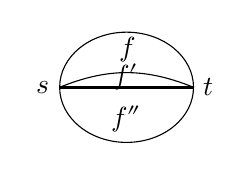
\begin{tikzpicture}[x=1cm,y=1cm,baseline=(current bounding box.center)] \draw (0,0) ellipse (0.85 and 0.70); \draw (-0.85,0) to[bend left=22] (0.85,0); \draw[line width=1.1pt] (-0.85,0)--(0.85,0); \node at (0,0.48) {$f$}; \node at (0,0.13) {$f'$}; \node at (0,-0.40) {$f''$}; \node[left] at (-0.85,0) {$s$}; \node[right] at (0.85,0) {$t$}; \end{tikzpicture}} $f\cap f''=\{s,t\}$}}{\margin{\diagram{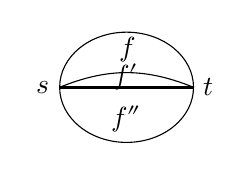
\begin{tikzpicture}[x=1cm,y=1cm,baseline=(current bounding box.center)] \draw (0,0) ellipse (0.85 and 0.70); \draw (-0.85,0) to[bend left=22] (0.85,0); \draw[line width=1.1pt] (-0.85,0)--(0.85,0); \node at (0,0.48) {$f$}; \node at (0,0.13) {$f'$}; \node at (0,-0.40) {$f''$}; \node[left] at (-0.85,0) {$s$}; \node[right] at (0.85,0) {$t$}; \end{tikzpicture}} $f\cap f''=\{s,t\}$}}{marginal note placed}{ps_134-3_010-v0021} \var{\deleted{the}}{}{deletion}{ps_134-3_010-v0022}\var{\inserted{a}}{\hand{a}}{insertion}{ps_134-3_010-v0023} standard example\hand{.} \hand{\unsure{$\ell$}} \var{\over{o}{O}}{\hand{O}}{writing over}{ps_134-3_010-v0024}f lesser import is the misstatement \var{\inserted{(in section 2)}}{\hand{(in section 2)}}{insertion}{ps_134-3_010-v0025} \var{\deleted{on p.2'}}{}{deletion}{ps_134-3_010-v0026},
stating that the associativity relation for the operation \hand{$*_\ell$} should be
\var{\xout{wherexfxf"xisxaxtwo-pointxspacex$\underline{S}_o$xxx}}{}{typewriter deletion}{ps_134-3_010-v0027} replaced by a homotopy arrow
$(\hand{\lambda}*\hand{\mu})*\hand{\nu} \to \hand{\lambda}*(\hand{\mu}*\hand{\nu})$. This is OK for \hand{$\ell$}=1 (primary composition), but
already for \hand{$\ell$}=2 does not make sense as stated, because the sources and
the targets of the two compositions to be compared are not equal, but
only homotopic. Here the statement should be replaced by one making
sense, with a homotopy ``making commutative'' a certain square, and accor\hand{\unsure{-}}%
dingly for cubes etc for higher order co\var{\xout{mp}}{}{typewriter deletion}{ps_134-3_010-v0028}mpositions \hand{$\lambda *_\ell \mu$}, to give rea-%
sonable meaning to associativity. Anyhow, such painstaking explicita-%
tions of particular coherence properties (rather, coherence homotopies)
is kind of ruled out by the sweeping axiomatic description of the
kind of structure species we want for a ``stack'', at least\hand{,} I guess\hand{,} in

%% END SOURCE ps_134-3_010
\ifnum\EditionMode=1
\psapparatusstart
\psentry{ps_134-3_010-v0001}{1}{writing over}{\over{\unsure{18}}{18}}{\hand{18}}{The superposed handwritten reading replaces the underlying reading.}
\psentry{ps_134-3_010-v0002}{2}{insertion}{\inserted{(section 13)}}{\hand{(section 13)}}{The handwritten insertion is incorporated at its indicated position; insertion brackets leave the running text.}
\psentry{ps_134-3_010-v0003}{3}{deletion}{\deleted{\unsure{p.11'}}}{}{The author cancels this material by hand; it leaves the corrected running text.}
\psentry{ps_134-3_010-v0004}{4}{typewriter deletion}{\xout{thatxix}}{}{The typewriter strikes out this material; it leaves the corrected running text.}
\psentry{ps_134-3_010-v0005}{5}{typed insertion}{\inserted[typed]{(contractible)}}{(contractible)}{The typed insertion is incorporated at its indicated position; insertion brackets leave the running text.}
\psentry{ps_134-3_010-v0006}{6}{typewriter deletion}{\xout{x}}{}{The typewriter strikes out this material; it leaves the corrected running text.}
\psentry{ps_134-3_010-v0007}{7}{writing over}{\over{\unsure{at}}{ich}}{\hand{ich}}{The superposed handwritten reading replaces the underlying reading.}
\psentry{ps_134-3_010-v0008}{8}{typewriter deletion}{\xout{n}}{}{The typewriter strikes out this material; it leaves the corrected running text.}
\psentry{ps_134-3_010-v0009}{9}{typed insertion}{\inserted[typed]{strict}}{strict}{The typed insertion is incorporated at its indicated position; insertion brackets leave the running text.}
\psentry{ps_134-3_010-v0010}{10}{typewriter deletion}{\xout{x}}{}{The typewriter strikes out this material; it leaves the corrected running text.}
\psentry{ps_134-3_010-v0011}{11}{insertion}{\inserted{too}}{\hand{too}}{The handwritten insertion is incorporated at its indicated position; insertion brackets leave the running text.}
\psentry{ps_134-3_010-v0012}{12}{insertion}{\inserted{there}}{\hand{there}}{The handwritten insertion is incorporated at its indicated position; insertion brackets leave the running text.}
\psentry{ps_134-3_010-v0013}{13}{deletion}{\deleted{on p.11'}}{}{The author cancels this material by hand; it leaves the corrected running text.}
\psentry{ps_134-3_010-v0014}{14}{typewriter deletion}{\xout{xxxx}}{}{The typewriter strikes out this material; it leaves the corrected running text.}
\psentry{ps_134-3_010-v0015}{15}{typed insertion}{\inserted[typed]{total}}{total}{The typed insertion is incorporated at its indicated position; insertion brackets leave the running text.}
\psentry{ps_134-3_010-v0016}{16}{typewriter deletion}{\xout{xxxxxx}}{}{The typewriter strikes out this material; it leaves the corrected running text.}
\psentry{ps_134-3_010-v0017}{17}{insertion}{\inserted{(section 7)}}{\hand{(section 7)}}{The handwritten insertion is incorporated at its indicated position; insertion brackets leave the running text.}
\psentry{ps_134-3_010-v0018}{18}{deletion}{\deleted{p.7'}}{}{The author cancels this material by hand; it leaves the corrected running text.}
\psentry{ps_134-3_010-v0019}{19}{writing over}{\over{d}{y}}{\hand{y}}{The superposed handwritten reading replaces the underlying reading.}
\psentry{ps_134-3_010-v0020}{20}{typed insertion}{\inserted[typed]{maximal}}{maximal}{The typed insertion is incorporated at its indicated position; insertion brackets leave the running text.}
\psentry{ps_134-3_010-v0021}{21}{marginal note placed}{\margin{\diagram{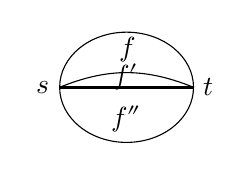
\begin{tikzpicture}[x=1cm,y=1cm,baseline=(current bounding box.center)] \draw (0,0) ellipse (0.85 and 0.70); \draw (-0.85,0) to[bend left=22] (0.85,0); \draw[line width=1.1pt] (-0.85,0)--(0.85,0); \node at (0,0.48) {$f$}; \node at (0,0.13) {$f'$}; \node at (0,-0.40) {$f''$}; \node[left] at (-0.85,0) {$s$}; \node[right] at (0.85,0) {$t$}; \end{tikzpicture}} $f\cap f''=\{s,t\}$}}{\margin{\diagram{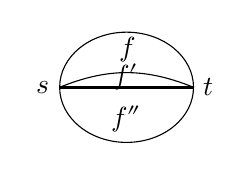
\begin{tikzpicture}[x=1cm,y=1cm,baseline=(current bounding box.center)] \draw (0,0) ellipse (0.85 and 0.70); \draw (-0.85,0) to[bend left=22] (0.85,0); \draw[line width=1.1pt] (-0.85,0)--(0.85,0); \node at (0,0.48) {$f$}; \node at (0,0.13) {$f'$}; \node at (0,-0.40) {$f''$}; \node[left] at (-0.85,0) {$s$}; \node[right] at (0.85,0) {$t$}; \end{tikzpicture}} $f\cap f''=\{s,t\}$}}{The marginal material is set at its source-line call; any internal cancellations and replacements are applied in the corrected form.}
\psentry{ps_134-3_010-v0022}{22}{deletion}{\deleted{the}}{}{The author cancels this material by hand; it leaves the corrected running text.}
\psentry{ps_134-3_010-v0023}{23}{insertion}{\inserted{a}}{\hand{a}}{The handwritten insertion is incorporated at its indicated position; insertion brackets leave the running text.}
\psentry{ps_134-3_010-v0024}{24}{writing over}{\over{o}{O}}{\hand{O}}{The superposed handwritten reading replaces the underlying reading.}
\psentry{ps_134-3_010-v0025}{25}{insertion}{\inserted{(in section 2)}}{\hand{(in section 2)}}{The handwritten insertion is incorporated at its indicated position; insertion brackets leave the running text.}
\psentry{ps_134-3_010-v0026}{26}{deletion}{\deleted{on p.2'}}{}{The author cancels this material by hand; it leaves the corrected running text.}
\psentry{ps_134-3_010-v0027}{27}{typewriter deletion}{\xout{wherexfxf"xisxaxtwo-pointxspacex$\underline{S}_o$xxx}}{}{The typewriter strikes out this material; it leaves the corrected running text.}
\psentry{ps_134-3_010-v0028}{28}{typewriter deletion}{\xout{mp}}{}{The typewriter strikes out this material; it leaves the corrected running text.}
\psapparatusend
\fi
\pssource{ps_134-3_011}{134-3/11}{https://grothendieck.umontpellier.fr/web/viewer.html?file=../134-3.pdf\#page=12}
\psnumber{ps_134-3_011-v0001}{1}
\psnumber{ps_134-3_011-v0002}{2}
\psnumber{ps_134-3_011-v0003}{3}
\psnumber{ps_134-3_011-v0004}{4}
\psnumber{ps_134-3_011-v0005}{5}
\psnumber{ps_134-3_011-v0006}{6}
\psnumber{ps_134-3_011-v0007}{7}
\psnumber{ps_134-3_011-v0008}{8}
\psnumber{ps_134-3_011-v0009}{9}
\psnumber{ps_134-3_011-v0010}{10}
\psnumber{ps_134-3_011-v0011}{11}
\psnumber{ps_134-3_011-v0012}{12}
\psnumber{ps_134-3_011-v0013}{13}
\psnumber{ps_134-3_011-v0014}{14}
\psnumber{ps_134-3_011-v0015}{15}
\psnumber{ps_134-3_011-v0016}{16}
\psnumber{ps_134-3_011-v0017}{17}
\psnumber{ps_134-3_011-v0018}{18}
\psnumber{ps_134-3_011-v0019}{19}
%% BEGIN SOURCE ps_134-3_011
% Pursuing Stacks (cotes 134-2 to 134-8): archive cote 134-3, site page 11 (PDF page 12), typescript page 11.
% typescript. Draft compared: ps2.tex:470-531.
% AI-transcribed by Claude Opus 5.5 (claude-opus-5-5, adaptive thinking, effort high), Message Batches API, batch ps1 (msgbatch_01Rv5hCaNTtUt4JHx1yqoHPL), 2026-11-12; image review recorded in records/CHECK_DECISIONS_134_3_4.tsv.
\scanpage{134-3/11}
\mspage{11}
a large part of the development of the theory of Gr-stacks.  A systematic
study of particular sets of homotopies is closely connected \var{\inserted{of course}}{\hand{of course}}{insertion}{ps_134-3_011-v0001} to an inves-%
\hand{(}tigation into irredundancy conditions which can be figured out for a
\var{\inserted{general}}{\hand{general}}{insertion}{ps_134-3_011-v0002} coherator $\underline{C}$ .  This is indeed an interesting topic,  but I decided not
to get involved in this,  unless I am really forced to!

The basic notion which has been peeling out in the reflection (L)
is of course the notion of a coherator.  Concerning terminology,  it oc-%
cured to me that the dual category $\underline{B}_\infty$ to $\underline{C}_\infty$ is more suggestive in some
cases,  for instance because of the topological interpretation attached
to its objects,  and (more technically)  because of formal analogy of
the role of this category,  for developping homotopical algebra,  with
\var{\margin{(11)}}{\margin{(11)}}{marginal note placed}{ps_134-3_011-v0003} the category of the standar\var{\over{\unsure{t}}{d}}{\hand{d}}{writing over}{ps_134-3_011-v0004} (ordered) simplices\hand{(\textsuperscript{11})}.Both mutually dual
objects $\underline{B}_\infty$ , $\underline{C}_\infty$ seem to me to merit a name,  I suggest to call them
respectively \uline{left} and \uline{right} \uline{coherat ors},  or simply \uline{coherators} of course
when for a while it is understood on which side of the mirror we \var{\over{are}{are}}{\hand{are}}{writing over}{ps_134-3_011-v0005}
playing the game.

O\var{\over{n}{n}}{\hand{n}}{writing over}{ps_134-3_011-v0006}e last comment still before taking off for a heuristic voyage
\var{\over{a}{o}}{\hand{o}}{writing over}{ps_134-3_011-v0007}f discovery of stacks\hand{!} I just had a glance at Benabou\hand{'}s expos\hand{\'e} in 1967
of \var{\over{W}{w}}{\hand{w}}{writing over}{ps_134-3_011-v0008}hat he calls ``bicategories''  (Springer Lecture N\var{\over{o}{o}}{\hand{o}}{writing over}{ps_134-3_011-v0009}tes n\textsuperscript{o} 47 ,  p. 1
- 77).  These are non else,  it appears\hand{,} \var{\deleted{\unsure{than}}}{}{deletion}{ps_134-3_011-v0010} than \var{\deleted{(}}{}{deletion}{ps_134-3_011-v0011}\uline{non associative}
2-categories,  namely 2-stacks  in the terminology I am proposing
(but not 2-Gr-stacks  -  namely at is a particular case of a general
notion of oo-stack which  has still to be developped).  The most interes-%
\hand{-}ting feature of this exposé,  it seems to me,  is the systematic refe-%
rence to topological intuition as \var{\inserted[typed]{a}}{a}{typed insertion}{ps_134-3_011-v0012} support for a comprehension of an
algebraic formalism,  notably \var{\inserted[typed]{of}}{of}{typed insertion}{ps_134-3_011-v0013} the structure of various diagrams. His
terminology,  referring to elements of $F_o,F_1,F_2$ respectively as 0-cells,
1-cells and 2-cells,  is quite suggestive of an idea of \var{\deleted{geometric}}{}{deletion}{ps_134-3_011-v0014} \var{\inserted[typed]{topological}}{topological}{typed insertion}{ps_134-3_011-v0015} reali-%
zation of a 2-stack  -  it is not clear from this exposé whether Benabou
has worked out this idea,  nor whether he has made a connection with
Quillen's ideas on axiomatics of homotopy theory,  which appeared the
same year in the same series\hand{(\textsuperscript{14})}. In any case,  in the last section of his
expos\hand{\'e},  he deals with his bicategories formally as with topological
spaces,  much in the same spirit as \hand{(}\var{\inserted{the one}}{\hand{the one}}{insertion}{ps_134-3_011-v0016} I was contemplating since \var{\xout{1975xxxxx}}{}{typewriter deletion}{ps_134-3_011-v0017}
around 1975,  and which is now motivating the present notes.  While
there is no mention of Benabou\hand{'}s ideas in my letters\unsure{\var{\deleted{t}}{}{deletion}{ps_134-3_011-v0018}} to Larry Breen,
it is quite possible that on the unconscious level,  the little I had
heard of his approach on one or two casual occasions,  had entered into
reaction with my own intuitions\hand{,} coming \var{\inserted[typed]{mainly}}{mainly}{typed insertion}{ps_134-3_011-v0019} from geometry and \unsure{hohomological|cohomological}
algebra,  and finally resulted in the program outlined in those letters.

%% END SOURCE ps_134-3_011
\ifnum\EditionMode=1
\psapparatusstart
\psentry{ps_134-3_011-v0001}{1}{insertion}{\inserted{of course}}{\hand{of course}}{The handwritten insertion is incorporated at its indicated position; insertion brackets leave the running text.}
\psentry{ps_134-3_011-v0002}{2}{insertion}{\inserted{general}}{\hand{general}}{The handwritten insertion is incorporated at its indicated position; insertion brackets leave the running text.}
\psentry{ps_134-3_011-v0003}{3}{marginal note placed}{\margin{(11)}}{\margin{(11)}}{The marginal material is set at its source-line call; any internal cancellations and replacements are applied in the corrected form.}
\psentry{ps_134-3_011-v0004}{4}{writing over}{\over{\unsure{t}}{d}}{\hand{d}}{The superposed handwritten reading replaces the underlying reading.}
\psentry{ps_134-3_011-v0005}{5}{writing over}{\over{are}{are}}{\hand{are}}{The superposed handwritten reading replaces the underlying reading.}
\psentry{ps_134-3_011-v0006}{6}{writing over}{\over{n}{n}}{\hand{n}}{The superposed handwritten reading replaces the underlying reading.}
\psentry{ps_134-3_011-v0007}{7}{writing over}{\over{a}{o}}{\hand{o}}{The superposed handwritten reading replaces the underlying reading.}
\psentry{ps_134-3_011-v0008}{8}{writing over}{\over{W}{w}}{\hand{w}}{The superposed handwritten reading replaces the underlying reading.}
\psentry{ps_134-3_011-v0009}{9}{writing over}{\over{o}{o}}{\hand{o}}{The superposed handwritten reading replaces the underlying reading.}
\psentry{ps_134-3_011-v0010}{10}{deletion}{\deleted{\unsure{than}}}{}{The author cancels this material by hand; it leaves the corrected running text.}
\psentry{ps_134-3_011-v0011}{11}{deletion}{\deleted{(}}{}{The author cancels this material by hand; it leaves the corrected running text.}
\psentry{ps_134-3_011-v0012}{12}{typed insertion}{\inserted[typed]{a}}{a}{The typed insertion is incorporated at its indicated position; insertion brackets leave the running text.}
\psentry{ps_134-3_011-v0013}{13}{typed insertion}{\inserted[typed]{of}}{of}{The typed insertion is incorporated at its indicated position; insertion brackets leave the running text.}
\psentry{ps_134-3_011-v0014}{14}{deletion}{\deleted{geometric}}{}{The author cancels this material by hand; it leaves the corrected running text.}
\psentry{ps_134-3_011-v0015}{15}{typed insertion}{\inserted[typed]{topological}}{topological}{The typed insertion is incorporated at its indicated position; insertion brackets leave the running text.}
\psentry{ps_134-3_011-v0016}{16}{insertion}{\inserted{the one}}{\hand{the one}}{The handwritten insertion is incorporated at its indicated position; insertion brackets leave the running text.}
\psentry{ps_134-3_011-v0017}{17}{typewriter deletion}{\xout{1975xxxxx}}{}{The typewriter strikes out this material; it leaves the corrected running text.}
\psentry{ps_134-3_011-v0018}{18}{deletion}{\deleted{t}}{}{The author cancels this material by hand; it leaves the corrected running text.}
\psentry{ps_134-3_011-v0019}{19}{typed insertion}{\inserted[typed]{mainly}}{mainly}{The typed insertion is incorporated at its indicated position; insertion brackets leave the running text.}
\psapparatusend
\fi
\pssource{ps_134-3_012}{134-3/12}{https://grothendieck.umontpellier.fr/web/viewer.html?file=../134-3.pdf\#page=13}
\psnumber{ps_134-3_012-v0001}{1}
\psnumber{ps_134-3_012-v0002}{2}
\psnumber{ps_134-3_012-v0003}{3}
\psnumber{ps_134-3_012-v0004}{4}
\psnumber{ps_134-3_012-v0005}{5}
\psnumber{ps_134-3_012-v0006}{6}
\psnumber{ps_134-3_012-v0007}{7}
\psnumber{ps_134-3_012-v0008}{8}
\psnumber{ps_134-3_012-v0009}{9}
\psnumber{ps_134-3_012-v0010}{10}
\psnumber{ps_134-3_012-v0011}{11}
\psnumber{ps_134-3_012-v0012}{12}
\psnumber{ps_134-3_012-v0013}{13}
\psnumber{ps_134-3_012-v0014}{14}
\psnumber{ps_134-3_012-v0015}{15}
\psnumber{ps_134-3_012-v0016}{16}
\psnumber{ps_134-3_012-v0017}{17}
\psnumber{ps_134-3_012-v0018}{18}
\psnumber{ps_134-3_012-v0019}{19}
%% BEGIN SOURCE ps_134-3_012
% Pursuing Stacks (cotes 134-2 to 134-8): archive cote 134-3, site page 12 (PDF page 13), typescript page 12.
% typescript. Draft compared: ps2.tex:516-584.
% AI-transcribed by Claude Opus 5.5 (claude-opus-5-5, adaptive thinking, effort high), Message Batches API, batch ps1 (msgbatch_01Rv5hCaNTtUt4JHx1yqoHPL), 2026-11-12; image review recorded in records/CHECK_DECISIONS_134_3_4.tsv.
\scanpage{134-3/12}
\mspage{12}

\hand{19.} I would like now to write down a provisional itinerary of the \unsure{voyage}
ahead - namely to make a list of those main features of a theory of
\var{\margin{$\times$}}{\margin{$\times$}}{marginal note placed}{ps_134-3_012-v0001} stacks which are in my mind these days. I will write them down in the
order in which they occur to me - which will be no obligation upon me
to follow this order, when coming back on those features separately to
elaborate somewhat on them\var{\over{,}{.}}{\hand{.}}{writing over}{ps_134-3_012-v0002} \var{\inserted{This I expect to do,}}{\hand{This I expect to do,}}{insertion}{ps_134-3_012-v0003} mainly as a way to check wether the main
notions and intuitions introduced are sound indeed, and otherwise, to
see how to correct them.

1\textsuperscript{o}) Definition of the categories $\underline{B}_o$ and its dual $\underline{C}_o$ , and formal defi-%
nition of left and right coherators. This definition \var{\over{\unsure{will}}{will}}{\hand{will}}{writing over}{ps_134-3_012-v0004} still be a
provisional one, and will presumably have to be adjusted somewhat to
\var{\over{allo}{allo}}{\hand{allo}}{writing over}{ps_134-3_012-v0005}w for the various structures we are looking for in the corresponding
category of Gr-stacks.

2\textsuperscript{o}) Relation between the category of Gr-stacks and the category of
topological spaces, via two adjoint functors, the ``topological realiza-%
tion functor'' $F_{\ast} \hand{\mapsto} \hand{|}F_{\ast}\hand{|}$ , and the ``singular stack functor''
$X \hand{\mapsto} \underline{F}_{\ast}(X)$ . The situation should be formally analogous to the corres-%
ponding situation for semi-simplicial sets versus topological spaces,
the role of the category $\underline{S}_{\ast}$ of standar\var{\over{t}{d}}{\hand{d}}{writing over}{ps_134-3_012-v0006} ordered simplices being taken
by the left coherator $\underline{B}$ we are working with. The main technical diffe-%
rence here is that the category of Gr-stacks is not just the category of
presheaves on $\underline{B}$, but the full subcategory defined by the requirement
that the presheaves considered should transform ``standar\var{\over{t}{d}}{\hand{d}}{writing over}{ps_134-3_012-v0007}'' amalgamated
sums into fibered products. As a matter of fact, the topological rea-%
lization functor $F_{\ast} \hand{\mapsto} \hand{|}F_{\ast}\hand{|}$ could be defined in standar\var{\over{t}{d}}{\hand{d}}{writing over}{ps_134-3_012-v0008} way on the
whole of $\hand{\widehat{\phantom{B}}}\underline{B}$ , in terms of any functor \var{\xout{B}}{}{typewriter deletion}{ps_134-3_012-v0009}
\hand{(*)} \[ \underline{B} \hand{\longrightarrow} \text{(Spaces)} \]
(by the requirement that the extension of this functor to $\hand{\widehat{\phantom{B}}}B$ commutes
with arbitrary direct limits). A second difference with the \var{\inserted{similar,}}{\hand{similar,}}{insertion}{ps_134-3_012-v0010} simplicial
\var{\deleted{similar}}{}{deletion}{ps_134-3_012-v0011} situation \var{\xout{is that}}{}{typewriter deletion}{ps_134-3_012-v0012} lies in the fact that the only really compel-%
ling choice for the functor (*) is it's restriction to $\underline{B}_o$ , in terms
of the cells $\underline{D}_n$ and the standart \hand{``}half-hemisphere \var{\xout{morphisms}}{}{typewriter deletion}{ps_134-3_012-v0013} maps\hand{''} between
these (L, \var{\deleted{\illegible{1}}}{}{deletion}{ps_134-3_012-v0014}\var{\inserted{section 6}}{\hand{section 6}}{insertion}{ps_134-3_012-v0015}). The extension of this functor to $\underline{B}$ is always possi\hand{\unsure{b}}%
le, due to the \var{\inserted[typed]{inductive}}{inductive}{typed insertion}{ps_134-3_012-v0016} construction of $\underline{B}$ and to the interpretation of elements
\var{\margin{\diagram{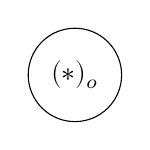
\begin{tikzpicture}[baseline=(n.base)]\node[draw,circle,inner sep=5pt] (n) {$({*})_o$};\end{tikzpicture}}}}{\margin{\diagram{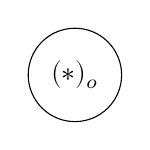
\begin{tikzpicture}[baseline=(n.base)]\node[draw,circle,inner sep=5pt] (n) {$({*})_o$};\end{tikzpicture}}}}{marginal note placed}{ps_134-3_012-v0017} of $\underline{B}_o$ as \uline{contractible} spaces, via the functor (*)\hand{$_o$}; but it depends on
a bunch of arbitrary choices. To give precise meaning to the intuition
that these choices do\var{\over{nt}{'nt}}{\hand{'nt}}{writing over}{ps_134-3_012-v0018} really make a difference, and that the choic\unsure{e}
\var{\inserted[typed]{of}}{of}{typed insertion}{ps_134-3_012-v0019} coherator we are starting with does'nt make much of a difference either\hand{,}
will need some elaboration on the notion of \uline{equivalences between}

%% END SOURCE ps_134-3_012
\ifnum\EditionMode=1
\psapparatusstart
\psentry{ps_134-3_012-v0001}{1}{marginal note placed}{\margin{$\times$}}{\margin{$\times$}}{The marginal material is set at its source-line call; any internal cancellations and replacements are applied in the corrected form.}
\psentry{ps_134-3_012-v0002}{2}{writing over}{\over{,}{.}}{\hand{.}}{The superposed handwritten reading replaces the underlying reading.}
\psentry{ps_134-3_012-v0003}{3}{insertion}{\inserted{This I expect to do,}}{\hand{This I expect to do,}}{The handwritten insertion is incorporated at its indicated position; insertion brackets leave the running text.}
\psentry{ps_134-3_012-v0004}{4}{writing over}{\over{\unsure{will}}{will}}{\hand{will}}{The superposed handwritten reading replaces the underlying reading.}
\psentry{ps_134-3_012-v0005}{5}{writing over}{\over{allo}{allo}}{\hand{allo}}{The superposed handwritten reading replaces the underlying reading.}
\psentry{ps_134-3_012-v0006}{6}{writing over}{\over{t}{d}}{\hand{d}}{The superposed handwritten reading replaces the underlying reading.}
\psentry{ps_134-3_012-v0007}{7}{writing over}{\over{t}{d}}{\hand{d}}{The superposed handwritten reading replaces the underlying reading.}
\psentry{ps_134-3_012-v0008}{8}{writing over}{\over{t}{d}}{\hand{d}}{The superposed handwritten reading replaces the underlying reading.}
\psentry{ps_134-3_012-v0009}{9}{typewriter deletion}{\xout{B}}{}{The typewriter strikes out this material; it leaves the corrected running text.}
\psentry{ps_134-3_012-v0010}{10}{insertion}{\inserted{similar,}}{\hand{similar,}}{The handwritten insertion is incorporated at its indicated position; insertion brackets leave the running text.}
\psentry{ps_134-3_012-v0011}{11}{deletion}{\deleted{similar}}{}{The author cancels this material by hand; it leaves the corrected running text.}
\psentry{ps_134-3_012-v0012}{12}{typewriter deletion}{\xout{is that}}{}{The typewriter strikes out this material; it leaves the corrected running text.}
\psentry{ps_134-3_012-v0013}{13}{typewriter deletion}{\xout{morphisms}}{}{The typewriter strikes out this material; it leaves the corrected running text.}
\psentry{ps_134-3_012-v0014}{14}{deletion}{\deleted{\illegible{1}}}{}{The author cancels this material by hand; it leaves the corrected running text.}
\psentry{ps_134-3_012-v0015}{15}{insertion}{\inserted{section 6}}{\hand{section 6}}{The handwritten insertion is incorporated at its indicated position; insertion brackets leave the running text.}
\psentry{ps_134-3_012-v0016}{16}{typed insertion}{\inserted[typed]{inductive}}{inductive}{The typed insertion is incorporated at its indicated position; insertion brackets leave the running text.}
\psentry{ps_134-3_012-v0017}{17}{marginal note placed}{\margin{\diagram{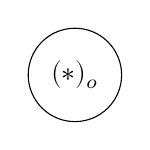
\begin{tikzpicture}[baseline=(n.base)]\node[draw,circle,inner sep=5pt] (n) {$({*})_o$};\end{tikzpicture}}}}{\margin{\diagram{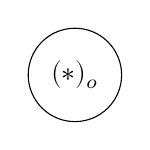
\begin{tikzpicture}[baseline=(n.base)]\node[draw,circle,inner sep=5pt] (n) {$({*})_o$};\end{tikzpicture}}}}{The marginal material is set at its source-line call; any internal cancellations and replacements are applied in the corrected form.}
\psentry{ps_134-3_012-v0018}{18}{writing over}{\over{nt}{'nt}}{\hand{'nt}}{The superposed handwritten reading replaces the underlying reading.}
\psentry{ps_134-3_012-v0019}{19}{typed insertion}{\inserted[typed]{of}}{of}{The typed insertion is incorporated at its indicated position; insertion brackets leave the running text.}
\psapparatusend
\fi
\pssource{ps_134-3_013}{134-3/13}{https://grothendieck.umontpellier.fr/web/viewer.html?file=../134-3.pdf\#page=14}
\psnumber{ps_134-3_013-v0001}{1}
\psnumber{ps_134-3_013-v0002}{2}
\psnumber{ps_134-3_013-v0003}{3}
\psnumber{ps_134-3_013-v0004}{4}
\psnumber{ps_134-3_013-v0005}{5}
\psnumber{ps_134-3_013-v0006}{6}
\psnumber{ps_134-3_013-v0007}{7}
\psnumber{ps_134-3_013-v0008}{8}
\psnumber{ps_134-3_013-v0009}{9}
\psnumber{ps_134-3_013-v0010}{10}
\psnumber{ps_134-3_013-v0011}{11}
\psnumber{ps_134-3_013-v0012}{12}
\psnumber{ps_134-3_013-v0013}{13}
\psnumber{ps_134-3_013-v0014}{14}
%% BEGIN SOURCE ps_134-3_013
% Pursuing Stacks (cotes 134-2 to 134-8): archive cote 134-3, site page 13 (PDF page 14), typescript page 13.
% typescript. Draft compared: ps2.tex:569-633.
% AI-transcribed by Claude Opus 5.5 (claude-opus-5-5, adaptive thinking, effort high), Message Batches API, batch ps1 (msgbatch_01Rv5hCaNTtUt4JHx1yqoHPL), 2026-11-12; image review recorded in records/CHECK_DECISIONS_134_3_4.tsv.
\scanpage{134-3/13}
\mspage{13}
Gr-\uline{stacks}, which will have to \var{\xout{tx}}{}{typewriter deletion}{ps_134-3_013-v0001} be developped at a later stage.

The idea just comes to my mind whether the exactness condition
implying standar\var{\over{t}{d}}{\hand{d}}{writing over}{ps_134-3_013-v0002} amalgamated sums, defining the subcategory of stacks
within $\overset{\hand{\wedge}}{\underline{B}}$ , cannot be interpreted in terms of some more or less obvious
topology on $\underline{B}$ turning $\underline{B}$ into a site, as the subcategory of correspon-%
ding \uline{sheaves}. This would mean that the category (Gr-stacks) is in fact
a topos, with the host of eategorical information and topological
intuition that goes with such a situation. In this connection, it is
timely to recall that the related categories (Cat) of ``all'' categories,
and (Groupoids) of ``all'' groupoids, are definitely \uline{not} topoi (if my
recollection is correct - it is\hand{'}nt immediately clear to me why they
are not). This seems to suggest that, granting that (Gr-stacks) is
indeed a topos, that this would be a rather special feature of the
structure species of infinite order we are working with (as \var{\deleted{a}}{}{deletion}{ps_134-3_013-v0003}\var{\inserted[typed]{one}}{one}{typed insertion}{ps_134-3_013-v0004} reward so
to say,among a heap of others, for conceptual sophistication !), in
contrast to the categories (Gr-n-stacks)\var{\inserted[typed]{with finite n}}{with finite n}{typed insertion}{ps_134-3_013-v0005}, which presumably are not topoi
(For a definition of Gr-n-stacks in terms of Gr-stacks namely
Gr-$\infty$-stacks, see below.\hand{)}

A related question is whether the category (Gr-stacks) is a model
category for the usual homotopy category, the pair of adjoint functors
bonsidered before satisfying \var{\inserted{moreover}}{\hand{moreover}}{insertion}{ps_134-3_013-v0006} the conditions of Quillen's comparison
theorem\hand{(\textsuperscript{13})}.The obvious idea that comes to mind here, in order to define
the model structure on (Gr-stacks), is to take as ``weak equivalences''
the maps which are transformed into weak equivalences by the topological
realization functor (which should be readily expressible in \var{\inserted[typed]{algebraic}}{algebraic}{typed insertion}{ps_134-3_013-v0007} terms \var{\xout{as}}{}{typewriter deletion}{ps_134-3_013-v0008} ..\hand{)},
\var{\over{\unsure{as}}{as}}{\hand{as}}{writing over}{ps_134-3_013-v0009} cofibrations the monomorphisms, and defining fibrations by the
Serre-Quillen lifting property with respect to cofibrations which are
weak equivalences (with the expectation that we even get a ``closed mod\hand{el}
category'' in the sense of Quillen). Here it does'nt look too unreasonab
\hand{-}le to expect the same constructions to work in each of the categories
(Gr-n-stacks), n \var{\over{$>$}{$\geqslant$}}{\hand{$\geqslant$}}{writing over}{ps_134-3_013-v0010}1, as well as in the categories (n-stacks) without
Gr , which are still to be defined though.

Coming back upon the question of a suitable topology on $\underline{B}$, the
idea that comes to mind immediately of course is to define\var{\deleted{s}}{}{deletion}{ps_134-3_013-v0011} covering
families of an object K of $\underline{B}$ i.e. of $\underline{B}_o$ , in terms of the components
which occur in the description of K as an \var{\inserted[typed]{iterated}}{iterated}{typed insertion}{ps_134-3_013-v0012} amalgamated sum of\var{\deleted{\unsure{s}}}{}{deletion}{ps_134-3_013-v0013} cells $D_n$.
A quick glance (too quick a glance ?) seems to show this is indeed a
topology, and that the sheaves for this topology are what we expect.
\var{\deleted{This would imply that the \deleted{inclusion} \inserted{composite} functor}}{}{deletion}{ps_134-3_013-v0014}

%% END SOURCE ps_134-3_013
\ifnum\EditionMode=1
\psapparatusstart
\psentry{ps_134-3_013-v0001}{1}{typewriter deletion}{\xout{tx}}{}{The typewriter strikes out this material; it leaves the corrected running text.}
\psentry{ps_134-3_013-v0002}{2}{writing over}{\over{t}{d}}{\hand{d}}{The superposed handwritten reading replaces the underlying reading.}
\psentry{ps_134-3_013-v0003}{3}{deletion}{\deleted{a}}{}{The author cancels this material by hand; it leaves the corrected running text.}
\psentry{ps_134-3_013-v0004}{4}{typed insertion}{\inserted[typed]{one}}{one}{The typed insertion is incorporated at its indicated position; insertion brackets leave the running text.}
\psentry{ps_134-3_013-v0005}{5}{typed insertion}{\inserted[typed]{with finite n}}{with finite n}{The typed insertion is incorporated at its indicated position; insertion brackets leave the running text.}
\psentry{ps_134-3_013-v0006}{6}{insertion}{\inserted{moreover}}{\hand{moreover}}{The handwritten insertion is incorporated at its indicated position; insertion brackets leave the running text.}
\psentry{ps_134-3_013-v0007}{7}{typed insertion}{\inserted[typed]{algebraic}}{algebraic}{The typed insertion is incorporated at its indicated position; insertion brackets leave the running text.}
\psentry{ps_134-3_013-v0008}{8}{typewriter deletion}{\xout{as}}{}{The typewriter strikes out this material; it leaves the corrected running text.}
\psentry{ps_134-3_013-v0009}{9}{writing over}{\over{\unsure{as}}{as}}{\hand{as}}{The superposed handwritten reading replaces the underlying reading.}
\psentry{ps_134-3_013-v0010}{10}{writing over}{\over{$>$}{$\geqslant$}}{\hand{$\geqslant$}}{The superposed handwritten reading replaces the underlying reading.}
\psentry{ps_134-3_013-v0011}{11}{deletion}{\deleted{s}}{}{The author cancels this material by hand; it leaves the corrected running text.}
\psentry{ps_134-3_013-v0012}{12}{typed insertion}{\inserted[typed]{iterated}}{iterated}{The typed insertion is incorporated at its indicated position; insertion brackets leave the running text.}
\psentry{ps_134-3_013-v0013}{13}{deletion}{\deleted{\unsure{s}}}{}{The author cancels this material by hand; it leaves the corrected running text.}
\psentry{ps_134-3_013-v0014}{14}{deletion}{\deleted{This would imply that the \deleted{inclusion} \inserted{composite} functor}}{}{The author cancels this material by hand; it leaves the corrected running text.}
\psapparatusend
\fi
\pssource{ps_134-3_014}{134-3/14}{https://grothendieck.umontpellier.fr/web/viewer.html?file=../134-3.pdf\#page=15}
\psnumber{ps_134-3_014-v0001}{1}
\psnumber{ps_134-3_014-v0002}{2}
\psnumber{ps_134-3_014-v0003}{3}
\psnumber{ps_134-3_014-v0004}{4}
\psnumber{ps_134-3_014-v0005}{5}
\psnumber{ps_134-3_014-v0006}{6}
\psnumber{ps_134-3_014-v0007}{7}
\psnumber{ps_134-3_014-v0008}{8}
\psnumber{ps_134-3_014-v0009}{9}
\psnumber{ps_134-3_014-v0010}{10}
%% BEGIN SOURCE ps_134-3_014
% Pursuing Stacks (cotes 134-2 to 134-8): archive cote 134-3, site page 14 (PDF page 15), typescript page 14.
% typescript. Draft compared: ps2.tex:616-682.
% AI-transcribed by Claude Opus 5.5 (claude-opus-5-5, adaptive thinking, effort high), Message Batches API, batch ps1 (msgbatch_01Rv5hCaNTtUt4JHx1yqoHPL), 2026-11-12; image review recorded in records/CHECK_DECISIONS_134_3_4.tsv.
\scanpage{134-3/14}
\hand{5}.3. \mspage{\hand{14}}

\hand{20.} I had barely st opped writing last tuesday,  when it became clear \var{\xout{th}}{}{typewriter deletion}{ps_134-3_014-v0001}
that the ``quick glance'' had been too quick indeed. \var{\xout{It would}}{}{typewriter deletion}{ps_134-3_014-v0002} As a matter
of fact,  the ``topology'' I was contemplating on $\underline{B}$ in terms of covering
families does not satisfy the conditions for a ``site'' -  that something
was fishy first occured to me through the heuristic consequence,  that
the functors  ``n-th component''
\[ F_{*} \hand{\longmapsto} F_{n} \]
from \var{\xout{\illegible{1}}}{}{typewriter deletion}{ps_134-3_014-v0003} stacks to sets are fiber functors,  or equivalently, that
direct limits in the category of Gr-stacks can be computed componentwise
-  now this is definitely false,  for much the same reasons why it is
false \unsure{already|alfeady} in the category (Cat) of categories.  However,  it occured
to me that \var{\inserted{in}}{\hand{in}}{insertion}{ps_134-3_014-v0004} the latter category (Cat),  although not a topos (for instan-%
ce because, according to Giraud's paper on descent theory of 1965\hand{, (19)}
the implications for epimorphisms
\diagram{
% Hand-drawn arrows are marked blue; typed objects remain plain.
\begin{tikzcd}[row sep=tiny,column sep=large]
 \& \text{effective} \arrow[dr, Rightarrow, color=blue] \& \\
\text{effective universal} \arrow[ur, Rightarrow, color=blue] \arrow[dr, Rightarrow, color=blue] \& \& \text{just epi} \\
 \& \text{universal} \arrow[ur, Rightarrow, color=blue] \&
\end{tikzcd}
}
are strict),  there \uline{is} a very natural topology,  \var{\xout{namely}}{}{typewriter deletion}{ps_134-3_014-v0005} turning it into
a site,  namely the one where a family of morphisms namely functors
\[ A_{i} \hand{\longrightarrow} A \]
is covering if and only if the corresponding family in (Ss sets)
\[ \mathrm{Nerve}(A_{i}) \hand{\longrightarrow} \mathrm{Nerve}(A) \]
is covering,  i.e. iff every \var{\xout{family}}{}{typewriter deletion}{ps_134-3_014-v0006} sequence of composable arrows in A
\[ a_{0} \hand{\to} a_{1} \hand{\to} a_{2} \hand{\to} a_{3} \hand{\to} \quad \dots \hand{\to} a_{n} \]
can be lifted  to one among the $A_{i}$'s.  As a matter of fact,  this condi-%
\var{\margin{\unsure{5.3. This is definitely false, see \S24 below}}}{\margin{\unsure{5.3. This is definitely false, see \S24 below}}}{marginal note placed}{ps_134-3_014-v0007}
tion (where it suffices to take n=2,  visibly)  is equivalent (according
to Giraud) to the condition that the family be \hand{``}universally effectively
epimorphic\hand{''},  i.e. covering with respect to the``canonical topology''of
(Cat)\hand{(15)}.This suggests a third way for associating to a \var{\inserted{[small]}}{\hand{[small]}}{insertion}{ps_134-3_014-v0008} category A a
topology-like structure,  namely the topos of all sheaves over
$(\mathrm{Cat})_{/A}$  ,  the site of all categories over A, \var{\inserted[typed]{endowed}}{endowed}{typed insertion}{ps_134-3_014-v0009} with the topology induced
by the canonical topology of (Cat)  (which is indeed the canonical topo\hand{-}%
logy of  $(\mathrm{Cat})_{/A}$ \hand{)}.  It should be an easy exercice in terms of nerves to
check that the homotopy type (a priori,  a prohomotopy type)  associated
to this site is just \hand{``}the\hand{''}homotopy type of A,  defined either as the
homotopy type of Nerve(A),  or as the (pro)homotopy type of the topos
$\overset{\hand{\wedge}}{A}$ of all presheaves over A.  This of course parallels the similar fami-%
liar fact in the category (Ss sets) of all semisimplicial sets,  namely
that for such a ss set\var{\deleted{\unsure{s}}}{}{deletion}{ps_134-3_014-v0010} K,  the homotopy type of K can be viewed also
as the homotopy type of the induce\hand{d} topos  $(\mathrm{Ss\ sets})_{/K}$ of all ss sets
over K.  The difference in the two cases is that  in the second case

%% END SOURCE ps_134-3_014
\ifnum\EditionMode=1
\psapparatusstart
\psentry{ps_134-3_014-v0001}{1}{typewriter deletion}{\xout{th}}{}{The typewriter strikes out this material; it leaves the corrected running text.}
\psentry{ps_134-3_014-v0002}{2}{typewriter deletion}{\xout{It would}}{}{The typewriter strikes out this material; it leaves the corrected running text.}
\psentry{ps_134-3_014-v0003}{3}{typewriter deletion}{\xout{\illegible{1}}}{}{The typewriter strikes out this material; it leaves the corrected running text.}
\psentry{ps_134-3_014-v0004}{4}{insertion}{\inserted{in}}{\hand{in}}{The handwritten insertion is incorporated at its indicated position; insertion brackets leave the running text.}
\psentry{ps_134-3_014-v0005}{5}{typewriter deletion}{\xout{namely}}{}{The typewriter strikes out this material; it leaves the corrected running text.}
\psentry{ps_134-3_014-v0006}{6}{typewriter deletion}{\xout{family}}{}{The typewriter strikes out this material; it leaves the corrected running text.}
\psentry{ps_134-3_014-v0007}{7}{marginal note placed}{\margin{\unsure{5.3. This is definitely false, see \S24 below}}}{\margin{\unsure{5.3. This is definitely false, see \S24 below}}}{The marginal material is set at its source-line call; any internal cancellations and replacements are applied in the corrected form.}
\psentry{ps_134-3_014-v0008}{8}{insertion}{\inserted{[small]}}{\hand{[small]}}{The handwritten insertion is incorporated at its indicated position; insertion brackets leave the running text.}
\psentry{ps_134-3_014-v0009}{9}{typed insertion}{\inserted[typed]{endowed}}{endowed}{The typed insertion is incorporated at its indicated position; insertion brackets leave the running text.}
\psentry{ps_134-3_014-v0010}{10}{deletion}{\deleted{\unsure{s}}}{}{The author cancels this material by hand; it leaves the corrected running text.}
\psapparatusend
\fi
\pssource{ps_134-3_015}{134-3/15}{https://grothendieck.umontpellier.fr/web/viewer.html?file=../134-3.pdf\#page=16}
\psnumber{ps_134-3_015-v0001}{1}
\psnumber{ps_134-3_015-v0002}{2}
\psnumber{ps_134-3_015-v0003}{3}
\psnumber{ps_134-3_015-v0004}{4}
\psnumber{ps_134-3_015-v0005}{5}
\psnumber{ps_134-3_015-v0006}{6}
\psnumber{ps_134-3_015-v0007}{7}
\psnumber{ps_134-3_015-v0008}{8}
\psnumber{ps_134-3_015-v0009}{9}
\psnumber{ps_134-3_015-v0010}{10}
\psnumber{ps_134-3_015-v0011}{11}
\psnumber{ps_134-3_015-v0012}{12}
\psnumber{ps_134-3_015-v0013}{13}
\psnumber{ps_134-3_015-v0014}{14}
\psnumber{ps_134-3_015-v0015}{15}
\psnumber{ps_134-3_015-v0016}{16}
\psnumber{ps_134-3_015-v0017}{17}
%% BEGIN SOURCE ps_134-3_015
% Pursuing Stacks (cotes 134-2 to 134-8): archive cote 134-3, site page 15 (PDF page 16), typescript page 15.
% typescript. Draft compared: ps2.tex:669-728.
% AI-transcribed by Claude Opus 5.5 (claude-opus-5-5, adaptive thinking, effort high), Message Batches API, batch ps1 (msgbatch_01Rv5hCaNTtUt4JHx1yqoHPL), 2026-11-12; image review recorded in records/CHECK_DECISIONS_134_3_4.tsv.
\scanpage{134-3/15}
\mspage{15}

the category  (Ss sets) (and hence \var{\over{\unsure{the}}{any}}{\hand{any}}{writing over}{ps_134-3_015-v0001} induced categor\var{\over{\unsure{ies}}{y}}{\hand{y}}{writing over}{ps_134-3_015-v0002}) \var{\over{\unsure{are}}{is}}{\hand{is}}{writing over}{ps_134-3_015-v0003} already
a topos,  namely equivalent to the category of sheaves on the same for
the canonical topology,  whereas in the category (Cat)  this is not so.

These reflections suggest that in most if not all categories of
models encountered for describing usual homotopy types,  there is a \var{\margin{\unsure{5.3. this presumption is false actually}}}{\margin{\unsure{5.3. this presumption is false actually}}}{marginal note placed}{ps_134-3_015-v0004}
natural structure of a site on the model category M (\uline{presumably} the one
corresponding to the canonical topology(\var{\over{*}{15}}{\hand{15}}{writing over}{ps_134-3_015-v0005})), with the property that the
homotopy type of any object X in M is \var{\xout{also}}{}{typewriter deletion}{ps_134-3_015-v0006} canonically isomorphic to the
(pro)homotopy type of the induced site $M_{/X}$ ,  or what amount\hand{s} to the same,
of the corresponding topos
\[ (M_{/X})^{\hand{\sim}} \;=\; M^{\hand{\sim}}_{/X} \;. \]
I would expect definitely this to be the case for each of the categories
(Gr-stacks), (n-Gr-stacks) (although this is not really a model category
in the sense of Quillen,\hand{as} it gives rise only to n-truncated homotopy
types ...),  (stacks)  and (n-stacks),  corresponding to an arbitrary \var{\margin{$\lceil$}}{\margin{$\lceil$}}{marginal note placed}{ps_134-3_015-v0007}
choice of a coherator,  defining the notion of a (Gr-stack),  or of a \var{\margin{$[$}}{\margin{$[$}}{marginal note placed}{ps_134-3_015-v0008}
stack  (for the latter and relations between the two,  see below). \var{\margin{$\lfloor$}}{\margin{$\lfloor$}}{marginal note placed}{ps_134-3_015-v0009}

\var{\margin{$|$}}{\margin{$|$}}{marginal note placed}{ps_134-3_015-v0010}\unsure{\var{\over{1}{2}}{\hand{2}}{writing over}{ps_134-3_015-v0011}}1.  I would like to digress a little more,  to emphasize still about
\var{\margin{$\downarrow$}}{\margin{$\downarrow$}}{marginal note placed}{ps_134-3_015-v0012}the vast variety of algebraic structures giving rise to model categories
for the usual homotopy category,  or at any rate suitable for expressing
more or less arbitrary homotopy types.  Apart from stacks,  where every
thing is still heuristics for the time being,  we have noticed so far
three examples of such structures,  namely  ss complexes,  cubical com-%
plexes,  and categories.  There are a  few familiar variants of the two
former,  such as the  ``simplicial complexes'' (in contrast to semi-simpli
cial ones) ,  namely \var{\inserted[typed]{presheaves on}}{presheaves on}{typed insertion}{ps_134-3_015-v0013} \var{\xout{functors from}}{}{typewriter deletion}{ps_134-3_015-v0014} the category of non-empty finite sets\hand{,}
which can be interpreted as ss complexes enriched with symmetry operati-%
ons on each component  -  and there is the corresponding variant in the
cubical case.  It would be rather surprising that these were not just
as good model categories,  as the more habitual ones (\var{\over{*}{16}}{\hand{16}}{writing over}{ps_134-3_015-v0015}) - all the more
as the singular complex (simplicial or cubical) is naturally endowed
with this extra structure,  which one generally chooses to forget. More
interesting variants are the  n-multicomplexes (simplicial or cubical,
with or without symmetries),  defined \hand{by} \var{\xout{presheaves}}{}{typewriter deletion}{ps_134-3_015-v0016} contravariant func-%
tors to sets  in n arguments rather than in just one,  where $n\hand{\geqslant}\hand{1}$. The-%
se complexes are familiar mainly,  it seems,  because of their connecti\hand{\unsure{on|ons}}
with product spaces and the Künneth-Eilenberg-Zilber type relations.
It is generally understood that to such a\var{\xout{n}}{}{typewriter deletion}{ps_134-3_015-v0017} multicomplex is associated

%% END SOURCE ps_134-3_015
\ifnum\EditionMode=1
\psapparatusstart
\psentry{ps_134-3_015-v0001}{1}{writing over}{\over{\unsure{the}}{any}}{\hand{any}}{The superposed handwritten reading replaces the underlying reading.}
\psentry{ps_134-3_015-v0002}{2}{writing over}{\over{\unsure{ies}}{y}}{\hand{y}}{The superposed handwritten reading replaces the underlying reading.}
\psentry{ps_134-3_015-v0003}{3}{writing over}{\over{\unsure{are}}{is}}{\hand{is}}{The superposed handwritten reading replaces the underlying reading.}
\psentry{ps_134-3_015-v0004}{4}{marginal note placed}{\margin{\unsure{5.3. this presumption is false actually}}}{\margin{\unsure{5.3. this presumption is false actually}}}{The marginal material is set at its source-line call; any internal cancellations and replacements are applied in the corrected form.}
\psentry{ps_134-3_015-v0005}{5}{writing over}{\over{*}{15}}{\hand{15}}{The superposed handwritten reading replaces the underlying reading.}
\psentry{ps_134-3_015-v0006}{6}{typewriter deletion}{\xout{also}}{}{The typewriter strikes out this material; it leaves the corrected running text.}
\psentry{ps_134-3_015-v0007}{7}{marginal note placed}{\margin{$\lceil$}}{\margin{$\lceil$}}{The marginal material is set at its source-line call; any internal cancellations and replacements are applied in the corrected form.}
\psentry{ps_134-3_015-v0008}{8}{marginal note placed}{\margin{$[$}}{\margin{$[$}}{The marginal material is set at its source-line call; any internal cancellations and replacements are applied in the corrected form.}
\psentry{ps_134-3_015-v0009}{9}{marginal note placed}{\margin{$\lfloor$}}{\margin{$\lfloor$}}{The marginal material is set at its source-line call; any internal cancellations and replacements are applied in the corrected form.}
\psentry{ps_134-3_015-v0010}{10}{marginal note placed}{\margin{$|$}}{\margin{$|$}}{The marginal material is set at its source-line call; any internal cancellations and replacements are applied in the corrected form.}
\psentry{ps_134-3_015-v0011}{11}{writing over}{\over{1}{2}}{\hand{2}}{The superposed handwritten reading replaces the underlying reading.}
\psentry{ps_134-3_015-v0012}{12}{marginal note placed}{\margin{$\downarrow$}}{\margin{$\downarrow$}}{The marginal material is set at its source-line call; any internal cancellations and replacements are applied in the corrected form.}
\psentry{ps_134-3_015-v0013}{13}{typed insertion}{\inserted[typed]{presheaves on}}{presheaves on}{The typed insertion is incorporated at its indicated position; insertion brackets leave the running text.}
\psentry{ps_134-3_015-v0014}{14}{typewriter deletion}{\xout{functors from}}{}{The typewriter strikes out this material; it leaves the corrected running text.}
\psentry{ps_134-3_015-v0015}{15}{writing over}{\over{*}{16}}{\hand{16}}{The superposed handwritten reading replaces the underlying reading.}
\psentry{ps_134-3_015-v0016}{16}{typewriter deletion}{\xout{presheaves}}{}{The typewriter strikes out this material; it leaves the corrected running text.}
\psentry{ps_134-3_015-v0017}{17}{typewriter deletion}{\xout{n}}{}{The typewriter strikes out this material; it leaves the corrected running text.}
\psapparatusend
\fi
\pssource{ps_134-3_016}{134-3/16}{https://grothendieck.umontpellier.fr/web/viewer.html?file=../134-3.pdf\#page=17}
\psnumber{ps_134-3_016-v0001}{1}
\psnumber{ps_134-3_016-v0002}{2}
\psnumber{ps_134-3_016-v0003}{3}
\psnumber{ps_134-3_016-v0004}{4}
\psnumber{ps_134-3_016-v0005}{5}
\psnumber{ps_134-3_016-v0006}{6}
\psnumber{ps_134-3_016-v0007}{7}
\psnumber{ps_134-3_016-v0008}{8}
\psnumber{ps_134-3_016-v0009}{9}
\psnumber{ps_134-3_016-v0010}{10}
\psnumber{ps_134-3_016-v0011}{11}
\psnumber{ps_134-3_016-v0012}{12}
\psnumber{ps_134-3_016-v0013}{13}
\psnumber{ps_134-3_016-v0014}{14}
\psnumber{ps_134-3_016-v0015}{15}
\psnumber{ps_134-3_016-v0016}{16}
\psnumber{ps_134-3_016-v0017}{17}
\psnumber{ps_134-3_016-v0018}{18}
\psnumber{ps_134-3_016-v0019}{19}
\psnumber{ps_134-3_016-v0020}{20}
\psnumber{ps_134-3_016-v0021}{21}
\psnumber{ps_134-3_016-v0022}{22}
\psnumber{ps_134-3_016-v0023}{23}
\psnumber{ps_134-3_016-v0024}{24}
\psnumber{ps_134-3_016-v0025}{25}
\psnumber{ps_134-3_016-v0026}{26}
%% BEGIN SOURCE ps_134-3_016
% Pursuing Stacks (cotes 134-2 to 134-8): archive cote 134-3, site page 16 (PDF page 17), typescript page 16.
% typescript. Draft compared: ps2.tex:716-774.
% AI-transcribed by Claude Opus 5.5 (claude-opus-5-5, adaptive thinking, effort high), Message Batches API, batch ps1 (msgbatch_01Rv5hCaNTtUt4JHx1yqoHPL), 2026-11-12; image review recorded in records/CHECK_DECISIONS_134_3_4.tsv.
\scanpage{134-3/16}
\mspage{16}
the corresponding "diagonal" complex,  which is just a usual complex and
adequately describes the "homotopy type" of the multicomplex. So why
bother with relatively messy kind of models,  when just usual complexes
suffice !  Here however the point is not to get the handiest possible
model categories (whatever our cr\var{\over{e}{i}}{\hand{i}}{writing over}{ps_134-3_016-v0001}teria of "handyness"),  but rather to
get an idea of the variety of algebraic structures suitable for defining
homotopy types,  and perhaps to come to a clue of what is common to all
these.  Moreover,  I feel the relation between ordinary comple\var{\over{c}{x}}{\hand{x}}{writing over}{ps_134-3_016-v0002}es,
and n-multicomplexes,  is of much the same nature as the relation bet-%
ween just ordinary categories,  perfectly sufficient for describing homo
-topy types,  and  n-categories  or n-stacks.  This reminds of course of
Quillen's idea of defining n-categories in terms of n-semisimplicial
complexes,  in much the same way as categories can be defined (via the
Nerve functor)  in terms of usual ss complexes.  I hit again upon multi-%
simplices (without symmetry),  when trying to reduce to a \uline{minimum} the
\var{\over{category}{category}}{\hand{category}}{writing over}{ps_134-3_016-v0003} $\underline{B}_o$ of \var{\xout{\unsure{socalled}}}{}{typewriter deletion}{ps_134-3_016-v0004} what should be called "standar\var{\over{t}{d}}{\hand{d}}{writing over}{ps_134-3_016-v0005}"amalgamated
sums of the cells $D_n$ ,  where my tendency initially (L, \var{\deleted{\unsure{p.7}}}{}{deletion}{ps_134-3_016-v0006}\var{\inserted{section 8}}{\hand{section 8}}{insertion}{ps_134-3_016-v0007}) had rather
been to be as generous as possible,  in order to be as stringent as ima-%
ginable  for the completion condition (A)  of (L, \var{\deleted{\unsure{p.8}}}{}{deletion}{ps_134-3_016-v0008}\var{\inserted{section 9}}{\hand{section 9}}{insertion}{ps_134-3_016-v0009}).  Now it turns
out that the coherence relations which seem to have been written down so
far (and \var{\inserted[typed]{the like of}}{the like of}{typed insertion}{ps_134-3_016-v0010} which presumably will suffice to imply full completeness of
coherence relations,  in the sense of (A))  make use only of very restri-%
ted types of such amalgamated sums,  expressible precisely in terms of
multisimplices.  (This I ckecked \var{\inserted[typed]{for instance}}{for instance}{typed insertion}{ps_134-3_016-v0011} on the full list of data and axioms
for Bénabou's "bicategories" namely  2-stacks,  in \hand{his} 1967 Midwest Cate-%
gory Seminar \var{\inserted{exposé}}{\hand{exposé}}{insertion}{ps_134-3_016-v0012} (already referred to.)  I'll have to come back upon this
point with some care,  which gives also a pretty natural way for getting
Quillen's functor from  n-stacks to n-ss complexes.
\var{\margin{\diagram{\begin{tikzpicture}[x=1cm,y=1cm]\draw[->] (0.35,0)--(0,0)--(0,1.1);\end{tikzpicture}}}}{\margin{\diagram{\begin{tikzpicture}[x=1cm,y=1cm]\draw[->] (0.35,0)--(0,0)--(0,1.1);\end{tikzpicture}}}}{marginal note placed}{ps_134-3_016-v0013}

\var{\margin{22.\diagram{\begin{tikzpicture}[x=1cm,y=1cm]\draw[->] (0.35,1.1)--(0,1.1)--(0,0);\end{tikzpicture}}}}{\margin{22.\diagram{\begin{tikzpicture}[x=1cm,y=1cm]\draw[->] (0.35,1.1)--(0,1.1)--(0,0);\end{tikzpicture}}}}{marginal note placed}{ps_134-3_016-v0014} \var{\inserted{All}}{\hand{All}}{insertion}{ps_134-3_016-v0015} \var{\over{Th}{th}}{\hand{th}}{writing over}{ps_134-3_016-v0016}ese examples of possible models for homotopy types can be viewed
as generalizations of usual complexes,  or of usual categories\var{\over{.}{;}}{\hand{;}}{writing over}{ps_134-3_016-v0017}  I would
like to give a few others which go in the opposite direction\var{\deleted{s}}{}{deletion}{ps_134-3_016-v0018}  -  they
may be viewed as  \uline{particular cases} of categories.  One is the (pre)order
structure,  which may be viewed as a category structure when the
map    Fl \hand{$\longrightarrow$} Ob x Ob  defined by the source and target maps is injec-%
tive.  Such category is equivalent \var{\deleted{to}}{}{deletion}{ps_134-3_016-v0019} (and hence homotopic) to the
category associated with the corresponding \uline{ordered} set (when $x\hand{\geqslant} y$ and
$y\hand{\geqslant} x$ imply $x=y$)\var{\over{,}{.}}{\hand{.}}{writing over}{ps_134-3_016-v0020} \var{\deleted{which is}}{}{deletion}{ps_134-3_016-v0021} \var{\inserted{Ordered sets are}}{\hand{Ordered sets are}}{insertion}{ps_134-3_016-v0022} more familiar I guess as \var{\deleted{a}}{}{deletion}{ps_134-3_016-v0023} model object\hand{s} for
describing combinatorially a topological space,  in terms of a "cellular
subdivision"  by \var{\over{\illegible{1}}{compact}}{\hand{compact}}{writing over}{ps_134-3_016-v0024}\var{\inserted{(17)}}{\hand{(17)}}{insertion}{ps_134-3_016-v0025} subsets or "cells" ("strata" would be a more
\var{\margin{$\times$}}{\margin{$\times$}}{marginal note placed}{ps_134-3_016-v0026}

%% END SOURCE ps_134-3_016
\ifnum\EditionMode=1
\psapparatusstart
\psentry{ps_134-3_016-v0001}{1}{writing over}{\over{e}{i}}{\hand{i}}{The superposed handwritten reading replaces the underlying reading.}
\psentry{ps_134-3_016-v0002}{2}{writing over}{\over{c}{x}}{\hand{x}}{The superposed handwritten reading replaces the underlying reading.}
\psentry{ps_134-3_016-v0003}{3}{writing over}{\over{category}{category}}{\hand{category}}{The superposed handwritten reading replaces the underlying reading.}
\psentry{ps_134-3_016-v0004}{4}{typewriter deletion}{\xout{\unsure{socalled}}}{}{The typewriter strikes out this material; it leaves the corrected running text.}
\psentry{ps_134-3_016-v0005}{5}{writing over}{\over{t}{d}}{\hand{d}}{The superposed handwritten reading replaces the underlying reading.}
\psentry{ps_134-3_016-v0006}{6}{deletion}{\deleted{\unsure{p.7}}}{}{The author cancels this material by hand; it leaves the corrected running text.}
\psentry{ps_134-3_016-v0007}{7}{insertion}{\inserted{section 8}}{\hand{section 8}}{The handwritten insertion is incorporated at its indicated position; insertion brackets leave the running text.}
\psentry{ps_134-3_016-v0008}{8}{deletion}{\deleted{\unsure{p.8}}}{}{The author cancels this material by hand; it leaves the corrected running text.}
\psentry{ps_134-3_016-v0009}{9}{insertion}{\inserted{section 9}}{\hand{section 9}}{The handwritten insertion is incorporated at its indicated position; insertion brackets leave the running text.}
\psentry{ps_134-3_016-v0010}{10}{typed insertion}{\inserted[typed]{the like of}}{the like of}{The typed insertion is incorporated at its indicated position; insertion brackets leave the running text.}
\psentry{ps_134-3_016-v0011}{11}{typed insertion}{\inserted[typed]{for instance}}{for instance}{The typed insertion is incorporated at its indicated position; insertion brackets leave the running text.}
\psentry{ps_134-3_016-v0012}{12}{insertion}{\inserted{exposé}}{\hand{exposé}}{The handwritten insertion is incorporated at its indicated position; insertion brackets leave the running text.}
\psentry{ps_134-3_016-v0013}{13}{marginal note placed}{\margin{\diagram{\begin{tikzpicture}[x=1cm,y=1cm]\draw[->] (0.35,0)--(0,0)--(0,1.1);\end{tikzpicture}}}}{\margin{\diagram{\begin{tikzpicture}[x=1cm,y=1cm]\draw[->] (0.35,0)--(0,0)--(0,1.1);\end{tikzpicture}}}}{The marginal material is set at its source-line call; any internal cancellations and replacements are applied in the corrected form.}
\psentry{ps_134-3_016-v0014}{14}{marginal note placed}{\margin{22.\diagram{\begin{tikzpicture}[x=1cm,y=1cm]\draw[->] (0.35,1.1)--(0,1.1)--(0,0);\end{tikzpicture}}}}{\margin{22.\diagram{\begin{tikzpicture}[x=1cm,y=1cm]\draw[->] (0.35,1.1)--(0,1.1)--(0,0);\end{tikzpicture}}}}{The marginal material is set at its source-line call; any internal cancellations and replacements are applied in the corrected form.}
\psentry{ps_134-3_016-v0015}{15}{insertion}{\inserted{All}}{\hand{All}}{The handwritten insertion is incorporated at its indicated position; insertion brackets leave the running text.}
\psentry{ps_134-3_016-v0016}{16}{writing over}{\over{Th}{th}}{\hand{th}}{The superposed handwritten reading replaces the underlying reading.}
\psentry{ps_134-3_016-v0017}{17}{writing over}{\over{.}{;}}{\hand{;}}{The superposed handwritten reading replaces the underlying reading.}
\psentry{ps_134-3_016-v0018}{18}{deletion}{\deleted{s}}{}{The author cancels this material by hand; it leaves the corrected running text.}
\psentry{ps_134-3_016-v0019}{19}{deletion}{\deleted{to}}{}{The author cancels this material by hand; it leaves the corrected running text.}
\psentry{ps_134-3_016-v0020}{20}{writing over}{\over{,}{.}}{\hand{.}}{The superposed handwritten reading replaces the underlying reading.}
\psentry{ps_134-3_016-v0021}{21}{deletion}{\deleted{which is}}{}{The author cancels this material by hand; it leaves the corrected running text.}
\psentry{ps_134-3_016-v0022}{22}{insertion}{\inserted{Ordered sets are}}{\hand{Ordered sets are}}{The handwritten insertion is incorporated at its indicated position; insertion brackets leave the running text.}
\psentry{ps_134-3_016-v0023}{23}{deletion}{\deleted{a}}{}{The author cancels this material by hand; it leaves the corrected running text.}
\psentry{ps_134-3_016-v0024}{24}{writing over}{\over{\illegible{1}}{compact}}{\hand{compact}}{The superposed handwritten reading replaces the underlying reading.}
\psentry{ps_134-3_016-v0025}{25}{insertion}{\inserted{(17)}}{\hand{(17)}}{The handwritten insertion is incorporated at its indicated position; insertion brackets leave the running text.}
\psentry{ps_134-3_016-v0026}{26}{marginal note placed}{\margin{$\times$}}{\margin{$\times$}}{The marginal material is set at its source-line call; any internal cancellations and replacements are applied in the corrected form.}
\psapparatusend
\fi
\pssource{ps_134-3_017}{134-3/17}{https://grothendieck.umontpellier.fr/web/viewer.html?file=../134-3.pdf\#page=18}
\psnumber{ps_134-3_017-v0001}{1}
\psnumber{ps_134-3_017-v0002}{2}
\psnumber{ps_134-3_017-v0003}{3}
\psnumber{ps_134-3_017-v0004}{4}
\psnumber{ps_134-3_017-v0005}{5}
\psnumber{ps_134-3_017-v0006}{6}
\psnumber{ps_134-3_017-v0007}{7}
\psnumber{ps_134-3_017-v0008}{8}
\psnumber{ps_134-3_017-v0009}{9}
\psnumber{ps_134-3_017-v0010}{10}
\psnumber{ps_134-3_017-v0011}{11}
\psnumber{ps_134-3_017-v0012}{12}
\psnumber{ps_134-3_017-v0013}{13}
\psnumber{ps_134-3_017-v0014}{14}
\psnumber{ps_134-3_017-v0015}{15}
\psnumber{ps_134-3_017-v0016}{16}
\psnumber{ps_134-3_017-v0017}{17}
\psnumber{ps_134-3_017-v0018}{18}
\psnumber{ps_134-3_017-v0019}{19}
\psnumber{ps_134-3_017-v0020}{20}
%% BEGIN SOURCE ps_134-3_017
% Pursuing Stacks (cotes 134-2 to 134-8): archive cote 134-3, site page 17 (PDF page 18), typescript page 17.
% typescript. Draft compared: ps2.tex:766-819.
% AI-transcribed by Claude Opus 5.5 (claude-opus-5-5, adaptive thinking, effort high), Message Batches API, batch ps1 (msgbatch_01Rv5hCaNTtUt4JHx1yqoHPL), 2026-11-12; image review recorded in records/CHECK_DECISIONS_134_3_4.tsv.
\scanpage{134-3/17}
\mspage{\hand{17}}

appropriate term\var{\xout{s}}{}{typewriter deletion}{ps_134-3_017-v0001}), which actually need not be topological cells in the
strict sense, but rather conical (and hence contractible) spaces,
each being homeomorphic to the cone \var{\deleted{defined}}{}{deletion}{ps_134-3_017-v0002} over the union of all strict-%
\var{\margin{$\times$}}{\margin{$\times$}}{marginal note placed}{ps_134-3_017-v0003} ly smaller strata (this union is \uline{compact}). The ordered set associated
to such a (conically) stratified space X is just the set of \var{\inserted{[closed]}}{\hand{[closed]}}{insertion}{ps_134-3_017-v0004} strata,
with the inclusion relation, and it can be shown that there is a perfect
dictionary between the topological objects (at least in the case of
finite or locally finite stratifications), and the corresponding (finite
or locally finite) ordered sets, via a ``topological \uline{realization functor}''
\[ K \hand{\longrightarrow} \hand{|}K\hand{|} \]
from ordered sets to (conically stratified) topological spaces. As a
\var{\margin{$\times$}}{\margin{$\times$}}{marginal note placed}{ps_134-3_017-v0005} matter of fact, when K is finite, \hand{|}K\hand{|} is endowed with a canonical
triangulation (the so-called barycentric subdivision), the combinato-%
rial model of which \var{\inserted{(or ``maquette'')}}{\hand{(or ``maquette'')}}{insertion}{ps_134-3_017-v0006} is as follows: the vertices are in one-to-one corres-%
pondance with the elements of K (they correspond to the vertices of the
corresponding cones), and the combinatorial simplices \var{\over{\unsure{are}}{are}}{\hand{are}}{writing over}{ps_134-3_017-v0007} the \var{\inserted{``flags'', or}}{\hand{``flags'', or}}{insertion}{ps_134-3_017-v0008} subsets
of K which are totally ordered for the induced order. This is still OK
when K is only locally finite (restricting of course to subsets of K
which are finite, when describing simplices), but in any case we can
define (via infinite direct limits\hand{\unsure{§}} in the category (Spaces) of all to-%
pological spaces) the geometric re\var{\over{a}{a}}{\hand{a}}{writing over}{ps_134-3_017-v0009}lization of K, \var{\deleted{and}}{}{deletion}{ps_134-3_017-v0010} together with
an interpretation of K as the ordered set of strata of \hand{|}K\hand{|} . As a mat-%
ter of fact, w\var{\over{\unsure{ea}}{e}}{\hand{e}}{writing over}{ps_134-3_017-v0011} get a canonical isomorphism (nearly tautological)
\[ \hand{|}K\hand{|} \hand{\xrightarrow{\sim}} \hand{|}\text{Nerve } K\hand{|} \hand{,} \]
where in the second member, we have writ\hand{t}en shortly K for the category
define\var{\over{\unsure{e}}{d}}{\hand{d}}{writing over}{ps_134-3_017-v0012} by K. I did not reflect whether it was reasonable to expect
that the categor\var{\over{y}{i}}{\hand{i}}{writing over}{ps_134-3_017-v0013}es (Preord) and (Ord) of preordered and ordered sets
are model categories, or even closed model categories, in Quillen's
precise sense - but it is clear though that using ordered sets we'll
get practi\var{\over{\unsure{u}}{c}}{\hand{c}}{writing over}{ps_134-3_017-v0014}ally any homotopy type, in any case any homotopy type which
can be described in terms of loca\var{\over{\unsure{l}}{ll}}{\hand{ll}}{writing over}{ps_134-3_017-v0015}y finite triangulations. However
it should be noted that the inclusion functors into (Cat) or (Ss sets)
\[ \var{\margin{,}}{\margin{,}}{marginal note placed}{ps_134-3_017-v0016}\ \text{\var{\over{\unsure{(Pr}}{(O}}{\hand{(O}}{writing over}{ps_134-3_017-v0017}rd)} \hand{\hookrightarrow} \text{(Pr\hand{e}ord)} \hand{\hookrightarrow} \text{(Cat)} \hand{\hookrightarrow} \text{(Ss sets)}\hand{,} \]
while giving the correct results on homotopy types, do not satisfy \var{\deleted{thex}}{}{deletion}{ps_134-3_017-v0018}
Quillen's general conditions on pairs of adjoint functors between model
categories - namely the adjoint functor say
\[ \text{(Cat)} \hand{\longrightarrow} \text{(Preord)}\hand{,} \]
associating to a category A the set Ob A with the obvious order relati-%
on, does \uline{not} commute to formation of homotopy types, as we see in the
trivial case when \var{\deleted{\unsure{thex}}}{}{deletion}{ps_134-3_017-v0019} Ob A \var{\inserted{[but not Fl(A)]}}{\hand{[but not Fl(A)]}}{insertion}{ps_134-3_017-v0020} is reduced to one point ...

%% END SOURCE ps_134-3_017
\ifnum\EditionMode=1
\psapparatusstart
\psentry{ps_134-3_017-v0001}{1}{typewriter deletion}{\xout{s}}{}{The typewriter strikes out this material; it leaves the corrected running text.}
\psentry{ps_134-3_017-v0002}{2}{deletion}{\deleted{defined}}{}{The author cancels this material by hand; it leaves the corrected running text.}
\psentry{ps_134-3_017-v0003}{3}{marginal note placed}{\margin{$\times$}}{\margin{$\times$}}{The marginal material is set at its source-line call; any internal cancellations and replacements are applied in the corrected form.}
\psentry{ps_134-3_017-v0004}{4}{insertion}{\inserted{[closed]}}{\hand{[closed]}}{The handwritten insertion is incorporated at its indicated position; insertion brackets leave the running text.}
\psentry{ps_134-3_017-v0005}{5}{marginal note placed}{\margin{$\times$}}{\margin{$\times$}}{The marginal material is set at its source-line call; any internal cancellations and replacements are applied in the corrected form.}
\psentry{ps_134-3_017-v0006}{6}{insertion}{\inserted{(or ``maquette'')}}{\hand{(or ``maquette'')}}{The handwritten insertion is incorporated at its indicated position; insertion brackets leave the running text.}
\psentry{ps_134-3_017-v0007}{7}{writing over}{\over{\unsure{are}}{are}}{\hand{are}}{The superposed handwritten reading replaces the underlying reading.}
\psentry{ps_134-3_017-v0008}{8}{insertion}{\inserted{``flags'', or}}{\hand{``flags'', or}}{The handwritten insertion is incorporated at its indicated position; insertion brackets leave the running text.}
\psentry{ps_134-3_017-v0009}{9}{writing over}{\over{a}{a}}{\hand{a}}{The superposed handwritten reading replaces the underlying reading.}
\psentry{ps_134-3_017-v0010}{10}{deletion}{\deleted{and}}{}{The author cancels this material by hand; it leaves the corrected running text.}
\psentry{ps_134-3_017-v0011}{11}{writing over}{\over{\unsure{ea}}{e}}{\hand{e}}{The superposed handwritten reading replaces the underlying reading.}
\psentry{ps_134-3_017-v0012}{12}{writing over}{\over{\unsure{e}}{d}}{\hand{d}}{The superposed handwritten reading replaces the underlying reading.}
\psentry{ps_134-3_017-v0013}{13}{writing over}{\over{y}{i}}{\hand{i}}{The superposed handwritten reading replaces the underlying reading.}
\psentry{ps_134-3_017-v0014}{14}{writing over}{\over{\unsure{u}}{c}}{\hand{c}}{The superposed handwritten reading replaces the underlying reading.}
\psentry{ps_134-3_017-v0015}{15}{writing over}{\over{\unsure{l}}{ll}}{\hand{ll}}{The superposed handwritten reading replaces the underlying reading.}
\psentry{ps_134-3_017-v0016}{16}{marginal note placed}{$\margin{,}$}{$\margin{,}$}{The marginal material is set at its source-line call; any internal cancellations and replacements are applied in the corrected form.}
\psentry{ps_134-3_017-v0017}{17}{writing over}{\over{\unsure{(Pr}}{(O}}{\hand{(O}}{The superposed handwritten reading replaces the underlying reading.}
\psentry{ps_134-3_017-v0018}{18}{deletion}{\deleted{thex}}{}{The author cancels this material by hand; it leaves the corrected running text.}
\psentry{ps_134-3_017-v0019}{19}{deletion}{\deleted{\unsure{thex}}}{}{The author cancels this material by hand; it leaves the corrected running text.}
\psentry{ps_134-3_017-v0020}{20}{insertion}{\inserted{[but not Fl(A)]}}{\hand{[but not Fl(A)]}}{The handwritten insertion is incorporated at its indicated position; insertion brackets leave the running text.}
\psapparatusend
\fi
\pssource{ps_134-3_018}{134-3/18}{https://grothendieck.umontpellier.fr/web/viewer.html?file=../134-3.pdf\#page=19}
\psnumber{ps_134-3_018-v0001}{1}
\psnumber{ps_134-3_018-v0002}{2}
\psnumber{ps_134-3_018-v0003}{3}
\psnumber{ps_134-3_018-v0004}{4}
\psnumber{ps_134-3_018-v0005}{5}
\psnumber{ps_134-3_018-v0006}{6}
\psnumber{ps_134-3_018-v0007}{7}
\psnumber{ps_134-3_018-v0008}{8}
\psnumber{ps_134-3_018-v0009}{9}
\psnumber{ps_134-3_018-v0010}{10}
\psnumber{ps_134-3_018-v0011}{11}
\psnumber{ps_134-3_018-v0012}{12}
\psnumber{ps_134-3_018-v0013}{13}
\psnumber{ps_134-3_018-v0014}{14}
\psnumber{ps_134-3_018-v0015}{15}
\psnumber{ps_134-3_018-v0016}{16}
\psnumber{ps_134-3_018-v0017}{17}
\psnumber{ps_134-3_018-v0018}{18}
%% BEGIN SOURCE ps_134-3_018
% Pursuing Stacks (cotes 134-2 to 134-8): archive cote 134-3, site page 18 (PDF page 19), typescript page 18.
% typescript. Draft compared: ps2.tex:806-864.
% AI-transcribed by Claude Opus 5.5 (claude-opus-5-5, adaptive thinking, effort high), Message Batches API, batch ps1 (msgbatch_01Rv5hCaNTtUt4JHx1yqoHPL), 2026-11-12; image review recorded in records/CHECK_DECISIONS_134_3_4.tsv.
\scanpage{134-3/18}
\mspage{\hand{18}}

There is another amusing interpretation of the homotopy type associa-%
ted to any preordered set K,  via the topological space whose underlying
\var{\margin{$\times$}}{\margin{$\times$}}{marginal note placed}{ps_134-3_018-v0001} set is K itself,  and where the closed sets are the subsets J of K
such that  $x \hand{\in} J$,  $y \hand{\subseteq} x$ implies $y \hand{\in} J$.  This is a highly non-separated
topology\var{\inserted{$\mathcal{T}$}}{\hand{$\mathcal{T}$}}{insertion}{ps_134-3_018-v0002} (except when the preorder relation is the discrete one),  where
an arbitrary union of closed subsets is again closed.  I doubt it's
singular homotopy type to make much sense,  however it's  homotopy type
as a topos does,  and (possibly under mild loc\unsure{\hand{-}}al finiteness restriction\unsure{s}\hand{)}
it should be the same as the homotopy type of K just envisioned.  Thus,
a sheaf on the topological space K  \var{\xout{defines}}{}{typewriter deletion}{ps_134-3_018-v0003} can be interpreted \var{\xout{as being}}{}{typewriter deletion}{ps_134-3_018-v0004}
\var{\over{v}{V}}{\hand{V}}{writing over}{ps_134-3_018-v0005}ia its fibers as being just a \uline{covariant} functor
\[ K \hand{\longrightarrow} (\text{Sets}) \]
(NB  the open sets of K are just the closed sets of $K^{o}$ , namely for the
opposite order relation,  and thus every $x \hand{\in} K$ has a smallest neighbour-%
hood,  namely the set \var{\xout{of all}}{}{typewriter deletion}{ps_134-3_018-v0006} $K_{\hand{\geq} x}$  of all $y \hand{\in} K$ such that $y \hand{\geq} x$),  or wh\hand{at}
amounts to the same,  a sheaf on the topos  $\overset{\hand{\wedge}}{K^{o}}$  defined by the opposite
order.  Hence the derived functors of the ``sections'' functor,  when
working with abelian sheaves\var{\inserted{on $(K,\mathcal{T})$}}{\hand{on $(K,\mathcal{T})$}}{insertion}{ps_134-3_018-v0007} \var{\xout{is just the}}{}{typewriter deletion}{ps_134-3_018-v0008} i.e.  the cohomology of the
topological space\var{\inserted{$(K,\mathcal{T})$}}{\hand{$(K,\mathcal{T})$}}{insertion}{ps_134-3_018-v0009} can be interpreted in terms of the topos associa-%
ted to $K^{o}$ .  This suggests that the definition I gave of the topology
of K was awkward and maybe it is indeed (although it is the more nat\var{\over{\unsure{y}}{u}}{\hand{u}}{writing over}{ps_134-3_018-v0010}ral
one in terms of incidence relations between open strata of $\hand{|}K\hand{|}$ ),\var{\inserted{and}}{\hand{and}}{insertion}{ps_134-3_018-v0011} that
we should have called ``open'' the sets I called ``closed'' and vide-versa,
or equivalently,  replace K by $K^{o}$ in the definition I gave of a topology
on the set K.  But as far as homotopy types are concerned, it does'nt
make a difference,  namely the homotopy types associated to K and $K^{o}$ are
canonically isomorphic.  This can be seen most simply on the topological
realizations,  via a homeomorphism (not only a homotopism)
\[ \hand{|}K\hand{|} \hand{\simeq} \hand{|}K^{o}\hand{|} , \]
coming from the fact that the maquettes (by which I mean the combinatori%
\var{\margin{\diagram{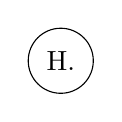
\begin{tikzpicture}[baseline=(n.base)]\node[draw,circle,inner sep=4pt] (n) {H.};\end{tikzpicture}}}}{\margin{\diagram{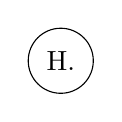
\begin{tikzpicture}[baseline=(n.base)]\node[draw,circle,inner sep=4pt] (n) {H.};\end{tikzpicture}}}}{marginal note placed}{ps_134-3_018-v0012} al model  for a triangulation,  which\var{\inserted{H.}}{\hand{H.}}{insertion}{ps_134-3_018-v0013} Cartan time ago called ``schéma sim%
plicial'' ...) of the two spaces are canonically isomorphic,  because
the ``flags'' of K and $K^{o}$ are the same.  A similar argument due to Quillen
using the nerves shows that for any category K  (not necessarily ordered\unsure{\hand{)}}
K and $K^{o}$ are homotopic,  although\var{\inserted{$\widehat{K}$ and $\widehat{K^{o}}$ are}}{\hand{$\widehat{K}$ and $\widehat{K^{o}}$ are}}{insertion}{ps_134-3_018-v0014} definitely not equivalent i.e. \var{\inserted{not}}{\hand{not}}{insertion}{ps_134-3_018-v0015}
``homeomorphic'' .

To come back to the decreasing cascade of algebraic structures sui-%
table for describing homotopy types,  we could go down one more step
still,  to the category of  maquettes  (Maq) ,  namely sets\var{\inserted{S}}{\hand{S}}{insertion}{ps_134-3_018-v0016} together
with a family\var{\inserted{K}}{\hand{K}}{insertion}{ps_134-3_018-v0017} of finite subsets (the simplices\hand{\illegible{1}} of \var{\over{t}{t}}{\hand{t}}{writing over}{ps_134-3_018-v0018}he set of vertices

%% END SOURCE ps_134-3_018
\ifnum\EditionMode=1
\psapparatusstart
\psentry{ps_134-3_018-v0001}{1}{marginal note placed}{\margin{$\times$}}{\margin{$\times$}}{The marginal material is set at its source-line call; any internal cancellations and replacements are applied in the corrected form.}
\psentry{ps_134-3_018-v0002}{2}{insertion}{\inserted{$\mathcal{T}$}}{\hand{$\mathcal{T}$}}{The handwritten insertion is incorporated at its indicated position; insertion brackets leave the running text.}
\psentry{ps_134-3_018-v0003}{3}{typewriter deletion}{\xout{defines}}{}{The typewriter strikes out this material; it leaves the corrected running text.}
\psentry{ps_134-3_018-v0004}{4}{typewriter deletion}{\xout{as being}}{}{The typewriter strikes out this material; it leaves the corrected running text.}
\psentry{ps_134-3_018-v0005}{5}{writing over}{\over{v}{V}}{\hand{V}}{The superposed handwritten reading replaces the underlying reading.}
\psentry{ps_134-3_018-v0006}{6}{typewriter deletion}{\xout{of all}}{}{The typewriter strikes out this material; it leaves the corrected running text.}
\psentry{ps_134-3_018-v0007}{7}{insertion}{\inserted{on $(K,\mathcal{T})$}}{\hand{on $(K,\mathcal{T})$}}{The handwritten insertion is incorporated at its indicated position; insertion brackets leave the running text.}
\psentry{ps_134-3_018-v0008}{8}{typewriter deletion}{\xout{is just the}}{}{The typewriter strikes out this material; it leaves the corrected running text.}
\psentry{ps_134-3_018-v0009}{9}{insertion}{\inserted{$(K,\mathcal{T})$}}{\hand{$(K,\mathcal{T})$}}{The handwritten insertion is incorporated at its indicated position; insertion brackets leave the running text.}
\psentry{ps_134-3_018-v0010}{10}{writing over}{\over{\unsure{y}}{u}}{\hand{u}}{The superposed handwritten reading replaces the underlying reading.}
\psentry{ps_134-3_018-v0011}{11}{insertion}{\inserted{and}}{\hand{and}}{The handwritten insertion is incorporated at its indicated position; insertion brackets leave the running text.}
\psentry{ps_134-3_018-v0012}{12}{marginal note placed}{\margin{\diagram{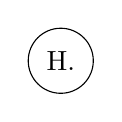
\begin{tikzpicture}[baseline=(n.base)]\node[draw,circle,inner sep=4pt] (n) {H.};\end{tikzpicture}}}}{\margin{\diagram{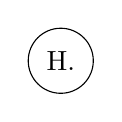
\begin{tikzpicture}[baseline=(n.base)]\node[draw,circle,inner sep=4pt] (n) {H.};\end{tikzpicture}}}}{The marginal material is set at its source-line call; any internal cancellations and replacements are applied in the corrected form.}
\psentry{ps_134-3_018-v0013}{13}{insertion}{\inserted{H.}}{\hand{H.}}{The handwritten insertion is incorporated at its indicated position; insertion brackets leave the running text.}
\psentry{ps_134-3_018-v0014}{14}{insertion}{\inserted{$\widehat{K}$ and $\widehat{K^{o}}$ are}}{\hand{$\widehat{K}$ and $\widehat{K^{o}}$ are}}{The handwritten insertion is incorporated at its indicated position; insertion brackets leave the running text.}
\psentry{ps_134-3_018-v0015}{15}{insertion}{\inserted{not}}{\hand{not}}{The handwritten insertion is incorporated at its indicated position; insertion brackets leave the running text.}
\psentry{ps_134-3_018-v0016}{16}{insertion}{\inserted{S}}{\hand{S}}{The handwritten insertion is incorporated at its indicated position; insertion brackets leave the running text.}
\psentry{ps_134-3_018-v0017}{17}{insertion}{\inserted{K}}{\hand{K}}{The handwritten insertion is incorporated at its indicated position; insertion brackets leave the running text.}
\psentry{ps_134-3_018-v0018}{18}{writing over}{\over{t}{t}}{\hand{t}}{The superposed handwritten reading replaces the underlying reading.}
\psapparatusend
\fi
\pssource{ps_134-3_019}{134-3/19}{https://grothendieck.umontpellier.fr/web/viewer.html?file=../134-3.pdf\#page=20}
\psnumber{ps_134-3_019-v0001}{1}
\psnumber{ps_134-3_019-v0002}{2}
\psnumber{ps_134-3_019-v0003}{3}
\psnumber{ps_134-3_019-v0004}{4}
\psnumber{ps_134-3_019-v0005}{5}
\psnumber{ps_134-3_019-v0006}{6}
\psnumber{ps_134-3_019-v0007}{7}
\psnumber{ps_134-3_019-v0008}{8}
\psnumber{ps_134-3_019-v0009}{9}
\psnumber{ps_134-3_019-v0010}{10}
\psnumber{ps_134-3_019-v0011}{11}
\psnumber{ps_134-3_019-v0012}{12}
\psnumber{ps_134-3_019-v0013}{13}
\psnumber{ps_134-3_019-v0014}{14}
\psnumber{ps_134-3_019-v0015}{15}
%% BEGIN SOURCE ps_134-3_019
% Pursuing Stacks (cotes 134-2 to 134-8): archive cote 134-3, site page 19 (PDF page 20), typescript page 19.
% typescript. Draft compared: ps2.tex:851-922.
% AI-transcribed by Claude Opus 5.5 (claude-opus-5-5, adaptive thinking, effort high), Message Batches API, batch ps1 (msgbatch_01Rv5hCaNTtUt4JHx1yqoHPL), 2026-11-12; image review recorded in records/CHECK_DECISIONS_134_3_4.tsv.
\scanpage{134-3/19}
\mspage{\hand{19}}

S),  such that one-point subsets are simplices and a subset of a simplex
is a simplex.  This category,  via the functor   $(S,K)\hand{\mapsto} K$ ,  is equi-%
valent to the full subcategory of (Ord),  whose objects are those ordered
sets $K$,  such that for every $x\hand{\in}K$,  the set $K_{\hand{\leq}x}$  be isomorphic to the
\var{\margin{\diagram{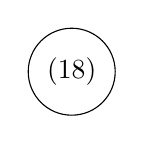
\begin{tikzpicture}[baseline=(n.base)]\node[draw,circle,inner sep=4pt] (n) {(18)};\end{tikzpicture}}}}{\margin{\diagram{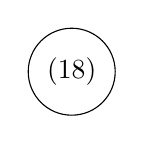
\begin{tikzpicture}[baseline=(n.base)]\node[draw,circle,inner sep=4pt] (n) {(18)};\end{tikzpicture}}}}{marginal note placed}{ps_134-3_019-v0001}ordered set of \var{\xout{finite}}{}{typewriter deletion}{ps_134-3_019-v0002} non empty subsets of some finite set (or ``simplex'').
Here \var{\xout{again}}{}{typewriter deletion}{ps_134-3_019-v0003} the question \var{\xout{arises}}{}{typewriter deletion}{ps_134-3_019-v0004} whether  this category is a model category
in the technical sense \var{\inserted{[of Quillen]}}{\hand{[of Quillen]}}{insertion}{ps_134-3_019-v0005} does'nt really arise\hand{(18)}\hand{,} because this category
does'nt \var{\inserted{even}}{\hand{even}}{insertion}{ps_134-3_019-v0006} admit finite products -  rien à faire !
\var{\margin{\unsure{\unsure{(17)} 5.3. indeed, the notion of a maquette is \uline{not} an algebraic structure species!}}}{\margin{\unsure{\unsure{(17)} 5.3. indeed, the notion of a maquette is \uline{not} an algebraic structure species!}}}{marginal note placed}{ps_134-3_019-v0007}

\var{\over{23}{23}}{\hand{23}}{writing over}{ps_134-3_019-v0008}.  It may be about time to get back to stacks,  still I can't help go-%
ing on pondering about algebraic structures as models for homotopy types.
If we have any algebraic structure species,  giving \var{\inserted{rise to}}{\hand{rise to}}{insertion}{ps_134-3_019-v0009} a category $M$ of
set-theoretic realizations,  the basic question here does'nt seem so
much whether $M$ is a model category for a suitable choice of the three
sets of arrows (fibrations,  cofibrations,  weak equivalences),  but
rather how to define a natural functor
\[ (*) \qquad M \hand{\longrightarrow} (\mathrm{Hot}) \hand{,} \]
where (Hot) is the category of usual homotopy types,  and see whether
via this functor (Hot) can be interpreted as a category of fractions
\hand{(}or ``localization''\hand{)}of $M$  -  namely,  of course,  by the operation of making
invertible those arrows in $M$ which are transformed into isomorphisms
in (Hot).  In any case,  if we have such a natural functor,  the natural
thing to do is to call those arrows ``weak equivalences''.  If we want $M$
\var{\margin{\hand{(9)}}}{\margin{\hand{(9)}}}{marginal note placed}{ps_134-3_019-v0010}to be a category of models,  various examples suggest that the natural
thing again is to take as cofibrations the monomorphisms,\hand{(9)}\hand{,} and then
(expecting that the model categories we are going to meet will be closed
model categories) to define fibrations by the Serre-Quillen lifting pro-%
perty with respect to cofibrations (=monomorphisms) which are weak equi-%
valences.  This being done,  it becomes meaningful to ask if indeed $M$
is a category of models.

Now the reflections of the beginning of today's notes \var{\deleted{p.14-15}}{}{deletion}{ps_134-3_019-v0011} \var{\inserted{section 20}}{\hand{section 20}}{insertion}{ps_134-3_019-v0012}
suggest a rather natural way for describing a functor $(*)$,  which makes
\var{\margin{\diagram{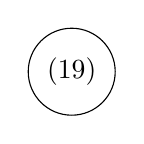
\begin{tikzpicture}[baseline=(n.base)]\node[draw,circle,inner sep=4pt] (n) {(19)};\end{tikzpicture}}}}{\margin{\diagram{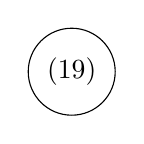
\begin{tikzpicture}[baseline=(n.base)]\node[draw,circle,inner sep=4pt] (n) {(19)};\end{tikzpicture}}}}{marginal note placed}{ps_134-3_019-v0013}sense in fact,  in principle,  for any category $M$,  namely:  endow $M$ with
it's canonical topology (unless a still more natural one appears at hand\hand{(19)}
\var{\margin{$($}}{\margin{$($}}{marginal note placed}{ps_134-3_019-v0014}\var{\margin{\unsure{5.3. the canonical topology is \uline{not} always suitable, see \S 24 below}}}{\margin{\unsure{5.3. the canonical topology is \uline{not} always suitable, see \S 24 below}}}{marginal note placed}{ps_134-3_019-v0015}-  I am not sure there is any better one in the present context),  and
assume that for every  $X\hand{\in}\mathrm{Ob}\,M$ ,  the pro-homotopy type of the induced
site  $M_{/X}$  is essentially constant,  i.e. can be identified with an
object in (Hot) itself.  We then get the functor $(*)$ in an obvious way.
It then becomes meaningful to ask whether this functor is a localization
functor.

When $M$ is defined in terms of an algebraic structure species,  it

%% END SOURCE ps_134-3_019
\ifnum\EditionMode=1
\psapparatusstart
\psentry{ps_134-3_019-v0001}{1}{marginal note placed}{\margin{\diagram{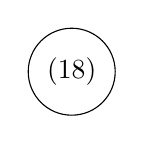
\begin{tikzpicture}[baseline=(n.base)]\node[draw,circle,inner sep=4pt] (n) {(18)};\end{tikzpicture}}}}{\margin{\diagram{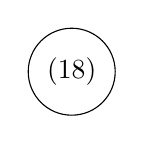
\begin{tikzpicture}[baseline=(n.base)]\node[draw,circle,inner sep=4pt] (n) {(18)};\end{tikzpicture}}}}{The marginal material is set at its source-line call; any internal cancellations and replacements are applied in the corrected form.}
\psentry{ps_134-3_019-v0002}{2}{typewriter deletion}{\xout{finite}}{}{The typewriter strikes out this material; it leaves the corrected running text.}
\psentry{ps_134-3_019-v0003}{3}{typewriter deletion}{\xout{again}}{}{The typewriter strikes out this material; it leaves the corrected running text.}
\psentry{ps_134-3_019-v0004}{4}{typewriter deletion}{\xout{arises}}{}{The typewriter strikes out this material; it leaves the corrected running text.}
\psentry{ps_134-3_019-v0005}{5}{insertion}{\inserted{[of Quillen]}}{\hand{[of Quillen]}}{The handwritten insertion is incorporated at its indicated position; insertion brackets leave the running text.}
\psentry{ps_134-3_019-v0006}{6}{insertion}{\inserted{even}}{\hand{even}}{The handwritten insertion is incorporated at its indicated position; insertion brackets leave the running text.}
\psentry{ps_134-3_019-v0007}{7}{marginal note placed}{\margin{\unsure{\unsure{(17)} 5.3. indeed, the notion of a maquette is \uline{not} an algebraic structure species!}}}{\margin{\unsure{\unsure{(17)} 5.3. indeed, the notion of a maquette is \uline{not} an algebraic structure species!}}}{The marginal material is set at its source-line call; any internal cancellations and replacements are applied in the corrected form.}
\psentry{ps_134-3_019-v0008}{8}{writing over}{\over{23}{23}}{\hand{23}}{The superposed handwritten reading replaces the underlying reading.}
\psentry{ps_134-3_019-v0009}{9}{insertion}{\inserted{rise to}}{\hand{rise to}}{The handwritten insertion is incorporated at its indicated position; insertion brackets leave the running text.}
\psentry{ps_134-3_019-v0010}{10}{marginal note placed}{\margin{\hand{(9)}}}{\margin{\hand{(9)}}}{The marginal material is set at its source-line call; any internal cancellations and replacements are applied in the corrected form.}
\psentry{ps_134-3_019-v0011}{11}{deletion}{\deleted{p.14-15}}{}{The author cancels this material by hand; it leaves the corrected running text.}
\psentry{ps_134-3_019-v0012}{12}{insertion}{\inserted{section 20}}{\hand{section 20}}{The handwritten insertion is incorporated at its indicated position; insertion brackets leave the running text.}
\psentry{ps_134-3_019-v0013}{13}{marginal note placed}{\margin{\diagram{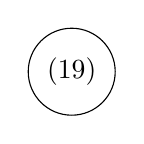
\begin{tikzpicture}[baseline=(n.base)]\node[draw,circle,inner sep=4pt] (n) {(19)};\end{tikzpicture}}}}{\margin{\diagram{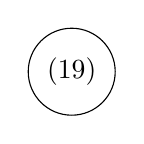
\begin{tikzpicture}[baseline=(n.base)]\node[draw,circle,inner sep=4pt] (n) {(19)};\end{tikzpicture}}}}{The marginal material is set at its source-line call; any internal cancellations and replacements are applied in the corrected form.}
\psentry{ps_134-3_019-v0014}{14}{marginal note placed}{\margin{$($}}{\margin{$($}}{The marginal material is set at its source-line call; any internal cancellations and replacements are applied in the corrected form.}
\psentry{ps_134-3_019-v0015}{15}{marginal note placed}{\margin{\unsure{5.3. the canonical topology is \uline{not} always suitable, see \S 24 below}}}{\margin{\unsure{5.3. the canonical topology is \uline{not} always suitable, see \S 24 below}}}{The marginal material is set at its source-line call; any internal cancellations and replacements are applied in the corrected form.}
\psapparatusend
\fi
\pssource{ps_134-3_020}{134-3/20}{https://grothendieck.umontpellier.fr/web/viewer.html?file=../134-3.pdf\#page=21}
\psnumber{ps_134-3_020-v0001}{1}
\psnumber{ps_134-3_020-v0002}{2}
\psnumber{ps_134-3_020-v0003}{3}
\psnumber{ps_134-3_020-v0004}{4}
\psnumber{ps_134-3_020-v0005}{5}
\psnumber{ps_134-3_020-v0006}{6}
\psnumber{ps_134-3_020-v0007}{7}
\psnumber{ps_134-3_020-v0008}{8}
\psnumber{ps_134-3_020-v0009}{9}
\psnumber{ps_134-3_020-v0010}{10}
\psnumber{ps_134-3_020-v0011}{11}
\psnumber{ps_134-3_020-v0012}{12}
\psnumber{ps_134-3_020-v0013}{13}
%% BEGIN SOURCE ps_134-3_020
% Pursuing Stacks (cotes 134-2 to 134-8): archive cote 134-3, site page 20 (PDF page 21), typescript page 20.
% typescript. Draft compared: ps2.tex:909-968.
% AI-transcribed by Claude Opus 5.5 (claude-opus-5-5, adaptive thinking, effort high), Message Batches API, batch ps1 (msgbatch_01Rv5hCaNTtUt4JHx1yqoHPL), 2026-11-12; image review recorded in records/CHECK_DECISIONS_134_3_4.tsv.
\scanpage{134-3/20}
\mspage{\hand{20}}

admits both types of limits,  without finitesness requirement  -  and
we certainly would expect \var{\inserted[typed]{indeed}}{indeed}{typed insertion}{ps_134-3_020-v0001} at least existence of finite \uline{and} infinite di-%
rect sums in M,  if objects of M were to describe arbitrary homotopy
types.  However,  in view of the special exactness properties of (Hot),
which are by no means autodual,  we will expect moreover direct sums in
M to be ``universal and disjoint'',  in Giraud's sense.  This condition,
which caracterizes to a certain extent categories which at least mildly
resemble or parallel  categories such as (Sets), (Spaces) and similar
categories,whose objects more or less express ``shapes'' -  this condition
at once rules out the majority of the most common algebraic structures,
such as rings,  groups,\var{\xout{and the}}{}{typewriter deletion}{ps_134-3_020-v0002} modules over a ring or anything which
yields for M an abelian category,  etc.  If we describe an algebraic
structure species in terms of its universal realization in a category
stable under finite inverse limits,  then \var{\deleted{a}}{}{deletion}{ps_134-3_020-v0003}\var{\inserted[typed]{such}}{such}{typed insertion}{ps_134-3_020-v0004} structure species can be
viewed as being defined by such a category $\underline{C}$ , and its realizations in
\var{\inserted{any other such $C$ can be interpreted}}{\hand{any other such $C$ can be interpreted}}{insertion}{ps_134-3_020-v0005} \var{\deleted{C}}{}{deletion}{ps_134-3_020-v0006} as the left-exact functors $\underline{C}\hand{\to}C$ (the universal realization of the
structure within $\underline{C}$  corresponding to the identity functor $\underline{C}\hand{\Longrightarrow}\underline{C}$).  In
terms of the dual category $\underline{B}$ ,  associating to every element in
Ob $\underline{B}$  =  Ob $\underline{C}$  the covariant functor $\underline{C}\hand{\to}$(Sets) it represents,  we get
a fully-faithful embedding
\[ \underline{B}\hand{\hookrightarrow} M , \]
by which $\underline{B}$ can be interpreted as the \var{\inserted{category of the}}{\hand{category of the}}{insertion}{ps_134-3_020-v0007} (set-theoretic) realizations of
the given structure  which are of ``finite presentation'' in a suitable
sense (in terms of a given family of generators of $\underline{B}$ namely cogenerators
of $\underline{C}$,  considered as corresponding to the choice of ``base-sets'' for the
given structure species  -  \var{\xout{this}}{}{typewriter deletion}{ps_134-3_020-v0008}\var{\inserted[typed]{such}}{such}{typed insertion}{ps_134-3_020-v0009} choice however being considered as
a convenient way merely to describe the species in concrete terms ...).
\var{\over{I}{I}}{\hand{I}}{writing over}{ps_134-3_020-v0010}f I remember correctly,  M can \var{\over{b}{b}}{\hand{b}}{writing over}{ps_134-3_020-v0011}e deduced from $\underline{B}$,  up to equivalence,
as being merely the category of Ind-objects of $\underline{B}$ ,  i.e. the inclusion
functor above yields an equivalence of categories
\[ \mathrm{Ind}(\underline{B}) \hand{\xrightarrow{\approx}} M , \]
which implies, I guess\var{\xout{\illegible{1}}}{}{typewriter deletion}{ps_134-3_020-v0012},  that the exactness properties of M mainly
reflect those of $\underline{B}$ .  Thus I would expect the condition we want on direct
sums in M to correspond to the same condition for finite direct sums in
$\underline{B}$ ,  not more not less.  Thus the algebraic structure species satisfying
this condition should correspond exactly to small categories $\underline{B}$,  stable
under finite direct limits,  and such that finite sums in $\underline{B}$ are disjoint
and universal.   This condition is presumably necessary,  if we want the
functor (*) from M to Hot  to be defined and to be a localization func-%
tor  -   a condition which it would be nice to understand directly in \var{\xout{te}}{}{typewriter deletion}{ps_134-3_020-v0013}

%% END SOURCE ps_134-3_020
\ifnum\EditionMode=1
\psapparatusstart
\psentry{ps_134-3_020-v0001}{1}{typed insertion}{\inserted[typed]{indeed}}{indeed}{The typed insertion is incorporated at its indicated position; insertion brackets leave the running text.}
\psentry{ps_134-3_020-v0002}{2}{typewriter deletion}{\xout{and the}}{}{The typewriter strikes out this material; it leaves the corrected running text.}
\psentry{ps_134-3_020-v0003}{3}{deletion}{\deleted{a}}{}{The author cancels this material by hand; it leaves the corrected running text.}
\psentry{ps_134-3_020-v0004}{4}{typed insertion}{\inserted[typed]{such}}{such}{The typed insertion is incorporated at its indicated position; insertion brackets leave the running text.}
\psentry{ps_134-3_020-v0005}{5}{insertion}{\inserted{any other such $C$ can be interpreted}}{\hand{any other such $C$ can be interpreted}}{The handwritten insertion is incorporated at its indicated position; insertion brackets leave the running text.}
\psentry{ps_134-3_020-v0006}{6}{deletion}{\deleted{C}}{}{The author cancels this material by hand; it leaves the corrected running text.}
\psentry{ps_134-3_020-v0007}{7}{insertion}{\inserted{category of the}}{\hand{category of the}}{The handwritten insertion is incorporated at its indicated position; insertion brackets leave the running text.}
\psentry{ps_134-3_020-v0008}{8}{typewriter deletion}{\xout{this}}{}{The typewriter strikes out this material; it leaves the corrected running text.}
\psentry{ps_134-3_020-v0009}{9}{typed insertion}{\inserted[typed]{such}}{such}{The typed insertion is incorporated at its indicated position; insertion brackets leave the running text.}
\psentry{ps_134-3_020-v0010}{10}{writing over}{\over{I}{I}}{\hand{I}}{The superposed handwritten reading replaces the underlying reading.}
\psentry{ps_134-3_020-v0011}{11}{writing over}{\over{b}{b}}{\hand{b}}{The superposed handwritten reading replaces the underlying reading.}
\psentry{ps_134-3_020-v0012}{12}{typewriter deletion}{\xout{\illegible{1}}}{}{The typewriter strikes out this material; it leaves the corrected running text.}
\psentry{ps_134-3_020-v0013}{13}{typewriter deletion}{\xout{te}}{}{The typewriter strikes out this material; it leaves the corrected running text.}
\psapparatusend
\fi
\pssource{ps_134-3_021}{134-3/21}{https://grothendieck.umontpellier.fr/web/viewer.html?file=../134-3.pdf\#page=22}
\psnumber{ps_134-3_021-v0001}{1}
\psnumber{ps_134-3_021-v0002}{2}
\psnumber{ps_134-3_021-v0003}{3}
\psnumber{ps_134-3_021-v0004}{4}
\psnumber{ps_134-3_021-v0005}{5}
\psnumber{ps_134-3_021-v0006}{6}
\psnumber{ps_134-3_021-v0007}{7}
\psnumber{ps_134-3_021-v0008}{8}
\psnumber{ps_134-3_021-v0009}{9}
\psnumber{ps_134-3_021-v0010}{10}
\psnumber{ps_134-3_021-v0011}{11}
\psnumber{ps_134-3_021-v0012}{12}
\psnumber{ps_134-3_021-v0013}{13}
\psnumber{ps_134-3_021-v0014}{14}
\psnumber{ps_134-3_021-v0015}{15}
\psnumber{ps_134-3_021-v0016}{16}
\psnumber{ps_134-3_021-v0017}{17}
\psnumber{ps_134-3_021-v0018}{18}
\psnumber{ps_134-3_021-v0019}{19}
\psnumber{ps_134-3_021-v0020}{20}
\psnumber{ps_134-3_021-v0021}{21}
\psnumber{ps_134-3_021-v0022}{22}
\psnumber{ps_134-3_021-v0023}{23}
\psnumber{ps_134-3_021-v0024}{24}
\psnumber{ps_134-3_021-v0025}{25}
\psnumber{ps_134-3_021-v0026}{26}
%% BEGIN SOURCE ps_134-3_021
% Pursuing Stacks (cotes 134-2 to 134-8): archive cote 134-3, site page 21 (PDF page 22), typescript page 21.
% typescript. Draft compared: ps2.tex:955-1024.
% AI-transcribed by Claude Opus 5.5 (claude-opus-5-5, adaptive thinking, effort high), Message Batches API, batch ps1 (msgbatch_01Rv5hCaNTtUt4JHx1yqoHPL), 2026-11-12; image review recorded in records/CHECK_DECISIONS_134_3_4.tsv.
\scanpage{134-3/21}
\mspage{\hand{21}}

terms of $\underline{B}$ , and (presumably) in terms of the canonical topology\var{\inserted{(19)}}{\hand{(19)}}{insertion}{ps_134-3_021-v0001} of $\underline{B}$ ,
which should give rise to a\var{\xout{\unsure{xxxqui}}}{}{typewriter deletion}{ps_134-3_021-v0002} localization functor
\[ \underline{B} \hand{\longrightarrow} (\mathrm{Hot})_{\mathrm{f.t.}} \quad , \]
where the subscript f.t. means ``finite type'' - granting that the notion
of homotopy types of finite type (presumably the same as homotopy types
of finite triangulations,\var{\inserted{or}}{\hand{or}}{insertion}{ps_134-3_021-v0003} of\var{\inserted{``finite''}}{\hand{``finite''}}{insertion}{ps_134-3_021-v0004} C.W. spaces) is a well defined notion\var{\inserted{(20)}}{\hand{(20)}}{insertion}{ps_134-3_021-v0005}.
As usual, it is in $\underline{B}$ , not in $\underline{C}$ , that geometrical constructions
take place which make sense for topological intuition. More specifical-%
ly, it seems that in the cases met\var{\inserted{with}}{\hand{with}}{insertion}{ps_134-3_021-v0006} so far, there \uline{are} indeed privileged
base-sets for the structure species considered (such as the``components''
of a semi\var{\xout{s}}{}{typewriter deletion}{ps_134-3_021-v0007}simplicial of cubical complex, or of a stack, etc ), indexed
by the\var{\inserted[typed]{natural}}{natural}{typed insertion}{ps_134-3_021-v0008} integers or n-tupels of such integers, and which``correspond'' to
topological cells of various dimensions, \var{\deleted{the}}{}{deletion}{ps_134-3_021-v0009}\var{\inserted{Moreover,}}{\hand{Moreover,}}{insertion}{ps_134-3_021-v0010} some of the basic structu-%
ral\var{\inserted{monomorphic}}{\hand{monomorphic}}{insertion}{ps_134-3_021-v0011} maps between these\var{\inserted{objects of $\underline{B}$}}{\hand{objects of $\underline{B}$}}{insertion}{ps_134-3_021-v0012} defin\var{\over{ing}{e}}{\hand{e}}{writing over}{ps_134-3_021-v0013} cellular decompositions of the\var{\inserted[typed]{topological}}{topological}{typed insertion}{ps_134-3_021-v0014} spheres
bounding these topological cells. These objects and ``boundary\hand{*} maps''
between them \var{\deleted{\xout{form}}}{}{deletion}{ps_134-3_021-v0015}\var{\inserted[typed]{define}}{define}{typed insertion}{ps_134-3_021-v0016} a (non full, in general) subcategory of $\underline{B}$ , say $\underline{B}_{\mathrm{oo}}$ ,
which looks like the core of the category $\underline{B}$, from which the topological
significance of $\underline{B}$ is springing. It is in terms of $\underline{B}_{\mathrm{oo}}$ that the ``corres-%
pondance '' \hand{(}vaguely referred to above\hand{)} with topological cells\var{\inserted[typed]{and spheres}}{and spheres}{typed insertion}{ps_134-3_021-v0017} takes a
precise meaning. Namely, associating to any object of $\underline{B}_{\mathrm{oo}}$ the ordered
set of its subobjects (within $\underline{B}_{\mathrm{oo}}$ of course, not $\underline{B}$ ), the \var{\xout{conicalx}}{}{typewriter deletion}{ps_134-3_021-v0018}
(stratified) topological realization of this ordered set is a cell, and
the \var{\xout{union}}{}{typewriter deletion}{ps_134-3_021-v0019}\var{\inserted[typed]{family}}{family}{typed insertion}{ps_134-3_021-v0020} of \var{\deleted{\xout{the}}}{}{deletion}{ps_134-3_021-v0021} subcells of smaller dimension (namely different from
the given one) is a cellular subdivision of the\var{\inserted[typed]{sphere}}{sphere}{typed insertion}{ps_134-3_021-v0022} bounding th\var{\over{e}{is}}{\hand{is}}{writing over}{ps_134-3_021-v0023} cell\var{\inserted{(21)}}{\hand{(21)}}{insertion}{ps_134-3_021-v0024}.

\var{\over{\unsure{4}}{7}}{\hand{7}}{writing over}{ps_134-3_021-v0025}.3.
\var{\over{21}{24}}{\hand{24}}{writing over}{ps_134-3_021-v0026}. Yesterday there occured to me a big``étourderie'' again of the day
before, in connection with a reflection on a suitable ``natural'' site
structure on the category (Cat) - namely when asserting that for a
family of morphisms i.e. functors in (Cat)
\[ (*) \qquad A_i \hand{\longrightarrow} A \ , \]
in order for the corresponding family to be ``covering'' namely epimorphic
in the category (a topos, as a matter of fact) (Ss sets), namely for
the corresponding families of mappings of sets
\[ (**) \qquad \mathrm{Fl}_n(A_i) \hand{\longrightarrow} \mathrm{Fl}_n(A) \]
to be epimorphic, it was sufficient that this condition be satisfied
for n=2 (which, according to Giraud, just means that the family (*)
is covering for the canonical topology of (Cat)). This is obviously
false - morally, it would mean that an n-simplex is ``covered'' in a
reasonable sense by it's sub-2-simplices, which is pretty absurd. To

%% END SOURCE ps_134-3_021
\ifnum\EditionMode=1
\psapparatusstart
\psentry{ps_134-3_021-v0001}{1}{insertion}{\inserted{(19)}}{\hand{(19)}}{The handwritten insertion is incorporated at its indicated position; insertion brackets leave the running text.}
\psentry{ps_134-3_021-v0002}{2}{typewriter deletion}{\xout{\unsure{xxxqui}}}{}{The typewriter strikes out this material; it leaves the corrected running text.}
\psentry{ps_134-3_021-v0003}{3}{insertion}{\inserted{or}}{\hand{or}}{The handwritten insertion is incorporated at its indicated position; insertion brackets leave the running text.}
\psentry{ps_134-3_021-v0004}{4}{insertion}{\inserted{``finite''}}{\hand{``finite''}}{The handwritten insertion is incorporated at its indicated position; insertion brackets leave the running text.}
\psentry{ps_134-3_021-v0005}{5}{insertion}{\inserted{(20)}}{\hand{(20)}}{The handwritten insertion is incorporated at its indicated position; insertion brackets leave the running text.}
\psentry{ps_134-3_021-v0006}{6}{insertion}{\inserted{with}}{\hand{with}}{The handwritten insertion is incorporated at its indicated position; insertion brackets leave the running text.}
\psentry{ps_134-3_021-v0007}{7}{typewriter deletion}{\xout{s}}{}{The typewriter strikes out this material; it leaves the corrected running text.}
\psentry{ps_134-3_021-v0008}{8}{typed insertion}{\inserted[typed]{natural}}{natural}{The typed insertion is incorporated at its indicated position; insertion brackets leave the running text.}
\psentry{ps_134-3_021-v0009}{9}{deletion}{\deleted{the}}{}{The author cancels this material by hand; it leaves the corrected running text.}
\psentry{ps_134-3_021-v0010}{10}{insertion}{\inserted{Moreover,}}{\hand{Moreover,}}{The handwritten insertion is incorporated at its indicated position; insertion brackets leave the running text.}
\psentry{ps_134-3_021-v0011}{11}{insertion}{\inserted{monomorphic}}{\hand{monomorphic}}{The handwritten insertion is incorporated at its indicated position; insertion brackets leave the running text.}
\psentry{ps_134-3_021-v0012}{12}{insertion}{\inserted{objects of $\underline{B}$}}{\hand{objects of $\underline{B}$}}{The handwritten insertion is incorporated at its indicated position; insertion brackets leave the running text.}
\psentry{ps_134-3_021-v0013}{13}{writing over}{\over{ing}{e}}{\hand{e}}{The superposed handwritten reading replaces the underlying reading.}
\psentry{ps_134-3_021-v0014}{14}{typed insertion}{\inserted[typed]{topological}}{topological}{The typed insertion is incorporated at its indicated position; insertion brackets leave the running text.}
\psentry{ps_134-3_021-v0015}{15}{deletion}{\deleted{\xout{form}}}{}{The author cancels this material by hand; it leaves the corrected running text.}
\psentry{ps_134-3_021-v0016}{16}{typed insertion}{\inserted[typed]{define}}{define}{The typed insertion is incorporated at its indicated position; insertion brackets leave the running text.}
\psentry{ps_134-3_021-v0017}{17}{typed insertion}{\inserted[typed]{and spheres}}{and spheres}{The typed insertion is incorporated at its indicated position; insertion brackets leave the running text.}
\psentry{ps_134-3_021-v0018}{18}{typewriter deletion}{\xout{conicalx}}{}{The typewriter strikes out this material; it leaves the corrected running text.}
\psentry{ps_134-3_021-v0019}{19}{typewriter deletion}{\xout{union}}{}{The typewriter strikes out this material; it leaves the corrected running text.}
\psentry{ps_134-3_021-v0020}{20}{typed insertion}{\inserted[typed]{family}}{family}{The typed insertion is incorporated at its indicated position; insertion brackets leave the running text.}
\psentry{ps_134-3_021-v0021}{21}{deletion}{\deleted{\xout{the}}}{}{The author cancels this material by hand; it leaves the corrected running text.}
\psentry{ps_134-3_021-v0022}{22}{typed insertion}{\inserted[typed]{sphere}}{sphere}{The typed insertion is incorporated at its indicated position; insertion brackets leave the running text.}
\psentry{ps_134-3_021-v0023}{23}{writing over}{\over{e}{is}}{\hand{is}}{The superposed handwritten reading replaces the underlying reading.}
\psentry{ps_134-3_021-v0024}{24}{insertion}{\inserted{(21)}}{\hand{(21)}}{The handwritten insertion is incorporated at its indicated position; insertion brackets leave the running text.}
\psentry{ps_134-3_021-v0025}{25}{writing over}{\over{\unsure{4}}{7}}{\hand{7}}{The superposed handwritten reading replaces the underlying reading.}
\psentry{ps_134-3_021-v0026}{26}{writing over}{\over{21}{24}}{\hand{24}}{The superposed handwritten reading replaces the underlying reading.}
\psapparatusend
\fi
\pssource{ps_134-3_022}{134-3/22}{https://grothendieck.umontpellier.fr/web/viewer.html?file=../134-3.pdf\#page=23}
\psnumber{ps_134-3_022-v0001}{1}
\psnumber{ps_134-3_022-v0002}{2}
\psnumber{ps_134-3_022-v0003}{3}
\psnumber{ps_134-3_022-v0004}{4}
\psnumber{ps_134-3_022-v0005}{5}
\psnumber{ps_134-3_022-v0006}{6}
\psnumber{ps_134-3_022-v0007}{7}
\psnumber{ps_134-3_022-v0008}{8}
\psnumber{ps_134-3_022-v0009}{9}
\psnumber{ps_134-3_022-v0010}{10}
\psnumber{ps_134-3_022-v0011}{11}
%% BEGIN SOURCE ps_134-3_022
% Pursuing Stacks (cotes 134-2 to 134-8): archive cote 134-3, site page 22 (PDF page 23), typescript page 22.
% typescript. Draft compared: ps2.tex:1010-1069.
% AI-transcribed by Claude Opus 5.5 (claude-opus-5-5, adaptive thinking, effort high), Message Batches API, batch ps1 (msgbatch_01Rv5hCaNTtUt4JHx1yqoHPL), 2026-11-12; image review recorded in records/CHECK_DECISIONS_134_3_4.tsv.
\scanpage{134-3/22}
\mspage{\hand{22}}
give specific positive statements along these lines, let's\var{\inserted[typed]{for any $N\hand{\in}\underline{N}$,}}{for any $N\hand{\in}\underline{N}$,}{typed insertion}{ps_134-3_022-v0001}denote
by $T_N$ the topology on (Cat) for which a family (*) is covering i\var{\over{s}{ff}}{\hand{ff}}{writing over}{ps_134-3_022-v0002}
the families (**) are for $n\hand{\leqslant} N$ - which means also that the correspon-%
ding family of N-truncated nerves
\[ \mathrm{Nerve}(A_i)\hand{[}N\hand{]} \hand{\longrightarrow} \mathrm{Nerve}(A)\hand{[}N\hand{]} \]
is epimorphic. For N=1, this means that the family is \hand{``}universally
epimorphic\hand{''}, for N=2, that it is \var{\deleted{\unsure{it is|it as}}}{}{deletion}{ps_134-3_022-v0003}\hand{``}universally effectively epimor-%
phic\hand{''}i.e. covering for the canonical topology of (Cat) (Giraud, loc.
cit. page 28). It turns out that this decreasing sequence of topologies
on (Cat) is strictly decreasing - as a matter of fact, denoting by
$\hand{\Delta[}N\hand{]}$ the category of \var{\inserted[typed]{standart ordered}}{standart ordered}{typed insertion}{ps_134-3_022-v0004}\var{\xout{\illegible{1}}}{}{typewriter deletion}{ps_134-3_022-v0005}simplices of dimension $\hand{\leqslant} N$, and using the
inclusions
\[ \hand{\Delta[}N\hand{]\hookrightarrow}(\mathrm{Cat})\hand{\hookrightarrow\Delta}(N)\hand{^{\wedge}} \]
(for $N\hand{\geqslant}2$ say), an immediate application of the ``comparison lemma'' for
sites shows that we have an equivalence
\[ ((\mathrm{Cat}),T_N)\hand{^{\sim}\simeq\Delta[}N\hand{]^{\wedge}}, \]
and hence, for any object A in (Cat) namely any category A , we get
an equivalence
\[ ((\mathrm{Cat}),T_N)_{/A}\hand{)^{\sim}\simeq}(\hand{\Delta}(N)_{/A})\hand{^{\wedge}} \quad , \]
and hence the homotopy type of the first hand member is\var{\inserted{\uline{not}}}{\hand{\uline{not}}}{insertion}{ps_134-3_022-v0006} described by and
equivalent to the homotopy type of the whole Nerve(A) object, but
rather by its N-skeleton, which has the same homotopy and cohomology
invariants in\var{\inserted[typed]{dimension}}{dimension}{typed insertion}{ps_134-3_022-v0007} \var{\xout{degrees}}{}{typewriter deletion}{ps_134-3_022-v0008} $\hand{\leqslant} N$, but by no means for higher dimensions. This
shows that among the topologies $T_N$ , none is suitable for recovering
the homotopy type of objects of (Cat) in the way contemplated two days
ago (page 15); \var{\deleted{but}}{}{deletion}{ps_134-3_022-v0009} the one topology which \uline{is} suitable is the one which
may be denoted by $T_{\infty}$ , and which \var{\xout{wa}}{}{typewriter deletion}{ps_134-3_022-v0010}is the one indeed which I first con-%
templated (page 14), before the mistaken idea occured to me that it was
the same as the canonical topology.

A very similar mistake occured earlier, when I surmised that the\var{\inserted[typed]{left}}{left}{typed insertion}{ps_134-3_022-v0011}
adjoint functor N' to the inclusion or Nerve functor N from (Cat)
to (Ss sets) $=\hand{\Delta^{\wedge}}$ had the property that for any object K in (Ss sets),
K and N'(K) had same homotopy type. Looking up yesterday the descripti-%
on in Gabriel-Zisman of this functor, this recalled to my mind that
it factors (via the natural restriction functor) through the category
$(\hand{\Delta}[2])^{\wedge}$ , hence any morphism $K\hand{\longrightarrow}K'$ inducing an isomorphism on the
2-skeletons (which by no means implies that it is a homotopy equivalen-%
ce) induces an isomorphism $N'(K)\hand{\xrightarrow{\sim}}N'(K')$, and a fortiori a homotopy
equivalence. This shows that, even if it should be true that (Cat) is

%% END SOURCE ps_134-3_022
\ifnum\EditionMode=1
\psapparatusstart
\psentry{ps_134-3_022-v0001}{1}{typed insertion}{\inserted[typed]{for any $N\hand{\in}\underline{N}$,}}{for any $N\hand{\in}\underline{N}$,}{The typed insertion is incorporated at its indicated position; insertion brackets leave the running text.}
\psentry{ps_134-3_022-v0002}{2}{writing over}{\over{s}{ff}}{\hand{ff}}{The superposed handwritten reading replaces the underlying reading.}
\psentry{ps_134-3_022-v0003}{3}{deletion}{\deleted{\unsure{it is|it as}}}{}{The author cancels this material by hand; it leaves the corrected running text.}
\psentry{ps_134-3_022-v0004}{4}{typed insertion}{\inserted[typed]{standart ordered}}{standart ordered}{The typed insertion is incorporated at its indicated position; insertion brackets leave the running text.}
\psentry{ps_134-3_022-v0005}{5}{typewriter deletion}{\xout{\illegible{1}}}{}{The typewriter strikes out this material; it leaves the corrected running text.}
\psentry{ps_134-3_022-v0006}{6}{insertion}{\inserted{\uline{not}}}{\hand{\uline{not}}}{The handwritten insertion is incorporated at its indicated position; insertion brackets leave the running text.}
\psentry{ps_134-3_022-v0007}{7}{typed insertion}{\inserted[typed]{dimension}}{dimension}{The typed insertion is incorporated at its indicated position; insertion brackets leave the running text.}
\psentry{ps_134-3_022-v0008}{8}{typewriter deletion}{\xout{degrees}}{}{The typewriter strikes out this material; it leaves the corrected running text.}
\psentry{ps_134-3_022-v0009}{9}{deletion}{\deleted{but}}{}{The author cancels this material by hand; it leaves the corrected running text.}
\psentry{ps_134-3_022-v0010}{10}{typewriter deletion}{\xout{wa}}{}{The typewriter strikes out this material; it leaves the corrected running text.}
\psentry{ps_134-3_022-v0011}{11}{typed insertion}{\inserted[typed]{left}}{left}{The typed insertion is incorporated at its indicated position; insertion brackets leave the running text.}
\psapparatusend
\fi
\pssource{ps_134-3_023}{134-3/23}{https://grothendieck.umontpellier.fr/web/viewer.html?file=../134-3.pdf\#page=24}
\psnumber{ps_134-3_023-v0001}{1}
\psnumber{ps_134-3_023-v0002}{2}
\psnumber{ps_134-3_023-v0003}{3}
\psnumber{ps_134-3_023-v0004}{4}
\psnumber{ps_134-3_023-v0005}{5}
\psnumber{ps_134-3_023-v0006}{6}
\psnumber{ps_134-3_023-v0007}{7}
\psnumber{ps_134-3_023-v0008}{8}
\psnumber{ps_134-3_023-v0009}{9}
\psnumber{ps_134-3_023-v0010}{10}
\psnumber{ps_134-3_023-v0011}{11}
\psnumber{ps_134-3_023-v0012}{12}
\psnumber{ps_134-3_023-v0013}{13}
\psnumber{ps_134-3_023-v0014}{14}
\psnumber{ps_134-3_023-v0015}{15}
%% BEGIN SOURCE ps_134-3_023
% Pursuing Stacks (cotes 134-2 to 134-8): archive cote 134-3, site page 23 (PDF page 24), typescript page 23.
% typescript. Draft compared: ps2.tex:1055-1122.
% AI-transcribed by Claude Opus 5.5 (claude-opus-5-5, adaptive thinking, effort high), Message Batches API, batch ps1 (msgbatch_01Rv5hCaNTtUt4JHx1yqoHPL), 2026-11-12; image review recorded in records/CHECK_DECISIONS_134_3_4.tsv.
\scanpage{134-3/23}
\mspage{\hand{23}}
a model category in Quillen's sense,  the situation with the inclusion
functor
\[ N:(Cat)\hand{\longrightarrow} (Ss sets) \]
and the left adjoint functor N'  is by no means the one of Quillen\hand{'}s
comparison theorem,  where the two functors play\var{\xout{ed}}{}{typewriter deletion}{ps_134-3_023-v0001} mutually dual roles
and both induce equivalences on the corresponding localized homotopical
categories.  Here \uline{only} N,  \uline{not} N',  \uline{induces such equivalence}.  This is
analoguous to the situation,  already note\var{\over{\unsure{s}}{d}}{\hand{d}}{writing over}{ps_134-3_023-v0002} before,  of the inclusion
functors
\[ (Preord)\hand{\hookrightarrow} (Cat) \qquad or \qquad (Ord)\hand{\hookrightarrow} (Cat) \quad , \]
which \var{\inserted{[presumably]}}{\hand{[presumably]}}{insertion}{ps_134-3_023-v0003} by localization induce equivalences on the associated homotopy
categories,  but the left adjoint functors do not share this property.

The topology $T_\infty$  just considered on (Cat) as a ``suitable'' topology
for describing homotopy types of objects of (Cat),  was\hand{|}of course direct-%
ly inspired by the semi-simplicial approach to homotopy types,  via
simplicial complexes  namely via the two associated inclusion functors
\[ \hand{\Delta} \hand{\hookrightarrow} (Cat)\hand{\hookrightarrow} \hand{\Delta^{\wedge}} , \]
the second functor associating to every category A the ``complex'' of it's
``simplicial diagrams''  $a_o\hand{\longrightarrow} a_1\hand{\longrightarrow} \;\ldots\hand{\longrightarrow} a_n$ .  If we had been working
\var{\xout{rather}}{}{typewriter deletion}{ps_134-3_023-v0004} with  cubical complexes rather than ss ones for describing homoto
-py types,  this would give rise similarly to two functors
\[ \hand{\square} \hand{\hookrightarrow} (Cat)\hand{\hookrightarrow} \hand{\square^{\wedge}} , \]
where $\hand{\square}$ is the category of``standar\var{\over{t}{d}}{\hand{d}}{writing over}{ps_134-3_023-v0005} cubes'' and face and degeneracy
maps between them,  and where the second\hand{|}inclusion associates to every
category A the cubical complex of it's  ``cubical diagrams'',  namely \var{\inserted[typed]{commutative}}{commutative}{typed insertion}{ps_134-3_023-v0006}
diagrams in A modelled after the diagram types $\hand{\square}_n\hand{[}1\hand{]}$ ,  the 1-skeleton
of the standart n-cubes $\hand{\square}_n$ , with suitable orientations on it's edges
(indicative of the direction of corresponding arrows in A).  The natural
idea \var{\over{\xout{here}}{now}}{\hand{now}}{writing over}{ps_134-3_023-v0007} would be to endow (Cat) with the \var{\over{category}{topology}}{\hand{topology}}{writing over}{ps_134-3_023-v0008}, $T'_\infty$ say,  induced
by $\hand{\square^{\wedge}}$,  namely call a family (*)  covering iff for every $n\hand{\in} \underline{N}$,  the
corresponding family  of \var{\xout{set}}{}{typewriter deletion}{ps_134-3_023-v0009} maps of sets
\[ Cub_n(A_i)\hand{\longrightarrow} \hand{C}ub_n(A) \]
is epimorphic.   This \var{\xout{category}}{}{typewriter deletion}{ps_134-3_023-v0010} topology appears to be \var{\xout{finer}}{}{typewriter deletion}{ps_134-3_023-v0011}\var{\inserted[typed]{coarser}}{coarser}{typed insertion}{ps_134-3_023-v0012} than $T_\infty$ \var{\xout{,}}{}{typewriter deletion}{ps_134-3_023-v0013}
\var{\inserted[typed]{(i.e. there are less covering families),}}{(i.e. there are less covering families),}{typed insertion}{ps_134-3_023-v0014}
and the comparison lemma gives now the equivalence
\[ ((Cat),T'_\infty)\hand{^{\sim}} \hand{\simeq} \hand{\square^{\wedge}} , \]
which shows that definitely the topology is \uline{strictly} coarser than $T_\infty$ ,
as it gives rise to a non-equivalent topos,  $\hand{\square^{\wedge}}$ instead of $\hand{\Delta^{\wedge}}$.

T\var{\over{h}{h}}{\hand{h}}{writing over}{ps_134-3_023-v0015}ese reflections convince me  1)  there are indeed topologies
on (Cat),  suit\unsure{able for} describing the natural homotopy types of ob-%
jects of (Cat) namely of categories,  and  2)  that there is definitely

%% END SOURCE ps_134-3_023
\ifnum\EditionMode=1
\psapparatusstart
\psentry{ps_134-3_023-v0001}{1}{typewriter deletion}{\xout{ed}}{}{The typewriter strikes out this material; it leaves the corrected running text.}
\psentry{ps_134-3_023-v0002}{2}{writing over}{\over{\unsure{s}}{d}}{\hand{d}}{The superposed handwritten reading replaces the underlying reading.}
\psentry{ps_134-3_023-v0003}{3}{insertion}{\inserted{[presumably]}}{\hand{[presumably]}}{The handwritten insertion is incorporated at its indicated position; insertion brackets leave the running text.}
\psentry{ps_134-3_023-v0004}{4}{typewriter deletion}{\xout{rather}}{}{The typewriter strikes out this material; it leaves the corrected running text.}
\psentry{ps_134-3_023-v0005}{5}{writing over}{\over{t}{d}}{\hand{d}}{The superposed handwritten reading replaces the underlying reading.}
\psentry{ps_134-3_023-v0006}{6}{typed insertion}{\inserted[typed]{commutative}}{commutative}{The typed insertion is incorporated at its indicated position; insertion brackets leave the running text.}
\psentry{ps_134-3_023-v0007}{7}{writing over}{\over{\xout{here}}{now}}{\hand{now}}{The superposed handwritten reading replaces the underlying reading.}
\psentry{ps_134-3_023-v0008}{8}{writing over}{\over{category}{topology}}{\hand{topology}}{The superposed handwritten reading replaces the underlying reading.}
\psentry{ps_134-3_023-v0009}{9}{typewriter deletion}{\xout{set}}{}{The typewriter strikes out this material; it leaves the corrected running text.}
\psentry{ps_134-3_023-v0010}{10}{typewriter deletion}{\xout{category}}{}{The typewriter strikes out this material; it leaves the corrected running text.}
\psentry{ps_134-3_023-v0011}{11}{typewriter deletion}{\xout{finer}}{}{The typewriter strikes out this material; it leaves the corrected running text.}
\psentry{ps_134-3_023-v0012}{12}{typed insertion}{\inserted[typed]{coarser}}{coarser}{The typed insertion is incorporated at its indicated position; insertion brackets leave the running text.}
\psentry{ps_134-3_023-v0013}{13}{typewriter deletion}{\xout{,}}{}{The typewriter strikes out this material; it leaves the corrected running text.}
\psentry{ps_134-3_023-v0014}{14}{typed insertion}{\inserted[typed]{(i.e. there are less covering families),}}{(i.e. there are less covering families),}{The typed insertion is incorporated at its indicated position; insertion brackets leave the running text.}
\psentry{ps_134-3_023-v0015}{15}{writing over}{\over{h}{h}}{\hand{h}}{The superposed handwritten reading replaces the underlying reading.}
\psapparatusend
\fi
\pssource{ps_134-3_024}{134-3/24}{https://grothendieck.umontpellier.fr/web/viewer.html?file=../134-3.pdf\#page=25}
\psnumber{ps_134-3_024-v0001}{1}
\psnumber{ps_134-3_024-v0002}{2}
\psnumber{ps_134-3_024-v0003}{3}
\psnumber{ps_134-3_024-v0004}{4}
\psnumber{ps_134-3_024-v0005}{5}
\psnumber{ps_134-3_024-v0006}{6}
\psnumber{ps_134-3_024-v0007}{7}
\psnumber{ps_134-3_024-v0008}{8}
\psnumber{ps_134-3_024-v0009}{9}
\psnumber{ps_134-3_024-v0010}{10}
\psnumber{ps_134-3_024-v0011}{11}
\psnumber{ps_134-3_024-v0012}{12}
\psnumber{ps_134-3_024-v0013}{13}
\psnumber{ps_134-3_024-v0014}{14}
\psnumber{ps_134-3_024-v0015}{15}
\psnumber{ps_134-3_024-v0016}{16}
\psnumber{ps_134-3_024-v0017}{17}
\psnumber{ps_134-3_024-v0018}{18}
\psnumber{ps_134-3_024-v0019}{19}
\psnumber{ps_134-3_024-v0020}{20}
\psnumber{ps_134-3_024-v0021}{21}
\psnumber{ps_134-3_024-v0022}{22}
\psnumber{ps_134-3_024-v0023}{23}
\psnumber{ps_134-3_024-v0024}{24}
\psnumber{ps_134-3_024-v0025}{25}
\psnumber{ps_134-3_024-v0026}{26}
\psnumber{ps_134-3_024-v0027}{27}
\psnumber{ps_134-3_024-v0028}{28}
%% BEGIN SOURCE ps_134-3_024
% Pursuing Stacks (cotes 134-2 to 134-8): archive cote 134-3, site page 24 (PDF page 25), typescript page 24.
% typescript. Draft compared: ps2.tex:1106-1172.
% AI-transcribed by Claude Opus 5.5 (claude-opus-5-5, adaptive thinking, effort high), Message Batches API, batch pilot (msgbatch_0189Nhf1xB615YWnztubtLfc), 2026-11-12; image review recorded in records/CHECK_DECISIONS_134_3_4.tsv.
\scanpage{134-3/24}
\mspage{24}
no privileged choice for such topology.  We just described two such,
but using \var{\xout{xx}}{}{typewriter deletion}{ps_134-3_024-v0001} multicomplexes (cubical or semisimplicial) rather than
\var{\margin{\diagram{\begin{tikzpicture}[x=1cm,y=1cm]\draw[->] (0.35,0)--(0,0)--(0,0.8);\end{tikzpicture}}}}{\margin{\diagram{\begin{tikzpicture}[x=1cm,y=1cm]\draw[->] (0.35,0)--(0,0)--(0,0.8);\end{tikzpicture}}}}{marginal note placed}{ps_134-3_024-v0002}simple complexes should give us infinitely \var{\inserted[typed]{many}}{many}{typed insertion}{ps_134-3_024-v0003} others  just as suitable,
and I suspect \var{\xout{that}}{}{typewriter deletion}{ps_134-3_024-v0004} now that there must be a big lot more of them still !

\var{\margin{\diagram{\begin{tikzpicture}[x=1cm,y=1cm]\draw[->] (0.35,0.8)--(0,0.8)--(0,0);\end{tikzpicture}}}}{\margin{\diagram{\begin{tikzpicture}[x=1cm,y=1cm]\draw[->] (0.35,0.8)--(0,0.8)--(0,0);\end{tikzpicture}}}}{marginal note placed}{ps_134-3_024-v0005}\var{\over{\illegible{1}}{25}}{\hand{25}}{writing over}{ps_134-3_024-v0006}.  A fortiori,  coming back to the intriguing question of \var{\xout{which}}{}{typewriter deletion}{ps_134-3_024-v0007} carac-%
terizing the algebraic structure species suitable for describing homoto-%
py types in the usual homotopy category (Hot),  \var{\xout{if M is the}}{}{typewriter deletion}{ps_134-3_024-v0008} and for
recovering (Hot) as a category of fractions of the category M of all
set-theoretic re\var{\xout{a}}{}{typewriter deletion}{ps_134-3_024-v0009}alizations of this species,  it becomes clear now that
we cannot hope reasonably for a ``natural'' topology on M,  distinguished
among all others,  giving rise to the wished-for functor
\[ (*) \qquad M \hand{\to} (\mathrm{Hot}) \]
in the way contemplated earlier (\var{\deleted{page 19 ff}}{}{deletion}{ps_134-3_024-v0010}\var{\inserted{section 23}}{\hand{section 23}}{insertion}{ps_134-3_024-v0011}).  Here it occu\var{\over{s}{r}}{\hand{r}}{writing over}{ps_134-3_024-v0012}s to me
that anyhow,  if concerned mainly with defining the functor (*),  we
should consider that two topologies T,T' on M such that $T \hand{\geqslant} T'$  and
hence giving rise to a morphism of topoi
\[ (**) \qquad M_T^{\hand{\sim}} \hand{\to} M_{T'}^{\hand{\sim}} \]
(the \var{\deleted{inverse}}{}{deletion}{ps_134-3_024-v0013}\var{\inserted{direct}}{\hand{direct}}{insertion}{ps_134-3_024-v0014} image functor associated to this morphism being the natural
inclusion functor\var{\xout{s}}{}{typewriter deletion}{ps_134-3_024-v0015}\hand{,} when considering T\var{\deleted{'}}{}{deletion}{ps_134-3_024-v0016}-sheaves as particular cases of
T\hand{'}-sheaves) are ``\uline{equivalent}''  -  maybe we should rather say ``\uline{Hot-equiva-}%
\uline{lent}'' -  if for any  object A in M,  the induced morphism
\var{\margin{\deleted{\illegible{1}}}}{\margin{}}{marginal note placed}{ps_134-3_024-v0017}
\[ (M_T^{\hand{\sim}})_{/A} \hand{\to} (M_{T'}^{\hand{\sim}})_{/A} \]
\var{\margin{\deleted{\illegible{1}}}}{\margin{}}{marginal note placed}{ps_134-3_024-v0018}
is a homotopy equivalence.  This can be viewed as an intrinsic property
of the morphism of topoi (**), of a type rather familiar I guess to
people used to the dial\var{\deleted{\unsure{l}}}{}{deletion}{ps_134-3_024-v0019}ectics of \hand{\'{}}etale cohomology,  where a very simi-%
lar notion was met and given the name of a ``globally acyclic morphism''.
The suitable name here would be ``globally\var{\xout{ acyclic}}{}{typewriter deletion}{ps_134-3_024-v0020} aspheric morphism''
which is a reinforcement of the former,  in the sense of being expressib%
le in terms of isomorphism\var{\xout{s}}{}{typewriter deletion}{ps_134-3_024-v0021} relations in cohomology with \var{\inserted{arbitrary}}{\hand{arbitrary}}{insertion}{ps_134-3_024-v0022} coefficient\var{\xout{s}}{}{typewriter deletion}{ps_134-3_024-v0023} \var{\inserted{sheaves}}{\hand{sheaves}}{insertion}{ps_134-3_024-v0024}
on the base,  \uline{including} \uline{non-commutative} coefficient sheaves\hand{(*\textsuperscript{22})}.The rela-%
tion just introduced between two topologies T,T' on a category M makes
sense for any M  (irresp\var{\xout{p}}{}{typewriter deletion}{ps_134-3_024-v0025}ective of the particular way M was introduced
here),  it is not yet an equivalence relation though  -  so why not
introduce the equivalence relation it generates,  and call this ``Hot-%
equivalence'' -  unless we find a still coarser,  and cleverer notion
of equivalence,  deserving this name.  The point which,  one feels now,
should be developped,  is that this notion of equivalence should be
the coarsest we can find out,  and which still implies that to any \var{\inserted[typed]{Hot-}}{Hot-}{typed insertion}{ps_134-3_024-v0026}equi-%
valence class of topologies on M there should be canonically associated
a functor  (*) ,  which should essentially he ``the'' common value of
all the similar functors,  associated to the topologies T within \var{\deleted{this}}{}{deletion}{ps_134-3_024-v0027}
\var{\margin{\unsure{\diagram{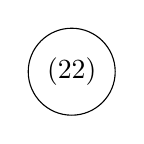
\begin{tikzpicture}[baseline=(n.base)]\node[draw,circle,inner sep=4pt] (n) {(22)};\end{tikzpicture}} * For a proper map of paracompact spaces, this condition just means that the fibers are ``aspheric'' namely ``contractible'' (in the Čech sense)}}}{\margin{\unsure{\diagram{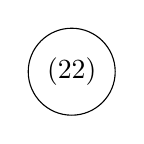
\begin{tikzpicture}[baseline=(n.base)]\node[draw,circle,inner sep=4pt] (n) {(22)};\end{tikzpicture}} * For a proper map of paracompact spaces, this condition just means that the fibers are ``aspheric'' namely ``contractible'' (in the Čech sense)}}}{marginal note placed}{ps_134-3_024-v0028}

%% END SOURCE ps_134-3_024
\ifnum\EditionMode=1
\psapparatusstart
\psentry{ps_134-3_024-v0001}{1}{typewriter deletion}{\xout{xx}}{}{The typewriter strikes out this material; it leaves the corrected running text.}
\psentry{ps_134-3_024-v0002}{2}{marginal note placed}{\margin{\diagram{\begin{tikzpicture}[x=1cm,y=1cm]\draw[->] (0.35,0)--(0,0)--(0,0.8);\end{tikzpicture}}}}{\margin{\diagram{\begin{tikzpicture}[x=1cm,y=1cm]\draw[->] (0.35,0)--(0,0)--(0,0.8);\end{tikzpicture}}}}{The marginal material is set at its source-line call; any internal cancellations and replacements are applied in the corrected form.}
\psentry{ps_134-3_024-v0003}{3}{typed insertion}{\inserted[typed]{many}}{many}{The typed insertion is incorporated at its indicated position; insertion brackets leave the running text.}
\psentry{ps_134-3_024-v0004}{4}{typewriter deletion}{\xout{that}}{}{The typewriter strikes out this material; it leaves the corrected running text.}
\psentry{ps_134-3_024-v0005}{5}{marginal note placed}{\margin{\diagram{\begin{tikzpicture}[x=1cm,y=1cm]\draw[->] (0.35,0.8)--(0,0.8)--(0,0);\end{tikzpicture}}}}{\margin{\diagram{\begin{tikzpicture}[x=1cm,y=1cm]\draw[->] (0.35,0.8)--(0,0.8)--(0,0);\end{tikzpicture}}}}{The marginal material is set at its source-line call; any internal cancellations and replacements are applied in the corrected form.}
\psentry{ps_134-3_024-v0006}{6}{writing over}{\over{\illegible{1}}{25}}{\hand{25}}{The superposed handwritten reading replaces the underlying reading.}
\psentry{ps_134-3_024-v0007}{7}{typewriter deletion}{\xout{which}}{}{The typewriter strikes out this material; it leaves the corrected running text.}
\psentry{ps_134-3_024-v0008}{8}{typewriter deletion}{\xout{if M is the}}{}{The typewriter strikes out this material; it leaves the corrected running text.}
\psentry{ps_134-3_024-v0009}{9}{typewriter deletion}{\xout{a}}{}{The typewriter strikes out this material; it leaves the corrected running text.}
\psentry{ps_134-3_024-v0010}{10}{deletion}{\deleted{page 19 ff}}{}{The author cancels this material by hand; it leaves the corrected running text.}
\psentry{ps_134-3_024-v0011}{11}{insertion}{\inserted{section 23}}{\hand{section 23}}{The handwritten insertion is incorporated at its indicated position; insertion brackets leave the running text.}
\psentry{ps_134-3_024-v0012}{12}{writing over}{\over{s}{r}}{\hand{r}}{The superposed handwritten reading replaces the underlying reading.}
\psentry{ps_134-3_024-v0013}{13}{deletion}{\deleted{inverse}}{}{The author cancels this material by hand; it leaves the corrected running text.}
\psentry{ps_134-3_024-v0014}{14}{insertion}{\inserted{direct}}{\hand{direct}}{The handwritten insertion is incorporated at its indicated position; insertion brackets leave the running text.}
\psentry{ps_134-3_024-v0015}{15}{typewriter deletion}{\xout{s}}{}{The typewriter strikes out this material; it leaves the corrected running text.}
\psentry{ps_134-3_024-v0016}{16}{deletion}{\deleted{'}}{}{The author cancels this material by hand; it leaves the corrected running text.}
\psentry{ps_134-3_024-v0017}{17}{marginal note placed}{\margin{\deleted{\illegible{1}}}}{\margin{}}{The marginal material is set at its source-line call; any internal cancellations and replacements are applied in the corrected form.}
\psentry{ps_134-3_024-v0018}{18}{marginal note placed}{\margin{\deleted{\illegible{1}}}}{\margin{}}{The marginal material is set at its source-line call; any internal cancellations and replacements are applied in the corrected form.}
\psentry{ps_134-3_024-v0019}{19}{deletion}{\deleted{\unsure{l}}}{}{The author cancels this material by hand; it leaves the corrected running text.}
\psentry{ps_134-3_024-v0020}{20}{typewriter deletion}{\xout{ acyclic}}{}{The typewriter strikes out this material; it leaves the corrected running text.}
\psentry{ps_134-3_024-v0021}{21}{typewriter deletion}{\xout{s}}{}{The typewriter strikes out this material; it leaves the corrected running text.}
\psentry{ps_134-3_024-v0022}{22}{insertion}{\inserted{arbitrary}}{\hand{arbitrary}}{The handwritten insertion is incorporated at its indicated position; insertion brackets leave the running text.}
\psentry{ps_134-3_024-v0023}{23}{typewriter deletion}{\xout{s}}{}{The typewriter strikes out this material; it leaves the corrected running text.}
\psentry{ps_134-3_024-v0024}{24}{insertion}{\inserted{sheaves}}{\hand{sheaves}}{The handwritten insertion is incorporated at its indicated position; insertion brackets leave the running text.}
\psentry{ps_134-3_024-v0025}{25}{typewriter deletion}{\xout{p}}{}{The typewriter strikes out this material; it leaves the corrected running text.}
\psentry{ps_134-3_024-v0026}{26}{typed insertion}{\inserted[typed]{Hot-}}{Hot-}{The typed insertion is incorporated at its indicated position; insertion brackets leave the running text.}
\psentry{ps_134-3_024-v0027}{27}{deletion}{\deleted{this}}{}{The author cancels this material by hand; it leaves the corrected running text.}
\psentry{ps_134-3_024-v0028}{28}{marginal note placed}{\margin{\unsure{\diagram{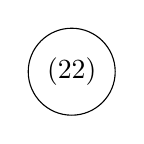
\begin{tikzpicture}[baseline=(n.base)]\node[draw,circle,inner sep=4pt] (n) {(22)};\end{tikzpicture}} * For a proper map of paracompact spaces, this condition just means that the fibers are ``aspheric'' namely ``contractible'' (in the Čech sense)}}}{\margin{\unsure{\diagram{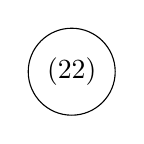
\begin{tikzpicture}[baseline=(n.base)]\node[draw,circle,inner sep=4pt] (n) {(22)};\end{tikzpicture}} * For a proper map of paracompact spaces, this condition just means that the fibers are ``aspheric'' namely ``contractible'' (in the Čech sense)}}}{The marginal material is set at its source-line call; any internal cancellations and replacements are applied in the corrected form.}
\psapparatusend
\fi
\pssource{ps_134-3_025}{134-3/25}{https://grothendieck.umontpellier.fr/web/viewer.html?file=../134-3.pdf\#page=26}
\psnumber{ps_134-3_025-v0001}{1}
\psnumber{ps_134-3_025-v0002}{2}
\psnumber{ps_134-3_025-v0003}{3}
\psnumber{ps_134-3_025-v0004}{4}
\psnumber{ps_134-3_025-v0005}{5}
\psnumber{ps_134-3_025-v0006}{6}
\psnumber{ps_134-3_025-v0007}{7}
\psnumber{ps_134-3_025-v0008}{8}
\psnumber{ps_134-3_025-v0009}{9}
\psnumber{ps_134-3_025-v0010}{10}
\psnumber{ps_134-3_025-v0011}{11}
\psnumber{ps_134-3_025-v0012}{12}
\psnumber{ps_134-3_025-v0013}{13}
\psnumber{ps_134-3_025-v0014}{14}
\psnumber{ps_134-3_025-v0015}{15}
\psnumber{ps_134-3_025-v0016}{16}
\psnumber{ps_134-3_025-v0017}{17}
%% BEGIN SOURCE ps_134-3_025
% Pursuing Stacks (cotes 134-2 to 134-8): archive cote 134-3, site page 25 (PDF page 26), typescript page 25.
% typescript. Draft compared: ps2.tex:1160-1224.
% AI-transcribed by Claude Opus 5.5 (claude-opus-5-5, adaptive thinking, effort high), Message Batches API, batch ps1 (msgbatch_01Rv5hCaNTtUt4JHx1yqoHPL), 2026-11-12; image review recorded in records/CHECK_DECISIONS_134_3_4.tsv.
\scanpage{134-3/25}
\var{\xout{25}}{}{typewriter deletion}{ps_134-3_025-v0001}
\mspage{25}

this class.  Maybe even it could be shown that this equivalence class
can be recovered in terms of the corresponding functor (*),  in the same
way as (according to Giraud) a ``topology'' on M can be recovered from
the associated subtopos of $M^{\hand{\wedge}}$\hand{,}namely the associated category of sheaves
on M (in such a way that the set of \var{\xout{subcategor}}{}{typewriter deletion}{ps_134-3_025-v0002}``topologies''on M can be
identified with the set of \var{\xout{\unsure{subt}}}{}{typewriter deletion}{ps_134-3_025-v0003}``closed subtopoi'' of $M^{\hand{\wedge}}$).  The very best
one could possibly hope for along these lines would be a one-to-one
correspondance between isomorphism classes of functors (*)(satisfying
certain properties ?),  and the so-called ``Hot-equivalence classes'' of
topologies on M.

Whether or not this tentative hope is excessive, when it comes to
the (still somewhat vague) question of understanding ``which algebraic
structure species are suitable for expressing homotopy types'',  it
might not be excessive though to expect that in all \var{\inserted[typed]{such}}{such}{typed insertion}{ps_134-3_025-v0004} cases,  M should
be equipped with just \uline{one} ``natural'' Hot-equivalence class of topologies
\var{\margin{\illegible{1}}}{\margin{\illegible{1}}}{marginal note placed}{ps_134-3_025-v0005}on M\var{\deleted{\illegible{1}}}{}{deletion}{ps_134-3_025-v0006}\hand{,}which moreover (one hopes,  or wonders) should be expressible
directly in terms of the \var{\inserted[typed]{intrinsic}}{intrinsic}{typed insertion}{ps_134-3_025-v0007} structure of M,  or,  what amounts to the same,
in terms of the \var{\inserted[typed]{full}}{full}{typed insertion}{ps_134-3_025-v0008} subcategory $\underline{B}$ of objects of ``finite presentation'',  \var{\xout{\unsure{givi}}}{}{typewriter deletion}{ps_134-3_025-v0009}
giving rise to M via the equivalence
\[ M \hand{\simeq} \mathrm{Ind}(\underline{B}) . \]
As we just saw in the case  M = (Cat),  the so-called ``canonical topolo-%
gy'' on M need not be within the natural Hot-equivalence class  -  and I
am at a loss for the moment to give a plausible intrinsic caracterizati-%
on of the latter,  in terms of the category M = (Cat). \hand{(${}^{22'}$).}

\var{\over{\unsure{25}}{26}}{\hand{26}}{writing over}{ps_134-3_025-v0010}.  What comes to mind though is that the categories such as \hand{$\Delta$} , \hand{$\square$}
and their analogons (corresponding to multicomplexes rather than mono-%
complexes, for instance\var{\over{\unsure{,}}{)}}{\hand{)}}{writing over}{ps_134-3_025-v0011}  can be viewed as (generally not full) subcate-%
gories of M  (in fact,  even of the smaller category (Ord) of all orde\unsure{\hand{red}}
sets).  The topologies we found on M were in fact associated in an evi-%
dent way to the choice of such subcategories.  As was already felt by
the end of the reflection two days ago (p.21),  these subcategories
(denoted there by $\underline{B}_{oo}$  ) have rather special features  -  they are
associated to \var{\inserted[typed]{simultaneous}}{simultaneous}{typed insertion}{ps_134-3_025-v0012} cellular decompositions of spheres of all dimensions  -
and it is this feature,  presumably,  that makes the associated ``trivial''
algebraic structure\var{\inserted{species}}{\hand{species}}{insertion}{ps_134-3_025-v0013}, giving rise to the category of set-theoretic
realizations  $\underline{B}_{oo}{}^{\hand{\wedge}}$ ,  eligible for ``describing homotopy types''.  In the
typical example M = (Cat) though,  contrarily to what was suggested \hand{by}
\var{\margin{\diagram{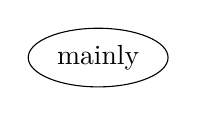
\begin{tikzpicture}[baseline=(n.base)]\node[draw,ellipse,inner sep=3pt] (n) {mainly};\end{tikzpicture}}}}{\margin{\diagram{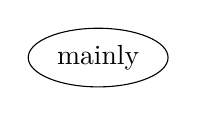
\begin{tikzpicture}[baseline=(n.base)]\node[draw,ellipse,inner sep=3pt] (n) {mainly};\end{tikzpicture}}}}{marginal note placed}{ps_134-3_025-v0014}\var{\deleted{on page 21}}{}{deletion}{ps_134-3_025-v0015} \var{\inserted{the end of section 23}}{\hand{the end of section 23}}{insertion}{ps_134-3_025-v0016} (when thinking \var{\inserted{mainly}}{\hand{mainly}}{insertion}{ps_134-3_025-v0017} of the rather special although important cases
when M is expressible  as a category  $B^{\hand{\wedge}}$\hand{,} for some category B such as

%% END SOURCE ps_134-3_025
\ifnum\EditionMode=1
\psapparatusstart
\psentry{ps_134-3_025-v0001}{1}{typewriter deletion}{\xout{25}}{}{The typewriter strikes out this material; it leaves the corrected running text.}
\psentry{ps_134-3_025-v0002}{2}{typewriter deletion}{\xout{subcategor}}{}{The typewriter strikes out this material; it leaves the corrected running text.}
\psentry{ps_134-3_025-v0003}{3}{typewriter deletion}{\xout{\unsure{subt}}}{}{The typewriter strikes out this material; it leaves the corrected running text.}
\psentry{ps_134-3_025-v0004}{4}{typed insertion}{\inserted[typed]{such}}{such}{The typed insertion is incorporated at its indicated position; insertion brackets leave the running text.}
\psentry{ps_134-3_025-v0005}{5}{marginal note placed}{\margin{\illegible{1}}}{\margin{\illegible{1}}}{The marginal material is set at its source-line call; any internal cancellations and replacements are applied in the corrected form.}
\psentry{ps_134-3_025-v0006}{6}{deletion}{\deleted{\illegible{1}}}{}{The author cancels this material by hand; it leaves the corrected running text.}
\psentry{ps_134-3_025-v0007}{7}{typed insertion}{\inserted[typed]{intrinsic}}{intrinsic}{The typed insertion is incorporated at its indicated position; insertion brackets leave the running text.}
\psentry{ps_134-3_025-v0008}{8}{typed insertion}{\inserted[typed]{full}}{full}{The typed insertion is incorporated at its indicated position; insertion brackets leave the running text.}
\psentry{ps_134-3_025-v0009}{9}{typewriter deletion}{\xout{\unsure{givi}}}{}{The typewriter strikes out this material; it leaves the corrected running text.}
\psentry{ps_134-3_025-v0010}{10}{writing over}{\over{\unsure{25}}{26}}{\hand{26}}{The superposed handwritten reading replaces the underlying reading.}
\psentry{ps_134-3_025-v0011}{11}{writing over}{\over{\unsure{,}}{)}}{\hand{)}}{The superposed handwritten reading replaces the underlying reading.}
\psentry{ps_134-3_025-v0012}{12}{typed insertion}{\inserted[typed]{simultaneous}}{simultaneous}{The typed insertion is incorporated at its indicated position; insertion brackets leave the running text.}
\psentry{ps_134-3_025-v0013}{13}{insertion}{\inserted{species}}{\hand{species}}{The handwritten insertion is incorporated at its indicated position; insertion brackets leave the running text.}
\psentry{ps_134-3_025-v0014}{14}{marginal note placed}{\margin{\diagram{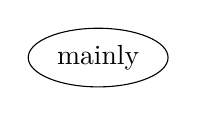
\begin{tikzpicture}[baseline=(n.base)]\node[draw,ellipse,inner sep=3pt] (n) {mainly};\end{tikzpicture}}}}{\margin{\diagram{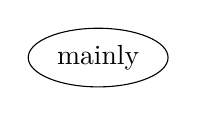
\begin{tikzpicture}[baseline=(n.base)]\node[draw,ellipse,inner sep=3pt] (n) {mainly};\end{tikzpicture}}}}{The marginal material is set at its source-line call; any internal cancellations and replacements are applied in the corrected form.}
\psentry{ps_134-3_025-v0015}{15}{deletion}{\deleted{on page 21}}{}{The author cancels this material by hand; it leaves the corrected running text.}
\psentry{ps_134-3_025-v0016}{16}{insertion}{\inserted{the end of section 23}}{\hand{the end of section 23}}{The handwritten insertion is incorporated at its indicated position; insertion brackets leave the running text.}
\psentry{ps_134-3_025-v0017}{17}{insertion}{\inserted{mainly}}{\hand{mainly}}{The handwritten insertion is incorporated at its indicated position; insertion brackets leave the running text.}
\psapparatusend
\fi
\pssource{ps_134-3_026}{134-3/26}{https://grothendieck.umontpellier.fr/web/viewer.html?file=../134-3.pdf\#page=27}
\psnumber{ps_134-3_026-v0001}{1}
\psnumber{ps_134-3_026-v0002}{2}
\psnumber{ps_134-3_026-v0003}{3}
\psnumber{ps_134-3_026-v0004}{4}
\psnumber{ps_134-3_026-v0005}{5}
%% BEGIN SOURCE ps_134-3_026
% Pursuing Stacks (cotes 134-2 to 134-8): archive cote 134-3, site page 26 (PDF page 27), typescript page 26.
% typescript. Draft compared: ps2.tex:1210-1267.
% AI-transcribed by Claude Opus 5.5 (claude-opus-5-5, adaptive thinking, effort high), Message Batches API, batch ps1 (msgbatch_01Rv5hCaNTtUt4JHx1yqoHPL), 2026-11-12; image review recorded in records/CHECK_DECISIONS_134_3_4.tsv.
\scanpage{134-3/26}
\mspage{26}

\hand{$\Delta$} ,\hand{$\square$} etc), there is no really privileged choice of such subcategory
$\underline{B}_{oo}$ - we found indeed a big bunch of such, the ones just as good as
the others. The point of course is that the corresponding topologies
on M, namely induced from the canonical topology on $\underline{B}_{oo}\hand{\hat{}}$ by the canoni-%
cal functor
\[ M \hand{\longrightarrow} \underline{B}_{oo}\hand{\hat{}} \quad , \]
are Hot-equivalent for some reason or other, which should be understood.
The plausible fact that emerges here, is that the ``natural'' Hot-equi-%
valence class of topologies on M is associated, in the way just descri-%
bed, to a \uline{class} (presumably an equivalence class in a suitable set for
suitable equivalence relation ...) \uline{of subcategories} $\underline{B}_{oo}$ \uline{in} M. The ques-%
tion of giving an intrinsic description of the former, is apparently
reduced to the (possibly more concrete) one, of giving an intrinsic
\unsure{descripttion|description} of a bunch of subcategories \var{\inserted[typed]{$B =$}}{$B =$}{typed insertion}{ps_134-3_026-v0001}$\underline{B}_{oo}$ of M. This description,
one feels, should both a) insist on intrinsic properties of B, inde-%
pendant of M namely of the structure species one is working with, and
b) be concerned with the particular way in which B is embedded in M,
which should by no means be an arbitrary one.

The properties a) should be, I guess, no more no less than those
which express that the ``trivial'' algebraic structure species defined by
B, giving a category of set-theoretic realizations $M_B = B\hand{\hat{}}$, should be
``suitable for describing homotopy types''. The examples at hand so
far suggest that in this case, the canonical topology on the topos $M_B$
is within the natural Hot-equivalence class, which gives a meaning to
the functor
\[ M_B = B\hand{\hat{}} \hand{\longrightarrow} (Hot) \quad , \]
indeed it associates to any a \hand{$\in$} Ob $\overset{\hand{\wedge}}{B}$ the homotopy type of the induced
\var{\margin{\deleted{because $\unsure{\widehat{B}_{/a} \simeq \widehat{B_{/a}}}$}}}{\margin{}}{marginal note placed}{ps_134-3_026-v0002}category $B_{/a}$ of all objects of B ``over a''\var{\inserted{(23)}}{\hand{(23)}}{insertion}{ps_134-3_026-v0003}. Thus a first condition on
B is that \uline{this functor should be a ``localization functor''}, identifying
(Hot) to a category of fractions of $M_B = B$\hand{$\hat{}$} . This does look indeed as
an\var{\inserted[typed]{extremely}}{extremely}{typed insertion}{ps_134-3_026-v0004}stringent dondition on B, and I wonder if the features we noticed in
the special cases dealt with so far, connected with cellular decomposi-%
tions of spheres, have any more compulsive significance than just
giving some handy \uline{sufficient} conditions (which deserve to be made expli-%
cit sooner or later \hand{!}) for ``eligibility'' of B for recovering (Hot). Be-%
yond this, one would \var{\inserted{of course}}{\hand{of course}}{insertion}{ps_134-3_026-v0005} like to have a better understanding of what it
\uline{really} means, in terms of the internal structure of B, that the
functor above from B\hand{$\hat{}$}\hand{/}to (Hot) is a localization functor.

%% END SOURCE ps_134-3_026
\ifnum\EditionMode=1
\psapparatusstart
\psentry{ps_134-3_026-v0001}{1}{typed insertion}{\inserted[typed]{$B =$}}{$B =$}{The typed insertion is incorporated at its indicated position; insertion brackets leave the running text.}
\psentry{ps_134-3_026-v0002}{2}{marginal note placed}{\margin{\deleted{because $\unsure{\widehat{B}_{/a} \simeq \widehat{B_{/a}}}$}}}{\margin{}}{The marginal material is set at its source-line call; any internal cancellations and replacements are applied in the corrected form.}
\psentry{ps_134-3_026-v0003}{3}{insertion}{\inserted{(23)}}{\hand{(23)}}{The handwritten insertion is incorporated at its indicated position; insertion brackets leave the running text.}
\psentry{ps_134-3_026-v0004}{4}{typed insertion}{\inserted[typed]{extremely}}{extremely}{The typed insertion is incorporated at its indicated position; insertion brackets leave the running text.}
\psentry{ps_134-3_026-v0005}{5}{insertion}{\inserted{of course}}{\hand{of course}}{The handwritten insertion is incorporated at its indicated position; insertion brackets leave the running text.}
\psapparatusend
\fi
\pssource{ps_134-3_027}{134-3/27}{https://grothendieck.umontpellier.fr/web/viewer.html?file=../134-3.pdf\#page=28}
\psnumber{ps_134-3_027-v0001}{1}
\psnumber{ps_134-3_027-v0002}{2}
\psnumber{ps_134-3_027-v0003}{3}
\psnumber{ps_134-3_027-v0004}{4}
\psnumber{ps_134-3_027-v0005}{5}
\psnumber{ps_134-3_027-v0006}{6}
\psnumber{ps_134-3_027-v0007}{7}
\psnumber{ps_134-3_027-v0008}{8}
\psnumber{ps_134-3_027-v0009}{9}
\psnumber{ps_134-3_027-v0010}{10}
\psnumber{ps_134-3_027-v0011}{11}
\psnumber{ps_134-3_027-v0012}{12}
\psnumber{ps_134-3_027-v0013}{13}
\psnumber{ps_134-3_027-v0014}{14}
\psnumber{ps_134-3_027-v0015}{15}
\psnumber{ps_134-3_027-v0016}{16}
\psnumber{ps_134-3_027-v0017}{17}
\psnumber{ps_134-3_027-v0018}{18}
\psnumber{ps_134-3_027-v0019}{19}
\psnumber{ps_134-3_027-v0020}{20}
\psnumber{ps_134-3_027-v0021}{21}
%% BEGIN SOURCE ps_134-3_027
% Pursuing Stacks (cotes 134-2 to 134-8): archive cote 134-3, site page 27 (PDF page 28), typescript page 27.
% typescript. Draft compared: ps2.tex:1256-1314.
% AI-transcribed by Claude Opus 5.5 (claude-opus-5-5, adaptive thinking, effort high), Message Batches API, batch ps1 (msgbatch_01Rv5hCaNTtUt4JHx1yqoHPL), 2026-11-12; image review recorded in records/CHECK_DECISIONS_134_3_4.tsv.
\scanpage{134-3/27}
\mspage{\hand{27}}

Once this internal condition on B is understood,  step b) then would
amount to describing,  in terms of an arbitrary ``eligible'' algebraic
structure species \var{\xout{xxxxx}}{}{typewriter deletion}{ps_134-3_027-v0001} expressed by the category M,  of what we should
mean by ``eligible functors'' \var{\xout{BxxxMxxx}}{}{typewriter deletion}{ps_134-3_027-v0002} \hand{$(^{29})$}\var{\margin{\unsure{we will rather say ``test functors'', see below\dots}}}{\margin{\unsure{we will rather say ``test functors'', see below\dots}}}{marginal note placed}{ps_134-3_027-v0003}
\[ B \hand{\longrightarrow} M \ , \]
giving rise in the usual way to a functor
\[ M \hand{\rightarrow} B^{\hand{\wedge}} \ . \]
In any case,  the latter functor defines upon M an induced \unsure{topology},
T say,  and the comparison \var{\inserted[typed]{lemma}}{lemma}{typed insertion}{ps_134-3_027-v0004} tells us that if either $B \hand{\rightarrow} M$ \var{\inserted[typed]{or $M \hand{\rightarrow} B^{\hand{\wedge}}$}}{or $M \hand{\rightarrow} B^{\hand{\wedge}}$}{typed insertion}{ps_134-3_027-v0005} is fully
faithful ,  then the topos associated to M is canonically equivalent\var{\xout{x}}{}{typewriter deletion}{ps_134-3_027-v0006}
to $B^{\hand{\wedge}}$  (using this comparison lemma for the functor which happens to be
fully faithful).  \var{\xout{Onxthexotherxhandx}}{}{typewriter deletion}{ps_134-3_027-v0007} From this follows that the functor
(*)  $M^{\hand{\sim}} \hand{\rightarrow}$ (Hot)  defined by T \var{\inserted{(cf. section 25)}}{\hand{(cf. section 25)}}{insertion}{ps_134-3_027-v0008} is nothing but the compositum
\[ M^{\hand{\sim}} \hand{\xrightarrow{\approx}} B^{\hand{\wedge}} \hand{\longrightarrow} (Hot) \quad , \]
and hence a localization functor.  In other words,  when B is a category
satisfying the condition seen above\hand{$(^{29})$}, then \uline{any} functor $B \hand{\rightarrow} M$ satisfying\var{\margin{\unsure{a ``test category'', as we will say}}}{\margin{\unsure{a ``test category'', as we will say}}}{marginal note placed}{ps_134-3_027-v0009}
one of the two fullness conditions above \var{\xout{xxx}}{}{typewriter deletion}{ps_134-3_027-v0010} yields a corresponding des-%
cription of (Hot) as a localization of $M^{\hand{\sim}}$.  What is still lacking though
is a grasp on when two such functors  $B \hand{\rightarrow} M$,  $B' \hand{\rightarrow} M$  define essentially
``the same'' functor  $M \hand{\rightarrow}$ (Hot),  or (more or less equivalently)  two
(Hot)-equivalent topologies T,T' on M;  \uline{is it enough,}  \uline{for instance,}
\uline{that they give rise to the same notion of} \uline{``weak equivalences''}  (namely\var{\margin{\unsure{same question arises for Hot-equivalence of topologies on M\dots}}}{\margin{\unsure{same question arises for Hot-equivalence of topologies on M\dots}}}{marginal note placed}{ps_134-3_027-v0011} \hand{\illegible{1}}
morphisms in M which are tranformed into an isomorphism of (Hot)) ?
And moreover,  \var{\xout{this}}{}{typewriter deletion}{ps_134-3_027-v0012} granting that this equivalence relation between
\var{\inserted[typed]{certain}}{certain}{typed insertion}{ps_134-3_027-v0013} full subcategories \var{\inserted{(say)}}{\hand{(say)}}{insertion}{ps_134-3_027-v0014} B of M is understood,  how define,in terms of M ,
a ``natural'' equivalence class of such full subcategories,  giving rise
to a \uline{canonical} functor  $M \hand{\rightarrow}$ (Hot) \var{\deleted{\hand{$(^{25})$}}}{}{deletion}{ps_134-3_027-v0015} \hand{?} \hand{$(^{25})$}

Recalling that the algebraic structure considered can be described
in terms of an arbitrary small category $\underline{B}$ where arbitrary finite direct
limits exist  (namely $\underline{B}$ is the full subcategory of M of objects of
finite presentation),  it seems reasonable to assume that indeed
\[ B \hand{\hookrightarrow} \underline{B} \quad \text{(a full embedding)} \ , \]
and the question transforms into describing a\var{\deleted{n}}{}{deletion}{ps_134-3_027-v0016} \var{\inserted[typed]{natural}}{natural}{typed insertion}{ps_134-3_027-v0017} equivalence class \var{\xout{xxxxx}}{}{typewriter deletion}{ps_134-3_027-v0018}
of such full subcategories,  in \var{\inserted[typed]{(more or less)}}{(more or less)}{typed insertion}{ps_134-3_027-v0019} any small category $\underline{B}$  where finite
direct limits exist,  and where moreover there exist such full subcate-%
gories B.  Also,  we may \var{\deleted{to}}{}{deletion}{ps_134-3_027-v0020} have to throw in some extra\var{\deleted{s}}{}{deletion}{ps_134-3_027-v0021} conditions on
$\underline{B}$ ,  such as the condition that direct sums be ``disjoint'' and ``universa\unsure{l}'' \hand{\unsure{$(^{*})$}}
already contemplated before.

%% END SOURCE ps_134-3_027
\ifnum\EditionMode=1
\psapparatusstart
\psentry{ps_134-3_027-v0001}{1}{typewriter deletion}{\xout{xxxxx}}{}{The typewriter strikes out this material; it leaves the corrected running text.}
\psentry{ps_134-3_027-v0002}{2}{typewriter deletion}{\xout{BxxxMxxx}}{}{The typewriter strikes out this material; it leaves the corrected running text.}
\psentry{ps_134-3_027-v0003}{3}{marginal note placed}{\margin{\unsure{we will rather say ``test functors'', see below\dots}}}{\margin{\unsure{we will rather say ``test functors'', see below\dots}}}{The marginal material is set at its source-line call; any internal cancellations and replacements are applied in the corrected form.}
\psentry{ps_134-3_027-v0004}{4}{typed insertion}{\inserted[typed]{lemma}}{lemma}{The typed insertion is incorporated at its indicated position; insertion brackets leave the running text.}
\psentry{ps_134-3_027-v0005}{5}{typed insertion}{\inserted[typed]{or $M \hand{\rightarrow} B^{\hand{\wedge}}$}}{or $M \hand{\rightarrow} B^{\hand{\wedge}}$}{The typed insertion is incorporated at its indicated position; insertion brackets leave the running text.}
\psentry{ps_134-3_027-v0006}{6}{typewriter deletion}{\xout{x}}{}{The typewriter strikes out this material; it leaves the corrected running text.}
\psentry{ps_134-3_027-v0007}{7}{typewriter deletion}{\xout{Onxthexotherxhandx}}{}{The typewriter strikes out this material; it leaves the corrected running text.}
\psentry{ps_134-3_027-v0008}{8}{insertion}{\inserted{(cf. section 25)}}{\hand{(cf. section 25)}}{The handwritten insertion is incorporated at its indicated position; insertion brackets leave the running text.}
\psentry{ps_134-3_027-v0009}{9}{marginal note placed}{\margin{\unsure{a ``test category'', as we will say}}}{\margin{\unsure{a ``test category'', as we will say}}}{The marginal material is set at its source-line call; any internal cancellations and replacements are applied in the corrected form.}
\psentry{ps_134-3_027-v0010}{10}{typewriter deletion}{\xout{xxx}}{}{The typewriter strikes out this material; it leaves the corrected running text.}
\psentry{ps_134-3_027-v0011}{11}{marginal note placed}{\margin{\unsure{same question arises for Hot-equivalence of topologies on M\dots}}}{\margin{\unsure{same question arises for Hot-equivalence of topologies on M\dots}}}{The marginal material is set at its source-line call; any internal cancellations and replacements are applied in the corrected form.}
\psentry{ps_134-3_027-v0012}{12}{typewriter deletion}{\xout{this}}{}{The typewriter strikes out this material; it leaves the corrected running text.}
\psentry{ps_134-3_027-v0013}{13}{typed insertion}{\inserted[typed]{certain}}{certain}{The typed insertion is incorporated at its indicated position; insertion brackets leave the running text.}
\psentry{ps_134-3_027-v0014}{14}{insertion}{\inserted{(say)}}{\hand{(say)}}{The handwritten insertion is incorporated at its indicated position; insertion brackets leave the running text.}
\psentry{ps_134-3_027-v0015}{15}{deletion}{\deleted{\hand{$(^{25})$}}}{}{The author cancels this material by hand; it leaves the corrected running text.}
\psentry{ps_134-3_027-v0016}{16}{deletion}{\deleted{n}}{}{The author cancels this material by hand; it leaves the corrected running text.}
\psentry{ps_134-3_027-v0017}{17}{typed insertion}{\inserted[typed]{natural}}{natural}{The typed insertion is incorporated at its indicated position; insertion brackets leave the running text.}
\psentry{ps_134-3_027-v0018}{18}{typewriter deletion}{\xout{xxxxx}}{}{The typewriter strikes out this material; it leaves the corrected running text.}
\psentry{ps_134-3_027-v0019}{19}{typed insertion}{\inserted[typed]{(more or less)}}{(more or less)}{The typed insertion is incorporated at its indicated position; insertion brackets leave the running text.}
\psentry{ps_134-3_027-v0020}{20}{deletion}{\deleted{to}}{}{The author cancels this material by hand; it leaves the corrected running text.}
\psentry{ps_134-3_027-v0021}{21}{deletion}{\deleted{s}}{}{The author cancels this material by hand; it leaves the corrected running text.}
\psapparatusend
\fi
\pssource{ps_134-3_028}{134-3/28}{https://grothendieck.umontpellier.fr/web/viewer.html?file=../134-3.pdf\#page=29}
\psnumber{ps_134-3_028-v0001}{1}
\psnumber{ps_134-3_028-v0002}{2}
\psnumber{ps_134-3_028-v0003}{3}
\psnumber{ps_134-3_028-v0004}{4}
\psnumber{ps_134-3_028-v0005}{5}
\psnumber{ps_134-3_028-v0006}{6}
\psnumber{ps_134-3_028-v0007}{7}
\psnumber{ps_134-3_028-v0008}{8}
%% BEGIN SOURCE ps_134-3_028
% Pursuing Stacks (cotes 134-2 to 134-8): archive cote 134-3, site page 28 (PDF page 29), typescript page 28.
% typescript. Draft compared: ps2.tex:1300-1362.
% AI-transcribed by Claude Opus 5.5 (claude-opus-5-5, adaptive thinking, effort high), Message Batches API, batch ps1 (msgbatch_01Rv5hCaNTtUt4JHx1yqoHPL), 2026-11-12; image review recorded in records/CHECK_DECISIONS_134_3_4.tsv.
\scanpage{134-3/28}
\mspage{\hand{28}}

Maybe I was a little overenthousiastic, when observing that for
any full embedding of a category B into M (let's call the categories B
giving rise to a localization functor $B^{\hand{\wedge}} \hand{\to} (\mathrm{Hot})$ \uline{homotopy-test} catego-%
ries\var{\deleted{x}}{}{deletion}{ps_134-3_028-v0001}, or simply \uline{test} categories) we get a localization functor
\[ M^{\hand{\sim}} = (M^{\hand{\unsure{\sim}}},T_B)^{\hand{\sim}} \hand{\to} (\mathrm{Hot}) \quad , \]
where $T_B$ is the topology on M corresponding to the full subcategory B.
After all, there is a long way in between M itself and the category of
sheaves $M^{\hand{\sim}}$ - and what we want is to get (Hot) as a localization of M
itself, not of $M^{\hand{\sim}}$. Tt is not even clear, without some extra assumpti-%
on, that the natural functor from M to $M^{\hand{\sim}}$ is fully faithful, namely
that M can be identified with a full subcategory of the category $M^{\hand{\sim}}$
we've got to localize to get (Hot). We definitely would like this to
be true, or what amounts to the same, that the functor $M \hand{\to} B^{\hand{\wedge}}$
defined by $B \hand{\to} M$ should be fully faithful ---which means also that
the full subcategory B of M is ``generating by strict epimorphisms''\hand{(26),}
namely that for every K in M , there exists a strictly epimorphic
family of morphisms $b_i \hand{\to} K$ , with sources $b_i$ in B. This interpretati-%
on of full faithfulness of $M \hand{\to} B^{\hand{\wedge}}$is OK when $B \hand{\to} M$ is fully faithful ,
a condition which I \var{\inserted{gradually}}{\hand{gradually}}{insertion}{ps_134-3_028-v0002} put into the fore without really compelling reason,
except that in those examples I have in mind and which are \uline{not} connected
with the theory of stacks of various kinds, this condition is satisfied
\var{\margin{$\lrcorner\!\ulcorner$}}{\margin{$\lrcorner\!\ulcorner$}}{marginal note placed}{ps_134-3_028-v0003}\uline{indeed.}\hand{$\rfloor\!\lceil$} Apparently, with this endless digression on algebraic models
for homotopy types, \var{\deleted{the}}{}{deletion}{ps_134-3_028-v0004} stacks (which I am supposed to be after, after
all) are kind of fading into the background ! Maybe we should after
all forget about fully faithfullness condition on either $B \hand{\to} M$ or
$M \hand{\to} B^{\hand{\wedge}}$, and just insist that the compositum
\[ M \hand{\to} M^{\hand{\sim}} \hand{\to} B^{\hand{\wedge}} \hand{\to} (\mathrm{Hot}) \]
(which can be described \var{\inserted[typed]{directly}}{directly}{typed insertion}{ps_134-3_028-v0005} in terms of the topology $T_B$ on M associated to
\var{\margin{(27)}}{\margin{(27)}}{marginal note placed}{ps_134-3_028-v0006}the functor $B \hand{\to} M$\hand{/}) should be a localization functor. I guess that for
a given M or $\underline{B}$ ,\hand{$\wedge$} the mere fact that there should exist a \hand{``}test category\hand{''}
B and a functor $B \hand{\to} M$, or $B \hand{\to} \underline{B}$ , having this property, is already a
very strong condition on the structure species considered, namely on
the category $\underline{B}$ whi\hand{?}ch embodies this structure. It \var{\xout{probably}}{}{typewriter deletion}{ps_134-3_028-v0007}\var{\inserted[typed]{possibly}}{possibly}{typed insertion}{ps_134-3_028-v0008} means that
the corresponding functor
\[ \underline{B} \hand{\to} (\mathrm{Hot}) \]
factors through a functor
\[ \underline{B} \hand{\to} (\mathrm{Hot})_{\mathrm{f.t.}} \qquad \text{(f.t. means ``finite type'')} \]
which is itself a localization functor. It is not wholly impossible,
after all, that this condition on a functor $B \hand{\to} \underline{B}$ (B a test category)
is so stringent, that all such functors (for variable B) must be

%% END SOURCE ps_134-3_028
\ifnum\EditionMode=1
\psapparatusstart
\psentry{ps_134-3_028-v0001}{1}{deletion}{\deleted{x}}{}{The author cancels this material by hand; it leaves the corrected running text.}
\psentry{ps_134-3_028-v0002}{2}{insertion}{\inserted{gradually}}{\hand{gradually}}{The handwritten insertion is incorporated at its indicated position; insertion brackets leave the running text.}
\psentry{ps_134-3_028-v0003}{3}{marginal note placed}{\margin{$\lrcorner\!\ulcorner$}}{\margin{$\lrcorner\!\ulcorner$}}{The marginal material is set at its source-line call; any internal cancellations and replacements are applied in the corrected form.}
\psentry{ps_134-3_028-v0004}{4}{deletion}{\deleted{the}}{}{The author cancels this material by hand; it leaves the corrected running text.}
\psentry{ps_134-3_028-v0005}{5}{typed insertion}{\inserted[typed]{directly}}{directly}{The typed insertion is incorporated at its indicated position; insertion brackets leave the running text.}
\psentry{ps_134-3_028-v0006}{6}{marginal note placed}{\margin{(27)}}{\margin{(27)}}{The marginal material is set at its source-line call; any internal cancellations and replacements are applied in the corrected form.}
\psentry{ps_134-3_028-v0007}{7}{typewriter deletion}{\xout{probably}}{}{The typewriter strikes out this material; it leaves the corrected running text.}
\psentry{ps_134-3_028-v0008}{8}{typed insertion}{\inserted[typed]{possibly}}{possibly}{The typed insertion is incorporated at its indicated position; insertion brackets leave the running text.}
\psapparatusend
\fi
\pssource{ps_134-3_029}{134-3/29}{https://grothendieck.umontpellier.fr/web/viewer.html?file=../134-3.pdf\#page=30}
\psnumber{ps_134-3_029-v0001}{1}
\psnumber{ps_134-3_029-v0002}{2}
\psnumber{ps_134-3_029-v0003}{3}
\psnumber{ps_134-3_029-v0004}{4}
\psnumber{ps_134-3_029-v0005}{5}
\psnumber{ps_134-3_029-v0006}{6}
\psnumber{ps_134-3_029-v0007}{7}
\psnumber{ps_134-3_029-v0008}{8}
\psnumber{ps_134-3_029-v0009}{9}
\psnumber{ps_134-3_029-v0010}{10}
\psnumber{ps_134-3_029-v0011}{11}
\psnumber{ps_134-3_029-v0012}{12}
\psnumber{ps_134-3_029-v0013}{13}
\psnumber{ps_134-3_029-v0014}{14}
\psnumber{ps_134-3_029-v0015}{15}
\psnumber{ps_134-3_029-v0016}{16}
\psnumber{ps_134-3_029-v0017}{17}
\psnumber{ps_134-3_029-v0018}{18}
\psnumber{ps_134-3_029-v0019}{19}
\psnumber{ps_134-3_029-v0020}{20}
\psnumber{ps_134-3_029-v0021}{21}
\psnumber{ps_134-3_029-v0022}{22}
%% BEGIN SOURCE ps_134-3_029
% Pursuing Stacks (cotes 134-2 to 134-8): archive cote 134-3, site page 29 (PDF page 30), typescript page 29.
% typescript. Draft compared: ps2.tex:1345-1417.
% AI-transcribed by Claude Opus 5.5 (claude-opus-5-5, adaptive thinking, effort high), Message Batches API, batch ps1 (msgbatch_01Rv5hCaNTtUt4JHx1yqoHPL), 2026-11-12; image review recorded in records/CHECK_DECISIONS_134_3_4.tsv.
\scanpage{134-3/29}
\mspage{\hand{29}}
already ``equivalent'', namely define Hot-equivalent topologies on $\underline{B}$ (or \var{\margin{\unsure{or|on}}}{\margin{\unsure{or|on}}}{marginal note placed}{ps_134-3_029-v0001}
$\underline{M}$ , equivalently), and hence define ``the same'' functor $M \hand{\to} (\mathrm{Hot})$ or
$\underline{B} \hand{\to} (\mathrm{Hot})_{\mathrm{f.t.}}$ .

\hand{2}\var{\over{\unsure{4}}{7}}{\hand{7}}{writing over}{ps_134-3_029-v0002}. \var{\xout{All this}}{}{typewriter deletion}{ps_134-3_029-v0003} All this is pretty much ``thin air conjecturing'' for the time being
- quite possibly the notion of a ``test category'' itself has to be con-%
siderably adjusted, namely \unsure{strenghhened|strengthened}, as well as the notion of \hand{a}
``test functor'' $B \hand{\to} \underline{B}$ or $B \hand{\to} M$ - \var{\deleted{that}}{}{deletion}{ps_134-3_029-v0004} some important features \var{\inserted{may}}{\hand{may}}{insertion}{ps_134-3_029-v0005} have
entirely escaped my attention. The one idea though which may prove per-%
haps a valid one, is that \var{\inserted[typed]{a}}{a}{typed insertion}{ps_134-3_029-v0006} suitable \var{\inserted[typed]{localization}}{localization}{typed insertion}{ps_134-3_029-v0007} functor\var{\xout{s}}{}{typewriter deletion}{ps_134-3_029-v0008}
(*) \qquad $M \hand{\to} (\mathrm{Hot})$
may be defined, using either various topologies on M (related by a
suitable ``Hot-equivalence'' relation), or various functors $B \hand{\to} M$ or
$B \hand{\to} \underline{B}$ of suitable ``test categories'' B, and how the two are related.
I do not wish to pursue much longer along these lines though, but
rather put \var{\inserted{now}}{\hand{now}}{insertion}{ps_134-3_029-v0009} into the picture a third way still for getting a functor
(*), namely through some more or less natural functor
(**) \qquad $M \hand{\to} (\mathrm{Spaces})$ \hand{,} \qquad $K \hand{\mapsto} \hand{|}K\hand{|}$ ,
called a ``geometric \var{\inserted[typed]{(or topologic)}}{(or topologic)}{typed insertion}{ps_134-3_029-v0010} realization functor''\hand{$^{(28)}$}. There \var{\xout{are}}{}{typewriter deletion}{ps_134-3_029-v0011}\var{\inserted[typed]{is a}}{is a}{typed insertion}{ps_134-3_029-v0012} pretty compelling
choice\var{\xout{s}}{}{typewriter deletion}{ps_134-3_029-v0013} for such a functor, in the case of (semisimplicial or cubical)
complexes or multicomplexes of various kinds, and accordingly for
the subcategories (Cat),(Preord),(Ord) of \var{\xout{(Cat}}{}{typewriter deletion}{ps_134-3_029-v0014} (Ss sets), using geome-%
tric realization of semisimplicial complexes. In the case of the consi-%
derably more sophisticated structure of Gr-stacks though (or the related
structure of stacks, which will be dealt with in much the same way
below), although there is a pretty natural choice for geometric
realization on the subcategory $\underline{B}_{\mathrm{oo}}$ \var{\xout{\illegible{1}}}{}{typewriter deletion}{ps_134-3_029-v0015} of M embodying the ``primitive\var{\xout{''}}{}{typewriter deletion}{ps_134-3_029-v0016}
structure'' (namely the structure of an $\mathrm{oo}$-graph, see below also)\var{\over{,}{;}}{\hand{;}}{writing over}{ps_134-3_029-v0017} it
has been seen that the extension of this to a functor on the whole of
M (via it's extension to the \var{\inserted[typed]{left}}{left}{typed insertion}{ps_134-3_029-v0018} coherator defining the structure species,
which we denoted by $\underline{B}$ at the beginning of these notes, but which is
not quite the $\underline{B}$ envisioned here) is by no means unique, that it depends
on a pretty big bunch of rather arbitrary choices. This indeterminacy
now appears as quite in keeping with the general aspect of a (still
somewhat hypothetical) theory of algebraic homotopy models, gradually
emerging from darkness. It parallels the corresponding indeterminacy
in the choice of an ``eligible'' topology on M (call these topologies
the \hand{``}\uline{test topologies}\hand{''}), or \var{\over{\illegible{1}}{of}}{\hand{of}}{writing over}{ps_134-3_029-v0019} \var{\xout{th}}{}{typewriter deletion}{ps_134-3_029-v0020} a test functor $B \hand{\to} M$. What I would
like now to do, before coming back to stacks, is to reflec\hand{t} a little
still about the relations \var{\deleted{of}}{}{deletion}{ps_134-3_029-v0021} \var{\inserted[typed]{between}}{between}{typed insertion}{ps_134-3_029-v0022} such choice of a ``geometric realization
functor'', and test topologies or test functors relative to M .

%% END SOURCE ps_134-3_029
\ifnum\EditionMode=1
\psapparatusstart
\psentry{ps_134-3_029-v0001}{1}{marginal note placed}{\margin{\unsure{or|on}}}{\margin{\unsure{or|on}}}{The marginal material is set at its source-line call; any internal cancellations and replacements are applied in the corrected form.}
\psentry{ps_134-3_029-v0002}{2}{writing over}{\over{\unsure{4}}{7}}{\hand{7}}{The superposed handwritten reading replaces the underlying reading.}
\psentry{ps_134-3_029-v0003}{3}{typewriter deletion}{\xout{All this}}{}{The typewriter strikes out this material; it leaves the corrected running text.}
\psentry{ps_134-3_029-v0004}{4}{deletion}{\deleted{that}}{}{The author cancels this material by hand; it leaves the corrected running text.}
\psentry{ps_134-3_029-v0005}{5}{insertion}{\inserted{may}}{\hand{may}}{The handwritten insertion is incorporated at its indicated position; insertion brackets leave the running text.}
\psentry{ps_134-3_029-v0006}{6}{typed insertion}{\inserted[typed]{a}}{a}{The typed insertion is incorporated at its indicated position; insertion brackets leave the running text.}
\psentry{ps_134-3_029-v0007}{7}{typed insertion}{\inserted[typed]{localization}}{localization}{The typed insertion is incorporated at its indicated position; insertion brackets leave the running text.}
\psentry{ps_134-3_029-v0008}{8}{typewriter deletion}{\xout{s}}{}{The typewriter strikes out this material; it leaves the corrected running text.}
\psentry{ps_134-3_029-v0009}{9}{insertion}{\inserted{now}}{\hand{now}}{The handwritten insertion is incorporated at its indicated position; insertion brackets leave the running text.}
\psentry{ps_134-3_029-v0010}{10}{typed insertion}{\inserted[typed]{(or topologic)}}{(or topologic)}{The typed insertion is incorporated at its indicated position; insertion brackets leave the running text.}
\psentry{ps_134-3_029-v0011}{11}{typewriter deletion}{\xout{are}}{}{The typewriter strikes out this material; it leaves the corrected running text.}
\psentry{ps_134-3_029-v0012}{12}{typed insertion}{\inserted[typed]{is a}}{is a}{The typed insertion is incorporated at its indicated position; insertion brackets leave the running text.}
\psentry{ps_134-3_029-v0013}{13}{typewriter deletion}{\xout{s}}{}{The typewriter strikes out this material; it leaves the corrected running text.}
\psentry{ps_134-3_029-v0014}{14}{typewriter deletion}{\xout{(Cat}}{}{The typewriter strikes out this material; it leaves the corrected running text.}
\psentry{ps_134-3_029-v0015}{15}{typewriter deletion}{\xout{\illegible{1}}}{}{The typewriter strikes out this material; it leaves the corrected running text.}
\psentry{ps_134-3_029-v0016}{16}{typewriter deletion}{\xout{''}}{}{The typewriter strikes out this material; it leaves the corrected running text.}
\psentry{ps_134-3_029-v0017}{17}{writing over}{\over{,}{;}}{\hand{;}}{The superposed handwritten reading replaces the underlying reading.}
\psentry{ps_134-3_029-v0018}{18}{typed insertion}{\inserted[typed]{left}}{left}{The typed insertion is incorporated at its indicated position; insertion brackets leave the running text.}
\psentry{ps_134-3_029-v0019}{19}{writing over}{\over{\illegible{1}}{of}}{\hand{of}}{The superposed handwritten reading replaces the underlying reading.}
\psentry{ps_134-3_029-v0020}{20}{typewriter deletion}{\xout{th}}{}{The typewriter strikes out this material; it leaves the corrected running text.}
\psentry{ps_134-3_029-v0021}{21}{deletion}{\deleted{of}}{}{The author cancels this material by hand; it leaves the corrected running text.}
\psentry{ps_134-3_029-v0022}{22}{typed insertion}{\inserted[typed]{between}}{between}{The typed insertion is incorporated at its indicated position; insertion brackets leave the running text.}
\psapparatusend
\fi
\pssource{ps_134-3_030}{134-3/30}{https://grothendieck.umontpellier.fr/web/viewer.html?file=../134-3.pdf\#page=31}
\psnumber{ps_134-3_030-v0001}{1}
\psnumber{ps_134-3_030-v0002}{2}
\psnumber{ps_134-3_030-v0003}{3}
\psnumber{ps_134-3_030-v0004}{4}
\psnumber{ps_134-3_030-v0005}{5}
\psnumber{ps_134-3_030-v0006}{6}
\psnumber{ps_134-3_030-v0007}{7}
\psnumber{ps_134-3_030-v0008}{8}
\psnumber{ps_134-3_030-v0009}{9}
\psnumber{ps_134-3_030-v0010}{10}
%% BEGIN SOURCE ps_134-3_030
% Pursuing Stacks (cotes 134-2 to 134-8): archive cote 134-3, site page 30 (PDF page 31), typescript page 30.
% typescript. Draft compared: ps2.tex:1400-1472.
% AI-transcribed by Claude Opus 5.5 (claude-opus-5-5, adaptive thinking, effort high), Message Batches API, batch ps1 (msgbatch_01Rv5hCaNTtUt4JHx1yqoHPL), 2026-11-12; image review recorded in records/CHECK_DECISIONS_134_3_4.tsv.
\scanpage{134-3/30}
\mspage{30}

8.3.

\var{\margin{28.}}{\margin{28.}}{marginal note placed}{ps_134-3_030-v0001} While writing down the notes yesterday\hand{,}and this morning still while
pondering a little more, there has been the ever increasing feeling that
I ``was burning'', namely turning around something very close, very simple-%
minded too surely, without quite getting hold of it yet. In such a situa-%
tion, it is next to impossible just to leave it at that and come to the
``ordre du jour'' (namely stacks) - and even the \var{\inserted[typed]{``little}}{``little}{typed insertion}{ps_134-3_030-v0002} reflection'' I was about
to write down last night (but it was really too late then to go on) will
have to wait I guess, about the ``geometric realization functors'', as I
feel it is getting me off rather, maybe just a little, from where it is
``burning'' !

There was one question f\var{\over{la}{la}}{\hand{la}}{writing over}{ps_134-3_030-v0003}rring up yesterday \var{\deleted{(p.27)}}{}{deletion}{ps_134-3_030-v0004}\var{\inserted{(section 26)}}{\hand{(section 26)}}{insertion}{ps_134-3_030-v0005} which I nearly
dismissed as kind of silly, namely whether two localization functors
\[ (*) \qquad M \hand{\to} (\mathrm{Hot}) \]
obtained in such and such a way were isomorphic (maybe even canonically
so ??) provided they defined the same notion of ``weak equivalences'', name-%
ly arrows transformed into isomorphisms by the localization functors. Now
this maybe isnt so silly after all, in view of the following
\uline{Assumption}: The category of equivalences of (Hot) with itself, and \var{\inserted{of}}{\hand{of}}{insertion}{ps_134-3_030-v0006} natu-%
ral isomorphisms (possibly even any morphisms) between such, is equivalent
to the one point category.

This means 1) any equivalence $(\mathrm{Hot})\hand{\xrightarrow{\approx}}(\mathrm{Hot})$ is isomorphic to the
identity functor, and 2) any automorphism of the identity functor (pos-%
sibly even any endomorphism ?) is the identity.

Maybe these are facts well-known to the experts, maybe not - it is
not my business here anyhow to set out to prove such kind of things. It
looks pretty plausible, because if there was any non trivial autoequiva -
lence of (Hot), or automorphism of its identity functor, I guess I would
have heard about it\hand{,} or something of the sort would flip to my mind. It
would not be so if we abelianized (Hot) some way or other, as there would
be the loop and suspension functors, and homotheties by -1\unsure{.} \var{\deleted{\hand{of $\mathrm{id}_{(\mathrm{Hot})}$}}}{}{deletion}{ps_134-3_030-v0007} \var{\inserted{as
automorphisms of the identity functor.}}{\hand{as
automorphisms of the identity functor.}}{insertion}{ps_134-3_030-v0008}

This assumption now can be rephrased, by stating that \uline{a localization}
\uline{functor} \var{\xout{(*)}}{}{typewriter deletion}{ps_134-3_030-v0009} (*) \uline{from any category M into} (Hot) \uline{is well determined}, \uline{up to}
\uline{a unique isomorphism}, \uline{when the corresponding class} $W \hand{\subset} \mathrm{F}\var{\over{l}{l}}{\hand{l}}{writing over}{ps_134-3_030-v0010}(M)$ \uline{of weak equi-}%
\uline{valences is known}, in positive response to yesterday's silly question!

Such situation (*) seems to me to merit a name. As the word ``model
category'' has already been used in a somewhat different and more sophisti-%
cated sense by Quillen, in the context of homotopy, I rather use another

%% END SOURCE ps_134-3_030
\ifnum\EditionMode=1
\psapparatusstart
\psentry{ps_134-3_030-v0001}{1}{marginal note placed}{\margin{28.}}{\margin{28.}}{The marginal material is set at its source-line call; any internal cancellations and replacements are applied in the corrected form.}
\psentry{ps_134-3_030-v0002}{2}{typed insertion}{\inserted[typed]{``little}}{``little}{The typed insertion is incorporated at its indicated position; insertion brackets leave the running text.}
\psentry{ps_134-3_030-v0003}{3}{writing over}{\over{la}{la}}{\hand{la}}{The superposed handwritten reading replaces the underlying reading.}
\psentry{ps_134-3_030-v0004}{4}{deletion}{\deleted{(p.27)}}{}{The author cancels this material by hand; it leaves the corrected running text.}
\psentry{ps_134-3_030-v0005}{5}{insertion}{\inserted{(section 26)}}{\hand{(section 26)}}{The handwritten insertion is incorporated at its indicated position; insertion brackets leave the running text.}
\psentry{ps_134-3_030-v0006}{6}{insertion}{\inserted{of}}{\hand{of}}{The handwritten insertion is incorporated at its indicated position; insertion brackets leave the running text.}
\psentry{ps_134-3_030-v0007}{7}{deletion}{\deleted{\hand{of $\mathrm{id}_{(\mathrm{Hot})}$}}}{}{The author cancels this material by hand; it leaves the corrected running text.}
\psentry{ps_134-3_030-v0008}{8}{insertion}{\inserted{as
automorphisms of the identity functor.}}{\hand{as
automorphisms of the identity functor.}}{The handwritten insertion is incorporated at its indicated position; insertion brackets leave the running text.}
\psentry{ps_134-3_030-v0009}{9}{typewriter deletion}{\xout{(*)}}{}{The typewriter strikes out this material; it leaves the corrected running text.}
\psentry{ps_134-3_030-v0010}{10}{writing over}{$\over{l}{l}$}{$\hand{l}$}{The superposed handwritten reading replaces the underlying reading.}
\psapparatusend
\fi
\pssource{ps_134-3_031}{134-3/31}{https://grothendieck.umontpellier.fr/web/viewer.html?file=../134-3.pdf\#page=32}
\psnumber{ps_134-3_031-v0001}{1}
\psnumber{ps_134-3_031-v0002}{2}
\psnumber{ps_134-3_031-v0003}{3}
\psnumber{ps_134-3_031-v0004}{4}
\psnumber{ps_134-3_031-v0005}{5}
\psnumber{ps_134-3_031-v0006}{6}
\psnumber{ps_134-3_031-v0007}{7}
%% BEGIN SOURCE ps_134-3_031
% Pursuing Stacks (cotes 134-2 to 134-8): archive cote 134-3, site page 31 (PDF page 32), typescript page 31.
% typescript. Draft compared: ps2.tex:1456-1532.
% AI-transcribed by Claude Opus 5.5 (claude-opus-5-5, adaptive thinking, effort high), Message Batches API, batch ps1 (msgbatch_01Rv5hCaNTtUt4JHx1yqoHPL), 2026-11-12; image review recorded in records/CHECK_DECISIONS_134_3_4.tsv.
\scanpage{134-3/31}
\mspage{31}
one in the situation here. Let's call a ``modelizing category'', or sinply
a ``\uline{modelizer}'' ( ``modélisatrice'' in French), any category $M$, endowed with
a set $W\hand{\subset} \mathrm{Fl}(M)$ (the weak equivalences), satisfying the obvious condition:

(M\unsure{\hand{o}}d) a) $W$ is the set of arrows made invertible by the localization
functor $M\hand{\to} W^{-1}M$ \hand{(28')}, and
b) $W^{-1}M$ is equivalent to (Hot) ,
or equivalently, there exists a localization functor (*) (necessarily
unique up to unique isomorphism) such that $W$ be the set of arrows made
invertible by this functor.

Let $(M,W)$, $(M',W')$ be two modelizers, a functor \var{\inserted[typed]{$F$:}}{$F$:}{typed insertion}{ps_134-3_031-v0001} $M\hand{\to} M'$ is called
\uline{model-preserving}, or a \uline{morphism} between the modelizers, if it satisfies
either of the two following equivalent conditions:
(i) $F(W)\hand{\subset} W'$\hand{,} hence a functor $F_{W,W'} : W^{-1}M\hand{\to} W'^{-1}M'$, and the latter
is an equivalence.
(ii) The diagram
% Hand-drawn arrows are marked blue; typed objects remain plain.
\diagram{\begin{tikzcd}[column sep=small]
M \arrow[color=blue, rr, "F"] \arrow[color=blue, dr] \& \& M' \arrow[color=blue, dl] \\
\& \text{(Hot)} \&
\end{tikzcd}}
is commutative up to isomorphism (where the vertical arrows
are the \var{\xout{``model}}{}{typewriter deletion}{ps_134-3_031-v0002} ``type functors'' associated to $M$, $M'$ respectively\hand{)}

When dealing with a modelizer $(M,W)$, $W$ will be generally understood
so that we write simply \hand{$M$}. When $M$ is defined in terms of an algebraic
structure species, the task arises to find out whether (if any) there
exists a \uline{unique} $W\hand{\subset} \mathrm{Fl}(M)$ turning $M$ into a modelizer, and if not so, if
we can however pinpoint one which is a more natural one, and which we
would call ``canonical''.

Here is a diagram including most of the modelizers and model-preserving
functors between these which we met so far\hand{,}\hand{(29)} \var{\deleted{\xout{with the}}}{}{deletion}{ps_134-3_031-v0003} \hand{(}not included however
those connected with the theory of ``higher'' stacks and Gr-stacks, wh ich we
will have to elaborate upon later on\hand{)}:
\var{\margin{\diagram{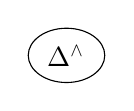
\begin{tikzpicture}[baseline=(n.base)]\node[draw,ellipse,inner sep=3pt] (n) {$\Delta^\wedge$};\end{tikzpicture}}}}{\margin{\diagram{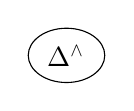
\begin{tikzpicture}[baseline=(n.base)]\node[draw,ellipse,inner sep=3pt] (n) {$\Delta^\wedge$};\end{tikzpicture}}}}{marginal note placed}{ps_134-3_031-v0004}
\var{\margin{\diagram{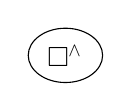
\begin{tikzpicture}[baseline=(n.base)]\node[draw,ellipse,inner sep=3pt] (n) {$\square^\wedge$};\end{tikzpicture}}}}{\margin{\diagram{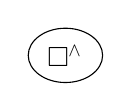
\begin{tikzpicture}[baseline=(n.base)]\node[draw,ellipse,inner sep=3pt] (n) {$\square^\wedge$};\end{tikzpicture}}}}{marginal note placed}{ps_134-3_031-v0005}
% Hand-drawn arrows are marked blue; typed objects remain plain.
\diagram{\begin{tikzcd}[row sep=small, column sep=small]
\& \& \& \hand{\hat{\Delta}}=\text{(ss. sets)} \arrow[color=blue, dr, "\hand{\xi}"] \& \\
\text{(Ord)} \arrow[color=blue, r, hook] \& \text{(Preord)} \arrow[color=blue, r, hook] \& \text{(Cat)} \arrow[color=blue, ur, "\hand{\alpha}"] \arrow[color=blue, dr, "\hand{\beta}"'] \& \& \text{(Cat)} \\
\& \& \& \hand{\square}=\text{(cub. sets)} \arrow[color=blue, ur, "\hand{\eta}"'] \&
\end{tikzcd}}
where the two last functors, with values in (Cat), are the two obvious
functors, obtained from
\hand{(**)} \hand{$i_A$}: $A^{\hand{\wedge}}\hand{\to}$ (Cat) , \var{\over{a}{$F$}}{\hand{$F$}}{writing over}{ps_134-3_031-v0006} $\hand{\mapsto} A_{/\var{\over{a}{F}}{\hand{F}}{writing over}{ps_134-3_031-v0007}}$
by particularizing to $A=$\hand{$\Delta$} or \hand{$\square$}. As we noticed before, the four first
among these six functors admit left adjoints, but except for the first,
these adjoints are \uline{not} model preserving. The two last functors, and more

%% END SOURCE ps_134-3_031
\ifnum\EditionMode=1
\psapparatusstart
\psentry{ps_134-3_031-v0001}{1}{typed insertion}{\inserted[typed]{$F$:}}{$F$:}{The typed insertion is incorporated at its indicated position; insertion brackets leave the running text.}
\psentry{ps_134-3_031-v0002}{2}{typewriter deletion}{\xout{``model}}{}{The typewriter strikes out this material; it leaves the corrected running text.}
\psentry{ps_134-3_031-v0003}{3}{deletion}{\deleted{\xout{with the}}}{}{The author cancels this material by hand; it leaves the corrected running text.}
\psentry{ps_134-3_031-v0004}{4}{marginal note placed}{\margin{\diagram{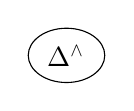
\begin{tikzpicture}[baseline=(n.base)]\node[draw,ellipse,inner sep=3pt] (n) {$\Delta^\wedge$};\end{tikzpicture}}}}{\margin{\diagram{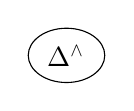
\begin{tikzpicture}[baseline=(n.base)]\node[draw,ellipse,inner sep=3pt] (n) {$\Delta^\wedge$};\end{tikzpicture}}}}{The marginal material is set at its source-line call; any internal cancellations and replacements are applied in the corrected form.}
\psentry{ps_134-3_031-v0005}{5}{marginal note placed}{\margin{\diagram{\begin{tikzpicture}[baseline=(n.base)]\node[draw,ellipse,inner sep=3pt] (n) {$\square^\wedge$};\end{tikzpicture}}}}{\margin{\diagram{\begin{tikzpicture}[baseline=(n.base)]\node[draw,ellipse,inner sep=3pt] (n) {$\square^\wedge$};\end{tikzpicture}}}}{The marginal material is set at its source-line call; any internal cancellations and replacements are applied in the corrected form.}
\psentry{ps_134-3_031-v0006}{6}{writing over}{\over{a}{$F$}}{\hand{$F$}}{The superposed handwritten reading replaces the underlying reading.}
\psentry{ps_134-3_031-v0007}{7}{writing over}{$\over{a}{F}$}{$\hand{F}$}{The superposed handwritten reading replaces the underlying reading.}
\psapparatusend
\fi
\pssource{ps_134-3_032}{134-3/32}{https://grothendieck.umontpellier.fr/web/viewer.html?file=../134-3.pdf\#page=33}
\psnumber{ps_134-3_032-v0001}{1}
\psnumber{ps_134-3_032-v0002}{2}
\psnumber{ps_134-3_032-v0003}{3}
\psnumber{ps_134-3_032-v0004}{4}
\psnumber{ps_134-3_032-v0005}{5}
\psnumber{ps_134-3_032-v0006}{6}
\psnumber{ps_134-3_032-v0007}{7}
\psnumber{ps_134-3_032-v0008}{8}
\psnumber{ps_134-3_032-v0009}{9}
\psnumber{ps_134-3_032-v0010}{10}
\psnumber{ps_134-3_032-v0011}{11}
\psnumber{ps_134-3_032-v0012}{12}
%% BEGIN SOURCE ps_134-3_032
% Pursuing Stacks (cotes 134-2 to 134-8): archive cote 134-3, site page 32 (PDF page 33), typescript page 32.
% typescript. Draft compared: ps2.tex:1514-1585.
% AI-transcribed by Claude Opus 5.5 (claude-opus-5-5, adaptive thinking, effort high), Message Batches API, batch ps1 (msgbatch_01Rv5hCaNTtUt4JHx1yqoHPL), 2026-11-12; image review recorded in records/CHECK_DECISIONS_134_3_4.tsv.
\scanpage{134-3/32}
\mspage{32}

generally the functor (**), admit right adjoints, namely the functor

\var{\xout{(Cat)xxxx$\hat{A}$xxxxxxaxxxxHomx}}{}{typewriter deletion}{ps_134-3_032-v0001}

$j_A$: \quad (Cat) $\hand{\longrightarrow} A^{\hand{\wedge}}$ \quad , \quad where \quad $j_A(B) = (\ a \hand{\mapsto} \mathrm{Hom}(A_{/a},B))$ \quad (B $\hand{\in}$ Ob(Cat)
% NOTE: the right edge of the page cuts the end of this line; a handwritten mark (bracket?) stands there
It should be noted that the functors \quad $j_{\hand{\Delta}}$ , $j_{\hand{\square}}$ are \uline{not} the two functors \hand{$\alpha,\beta$}
% Hand-drawn arrows are marked blue; typed objects remain plain.
\diagram{\begin{tikzcd}[row sep=tiny] \& \hand{\Delta}^{\hand{\wedge}} \\ \text{(Cat)} \ar[color=blue, ur] \ar[color=blue, dr] \& \\ \& \hand{\square}^{\hand{\wedge}} \end{tikzcd}} which appear in the diagram above, \quad the latter are associated
to the familiar functors

% Hand-drawn arrows are marked blue; typed objects remain plain.
\var{\margin{(***)}}{\margin{(***)}}{marginal note placed}{ps_134-3_032-v0002} \diagram{\begin{tikzcd}[row sep=tiny] \hand{\Delta} \ar[color=blue, dr] \& \\ \& \text{(Cat)} \\ \hand{\square} \ar[color=blue, ur] \& \end{tikzcd}}

(factoring in fact through (Ord)), associating to every ordered simplex,
or to every multioriented cube, \quad the corresponding 1-skeleton with suitable
orientations on the edges, turning \var{\inserted[typed]{the vertices of}}{the vertices of}{typed insertion}{ps_134-3_032-v0003} this graph into an ordered set; \quad while
the two former are associated to the functors deduced from (**) by restric-%
ting to $A \hand{\subset} A^{\hand{\wedge}}$ , \quad namely
\[ n \hand{\mapsto} \hand{\Delta}\hand{/}\hand{\Delta}_n \]
in the case of \hand{$\Delta$}, \quad and accordingly for \hand{$\square$}. \quad The values of these functors,
contrarily to the two preceding ones, \quad are \uline{infinite} categories, \quad and they
cannot be described by \var{\inserted{(i.e. ``are'' not)}}{\hand{(i.e. ``are'' not)}}{insertion}{ps_134-3_032-v0004} (pre)ordered sets. \quad If however we had defined
the categories \hand{$\Delta$} , \hand{$\square$} \quad in terms of iterated boundary operations only, \quad exclu%
% NOTE: the right edge of the page cuts the end of the line after "exclu"
ding the degeneracy operations (which, \quad I feel, \quad are not really needed for
turning \hand{$\Delta^\wedge$} and \hand{$\square^\wedge$} into model\var{\over{ato}{ize}}{\hand{ize}}{writing over}{ps_134-3_032-v0005}rs), \quad we would get indeed \uline{finite} ordered
sets, \quad namely the full combinatorial simplices or cubes, \var{\inserted[typed]{each one}}{each one}{typed insertion}{ps_134-3_032-v0006} embodied by the
ordered set of all it's facettes of all possible dimensions.

Contrarily to what happens with the functors \hand{$\alpha$, $\beta$}, \quad I feel that for
the two functors \hand{$\xi,\eta$} in opposite direction, \quad not only are they model pre-%
serving, \quad but the \var{\inserted[typed]{right}}{right}{typed insertion}{ps_134-3_032-v0007} adjoint functors \quad $j_{\hand{\Delta}}$ , $j_{\hand{\square}}$ must be model preserving too,
and we will have to come back upon this in a more general context.

We could amplify and unify somewhat the previous diagram of modelizers,
by introducing multicomplexes, \quad which after all can be as well ``mixed''
namely partly semisimplicial, \quad partly cubical. \quad Namely, \quad we may introduce
the would-be \var{\inserted{``}}{\hand{``}}{insertion}{ps_134-3_032-v0008}test categories'' \hand{(30)}
\[ (\hand{\Delta})^p \hand{\times} (\hand{\Delta})^q = T_{p,q} \qquad (p,q \hand{\in} \underline{N} \ , \quad p+q \var{\over{>}{\geq}}{\hand{\geq}}{writing over}{ps_134-3_032-v0009} 1) \]
giving rise to the category \quad $T^{\hand{\wedge}}_{p,q}$ \var{\deleted{\unsure{x}}}{}{deletion}{ps_134-3_032-v0010} \quad of (p,q)-multicomplexes (p times
simplicial, q times cubical). \quad \var{\xout{The}}{}{typewriter deletion}{ps_134-3_032-v0011} We have a natural functor (generalizing
the functors (xxx))
\[ T_{p,q} \hand{\longrightarrow} \text{(Ord)} \hand{(} \hand{\hookrightarrow} \text{(Cat)} \hand{)} \ , \]
associating to a system of p standart simplices and q standart cubes
(of variable dimensions), \quad the \uline{product} of the p+q associated ordered sets.
We get this way a functor
\[ \hand{\alpha_{p,q}} \ \var{\deleted{\hand{\illegible{1}_{p,q}}}}{}{deletion}{ps_134-3_032-v0012} : \text{(Cat)} \hand{\longrightarrow} T^{\hand{\wedge}}_{p,q} \]

%% END SOURCE ps_134-3_032
\ifnum\EditionMode=1
\psapparatusstart
\psentry{ps_134-3_032-v0001}{1}{typewriter deletion}{\xout{(Cat)xxxx$\hat{A}$xxxxxxaxxxxHomx}}{}{The typewriter strikes out this material; it leaves the corrected running text.}
\psentry{ps_134-3_032-v0002}{2}{marginal note placed}{\margin{(***)}}{\margin{(***)}}{The marginal material is set at its source-line call; any internal cancellations and replacements are applied in the corrected form.}
\psentry{ps_134-3_032-v0003}{3}{typed insertion}{\inserted[typed]{the vertices of}}{the vertices of}{The typed insertion is incorporated at its indicated position; insertion brackets leave the running text.}
\psentry{ps_134-3_032-v0004}{4}{insertion}{\inserted{(i.e. ``are'' not)}}{\hand{(i.e. ``are'' not)}}{The handwritten insertion is incorporated at its indicated position; insertion brackets leave the running text.}
\psentry{ps_134-3_032-v0005}{5}{writing over}{\over{ato}{ize}}{\hand{ize}}{The superposed handwritten reading replaces the underlying reading.}
\psentry{ps_134-3_032-v0006}{6}{typed insertion}{\inserted[typed]{each one}}{each one}{The typed insertion is incorporated at its indicated position; insertion brackets leave the running text.}
\psentry{ps_134-3_032-v0007}{7}{typed insertion}{\inserted[typed]{right}}{right}{The typed insertion is incorporated at its indicated position; insertion brackets leave the running text.}
\psentry{ps_134-3_032-v0008}{8}{insertion}{\inserted{``}}{\hand{``}}{The handwritten insertion is incorporated at its indicated position; insertion brackets leave the running text.}
\psentry{ps_134-3_032-v0009}{9}{writing over}{$\over{>}{\geq}$}{$\hand{\geq}$}{The superposed handwritten reading replaces the underlying reading.}
\psentry{ps_134-3_032-v0010}{10}{deletion}{\deleted{\unsure{x}}}{}{The author cancels this material by hand; it leaves the corrected running text.}
\psentry{ps_134-3_032-v0011}{11}{typewriter deletion}{\xout{The}}{}{The typewriter strikes out this material; it leaves the corrected running text.}
\psentry{ps_134-3_032-v0012}{12}{deletion}{$\deleted{\hand{\illegible{1}_{p,q}}}$}{}{The author cancels this material by hand; it leaves the corrected running text.}
\psapparatusend
\fi
\pssource{ps_134-3_033}{134-3/33}{https://grothendieck.umontpellier.fr/web/viewer.html?file=../134-3.pdf\#page=34}
\psnumber{ps_134-3_033-v0001}{1}
\psnumber{ps_134-3_033-v0002}{2}
\psnumber{ps_134-3_033-v0003}{3}
\psnumber{ps_134-3_033-v0004}{4}
\psnumber{ps_134-3_033-v0005}{5}
\psnumber{ps_134-3_033-v0006}{6}
\psnumber{ps_134-3_033-v0007}{7}
\psnumber{ps_134-3_033-v0008}{8}
\psnumber{ps_134-3_033-v0009}{9}
\psnumber{ps_134-3_033-v0010}{10}
\psnumber{ps_134-3_033-v0011}{11}
\psnumber{ps_134-3_033-v0012}{12}
%% BEGIN SOURCE ps_134-3_033
% Pursuing Stacks (cotes 134-2 to 134-8): archive cote 134-3, site page 33 (PDF page 34), typescript page 33.
% typescript. Draft compared: ps2.tex:1567-1638.
% AI-transcribed by Claude Opus 5.5 (claude-opus-5-5, adaptive thinking, effort high), Message Batches API, batch ps1 (msgbatch_01Rv5hCaNTtUt4JHx1yqoHPL), 2026-11-12; image review recorded in records/CHECK_DECISIONS_134_3_4.tsv.
\scanpage{134-3/33}
\mspage{\hand{33}}
which presumably (as I already felt yesterday, cf first lines p.24) is not
any less model-preserving than the functors $\hand{\alpha},\hand{\beta}$ it generalizes.  Of course,
taking A = $T_{p,q}$ above,  we equally get a natural functor
\[ \hand{i_{p,q}} : T^{\hand{\wedge}}_{p,q} \hand{\longrightarrow} (\mathrm{Cat}) \]
\var{\margin{\diagram{\begin{tikzpicture}[x=1em,y=1em]\draw[->] (1.7,0)--(.2,0) .. controls (0,0) and (0,.2) .. (0,.5)--(0,2.1);\end{tikzpicture}}}}{\margin{\diagram{\begin{tikzpicture}[x=1em,y=1em]\draw[->] (1.7,0)--(.2,0) .. controls (0,0) and (0,.2) .. (0,.5)--(0,2.1);\end{tikzpicture}}}}{marginal note placed}{ps_134-3_033-v0001} admitting a right adjoint\var{\inserted{$j_{p,q}$}}{\hand{$j_{p,q}$}}{insertion}{ps_134-3_033-v0002}, and both functors I feel must be model preser-%
ving.

\var{\over{\unsure{26}}{29}}{\hand{29}}{writing over}{ps_134-3_033-v0003}.  It is time now to elaborate a little upon the notion of a test catego-%
ry,  within the context of modelizers.  Let A be a small category,  and
consider  the functor (**)
\var{\margin{\diagram{\begin{tikzpicture}[x=1em,y=1em]\draw[->] (1.7,0)--(.2,0) .. controls (0,0) and (0,-.2) .. (0,-.5)--(0,-2.8);\end{tikzpicture}}}}{\margin{\diagram{\begin{tikzpicture}[x=1em,y=1em]\draw[->] (1.7,0)--(.2,0) .. controls (0,0) and (0,-.2) .. (0,-.5)--(0,-2.8);\end{tikzpicture}}}}{marginal note placed}{ps_134-3_033-v0004} (**) \[ \hand{i}_{A} : A^{\hand{\wedge}} \hand{\longrightarrow} (\mathrm{Cat}) \quad , \quad F \hand{\mapsto} A_{/F} \quad , \]
Whenever we have a functor \var{\inserted[typed]{i:}}{i:}{typed insertion}{ps_134-3_033-v0005} $M \hand{\to} M'$,  when $M'$ is equipped with a $W'$ turning
it into a modelizer,  there is (if any) \var{\xout{xx}}{}{typewriter deletion}{ps_134-3_033-v0006} just one $W \hand{\subset} \mathrm{F}\var{\over{l}{l}}{\hand{l}}{writing over}{ps_134-3_033-v0007}(M)$ turning M into
a modelizer and i into a morphism of such,  namely $W = i_{\mathrm{F}\var{\over{l}{l}}{\hand{l}}{writing over}{ps_134-3_033-v0008}}^{-1}(W')$.  In any
case,  we may define W (``weak equivalences'') by this formula,  and get a
functor
\[ W^{-1}M \hand{\longrightarrow} W'^{-1}M' \quad , \]
which is an equivalence iff (M,W) is indeed a modelizer and i model\var{\xout{\unsure{s}}}{}{typewriter deletion}{ps_134-3_033-v0009}preser-%
ving.  We may say shortly that i: $M \hand{\to} M'$ is model preserving,  even without
any W given beforehand.  Now coming back to the situation  (**),  the under-%
standing yesterday was to call A a \uline{test} \uline{category} ,  to express that the
canonical functor (**) is model preserving. \hand{(}In any case,  unless otherwise
specified by the context, we will refer to arrows in $A\hand{^{\wedge}}$ which are transfor-%
med into weak equivalences of (Cat)  as ``\uline{weak equivalences}''.\hand{)} It may well
turn out,  by the way,  that we will have to restrict somewhat still the
notion of a test category.

\var{\margin{\diagram{\begin{tikzpicture}[x=1em,y=1em]\draw (0,0)--(0,-3.7);\draw (.17,0)--(.17,-3.7);\end{tikzpicture}}}}{\margin{\diagram{\begin{tikzpicture}[x=1em,y=1em]\draw (0,0)--(0,-3.7);\draw (.17,0)--(.17,-3.7);\end{tikzpicture}}}}{marginal note placed}{ps_134-3_033-v0010} In any case,  \uline{the basic modelizer,}  \uline{in this whole approach to homotopy}
\uline{models,}  \uline{is by no means the category} (Ss sets)  (however handy)  \uline{or the}
\uline{category} (Spaces)  (howeve\var{\xout{\unsure{t}}}{}{typewriter deletion}{ps_134-3_033-v0011}r appealing to topological intuition),  \uline{but the}
\uline{category} (Cat) \uline{of} \uline{``all''} (small) \uline{categories.}  In this set-up,  the category
(Hot) is most suitably defined as the category of fractions of (Cat) with
respect to ``weak equivalences''.  These in turn are most suitably defined
in cohomological terms,  via the corresponding notion for topoi  -  namely
a morphism of topoi
\[ f:\ X \hand{\longrightarrow} X' \]
is a ``weak equivalence'' or homotopy equivalence,  iff for every locally
constant sheaf $F'$ on $X'$, the maps
\[ H^{i}(X',F') \hand{\to} H^{i}(X,f^{-1}(F')) \]
are isomorphisms whenever defined  -  namely for i=0,  for i=1 if moreover
$F'$ is endowed with a group structure,  and for any i if $F'$ is moreover
commutative\var{\xout{t}}{}{typewriter deletion}{ps_134-3_033-v0012} (\uline{Criterion} \uline{of} \uline{Artin-Mazur}).  Accordingly,  a functor

%% END SOURCE ps_134-3_033
\ifnum\EditionMode=1
\psapparatusstart
\psentry{ps_134-3_033-v0001}{1}{marginal note placed}{\margin{\diagram{\begin{tikzpicture}[x=1em,y=1em]\draw[->] (1.7,0)--(.2,0) .. controls (0,0) and (0,.2) .. (0,.5)--(0,2.1);\end{tikzpicture}}}}{\margin{\diagram{\begin{tikzpicture}[x=1em,y=1em]\draw[->] (1.7,0)--(.2,0) .. controls (0,0) and (0,.2) .. (0,.5)--(0,2.1);\end{tikzpicture}}}}{The marginal material is set at its source-line call; any internal cancellations and replacements are applied in the corrected form.}
\psentry{ps_134-3_033-v0002}{2}{insertion}{\inserted{$j_{p,q}$}}{\hand{$j_{p,q}$}}{The handwritten insertion is incorporated at its indicated position; insertion brackets leave the running text.}
\psentry{ps_134-3_033-v0003}{3}{writing over}{\over{\unsure{26}}{29}}{\hand{29}}{The superposed handwritten reading replaces the underlying reading.}
\psentry{ps_134-3_033-v0004}{4}{marginal note placed}{\margin{\diagram{\begin{tikzpicture}[x=1em,y=1em]\draw[->] (1.7,0)--(.2,0) .. controls (0,0) and (0,-.2) .. (0,-.5)--(0,-2.8);\end{tikzpicture}}}}{\margin{\diagram{\begin{tikzpicture}[x=1em,y=1em]\draw[->] (1.7,0)--(.2,0) .. controls (0,0) and (0,-.2) .. (0,-.5)--(0,-2.8);\end{tikzpicture}}}}{The marginal material is set at its source-line call; any internal cancellations and replacements are applied in the corrected form.}
\psentry{ps_134-3_033-v0005}{5}{typed insertion}{\inserted[typed]{i:}}{i:}{The typed insertion is incorporated at its indicated position; insertion brackets leave the running text.}
\psentry{ps_134-3_033-v0006}{6}{typewriter deletion}{\xout{xx}}{}{The typewriter strikes out this material; it leaves the corrected running text.}
\psentry{ps_134-3_033-v0007}{7}{writing over}{$\over{l}{l}$}{$\hand{l}$}{The superposed handwritten reading replaces the underlying reading.}
\psentry{ps_134-3_033-v0008}{8}{writing over}{$\over{l}{l}$}{$\hand{l}$}{The superposed handwritten reading replaces the underlying reading.}
\psentry{ps_134-3_033-v0009}{9}{typewriter deletion}{\xout{\unsure{s}}}{}{The typewriter strikes out this material; it leaves the corrected running text.}
\psentry{ps_134-3_033-v0010}{10}{marginal note placed}{\margin{\diagram{\begin{tikzpicture}[x=1em,y=1em]\draw (0,0)--(0,-3.7);\draw (.17,0)--(.17,-3.7);\end{tikzpicture}}}}{\margin{\diagram{\begin{tikzpicture}[x=1em,y=1em]\draw (0,0)--(0,-3.7);\draw (.17,0)--(.17,-3.7);\end{tikzpicture}}}}{The marginal material is set at its source-line call; any internal cancellations and replacements are applied in the corrected form.}
\psentry{ps_134-3_033-v0011}{11}{typewriter deletion}{\xout{\unsure{t}}}{}{The typewriter strikes out this material; it leaves the corrected running text.}
\psentry{ps_134-3_033-v0012}{12}{typewriter deletion}{\xout{t}}{}{The typewriter strikes out this material; it leaves the corrected running text.}
\psapparatusend
\fi
\pssource{ps_134-3_034}{134-3/34}{https://grothendieck.umontpellier.fr/web/viewer.html?file=../134-3.pdf\#page=35}
\psnumber{ps_134-3_034-v0001}{1}
\psnumber{ps_134-3_034-v0002}{2}
\psnumber{ps_134-3_034-v0003}{3}
\psnumber{ps_134-3_034-v0004}{4}
\psnumber{ps_134-3_034-v0005}{5}
\psnumber{ps_134-3_034-v0006}{6}
\psnumber{ps_134-3_034-v0007}{7}
\psnumber{ps_134-3_034-v0008}{8}
\psnumber{ps_134-3_034-v0009}{9}
\psnumber{ps_134-3_034-v0010}{10}
\psnumber{ps_134-3_034-v0011}{11}
\psnumber{ps_134-3_034-v0012}{12}
\psnumber{ps_134-3_034-v0013}{13}
\psnumber{ps_134-3_034-v0014}{14}
\psnumber{ps_134-3_034-v0015}{15}
\psnumber{ps_134-3_034-v0016}{16}
\psnumber{ps_134-3_034-v0017}{17}
\psnumber{ps_134-3_034-v0018}{18}
\psnumber{ps_134-3_034-v0019}{19}
\psnumber{ps_134-3_034-v0020}{20}
\psnumber{ps_134-3_034-v0021}{21}
\psnumber{ps_134-3_034-v0022}{22}
\psnumber{ps_134-3_034-v0023}{23}
\psnumber{ps_134-3_034-v0024}{24}
\psnumber{ps_134-3_034-v0025}{25}
\psnumber{ps_134-3_034-v0026}{26}
\psnumber{ps_134-3_034-v0027}{27}
\psnumber{ps_134-3_034-v0028}{28}
\psnumber{ps_134-3_034-v0029}{29}
\psnumber{ps_134-3_034-v0030}{30}
\psnumber{ps_134-3_034-v0031}{31}
\psnumber{ps_134-3_034-v0032}{32}
%% BEGIN SOURCE ps_134-3_034
% Pursuing Stacks (cotes 134-2 to 134-8): archive cote 134-3, site page 34 (PDF page 35), typescript page 34.
% typescript. Draft compared: ps2.tex:1621-1693.
% AI-transcribed by Claude Opus 5.5 (claude-opus-5-5, adaptive thinking, effort high), Message Batches API, batch ps1 (msgbatch_01Rv5hCaNTtUt4JHx1yqoHPL), 2026-11-12; image review recorded in records/CHECK_DECISIONS_134_3_4.tsv.
\scanpage{134-3/34}
\mspage{\hand{34}}
\[ f\colon A \hand{\longrightarrow} A' \]
between small categories (or categories which are essentially small, name-%
ly equivalent to small categories) is called a weak equivalence, iff the
corresponding morphism of topoi
\[ f\hand{\hat{}}\colon \var{\deleted{\illegible{1}}}{}{deletion}{ps_134-3_034-v0001}\ A\hand{\hat{}} \hand{\to} A'\hand{\hat{}} \]
is a weak equivalence.

Coming back to test categories A, which allow to construct the cor-%
responding modelizers $A\hand{\hat{}}$, our point of view here is rather that \uline{the test
categories are each just as good \var{\inserted{one}}{\hand{one}}{insertion}{ps_134-3_034-v0002} as the other\var{\deleted{s}}{}{deletion}{ps_134-3_034-v0003}}, and \hand{$\Delta$} just as good as
\hand{$\Box$} or any of the $T_{p,q}$ and not any better ! Maybe it's the one though which
turns out the most economical for computational use, the nerve functor
(Cat)$\hand{\to}$ \hand{$\Delta$}$\hand{\hat{}}$ being still the neatest known of all \var{\inserted[typed]{model preserving}}{model preserving}{typed insertion}{ps_134-3_034-v0004} embeddings of (Cat) into
categories $A\hand{\hat{}}$ defined by modelizers.\hand{$^{(31)}$.} Another\var{\inserted[typed]{point}}{point}{typed insertion}{ps_134-3_034-v0005}, still more important \var{\deleted{\xout{point}}}{}{deletion}{ps_134-3_034-v0006}
it seems to me, is that the natural functor
\[ \text{(Topoi)} \hand{\longrightarrow} \text{Pro(Hot)} \]
defined by the \hand{\v{}}Cech-Cartier-Verdier process, and which allows for another
description of weak equivalences of topoi\hand{,} \var{\inserted{namely}}{\hand{namely}}{insertion}{ps_134-3_034-v0007} as those made invertible by this
functor, are directly defined via semi-simplicial structures or simplicial
structures (of the type ``nerve of a covering'')\hand{$^{(32)}$.}

Modelizers of the type $A\hand{\hat{}}$, with A a test category, surely deserve
a name - lets call them \uline{elementary} \uline{modelizers}, as they correspond to \var{\xout{xx}}{}{typewriter deletion}{ps_134-3_034-v0008}
the case of an ``elementary'' or ``trivial'' algebraic structure species,
whose set-theoretical realizations can be expressed as just \uline{any} functors
\[ A^{o} \hand{\longrightarrow} \text{(Sets)} , \]
without any exactness condition of any kind\var{\over{,}{;}}{\hand{;}}{writing over}{ps_134-3_034-v0009} in other words they can
be viewed as just diagrams of sets of a specified type, with specified
commutativity relations. A somewhat ambitious question maybe is whether
on such a category \var{\inserted[typed]{$M=$}}{$M=$}{typed insertion}{ps_134-3_034-v0010} $A\hand{\hat{}}$, namely an elementary modelizer, there \var{\inserted[typed]{cannot}}{cannot}{typed insertion}{ps_134-3_034-v0011} \var{\xout{xxx}}{}{typewriter deletion}{ps_134-3_034-v0012} exist
\var{\inserted[typed]{any}}{any}{typed insertion}{ps_134-3_034-v0013} \var{\xout{xx}}{}{typewriter deletion}{ps_134-3_034-v0014}other modelizing structure. In any case, the one we got is intrinsicly
determined in terms of M, which is a topos, by the prescription that
an arrow $f\colon a \hand{\to} b$ within M is a weak equivalence if and only if the
corresponding morphism \var{\inserted[typed]{for}}{for}{typed insertion}{ps_134-3_034-v0015} \var{\xout{xx}}{}{typewriter deletion}{ps_134-3_034-v0016} the induced topoi $M_{/a}$ and $M/_{b}$ is a weak equiva-%
lence (in terms of the Artin-Mazur criterion \var{\deleted{\unsure{above section}}}{}{deletion}{ps_134-3_034-v0017} \var{\inserted{of section 17}}{\hand{of section 17}}{insertion}{ps_134-3_034-v0018}\hand{)}.

\var{\xout{Let}}{}{typewriter deletion}{ps_134-3_034-v0019} A more crucial question I feel is whether the \var{\inserted[typed]{right}}{right}{typed insertion}{ps_134-3_034-v0020} adjoint functor
$j_{A}$ to $i_{A}$ in (**) (cf. \var{\deleted{\illegible{1}}}{}{deletion}{ps_134-3_034-v0021} \var{\inserted{section 28)}}{\hand{section 28)}}{insertion}{ps_134-3_034-v0022} is equally model preserving, whenever A is a
test category. This, as we have seen, is \uline{not} automatic\unsure{,} whenever we
have a model preserving functor between modelizers, \var{\inserted{whenever}}{\hand{whenever}}{insertion}{ps_134-3_034-v0023} this functor admit\var{\over{ting}{s}}{\hand{s}}{writing over}{ps_134-3_034-v0024}
an adjoint functor. In \var{\inserted[typed]{more}}{more}{typed insertion}{ps_134-3_034-v0025} \var{\inserted{general}}{\hand{general}}{insertion}{ps_134-3_034-v0026} \var{\xout{xxxxxxx}}{}{typewriter deletion}{ps_134-3_034-v0027} terms \var{\xout{and more}}{}{typewriter deletion}{ps_134-3_034-v0028} still, let
% Hand-drawn arrows are marked blue; typed objects remain plain.
\diagram{\begin{tikzcd} M \ar[color=blue, r, shift left, "\hand{i}"] \& M' \ar[color=blue, l, shift left, "\hand{j}"] \end{tikzcd}}
\var{\margin{\diagram{\begin{tikzpicture}[baseline=(n.base)]\node[draw,ellipse,inner sep=3pt] (n) {with a};\end{tikzpicture}}}}{\margin{\diagram{\begin{tikzpicture}[baseline=(n.base)]\node[draw,ellipse,inner sep=3pt] (n) {with a};\end{tikzpicture}}}}{marginal note placed}{ps_134-3_034-v0029}
be a pair of adjoint functors, with M,M' endowed \var{\deleted{with two}}{}{deletion}{ps_134-3_034-v0030} \var{\inserted{with a}}{\hand{with a}}{insertion}{ps_134-3_034-v0031} \uline{``saturated''} \var{\deleted{sets}}{}{deletion}{ps_134-3_034-v0032}

%% END SOURCE ps_134-3_034
\ifnum\EditionMode=1
\psapparatusstart
\psentry{ps_134-3_034-v0001}{1}{deletion}{$\deleted{\illegible{1}}$}{}{The author cancels this material by hand; it leaves the corrected running text.}
\psentry{ps_134-3_034-v0002}{2}{insertion}{\inserted{one}}{\hand{one}}{The handwritten insertion is incorporated at its indicated position; insertion brackets leave the running text.}
\psentry{ps_134-3_034-v0003}{3}{deletion}{\deleted{s}}{}{The author cancels this material by hand; it leaves the corrected running text.}
\psentry{ps_134-3_034-v0004}{4}{typed insertion}{\inserted[typed]{model preserving}}{model preserving}{The typed insertion is incorporated at its indicated position; insertion brackets leave the running text.}
\psentry{ps_134-3_034-v0005}{5}{typed insertion}{\inserted[typed]{point}}{point}{The typed insertion is incorporated at its indicated position; insertion brackets leave the running text.}
\psentry{ps_134-3_034-v0006}{6}{deletion}{\deleted{\xout{point}}}{}{The author cancels this material by hand; it leaves the corrected running text.}
\psentry{ps_134-3_034-v0007}{7}{insertion}{\inserted{namely}}{\hand{namely}}{The handwritten insertion is incorporated at its indicated position; insertion brackets leave the running text.}
\psentry{ps_134-3_034-v0008}{8}{typewriter deletion}{\xout{xx}}{}{The typewriter strikes out this material; it leaves the corrected running text.}
\psentry{ps_134-3_034-v0009}{9}{writing over}{\over{,}{;}}{\hand{;}}{The superposed handwritten reading replaces the underlying reading.}
\psentry{ps_134-3_034-v0010}{10}{typed insertion}{\inserted[typed]{$M=$}}{$M=$}{The typed insertion is incorporated at its indicated position; insertion brackets leave the running text.}
\psentry{ps_134-3_034-v0011}{11}{typed insertion}{\inserted[typed]{cannot}}{cannot}{The typed insertion is incorporated at its indicated position; insertion brackets leave the running text.}
\psentry{ps_134-3_034-v0012}{12}{typewriter deletion}{\xout{xxx}}{}{The typewriter strikes out this material; it leaves the corrected running text.}
\psentry{ps_134-3_034-v0013}{13}{typed insertion}{\inserted[typed]{any}}{any}{The typed insertion is incorporated at its indicated position; insertion brackets leave the running text.}
\psentry{ps_134-3_034-v0014}{14}{typewriter deletion}{\xout{xx}}{}{The typewriter strikes out this material; it leaves the corrected running text.}
\psentry{ps_134-3_034-v0015}{15}{typed insertion}{\inserted[typed]{for}}{for}{The typed insertion is incorporated at its indicated position; insertion brackets leave the running text.}
\psentry{ps_134-3_034-v0016}{16}{typewriter deletion}{\xout{xx}}{}{The typewriter strikes out this material; it leaves the corrected running text.}
\psentry{ps_134-3_034-v0017}{17}{deletion}{\deleted{\unsure{above section}}}{}{The author cancels this material by hand; it leaves the corrected running text.}
\psentry{ps_134-3_034-v0018}{18}{insertion}{\inserted{of section 17}}{\hand{of section 17}}{The handwritten insertion is incorporated at its indicated position; insertion brackets leave the running text.}
\psentry{ps_134-3_034-v0019}{19}{typewriter deletion}{\xout{Let}}{}{The typewriter strikes out this material; it leaves the corrected running text.}
\psentry{ps_134-3_034-v0020}{20}{typed insertion}{\inserted[typed]{right}}{right}{The typed insertion is incorporated at its indicated position; insertion brackets leave the running text.}
\psentry{ps_134-3_034-v0021}{21}{deletion}{\deleted{\illegible{1}}}{}{The author cancels this material by hand; it leaves the corrected running text.}
\psentry{ps_134-3_034-v0022}{22}{insertion}{\inserted{section 28)}}{\hand{section 28)}}{The handwritten insertion is incorporated at its indicated position; insertion brackets leave the running text.}
\psentry{ps_134-3_034-v0023}{23}{insertion}{\inserted{whenever}}{\hand{whenever}}{The handwritten insertion is incorporated at its indicated position; insertion brackets leave the running text.}
\psentry{ps_134-3_034-v0024}{24}{writing over}{\over{ting}{s}}{\hand{s}}{The superposed handwritten reading replaces the underlying reading.}
\psentry{ps_134-3_034-v0025}{25}{typed insertion}{\inserted[typed]{more}}{more}{The typed insertion is incorporated at its indicated position; insertion brackets leave the running text.}
\psentry{ps_134-3_034-v0026}{26}{insertion}{\inserted{general}}{\hand{general}}{The handwritten insertion is incorporated at its indicated position; insertion brackets leave the running text.}
\psentry{ps_134-3_034-v0027}{27}{typewriter deletion}{\xout{xxxxxxx}}{}{The typewriter strikes out this material; it leaves the corrected running text.}
\psentry{ps_134-3_034-v0028}{28}{typewriter deletion}{\xout{and more}}{}{The typewriter strikes out this material; it leaves the corrected running text.}
\psentry{ps_134-3_034-v0029}{29}{marginal note placed}{\margin{\diagram{\begin{tikzpicture}[baseline=(n.base)]\node[draw,ellipse,inner sep=3pt] (n) {with a};\end{tikzpicture}}}}{\margin{\diagram{\begin{tikzpicture}[baseline=(n.base)]\node[draw,ellipse,inner sep=3pt] (n) {with a};\end{tikzpicture}}}}{The marginal material is set at its source-line call; any internal cancellations and replacements are applied in the corrected form.}
\psentry{ps_134-3_034-v0030}{30}{deletion}{\deleted{with two}}{}{The author cancels this material by hand; it leaves the corrected running text.}
\psentry{ps_134-3_034-v0031}{31}{insertion}{\inserted{with a}}{\hand{with a}}{The handwritten insertion is incorporated at its indicated position; insertion brackets leave the running text.}
\psentry{ps_134-3_034-v0032}{32}{deletion}{\deleted{sets}}{}{The author cancels this material by hand; it leaves the corrected running text.}
\psapparatusend
\fi
\pssource{ps_134-3_035}{134-3/35}{https://grothendieck.umontpellier.fr/web/viewer.html?file=../134-3.pdf\#page=36}
\psnumber{ps_134-3_035-v0001}{1}
\psnumber{ps_134-3_035-v0002}{2}
\psnumber{ps_134-3_035-v0003}{3}
\psnumber{ps_134-3_035-v0004}{4}
\psnumber{ps_134-3_035-v0005}{5}
\psnumber{ps_134-3_035-v0006}{6}
\psnumber{ps_134-3_035-v0007}{7}
\psnumber{ps_134-3_035-v0008}{8}
\psnumber{ps_134-3_035-v0009}{9}
\psnumber{ps_134-3_035-v0010}{10}
\psnumber{ps_134-3_035-v0011}{11}
\psnumber{ps_134-3_035-v0012}{12}
\psnumber{ps_134-3_035-v0013}{13}
\psnumber{ps_134-3_035-v0014}{14}
\psnumber{ps_134-3_035-v0015}{15}
\psnumber{ps_134-3_035-v0016}{16}
\psnumber{ps_134-3_035-v0017}{17}
\psnumber{ps_134-3_035-v0018}{18}
\psnumber{ps_134-3_035-v0019}{19}
\psnumber{ps_134-3_035-v0020}{20}
\psnumber{ps_134-3_035-v0021}{21}
%% BEGIN SOURCE ps_134-3_035
% Pursuing Stacks (cotes 134-2 to 134-8): archive cote 134-3, site page 35 (PDF page 36), typescript page 35.
% typescript. Draft compared: ps2.tex:1674-1745.
% AI-transcribed by Claude Opus 5.5 (claude-opus-5-5, adaptive thinking, effort high), Message Batches API, batch ps1 (msgbatch_01Rv5hCaNTtUt4JHx1yqoHPL), 2026-11-12; image review recorded in records/CHECK_DECISIONS_134_3_4.tsv.
\scanpage{134-3/35}
\mspage{35}
set of arrows W,W'. Then the following are equivalent:

a) $i(W)\hand{\subset} W'$, $j(W')\hand{\subset} W$, and the two corresponding functors
\[ W^{-1}M \hand{\rightleftarrows} W'^{-1}M' \]
are quasi-inverse of each other, the adjunction morphisms between
them being deduced from the corresponding adjunction morphisms
for the pair (i,j).

b) $W=i^{-1}(W')$, and for every $a'\hand{\in} M'$, the adjunction morphism
\[ \var{\xout{ax}}{}{typewriter deletion}{ps_134-3_035-v0001} \quad i\var{\over{j}{j}}{\hand{j}}{writing over}{ps_134-3_035-v0002}(a')\hand{\to} a' \]
is in W'.

b') dual to b), with roles of M and M' reversed.

In the situation we are interested in here, $M = A\hand{\hat{}}$\hand{/}and $M' = $ (Cat),
we know already $W=i^{-1}(W')$ by definition, and hence all we have to see is
w\hand{h}ether for any \var{\inserted{[small]}}{\hand{[small]}}{insertion}{ps_134-3_035-v0003} category B, the functor
\[ \text{(T)} \qquad \var{\xout{B}}{}{typewriter deletion}{ps_134-3_035-v0004} \quad \var{\over{i}{i}}{\hand{i}}{writing over}{ps_134-3_035-v0005}_A \var{\over{j}{j}}{\hand{j}}{writing over}{ps_134-3_035-v0006}_A(B) \hand{\longrightarrow} B \]
is a \var{\xout{quasi}}{}{typewriter deletion}{ps_134-3_035-v0007}\var{\inserted[typed]{weak}}{weak}{typed insertion}{ps_134-3_035-v0008}equivalence. This alone will imply that not only $i_{W,W'}$ , but
equally $j_{W',W}$ is an equivalence, and that the two are quasi-inverse of
each other. (NB even without assuming beforehand that W \var{\xout{is}}{}{typewriter deletion}{ps_134-3_035-v0009}\var{\inserted[typed]{W' are}}{W' are}{typed insertion}{ps_134-3_035-v0010} saturated ,
b) (say) implies b') and a), \var{\xout{and}}{}{typewriter deletion}{ps_134-3_035-v0011} provided we assume on W' the very mild
saturation condition that for composable arrows $u',v'$, if two among $u',v'$,
$v'u'$ are in W', so is the third; \var{\xout{moreover,}}{}{typewriter deletion}{ps_134-3_035-v0012} if we suppose moreover that
M' is actually saturated namely made up with all arrows made invertible by
$M'\hand{\to} W'^{-1}M'$, then condition b) implies that M is saturated too - which
insures that if (M',W') is modelizing, so is (M,W).\hand{)}

It is not clear to me whether for every test category A, the stronger
condition (T) above is necessarily satisfied. \var{\xout{It}}{}{typewriter deletion}{ps_134-3_035-v0013} \var{\inserted[typed]{This condition essentially}}{This condition essentially}{typed insertion}{ps_134-3_035-v0014} means that for any homo-%
topy type, defined in terms of an arbitrary element B in (Cat) namely
a category B, we get a description of this homotopy type \var{\over{by}{by}}{\hand{by}}{writing over}{ps_134-3_035-v0015} an object of
the elementary modelizer $A\hand{\hat{}}$,\hand{|}by merely taking $j_A(B)$. This condition seems
sufficiently appealing to me, for reinforcing adcordingly the notion of
atest-category A, and of an elementary normalizer $A\hand{\hat{}}$, in case it should
turn out to be actually stronger\hand{(${}^{33}$)}. Of course, any category equivalent to
an elementary modelizer $A\hand{\hat{}}$\hand{/}will be equally called by the same name. It \var{\xout{should}}{}{typewriter deletion}{ps_134-3_035-v0016}
should appear in \var{\xout{the}}{}{typewriter deletion}{ps_134-3_035-v0017} due course whether this is indeed the better suited
notion. One point in it\hand{'}s favor \var{\xout{though}}{}{typewriter deletion}{ps_134-3_035-v0018}\var{\inserted[typed]{already}}{already}{typed insertion}{ps_134-3_035-v0019} is that it \var{\over{app}{app}}{\hand{app}}{writing over}{ps_134-3_035-v0020}ears a lot more
concrete.

Another natural question, suggested by the use of simplicial or cubi-%
cal multicomplexes, is whether the product of two test categories is again
a test category - which might furnish us with a way to compare \var{\xout{the}}{}{typewriter deletion}{ps_134-3_035-v0021} direct-%
ly the description of (Hot) by the associated elementary modelizers, with\hand{out}

%% END SOURCE ps_134-3_035
\ifnum\EditionMode=1
\psapparatusstart
\psentry{ps_134-3_035-v0001}{1}{typewriter deletion}{$\xout{ax}$}{}{The typewriter strikes out this material; it leaves the corrected running text.}
\psentry{ps_134-3_035-v0002}{2}{writing over}{$\over{j}{j}$}{$\hand{j}$}{The superposed handwritten reading replaces the underlying reading.}
\psentry{ps_134-3_035-v0003}{3}{insertion}{\inserted{[small]}}{\hand{[small]}}{The handwritten insertion is incorporated at its indicated position; insertion brackets leave the running text.}
\psentry{ps_134-3_035-v0004}{4}{typewriter deletion}{$\xout{B}$}{}{The typewriter strikes out this material; it leaves the corrected running text.}
\psentry{ps_134-3_035-v0005}{5}{writing over}{$\over{i}{i}$}{$\hand{i}$}{The superposed handwritten reading replaces the underlying reading.}
\psentry{ps_134-3_035-v0006}{6}{writing over}{$\over{j}{j}$}{$\hand{j}$}{The superposed handwritten reading replaces the underlying reading.}
\psentry{ps_134-3_035-v0007}{7}{typewriter deletion}{\xout{quasi}}{}{The typewriter strikes out this material; it leaves the corrected running text.}
\psentry{ps_134-3_035-v0008}{8}{typed insertion}{\inserted[typed]{weak}}{weak}{The typed insertion is incorporated at its indicated position; insertion brackets leave the running text.}
\psentry{ps_134-3_035-v0009}{9}{typewriter deletion}{\xout{is}}{}{The typewriter strikes out this material; it leaves the corrected running text.}
\psentry{ps_134-3_035-v0010}{10}{typed insertion}{\inserted[typed]{W' are}}{W' are}{The typed insertion is incorporated at its indicated position; insertion brackets leave the running text.}
\psentry{ps_134-3_035-v0011}{11}{typewriter deletion}{\xout{and}}{}{The typewriter strikes out this material; it leaves the corrected running text.}
\psentry{ps_134-3_035-v0012}{12}{typewriter deletion}{\xout{moreover,}}{}{The typewriter strikes out this material; it leaves the corrected running text.}
\psentry{ps_134-3_035-v0013}{13}{typewriter deletion}{\xout{It}}{}{The typewriter strikes out this material; it leaves the corrected running text.}
\psentry{ps_134-3_035-v0014}{14}{typed insertion}{\inserted[typed]{This condition essentially}}{This condition essentially}{The typed insertion is incorporated at its indicated position; insertion brackets leave the running text.}
\psentry{ps_134-3_035-v0015}{15}{writing over}{\over{by}{by}}{\hand{by}}{The superposed handwritten reading replaces the underlying reading.}
\psentry{ps_134-3_035-v0016}{16}{typewriter deletion}{\xout{should}}{}{The typewriter strikes out this material; it leaves the corrected running text.}
\psentry{ps_134-3_035-v0017}{17}{typewriter deletion}{\xout{the}}{}{The typewriter strikes out this material; it leaves the corrected running text.}
\psentry{ps_134-3_035-v0018}{18}{typewriter deletion}{\xout{though}}{}{The typewriter strikes out this material; it leaves the corrected running text.}
\psentry{ps_134-3_035-v0019}{19}{typed insertion}{\inserted[typed]{already}}{already}{The typed insertion is incorporated at its indicated position; insertion brackets leave the running text.}
\psentry{ps_134-3_035-v0020}{20}{writing over}{\over{app}{app}}{\hand{app}}{The superposed handwritten reading replaces the underlying reading.}
\psentry{ps_134-3_035-v0021}{21}{typewriter deletion}{\xout{the}}{}{The typewriter strikes out this material; it leaves the corrected running text.}
\psapparatusend
\fi
\pssource{ps_134-5_001}{134-5/1}{https://grothendieck.umontpellier.fr/web/viewer.html?file=../134-5.pdf\#page=2}
\psnumber{ps_134-5_001-v0001}{1}
\psnumber{ps_134-5_001-v0002}{2}
\psnumber{ps_134-5_001-v0003}{3}
\psnumber{ps_134-5_001-v0004}{4}
\psnumber{ps_134-5_001-v0005}{5}
\psnumber{ps_134-5_001-v0006}{6}
\psnumber{ps_134-5_001-v0007}{7}
\psnumber{ps_134-5_001-v0008}{8}
\psnumber{ps_134-5_001-v0009}{9}
\psnumber{ps_134-5_001-v0010}{10}
\psnumber{ps_134-5_001-v0011}{11}
\psnumber{ps_134-5_001-v0012}{12}
\psnumber{ps_134-5_001-v0013}{13}
\psnumber{ps_134-5_001-v0014}{14}
\psnumber{ps_134-5_001-v0015}{15}
\psnumber{ps_134-5_001-v0016}{16}
%% BEGIN SOURCE ps_134-5_001
% Pursuing Stacks (cotes 134-2 to 134-8): archive cote 134-5, site page 1 (PDF page 2), typescript page 188.
% typescript. Draft compared: ps4.tex:1-63.
% AI-transcribed by Claude Opus 5.5 (claude-opus-5-5, adaptive thinking, effort high), Message Batches API, batch ps2 (msgbatch_01NVwr1Yuo8qJf5rykeGBXPK), 2026-11-12; original transcription was not yet checked by eye; reviewed in this edition, see page ledger.
\scanpage{134-5/1}
\mspage{188}
11.4.

6\var{\over{4}{7}}{\hand{7}}{writing over}{ps_134-5_001-v0001}.    A little more pondering and scribbling finally seems to show
that the \var{\deleted{real}}{}{deletion}{ps_134-5_001-v0002} key for an understanding of modelizers is'nt really the
notion of contractibility,  but rather the notion of aspheric objects
(besides,  of course,  the notion of weak equivalence).  At the same time
it appears that the notion of an \uline{aspheric} \uline{map} in (Cat),  more specifical-%
ly of a $\underline{W}$-aspheric``map''\var{\xout{xxxx}}{}{typewriter deletion}{ps_134-5_001-v0003} (i.e. functor between small categories) is
a lot more important than \var{\inserted{being just}}{\hand{being just}}{insertion}{ps_134-5_001-v0004} a highly expedient technical convenience,  as
it has been so far  -  it is indeed one of the basic notions of the theo-%
ry of modelizers we got into.  As a matter of fact,  I should have known
this for a number of weaks already, \var{\inserted{ever}}{\hand{ever}}{insertion}{ps_134-5_001-v0005} since I did some scribbling about
the plausible notion of ``morphism'' between test-categories (as well as
their weak and strong variants),  and readily convinced myself that the
natural ``morphisms'' here were nothing else but the aspheric functors bet-%
ween those categories.  I kind of forgot about this,  as it did'nt seem
too urgent to start moving \var{\inserted{around}}{\hand{around}}{insertion}{ps_134-5_001-v0006} the test category I was working with.  If I \var{\xout{xx}}{}{typewriter deletion}{ps_134-5_001-v0007}
had been a little more systematic in grinding through the usual functori-%
alities,  as soon as a significant notion (such as the various test noti-%
ons)  appears,  I presumably would have hit upon the crucial point about
modelizers and so-called ``asphericity structures'' a lot sooner,  without
going through the long-winded detour of homotopy structures\hand{,} and \var{\inserted{the still}}{\hand{the still}}{insertion}{ps_134-5_001-v0008} extreme-%
ly special types of test functors suggested by contractibility assumpti-%
ons.  However \var{\xout{it}}{}{typewriter deletion}{ps_134-5_001-v0009} I believe that most of the work I went through,  \var{\xout{xxx}}{}{typewriter deletion}{ps_134-5_001-v0010}
although irrelevant for the ``asphericity story'' itself,  will still be
useful,  especially when it comes to pinpointing the so-called ``canonic\unsure{\hand{al}}
modelizers,  whose modelizing structure is intrinsicly determined by the
category structure.

First thing now which we've to do is to have a closer look at the
meaning of asphericity for \var{\inserted{a}}{\hand{a}}{insertion}{ps_134-5_001-v0011} functor\var{\xout{s}}{}{typewriter deletion}{ps_134-5_001-v0012} between  small categories.  There is
no reason whatever to \var{\xout{restrict to}}{}{typewriter deletion}{ps_134-5_001-v0013} make any restrictions on these catego-%
ries besides smallness  (namely the cardinals of the sets of objects and
arrows being in the ``universe'' we are implicitly working in,  or even
more stringently still,  A and B to be in (Cat)  namely to be objects
of that universe).  Thus we will not assume A and B to be test categories
or the like.  \var{\xout{However,}}{}{typewriter deletion}{ps_134-5_001-v0014} We will be led to consider,  for \uline{any} small cate-%
gory A ,  the localization of A\^{} with respect to $\underline{W}$-equivalences,  which
I'll denote by $(\mathrm{Hot}^{\hand{\underline{W}}}_A)$ \hand{or simply $(\mathrm{Hot}_A)$:}
\[ \hand{(1)} \qquad \hand{(\mathrm{Hot}^{\underline{W}}_A) or} \ (\mathrm{Hot}^{\var{\deleted{\illegible{1}}}{}{deletion}{ps_134-5_001-v0015}}_A) \ = \ \underline{W}_A^{-1}A\hat{} \quad . \]

\var{\margin{1}}{\margin{1}}{marginal note placed}{ps_134-5_001-v0016}

%% END SOURCE ps_134-5_001
\ifnum\EditionMode=1
\psapparatusstart
\psentry{ps_134-5_001-v0001}{1}{writing over}{\over{4}{7}}{\hand{7}}{The superposed handwritten reading replaces the underlying reading.}
\psentry{ps_134-5_001-v0002}{2}{deletion}{\deleted{real}}{}{The author cancels this material by hand; it leaves the corrected running text.}
\psentry{ps_134-5_001-v0003}{3}{typewriter deletion}{\xout{xxxx}}{}{The typewriter strikes out this material; it leaves the corrected running text.}
\psentry{ps_134-5_001-v0004}{4}{insertion}{\inserted{being just}}{\hand{being just}}{The handwritten insertion is incorporated at its indicated position; insertion brackets leave the running text.}
\psentry{ps_134-5_001-v0005}{5}{insertion}{\inserted{ever}}{\hand{ever}}{The handwritten insertion is incorporated at its indicated position; insertion brackets leave the running text.}
\psentry{ps_134-5_001-v0006}{6}{insertion}{\inserted{around}}{\hand{around}}{The handwritten insertion is incorporated at its indicated position; insertion brackets leave the running text.}
\psentry{ps_134-5_001-v0007}{7}{typewriter deletion}{\xout{xx}}{}{The typewriter strikes out this material; it leaves the corrected running text.}
\psentry{ps_134-5_001-v0008}{8}{insertion}{\inserted{the still}}{\hand{the still}}{The handwritten insertion is incorporated at its indicated position; insertion brackets leave the running text.}
\psentry{ps_134-5_001-v0009}{9}{typewriter deletion}{\xout{it}}{}{The typewriter strikes out this material; it leaves the corrected running text.}
\psentry{ps_134-5_001-v0010}{10}{typewriter deletion}{\xout{xxx}}{}{The typewriter strikes out this material; it leaves the corrected running text.}
\psentry{ps_134-5_001-v0011}{11}{insertion}{\inserted{a}}{\hand{a}}{The handwritten insertion is incorporated at its indicated position; insertion brackets leave the running text.}
\psentry{ps_134-5_001-v0012}{12}{typewriter deletion}{\xout{s}}{}{The typewriter strikes out this material; it leaves the corrected running text.}
\psentry{ps_134-5_001-v0013}{13}{typewriter deletion}{\xout{restrict to}}{}{The typewriter strikes out this material; it leaves the corrected running text.}
\psentry{ps_134-5_001-v0014}{14}{typewriter deletion}{\xout{However,}}{}{The typewriter strikes out this material; it leaves the corrected running text.}
\psentry{ps_134-5_001-v0015}{15}{deletion}{$\deleted{\illegible{1}}$}{}{The author cancels this material by hand; it leaves the corrected running text.}
\psentry{ps_134-5_001-v0016}{16}{marginal note placed}{\margin{1}}{\margin{1}}{The marginal material is set at its source-line call; any internal cancellations and replacements are applied in the corrected form.}
\psapparatusend
\fi
\pssource{ps_134-5_002}{134-5/2}{https://grothendieck.umontpellier.fr/web/viewer.html?file=../134-5.pdf\#page=3}
\psnumber{ps_134-5_002-v0001}{1}
\psnumber{ps_134-5_002-v0002}{2}
\psnumber{ps_134-5_002-v0003}{3}
\psnumber{ps_134-5_002-v0004}{4}
\psnumber{ps_134-5_002-v0005}{5}
\psnumber{ps_134-5_002-v0006}{6}
\psnumber{ps_134-5_002-v0007}{7}
\psnumber{ps_134-5_002-v0008}{8}
\psnumber{ps_134-5_002-v0009}{9}
\psnumber{ps_134-5_002-v0010}{10}
\psnumber{ps_134-5_002-v0011}{11}
\psnumber{ps_134-5_002-v0012}{12}
\psnumber{ps_134-5_002-v0013}{13}
\psnumber{ps_134-5_002-v0014}{14}
\psnumber{ps_134-5_002-v0015}{15}
\psnumber{ps_134-5_002-v0016}{16}
\psnumber{ps_134-5_002-v0017}{17}
\psnumber{ps_134-5_002-v0018}{18}
\psnumber{ps_134-5_002-v0019}{19}
\psnumber{ps_134-5_002-v0020}{20}
%% BEGIN SOURCE ps_134-5_002
% Pursuing Stacks (cotes 134-2 to 134-8): archive cote 134-5, site page 2 (PDF page 3), typescript page 189.
% typescript. Draft compared: ps4.tex:47-121.
% AI-transcribed by Claude Opus 5.5 (claude-opus-5-5, adaptive thinking, effort high), Message Batches API, batch ps2 (msgbatch_01NVwr1Yuo8qJf5rykeGBXPK), 2026-11-12; original transcription was not yet checked by eye; reviewed in this edition, see page ledger.
\scanpage{134-5/2}
\mspage{189}

These categories, I suspect, are quite interesting in themselves, and
they merit to be understood. Thus One of Quillen's results asserts that
(at least for $\underline{W} = W_{(\mathrm{Cat})}$ = ordinary weak aquivalences, but presumably
his arguments \var{\inserted[typed]{will}}{will}{typed insertion}{ps_134-5_002-v0001} carry over to an arbitrary $\underline{W}$ ) in case A is a product
category \hand{$\Delta$}xA$_{o}$ , where A$_{o}$ is any small category and \hand{$\Delta$} the category of
standart, \var{\inserted[typed]{ordered}}{ordered}{typed insertion}{ps_134-5_002-v0002} simplices, then A\^{} is a closed model category admitting as
weak equivalences the set $\underline{W}_{A}$\hand{$^{(*)}$}; and hence \hand{(}Hot$_{A}$\hand{)} , the corresponding
\var{\margin{(*) 3.5. This, I quickly became aware, is a misrepresentation of Quillen's result - the ``weak equivalences'' he introduced are a lot stronger than $\underline{W}_{A}$. I'll have to come back upon this soon enough! \deleted{However, if A is \unsure{aspheric}, it is true that its product by any test category is again a test category, see below} X}}{\margin{(*) 3.5. This, I quickly became aware, is a misrepresentation of Quillen's result - the ``weak equivalences'' he introduced are a lot stronger than $\underline{W}_{A}$. I'll have to come back upon this soon enough!  X}}{marginal note placed}{ps_134-5_002-v0003}
``homotopy category'', admits familiar homotopy constructions, including
the two types of Dold-Puppe exact sequences, tied up with loop- and sus-%
pension functors. It is very hard to believe that this should be a spe-%
cial feature of the category \hand{$\Delta$} as \var{\inserted[typed]{the}}{the}{typed insertion}{ps_134-5_002-v0004} multiplying factor - surely any
test category or strict test category instead should do as well. As we'll
check below, the product of a \var{\inserted[typed]{local}}{local}{typed insertion}{ps_134-5_002-v0005} test category with any \var{\xout{($\underline{W}$-)aspheric}}{}{typewriter deletion}{ps_134-5_002-v0006} \var{\inserted[typed]{\deleted{non-empty}}}{}{typed insertion}{ps_134-5_002-v0007}
category A$_{o}$ is again a local test category, hence a test-category if
both factors are ($\underline{W}$-) aspheric. This suggests that maybe \var{\inserted[typed]{for}}{for}{typed insertion}{ps_134-5_002-v0008} any local test
category A, the corresponding A\^{} is a closed model category - but it
is'nt even clear yet if the same does'nt hold for \uline{any} small category A
whatever ! It's surely something worth looking at.

As we'll see presently, it is a tautology more or less that a
functor
\[ \text{(1)} \qquad i\colon A \hand{\longrightarrow} B \quad , \]
giving rise to a functor
\[ \text{(2)} \qquad i^{*}\colon B\hat{} \hand{\longrightarrow} A\hat{} \]
\hand{(}commuting to all types of direct and inverse limits,\hand{)} induces a functor
on the localizations
\[ \hand{\overline{\textcolor{black}{i^{*}}}} \ : \ (\mathrm{Hot}_{B}) \hand{\longrightarrow} (\mathrm{Hot})_{A}\text{\var{\xout{*}}{}{typewriter deletion}{ps_134-5_002-v0009}} \quad , \]
\var{\inserted{provided}}{\hand{provided}}{insertion}{ps_134-5_002-v0010} \var{\deleted{iff}}{}{deletion}{ps_134-5_002-v0011} i is \var{\inserted[typed]{$\underline{W}$-}}{$\underline{W}$-}{typed insertion}{ps_134-5_002-v0012} aspheric. Thus
\[ A \hand{\longmapsto} (\mathrm{Hot}_{A}) \]
can be viewed as a functor with respect to A, provided we take as ``mor-%
phisms'' between``objects''A the \uline{aspheric} functors \var{\inserted{only}}{\hand{only}}{insertion}{ps_134-5_002-v0013} - i.e. it is a functor
on the \var{\inserted[typed]{sub}}{sub}{typed insertion}{ps_134-5_002-v0014}category \var{\xout{(Cat)}}{}{typewriter deletion}{ps_134-5_002-v0015} \var{\xout{xxx}}{}{typewriter deletion}{ps_134-5_002-v0016} \var{\xout{asph}}{}{typewriter deletion}{ps_134-5_002-v0017} $(\mathrm{Cat})_{\underline{W}\text{-asph}}$ \var{\inserted[typed]{of (Cat),}}{of (Cat),}{typed insertion}{ps_134-5_002-v0018} having same objects as (Cat),
but with maps restricted to \var{\inserted{be}}{\hand{be}}{insertion}{ps_134-5_002-v0019} $\underline{W}$-aspheric ones.

We'll denote by
\[ \mathrm{Hot}(\underline{W}) = \underline{W}^{-1}(\mathrm{Cat}) \]
the homotopy category defined in terms of the basic localizer $\underline{W}$ . For
any small category A , we get a commutative diagram

\var{\margin{2}}{\margin{2}}{marginal note placed}{ps_134-5_002-v0020}

%% END SOURCE ps_134-5_002
\ifnum\EditionMode=1
\psapparatusstart
\psentry{ps_134-5_002-v0001}{1}{typed insertion}{\inserted[typed]{will}}{will}{The typed insertion is incorporated at its indicated position; insertion brackets leave the running text.}
\psentry{ps_134-5_002-v0002}{2}{typed insertion}{\inserted[typed]{ordered}}{ordered}{The typed insertion is incorporated at its indicated position; insertion brackets leave the running text.}
\psentry{ps_134-5_002-v0003}{3}{marginal note placed}{\margin{(*) 3.5. This, I quickly became aware, is a misrepresentation of Quillen's result - the ``weak equivalences'' he introduced are a lot stronger than $\underline{W}_{A}$. I'll have to come back upon this soon enough! \deleted{However, if A is \unsure{aspheric}, it is true that its product by any test category is again a test category, see below} X}}{\margin{(*) 3.5. This, I quickly became aware, is a misrepresentation of Quillen's result - the ``weak equivalences'' he introduced are a lot stronger than $\underline{W}_{A}$. I'll have to come back upon this soon enough!  X}}{The marginal material is set at its source-line call; any internal cancellations and replacements are applied in the corrected form.}
\psentry{ps_134-5_002-v0004}{4}{typed insertion}{\inserted[typed]{the}}{the}{The typed insertion is incorporated at its indicated position; insertion brackets leave the running text.}
\psentry{ps_134-5_002-v0005}{5}{typed insertion}{\inserted[typed]{local}}{local}{The typed insertion is incorporated at its indicated position; insertion brackets leave the running text.}
\psentry{ps_134-5_002-v0006}{6}{typewriter deletion}{\xout{($\underline{W}$-)aspheric}}{}{The typewriter strikes out this material; it leaves the corrected running text.}
\psentry{ps_134-5_002-v0007}{7}{typed insertion}{\inserted[typed]{\deleted{non-empty}}}{}{The typed insertion is incorporated at its indicated position; insertion brackets leave the running text.}
\psentry{ps_134-5_002-v0008}{8}{typed insertion}{\inserted[typed]{for}}{for}{The typed insertion is incorporated at its indicated position; insertion brackets leave the running text.}
\psentry{ps_134-5_002-v0009}{9}{typewriter deletion}{\xout{*}}{}{The typewriter strikes out this material; it leaves the corrected running text.}
\psentry{ps_134-5_002-v0010}{10}{insertion}{\inserted{provided}}{\hand{provided}}{The handwritten insertion is incorporated at its indicated position; insertion brackets leave the running text.}
\psentry{ps_134-5_002-v0011}{11}{deletion}{\deleted{iff}}{}{The author cancels this material by hand; it leaves the corrected running text.}
\psentry{ps_134-5_002-v0012}{12}{typed insertion}{\inserted[typed]{$\underline{W}$-}}{$\underline{W}$-}{The typed insertion is incorporated at its indicated position; insertion brackets leave the running text.}
\psentry{ps_134-5_002-v0013}{13}{insertion}{\inserted{only}}{\hand{only}}{The handwritten insertion is incorporated at its indicated position; insertion brackets leave the running text.}
\psentry{ps_134-5_002-v0014}{14}{typed insertion}{\inserted[typed]{sub}}{sub}{The typed insertion is incorporated at its indicated position; insertion brackets leave the running text.}
\psentry{ps_134-5_002-v0015}{15}{typewriter deletion}{\xout{(Cat)}}{}{The typewriter strikes out this material; it leaves the corrected running text.}
\psentry{ps_134-5_002-v0016}{16}{typewriter deletion}{\xout{xxx}}{}{The typewriter strikes out this material; it leaves the corrected running text.}
\psentry{ps_134-5_002-v0017}{17}{typewriter deletion}{\xout{asph}}{}{The typewriter strikes out this material; it leaves the corrected running text.}
\psentry{ps_134-5_002-v0018}{18}{typed insertion}{\inserted[typed]{of (Cat),}}{of (Cat),}{The typed insertion is incorporated at its indicated position; insertion brackets leave the running text.}
\psentry{ps_134-5_002-v0019}{19}{insertion}{\inserted{be}}{\hand{be}}{The handwritten insertion is incorporated at its indicated position; insertion brackets leave the running text.}
\psentry{ps_134-5_002-v0020}{20}{marginal note placed}{\margin{2}}{\margin{2}}{The marginal material is set at its source-line call; any internal cancellations and replacements are applied in the corrected form.}
\psapparatusend
\fi
\pssource{ps_134-5_003}{134-5/3}{https://grothendieck.umontpellier.fr/web/viewer.html?file=../134-5.pdf\#page=4}
\psnumber{ps_134-5_003-v0001}{1}
\psnumber{ps_134-5_003-v0002}{2}
\psnumber{ps_134-5_003-v0003}{3}
\psnumber{ps_134-5_003-v0004}{4}
\psnumber{ps_134-5_003-v0005}{5}
\psnumber{ps_134-5_003-v0006}{6}
\psnumber{ps_134-5_003-v0007}{7}
\psnumber{ps_134-5_003-v0008}{8}
\psnumber{ps_134-5_003-v0009}{9}
\psnumber{ps_134-5_003-v0010}{10}
\psnumber{ps_134-5_003-v0011}{11}
\psnumber{ps_134-5_003-v0012}{12}
\psnumber{ps_134-5_003-v0013}{13}
\psnumber{ps_134-5_003-v0014}{14}
\psnumber{ps_134-5_003-v0015}{15}
\psnumber{ps_134-5_003-v0016}{16}
%% BEGIN SOURCE ps_134-5_003
% Pursuing Stacks (cotes 134-2 to 134-8): archive cote 134-5, site page 3 (PDF page 4), typescript page 190.
% typescript. Draft compared: ps4.tex:98-173.
% AI-transcribed by Claude Opus 5.5 (claude-opus-5-5, adaptive thinking, effort high), Message Batches API, batch ps2 (msgbatch_01NVwr1Yuo8qJf5rykeGBXPK), 2026-11-12; original transcription was not yet checked by eye; reviewed in this edition, see page ledger.
\scanpage{134-5/3}
\mspage{190}

% Hand-drawn arrows are marked blue; typed objects remain plain.
\diagram{\begin{tikzcd}
A\hat{} \arrow[color=blue, r, "i_A"] \arrow[color=blue, d, swap, "\hand{\gamma_A}"] \& (Cat) \arrow[color=blue, d, "\hand{\gamma_{\underline{W}} \text{ or } \gamma}"] \\
(Hot_A) \arrow[color=blue, r, "\overline{i}_A"] \& (H\unsure{\hand{\hat{o}}}t(\underline{W}))
\end{tikzcd}}
(3) \hfill ,

we denote by
\[ \hand{\varphi}_A= \hand{\gamma i_A = \overline{i}_A\gamma_A} : A\hat{} \hand{\longrightarrow} (Hot(\underline{W})) \]
the corresponding composition.

Coming back to the case of a functor i and corresponding $i^*$
((1) and (2)), the functors $i^*$ , $i_A$ , $i_B$ do \uline{not} give rise to a commu-%
tative triangle, but to a triangle \hand{\uline{\textcolor{black}{with commutation morphism}}} $\hand{\lambda}_i$ :
\diagram{\begin{tikzcd}[column sep=small]
B\hat{} \arrow[color=blue, rr, "i^*"] \arrow[color=blue, dr, swap, "i_B", ""{name=iB, right}] \& \& A\hat{} \arrow[color=blue, dl, "i_A", ""{name=iA, left}] \\
\& (Cat) \arrow[color=blue, bend right=10, from=iA, to=iB, swap, "\hand{\lambda_i}"] \&
\end{tikzcd}}
\hfill ,

i.e. for any F in $B\hat{}$ , we get a map \var{\xout{between}}{}{typewriter deletion}{ps_134-5_003-v0001}
\[ (4) \qquad \hand{\lambda}_i(F) : i_Ai^*(F) = A_{/i^{*}(F)} \hand{\longrightarrow} i_B(F) = B_{/F} \quad , \]
functorial in F for variable F. \unsure{T\hand{h}he|The} first hand side of (4), also
written simply $A_{/F}$ when there is no ambiguity for i , \var{\xout{ixxth}}{}{typewriter deletion}{ps_134-5_003-v0002} can be
interpreted as the category of pairs
\[ (a,p) \ , \quad a \in \mathrm{Ob}\, A \ , \quad p: i(a) \hand{\to} F \quad , \]
where p is a map in $B\hat{}$, B identified as usual to a full subcategory of
$B\hat{}$ (hence i(a) identified with an \unsure{object|obbject} of $B\hat{}$ ). The \var{\xout{functor}}{}{typewriter deletion}{ps_134-5_003-v0003} \var{\inserted[typed]{map}}{map}{typed insertion}{ps_134-5_003-v0004} $\hand{\lambda}_i(F)$
for fixed F is of course the \var{\xout{functxxxxxx}}{}{typewriter deletion}{ps_134-5_003-v0005} functor
\[ (a,p) \hand{\longmapsto} (i(a),p) \quad : \quad \hand{A_{/F} \longrightarrow B_{/F} .} \]

The topological significance of course is clear: interpreting i as
defining a"map" or morphism of the corresponding topoi $A\hat{}$ and $B\hat{}$, having
$i^*$ as inverse image functor, an object F of $B\hat{}$ gives rise to an \uline{induced}
\uline{topos} $B\hat{}_{/F} \hand{\overset{\approx}{\longrightarrow}} (B_{/F})\hat{}$ , and the restriction of the ``topos above'' $A\hat{}$
to the induced $B\hat{}_{/F}$ , or equivalently the result of base change
$B\hat{}_{/F} \hand{\to} B\hat{}$ , gives rise to the \var{\inserted[typed]{induced}}{induced}{typed insertion}{ps_134-5_003-v0006} morphism of topoi $A\hat{}_{/i^*(F)} \hand{\longrightarrow} B\hat{}_{/F}$ ,
represented precisely by the map $\hand{\lambda}_i(F)$ in (Cat).

The condition \var{\xout{taht}}{}{typewriter deletion}{ps_134-5_003-v0007} of $\underline{W}$-asphericity on i may be expressed in many-%
fold ways, as properties o\var{\over{f}{f}}{\hand{f}}{writing over}{ps_134-5_003-v0008} either one of the three aspects
\[ \hand{\lambda}_i \ , \quad i^* \ , \quad i_Ai^* \]
of the situation created by i , \var{\deleted{and}}{}{deletion}{ps_134-5_003-v0009} \var{\inserted{with respect to}}{\hand{with respect to}}{insertion}{ps_134-5_003-v0010} the localizing sets $\underline{W}$ , $\underline{W}_A$ , $\underline{W}_B$ \hand{,} \var{\inserted{or to the notion of aspheric objects.}}{\hand{or to the notion of aspheric objects.}}{insertion}{ps_134-5_003-v0011} \var{\margin{$\checkmark$}}{\margin{$\checkmark$}}{marginal note placed}{ps_134-5_003-v0012}
As $\underline{W}_A$ is defined in terms of $\underline{W}$ as just the inverse image of the latter
by $i_{\var{\over{A}{A}}{\hand{A}}{writing over}{ps_134-5_003-v0013}}$ , \var{\inserted{and the same for aspheric objects,}}{\hand{and the same for aspheric objects,}}{insertion}{ps_134-5_003-v0014} \hand{(}it turns out that each of the conditions we \var{\xout{ax}}{}{typewriter deletion}{ps_134-5_003-v0015}
\var{\margin{3}}{\margin{3}}{marginal note placed}{ps_134-5_003-v0016}

%% END SOURCE ps_134-5_003
\ifnum\EditionMode=1
\psapparatusstart
\psentry{ps_134-5_003-v0001}{1}{typewriter deletion}{\xout{between}}{}{The typewriter strikes out this material; it leaves the corrected running text.}
\psentry{ps_134-5_003-v0002}{2}{typewriter deletion}{\xout{ixxth}}{}{The typewriter strikes out this material; it leaves the corrected running text.}
\psentry{ps_134-5_003-v0003}{3}{typewriter deletion}{\xout{functor}}{}{The typewriter strikes out this material; it leaves the corrected running text.}
\psentry{ps_134-5_003-v0004}{4}{typed insertion}{\inserted[typed]{map}}{map}{The typed insertion is incorporated at its indicated position; insertion brackets leave the running text.}
\psentry{ps_134-5_003-v0005}{5}{typewriter deletion}{\xout{functxxxxxx}}{}{The typewriter strikes out this material; it leaves the corrected running text.}
\psentry{ps_134-5_003-v0006}{6}{typed insertion}{\inserted[typed]{induced}}{induced}{The typed insertion is incorporated at its indicated position; insertion brackets leave the running text.}
\psentry{ps_134-5_003-v0007}{7}{typewriter deletion}{\xout{taht}}{}{The typewriter strikes out this material; it leaves the corrected running text.}
\psentry{ps_134-5_003-v0008}{8}{writing over}{\over{f}{f}}{\hand{f}}{The superposed handwritten reading replaces the underlying reading.}
\psentry{ps_134-5_003-v0009}{9}{deletion}{\deleted{and}}{}{The author cancels this material by hand; it leaves the corrected running text.}
\psentry{ps_134-5_003-v0010}{10}{insertion}{\inserted{with respect to}}{\hand{with respect to}}{The handwritten insertion is incorporated at its indicated position; insertion brackets leave the running text.}
\psentry{ps_134-5_003-v0011}{11}{insertion}{\inserted{or to the notion of aspheric objects.}}{\hand{or to the notion of aspheric objects.}}{The handwritten insertion is incorporated at its indicated position; insertion brackets leave the running text.}
\psentry{ps_134-5_003-v0012}{12}{marginal note placed}{\margin{$\checkmark$}}{\margin{$\checkmark$}}{The marginal material is set at its source-line call; any internal cancellations and replacements are applied in the corrected form.}
\psentry{ps_134-5_003-v0013}{13}{writing over}{$\over{A}{A}$}{$\hand{A}$}{The superposed handwritten reading replaces the underlying reading.}
\psentry{ps_134-5_003-v0014}{14}{insertion}{\inserted{and the same for aspheric objects,}}{\hand{and the same for aspheric objects,}}{The handwritten insertion is incorporated at its indicated position; insertion brackets leave the running text.}
\psentry{ps_134-5_003-v0015}{15}{typewriter deletion}{\xout{ax}}{}{The typewriter strikes out this material; it leaves the corrected running text.}
\psentry{ps_134-5_003-v0016}{16}{marginal note placed}{\margin{3}}{\margin{3}}{The marginal material is set at its source-line call; any internal cancellations and replacements are applied in the corrected form.}
\psapparatusend
\fi
\pssource{ps_134-5_004}{134-5/4}{https://grothendieck.umontpellier.fr/web/viewer.html?file=../134-5.pdf\#page=5}
\psnumber{ps_134-5_004-v0001}{1}
\psnumber{ps_134-5_004-v0002}{2}
\psnumber{ps_134-5_004-v0003}{3}
\psnumber{ps_134-5_004-v0004}{4}
\psnumber{ps_134-5_004-v0005}{5}
\psnumber{ps_134-5_004-v0006}{6}
\psnumber{ps_134-5_004-v0007}{7}
\psnumber{ps_134-5_004-v0008}{8}
\psnumber{ps_134-5_004-v0009}{9}
\psnumber{ps_134-5_004-v0010}{10}
\psnumber{ps_134-5_004-v0011}{11}
\psnumber{ps_134-5_004-v0012}{12}
\psnumber{ps_134-5_004-v0013}{13}
\psnumber{ps_134-5_004-v0014}{14}
\psnumber{ps_134-5_004-v0015}{15}
\psnumber{ps_134-5_004-v0016}{16}
%% BEGIN SOURCE ps_134-5_004
% Pursuing Stacks (cotes 134-2 to 134-8): archive cote 134-5, site page 4 (PDF page 5), typescript page 191.
% typescript. Draft compared: ps4.tex:157-216.
% AI-transcribed by Claude Opus 5.5 (claude-opus-5-5, adaptive thinking, effort high), Message Batches API, batch ps2 (msgbatch_01NVwr1Yuo8qJf5rykeGBXPK), 2026-11-12; original transcription was not yet checked by eye; reviewed in this edition, see page ledger.
\scanpage{134-5/4}
\mspage{191}

are led to express on $i^*$ , can be formulated equivalently in terms of
the composition $i_Ai^*$ . I'll restrict to formulate these in terms of $i^*$
only, which will be the form most adapted to the use we are going to
make later of the notion of a $\underline{W}$-aspheric map, when introducing the so-%
called ``asphericity structures''\hand{/}and corresponding ``testing functors''.


27.5.

68. It has been over six weeks now that I did'nt write down any notes.
The reason for this is that I felt the story of asphericity s\var{\over{\unsure{r}}{t}}{\hand{t}}{writing over}{ps_134-5_004-v0001}ruct\var{\over{\unsure{i}}{u}}{\hand{u}}{writing over}{ps_134-5_004-v0002}res
and canonical modelizers was going to come now without any problem, al-%
most as a matter of routine \unsure{tow} write it down with some care - therefore
I started doing some scratchwork on a few questions which had been around
but kept in the background since the beginning, \var{\inserted{and}}{\hand{and}}{insertion}{ps_134-5_004-v0003} which were a lot less
clear in my mind. Some reflection \var{\deleted{on these}}{}{deletion}{ps_134-5_004-v0004} was needed anyhow, before it
would make much sense to start writing down anything on these. Finally it
took longer than expected, as usual\unsure{\var{\deleted{,}}{}{deletion}{ps_134-5_004-v0005}}\hand{-} partly because (as usual\var{\deleted{,}}{}{deletion}{ps_134-5_004-v0006} too\hand{!}) a
few surprises would turn up on my way. Also, I finally allowed myself to
become distracted by some reflection on the``Lego-Teichmüller construction
game'', \var{\deleted{especially}}{}{deletion}{ps_134-5_004-v0007} \var{\inserted{and pretty much so during}}{\hand{and pretty much so during}}{insertion}{ps_134-5_004-v0008} last week. The occasion was a series of \var{\xout{talks}}{}{typewriter deletion}{ps_134-5_004-v0009} unformal
talks Y. has been giving in Molino's seminar, on Thurston\unsure{'}s \var{\xout{work on the}}{}{typewriter deletion}{ps_134-5_004-v0010}
hyperbolic geometry game and his compactification of Teichmüller space.
Y. was getting interested again in mathematics after a five year's inter-%
ruption. He must have heard about my seminar last year on ``anabelian
algebraic geometry'' and the ``Teichmüller tower'', and suggested I might
drop in to get an idea about Thurston's work. This \var{\inserted{work}}{\hand{work}}{insertion}{ps_134-5_004-v0011} indeed appears as \var{\xout{very}}{}{typewriter deletion}{ps_134-5_004-v0012}
\var{\margin{$\ast$}}{\margin{$\ast$}}{marginal note placed}{ps_134-5_004-v0013} closely related in various respects to my sporadic reflections\hand{$\ast$} of the last
two years, just with a diametrically opposed emphasis - mine being on
the algebro-geometric and arithmetic aspects of ``moduli'' of algebraic
curves, his on hyperbolic riemanian geometry and the simply connected
\var{\inserted[typed]{transcendental}}{transcendental}{typed insertion}{ps_134-5_004-v0014} Teichmüller space\hand{s}\unsure{\var{\deleted{,}}{}{deletion}{ps_134-5_004-v0015}} \hand{(}rather than the algebraic modular varieties\hand{)}. The main
intersection appears to be interest in surface surgery and the relation of
this to the Teichmüller modular group. I took the occasion to try and
recollect about the Lego-Teichmüller game, which I had thought of last
year as a plausible,very concrete way for modelizing and visualizing the
whole tower of Teichmüller groupoids $T_{g,\hand{\nu}}$ and the main operations among
these, especially the ``cutting'' and``gluing'' operations. The very unfor-%
mal talk I gave was mainly intended for Y. as a matter of fact, and it

\var{\margin{4}}{\margin{4}}{marginal note placed}{ps_134-5_004-v0016}

%% END SOURCE ps_134-5_004
\ifnum\EditionMode=1
\psapparatusstart
\psentry{ps_134-5_004-v0001}{1}{writing over}{\over{\unsure{r}}{t}}{\hand{t}}{The superposed handwritten reading replaces the underlying reading.}
\psentry{ps_134-5_004-v0002}{2}{writing over}{\over{\unsure{i}}{u}}{\hand{u}}{The superposed handwritten reading replaces the underlying reading.}
\psentry{ps_134-5_004-v0003}{3}{insertion}{\inserted{and}}{\hand{and}}{The handwritten insertion is incorporated at its indicated position; insertion brackets leave the running text.}
\psentry{ps_134-5_004-v0004}{4}{deletion}{\deleted{on these}}{}{The author cancels this material by hand; it leaves the corrected running text.}
\psentry{ps_134-5_004-v0005}{5}{deletion}{\deleted{,}}{}{The author cancels this material by hand; it leaves the corrected running text.}
\psentry{ps_134-5_004-v0006}{6}{deletion}{\deleted{,}}{}{The author cancels this material by hand; it leaves the corrected running text.}
\psentry{ps_134-5_004-v0007}{7}{deletion}{\deleted{especially}}{}{The author cancels this material by hand; it leaves the corrected running text.}
\psentry{ps_134-5_004-v0008}{8}{insertion}{\inserted{and pretty much so during}}{\hand{and pretty much so during}}{The handwritten insertion is incorporated at its indicated position; insertion brackets leave the running text.}
\psentry{ps_134-5_004-v0009}{9}{typewriter deletion}{\xout{talks}}{}{The typewriter strikes out this material; it leaves the corrected running text.}
\psentry{ps_134-5_004-v0010}{10}{typewriter deletion}{\xout{work on the}}{}{The typewriter strikes out this material; it leaves the corrected running text.}
\psentry{ps_134-5_004-v0011}{11}{insertion}{\inserted{work}}{\hand{work}}{The handwritten insertion is incorporated at its indicated position; insertion brackets leave the running text.}
\psentry{ps_134-5_004-v0012}{12}{typewriter deletion}{\xout{very}}{}{The typewriter strikes out this material; it leaves the corrected running text.}
\psentry{ps_134-5_004-v0013}{13}{marginal note placed}{\margin{$\ast$}}{\margin{$\ast$}}{The marginal material is set at its source-line call; any internal cancellations and replacements are applied in the corrected form.}
\psentry{ps_134-5_004-v0014}{14}{typed insertion}{\inserted[typed]{transcendental}}{transcendental}{The typed insertion is incorporated at its indicated position; insertion brackets leave the running text.}
\psentry{ps_134-5_004-v0015}{15}{deletion}{\deleted{,}}{}{The author cancels this material by hand; it leaves the corrected running text.}
\psentry{ps_134-5_004-v0016}{16}{marginal note placed}{\margin{4}}{\margin{4}}{The marginal material is set at its source-line call; any internal cancellations and replacements are applied in the corrected form.}
\psapparatusend
\fi
\pssource{ps_134-5_005}{134-5/5}{https://grothendieck.umontpellier.fr/web/viewer.html?file=../134-5.pdf\#page=6}
\psnumber{ps_134-5_005-v0001}{1}
\psnumber{ps_134-5_005-v0002}{2}
\psnumber{ps_134-5_005-v0003}{3}
\psnumber{ps_134-5_005-v0004}{4}
\psnumber{ps_134-5_005-v0005}{5}
\psnumber{ps_134-5_005-v0006}{6}
\psnumber{ps_134-5_005-v0007}{7}
\psnumber{ps_134-5_005-v0008}{8}
\psnumber{ps_134-5_005-v0009}{9}
\psnumber{ps_134-5_005-v0010}{10}
\psnumber{ps_134-5_005-v0011}{11}
\psnumber{ps_134-5_005-v0012}{12}
\psnumber{ps_134-5_005-v0013}{13}
\psnumber{ps_134-5_005-v0014}{14}
\psnumber{ps_134-5_005-v0015}{15}
\psnumber{ps_134-5_005-v0016}{16}
\psnumber{ps_134-5_005-v0017}{17}
\psnumber{ps_134-5_005-v0018}{18}
\psnumber{ps_134-5_005-v0019}{19}
\psnumber{ps_134-5_005-v0020}{20}
\psnumber{ps_134-5_005-v0021}{21}
\psnumber{ps_134-5_005-v0022}{22}
\psnumber{ps_134-5_005-v0023}{23}
\psnumber{ps_134-5_005-v0024}{24}
\psnumber{ps_134-5_005-v0025}{25}
\psnumber{ps_134-5_005-v0026}{26}
\psnumber{ps_134-5_005-v0027}{27}
\psnumber{ps_134-5_005-v0028}{28}
\psnumber{ps_134-5_005-v0029}{29}
\psnumber{ps_134-5_005-v0030}{30}
\psnumber{ps_134-5_005-v0031}{31}
\psnumber{ps_134-5_005-v0032}{32}
\psnumber{ps_134-5_005-v0033}{33}
\psnumber{ps_134-5_005-v0034}{34}
\psnumber{ps_134-5_005-v0035}{35}
\psnumber{ps_134-5_005-v0036}{36}
\psnumber{ps_134-5_005-v0037}{37}
\psnumber{ps_134-5_005-v0038}{38}
\psnumber{ps_134-5_005-v0039}{39}
\psnumber{ps_134-5_005-v0040}{40}
\psnumber{ps_134-5_005-v0041}{41}
\psnumber{ps_134-5_005-v0042}{42}
\psnumber{ps_134-5_005-v0043}{43}
\psnumber{ps_134-5_005-v0044}{44}
\psnumber{ps_134-5_005-v0045}{45}
\psnumber{ps_134-5_005-v0046}{46}
\psnumber{ps_134-5_005-v0047}{47}
\psnumber{ps_134-5_005-v0048}{48}
%% BEGIN SOURCE ps_134-5_005
% Pursuing Stacks (cotes 134-2 to 134-8): archive cote 134-5, site page 5 (PDF page 6), typescript page 192.
% typescript. Draft compared: ps4.tex:203-262.
% AI-transcribed by Claude Opus 5.5 (claude-opus-5-5, adaptive thinking, effort high), Message Batches API, batch ps2 (msgbatch_01NVwr1Yuo8qJf5rykeGBXPK), 2026-11-12; original transcription was not yet checked by eye; reviewed in this edition, see page ledger.
\scanpage{134-5/5}
\mspage{\hand{192}}
was an agreeable surprise to notice that the message \var{\inserted{this time}}{\hand{this time}}{insertion}{ps_134-5_005-v0001} was getting through.
\var{\xout{He has been the first person,xxxxxx}}{}{typewriter deletion}{ps_134-5_005-v0002} For the five or six years since my
attention became attracted by the fascinating melting-pot of key structu-%
res \var{\xout{and key situations intersecting}}{}{typewriter deletion}{ps_134-5_005-v0003} in geometry, topology, arithmetic\var{\xout{s}}{}{typewriter deletion}{ps_134-5_005-v0004},
discrete and algebraic groups, intertwining tightly in a kind of
very basic Galois-Teichmüller theory\var{\xout{?}}{}{typewriter deletion}{ps_134-5_005-v0005}, Y. \var{\xout{xxxxxxxxxx}}{}{typewriter deletion}{ps_134-5_005-v0006}\var{\inserted{has been}}{\hand{has been}}{insertion}{ps_134-5_005-v0007} the very first
\var{\xout{the has}}{}{typewriter deletion}{ps_134-5_005-v0008} person I met \var{\inserted[typed]{so far}}{so far}{typed insertion}{ps_134-5_005-v0009} to have a feeling\var{\inserted[typed]{for}}{for}{typed insertion}{ps_134-5_005-v0010}\var{\xout{x}}{}{typewriter deletion}{ps_134-5_005-v0011}(a not yet dulled instinct I might
say\var{\xout{,}}{}{typewriter deletion}{ps_134-5_005-v0012}\var{\inserted{for sensing)}}{\hand{for sensing)}}{insertion}{ps_134-5_005-v0013} \var{\deleted{allowing him to scent,)}}{}{deletion}{ps_134-5_005-v0014} the extraordinary riches\hand{,} opening up \var{\inserted[typed]{here}}{here}{typed insertion}{ps_134-5_005-v0015}\var{\deleted{for}}{}{deletion}{ps_134-5_005-v0016} inves-%
tigation. T\hand{h}e series of talks I had given  in a tentative seminar last year
\var{\inserted[typed]{had}}{had}{typed insertion}{ps_134-5_005-v0017} turned short, by lack of any active interest and participation of \var{\inserted[typed]{anyone among}}{anyone among}{typed insertion}{ps_134-5_005-v0018} the hand-%
full of \var{\inserted{mere}}{\hand{mere}}{insertion}{ps_134-5_005-v0019} listeners. And the two or three occasions I had \var{\xout{in}}{}{typewriter deletion}{ps_134-5_005-v0020} the years be\var{\xout{f}}{}{typewriter deletion}{ps_134-5_005-v0021}\hand{-}
fore to tell about the matter of \var{\xout{anabelian algebraic geometry}}{}{typewriter deletion}{ps_134-5_005-v0022} two-dimensi
onal maps\var{\inserted[typed]{(``cartes'')}}{(``cartes'')}{typed insertion}{ps_134-5_005-v0023} and their amazing \unsure{algebro-arithmetic|algebro-aithmetic} implications,  to a few
highbrow colleagues with uncomparably wider background and knowhow than
anyone around here, I met \var{\xout{only}}{}{typewriter deletion}{ps_134-5_005-v0024} with polite interest,  or polite indiffe-%
rence which is the same.  As there was nobody around \var{\over{\unsure{anywhere|anyway}}{anyhow}}{\hand{anyhow}}{writing over}{ps_134-5_005-v0025} to take any
interest in th\var{\over{e}{ese}}{\hand{ese}}{writing over}{ps_134-5_005-v0026} juicy\var{\deleted{, basic}}{}{deletion}{ps_134-5_005-v0027} greenlands nobody would care to see,  becau-%
se there was no text-book nor any official seminar notes to prove they
existed,  after a few years I \var{\inserted[typed]{finally}}{finally}{typed insertion}{ps_134-5_005-v0028} set off myself for a preliminary voyage.

\var{\xout{\unsure{ww}}}{}{typewriter deletion}{ps_134-5_005-v0029} I thought it was going to take me a week or two to tour it and \var{\xout{xxx}}{}{typewriter deletion}{ps_134-5_005-v0030}
kind of recense resources. It took me five months instead \var{\inserted{of intensive work,}}{\hand{of intensive work,}}{insertion}{ps_134-5_005-v0031} and \var{\inserted[typed]{two}}{two}{typed insertion}{ps_134-5_005-v0032} impressive
heaps of notes (baptized  ``La Longue Marche à travers la théorie de
Galois'' ),  to get a \var{\xout{preliminary}}{}{typewriter deletion}{ps_134-5_005-v0033} first,  approximative grasp of \var{\inserted[typed]{some}}{some}{typed insertion}{ps_134-5_005-v0034} the
main structures and relationships involved, \var{\xout{xxxxxx}}{}{typewriter deletion}{ps_134-5_005-v0035}\var{\inserted[typed]{The}}{The}{typed insertion}{ps_134-5_005-v0036} main emphasis \var{\inserted[typed]{was (still is)}}{was (still is)}{typed insertion}{ps_134-5_005-v0037} upon \var{\margin{/}}{\margin{/}}{marginal note placed}{ps_134-5_005-v0038}
an understanding of the\var{\xout{x}}{}{typewriter deletion}{ps_134-5_005-v0039} action of profinite Galois-groups (foremost
among which $\mathrm{Gal}_{\overline{Q}/Q}$ and the subgroups of finite index) on non-commutative
profinite fundamental groups,  and primarily on fundamental groups of
algebraic curves,\var{\deleted{and}}{}{deletion}{ps_134-5_005-v0040}\var{\inserted[typed]{-increasingly too on those of}}{-increasingly too on those of}{typed insertion}{ps_134-5_005-v0041} modular varieties (more accurately, \var{\inserted[typed]{modular}}{modular}{typed insertion}{ps_134-5_005-v0042} \uline{multiplicities}\hand{)}
for such curves -  \var{\deleted{namely}}{}{deletion}{ps_134-5_005-v0043}\var{\inserted[typed]{on the}}{on the}{typed insertion}{ps_134-5_005-v0044} profinite completions of the Teichmüller group\hand{\unsure{s.}}
The voyage was the most rewarding and exciting I had in mathematics so
far  -  and still it became very clear that it was just like a first
glimpse upon a wholly new landscape - one landscape surely among count-%
less others of a\var{\xout{n}}{}{typewriter deletion}{ps_134-5_005-v0045} continent unknown,  eager to be discovered.

This was in the first half of the year 1981  -  just two years ago,
\var{\inserted[typed]{it turns out,}}{it turns out,}{typed insertion}{ps_134-5_005-v0046} but it looks almost infinitely remote,  because such a lot of things to\hand{ok}
place since.  Looking back,  it turns out there have been since roughly
four main \var{\inserted{alternating}}{\hand{alternating}}{insertion}{ps_134-5_005-v0047} periods of reflection,  one period of reflection on personal
matters alternating with one on mathematics.  The next mathematical
reflexion started with a long digression on tame topology and the ``dépl\unsure{o}\hand{y-}

\var{\margin{5}}{\margin{5}}{marginal note placed}{ps_134-5_005-v0048}

%% END SOURCE ps_134-5_005
\ifnum\EditionMode=1
\psapparatusstart
\psentry{ps_134-5_005-v0001}{1}{insertion}{\inserted{this time}}{\hand{this time}}{The handwritten insertion is incorporated at its indicated position; insertion brackets leave the running text.}
\psentry{ps_134-5_005-v0002}{2}{typewriter deletion}{\xout{He has been the first person,xxxxxx}}{}{The typewriter strikes out this material; it leaves the corrected running text.}
\psentry{ps_134-5_005-v0003}{3}{typewriter deletion}{\xout{and key situations intersecting}}{}{The typewriter strikes out this material; it leaves the corrected running text.}
\psentry{ps_134-5_005-v0004}{4}{typewriter deletion}{\xout{s}}{}{The typewriter strikes out this material; it leaves the corrected running text.}
\psentry{ps_134-5_005-v0005}{5}{typewriter deletion}{\xout{?}}{}{The typewriter strikes out this material; it leaves the corrected running text.}
\psentry{ps_134-5_005-v0006}{6}{typewriter deletion}{\xout{xxxxxxxxxx}}{}{The typewriter strikes out this material; it leaves the corrected running text.}
\psentry{ps_134-5_005-v0007}{7}{insertion}{\inserted{has been}}{\hand{has been}}{The handwritten insertion is incorporated at its indicated position; insertion brackets leave the running text.}
\psentry{ps_134-5_005-v0008}{8}{typewriter deletion}{\xout{the has}}{}{The typewriter strikes out this material; it leaves the corrected running text.}
\psentry{ps_134-5_005-v0009}{9}{typed insertion}{\inserted[typed]{so far}}{so far}{The typed insertion is incorporated at its indicated position; insertion brackets leave the running text.}
\psentry{ps_134-5_005-v0010}{10}{typed insertion}{\inserted[typed]{for}}{for}{The typed insertion is incorporated at its indicated position; insertion brackets leave the running text.}
\psentry{ps_134-5_005-v0011}{11}{typewriter deletion}{\xout{x}}{}{The typewriter strikes out this material; it leaves the corrected running text.}
\psentry{ps_134-5_005-v0012}{12}{typewriter deletion}{\xout{,}}{}{The typewriter strikes out this material; it leaves the corrected running text.}
\psentry{ps_134-5_005-v0013}{13}{insertion}{\inserted{for sensing)}}{\hand{for sensing)}}{The handwritten insertion is incorporated at its indicated position; insertion brackets leave the running text.}
\psentry{ps_134-5_005-v0014}{14}{deletion}{\deleted{allowing him to scent,)}}{}{The author cancels this material by hand; it leaves the corrected running text.}
\psentry{ps_134-5_005-v0015}{15}{typed insertion}{\inserted[typed]{here}}{here}{The typed insertion is incorporated at its indicated position; insertion brackets leave the running text.}
\psentry{ps_134-5_005-v0016}{16}{deletion}{\deleted{for}}{}{The author cancels this material by hand; it leaves the corrected running text.}
\psentry{ps_134-5_005-v0017}{17}{typed insertion}{\inserted[typed]{had}}{had}{The typed insertion is incorporated at its indicated position; insertion brackets leave the running text.}
\psentry{ps_134-5_005-v0018}{18}{typed insertion}{\inserted[typed]{anyone among}}{anyone among}{The typed insertion is incorporated at its indicated position; insertion brackets leave the running text.}
\psentry{ps_134-5_005-v0019}{19}{insertion}{\inserted{mere}}{\hand{mere}}{The handwritten insertion is incorporated at its indicated position; insertion brackets leave the running text.}
\psentry{ps_134-5_005-v0020}{20}{typewriter deletion}{\xout{in}}{}{The typewriter strikes out this material; it leaves the corrected running text.}
\psentry{ps_134-5_005-v0021}{21}{typewriter deletion}{\xout{f}}{}{The typewriter strikes out this material; it leaves the corrected running text.}
\psentry{ps_134-5_005-v0022}{22}{typewriter deletion}{\xout{anabelian algebraic geometry}}{}{The typewriter strikes out this material; it leaves the corrected running text.}
\psentry{ps_134-5_005-v0023}{23}{typed insertion}{\inserted[typed]{(``cartes'')}}{(``cartes'')}{The typed insertion is incorporated at its indicated position; insertion brackets leave the running text.}
\psentry{ps_134-5_005-v0024}{24}{typewriter deletion}{\xout{only}}{}{The typewriter strikes out this material; it leaves the corrected running text.}
\psentry{ps_134-5_005-v0025}{25}{writing over}{\over{\unsure{anywhere|anyway}}{anyhow}}{\hand{anyhow}}{The superposed handwritten reading replaces the underlying reading.}
\psentry{ps_134-5_005-v0026}{26}{writing over}{\over{e}{ese}}{\hand{ese}}{The superposed handwritten reading replaces the underlying reading.}
\psentry{ps_134-5_005-v0027}{27}{deletion}{\deleted{, basic}}{}{The author cancels this material by hand; it leaves the corrected running text.}
\psentry{ps_134-5_005-v0028}{28}{typed insertion}{\inserted[typed]{finally}}{finally}{The typed insertion is incorporated at its indicated position; insertion brackets leave the running text.}
\psentry{ps_134-5_005-v0029}{29}{typewriter deletion}{\xout{\unsure{ww}}}{}{The typewriter strikes out this material; it leaves the corrected running text.}
\psentry{ps_134-5_005-v0030}{30}{typewriter deletion}{\xout{xxx}}{}{The typewriter strikes out this material; it leaves the corrected running text.}
\psentry{ps_134-5_005-v0031}{31}{insertion}{\inserted{of intensive work,}}{\hand{of intensive work,}}{The handwritten insertion is incorporated at its indicated position; insertion brackets leave the running text.}
\psentry{ps_134-5_005-v0032}{32}{typed insertion}{\inserted[typed]{two}}{two}{The typed insertion is incorporated at its indicated position; insertion brackets leave the running text.}
\psentry{ps_134-5_005-v0033}{33}{typewriter deletion}{\xout{preliminary}}{}{The typewriter strikes out this material; it leaves the corrected running text.}
\psentry{ps_134-5_005-v0034}{34}{typed insertion}{\inserted[typed]{some}}{some}{The typed insertion is incorporated at its indicated position; insertion brackets leave the running text.}
\psentry{ps_134-5_005-v0035}{35}{typewriter deletion}{\xout{xxxxxx}}{}{The typewriter strikes out this material; it leaves the corrected running text.}
\psentry{ps_134-5_005-v0036}{36}{typed insertion}{\inserted[typed]{The}}{The}{The typed insertion is incorporated at its indicated position; insertion brackets leave the running text.}
\psentry{ps_134-5_005-v0037}{37}{typed insertion}{\inserted[typed]{was (still is)}}{was (still is)}{The typed insertion is incorporated at its indicated position; insertion brackets leave the running text.}
\psentry{ps_134-5_005-v0038}{38}{marginal note placed}{\margin{/}}{\margin{/}}{The marginal material is set at its source-line call; any internal cancellations and replacements are applied in the corrected form.}
\psentry{ps_134-5_005-v0039}{39}{typewriter deletion}{\xout{x}}{}{The typewriter strikes out this material; it leaves the corrected running text.}
\psentry{ps_134-5_005-v0040}{40}{deletion}{\deleted{and}}{}{The author cancels this material by hand; it leaves the corrected running text.}
\psentry{ps_134-5_005-v0041}{41}{typed insertion}{\inserted[typed]{-increasingly too on those of}}{-increasingly too on those of}{The typed insertion is incorporated at its indicated position; insertion brackets leave the running text.}
\psentry{ps_134-5_005-v0042}{42}{typed insertion}{\inserted[typed]{modular}}{modular}{The typed insertion is incorporated at its indicated position; insertion brackets leave the running text.}
\psentry{ps_134-5_005-v0043}{43}{deletion}{\deleted{namely}}{}{The author cancels this material by hand; it leaves the corrected running text.}
\psentry{ps_134-5_005-v0044}{44}{typed insertion}{\inserted[typed]{on the}}{on the}{The typed insertion is incorporated at its indicated position; insertion brackets leave the running text.}
\psentry{ps_134-5_005-v0045}{45}{typewriter deletion}{\xout{n}}{}{The typewriter strikes out this material; it leaves the corrected running text.}
\psentry{ps_134-5_005-v0046}{46}{typed insertion}{\inserted[typed]{it turns out,}}{it turns out,}{The typed insertion is incorporated at its indicated position; insertion brackets leave the running text.}
\psentry{ps_134-5_005-v0047}{47}{insertion}{\inserted{alternating}}{\hand{alternating}}{The handwritten insertion is incorporated at its indicated position; insertion brackets leave the running text.}
\psentry{ps_134-5_005-v0048}{48}{marginal note placed}{\margin{5}}{\margin{5}}{The marginal material is set at its source-line call; any internal cancellations and replacements are applied in the corrected form.}
\psapparatusend
\fi
\pssource{ps_134-5_006}{134-5/6}{https://grothendieck.umontpellier.fr/web/viewer.html?file=../134-5.pdf\#page=7}
\psnumber{ps_134-5_006-v0001}{1}
\psnumber{ps_134-5_006-v0002}{2}
\psnumber{ps_134-5_006-v0003}{3}
\psnumber{ps_134-5_006-v0004}{4}
\psnumber{ps_134-5_006-v0005}{5}
\psnumber{ps_134-5_006-v0006}{6}
\psnumber{ps_134-5_006-v0007}{7}
\psnumber{ps_134-5_006-v0008}{8}
\psnumber{ps_134-5_006-v0009}{9}
\psnumber{ps_134-5_006-v0010}{10}
\psnumber{ps_134-5_006-v0011}{11}
\psnumber{ps_134-5_006-v0012}{12}
\psnumber{ps_134-5_006-v0013}{13}
\psnumber{ps_134-5_006-v0014}{14}
\psnumber{ps_134-5_006-v0015}{15}
\psnumber{ps_134-5_006-v0016}{16}
\psnumber{ps_134-5_006-v0017}{17}
\psnumber{ps_134-5_006-v0018}{18}
\psnumber{ps_134-5_006-v0019}{19}
\psnumber{ps_134-5_006-v0020}{20}
\psnumber{ps_134-5_006-v0021}{21}
\psnumber{ps_134-5_006-v0022}{22}
\psnumber{ps_134-5_006-v0023}{23}
\psnumber{ps_134-5_006-v0024}{24}
\psnumber{ps_134-5_006-v0025}{25}
%% BEGIN SOURCE ps_134-5_006
% Pursuing Stacks (cotes 134-2 to 134-8): archive cote 134-5, site page 6 (PDF page 7), typescript page 193.
% typescript. Draft compared: ps4.tex:249-307.
% AI-transcribed by Claude Opus 5.5 (claude-opus-5-5, adaptive thinking, effort high), Message Batches API, batch ps2 (msgbatch_01NVwr1Yuo8qJf5rykeGBXPK), 2026-11-12; original transcription was not yet checked by eye; reviewed in this edition, see page ledger.
\scanpage{134-5/6}
\mspage{193}

ment'' (``unfolding'') of stratified structures,  as a leading thread toward\unsure{s}
% NOTE: the right edge of the page is cut off; the last letters of several lines are hidden
a heuristic understanding of the natural stratification of \var{\inserted[typed]{the}}{the}{typed insertion}{ps_134-5_006-v0001} Mumford-Delign\unsure{e}
compac\unsure{ti}fications of modular multiplicities $M_{g,\hand{\nu}}$ (for curves of genus $g$
\unsure{andowed|endowed} with \hand{$\nu$} points).  This then led to the ``anabelian seminar'' which
\var{\xout{has}}{}{typewriter deletion}{ps_134-5_006-v0002} turned short,  last spring.  Then a month or two sickness,  intensive
meditation \var{\xout{and}}{}{typewriter deletion}{ps_134-5_006-v0003} for three or four months,  a few more months for settling
some important personal matter;  and now,since february,another mathemati%
-cal reflection started. \hand{$\rfloor$}I \var{\xout{have}}{}{typewriter deletion}{ps_134-5_006-v0004} am unable to tell the meaning of this
alternation of periods of meditation on personal matters and periods of
mathematical reflection,  which has been going through my life for the
last seven years,  more and more,\var{\xout{\unsure{like the}}}{}{typewriter deletion}{ps_134-5_006-v0005}- very much like the unceasing
up and down of waves,  or like a steady breathing going through my life,
without any attempt any longer of controlling it one way or other.  One
common moving force surely is the inborn curiosity  -  a thirst \var{\over{of}{for}}{\hand{for}}{writing over}{ps_134-5_006-v0006} gettin\unsure{g}
acquainted with the juicy things of th\var{\over{is}{e}}{\hand{e}}{writing over}{ps_134-5_006-v0007} \var{\inserted[typed]{unexhaustible}}{unexhaustible}{typed insertion}{ps_134-5_006-v0008} world,  whether they be the brea-%
thing body of the Beloved,  or the evasive substance of one's own life,
or the much less evasive substance of mathematical structures and their
delicate interplay.  This thirst in itself is of a nature quite different
of the ego's  -  it is the thirst of life to know about itself,  a primal
creative force which,one suspects,has been around forever,  long before
a human ego  -  a bundle \var{\inserted{mainly}}{\hand{mainly}}{insertion}{ps_134-5_006-v0009} of fears,  of inhibitions and self-deceptions -
came into being.  Still I am aware that the ego is strongly involved in
the particular way in which the creative force expresses itself,  in my
own life or anyone's else's (when this force is allowed to come into pla\unsure{y}
at all ...).  The motivations behind any strong energy investment,  and
more particularly so when in it \var{\deleted{in}}{}{deletion}{ps_134-5_006-v0010}\var{\inserted[typed]{is}}{is}{typed insertion}{ps_134-5_006-v0011} an activity attached with any kind of
social status or prestige, are a lot more complex and ego-\var{\deleted{\unsure{loaded}}}{}{deletion}{ps_134-5_006-v0012}\var{\inserted{driven}}{\hand{driven}}{insertion}{ps_134-5_006-v0013} than
one generally cares to admit.  True,  ambition by itself is \var{\deleted{utterly}}{}{deletion}{ps_134-5_006-v0014} power-%
less for discovering or understanding \var{\inserted[typed]{or perceiving}}{or perceiving}{typed insertion}{ps_134-5_006-v0015} \var{\over{an}{an}}{\hand{an}}{writing over}{ps_134-5_006-v0016}ything substantial whatever,
neither a mathematical relationship nor the perfume of a flower.  In \var{\deleted{the}}{}{deletion}{ps_134-5_006-v0017}
moments of work and \var{\inserted[typed]{of}}{of}{typed insertion}{ps_134-5_006-v0018} discovery,  in any creative moments in life \var{\inserted[typed]{as a matter of fact}}{as a matter of fact}{typed insertion}{ps_134-5_006-v0019}, ambitio\unsure{n}
is absent; the Artisan is a keen interest,  which is just one of the mani-%
fold aspects of love.  What \var{\inserted[typed]{however}}{however}{typed insertion}{ps_134-5_006-v0020} pushes us so relentlessly to work again,and
so often causes our life \var{\inserted[typed]{and passion}}{and passion}{typed insertion}{ps_134-5_006-v0021} gradually to dry off and become unsensitive,
even to the kindred passion of a fellow-being\hand{,} or to the un\unsure{sus}pected,
bea\var{\inserted[typed]{u}}{u}{typed insertion}{ps_134-5_006-v0022}ties and mysteries of the very field we are supposed to be ploughing
-  this force is neither love nor keen interest for the things \var{\deleted{an}}{}{deletion}{ps_134-5_006-v0023}\var{\inserted[typed]{and}}{and}{typed insertion}{ps_134-5_006-v0024} beings
in this world.  It is interesting enough though,  and surely deserves
a close look !

\var{\margin{6}}{\margin{6}}{marginal note placed}{ps_134-5_006-v0025}

%% END SOURCE ps_134-5_006
\ifnum\EditionMode=1
\psapparatusstart
\psentry{ps_134-5_006-v0001}{1}{typed insertion}{\inserted[typed]{the}}{the}{The typed insertion is incorporated at its indicated position; insertion brackets leave the running text.}
\psentry{ps_134-5_006-v0002}{2}{typewriter deletion}{\xout{has}}{}{The typewriter strikes out this material; it leaves the corrected running text.}
\psentry{ps_134-5_006-v0003}{3}{typewriter deletion}{\xout{and}}{}{The typewriter strikes out this material; it leaves the corrected running text.}
\psentry{ps_134-5_006-v0004}{4}{typewriter deletion}{\xout{have}}{}{The typewriter strikes out this material; it leaves the corrected running text.}
\psentry{ps_134-5_006-v0005}{5}{typewriter deletion}{\xout{\unsure{like the}}}{}{The typewriter strikes out this material; it leaves the corrected running text.}
\psentry{ps_134-5_006-v0006}{6}{writing over}{\over{of}{for}}{\hand{for}}{The superposed handwritten reading replaces the underlying reading.}
\psentry{ps_134-5_006-v0007}{7}{writing over}{\over{is}{e}}{\hand{e}}{The superposed handwritten reading replaces the underlying reading.}
\psentry{ps_134-5_006-v0008}{8}{typed insertion}{\inserted[typed]{unexhaustible}}{unexhaustible}{The typed insertion is incorporated at its indicated position; insertion brackets leave the running text.}
\psentry{ps_134-5_006-v0009}{9}{insertion}{\inserted{mainly}}{\hand{mainly}}{The handwritten insertion is incorporated at its indicated position; insertion brackets leave the running text.}
\psentry{ps_134-5_006-v0010}{10}{deletion}{\deleted{in}}{}{The author cancels this material by hand; it leaves the corrected running text.}
\psentry{ps_134-5_006-v0011}{11}{typed insertion}{\inserted[typed]{is}}{is}{The typed insertion is incorporated at its indicated position; insertion brackets leave the running text.}
\psentry{ps_134-5_006-v0012}{12}{deletion}{\deleted{\unsure{loaded}}}{}{The author cancels this material by hand; it leaves the corrected running text.}
\psentry{ps_134-5_006-v0013}{13}{insertion}{\inserted{driven}}{\hand{driven}}{The handwritten insertion is incorporated at its indicated position; insertion brackets leave the running text.}
\psentry{ps_134-5_006-v0014}{14}{deletion}{\deleted{utterly}}{}{The author cancels this material by hand; it leaves the corrected running text.}
\psentry{ps_134-5_006-v0015}{15}{typed insertion}{\inserted[typed]{or perceiving}}{or perceiving}{The typed insertion is incorporated at its indicated position; insertion brackets leave the running text.}
\psentry{ps_134-5_006-v0016}{16}{writing over}{\over{an}{an}}{\hand{an}}{The superposed handwritten reading replaces the underlying reading.}
\psentry{ps_134-5_006-v0017}{17}{deletion}{\deleted{the}}{}{The author cancels this material by hand; it leaves the corrected running text.}
\psentry{ps_134-5_006-v0018}{18}{typed insertion}{\inserted[typed]{of}}{of}{The typed insertion is incorporated at its indicated position; insertion brackets leave the running text.}
\psentry{ps_134-5_006-v0019}{19}{typed insertion}{\inserted[typed]{as a matter of fact}}{as a matter of fact}{The typed insertion is incorporated at its indicated position; insertion brackets leave the running text.}
\psentry{ps_134-5_006-v0020}{20}{typed insertion}{\inserted[typed]{however}}{however}{The typed insertion is incorporated at its indicated position; insertion brackets leave the running text.}
\psentry{ps_134-5_006-v0021}{21}{typed insertion}{\inserted[typed]{and passion}}{and passion}{The typed insertion is incorporated at its indicated position; insertion brackets leave the running text.}
\psentry{ps_134-5_006-v0022}{22}{typed insertion}{\inserted[typed]{u}}{u}{The typed insertion is incorporated at its indicated position; insertion brackets leave the running text.}
\psentry{ps_134-5_006-v0023}{23}{deletion}{\deleted{an}}{}{The author cancels this material by hand; it leaves the corrected running text.}
\psentry{ps_134-5_006-v0024}{24}{typed insertion}{\inserted[typed]{and}}{and}{The typed insertion is incorporated at its indicated position; insertion brackets leave the running text.}
\psentry{ps_134-5_006-v0025}{25}{marginal note placed}{\margin{6}}{\margin{6}}{The marginal material is set at its source-line call; any internal cancellations and replacements are applied in the corrected form.}
\psapparatusend
\fi
\pssource{ps_134-5_007}{134-5/7}{https://grothendieck.umontpellier.fr/web/viewer.html?file=../134-5.pdf\#page=8}
\psnumber{ps_134-5_007-v0001}{1}
\psnumber{ps_134-5_007-v0002}{2}
\psnumber{ps_134-5_007-v0003}{3}
\psnumber{ps_134-5_007-v0004}{4}
\psnumber{ps_134-5_007-v0005}{5}
\psnumber{ps_134-5_007-v0006}{6}
\psnumber{ps_134-5_007-v0007}{7}
\psnumber{ps_134-5_007-v0008}{8}
\psnumber{ps_134-5_007-v0009}{9}
\psnumber{ps_134-5_007-v0010}{10}
\psnumber{ps_134-5_007-v0011}{11}
\psnumber{ps_134-5_007-v0012}{12}
\psnumber{ps_134-5_007-v0013}{13}
\psnumber{ps_134-5_007-v0014}{14}
\psnumber{ps_134-5_007-v0015}{15}
\psnumber{ps_134-5_007-v0016}{16}
\psnumber{ps_134-5_007-v0017}{17}
\psnumber{ps_134-5_007-v0018}{18}
\psnumber{ps_134-5_007-v0019}{19}
\psnumber{ps_134-5_007-v0020}{20}
\psnumber{ps_134-5_007-v0021}{21}
\psnumber{ps_134-5_007-v0022}{22}
\psnumber{ps_134-5_007-v0023}{23}
%% BEGIN SOURCE ps_134-5_007
% Pursuing Stacks (cotes 134-2 to 134-8): archive cote 134-5, site page 7 (PDF page 8), typescript page 194.
% typescript. Draft compared: ps4.tex:293-349.
% AI-transcribed by Claude Opus 5.5 (claude-opus-5-5, adaptive thinking, effort high), Message Batches API, batch ps2 (msgbatch_01NVwr1Yuo8qJf5rykeGBXPK), 2026-11-12; original transcription was not yet checked by eye; reviewed in this edition, see page ledger.
\scanpage{134-5/7}
\mspage{194}

I thought I was starting a retrospective of six weeks of scratchwork
on homotopical algebra  -  and it turns out to be a \var{\inserted[typed]{(very)}}{(very)}{typed insertion}{ps_134-5_007-v0001} short retrospective
rather of the up-and-down movement of \var{\inserted[typed]{my}}{my}{typed insertion}{ps_134-5_007-v0002} mathematical interests and invest-%
ments\hand{|}during the last years.  Doubtlessly the very strongest\unsure{\hand{,}} \var{\inserted[typed]{attraction\unsure{,}}}{attraction\unsure{,}}{typed insertion}{ps_134-5_007-v0003} the greatest
fascination goes with this ``new world'' of anabelian algebraic geometry.
It may seem strange that instead,  I am indulging in this lengthy digressi-%
-on on homotopical algebra,  which is almost wholly irrelevant I feel for
the Galois-Teichm\var{\xout{\unsure{u}}}{}{typewriter deletion}{ps_134-5_007-v0004}üller story.  The reason\hand{|}is surely an inner reluctance,
an unreadiness to embark upon a long-term voyage,  well knowing that it is
\var{\inserted[typed]{so}}{so}{typed insertion}{ps_134-5_007-v0005} enticing \var{\xout{xxxxxxx,}}{}{typewriter deletion}{ps_134-5_007-v0006}that I may well be caught in this game for a number of
years - not doing anything else \var{\xout{from}}{}{typewriter deletion}{ps_134-5_007-v0007} day and night than making love with
mathematics,  and maybe sleeping and eating now and then.  I have gone
through this a number of times, \var{\inserted[typed]{and}}{and}{typed insertion}{ps_134-5_007-v0008} at times I thought I was through.  Finally
I came to admit and to accept,  two years ago,  I was not through yet -
this was during the months of meditation after that ``long march through
Galois theory'' -  which had been\hand{,} too\hand{,} a wholly unexpected fit of mathemati-%
cal passion, not to say frenzy. \var{\deleted{Finally}}{}{deletion}{ps_134-5_007-v0009} \var{\inserted{And}}{\hand{And}}{insertion}{ps_134-5_007-v0010} \var{\over{D}{d}}{\hand{d}}{writing over}{ps_134-5_007-v0011}uring the last weeks,  just
reflecting a little here and there upon the Teichmüller-Légo game and
it's arithmetical implications,  I let myself be caught again by this
fascination \var{\xout{ofxxx}}{}{typewriter deletion}{ps_134-5_007-v0012} - it is becoming kind of clear \var{\inserted[typed]{now}}{now}{typed insertion}{ps_134-5_007-v0013} that I am going to finish
writing up those notes on algebra,  almost like some homework that has got
to be done (anyhow I like to finish when I started \var{\xout{xx}}{}{typewriter deletion}{ps_134-5_007-v0014} something)  -  and
as soon as I'm through with the notes,  back to geom\unsure{\var{\over{w}{e}}{\hand{e}}{writing over}{ps_134-5_007-v0015}}try in the long last !
Also,  the idea is in the air for the last few months  -  since I decided
to publish these unformal notes on stacks or whatever it'll turn out to be -
that I may well \var{\inserted[typed]{go on}}{go on}{typed insertion}{ps_134-5_007-v0016} the same way,  writing up and publishing unformal notes
on other topics,  including tame topology and anabelian algebraic geometry.
In contrast to the present notes,  I got heaps of scratchwork done \var{\inserted[typed]{on these}}{on these}{typed insertion}{ps_134-5_007-v0017} in the
years before  -  in this respect time is even riper for me to ramble \var{\inserted{``publicly'',}}{\hand{``publicly'',}}{insertion}{ps_134-5_007-v0018} \var{\deleted{on}}{}{deletion}{ps_134-5_007-v0019}
\var{\deleted{\xout{these};}}{}{deletion}{ps_134-5_007-v0020} than on stacks and homotopy theory\unsure{\var{\over{.}{!}}{\hand{!}}{writing over}{ps_134-5_007-v0021}}

From Y.  who looked through a lot of litterature on the subject,  it
strikes me (agreeably of course) that nobody yet hit upon ``the'' natural
presentation of the Teichmüller groupoids,  which kind of imposes itself
quite \var{\over{naturall}{forcibl}}{\hand{forcibl}}{writing over}{ps_134-5_007-v0022}y in the set-up I let myself be guided by.  Technically spea-%
king (and this will rejoice Ronnie Brown I'm sure!),  I suspect one main rea-%
son why this is so,  is that people are accustomed to work with fundamental
groups and generators and relations for these and stick to it,  even in
contexts when this is wholly unadequate,  namely when you get a clear

\var{\margin{7}}{\margin{7}}{marginal note placed}{ps_134-5_007-v0023}

%% END SOURCE ps_134-5_007
\ifnum\EditionMode=1
\psapparatusstart
\psentry{ps_134-5_007-v0001}{1}{typed insertion}{\inserted[typed]{(very)}}{(very)}{The typed insertion is incorporated at its indicated position; insertion brackets leave the running text.}
\psentry{ps_134-5_007-v0002}{2}{typed insertion}{\inserted[typed]{my}}{my}{The typed insertion is incorporated at its indicated position; insertion brackets leave the running text.}
\psentry{ps_134-5_007-v0003}{3}{typed insertion}{\inserted[typed]{attraction\unsure{,}}}{attraction\unsure{,}}{The typed insertion is incorporated at its indicated position; insertion brackets leave the running text.}
\psentry{ps_134-5_007-v0004}{4}{typewriter deletion}{\xout{\unsure{u}}}{}{The typewriter strikes out this material; it leaves the corrected running text.}
\psentry{ps_134-5_007-v0005}{5}{typed insertion}{\inserted[typed]{so}}{so}{The typed insertion is incorporated at its indicated position; insertion brackets leave the running text.}
\psentry{ps_134-5_007-v0006}{6}{typewriter deletion}{\xout{xxxxxxx,}}{}{The typewriter strikes out this material; it leaves the corrected running text.}
\psentry{ps_134-5_007-v0007}{7}{typewriter deletion}{\xout{from}}{}{The typewriter strikes out this material; it leaves the corrected running text.}
\psentry{ps_134-5_007-v0008}{8}{typed insertion}{\inserted[typed]{and}}{and}{The typed insertion is incorporated at its indicated position; insertion brackets leave the running text.}
\psentry{ps_134-5_007-v0009}{9}{deletion}{\deleted{Finally}}{}{The author cancels this material by hand; it leaves the corrected running text.}
\psentry{ps_134-5_007-v0010}{10}{insertion}{\inserted{And}}{\hand{And}}{The handwritten insertion is incorporated at its indicated position; insertion brackets leave the running text.}
\psentry{ps_134-5_007-v0011}{11}{writing over}{\over{D}{d}}{\hand{d}}{The superposed handwritten reading replaces the underlying reading.}
\psentry{ps_134-5_007-v0012}{12}{typewriter deletion}{\xout{ofxxx}}{}{The typewriter strikes out this material; it leaves the corrected running text.}
\psentry{ps_134-5_007-v0013}{13}{typed insertion}{\inserted[typed]{now}}{now}{The typed insertion is incorporated at its indicated position; insertion brackets leave the running text.}
\psentry{ps_134-5_007-v0014}{14}{typewriter deletion}{\xout{xx}}{}{The typewriter strikes out this material; it leaves the corrected running text.}
\psentry{ps_134-5_007-v0015}{15}{writing over}{\over{w}{e}}{\hand{e}}{The superposed handwritten reading replaces the underlying reading.}
\psentry{ps_134-5_007-v0016}{16}{typed insertion}{\inserted[typed]{go on}}{go on}{The typed insertion is incorporated at its indicated position; insertion brackets leave the running text.}
\psentry{ps_134-5_007-v0017}{17}{typed insertion}{\inserted[typed]{on these}}{on these}{The typed insertion is incorporated at its indicated position; insertion brackets leave the running text.}
\psentry{ps_134-5_007-v0018}{18}{insertion}{\inserted{``publicly'',}}{\hand{``publicly'',}}{The handwritten insertion is incorporated at its indicated position; insertion brackets leave the running text.}
\psentry{ps_134-5_007-v0019}{19}{deletion}{\deleted{on}}{}{The author cancels this material by hand; it leaves the corrected running text.}
\psentry{ps_134-5_007-v0020}{20}{deletion}{\deleted{\xout{these};}}{}{The author cancels this material by hand; it leaves the corrected running text.}
\psentry{ps_134-5_007-v0021}{21}{writing over}{\over{.}{!}}{\hand{!}}{The superposed handwritten reading replaces the underlying reading.}
\psentry{ps_134-5_007-v0022}{22}{writing over}{\over{naturall}{forcibl}}{\hand{forcibl}}{The superposed handwritten reading replaces the underlying reading.}
\psentry{ps_134-5_007-v0023}{23}{marginal note placed}{\margin{7}}{\margin{7}}{The marginal material is set at its source-line call; any internal cancellations and replacements are applied in the corrected form.}
\psapparatusend
\fi
\pssource{ps_134-5_008}{134-5/8}{https://grothendieck.umontpellier.fr/web/viewer.html?file=../134-5.pdf\#page=9}
\psnumber{ps_134-5_008-v0001}{1}
\psnumber{ps_134-5_008-v0002}{2}
\psnumber{ps_134-5_008-v0003}{3}
\psnumber{ps_134-5_008-v0004}{4}
\psnumber{ps_134-5_008-v0005}{5}
\psnumber{ps_134-5_008-v0006}{6}
\psnumber{ps_134-5_008-v0007}{7}
\psnumber{ps_134-5_008-v0008}{8}
\psnumber{ps_134-5_008-v0009}{9}
\psnumber{ps_134-5_008-v0010}{10}
\psnumber{ps_134-5_008-v0011}{11}
\psnumber{ps_134-5_008-v0012}{12}
\psnumber{ps_134-5_008-v0013}{13}
\psnumber{ps_134-5_008-v0014}{14}
\psnumber{ps_134-5_008-v0015}{15}
\psnumber{ps_134-5_008-v0016}{16}
\psnumber{ps_134-5_008-v0017}{17}
\psnumber{ps_134-5_008-v0018}{18}
%% BEGIN SOURCE ps_134-5_008
% Pursuing Stacks (cotes 134-2 to 134-8): archive cote 134-5, site page 8 (PDF page 9), typescript page 195.
% typescript. Draft compared: ps4.tex:337-392.
% AI-transcribed by Claude Opus 5.5 (claude-opus-5-5, adaptive thinking, effort high), Message Batches API, batch ps2 (msgbatch_01NVwr1Yuo8qJf5rykeGBXPK), 2026-11-12; original transcription was not yet checked by eye; reviewed in this edition, see page ledger.
\scanpage{134-5/8}
\mspage{195}
description by generators and relations only when working simultaneously
with a whole bunch of base-points chosen with care -- or equivalently,
working in the algebraic context of \uline{groupoids} , rather than groups. Cho-%
sing paths for connecting the basepoints natural to the situation to \var{\inserted{just}}{\hand{just}}{insertion}{ps_134-5_008-v0001} one
among them, and reducing the groupoid to a single group, will then hope-%
lessly destroy the structure and inner symmetries of the situation, and
result in a mess of generators and relations no one dares to write down,
because everyone feels they won't be of any use whatever, and just confu-%
se the picture rather than clarify it. I have known such perplexity my-%
self a long time ago, \var{\inserted{namely in}}{\hand{namely in}}{insertion}{ps_134-5_008-v0002} \var{\deleted{in \xout{situations}}}{}{deletion}{ps_134-5_008-v0003} van Kampen type situations, whose
only understandable formulation is in terms of (amalgamated sums of)
groupoids. Still, standing habits of thought are very strong, and
during the long march through Galois theory, two years ago, it took me
weeks and months trying to formulate everything in terms of groups or
``exterior groups'' (i.e. groups ``up to inner automorphism'')\hand{,} and finally
\var{\deleted{\hand{\unsure{progressively}}}}{}{deletion}{ps_134-5_008-v0004}
\var{\xout{convincing myself only groupoids would fit nicely.}}{}{typewriter deletion}{ps_134-5_008-v0005} learning the lesson
and letting myself be convinced progressively, not to say reluctantly,
that \var{\xout{only}}{}{typewriter deletion}{ps_134-5_008-v0006} groupoids only would fit nicely. Another ``technical point'' of
course is the basic fact(and the wealth of intuitions accompanying it)
that the Teichmüller groups are \var{\xout{indeed}}{}{typewriter deletion}{ps_134-5_008-v0007} fundamental groups indeed -- a
fact ignored it seems by most geometers, because the \var{\inserted[typed]{natural}}{natural}{typed insertion}{ps_134-5_008-v0008} ``spaces'' they are
fundamental groups of are not topological\var{\xout{ly}}{}{typewriter deletion}{ps_134-5_008-v0009} spaces, but \var{\xout{multiplicities}}{}{typewriter deletion}{ps_134-5_008-v0010}
the modular ``multiplicities'' $M_{g,\hand{\nu}}$ - namely \hand{\uline{\textcolor{black}{topoi}}}\hand{!} The ``points'' of these
``spaces'' are just the structures being investigated (namely algebraic
curves of type $(g,\hand{\nu})$), and the (finite) automorphism groups of these
``points''enter into the picture in a very crucial way. They can be \var{\inserted{adequately}}{\hand{adequately}}{insertion}{ps_134-5_008-v0011} chosen
as part of the system of basic generators for the Teichmüller groupoid
$T_{g,\hand{\nu}}$ , \var{\deleted{which}}{}{deletion}{ps_134-5_008-v0012} \var{\inserted{The latter of course}}{\hand{The latter of course}}{insertion}{ps_134-5_008-v0013} is essentially (up to suitable restriction of base-points)
\var{\inserted{just}}{\hand{just}}{insertion}{ps_134-5_008-v0014} the fundamental groupoid of $M_{g,\hand{\nu}}$. It is through this interpretation of
the Teichmüller groups or groupoïds that it becomes clear that the profi-%
nite Galois group $\mathrm{Gal}_{\overline{\underline{Q}}/\underline{Q}}$ operates on the profinite completion of these
and \var{\inserted{of}}{\hand{of}}{insertion}{ps_134-5_008-v0015} their various variants, and \var{\inserted{this}}{\hand{this}}{insertion}{ps_134-5_008-v0016} (it turns out) in a way respecting the
manifold structures and relationships tying them \var{\inserted[typed]{tightly}}{tightly}{typed insertion}{ps_134-5_008-v0017} together.

\var{\margin{8}}{\margin{8}}{marginal note placed}{ps_134-5_008-v0018}

%% END SOURCE ps_134-5_008
\ifnum\EditionMode=1
\psapparatusstart
\psentry{ps_134-5_008-v0001}{1}{insertion}{\inserted{just}}{\hand{just}}{The handwritten insertion is incorporated at its indicated position; insertion brackets leave the running text.}
\psentry{ps_134-5_008-v0002}{2}{insertion}{\inserted{namely in}}{\hand{namely in}}{The handwritten insertion is incorporated at its indicated position; insertion brackets leave the running text.}
\psentry{ps_134-5_008-v0003}{3}{deletion}{\deleted{in \xout{situations}}}{}{The author cancels this material by hand; it leaves the corrected running text.}
\psentry{ps_134-5_008-v0004}{4}{deletion}{\deleted{\hand{\unsure{progressively}}}}{}{The author cancels this material by hand; it leaves the corrected running text.}
\psentry{ps_134-5_008-v0005}{5}{typewriter deletion}{\xout{convincing myself only groupoids would fit nicely.}}{}{The typewriter strikes out this material; it leaves the corrected running text.}
\psentry{ps_134-5_008-v0006}{6}{typewriter deletion}{\xout{only}}{}{The typewriter strikes out this material; it leaves the corrected running text.}
\psentry{ps_134-5_008-v0007}{7}{typewriter deletion}{\xout{indeed}}{}{The typewriter strikes out this material; it leaves the corrected running text.}
\psentry{ps_134-5_008-v0008}{8}{typed insertion}{\inserted[typed]{natural}}{natural}{The typed insertion is incorporated at its indicated position; insertion brackets leave the running text.}
\psentry{ps_134-5_008-v0009}{9}{typewriter deletion}{\xout{ly}}{}{The typewriter strikes out this material; it leaves the corrected running text.}
\psentry{ps_134-5_008-v0010}{10}{typewriter deletion}{\xout{multiplicities}}{}{The typewriter strikes out this material; it leaves the corrected running text.}
\psentry{ps_134-5_008-v0011}{11}{insertion}{\inserted{adequately}}{\hand{adequately}}{The handwritten insertion is incorporated at its indicated position; insertion brackets leave the running text.}
\psentry{ps_134-5_008-v0012}{12}{deletion}{\deleted{which}}{}{The author cancels this material by hand; it leaves the corrected running text.}
\psentry{ps_134-5_008-v0013}{13}{insertion}{\inserted{The latter of course}}{\hand{The latter of course}}{The handwritten insertion is incorporated at its indicated position; insertion brackets leave the running text.}
\psentry{ps_134-5_008-v0014}{14}{insertion}{\inserted{just}}{\hand{just}}{The handwritten insertion is incorporated at its indicated position; insertion brackets leave the running text.}
\psentry{ps_134-5_008-v0015}{15}{insertion}{\inserted{of}}{\hand{of}}{The handwritten insertion is incorporated at its indicated position; insertion brackets leave the running text.}
\psentry{ps_134-5_008-v0016}{16}{insertion}{\inserted{this}}{\hand{this}}{The handwritten insertion is incorporated at its indicated position; insertion brackets leave the running text.}
\psentry{ps_134-5_008-v0017}{17}{typed insertion}{\inserted[typed]{tightly}}{tightly}{The typed insertion is incorporated at its indicated position; insertion brackets leave the running text.}
\psentry{ps_134-5_008-v0018}{18}{marginal note placed}{\margin{8}}{\margin{8}}{The marginal material is set at its source-line call; any internal cancellations and replacements are applied in the corrected form.}
\psapparatusend
\fi
\pssource{ps_134-5_009}{134-5/9}{https://grothendieck.umontpellier.fr/web/viewer.html?file=../134-5.pdf\#page=10}
\psnumber{ps_134-5_009-v0001}{1}
\psnumber{ps_134-5_009-v0002}{2}
\psnumber{ps_134-5_009-v0003}{3}
\psnumber{ps_134-5_009-v0004}{4}
\psnumber{ps_134-5_009-v0005}{5}
\psnumber{ps_134-5_009-v0006}{6}
\psnumber{ps_134-5_009-v0007}{7}
\psnumber{ps_134-5_009-v0008}{8}
\psnumber{ps_134-5_009-v0009}{9}
\psnumber{ps_134-5_009-v0010}{10}
\psnumber{ps_134-5_009-v0011}{11}
\psnumber{ps_134-5_009-v0012}{12}
\psnumber{ps_134-5_009-v0013}{13}
\psnumber{ps_134-5_009-v0014}{14}
\psnumber{ps_134-5_009-v0015}{15}
\psnumber{ps_134-5_009-v0016}{16}
\psnumber{ps_134-5_009-v0017}{17}
\psnumber{ps_134-5_009-v0018}{18}
\psnumber{ps_134-5_009-v0019}{19}
%% BEGIN SOURCE ps_134-5_009
% Pursuing Stacks (cotes 134-2 to 134-8): archive cote 134-5, site page 9 (PDF page 10), typescript page 196.
% typescript. Draft compared: ps4.tex:373-441.
% AI-transcribed by Claude Opus 5.5 (claude-opus-5-5, adaptive thinking, effort high), Message Batches API, batch ps2 (msgbatch_01NVwr1Yuo8qJf5rykeGBXPK), 2026-11-12; original transcription was not yet checked by eye; reviewed in this edition, see page ledger.
\scanpage{134-5/9}
\mspage{196}

29.5.

69. Before resuming \var{\inserted{more}}{\hand{more}}{insertion}{ps_134-5_009-v0001} \var{\deleted{with}}{}{deletion}{ps_134-5_009-v0002} technical work again, I would like to have a
short retrospective of the last six weeks' scratchwork, now lying on my
desk as a thickly bunch of scratchnotes\hand{,} nobody but I could possibly make
any sense of. \hand{//}The first thing I had on my mind has been there now for
nearly twenty years - ever since it had become clear, in the SGA 5
seminar on L-functions and a propos the formalism of traces in terms of
derived categories, that Verdier's set-up of derived categories was un-%
sufficient for formulating adeq\var{\over{\unsure{ua}}{ua}}{\hand{ua}}{writing over}{ps_134-5_009-v0003}tely \var{\deleted{even}}{}{deletion}{ps_134-5_009-v0004} some rather evident situati-%
ons\var{\xout{,}}{}{typewriter deletion}{ps_134-5_009-v0005} and relationships, such as the addition formu\hand{l}a for traces, or the
multiplicative formula for determinants. It then became appearant that
the derived category of an abelian category (say) was to\hand{o} coarse an object
in various respects, that it had to be complemented by similar``triangu-%
lated categories''(such as the \var{\xout{\illegible{1}}}{}{typewriter deletion}{ps_134-5_009-v0006} derived category of a suitable category
of ``triangles'' of complexes, or t\var{\over{\unsure{h}}{h}}{\hand{h}}{writing over}{ps_134-5_009-v0007}e whole bunch of derived categories
of categories of filtered complexes of order n with variable n), closely
connected to it. Deligne and Illusie had both set out, independently,
to work out \var{\deleted{a}}{}{deletion}{ps_134-5_009-v0008}\var{\inserted{some}}{\hand{some}}{insertion}{ps_134-5_009-v0009} set-up meeting the most urgent requirements\hand{.} (Illusie's
treatment in terms of filtered complexes was written down and published
in his thesis six years later (Springer Lecture Notes N\textsuperscript{\underline{o}} 239)). While
adequate for the main tasks then at hand, neither treatment was really
wholly satisfactory to my taste. One main feature I believe making me
feel unconfortable, was that the extra categories which had to be intro-%
duced,to \var{\xout{compl\unsure{ement}}}{}{typewriter deletion}{ps_134-5_009-v0010} \var{\inserted[typed]{round up some}}{round up some}{typed insertion}{ps_134-5_009-v0011}\var{\inserted{what}}{\hand{what}}{insertion}{ps_134-5_009-v0012} a stripped-and-naked triangulated categor\var{\over{\unsure{ies}}{y}}{\hand{y}}{writing over}{ps_134-5_009-v0013}\hand{,}were
triangulated categories in their own right, in Verdier's sense, but
remaining nearly as stripped \var{\xout{as the}}{}{typewriter deletion}{ps_134-5_009-v0014} by themselves as the initial trian-%
gulated category they were intended to provide clothing for. In other
words, \unsure{theye|there} was a lack of inner stability in the formalism, making it
appear as very much provisional still. Also, while interested in asso-%
ciating to an abelian category a handy sequence of ``filtered derived
categories'', Illusie made no attempt to pin down what exactly the
inner structure of the object he had arrived at was - unlike Verdier,
who \var{\inserted[typed]{had}}{had}{typed insertion}{ps_134-5_009-v0015} introduced, alongside with the notion of a derived category of an
abelian category, a general notion of triangulated categories, into
which these derived categories would fit. The obvious idea which was in
my head by then for avoiding such shortcomings, was \var{\xout{to associate to}}{}{typewriter deletion}{ps_134-5_009-v0016}\var{\inserted[typed]{that}}{that}{typed insertion}{ps_134-5_009-v0017} an
abelian category $\underline{A}$ gave rise, not only to the \var{\xout{usual}}{}{typewriter deletion}{ps_134-5_009-v0018} single usual
derived category D($\underline{A}$) of Verdier, but also, for every type of diagrams,

\var{\margin{9}}{\margin{9}}{marginal note placed}{ps_134-5_009-v0019}

%% END SOURCE ps_134-5_009
\ifnum\EditionMode=1
\psapparatusstart
\psentry{ps_134-5_009-v0001}{1}{insertion}{\inserted{more}}{\hand{more}}{The handwritten insertion is incorporated at its indicated position; insertion brackets leave the running text.}
\psentry{ps_134-5_009-v0002}{2}{deletion}{\deleted{with}}{}{The author cancels this material by hand; it leaves the corrected running text.}
\psentry{ps_134-5_009-v0003}{3}{writing over}{\over{\unsure{ua}}{ua}}{\hand{ua}}{The superposed handwritten reading replaces the underlying reading.}
\psentry{ps_134-5_009-v0004}{4}{deletion}{\deleted{even}}{}{The author cancels this material by hand; it leaves the corrected running text.}
\psentry{ps_134-5_009-v0005}{5}{typewriter deletion}{\xout{,}}{}{The typewriter strikes out this material; it leaves the corrected running text.}
\psentry{ps_134-5_009-v0006}{6}{typewriter deletion}{\xout{\illegible{1}}}{}{The typewriter strikes out this material; it leaves the corrected running text.}
\psentry{ps_134-5_009-v0007}{7}{writing over}{\over{\unsure{h}}{h}}{\hand{h}}{The superposed handwritten reading replaces the underlying reading.}
\psentry{ps_134-5_009-v0008}{8}{deletion}{\deleted{a}}{}{The author cancels this material by hand; it leaves the corrected running text.}
\psentry{ps_134-5_009-v0009}{9}{insertion}{\inserted{some}}{\hand{some}}{The handwritten insertion is incorporated at its indicated position; insertion brackets leave the running text.}
\psentry{ps_134-5_009-v0010}{10}{typewriter deletion}{\xout{compl\unsure{ement}}}{}{The typewriter strikes out this material; it leaves the corrected running text.}
\psentry{ps_134-5_009-v0011}{11}{typed insertion}{\inserted[typed]{round up some}}{round up some}{The typed insertion is incorporated at its indicated position; insertion brackets leave the running text.}
\psentry{ps_134-5_009-v0012}{12}{insertion}{\inserted{what}}{\hand{what}}{The handwritten insertion is incorporated at its indicated position; insertion brackets leave the running text.}
\psentry{ps_134-5_009-v0013}{13}{writing over}{\over{\unsure{ies}}{y}}{\hand{y}}{The superposed handwritten reading replaces the underlying reading.}
\psentry{ps_134-5_009-v0014}{14}{typewriter deletion}{\xout{as the}}{}{The typewriter strikes out this material; it leaves the corrected running text.}
\psentry{ps_134-5_009-v0015}{15}{typed insertion}{\inserted[typed]{had}}{had}{The typed insertion is incorporated at its indicated position; insertion brackets leave the running text.}
\psentry{ps_134-5_009-v0016}{16}{typewriter deletion}{\xout{to associate to}}{}{The typewriter strikes out this material; it leaves the corrected running text.}
\psentry{ps_134-5_009-v0017}{17}{typed insertion}{\inserted[typed]{that}}{that}{The typed insertion is incorporated at its indicated position; insertion brackets leave the running text.}
\psentry{ps_134-5_009-v0018}{18}{typewriter deletion}{\xout{usual}}{}{The typewriter strikes out this material; it leaves the corrected running text.}
\psentry{ps_134-5_009-v0019}{19}{marginal note placed}{\margin{9}}{\margin{9}}{The marginal material is set at its source-line call; any internal cancellations and replacements are applied in the corrected form.}
\psapparatusend
\fi
\pssource{ps_134-5_010}{134-5/10}{https://grothendieck.umontpellier.fr/web/viewer.html?file=../134-5.pdf\#page=11}
\psnumber{ps_134-5_010-v0001}{1}
\psnumber{ps_134-5_010-v0002}{2}
\psnumber{ps_134-5_010-v0003}{3}
\psnumber{ps_134-5_010-v0004}{4}
\psnumber{ps_134-5_010-v0005}{5}
\psnumber{ps_134-5_010-v0006}{6}
\psnumber{ps_134-5_010-v0007}{7}
\psnumber{ps_134-5_010-v0008}{8}
\psnumber{ps_134-5_010-v0009}{9}
\psnumber{ps_134-5_010-v0010}{10}
\psnumber{ps_134-5_010-v0011}{11}
\psnumber{ps_134-5_010-v0012}{12}
\psnumber{ps_134-5_010-v0013}{13}
\psnumber{ps_134-5_010-v0014}{14}
\psnumber{ps_134-5_010-v0015}{15}
\psnumber{ps_134-5_010-v0016}{16}
\psnumber{ps_134-5_010-v0017}{17}
\psnumber{ps_134-5_010-v0018}{18}
%% BEGIN SOURCE ps_134-5_010
% Pursuing Stacks (cotes 134-2 to 134-8): archive cote 134-5, site page 10 (PDF page 11), typescript page 197.
% typescript. Draft compared: ps4.tex:425-486.
% AI-transcribed by Claude Opus 5.5 (claude-opus-5-5, adaptive thinking, effort high), Message Batches API, batch ps2 (msgbatch_01NVwr1Yuo8qJf5rykeGBXPK), 2026-11-12; original transcription was not yet checked by eye; reviewed in this edition, see page ledger.
\scanpage{134-5/10}
\mspage{197}
\var{\inserted{to}}{\hand{to}}{insertion}{ps_134-5_010-v0001} the derived category of the abelian category of all \underline{A}-valued diagrams
of this type. In precise terms, for any small category I, we get
the categ\var{\inserted[typed]{o}}{o}{typed insertion}{ps_134-5_010-v0002}ry D(\underline{Hom}(I,\underline{A})), depending functorially in a contravariant
way on I. Rewriting this category $D_{\underline{A}}(I)$ say, the idea was to consider
(*) \[ I \hand{\mapsto} D_{\underline{A}}(I) \quad , \]
possibly \var{\inserted[typed]{with I suitably}}{with I suitably}{typed insertion}{ps_134-5_010-v0003} restricted \var{\xout{xx}}{}{typewriter deletion}{ps_134-5_010-v0004} (for instance to finite categories, or to finite
ordered sets, corresponding to finite \uline{commutative} diagrams), as embo-%
dying the "full" triangulated structure defined by \underline{A} . This of course
at once raises a number of questions, such as recovering the usual
triangulated structure of $D(\underline{A}) = D_{\underline{A}}(e)$ ( e the final object of (Cat))
in terms of (*), and pinning down too the relevant formal properties
(and possibly even extra structure) one had to assume on (*). I had
never so far taken the time to sit down and play around some and see
how this goes through, expecting that surely someone else would do it
some day and I would be informed - but apparently in the last eighteen
years nobody ever was interested. Also, it had been rather clear from
the start that Verdier's constructions could be adapted and \var{\inserted{did}}{\hand{did}}{insertion}{ps_134-5_010-v0005} make sense
for non-commutative homotopy set-ups, which was also appearant in betw-%
ween the lines in Gabriel-Zisman's \var{\xout{xxxxxxxxxf}}{}{typewriter deletion}{ps_134-5_010-v0006} book on the foundations
of homotopy theory, and a lot more explicitly in Quillen's axiomatizati-%
on of homotopical algebra. This \var{\inserted{axiomatization}}{\hand{axiomatization}}{insertion}{ps_134-5_010-v0007} I found very appealing indeed - and
right now \var{\inserted{still}}{\hand{still}}{insertion}{ps_134-5_010-v0008} his little book is my most congenial and main source of infor-%
mation on foundational matters of homotopical algebra. I reme\var{\inserted[typed]{m}}{m}{typed insertion}{ps_134-5_010-v0009}ber though
\var{\inserted[typed]{my}}{my}{typed insertion}{ps_134-5_010-v0010} being a little disappointed at Quillen's not caring either to pursue the
matter of what exactly a "non commutative triangulated category structu\var{\xout{\unsure{re}}}{}{typewriter deletion}{ps_134-5_010-v0011}-%
re" (of the type he was getting from his model categories) was, just
contenting himself tomumble a few words about existence of "higher
structure" (t\var{\over{hen}{han}}{\hand{han}}{writing over}{ps_134-5_010-v0012} just the Dold-Puppe sequences), which \var{\inserted{(he implied)}}{\hand{(he implied)}}{insertion}{ps_134-5_010-v0013} needed to be under-%
stood. I felt of course that presumably the variance formalism (*) should
furnish any kind of "higher" structure one was looking for, but it was'
nt really my business to check.

It still is'nt, however I did some homework on (*) - it was the
first thing indeed I looked at in these six weeks, and some main featu-%
res came out very readily indeed. It turns out that the main formal
variance property to demand on (*), presumably even the only one , is
that for a given map \var{\inserted{$f$:}}{\hand{$f$:}}{insertion}{ps_134-5_010-v0014} I $\hand{\to}$ J on the indexing categories of diagram-types
I and J , the corresponding functor
\[ \hand{f^*:} D_{\var{\deleted{\underline{A}}}{}{deletion}{ps_134-5_010-v0015}}(J) \hand{\longrightarrow} D_{\var{\deleted{\underline{A}}}{}{deletion}{ps_134-5_010-v0016}}(I) \]
\hand{\uline{\textcolor{black}{should have both a left and a right adjoint}}}, \var{\inserted{say $f_!$ and $f_*$.}}{\hand{say $f_!$ and $f_*$.}}{insertion}{ps_134-5_010-v0017} In case J= e , the two
\var{\margin{10}}{\margin{10}}{marginal note placed}{ps_134-5_010-v0018}

%% END SOURCE ps_134-5_010
\ifnum\EditionMode=1
\psapparatusstart
\psentry{ps_134-5_010-v0001}{1}{insertion}{\inserted{to}}{\hand{to}}{The handwritten insertion is incorporated at its indicated position; insertion brackets leave the running text.}
\psentry{ps_134-5_010-v0002}{2}{typed insertion}{\inserted[typed]{o}}{o}{The typed insertion is incorporated at its indicated position; insertion brackets leave the running text.}
\psentry{ps_134-5_010-v0003}{3}{typed insertion}{\inserted[typed]{with I suitably}}{with I suitably}{The typed insertion is incorporated at its indicated position; insertion brackets leave the running text.}
\psentry{ps_134-5_010-v0004}{4}{typewriter deletion}{\xout{xx}}{}{The typewriter strikes out this material; it leaves the corrected running text.}
\psentry{ps_134-5_010-v0005}{5}{insertion}{\inserted{did}}{\hand{did}}{The handwritten insertion is incorporated at its indicated position; insertion brackets leave the running text.}
\psentry{ps_134-5_010-v0006}{6}{typewriter deletion}{\xout{xxxxxxxxxf}}{}{The typewriter strikes out this material; it leaves the corrected running text.}
\psentry{ps_134-5_010-v0007}{7}{insertion}{\inserted{axiomatization}}{\hand{axiomatization}}{The handwritten insertion is incorporated at its indicated position; insertion brackets leave the running text.}
\psentry{ps_134-5_010-v0008}{8}{insertion}{\inserted{still}}{\hand{still}}{The handwritten insertion is incorporated at its indicated position; insertion brackets leave the running text.}
\psentry{ps_134-5_010-v0009}{9}{typed insertion}{\inserted[typed]{m}}{m}{The typed insertion is incorporated at its indicated position; insertion brackets leave the running text.}
\psentry{ps_134-5_010-v0010}{10}{typed insertion}{\inserted[typed]{my}}{my}{The typed insertion is incorporated at its indicated position; insertion brackets leave the running text.}
\psentry{ps_134-5_010-v0011}{11}{typewriter deletion}{\xout{\unsure{re}}}{}{The typewriter strikes out this material; it leaves the corrected running text.}
\psentry{ps_134-5_010-v0012}{12}{writing over}{\over{hen}{han}}{\hand{han}}{The superposed handwritten reading replaces the underlying reading.}
\psentry{ps_134-5_010-v0013}{13}{insertion}{\inserted{(he implied)}}{\hand{(he implied)}}{The handwritten insertion is incorporated at its indicated position; insertion brackets leave the running text.}
\psentry{ps_134-5_010-v0014}{14}{insertion}{\inserted{$f$:}}{\hand{$f$:}}{The handwritten insertion is incorporated at its indicated position; insertion brackets leave the running text.}
\psentry{ps_134-5_010-v0015}{15}{deletion}{$\deleted{\underline{A}}$}{}{The author cancels this material by hand; it leaves the corrected running text.}
\psentry{ps_134-5_010-v0016}{16}{deletion}{$\deleted{\underline{A}}$}{}{The author cancels this material by hand; it leaves the corrected running text.}
\psentry{ps_134-5_010-v0017}{17}{insertion}{\inserted{say $f_!$ and $f_*$.}}{\hand{say $f_!$ and $f_*$.}}{The handwritten insertion is incorporated at its indicated position; insertion brackets leave the running text.}
\psentry{ps_134-5_010-v0018}{18}{marginal note placed}{\margin{10}}{\margin{10}}{The marginal material is set at its source-line call; any internal cancellations and replacements are applied in the corrected form.}
\psapparatusend
\fi
\pssource{ps_134-5_011}{134-5/11}{https://grothendieck.umontpellier.fr/web/viewer.html?file=../134-5.pdf\#page=12}
\psnumber{ps_134-5_011-v0001}{1}
\psnumber{ps_134-5_011-v0002}{2}
\psnumber{ps_134-5_011-v0003}{3}
\psnumber{ps_134-5_011-v0004}{4}
\psnumber{ps_134-5_011-v0005}{5}
\psnumber{ps_134-5_011-v0006}{6}
\psnumber{ps_134-5_011-v0007}{7}
\psnumber{ps_134-5_011-v0008}{8}
\psnumber{ps_134-5_011-v0009}{9}
\psnumber{ps_134-5_011-v0010}{10}
\psnumber{ps_134-5_011-v0011}{11}
\psnumber{ps_134-5_011-v0012}{12}
\psnumber{ps_134-5_011-v0013}{13}
\psnumber{ps_134-5_011-v0014}{14}
\psnumber{ps_134-5_011-v0015}{15}
\psnumber{ps_134-5_011-v0016}{16}
\psnumber{ps_134-5_011-v0017}{17}
\psnumber{ps_134-5_011-v0018}{18}
\psnumber{ps_134-5_011-v0019}{19}
\psnumber{ps_134-5_011-v0020}{20}
%% BEGIN SOURCE ps_134-5_011
% Pursuing Stacks (cotes 134-2 to 134-8): archive cote 134-5, site page 11 (PDF page 12), typescript page 198.
% typescript. Draft compared: ps4.tex:473-539.
% AI-transcribed by Claude Opus 5.5 (claude-opus-5-5, adaptive thinking, effort high), Message Batches API, batch ps2 (msgbatch_01NVwr1Yuo8qJf5rykeGBXPK), 2026-11-12; original transcription was not yet checked by eye; reviewed in this edition, see page ledger.
\scanpage{134-5/11}
\mspage{198}

functors we get from D(I)  to  D(e)\var{\inserted{$=\mathbb{D}$}}{\hand{$=\mathbb{D}$}}{insertion}{ps_134-5_011-v0001}( the ``stripped'' triangulated catego-%
ry) can be viewed as \hand{\uline{\textcolor{black}{a substitute for taking}}},  \hand{\uline{\textcolor{black}{respectively}}},  \hand{\uline{\textcolor{black}{direct and}}}
\hand{\uline{\textcolor{black}{inverse limits in T}}} (for a system of objects indexed by I),  \hand{\uline{\textcolor{black}{which in}}}
\hand{\uline{\textcolor{black}{the usual sense dont generally exist in}}} \hand{$\mathbb{D}_{o}$} (except just finite sums and
products).  These operations admit as important special cases (when I
is either\var{\inserted{one}}{\hand{one}}{insertion}{ps_134-5_011-v0002} of the two\var{\inserted{mutually dual}}{\hand{mutually dual}}{insertion}{ps_134-5_011-v0003} categories

\var{\margin{(**)}}{\margin{(**)}}{marginal note placed}{ps_134-5_011-v0004}
% Hand-drawn arrows are marked blue; typed objects remain plain.
\diagram{
\begin{tikzcd}[column sep=small,row sep=tiny]
 \& b \\ a \ar[color=blue, ur] \ar[color=blue, dr] \& \\ \& c
\end{tikzcd}
\quad\text{or}\quad
\begin{tikzcd}[column sep=small,row sep=tiny]
 \& b \ar[color=blue, dl] \\ a \& \\ \& c \ar[color=blue, ul]
\end{tikzcd}
\quad ,
}

the operation of \hand{(}bi\unsure{n}ary\hand{)} amalgamated sums or fibered products,  and
hence also of taking ``cofibers'' and \var{\xout{f}}{}{typewriter deletion}{ps_134-5_011-v0005} ``fibers'' of maps,  in the \var{\xout{Sxxxxxx}}{}{typewriter deletion}{ps_134-5_011-v0006}
\var{\xout{Sxxxx}}{}{typewriter deletion}{ps_134-5_011-v0007} sense introduced by Cartan-Serre in homotopy theory about thirty
years ago.  I also checked that the two mutually dual Dold-Puppe sequen-%
ces follow quite formally from the set-up.  One just has to fit in a
suitable extra axiom to insure the usual exactness properties for these
sequences.

Except in the commutative case when starting with an abelian cate-%
gory\var{\inserted[typed]{as above}}{as above}{typed insertion}{ps_134-5_011-v0008}, I did not check however that \var{\xout{xxx}}{}{typewriter deletion}{ps_134-5_011-v0009} there is indeed such ``higher
variance structure'' in the usual cases\hand{,} when a typical ``triangulated
category'' in some sense or other turns up,  for instance from a model
category in Quillen's sense.  What I did check \var{\deleted{in}}{}{deletion}{ps_134-5_011-v0010}\var{\inserted[typed]{though}}{though}{typed insertion}{ps_134-5_011-v0011} this last case,  under
a mild additional assumption which seems verified in all practical cases,
is the existence of the operation  $f_! = \hand{\int}_I$  (``integration'' ) and
$f_* = \hand{\prod}_I$(cointegration) for the special case $f\colon I \hand{\longrightarrow} e$,  when I is either
one of the two categories\var{\inserted{(**)}}{\hand{(**)}}{insertion}{ps_134-5_011-v0012} above.  I expect that working some more,  one
should get under the same assumptions \var{\deleted{the \xout{xxxx}}}{}{deletion}{ps_134-5_011-v0013} at least the existence of
$f_!$ and $f_{\hand{*}}$  for any map $f\colon I \hand{\longrightarrow} J$ between\var{\inserted{finite}}{\hand{finite}}{insertion}{ps_134-5_011-v0014} ordered sets.

My main interest of course at present is in the category (Hot)
itself,  more generally in Hot($\underline{W}$) = $\underline{W}^{-1}$(Cat),  where $\underline{W}$ is a ``basic loca-%
lizer''.  More generally,  if (M,W)  is any modelizer say,  the natural
thing to do,  paraphrasing (*),  is for any indexing category I to
endow  $\underline{\mathrm{Hom}}$(I,M)  with the set of arrows $W_I$  defined by componentwise
belonging to W ,  and to define
\[ D_{(M,W)}(I) = D(I) \overset{\mathrm{def}}{=} W_I^{-1}\underline{\mathrm{Hom}}(I,M) \quad , \]
with the obvious contravariant dependance on I,  denoted by $f^*$  for
$f\colon I \hand{\rightarrow} J$.  The question  then arises as to the existence of left and
right adjoints,  $f_!$  and $f_*$ .  In case we take M = (Cat),  the existence
of \var{\xout{xx}}{}{typewriter deletion}{ps_134-5_011-v0015} $f_!$  goes through with am\var{\inserted[typed]{a}}{a}{typed insertion}{ps_134-5_011-v0016}\unsure{z}ing smoothness :  interpreting a\var{\deleted{n}}{}{deletion}{ps_134-5_011-v0017}\var{\inserted[typed]{``model''}}{``model''}{typed insertion}{ps_134-5_011-v0018} object
of  $\underline{\mathrm{Hom}}$(I,(Cat))  \var{\xout{in terms of a}}{}{typewriter deletion}{ps_134-5_011-v0019} namely a functor
\[ I \hand{\longrightarrow} (Cat) \]

\var{\margin{11}}{\margin{11}}{marginal note placed}{ps_134-5_011-v0020}

%% END SOURCE ps_134-5_011
\ifnum\EditionMode=1
\psapparatusstart
\psentry{ps_134-5_011-v0001}{1}{insertion}{\inserted{$=\mathbb{D}$}}{\hand{$=\mathbb{D}$}}{The handwritten insertion is incorporated at its indicated position; insertion brackets leave the running text.}
\psentry{ps_134-5_011-v0002}{2}{insertion}{\inserted{one}}{\hand{one}}{The handwritten insertion is incorporated at its indicated position; insertion brackets leave the running text.}
\psentry{ps_134-5_011-v0003}{3}{insertion}{\inserted{mutually dual}}{\hand{mutually dual}}{The handwritten insertion is incorporated at its indicated position; insertion brackets leave the running text.}
\psentry{ps_134-5_011-v0004}{4}{marginal note placed}{\margin{(**)}}{\margin{(**)}}{The marginal material is set at its source-line call; any internal cancellations and replacements are applied in the corrected form.}
\psentry{ps_134-5_011-v0005}{5}{typewriter deletion}{\xout{f}}{}{The typewriter strikes out this material; it leaves the corrected running text.}
\psentry{ps_134-5_011-v0006}{6}{typewriter deletion}{\xout{Sxxxxxx}}{}{The typewriter strikes out this material; it leaves the corrected running text.}
\psentry{ps_134-5_011-v0007}{7}{typewriter deletion}{\xout{Sxxxx}}{}{The typewriter strikes out this material; it leaves the corrected running text.}
\psentry{ps_134-5_011-v0008}{8}{typed insertion}{\inserted[typed]{as above}}{as above}{The typed insertion is incorporated at its indicated position; insertion brackets leave the running text.}
\psentry{ps_134-5_011-v0009}{9}{typewriter deletion}{\xout{xxx}}{}{The typewriter strikes out this material; it leaves the corrected running text.}
\psentry{ps_134-5_011-v0010}{10}{deletion}{\deleted{in}}{}{The author cancels this material by hand; it leaves the corrected running text.}
\psentry{ps_134-5_011-v0011}{11}{typed insertion}{\inserted[typed]{though}}{though}{The typed insertion is incorporated at its indicated position; insertion brackets leave the running text.}
\psentry{ps_134-5_011-v0012}{12}{insertion}{\inserted{(**)}}{\hand{(**)}}{The handwritten insertion is incorporated at its indicated position; insertion brackets leave the running text.}
\psentry{ps_134-5_011-v0013}{13}{deletion}{\deleted{the \xout{xxxx}}}{}{The author cancels this material by hand; it leaves the corrected running text.}
\psentry{ps_134-5_011-v0014}{14}{insertion}{\inserted{finite}}{\hand{finite}}{The handwritten insertion is incorporated at its indicated position; insertion brackets leave the running text.}
\psentry{ps_134-5_011-v0015}{15}{typewriter deletion}{\xout{xx}}{}{The typewriter strikes out this material; it leaves the corrected running text.}
\psentry{ps_134-5_011-v0016}{16}{typed insertion}{\inserted[typed]{a}}{a}{The typed insertion is incorporated at its indicated position; insertion brackets leave the running text.}
\psentry{ps_134-5_011-v0017}{17}{deletion}{\deleted{n}}{}{The author cancels this material by hand; it leaves the corrected running text.}
\psentry{ps_134-5_011-v0018}{18}{typed insertion}{\inserted[typed]{``model''}}{``model''}{The typed insertion is incorporated at its indicated position; insertion brackets leave the running text.}
\psentry{ps_134-5_011-v0019}{19}{typewriter deletion}{\xout{in terms of a}}{}{The typewriter strikes out this material; it leaves the corrected running text.}
\psentry{ps_134-5_011-v0020}{20}{marginal note placed}{\margin{11}}{\margin{11}}{The marginal material is set at its source-line call; any internal cancellations and replacements are applied in the corrected form.}
\psapparatusend
\fi
\pssource{ps_134-5_012}{134-5/12}{https://grothendieck.umontpellier.fr/web/viewer.html?file=../134-5.pdf\#page=13}
\psnumber{ps_134-5_012-v0001}{1}
\psnumber{ps_134-5_012-v0002}{2}
\psnumber{ps_134-5_012-v0003}{3}
\psnumber{ps_134-5_012-v0004}{4}
\psnumber{ps_134-5_012-v0005}{5}
\psnumber{ps_134-5_012-v0006}{6}
\psnumber{ps_134-5_012-v0007}{7}
\psnumber{ps_134-5_012-v0008}{8}
\psnumber{ps_134-5_012-v0009}{9}
\psnumber{ps_134-5_012-v0010}{10}
\psnumber{ps_134-5_012-v0011}{11}
\psnumber{ps_134-5_012-v0012}{12}
\psnumber{ps_134-5_012-v0013}{13}
\psnumber{ps_134-5_012-v0014}{14}
\psnumber{ps_134-5_012-v0015}{15}
\psnumber{ps_134-5_012-v0016}{16}
\psnumber{ps_134-5_012-v0017}{17}
%% BEGIN SOURCE ps_134-5_012
% Pursuing Stacks (cotes 134-2 to 134-8): archive cote 134-5, site page 12 (PDF page 13), typescript page 199.
% typescript. Draft compared: ps4.tex:525-585.
% AI-transcribed by Claude Opus 5.5 (claude-opus-5-5, adaptive thinking, effort high), Message Batches API, batch ps2 (msgbatch_01NVwr1Yuo8qJf5rykeGBXPK), 2026-11-12; original transcription was not yet checked by eye; reviewed in this edition, see page ledger.
\scanpage{134-5/12}
\mspage{199}

in terms of a cofibered category X over I
\[ p:\ X \hand{\longrightarrow} I \quad , \]
and assuming for simplicity f cofiber\var{\over{\unsure{ed}}{ing}}{\hand{ing}}{writing over}{ps_134-5_012-v0001} too, $f_{\hand{!}}(X)$ is just X itself,
the total category of the cofibering, viewed as a (cofibe\hand{red}) \hand{category}
over J by using the fu\hand{n}ctor $q = f\hand{\circ}\hand{p}$ ! This appl\hand{ies for instan}ce when J
is the final category, and yields the operation of``integration of
homotopy types'' $\hand{\int}_I$ , in terms of the total category of a \var{\xout{fib}}{}{typewriter deletion}{ps_134-5_012-v0002} cofibered
category over I. If we want to rid ourselves from any extra assumption
on f, we can describe D(I) (up to equivalence) in terms of the category
$(\mathrm{Cat})_{/I}$ of categories X over I (not necessarily cofibered over I), $W_I$
being replaced by the corresponding notion of ``$\underline{W}$-\uline{equiva\hand{l}ence\unsure{s}} \var{\xout{\unsure{over}}}{}{typewriter deletion}{ps_134-5_012-v0003} \uline{relati\hand{ve}
to I} '' for maps $u : X \hand{\to} Y$ of objects of (Cat) over I , by which we mean
a map u such that the localized maps
\[ u_{/i} \ :\ X_{/i} \hand{\longrightarrow} Y_{/i} \]
are in $\underline{W}$ , for any i in I. Regarding now any category X over I as a
category over J by means of $f\hand{\circ}p$ , this is \var{\inserted{clearly}}{\hand{clearly}}{insertion}{ps_134-5_012-v0004} compatible with the relative
weak equivalences $\underline{W}_I$ and $\underline{W}_J$ , and yields by localization the looked-for
functor $f_{\hand{!}}$ .

This amazingly simple construction and \unsure{interpretation|interpratation} of the basic
$f_{\hand{!}}$ and $\hand{\int}_I$ operations is one main reward, it appears, for working with
the ``basic modelizer'' (Cat), which in this occurence, as in the whole
test- and asphericity story, quite evidently deserves his name. It has
turned out \var{\inserted{since}}{\hand{since}}{insertion}{ps_134-5_012-v0005} that in some other respects - for instance, paradoxically,
when it comes to the question of relationship between this lofty integra-%
ion operation, and true honest amalgamated sums - the modelizers $A^{\wedge}$
associated to test categories \var{\inserted[typed]{$A$}}{$A$}{typed insertion}{ps_134-5_012-v0006} (\var{\inserted[typed]{namely}}{namely}{typed insertion}{ps_134-5_012-v0007} the so-called ``elementary modelizers'') are
more convenient tools then (Cat). Thus, it appears very doubtful still
that (Cat) is a ``model category'' in Quillen's sense, in any reasonable
way (with $\underline{W}$ of course as the set of ``weak equivalences''). I finally got
the feeling that \var{\xout{for}}{}{typewriter deletion}{ps_134-5_012-v0008} a good mastery of the basic aspects of homotopy types
and \var{\inserted[typed]{of}}{of}{typed insertion}{ps_134-5_012-v0009} \var{\xout{\illegible{2}}}{}{typewriter deletion}{ps_134-5_012-v0010} basic relationships among these, will require mainly
great ``aisance'' in playing \var{\xout{with}}{}{typewriter deletion}{ps_134-5_012-v0011} around with a number of available descrip-%
tions of homotopy types by models, no one among which (not even \hand{by} mode\hand{ls}
in (Cat), and surely \var{\xout{not}}{}{typewriter deletion}{ps_134-5_012-v0012} still less \var{\inserted{by}}{\hand{by}}{insertion}{ps_134-5_012-v0013} semisimplicial structures) being ade-%
quate for replacing all others.

As for the $f_{\hand{*}}$ and cointegration $\hand{\prod}_I$ operations among the catego-%
ries D(I), except in the very special case noted above (corresponding to
fibered products), I did not hit upon any ready-to-use candidate for it,
and I doubt there is any. I do believe the\var{\over{y}{se}}{\hand{se}}{writing over}{ps_134-5_012-v0014} \var{\inserted{operations}}{\hand{operations}}{insertion}{ps_134-5_012-v0015} exist indeed, and \var{\inserted{I}}{\hand{I}}{insertion}{ps_134-5_012-v0016} even have

\var{\margin{12}}{\margin{12}}{marginal note placed}{ps_134-5_012-v0017}

%% END SOURCE ps_134-5_012
\ifnum\EditionMode=1
\psapparatusstart
\psentry{ps_134-5_012-v0001}{1}{writing over}{\over{\unsure{ed}}{ing}}{\hand{ing}}{The superposed handwritten reading replaces the underlying reading.}
\psentry{ps_134-5_012-v0002}{2}{typewriter deletion}{\xout{fib}}{}{The typewriter strikes out this material; it leaves the corrected running text.}
\psentry{ps_134-5_012-v0003}{3}{typewriter deletion}{\xout{\unsure{over}}}{}{The typewriter strikes out this material; it leaves the corrected running text.}
\psentry{ps_134-5_012-v0004}{4}{insertion}{\inserted{clearly}}{\hand{clearly}}{The handwritten insertion is incorporated at its indicated position; insertion brackets leave the running text.}
\psentry{ps_134-5_012-v0005}{5}{insertion}{\inserted{since}}{\hand{since}}{The handwritten insertion is incorporated at its indicated position; insertion brackets leave the running text.}
\psentry{ps_134-5_012-v0006}{6}{typed insertion}{\inserted[typed]{$A$}}{$A$}{The typed insertion is incorporated at its indicated position; insertion brackets leave the running text.}
\psentry{ps_134-5_012-v0007}{7}{typed insertion}{\inserted[typed]{namely}}{namely}{The typed insertion is incorporated at its indicated position; insertion brackets leave the running text.}
\psentry{ps_134-5_012-v0008}{8}{typewriter deletion}{\xout{for}}{}{The typewriter strikes out this material; it leaves the corrected running text.}
\psentry{ps_134-5_012-v0009}{9}{typed insertion}{\inserted[typed]{of}}{of}{The typed insertion is incorporated at its indicated position; insertion brackets leave the running text.}
\psentry{ps_134-5_012-v0010}{10}{typewriter deletion}{\xout{\illegible{2}}}{}{The typewriter strikes out this material; it leaves the corrected running text.}
\psentry{ps_134-5_012-v0011}{11}{typewriter deletion}{\xout{with}}{}{The typewriter strikes out this material; it leaves the corrected running text.}
\psentry{ps_134-5_012-v0012}{12}{typewriter deletion}{\xout{not}}{}{The typewriter strikes out this material; it leaves the corrected running text.}
\psentry{ps_134-5_012-v0013}{13}{insertion}{\inserted{by}}{\hand{by}}{The handwritten insertion is incorporated at its indicated position; insertion brackets leave the running text.}
\psentry{ps_134-5_012-v0014}{14}{writing over}{\over{y}{se}}{\hand{se}}{The superposed handwritten reading replaces the underlying reading.}
\psentry{ps_134-5_012-v0015}{15}{insertion}{\inserted{operations}}{\hand{operations}}{The handwritten insertion is incorporated at its indicated position; insertion brackets leave the running text.}
\psentry{ps_134-5_012-v0016}{16}{insertion}{\inserted{I}}{\hand{I}}{The handwritten insertion is incorporated at its indicated position; insertion brackets leave the running text.}
\psentry{ps_134-5_012-v0017}{17}{marginal note placed}{\margin{12}}{\margin{12}}{The marginal material is set at its source-line call; any internal cancellations and replacements are applied in the corrected form.}
\psapparatusend
\fi
\pssource{ps_134-5_013}{134-5/13}{https://grothendieck.umontpellier.fr/web/viewer.html?file=../134-5.pdf\#page=14}
\psnumber{ps_134-5_013-v0001}{1}
\psnumber{ps_134-5_013-v0002}{2}
\psnumber{ps_134-5_013-v0003}{3}
\psnumber{ps_134-5_013-v0004}{4}
\psnumber{ps_134-5_013-v0005}{5}
\psnumber{ps_134-5_013-v0006}{6}
\psnumber{ps_134-5_013-v0007}{7}
\psnumber{ps_134-5_013-v0008}{8}
\psnumber{ps_134-5_013-v0009}{9}
\psnumber{ps_134-5_013-v0010}{10}
\psnumber{ps_134-5_013-v0011}{11}
\psnumber{ps_134-5_013-v0012}{12}
\psnumber{ps_134-5_013-v0013}{13}
%% BEGIN SOURCE ps_134-5_013
% Pursuing Stacks (cotes 134-2 to 134-8): archive cote 134-5, site page 13 (PDF page 14), typescript page 200.
% typescript. Draft compared: ps4.tex:570-626.
% AI-transcribed by Claude Opus 5.5 (claude-opus-5-5, adaptive thinking, effort high), Message Batches API, batch ps2 (msgbatch_01NVwr1Yuo8qJf5rykeGBXPK), 2026-11-12; original transcription was not yet checked by eye; reviewed in this edition, see page ledger.
\scanpage{134-5/13}
\mspage{200}
\var{\xout{axratherxgeneralx}}{}{typewriter deletion}{ps_134-5_013-v0001}
\var{\xout{setxupxinxmindx(includingxQuillen'sx)xxwithxthex"mildxrestriction"x)x}}{}{typewriter deletion}{ps_134-5_013-v0002} in
\var{\xout{which}}{}{typewriter deletion}{ps_134-5_013-v0003} mind a rather general condition on a pair (M,W) with W\hand{$\subset$}\,Fl(M), for
both basic operations $f_!$ and $f_*$ to exist between the \unsure{carresponding|corresponding} cate\var{\deleted{t}}{}{deletion}{ps_134-5_013-v0004}-%
gories $D_{(M,W)}(I)$ -- but to establish this \var{\deleted{fact}}{}{deletion}{ps_134-5_013-v0005} \var{\inserted{expectation,}}{\hand{expectation,}}{insertion}{ps_134-5_013-v0006} may require a good amount
of work. I'll come back upon these matters in due course.

There arises of course the question of giving a suitable name to the
structure $I \hand{\mapsto} D(I)$ I arrived at, which seems to embody at least some
main features of a satisfactory notion of a ``triangulated category'' (not
necessarily commutative), gradually emerging from darkness. I have
thought of calling such a structure a ``\hand{\uline{\textcolor{black}{derivator}}}'', with the implication
that it's main function is to furnish us with a somehow\hand{,} ``complete'' bunch
(in terms of a rounded-up self-contained formalism) of categories D(I),
which are being looked at as ``\hand{\uline{\textcolor{black}{derived}}} \hand{\uline{\textcolor{black}{categories}}}'' in some sense or other.
The only way I know of for constructing such derivator, is as above in
terms of a pair (M,W), submitted to suitable conditions for ensuring
existence of $f_!$ and $f_*$ , at least \hand{when} f \var{\inserted{is}}{\hand{is}}{insertion}{ps_134-5_013-v0007} any map between finite ordered
sets. We may look upon D(I) as a \var{\xout{sub}}{}{typewriter deletion}{ps_134-5_013-v0008} refinement and substitue for the
notion of family of objects of $D(e) = D_o$ indexed by I, and the integra-%
tion and cointegration operations from D(I) to $D_o$ as substitutes (interms
of these finer objects) of direct and inverse limits in $D_o$ . When tempted
to think of these latter operations (with values in $D_o$ ) as the basic
structure involved, one cannot help \var{\inserted{though,}}{\hand{though,}}{insertion}{ps_134-5_013-v0009} looking for the same kind of structu-%
re on any one of these subsidiary categories D(I), as these are being
thought of as derived categories in their own right. It then appears at
once that the \var{\inserted{``more}}{\hand{``more}}{insertion}{ps_134-5_013-v0010} refined substitues''\hand{/}for J-indexed systems of objects of D(I)
are just the objects of D(IxJ), and the corresponding integration and
cointegration operations
\[ D(IxJ) \hand{\longrightarrow} D(I) \]
are nothing but $p_!$ and $p_*$ , where p: IxJ \hand{$\longrightarrow$} I is the projection. Thus
one is inevitably conducted to look at operations $f_!$ and $f_*$ instead of
merely integration and cointegration -- thus providing for the ``inner
stability'' of the structure described, as I had been l\hand{ooking for from}
the very start.

The notion of integration of homotopy types appears here \hand{as a} natur\hand{\unsure{al|el}}
by-product of an attempt to grasp the ``full structure'' of a triangulated
cate\hand{go}ry. However, I had been feeling the need for such a notion of
integration of homotopy types for about one or two years already,
\hand{(}without any clear \var{\deleted{notion}}{}{deletion}{ps_134-5_013-v0011} \var{\inserted{idea yet}}{\hand{idea yet}}{insertion}{ps_134-5_013-v0012} that this operation should be one out of two

\var{\margin{13}}{\margin{13}}{marginal note placed}{ps_134-5_013-v0013}

%% END SOURCE ps_134-5_013
\ifnum\EditionMode=1
\psapparatusstart
\psentry{ps_134-5_013-v0001}{1}{typewriter deletion}{\xout{axratherxgeneralx}}{}{The typewriter strikes out this material; it leaves the corrected running text.}
\psentry{ps_134-5_013-v0002}{2}{typewriter deletion}{\xout{setxupxinxmindx(includingxQuillen'sx)xxwithxthex"mildxrestriction"x)x}}{}{The typewriter strikes out this material; it leaves the corrected running text.}
\psentry{ps_134-5_013-v0003}{3}{typewriter deletion}{\xout{which}}{}{The typewriter strikes out this material; it leaves the corrected running text.}
\psentry{ps_134-5_013-v0004}{4}{deletion}{\deleted{t}}{}{The author cancels this material by hand; it leaves the corrected running text.}
\psentry{ps_134-5_013-v0005}{5}{deletion}{\deleted{fact}}{}{The author cancels this material by hand; it leaves the corrected running text.}
\psentry{ps_134-5_013-v0006}{6}{insertion}{\inserted{expectation,}}{\hand{expectation,}}{The handwritten insertion is incorporated at its indicated position; insertion brackets leave the running text.}
\psentry{ps_134-5_013-v0007}{7}{insertion}{\inserted{is}}{\hand{is}}{The handwritten insertion is incorporated at its indicated position; insertion brackets leave the running text.}
\psentry{ps_134-5_013-v0008}{8}{typewriter deletion}{\xout{sub}}{}{The typewriter strikes out this material; it leaves the corrected running text.}
\psentry{ps_134-5_013-v0009}{9}{insertion}{\inserted{though,}}{\hand{though,}}{The handwritten insertion is incorporated at its indicated position; insertion brackets leave the running text.}
\psentry{ps_134-5_013-v0010}{10}{insertion}{\inserted{``more}}{\hand{``more}}{The handwritten insertion is incorporated at its indicated position; insertion brackets leave the running text.}
\psentry{ps_134-5_013-v0011}{11}{deletion}{\deleted{notion}}{}{The author cancels this material by hand; it leaves the corrected running text.}
\psentry{ps_134-5_013-v0012}{12}{insertion}{\inserted{idea yet}}{\hand{idea yet}}{The handwritten insertion is incorporated at its indicated position; insertion brackets leave the running text.}
\psentry{ps_134-5_013-v0013}{13}{marginal note placed}{\margin{13}}{\margin{13}}{The marginal material is set at its source-line call; any internal cancellations and replacements are applied in the corrected form.}
\psapparatusend
\fi
\pssource{ps_134-5_014}{134-5/14}{https://grothendieck.umontpellier.fr/web/viewer.html?file=../134-5.pdf\#page=15}
\psnumber{ps_134-5_014-v0001}{1}
\psnumber{ps_134-5_014-v0002}{2}
\psnumber{ps_134-5_014-v0003}{3}
\psnumber{ps_134-5_014-v0004}{4}
\psnumber{ps_134-5_014-v0005}{5}
\psnumber{ps_134-5_014-v0006}{6}
\psnumber{ps_134-5_014-v0007}{7}
\psnumber{ps_134-5_014-v0008}{8}
\psnumber{ps_134-5_014-v0009}{9}
\psnumber{ps_134-5_014-v0010}{10}
\psnumber{ps_134-5_014-v0011}{11}
\psnumber{ps_134-5_014-v0012}{12}
\psnumber{ps_134-5_014-v0013}{13}
\psnumber{ps_134-5_014-v0014}{14}
\psnumber{ps_134-5_014-v0015}{15}
\psnumber{ps_134-5_014-v0016}{16}
\psnumber{ps_134-5_014-v0017}{17}
\psnumber{ps_134-5_014-v0018}{18}
\psnumber{ps_134-5_014-v0019}{19}
%% BEGIN SOURCE ps_134-5_014
% Pursuing Stacks (cotes 134-2 to 134-8): archive cote 134-5, site page 14 (PDF page 15), typescript page 201.
% typescript. Draft compared: ps4.tex:612-670.
% AI-transcribed by Claude Opus 5.5 (claude-opus-5-5, adaptive thinking, effort high), Message Batches API, batch ps2 (msgbatch_01NVwr1Yuo8qJf5rykeGBXPK), 2026-11-12; original transcription was not yet checked by eye; reviewed in this edition, see page ledger.
\scanpage{134-5/14}
\mspage{201}
main ingredients of a (\var{\inserted{by then}}{\hand{by then}}{insertion}{ps_134-5_014-v0001} still very misty) notion of a triangulated category
of sorts\hand{)}. This feeling arose from my  ponderings on stratified structures,
and the ``screwing together'' of such structures in terms of simple building
blocks (essentially,  various types of ``tubes'' associated to such structu\var{\xout{r}}{}{typewriter deletion}{ps_134-5_014-v0002}%
res,  related to each other by various \var{\inserted[typed]{proper}}{proper}{typed insertion}{ps_134-5_014-v0003} maps which are either inclusions,
or  -  in the equisingular case \var{\inserted[typed]{at any rate}}{at any rate}{typed insertion}{ps_134-5_014-v0004} -  fiber maps).  This\hand{``}screwing together
\var{\inserted{operation''}}{\hand{operation''}}{insertion}{ps_134-5_014-v0005} could be expressed as being a direct limit of a certain finite system of
spaces.   In the cases I was most interested in (namely the Mumford-Deligne
compactifications $M^{\wedge}_{g,\hand{\nu}}$  of the modular multiplicities  $M_{g,\hand{\nu}}$),  these
spaces or\hand{``}tubes\hand{''} have exceedingly simple homotopy types  -  they \var{\xout{wwww}}{}{typewriter deletion}{ps_134-5_014-v0006} \var{\inserted[typed]{are}}{are}{typed insertion}{ps_134-5_014-v0007} just
$K(\hand{\pi},1)$-spaces,  where \var{\xout{ex}}{}{typewriter deletion}{ps_134-5_014-v0008} \var{\inserted[typed]{each}}{each}{typed insertion}{ps_134-5_014-v0009} \hand{$\pi$} is a Teichmüller-type discrete group (practical-%
ly,  a product of usual Teichmüller groups).  It then occured to me that
the \var{\inserted[typed]{whole}}{whole}{typed insertion}{ps_134-5_014-v0010} homotopy type of $M^{\wedge}_{g,\hand{\nu}}$ ,  or of any locally closed union of strata\hand{,}
or (more generally still) of ``the'' tubular neighbourhood of \var{\xout{the}}{}{typewriter deletion}{ps_134-5_014-v0011} such a
union in any larger one\hand{,} \var{\inserted[typed]{etc}}{etc}{typed insertion}{ps_134-5_014-v0012} -  that all these homotopy types should be ex-%
pressible in terms of the given \var{\xout{direct}}{}{typewriter deletion}{ps_134-5_014-v0013} system of spaces,  and more accura-%
tely still,  just in terms of the corresponding system of fundamental
groupoids (embodying their homotopy types).  In this situation,  what I
was mainly out for,  was precisely an accurate and workeable description
of this direct system of groupoids  (  which could be viewed as just one
section of the whole ``Teichmüller tower'' of Teichmüller groupoïds ...).
Thus,  it was a rewarding extra feature of the situation (by then just an
expectation\hand{,} as a matter of fact),  that such a description should at the
same time yie\var{\over{\unsure{l}}{l}}{\hand{l}}{writing over}{ps_134-5_014-v0014}d a ``purely algebraic'' description of the homotopy types
of all the spaces (rather,  multiplicities,to be wholly accurate) which
I could think of in terms of the natural stratification of $M^{\wedge}_{g,\hand{\nu}}$ .  The\hand{re}
was an awareness that this operation on homotopy types could not be
described simply in terms of a functor  I \hand{$\longrightarrow$} (Hot) ,  where I is the in-%
dexing category,  that a functor \var{\inserted{$i\mapsto X_i$ :}}{\hand{$i\mapsto X_i$ :}}{insertion}{ps_134-5_014-v0015} I \hand{$\longrightarrow$} M  (where M is some model category
such as (Spaces)  or (Cat) ) should be available in order to define an
``integra\var{\over{\unsure{l}}{t}}{\hand{t}}{writing over}{ps_134-5_014-v0016}ed homotopy type''  \hand{$\int$}$X_i$ .  This justified feeling got somewhat
blurred lately,  for a little while,  by the definitely unreasonable ex-%
pectation that finite limits should exist in (Hot) after all,  why not !
It's enough to have a look though (which probably I did years ago and then
forgot in the meanwhile) to ma\var{\over{\unsure{k}}{k}}{\hand{k}}{writing over}{ps_134-5_014-v0017}e sure they dont ...

\quad Whether or not this notion of ``integration of homotopy types'' is
more or less well known already under some name or other,  is'nt quite
clear to me.  It is'nt familiar to Ronnie Brown visibly,  but it seems he
heard about such a kind of thing,  without \var{\inserted{his}}{\hand{his}}{insertion}{ps_134-5_014-v0018} being specific about it.  It
\var{\margin{14}}{\margin{14}}{marginal note placed}{ps_134-5_014-v0019}

%% END SOURCE ps_134-5_014
\ifnum\EditionMode=1
\psapparatusstart
\psentry{ps_134-5_014-v0001}{1}{insertion}{\inserted{by then}}{\hand{by then}}{The handwritten insertion is incorporated at its indicated position; insertion brackets leave the running text.}
\psentry{ps_134-5_014-v0002}{2}{typewriter deletion}{\xout{r}}{}{The typewriter strikes out this material; it leaves the corrected running text.}
\psentry{ps_134-5_014-v0003}{3}{typed insertion}{\inserted[typed]{proper}}{proper}{The typed insertion is incorporated at its indicated position; insertion brackets leave the running text.}
\psentry{ps_134-5_014-v0004}{4}{typed insertion}{\inserted[typed]{at any rate}}{at any rate}{The typed insertion is incorporated at its indicated position; insertion brackets leave the running text.}
\psentry{ps_134-5_014-v0005}{5}{insertion}{\inserted{operation''}}{\hand{operation''}}{The handwritten insertion is incorporated at its indicated position; insertion brackets leave the running text.}
\psentry{ps_134-5_014-v0006}{6}{typewriter deletion}{\xout{wwww}}{}{The typewriter strikes out this material; it leaves the corrected running text.}
\psentry{ps_134-5_014-v0007}{7}{typed insertion}{\inserted[typed]{are}}{are}{The typed insertion is incorporated at its indicated position; insertion brackets leave the running text.}
\psentry{ps_134-5_014-v0008}{8}{typewriter deletion}{\xout{ex}}{}{The typewriter strikes out this material; it leaves the corrected running text.}
\psentry{ps_134-5_014-v0009}{9}{typed insertion}{\inserted[typed]{each}}{each}{The typed insertion is incorporated at its indicated position; insertion brackets leave the running text.}
\psentry{ps_134-5_014-v0010}{10}{typed insertion}{\inserted[typed]{whole}}{whole}{The typed insertion is incorporated at its indicated position; insertion brackets leave the running text.}
\psentry{ps_134-5_014-v0011}{11}{typewriter deletion}{\xout{the}}{}{The typewriter strikes out this material; it leaves the corrected running text.}
\psentry{ps_134-5_014-v0012}{12}{typed insertion}{\inserted[typed]{etc}}{etc}{The typed insertion is incorporated at its indicated position; insertion brackets leave the running text.}
\psentry{ps_134-5_014-v0013}{13}{typewriter deletion}{\xout{direct}}{}{The typewriter strikes out this material; it leaves the corrected running text.}
\psentry{ps_134-5_014-v0014}{14}{writing over}{\over{\unsure{l}}{l}}{\hand{l}}{The superposed handwritten reading replaces the underlying reading.}
\psentry{ps_134-5_014-v0015}{15}{insertion}{\inserted{$i\mapsto X_i$ :}}{\hand{$i\mapsto X_i$ :}}{The handwritten insertion is incorporated at its indicated position; insertion brackets leave the running text.}
\psentry{ps_134-5_014-v0016}{16}{writing over}{\over{\unsure{l}}{t}}{\hand{t}}{The superposed handwritten reading replaces the underlying reading.}
\psentry{ps_134-5_014-v0017}{17}{writing over}{\over{\unsure{k}}{k}}{\hand{k}}{The superposed handwritten reading replaces the underlying reading.}
\psentry{ps_134-5_014-v0018}{18}{insertion}{\inserted{his}}{\hand{his}}{The handwritten insertion is incorporated at its indicated position; insertion brackets leave the running text.}
\psentry{ps_134-5_014-v0019}{19}{marginal note placed}{\margin{14}}{\margin{14}}{The marginal material is set at its source-line call; any internal cancellations and replacements are applied in the corrected form.}
\psapparatusend
\fi
\pssource{ps_134-5_015}{134-5/15}{https://grothendieck.umontpellier.fr/web/viewer.html?file=../134-5.pdf\#page=16}
\psnumber{ps_134-5_015-v0001}{1}
\psnumber{ps_134-5_015-v0002}{2}
\psnumber{ps_134-5_015-v0003}{3}
\psnumber{ps_134-5_015-v0004}{4}
\psnumber{ps_134-5_015-v0005}{5}
\psnumber{ps_134-5_015-v0006}{6}
\psnumber{ps_134-5_015-v0007}{7}
\psnumber{ps_134-5_015-v0008}{8}
\psnumber{ps_134-5_015-v0009}{9}
\psnumber{ps_134-5_015-v0010}{10}
\psnumber{ps_134-5_015-v0011}{11}
\psnumber{ps_134-5_015-v0012}{12}
\psnumber{ps_134-5_015-v0013}{13}
\psnumber{ps_134-5_015-v0014}{14}
\psnumber{ps_134-5_015-v0015}{15}
\psnumber{ps_134-5_015-v0016}{16}
\psnumber{ps_134-5_015-v0017}{17}
\psnumber{ps_134-5_015-v0018}{18}
\psnumber{ps_134-5_015-v0019}{19}
\psnumber{ps_134-5_015-v0020}{20}
\psnumber{ps_134-5_015-v0021}{21}
%% BEGIN SOURCE ps_134-5_015
% Pursuing Stacks (cotes 134-2 to 134-8): archive cote 134-5, site page 15 (PDF page 16), typescript page 202.
% typescript. Draft compared: ps4.tex:657-722.
% AI-transcribed by Claude Opus 5.5 (claude-opus-5-5, adaptive thinking, effort high), Message Batches API, batch ps2 (msgbatch_01NVwr1Yuo8qJf5rykeGBXPK), 2026-11-12; original transcription was not yet checked by eye; reviewed in this edition, see page ledger.
\scanpage{134-5/15}
\mspage{202}
was the episodic correspondance with him which finally pushed me \var{\inserted[typed]{last}}{last}{typed insertion}{ps_134-5_015-v0001} \var{\xout{in}}{}{typewriter deletion}{ps_134-5_015-v0002} janua-%
ry to sit down for an afternoon and try to figure out what there actually
was, in a lengthy and somewhat rambling letter to Illusie (who does'nt
seem to have heard at all about such operatio\var{\over{n}{ns}}{\hand{ns}}{writing over}{ps_134-5_015-v0003}). This preliminary reflec-%
tion proved quite useful lately, I'll have to come back anyhow upon some
of the specific features of integration of homotopy types later, and there
is not much point dwelling on it any longer \var{\inserted[typed]{at present.}}{at present.}{typed insertion}{ps_134-5_015-v0004} \var{\deleted{\xout{in this retrospective}}}{}{deletion}{ps_134-5_015-v0005}

\var{\margin{70.}}{\margin{70.}}{marginal note placed}{ps_134-5_015-v0006} This \hand{was} a \hand{(}\var{\inserted{finally}}{\hand{finally}}{insertion}{ps_134-5_015-v0007} somewhat lengthy\hand{!)} review of ponderings which did'nt take me
more than just a few days, because it was about things some of which were
on my mind for a long time indeed. It took \var{\xout{me}}{}{typewriter deletion}{ps_134-5_015-v0008} a lot more work to try to
carry through the standard homotopy constructions, giving rise to the
Dold-Puppe sequences, within the basic modelizer (Cat). Most of the work
arose, it now seems to me, out of a block I got ( I could'nt tell why)
against the K\hand{an}\var{\inserted[typed]{type}}{type}{typed insertion}{ps_134-5_015-v0009} condition on complexes, so I tried hard to get along
without anything of the sort. I kind of fooled myself into believing that
I was forced to do so, because I was working in an axiomatic set-up depen-%
dant upon the``basic localizer'' $\underline{W}$ , so the Kan condition would'nt be rele-%
vant anyhow. The main point was to get, for any map f: $X \hand{\to} Y$ in (Cat),
a factorization
\[ X \hand{\xrightarrow{\textcolor{black}{i}}} Z \hand{\xrightarrow{\textcolor{black}{p}}} Y \quad , \]
where p has the property that base change by p transforms weak equivalences
into weak equivalences\hand{,} \var{\deleted{and}}{}{deletion}{ps_134-5_015-v0010} (visibly a Serre-fibration type condition),
and i satisfies the dual condition with respect to co\hand{-}base change\hand{;} and
moreover where either p , or i can be assumed to be in $\underline{W}$ i.e. \var{\inserted[typed]{to}}{to}{typed insertion}{ps_134-5_015-v0011} be a weak
equivalence. (This\hand{,} by the way\hand{,} is the extra condition \hand{on a pair} (M,W) I
have been referring to \var{\deleted{on}}{}{deletion}{ps_134-5_015-v0012} \var{\inserted[typed]{above}}{above}{typed insertion}{ps_134-5_015-v0013} (page 200)\var{\deleted{\unsure{)}}}{}{deletion}{ps_134-5_015-v0014}\hand{,} for \var{\inserted{(hopefully)}}{\hand{(hopefully)}}{insertion}{ps_134-5_015-v0015} getting $f_{\hand{!}}$ and $f_{*}$ \hand{operations.)}
At present, I do not yet know whether such factorization \var{\xout{is}}{}{typewriter deletion}{ps_134-5_015-v0016} always
exists for a map in (Cat), without even \var{\xout{assumin}}{}{typewriter deletion}{ps_134-5_015-v0017} demanding that either i
or p should be in $\underline{W}$ . \hand{$\Vert$}

I first devoted a lot of attention to Serre-type
conditions on maps in (Cat), which turned out quite rewarding - with
the impression \var{\over{\unsure{o}}{of}}{\hand{of}}{writing over}{ps_134-5_015-v0018} arrivi\hand{ng} at a coherent and nicely auto-dual picture of
cohomology properties of functors i.e. maps in (Cat), as far as these
were concerned with \hand{\uline{\textcolor{black}{base change \var{\over{b}{b}}{\hand{b}}{writing over}{ps_134-5_015-v0019}ehaviour}}} (and \hand{\uline{\textcolor{black}{not}}} co-base change). Here
I was guided by work done long ago to get the étale cohomology theory off
the ground, and where the two main theorems achieving this aim were pre-%
cisely two theorems of commutation of ``higher direct images'' $R^{i}g_{\hand{*}}$ with
respect to base-change by a map h - namely, \var{\inserted{it is OK}}{\hand{it is OK}}{insertion}{ps_134-5_015-v0020} when either \hand{g} is \hand{\uline{\textcolor{black}{proper}}},
or h is \hand{\uline{\textcolor{black}{smooth}}}. It was rather natural then to introduce the notion of

\var{\margin{15}}{\margin{15}}{marginal note placed}{ps_134-5_015-v0021}

%% END SOURCE ps_134-5_015
\ifnum\EditionMode=1
\psapparatusstart
\psentry{ps_134-5_015-v0001}{1}{typed insertion}{\inserted[typed]{last}}{last}{The typed insertion is incorporated at its indicated position; insertion brackets leave the running text.}
\psentry{ps_134-5_015-v0002}{2}{typewriter deletion}{\xout{in}}{}{The typewriter strikes out this material; it leaves the corrected running text.}
\psentry{ps_134-5_015-v0003}{3}{writing over}{\over{n}{ns}}{\hand{ns}}{The superposed handwritten reading replaces the underlying reading.}
\psentry{ps_134-5_015-v0004}{4}{typed insertion}{\inserted[typed]{at present.}}{at present.}{The typed insertion is incorporated at its indicated position; insertion brackets leave the running text.}
\psentry{ps_134-5_015-v0005}{5}{deletion}{\deleted{\xout{in this retrospective}}}{}{The author cancels this material by hand; it leaves the corrected running text.}
\psentry{ps_134-5_015-v0006}{6}{marginal note placed}{\margin{70.}}{\margin{70.}}{The marginal material is set at its source-line call; any internal cancellations and replacements are applied in the corrected form.}
\psentry{ps_134-5_015-v0007}{7}{insertion}{\inserted{finally}}{\hand{finally}}{The handwritten insertion is incorporated at its indicated position; insertion brackets leave the running text.}
\psentry{ps_134-5_015-v0008}{8}{typewriter deletion}{\xout{me}}{}{The typewriter strikes out this material; it leaves the corrected running text.}
\psentry{ps_134-5_015-v0009}{9}{typed insertion}{\inserted[typed]{type}}{type}{The typed insertion is incorporated at its indicated position; insertion brackets leave the running text.}
\psentry{ps_134-5_015-v0010}{10}{deletion}{\deleted{and}}{}{The author cancels this material by hand; it leaves the corrected running text.}
\psentry{ps_134-5_015-v0011}{11}{typed insertion}{\inserted[typed]{to}}{to}{The typed insertion is incorporated at its indicated position; insertion brackets leave the running text.}
\psentry{ps_134-5_015-v0012}{12}{deletion}{\deleted{on}}{}{The author cancels this material by hand; it leaves the corrected running text.}
\psentry{ps_134-5_015-v0013}{13}{typed insertion}{\inserted[typed]{above}}{above}{The typed insertion is incorporated at its indicated position; insertion brackets leave the running text.}
\psentry{ps_134-5_015-v0014}{14}{deletion}{\deleted{\unsure{)}}}{}{The author cancels this material by hand; it leaves the corrected running text.}
\psentry{ps_134-5_015-v0015}{15}{insertion}{\inserted{(hopefully)}}{\hand{(hopefully)}}{The handwritten insertion is incorporated at its indicated position; insertion brackets leave the running text.}
\psentry{ps_134-5_015-v0016}{16}{typewriter deletion}{\xout{is}}{}{The typewriter strikes out this material; it leaves the corrected running text.}
\psentry{ps_134-5_015-v0017}{17}{typewriter deletion}{\xout{assumin}}{}{The typewriter strikes out this material; it leaves the corrected running text.}
\psentry{ps_134-5_015-v0018}{18}{writing over}{\over{\unsure{o}}{of}}{\hand{of}}{The superposed handwritten reading replaces the underlying reading.}
\psentry{ps_134-5_015-v0019}{19}{writing over}{\over{b}{b}}{\hand{b}}{The superposed handwritten reading replaces the underlying reading.}
\psentry{ps_134-5_015-v0020}{20}{insertion}{\inserted{it is OK}}{\hand{it is OK}}{The handwritten insertion is incorporated at its indicated position; insertion brackets leave the running text.}
\psentry{ps_134-5_015-v0021}{21}{marginal note placed}{\margin{15}}{\margin{15}}{The marginal material is set at its source-line call; any internal cancellations and replacements are applied in the corrected form.}
\psapparatusend
\fi
\pssource{ps_134-5_016}{134-5/16}{https://grothendieck.umontpellier.fr/web/viewer.html?file=../134-5.pdf\#page=17}
\psnumber{ps_134-5_016-v0001}{1}
\psnumber{ps_134-5_016-v0002}{2}
\psnumber{ps_134-5_016-v0003}{3}
\psnumber{ps_134-5_016-v0004}{4}
\psnumber{ps_134-5_016-v0005}{5}
\psnumber{ps_134-5_016-v0006}{6}
\psnumber{ps_134-5_016-v0007}{7}
\psnumber{ps_134-5_016-v0008}{8}
\psnumber{ps_134-5_016-v0009}{9}
\psnumber{ps_134-5_016-v0010}{10}
\psnumber{ps_134-5_016-v0011}{11}
\psnumber{ps_134-5_016-v0012}{12}
\psnumber{ps_134-5_016-v0013}{13}
\psnumber{ps_134-5_016-v0014}{14}
\psnumber{ps_134-5_016-v0015}{15}
\psnumber{ps_134-5_016-v0016}{16}
\psnumber{ps_134-5_016-v0017}{17}
\psnumber{ps_134-5_016-v0018}{18}
\psnumber{ps_134-5_016-v0019}{19}
\psnumber{ps_134-5_016-v0020}{20}
\psnumber{ps_134-5_016-v0021}{21}
\psnumber{ps_134-5_016-v0022}{22}
\psnumber{ps_134-5_016-v0023}{23}
\psnumber{ps_134-5_016-v0024}{24}
\psnumber{ps_134-5_016-v0025}{25}
\psnumber{ps_134-5_016-v0026}{26}
\psnumber{ps_134-5_016-v0027}{27}
\psnumber{ps_134-5_016-v0028}{28}
\psnumber{ps_134-5_016-v0029}{29}
\psnumber{ps_134-5_016-v0030}{30}
\psnumber{ps_134-5_016-v0031}{31}
%% BEGIN SOURCE ps_134-5_016
% Pursuing Stacks (cotes 134-2 to 134-8): archive cote 134-5, site page 16 (PDF page 17), typescript page 203.
% typescript. Draft compared: ps4.tex:710-769.
% AI-transcribed by Claude Opus 5.5 (claude-opus-5-5, adaptive thinking, effort high), Message Batches API, batch ps2 (msgbatch_01NVwr1Yuo8qJf5rykeGBXPK), 2026-11-12; original transcription was not yet checked by eye; reviewed in this edition, see page ledger.
\scanpage{134-5/16}
\mspage{203}

(cohomological) \hand{\uline{\textcolor{black}{smoothness}}} and (coh.) \hand{\uline{\textcolor{black}{properness}}} of a map in (Cat), by
the obvious base-change propert\var{\over{y}{ies}}{\hand{ies}}{writing over}{ps_134-5_016-v0001}. It turned out that these could be readi-%
ly \var{\over{ch}{cha}}{\hand{cha}}{writing over}{ps_134-5_016-v0002}racterized by suitable asphericity conditions, which are formally
quite similar to the well known valuative criteri\var{\over{um}{on}}{\hand{on}}{writing over}{ps_134-5_016-v0003} for a map of finite
type between noetherian schemes to be \var{\deleted{either}}{}{deletion}{ps_134-5_016-v0004} ``universally open'' (which can
be viewed as a ``purely topological'' variant of the notion of smoothness),
\var{\deleted{or}}{}{deletion}{ps_134-5_016-v0005}\var{\inserted{resp.}}{\hand{resp.}}{insertion}{ps_134-5_016-v0006} ``universally closed'' \var{\deleted{(for instance,}}{}{deletion}{ps_134-5_016-v0007} \var{\inserted{or rather, more stringently,}}{\hand{or rather, more stringently,}}{insertion}{ps_134-5_016-v0008} proper\var{\deleted{)}}{}{deletion}{ps_134-5_016-v0009}. These conditions, more-%
over, are trivially satisfied when f: X$\hand{\longrightarrow}$Y turns X into a category over Y
which is \var{\deleted{either \xout{co}}}{}{deletion}{ps_134-5_016-v0010}fibered over Y (i.e. definable in terms of a \var{\inserted{contravariant}}{\hand{contravariant}}{insertion}{ps_134-5_016-v0011} pseudo-func-%
tor $Y^{\circ}\hand{\longrightarrow}$(Cat)) , \var{\deleted{or}}{}{deletion}{ps_134-5_016-v0012} \var{\inserted{resp.}}{\hand{resp.}}{insertion}{ps_134-5_016-v0013} \var{\inserted{co}}{\hand{co}}{insertion}{ps_134-5_016-v0014}fibered over Y (namely, defin\var{\xout{\unsure{a}}}{}{typewriter deletion}{ps_134-5_016-v0015}able in terms of a
\var{\xout{contravariant}}{}{typewriter deletion}{ps_134-5_016-v0016} pseudo-functor $Y$\var{\deleted{$^{\circ}$}}{}{deletion}{ps_134-5_016-v0017}$\hand{\longrightarrow}$(Cat)). If we call such maps in (Cat)
``\var{\xout{co}}{}{typewriter deletion}{ps_134-5_016-v0018}fibrations'' and ``\var{\inserted[typed]{co}}{co}{typed insertion}{ps_134-5_016-v0019}fibrations'' (very much in conflict, alas, with \var{\xout{\unsure{the}}}{}{typewriter deletion}{ps_134-5_016-v0020}
Quillen's neat set-up of \var{\xout{co}}{}{typewriter deletion}{ps_134-5_016-v0021}fibrations-\var{\inserted[typed]{co}}{co}{typed insertion}{ps_134-5_016-v0022}fibrations !) , it turns out that
\hand{\uline{\textcolor{black}{fibrations are smooth}}}, \hand{\uline{\textcolor{black}{cofibrations are proper}}}. This is all the more re-%
markab\unsure{k|l}e, as the notions of fibered and cofibered categories were intro-%
duced with a view upon ``large categories'', in order to pin down some
standard properties met in all situations of ``base change'' \hand{(}and \var{\inserted[typed]{later}}{later}{typed insertion}{ps_134-5_016-v0023} the dual
situation of co-base change \hand{)} - the main motivation for this being the
need to fomulate with a minimum of precision a set-up for \hand{``}descent techni-%
ques\hand{''} in algebraic geometry. (These techniques, as well as the cohomologi-%
cal base change theorems, make visibly a sense too in the context of
analytic spaces say, or of topological spaces, but they don't seem to
have been assimilated yet by geometers outside of algebraic geometry\hand{)}
That these typically ``general non-sense'' notions should have such precise
topological implications came as a complete surprise ! As a consequence,
a bifibration (namely a map which is both a fibration and a cofibration)
is smooth and proper and hence a \hand{(}cohomological) ``Serre fibration'', for
instance the sheaves $R^{i}f_{*}(F)$, when F is a constant \var{\inserted[typed]{abelian}}{abelian}{typed insertion}{ps_134-5_016-v0024} sheaf on X \hand{(}i.e. a\var{\xout{n}}{}{typewriter deletion}{ps_134-5_016-v0025}
\var{\inserted[typed]{constant}}{constant}{typed insertion}{ps_134-5_016-v0026} abelian group object in $X^{\wedge}$\hand{)}, namely $y\hand{\mapsto}H^{i}(X_{/y},F)$ , are \hand{\uline{\textcolor{black}{local}}} \hand{\uline{\textcolor{black}{systems}}} \var{\xout{\illegible{1}}}{}{typewriter deletion}{ps_134-5_016-v0027}
on Y i.e. factor through the fundamental groupoid of Y. \unsure{*}

A \var{\xout{still}}{}{typewriter deletion}{ps_134-5_016-v0028} greater surprise \var{\over{st}{st}}{\hand{st}}{writing over}{ps_134-5_016-v0029}ill was the\var{\xout{\illegible{1}}}{}{typewriter deletion}{ps_134-5_016-v0030} \hand{\uline{\textcolor{black}{duality between the notions of
properness and smoothness}}}: just as a map f: X$\hand{\longrightarrow}$Y in (Cat) is a cofibra-%
tion iff the ``dual'' map $f^{\circ}: X^{\circ}\hand{\longrightarrow}Y^{\circ}$ is a fibration, it turns out that
f \hand{\uline{\textcolor{black}{is proper iff}}} $f^{\circ}$ \hand{\uline{\textcolor{black}{is smooth}}}. This was a really startling fact, and it
caused me to wonder, in the context of more general topoi than just those
of the type $X^{\wedge}$, whether there was'nt \hand{\uline{\textcolor{black}{a notion of duality generalizing}}}
\hand{\uline{\textcolor{black}{the relationship between two topoi $X^{\wedge}$ and}}} \hand{$X^{\vee}$} $\overset{def}{=}$ $(X^{\circ})^{\wedge}$ . Indeed, the\unsure{se}
two categories of sheaves can be described intrinsically one in terms of
the other, up to equivalence, by a natural pairing

\var{\margin{16}}{\margin{16}}{marginal note placed}{ps_134-5_016-v0031}

%% END SOURCE ps_134-5_016
\ifnum\EditionMode=1
\psapparatusstart
\psentry{ps_134-5_016-v0001}{1}{writing over}{\over{y}{ies}}{\hand{ies}}{The superposed handwritten reading replaces the underlying reading.}
\psentry{ps_134-5_016-v0002}{2}{writing over}{\over{ch}{cha}}{\hand{cha}}{The superposed handwritten reading replaces the underlying reading.}
\psentry{ps_134-5_016-v0003}{3}{writing over}{\over{um}{on}}{\hand{on}}{The superposed handwritten reading replaces the underlying reading.}
\psentry{ps_134-5_016-v0004}{4}{deletion}{\deleted{either}}{}{The author cancels this material by hand; it leaves the corrected running text.}
\psentry{ps_134-5_016-v0005}{5}{deletion}{\deleted{or}}{}{The author cancels this material by hand; it leaves the corrected running text.}
\psentry{ps_134-5_016-v0006}{6}{insertion}{\inserted{resp.}}{\hand{resp.}}{The handwritten insertion is incorporated at its indicated position; insertion brackets leave the running text.}
\psentry{ps_134-5_016-v0007}{7}{deletion}{\deleted{(for instance,}}{}{The author cancels this material by hand; it leaves the corrected running text.}
\psentry{ps_134-5_016-v0008}{8}{insertion}{\inserted{or rather, more stringently,}}{\hand{or rather, more stringently,}}{The handwritten insertion is incorporated at its indicated position; insertion brackets leave the running text.}
\psentry{ps_134-5_016-v0009}{9}{deletion}{\deleted{)}}{}{The author cancels this material by hand; it leaves the corrected running text.}
\psentry{ps_134-5_016-v0010}{10}{deletion}{\deleted{either \xout{co}}}{}{The author cancels this material by hand; it leaves the corrected running text.}
\psentry{ps_134-5_016-v0011}{11}{insertion}{\inserted{contravariant}}{\hand{contravariant}}{The handwritten insertion is incorporated at its indicated position; insertion brackets leave the running text.}
\psentry{ps_134-5_016-v0012}{12}{deletion}{\deleted{or}}{}{The author cancels this material by hand; it leaves the corrected running text.}
\psentry{ps_134-5_016-v0013}{13}{insertion}{\inserted{resp.}}{\hand{resp.}}{The handwritten insertion is incorporated at its indicated position; insertion brackets leave the running text.}
\psentry{ps_134-5_016-v0014}{14}{insertion}{\inserted{co}}{\hand{co}}{The handwritten insertion is incorporated at its indicated position; insertion brackets leave the running text.}
\psentry{ps_134-5_016-v0015}{15}{typewriter deletion}{\xout{\unsure{a}}}{}{The typewriter strikes out this material; it leaves the corrected running text.}
\psentry{ps_134-5_016-v0016}{16}{typewriter deletion}{\xout{contravariant}}{}{The typewriter strikes out this material; it leaves the corrected running text.}
\psentry{ps_134-5_016-v0017}{17}{deletion}{\deleted{$^{\circ}$}}{}{The author cancels this material by hand; it leaves the corrected running text.}
\psentry{ps_134-5_016-v0018}{18}{typewriter deletion}{\xout{co}}{}{The typewriter strikes out this material; it leaves the corrected running text.}
\psentry{ps_134-5_016-v0019}{19}{typed insertion}{\inserted[typed]{co}}{co}{The typed insertion is incorporated at its indicated position; insertion brackets leave the running text.}
\psentry{ps_134-5_016-v0020}{20}{typewriter deletion}{\xout{\unsure{the}}}{}{The typewriter strikes out this material; it leaves the corrected running text.}
\psentry{ps_134-5_016-v0021}{21}{typewriter deletion}{\xout{co}}{}{The typewriter strikes out this material; it leaves the corrected running text.}
\psentry{ps_134-5_016-v0022}{22}{typed insertion}{\inserted[typed]{co}}{co}{The typed insertion is incorporated at its indicated position; insertion brackets leave the running text.}
\psentry{ps_134-5_016-v0023}{23}{typed insertion}{\inserted[typed]{later}}{later}{The typed insertion is incorporated at its indicated position; insertion brackets leave the running text.}
\psentry{ps_134-5_016-v0024}{24}{typed insertion}{\inserted[typed]{abelian}}{abelian}{The typed insertion is incorporated at its indicated position; insertion brackets leave the running text.}
\psentry{ps_134-5_016-v0025}{25}{typewriter deletion}{\xout{n}}{}{The typewriter strikes out this material; it leaves the corrected running text.}
\psentry{ps_134-5_016-v0026}{26}{typed insertion}{\inserted[typed]{constant}}{constant}{The typed insertion is incorporated at its indicated position; insertion brackets leave the running text.}
\psentry{ps_134-5_016-v0027}{27}{typewriter deletion}{\xout{\illegible{1}}}{}{The typewriter strikes out this material; it leaves the corrected running text.}
\psentry{ps_134-5_016-v0028}{28}{typewriter deletion}{\xout{still}}{}{The typewriter strikes out this material; it leaves the corrected running text.}
\psentry{ps_134-5_016-v0029}{29}{writing over}{\over{st}{st}}{\hand{st}}{The superposed handwritten reading replaces the underlying reading.}
\psentry{ps_134-5_016-v0030}{30}{typewriter deletion}{\xout{\illegible{1}}}{}{The typewriter strikes out this material; it leaves the corrected running text.}
\psentry{ps_134-5_016-v0031}{31}{marginal note placed}{\margin{16}}{\margin{16}}{The marginal material is set at its source-line call; any internal cancellations and replacements are applied in the corrected form.}
\psapparatusend
\fi
\pssource{ps_134-5_017}{134-5/17}{https://grothendieck.umontpellier.fr/web/viewer.html?file=../134-5.pdf\#page=18}
\psnumber{ps_134-5_017-v0001}{1}
\psnumber{ps_134-5_017-v0002}{2}
\psnumber{ps_134-5_017-v0003}{3}
\psnumber{ps_134-5_017-v0004}{4}
\psnumber{ps_134-5_017-v0005}{5}
\psnumber{ps_134-5_017-v0006}{6}
\psnumber{ps_134-5_017-v0007}{7}
\psnumber{ps_134-5_017-v0008}{8}
\psnumber{ps_134-5_017-v0009}{9}
\psnumber{ps_134-5_017-v0010}{10}
\psnumber{ps_134-5_017-v0011}{11}
\psnumber{ps_134-5_017-v0012}{12}
\psnumber{ps_134-5_017-v0013}{13}
\psnumber{ps_134-5_017-v0014}{14}
\psnumber{ps_134-5_017-v0015}{15}
%% BEGIN SOURCE ps_134-5_017
% Pursuing Stacks (cotes 134-2 to 134-8): archive cote 134-5, site page 17 (PDF page 18), typescript page 204.
% typescript. Draft compared: ps4.tex:756-816.
% AI-transcribed by Claude Opus 5.5 (claude-opus-5-5, adaptive thinking, effort high), Message Batches API, batch ps2 (msgbatch_01NVwr1Yuo8qJf5rykeGBXPK), 2026-11-12; original transcription was not yet checked by eye; reviewed in this edition, see page ledger.
\scanpage{134-5/17}
\mspage{204}

\[X^{\wedge}\mathrm{x}X^{\hand{\vee}}\hand{\longrightarrow}\ \text{(Sets)}\]
commuting\var{\inserted{componentwise}}{\hand{componentwise}}{insertion}{ps_134-5_017-v0001} with (small) direct \var{\xout{sums}}{}{typewriter deletion}{ps_134-5_017-v0002}\var{\inserted[typed]{limits}}{limits}{typed insertion}{ps_134-5_017-v0003}, and inducing an equivalence between
either factor with the category of \var{\xout{\illegible{1}}}{}{typewriter deletion}{ps_134-5_017-v0004} "co-sheaves" on the other, namely
covariant functors to (Sets) commuting with direct limits. But it is'nt
\var{\over{a}{a}}{\hand{a}}{writing over}{ps_134-5_017-v0005}t all clear, starting with an arbitrary topos $\underline{A}$ say, whether the catego-%
ry\var{\inserted[typed]{$\underline{A}\hand{'}$}}{$\underline{A}\hand{'}$}{typed insertion}{ps_134-5_017-v0006} of all cosheaves on $\underline{A}$ is again a topos, and still less whether $\underline{A}$ can
be recovered\var{\inserted{(up to equivalence)}}{\hand{(up to equivalence)}}{insertion}{ps_134-5_017-v0007} in terms of $\underline{A}'$ as the category of all cosheaves on $\underline{A}'$ .

To come back though to the factorization problem raised above (p.202),
the main trouble here is that, except the case of an isomorphism $i\colon X\hand{\xrightarrow{\sim}}Z$,
I was unable to pin down a \var{\inserted[typed]{single}}{single}{typed insertion}{ps_134-5_017-v0008} case of a \var{\xout{functorx}}{}{typewriter deletion}{ps_134-5_017-v0009} map $i$ in (Cat) such that
co-base change by $i$ transforms weak equivalences (in the usual sense say)
into weak equivalences. O\var{\over{n}{n}}{\hand{n}}{writing over}{ps_134-5_017-v0010}e candidate I had in mind, the so-called
``\hand{\uline{\textcolor{black}{open immersions}}}'' , \var{\xout{inducingx}}{}{typewriter deletion}{ps_134-5_017-v0011} namely functors $i\colon X\hand{\longrightarrow}Z$ inducing an isomor-%
phism between $X$ and a ``sieve'' (or ``crible'' ) in $Z$ (corresponding to an
open sub-topos of $Z^{\wedge}$) , and dually the ``closed immersions'', finally have
turned out delusive - a disappointment maybe, but \var{\inserted[typed]{still more}}{still more}{typed insertion}{ps_134-5_017-v0012} a big relief to find
out at last how the score was ! Almost immediately in the wake of this
negative result in (Cat), and in close connection with the fairly well
understood \hand{$\int$} substitute for amalgamated sums in (Cat), came the big com-%
pensation valid\var{\xout{x}}{}{typewriter deletion}{ps_134-5_017-v0013} in any category $A^{\wedge}$ , namely the fact that for a cocar-%
tesian square
% Hand-drawn arrows are marked blue; typed objects remain plain.
\diagram{\begin{tikzcd}
Y \ar[color=blue, r,hook,"i"] \ar[color=blue, d,swap,"g"] \& X \ar[color=blue, d,"\hand{f}"] \\
Y' \ar[color=blue, r,"i'"] \& X'
\end{tikzcd}}
in $A^{\wedge}$, where $i$ is a monomorphism, if $i$ (resp. $g$ ) is in $\underline{W}_A$ , so is
$i'$ (resp. $f$). This implies that \hand{\uline{\textcolor{black}{co-base change by a monomorphism in $A^{\wedge}$}}}
\hand{\uline{\textcolor{black}{transforms weak equivalences into weak equivalences}}}. The common main fact
behind these statements is that for a diagram as above (without assuming
$i$ nor $g$ to be in $\underline{W}_A$ )\hand{,} $X'$ can be interpreted up to weak equivalence as
the``integral\var{\xout{xx}}{}{typewriter deletion}{ps_134-5_017-v0014}'' of the diagram
\diagram{\begin{tikzcd}
Y \ar[color=blue, r] \ar[color=blue, d] \& X \\
Y' \&
\end{tikzcd}}
,
more accurately\hand{,} the natural map in (Cat)
\[\hand{\int}\ \diagram{\begin{tikzcd}
A_{/Y} \ar[color=blue, r] \ar[color=blue, d] \& A_{/X} \\
A_{/Y'} \&
\end{tikzcd}}\ \hand{\longrightarrow}\ A_{/X'}\]
is in $\underline{W}$ .

The corresponding statement in (Cat) itself, even if $i$ is supposed

\var{\margin{17}}{\margin{17}}{marginal note placed}{ps_134-5_017-v0015}

%% END SOURCE ps_134-5_017
\ifnum\EditionMode=1
\psapparatusstart
\psentry{ps_134-5_017-v0001}{1}{insertion}{\inserted{componentwise}}{\hand{componentwise}}{The handwritten insertion is incorporated at its indicated position; insertion brackets leave the running text.}
\psentry{ps_134-5_017-v0002}{2}{typewriter deletion}{\xout{sums}}{}{The typewriter strikes out this material; it leaves the corrected running text.}
\psentry{ps_134-5_017-v0003}{3}{typed insertion}{\inserted[typed]{limits}}{limits}{The typed insertion is incorporated at its indicated position; insertion brackets leave the running text.}
\psentry{ps_134-5_017-v0004}{4}{typewriter deletion}{\xout{\illegible{1}}}{}{The typewriter strikes out this material; it leaves the corrected running text.}
\psentry{ps_134-5_017-v0005}{5}{writing over}{\over{a}{a}}{\hand{a}}{The superposed handwritten reading replaces the underlying reading.}
\psentry{ps_134-5_017-v0006}{6}{typed insertion}{\inserted[typed]{$\underline{A}\hand{'}$}}{$\underline{A}\hand{'}$}{The typed insertion is incorporated at its indicated position; insertion brackets leave the running text.}
\psentry{ps_134-5_017-v0007}{7}{insertion}{\inserted{(up to equivalence)}}{\hand{(up to equivalence)}}{The handwritten insertion is incorporated at its indicated position; insertion brackets leave the running text.}
\psentry{ps_134-5_017-v0008}{8}{typed insertion}{\inserted[typed]{single}}{single}{The typed insertion is incorporated at its indicated position; insertion brackets leave the running text.}
\psentry{ps_134-5_017-v0009}{9}{typewriter deletion}{\xout{functorx}}{}{The typewriter strikes out this material; it leaves the corrected running text.}
\psentry{ps_134-5_017-v0010}{10}{writing over}{\over{n}{n}}{\hand{n}}{The superposed handwritten reading replaces the underlying reading.}
\psentry{ps_134-5_017-v0011}{11}{typewriter deletion}{\xout{inducingx}}{}{The typewriter strikes out this material; it leaves the corrected running text.}
\psentry{ps_134-5_017-v0012}{12}{typed insertion}{\inserted[typed]{still more}}{still more}{The typed insertion is incorporated at its indicated position; insertion brackets leave the running text.}
\psentry{ps_134-5_017-v0013}{13}{typewriter deletion}{\xout{x}}{}{The typewriter strikes out this material; it leaves the corrected running text.}
\psentry{ps_134-5_017-v0014}{14}{typewriter deletion}{\xout{xx}}{}{The typewriter strikes out this material; it leaves the corrected running text.}
\psentry{ps_134-5_017-v0015}{15}{marginal note placed}{\margin{17}}{\margin{17}}{The marginal material is set at its source-line call; any internal cancellations and replacements are applied in the corrected form.}
\psapparatusend
\fi
\pssource{ps_134-5_018}{134-5/18}{https://grothendieck.umontpellier.fr/web/viewer.html?file=../134-5.pdf\#page=19}
\psnumber{ps_134-5_018-v0001}{1}
\psnumber{ps_134-5_018-v0002}{2}
\psnumber{ps_134-5_018-v0003}{3}
\psnumber{ps_134-5_018-v0004}{4}
\psnumber{ps_134-5_018-v0005}{5}
\psnumber{ps_134-5_018-v0006}{6}
\psnumber{ps_134-5_018-v0007}{7}
\psnumber{ps_134-5_018-v0008}{8}
\psnumber{ps_134-5_018-v0009}{9}
\psnumber{ps_134-5_018-v0010}{10}
\psnumber{ps_134-5_018-v0011}{11}
\psnumber{ps_134-5_018-v0012}{12}
\psnumber{ps_134-5_018-v0013}{13}
\psnumber{ps_134-5_018-v0014}{14}
\psnumber{ps_134-5_018-v0015}{15}
\psnumber{ps_134-5_018-v0016}{16}
\psnumber{ps_134-5_018-v0017}{17}
\psnumber{ps_134-5_018-v0018}{18}
\psnumber{ps_134-5_018-v0019}{19}
\psnumber{ps_134-5_018-v0020}{20}
\psnumber{ps_134-5_018-v0021}{21}
\psnumber{ps_134-5_018-v0022}{22}
\psnumber{ps_134-5_018-v0023}{23}
\psnumber{ps_134-5_018-v0024}{24}
\psnumber{ps_134-5_018-v0025}{25}
\psnumber{ps_134-5_018-v0026}{26}
%% BEGIN SOURCE ps_134-5_018
% Pursuing Stacks (cotes 134-2 to 134-8): archive cote 134-5, site page 18 (PDF page 19), typescript page 205.
% typescript. Draft compared: ps4.tex:797-864.
% AI-transcribed by Claude Opus 5.5 (claude-opus-5-5, adaptive thinking, effort high), Message Batches API, batch ps2 (msgbatch_01NVwr1Yuo8qJf5rykeGBXPK), 2026-11-12; original transcription was not yet checked by eye; reviewed in this edition, see page ledger.
\scanpage{134-5/18}
\mspage{205}

to be an open immersion\var{\inserted{in (Cat)}}{\hand{in (Cat)}}{insertion}{ps_134-5_018-v0001} say (or a closed immersion,  which amounts to the
same by duality),  is definitely false,  in other words:  while\var{\inserted[typed]{the modelizer}}{the modelizer}{typed insertion}{ps_134-5_018-v0002} (Cat)
allows for a remarkably simple description of integration of homotopy
types,  as seen in the previous section,  in the\var{\inserted[typed]{basic}}{basic}{typed insertion}{ps_134-5_018-v0003} case\var{\inserted[typed]{however}}{however}{typed insertion}{ps_134-5_018-v0004} of an integration
% Hand-drawn arrows are marked blue; typed objects remain plain.
\hand{$\int$}\diagram{\begin{tikzcd}[sep=small] Y \ar[color=blue, r,"\hand{i}"] \ar[color=blue, d,"\hand{g}"'] \& X \\ Y' \& \end{tikzcd}} \hand{(}corresponding to \hand{``}amalgamated sums\hand{''}\hand{)}, and even \var{\deleted{\unsure{if}}}{}{deletion}{ps_134-5_018-v0005}\var{\inserted{when}}{\hand{when}}{insertion}{ps_134-5_018-v0006} i: Y\hand{$\rightarrow$}X is an
open or closed immersion,  this operation does definitely \hand{\uline{\textcolor{black}{not}}} correspond
to the operation of taking\var{\inserted[typed]{the}}{the}{typed insertion}{ps_134-5_018-v0007} amalgamated sum\var{\deleted{\unsure{s}}}{}{deletion}{ps_134-5_018-v0008}\var{\inserted[typed]{X\hand{'}}}{X\hand{'}}{typed insertion}{ps_134-5_018-v0009} in (Cat).  \var{\deleted{\unsure{I}}}{}{deletion}{ps_134-5_018-v0010}It does though \var{\margin{a vertical line in the left margin, from this line to ``resp. a cofibration''}}{\margin{a vertical line in the left margin, from this line to ``resp. a cofibration''}}{marginal note placed}{ps_134-5_018-v0011}
when X\hand{$\rightarrow$}X' is smooth resp. proper,  for instance if it is a fibration
resp. a cofibration,  and this in fact implies the positive result in $A^{\wedge}$
noted above.  \var{\xout{It is possible that it works too if}}{}{typewriter deletion}{ps_134-5_018-v0012}  This condition\var{\inserted{moreover}}{\hand{moreover}}{insertion}{ps_134-5_018-v0013} is satis-%
fied if g: Y\hand{$\rightarrow$}Y' is equally an open resp. closed immersion,  in which ca-%
se the situation is just the \var{\xout{situation}}{}{typewriter deletion}{ps_134-5_018-v0014} one of an ambient X'\hand{,} and two open
resp. closed subobjects X and Y'\hand{,}with intersection Y .  This is a useful
result,  but wholly unsufficient for the factorization problem we were
after in (Cat),  with a view of performing the standard homotopy construc-%
tions in (Cat) itself.  It may be true\var{\inserted{still}}{\hand{still}}{insertion}{ps_134-5_018-v0015} that if i: Y\hand{$\rightarrow$} X is not only an
open or closed immersion,  but a weak equivalence as well,  that then
i': Y' \hand{$\rightarrow$}X' is equally a weak equivalence,  or what amounts\var{\inserted[typed]{to}}{to}{typed insertion}{ps_134-5_018-v0016} the same,  that
X' can be identified up to weak equivalence with the homotopy integral
(which indeed,  up to weak equivalence,  just reduces to Y');  but I have
been unable so far to clear up th\var{\over{e}{is}}{\hand{is}}{writing over}{ps_134-5_018-v0017} matter.  If true,  this would be quite
a useful result,  but still unsufficient it seems in order to carry out \hand{the}
standard homotopy constructions in (Cat) itself.

To sum up,  the main drawback of (Cat) as a modelizer \var{\over{\illegible{1}}{is}}{\hand{is}}{writing over}{ps_134-5_018-v0018} that,  \var{\xout{excep}}{}{typewriter deletion}{ps_134-5_018-v0019}
except in very special cases which are just too restricted,  amalgamated
sums in (Cat) don't have a reasonable meaning in terms of homotopy opera-%
tions  -  whereas in a category $A^{\wedge}$,  a topos indeed where therefore amal-%
gamated sums have as good exactness properties as if working in (Sets),
these amalgmated sums (\var{\deleted{when \unsure{it} correspond\over{ing}{ing} to}}{}{deletion}{ps_134-5_018-v0020}\var{\inserted{for}}{\hand{for}}{insertion}{ps_134-5_018-v0021} a two-arrow diagram with one
arrow a monomorphism) \hand{\uline{\textcolor{black}{do}}} have a homotopy-theoretic meaning.  This finally
seems to force us,  in order to develop some of the basic structure in
Hot($\underline{W}$) ,  to leave the haven of the basic modelizer (Cat),  and work in an
elementary modelizer $A^{\wedge}$\hand{/}instead,  where A is some $\underline{W}$-test category.  This
then brought me back finally to the question:wether these modelizers are
\hand{\uline{\textcolor{black}{closed model categories}}} in Quillen's sense,  when we take of course for
``weak equivalences''  $\underline{W}_A$ ,  and\var{\inserted{moreover}}{\hand{moreover}}{insertion}{ps_134-5_018-v0022} as ``cofibrations'' (in the sense of Quillen'
s set-up)  just the monomorphisms.  Relying heavily upon the result o\var{\over{\unsure{f}}{n}}{\hand{n}}{writing over}{ps_134-5_018-v0023}
monomorphisms in $A^{\wedge}$\hand{/}stated above,  it seems to come out that we do get a
closed model category indeed  -  and even a simplicial model category,
if we \var{\over{\illegible{1}}{a}}{\hand{a}}{writing over}{ps_134-5_018-v0024}re out for this.  \var{\deleted{\unsure{T}}}{}{deletion}{ps_134-5_018-v0025}There is still  a cardinality question to be

\var{\margin{18}}{\margin{18}}{marginal note placed}{ps_134-5_018-v0026}

%% END SOURCE ps_134-5_018
\ifnum\EditionMode=1
\psapparatusstart
\psentry{ps_134-5_018-v0001}{1}{insertion}{\inserted{in (Cat)}}{\hand{in (Cat)}}{The handwritten insertion is incorporated at its indicated position; insertion brackets leave the running text.}
\psentry{ps_134-5_018-v0002}{2}{typed insertion}{\inserted[typed]{the modelizer}}{the modelizer}{The typed insertion is incorporated at its indicated position; insertion brackets leave the running text.}
\psentry{ps_134-5_018-v0003}{3}{typed insertion}{\inserted[typed]{basic}}{basic}{The typed insertion is incorporated at its indicated position; insertion brackets leave the running text.}
\psentry{ps_134-5_018-v0004}{4}{typed insertion}{\inserted[typed]{however}}{however}{The typed insertion is incorporated at its indicated position; insertion brackets leave the running text.}
\psentry{ps_134-5_018-v0005}{5}{deletion}{\deleted{\unsure{if}}}{}{The author cancels this material by hand; it leaves the corrected running text.}
\psentry{ps_134-5_018-v0006}{6}{insertion}{\inserted{when}}{\hand{when}}{The handwritten insertion is incorporated at its indicated position; insertion brackets leave the running text.}
\psentry{ps_134-5_018-v0007}{7}{typed insertion}{\inserted[typed]{the}}{the}{The typed insertion is incorporated at its indicated position; insertion brackets leave the running text.}
\psentry{ps_134-5_018-v0008}{8}{deletion}{\deleted{\unsure{s}}}{}{The author cancels this material by hand; it leaves the corrected running text.}
\psentry{ps_134-5_018-v0009}{9}{typed insertion}{\inserted[typed]{X\hand{'}}}{X\hand{'}}{The typed insertion is incorporated at its indicated position; insertion brackets leave the running text.}
\psentry{ps_134-5_018-v0010}{10}{deletion}{\deleted{\unsure{I}}}{}{The author cancels this material by hand; it leaves the corrected running text.}
\psentry{ps_134-5_018-v0011}{11}{marginal note placed}{\margin{a vertical line in the left margin, from this line to ``resp. a cofibration''}}{\margin{a vertical line in the left margin, from this line to ``resp. a cofibration''}}{The marginal material is set at its source-line call; any internal cancellations and replacements are applied in the corrected form.}
\psentry{ps_134-5_018-v0012}{12}{typewriter deletion}{\xout{It is possible that it works too if}}{}{The typewriter strikes out this material; it leaves the corrected running text.}
\psentry{ps_134-5_018-v0013}{13}{insertion}{\inserted{moreover}}{\hand{moreover}}{The handwritten insertion is incorporated at its indicated position; insertion brackets leave the running text.}
\psentry{ps_134-5_018-v0014}{14}{typewriter deletion}{\xout{situation}}{}{The typewriter strikes out this material; it leaves the corrected running text.}
\psentry{ps_134-5_018-v0015}{15}{insertion}{\inserted{still}}{\hand{still}}{The handwritten insertion is incorporated at its indicated position; insertion brackets leave the running text.}
\psentry{ps_134-5_018-v0016}{16}{typed insertion}{\inserted[typed]{to}}{to}{The typed insertion is incorporated at its indicated position; insertion brackets leave the running text.}
\psentry{ps_134-5_018-v0017}{17}{writing over}{\over{e}{is}}{\hand{is}}{The superposed handwritten reading replaces the underlying reading.}
\psentry{ps_134-5_018-v0018}{18}{writing over}{\over{\illegible{1}}{is}}{\hand{is}}{The superposed handwritten reading replaces the underlying reading.}
\psentry{ps_134-5_018-v0019}{19}{typewriter deletion}{\xout{excep}}{}{The typewriter strikes out this material; it leaves the corrected running text.}
\psentry{ps_134-5_018-v0020}{20}{deletion}{\deleted{when \unsure{it} correspond\over{ing}{ing} to}}{}{The author cancels this material by hand; it leaves the corrected running text.}
\psentry{ps_134-5_018-v0021}{21}{insertion}{\inserted{for}}{\hand{for}}{The handwritten insertion is incorporated at its indicated position; insertion brackets leave the running text.}
\psentry{ps_134-5_018-v0022}{22}{insertion}{\inserted{moreover}}{\hand{moreover}}{The handwritten insertion is incorporated at its indicated position; insertion brackets leave the running text.}
\psentry{ps_134-5_018-v0023}{23}{writing over}{\over{\unsure{f}}{n}}{\hand{n}}{The superposed handwritten reading replaces the underlying reading.}
\psentry{ps_134-5_018-v0024}{24}{writing over}{\over{\illegible{1}}{a}}{\hand{a}}{The superposed handwritten reading replaces the underlying reading.}
\psentry{ps_134-5_018-v0025}{25}{deletion}{\deleted{\unsure{T}}}{}{The author cancels this material by hand; it leaves the corrected running text.}
\psentry{ps_134-5_018-v0026}{26}{marginal note placed}{\margin{18}}{\margin{18}}{The marginal material is set at its source-line call; any internal cancellations and replacements are applied in the corrected form.}
\psapparatusend
\fi
\pssource{ps_134-5_019}{134-5/19}{https://grothendieck.umontpellier.fr/web/viewer.html?file=../134-5.pdf\#page=20}
\psnumber{ps_134-5_019-v0001}{1}
\psnumber{ps_134-5_019-v0002}{2}
\psnumber{ps_134-5_019-v0003}{3}
\psnumber{ps_134-5_019-v0004}{4}
\psnumber{ps_134-5_019-v0005}{5}
\psnumber{ps_134-5_019-v0006}{6}
\psnumber{ps_134-5_019-v0007}{7}
\psnumber{ps_134-5_019-v0008}{8}
\psnumber{ps_134-5_019-v0009}{9}
\psnumber{ps_134-5_019-v0010}{10}
\psnumber{ps_134-5_019-v0011}{11}
\psnumber{ps_134-5_019-v0012}{12}
\psnumber{ps_134-5_019-v0013}{13}
\psnumber{ps_134-5_019-v0014}{14}
\psnumber{ps_134-5_019-v0015}{15}
\psnumber{ps_134-5_019-v0016}{16}
\psnumber{ps_134-5_019-v0017}{17}
\psnumber{ps_134-5_019-v0018}{18}
\psnumber{ps_134-5_019-v0019}{19}
\psnumber{ps_134-5_019-v0020}{20}
\psnumber{ps_134-5_019-v0021}{21}
\psnumber{ps_134-5_019-v0022}{22}
\psnumber{ps_134-5_019-v0023}{23}
\psnumber{ps_134-5_019-v0024}{24}
\psnumber{ps_134-5_019-v0025}{25}
\psnumber{ps_134-5_019-v0026}{26}
\psnumber{ps_134-5_019-v0027}{27}
\psnumber{ps_134-5_019-v0028}{28}
\psnumber{ps_134-5_019-v0029}{29}
%% BEGIN SOURCE ps_134-5_019
% Pursuing Stacks (cotes 134-2 to 134-8): archive cote 134-5, site page 19 (PDF page 20), typescript page 206.
% typescript. Draft compared: ps4.tex:852-914.
% AI-transcribed by Claude Opus 5.5 (claude-opus-5-5, adaptive thinking, effort high), Message Batches API, batch ps2 (msgbatch_01NVwr1Yuo8qJf5rykeGBXPK), 2026-11-12; original transcription was not yet checked by eye; reviewed in this edition, see page ledger.
\scanpage{134-5/19}
\mspage{206}
settled to get\var{\inserted[typed]{the Quillen factorizations in}}{the Quillen factorizations in}{typed insertion}{ps_134-5_019-v0001} the general case,  but this should not be too serious a
difficulty I feel.\var{\over{x}{\unsure{\&}}}{\hand{\unsure{\&}}}{writing over}{ps_134-5_019-v0002} What\var{\inserted{however}}{\hand{however}}{insertion}{ps_134-5_019-v0003} makes me still feel a little unhappy in all this\hand{,}
is\var{\inserted[typed]{rather}}{rather}{typed insertion}{ps_134-5_019-v0004} that I did not get a direct proof for an elementary modelizer being a
closed model category  -  I finally have to make a reduction to the known
case of semisimplicial complexes,  settled by Quillen in his notes.  This
\var{\inserted{detour}}{\hand{detour}}{insertion}{ps_134-5_019-v0005} looks rather artificial  -  it is the \var{\xout{only}}{}{typewriter deletion}{ps_134-5_019-v0006}\var{\inserted[typed]{first}}{first}{typed insertion}{ps_134-5_019-v0007} instance,  and presumably the
last one,  where the theory I am digging out seems to depend \var{\over{o}{o}}{\hand{o}}{writing over}{ps_134-5_019-v0008}n semi-simpli
-cial techniques,\var{\inserted{techniques}}{\hand{techniques}}{insertion}{ps_134-5_019-v0009} which moreover I dont\var{\inserted{really}}{\hand{really}}{insertion}{ps_134-5_019-v0010} know and am not really eager to
swallow.  It's just a prejudice maybe,  \var{\xout{but I}}{}{typewriter deletion}{ps_134-5_019-v0011} a block maybe against the
semi-simplicial approach which I never really liked nor assimilated  -
but I do have the feeling that the more refined and specific semi-simplici-%
al techniques and notions (such as minimal fibrations,  used in Quillen's
proof though,  alas !)  are \var{\deleted{\xout{\illegible{1}}}}{}{deletion}{ps_134-5_019-v0012} \hand{irrelevan}t for an understanding of
the main structures entering homotopy theory and homo\hand{to}pical algebra.  As
for the notion of a Kan complex or a Kan fibration  -  namely just a
``fibration'' in Quillen's axiomatic set-up,which I was \var{\deleted{\xout{glad}}}{}{deletion}{ps_134-5_019-v0013} finally glad to
find\hand{,}``ready foruse''  -  I \var{\deleted{finally}}{}{deletion}{ps_134-5_019-v0014} came to convince myself\var{\inserted{at last}}{\hand{at last}}{insertion}{ps_134-5_019-v0015} that it was a
basic notion indeed,  and it was no use trying to by\var{\deleted{e}}{}{deletion}{ps_134-5_019-v0016}-pass it at all price.
Thus I took to the opposite,  and tried to \var{\xout{develop}}{}{typewriter deletion}{ps_134-5_019-v0017} pin down a Quillen\var{\inserted{-}}{\hand{-}}{insertion}{ps_134-5_019-v0018}type
factorization theorem,  and \var{\xout{the}}{}{typewriter deletion}{ps_134-5_019-v0019} his\hand{cha}racteristic sea-saw game \var{\xout{of}}{}{typewriter deletion}{ps_134-5_019-v0020}\var{\inserted[typed]{between}}{between}{typed insertion}{ps_134-5_019-v0021} right
and left lifting properties,  in \var{\deleted{the}}{}{deletion}{ps_134-5_019-v0022}\var{\inserted{as}}{\hand{as}}{insertion}{ps_134-5_019-v0023} great\var{\deleted{est}}{}{deletion}{ps_134-5_019-v0024} generality\var{\inserted{as}}{\hand{as}}{insertion}{ps_134-5_019-v0025} I could manage.

\hand{30.5.}

71.  The \var{\deleted{bulk of}}{}{deletion}{ps_134-5_019-v0026} scratchwork done since last month has of course conside-%
rably cleared up the prospects of my present pre-stacks reflection on
homotopy models,  in which I unsuspectingly embarked three months ago.
\var{\over{\illegible{1}}{Now}}{\hand{Now}}{writing over}{ps_134-5_019-v0027} I would like to sketch a provisional working program for the notes
still ahead.

A)  Write down at last the story of aspericity structures and canonical
modelizers,  as I was about to when I interrupted the notes to do my \var{\deleted{scrat}}{}{deletion}{ps_134-5_019-v0028}
scratchwork.

B)  Study the basic modelizer (Cat),  and the common properties of
elementary modelizers $A^{\wedge}$,  with a main emphasis upon base change and
co-base change properties,  and upon Quillen type factorization questions.
Here it will be useful to dwell somewhat on the ``homotopy integral'' variant
of taking amalgamated sums in (Cat),  on the analoguous constructions for
topoi,  and how these compare to the usual amalgamated sums, including the
interesting case of topological spaces.  It turns out that the homotopy
\var{\margin{19}}{\margin{19}}{marginal note placed}{ps_134-5_019-v0029}

%% END SOURCE ps_134-5_019
\ifnum\EditionMode=1
\psapparatusstart
\psentry{ps_134-5_019-v0001}{1}{typed insertion}{\inserted[typed]{the Quillen factorizations in}}{the Quillen factorizations in}{The typed insertion is incorporated at its indicated position; insertion brackets leave the running text.}
\psentry{ps_134-5_019-v0002}{2}{writing over}{\over{x}{\unsure{\&}}}{\hand{\unsure{\&}}}{The superposed handwritten reading replaces the underlying reading.}
\psentry{ps_134-5_019-v0003}{3}{insertion}{\inserted{however}}{\hand{however}}{The handwritten insertion is incorporated at its indicated position; insertion brackets leave the running text.}
\psentry{ps_134-5_019-v0004}{4}{typed insertion}{\inserted[typed]{rather}}{rather}{The typed insertion is incorporated at its indicated position; insertion brackets leave the running text.}
\psentry{ps_134-5_019-v0005}{5}{insertion}{\inserted{detour}}{\hand{detour}}{The handwritten insertion is incorporated at its indicated position; insertion brackets leave the running text.}
\psentry{ps_134-5_019-v0006}{6}{typewriter deletion}{\xout{only}}{}{The typewriter strikes out this material; it leaves the corrected running text.}
\psentry{ps_134-5_019-v0007}{7}{typed insertion}{\inserted[typed]{first}}{first}{The typed insertion is incorporated at its indicated position; insertion brackets leave the running text.}
\psentry{ps_134-5_019-v0008}{8}{writing over}{\over{o}{o}}{\hand{o}}{The superposed handwritten reading replaces the underlying reading.}
\psentry{ps_134-5_019-v0009}{9}{insertion}{\inserted{techniques}}{\hand{techniques}}{The handwritten insertion is incorporated at its indicated position; insertion brackets leave the running text.}
\psentry{ps_134-5_019-v0010}{10}{insertion}{\inserted{really}}{\hand{really}}{The handwritten insertion is incorporated at its indicated position; insertion brackets leave the running text.}
\psentry{ps_134-5_019-v0011}{11}{typewriter deletion}{\xout{but I}}{}{The typewriter strikes out this material; it leaves the corrected running text.}
\psentry{ps_134-5_019-v0012}{12}{deletion}{\deleted{\xout{\illegible{1}}}}{}{The author cancels this material by hand; it leaves the corrected running text.}
\psentry{ps_134-5_019-v0013}{13}{deletion}{\deleted{\xout{glad}}}{}{The author cancels this material by hand; it leaves the corrected running text.}
\psentry{ps_134-5_019-v0014}{14}{deletion}{\deleted{finally}}{}{The author cancels this material by hand; it leaves the corrected running text.}
\psentry{ps_134-5_019-v0015}{15}{insertion}{\inserted{at last}}{\hand{at last}}{The handwritten insertion is incorporated at its indicated position; insertion brackets leave the running text.}
\psentry{ps_134-5_019-v0016}{16}{deletion}{\deleted{e}}{}{The author cancels this material by hand; it leaves the corrected running text.}
\psentry{ps_134-5_019-v0017}{17}{typewriter deletion}{\xout{develop}}{}{The typewriter strikes out this material; it leaves the corrected running text.}
\psentry{ps_134-5_019-v0018}{18}{insertion}{\inserted{-}}{\hand{-}}{The handwritten insertion is incorporated at its indicated position; insertion brackets leave the running text.}
\psentry{ps_134-5_019-v0019}{19}{typewriter deletion}{\xout{the}}{}{The typewriter strikes out this material; it leaves the corrected running text.}
\psentry{ps_134-5_019-v0020}{20}{typewriter deletion}{\xout{of}}{}{The typewriter strikes out this material; it leaves the corrected running text.}
\psentry{ps_134-5_019-v0021}{21}{typed insertion}{\inserted[typed]{between}}{between}{The typed insertion is incorporated at its indicated position; insertion brackets leave the running text.}
\psentry{ps_134-5_019-v0022}{22}{deletion}{\deleted{the}}{}{The author cancels this material by hand; it leaves the corrected running text.}
\psentry{ps_134-5_019-v0023}{23}{insertion}{\inserted{as}}{\hand{as}}{The handwritten insertion is incorporated at its indicated position; insertion brackets leave the running text.}
\psentry{ps_134-5_019-v0024}{24}{deletion}{\deleted{est}}{}{The author cancels this material by hand; it leaves the corrected running text.}
\psentry{ps_134-5_019-v0025}{25}{insertion}{\inserted{as}}{\hand{as}}{The handwritten insertion is incorporated at its indicated position; insertion brackets leave the running text.}
\psentry{ps_134-5_019-v0026}{26}{deletion}{\deleted{bulk of}}{}{The author cancels this material by hand; it leaves the corrected running text.}
\psentry{ps_134-5_019-v0027}{27}{writing over}{\over{\illegible{1}}{Now}}{\hand{Now}}{The superposed handwritten reading replaces the underlying reading.}
\psentry{ps_134-5_019-v0028}{28}{deletion}{\deleted{scrat}}{}{The author cancels this material by hand; it leaves the corrected running text.}
\psentry{ps_134-5_019-v0029}{29}{marginal note placed}{\margin{19}}{\margin{19}}{The marginal material is set at its source-line call; any internal cancellations and replacements are applied in the corrected form.}
\psapparatusend
\fi
\pssource{ps_134-5_020}{134-5/20}{https://grothendieck.umontpellier.fr/web/viewer.html?file=../134-5.pdf\#page=21}
\psnumber{ps_134-5_020-v0001}{1}
\psnumber{ps_134-5_020-v0002}{2}
\psnumber{ps_134-5_020-v0003}{3}
\psnumber{ps_134-5_020-v0004}{4}
\psnumber{ps_134-5_020-v0005}{5}
\psnumber{ps_134-5_020-v0006}{6}
\psnumber{ps_134-5_020-v0007}{7}
\psnumber{ps_134-5_020-v0008}{8}
\psnumber{ps_134-5_020-v0009}{9}
\psnumber{ps_134-5_020-v0010}{10}
\psnumber{ps_134-5_020-v0011}{11}
\psnumber{ps_134-5_020-v0012}{12}
\psnumber{ps_134-5_020-v0013}{13}
%% BEGIN SOURCE ps_134-5_020
% Pursuing Stacks (cotes 134-2 to 134-8): archive cote 134-5, site page 20 (PDF page 21), typescript page 207.
% typescript. Draft compared: ps4.tex:902-963.
% AI-transcribed by Claude Opus 5.5 (claude-opus-5-5, adaptive thinking, effort high), Message Batches API, batch ps2 (msgbatch_01NVwr1Yuo8qJf5rykeGBXPK), 2026-11-12; original transcription was not yet checked by eye; reviewed in this edition, see page ledger.
\scanpage{134-5/20}
\mspage{207}

integral variant for amalgamated sums is essentially \var{\over{c}{ch}}{\hand{ch}}{writing over}{ps_134-5_020-v0001}aracterized by a
Mayer-Vietoris type long exact sequence for cohomology,  and the cases
when the homotopy construction turns out to be equivalent to usual amalga-%
mated sums,  are  just those when such a Mayer-Vietoris sequence exists
for the latter.  An interesting and typical case is for topological spaces,
taking the amalgamated sum for a diagram
% Hand-drawn arrows are marked blue; typed objects remain plain.
\diagram{\begin{tikzcd}[sep=small]
Y \ar[color=blue, r,hook,"i"] \ar[color=blue, d,swap,"g"] \& X \\
Y' \&
\end{tikzcd}\quad ,}
when $i$ is a closed immersion and $g$ is proper  (which is also the basic type
of amalgamations which occur in the ``unfo\var{\over[typed]{r}{l}}{l}{typewriter overwriting}{ps_134-5_020-v0002}ding'' of stratified structures\hand{)}.

In the course of the last weeks' reflections,  there has taken place
also a substantial clarification concerning the relevant properties of a
\var{basic localizer $\underline{W}$ and how most of these\hand{,} follow from just the first three,\hand{$\swarrow$}
% the words "follow from just the first three," are circled by hand; a hand-drawn arrow carries them to after "of W," in the next line
including \inserted[typed]{\hand{\uline{\textcolor{black}{strong}}}} saturation of $\underline{W}$\hand{,} }{basic localizer $\underline{W}$ and how most of these\hand{,}
% the words "follow from just the first three," are circled by hand; a hand-drawn arrow carries them to after "of W," in the next line
including \hand{\uline{\textcolor{black}{strong}}} saturation of $\underline{W}$\hand{,} follow from just the first three, }{transposition}{ps_134-5_020-v0003}(a question which kept turning up like a nuisan-%
ce throughout the notes !).  This should be among the very first things to
write down in this part of the reflections,  as $\underline{W}$ after all is \hand{\uline{\textcolor{black}{the}}} one
axiomatic data upon which the whole set-up depends.

C)   A reflexion on the main common features of the various contexts
met with so far having a ``homotopy theory'' flavor,  with a hope to \var{\xout{be able}}{}{typewriter deletion}{ps_134-5_020-v0004}
work out at least some of the main features of an all-encompassing new
structure,  along the lines of Verdier's (commutative) theory of derived
categories and triangulated categories.  The basic idea here,  for the time
being,  seems to be the notion of a \hand{\uline{\textcolor{black}{derivator}}},  which should account for
all the kind of structure dealt with in Verdier's set-up,  as we\var{\over[typed]{e}{l}}{l}{typewriter overwriting}{ps_134-5_020-v0005}l as in
Deligne's and Illusie\hand{'}s later elaborations.  T\var{\over[typed]{h}{h}}{h}{typewriter overwriting}{ps_134-5_020-v0006}ere seems to be however some
important extra features which are not accounted for by the mere derivator,
such as external Hom's with values in (Hot) or some closely related cate-%
gory,  and the formalism of basic invariants (such as $\hand{\pi}_i$ , $H_i$ or $H^i$ ),
with values in suitable categories (often abelian one's),  which among
others allow to check weak equivalence.  Such features seem to be invariab-%
ly around in all cases I know of,  and they need to be understood I feel.

Coming back to (Hot) itself and to modelizers \var{\inserted[typed]{$(M,W)$}}{$(M,W)$}{typed insertion}{ps_134-5_020-v0007} giving rise to it,
there is the puzzling question about when exactly can we assert that
taking group objects of $M$ and weak equivalences between these (namely
group\var{\inserted[typed]{-object}}{-object}{typed insertion}{ps_134-5_020-v0008} homomorphisms which are also in $W$),  we get by localization a cate-%
gory equivalent to the category \var{\deleted{\unsure{(Hot.)}}}{}{deletion}{ps_134-5_020-v0009} of pointed \var{\inserted[typed]{0-connected}}{0-connected}{typed insertion}{ps_134-5_020-v0010} homotopy types.  This is
a well known basic fact when we take as models semisimplicial complexes or
(I \var{\over[typed]{\unsure{q}}{g}}{g}{typewriter overwriting}{ps_134-5_020-v0011}uess) topological spaces - \var{\inserted{a fact,}}{\hand{a fact,}}{insertion}{ps_134-5_020-v0012} closely connected to the game of associa-%

\var{\margin{20}}{\margin{20}}{marginal note placed}{ps_134-5_020-v0013}

%% END SOURCE ps_134-5_020
\ifnum\EditionMode=1
\psapparatusstart
\psentry{ps_134-5_020-v0001}{1}{writing over}{\over{c}{ch}}{\hand{ch}}{The superposed handwritten reading replaces the underlying reading.}
\psentry{ps_134-5_020-v0002}{2}{typewriter overwriting}{\over[typed]{r}{l}}{l}{The superposed typed reading replaces the underlying reading.}
\psentry{ps_134-5_020-v0003}{3}{transposition}{basic localizer $\underline{W}$ and how most of these\hand{,} follow from just the first three,\hand{$\swarrow$}
% the words "follow from just the first three," are circled by hand; a hand-drawn arrow carries them to after "of W," in the next line
including \inserted[typed]{\hand{\uline{\textcolor{black}{strong}}}} saturation of $\underline{W}$\hand{,} }{basic localizer $\underline{W}$ and how most of these\hand{,}
% the words "follow from just the first three," are circled by hand; a hand-drawn arrow carries them to after "of W," in the next line
including \hand{\uline{\textcolor{black}{strong}}} saturation of $\underline{W}$\hand{,} follow from just the first three, }{A handwritten circle and arrow move the clause follow from just the first three to after including strong saturation of W; the typed order is retained in the diplomatic text.}
\psentry{ps_134-5_020-v0004}{4}{typewriter deletion}{\xout{be able}}{}{The typewriter strikes out this material; it leaves the corrected running text.}
\psentry{ps_134-5_020-v0005}{5}{typewriter overwriting}{\over[typed]{e}{l}}{l}{The superposed typed reading replaces the underlying reading.}
\psentry{ps_134-5_020-v0006}{6}{typewriter overwriting}{\over[typed]{h}{h}}{h}{The superposed typed reading replaces the underlying reading.}
\psentry{ps_134-5_020-v0007}{7}{typed insertion}{\inserted[typed]{$(M,W)$}}{$(M,W)$}{The typed insertion is incorporated at its indicated position; insertion brackets leave the running text.}
\psentry{ps_134-5_020-v0008}{8}{typed insertion}{\inserted[typed]{-object}}{-object}{The typed insertion is incorporated at its indicated position; insertion brackets leave the running text.}
\psentry{ps_134-5_020-v0009}{9}{deletion}{\deleted{\unsure{(Hot.)}}}{}{The author cancels this material by hand; it leaves the corrected running text.}
\psentry{ps_134-5_020-v0010}{10}{typed insertion}{\inserted[typed]{0-connected}}{0-connected}{The typed insertion is incorporated at its indicated position; insertion brackets leave the running text.}
\psentry{ps_134-5_020-v0011}{11}{typewriter overwriting}{\over[typed]{\unsure{q}}{g}}{g}{The superposed typed reading replaces the underlying reading.}
\psentry{ps_134-5_020-v0012}{12}{insertion}{\inserted{a fact,}}{\hand{a fact,}}{The handwritten insertion is incorporated at its indicated position; insertion brackets leave the running text.}
\psentry{ps_134-5_020-v0013}{13}{marginal note placed}{\margin{20}}{\margin{20}}{The marginal material is set at its source-line call; any internal cancellations and replacements are applied in the corrected form.}
\psapparatusend
\fi
\pssource{ps_134-5_021}{134-5/21}{https://grothendieck.umontpellier.fr/web/viewer.html?file=../134-5.pdf\#page=22}
\psnumber{ps_134-5_021-v0001}{1}
\psnumber{ps_134-5_021-v0002}{2}
\psnumber{ps_134-5_021-v0003}{3}
\psnumber{ps_134-5_021-v0004}{4}
\psnumber{ps_134-5_021-v0005}{5}
\psnumber{ps_134-5_021-v0006}{6}
\psnumber{ps_134-5_021-v0007}{7}
\psnumber{ps_134-5_021-v0008}{8}
\psnumber{ps_134-5_021-v0009}{9}
\psnumber{ps_134-5_021-v0010}{10}
\psnumber{ps_134-5_021-v0011}{11}
\psnumber{ps_134-5_021-v0012}{12}
\psnumber{ps_134-5_021-v0013}{13}
\psnumber{ps_134-5_021-v0014}{14}
%% BEGIN SOURCE ps_134-5_021
% Pursuing Stacks (cotes 134-2 to 134-8): archive cote 134-5, site page 21 (PDF page 22), typescript page 208.
% typescript. Draft compared: ps4.tex:950-1010.
% AI-transcribed by Claude Opus 5.5 (claude-opus-5-5, adaptive thinking, effort high), Message Batches API, batch ps2 (msgbatch_01NVwr1Yuo8qJf5rykeGBXPK), 2026-11-12; original transcription was not yet checked by eye; reviewed in this edition, see page ledger.
\scanpage{134-5/21}
\mspage{208}

ting to any topological group it's``\hand{\uline{\textcolor{black}{classifying space}}}'',  defined ``up to homo-%
topy''.  I suspect the same should hold in any elementary modelizer $A^{\wedge}$,
$A$ a test category,  at least in the ``strict'' case\var{\inserted{namely,}}{\hand{namely,}}{insertion}{ps_134-5_021-v0001} when $A^{\wedge}$\hand{/}is totally asphe-%
ric,  i.e.  the canonical functor  $A^{\wedge}\hand{\longrightarrow}$ (Hot)  commutes to finite products.
The corresponding statement for the basic localizer (Cat) itself however is
definitely false\unsure{.|,}  Group objects in (Cat) are indeed very interesting and
well-known beings  (introduced,  I understand from Ronnie Brown, by Henry
Whitehead long time ago,  under the somewhat misleading name of ``crossed
modules''),  yet they embody not arbitrary pointed 0-connected homotopy
types,  but merely those for which \hand{$\pi$}$_i(X) = 0$ for $i \hand{>} 2$ .  Thus we get only
2-truncated homotopy types  -  and presumably,  \var{\xout{using}}{}{typewriter deletion}{ps_134-5_021-v0002} starting with n-Cat
instead of (Cat) as a modelizer,  we then should get \unsure{(n+1)}-truncated homoto-%
py types.  This ties in with the observation that taking group objects\var{\inserted{either}}{\hand{either}}{insertion}{ps_134-5_021-v0003} in
(Cat),  or in the full subcategory  (Groupoids)  of the latter,  amounts to
the same  -  and similarly surely for (n-Cat);  on the other hand it has
been kind of clear from the very beginning of this reflection that \var{\xout{always}}{}{typewriter deletion}{ps_134-5_021-v0004}\var{\inserted[typed]{at any}}{at any}{typed insertion}{ps_134-5_021-v0005}
\hand{\uline{\textcolor{black}{finite}}} level,  groupoids and n-groupoids (n finite) will only yield \hand{\uline{\textcolor{black}{trunca-}}}%
\hand{\uline{\textcolor{black}{ted}}} homotopy types.

A related intriguing question is when exactly does a modelizer (M,W)
give rise to a \hand{\uline{\textcolor{black}{Dold-Puppe theorem}}}  -  namely when do we get an actual \hand{\uline{\textcolor{black}{equi-}}}%
\hand{\uline{\textcolor{black}{valence}}} between the category of \hand{\uline{\textcolor{black}{abelian}}} group objects of M,  and the catego-%
ry of chain complexes of abelian groups ?  \var{\over{t}{T}}{\hand{T}}{writing over}{ps_134-5_021-v0006}he original statement was in
case  $M = \hand{\Delta}^{\wedge} =$  semisimplicial complexes,  and doubtlessly it was one main
impetus for the sudden invasion of homotopy and cohomology by semisimplicial
calculus  -  so much so it seems that for many people,  ``homotopy'' has be-%
come synonymous to ``semisimplicial algebra''.  The impression that semi-sim-%
plicial complexes is the \var{\over[typed]{g}{G}}{G}{typewriter overwriting}{ps_134-5_021-v0007}od-given ground for doing homotopy and even cohomo-%
logy,  comes out rather strong also in Quillen's foundational notes, and
\var{\inserted[typed]{in}}{in}{typed insertion}{ps_134-5_021-v0008} Illusie\hand{'}s thesis.  Still there are too some cubical theory chaps I heard,
who surely must have noticed long ago that the Dold-Puppe theorem is valid
equally \var{\xout{in the}}{}{typewriter deletion}{ps_134-5_021-v0009} for cubical complexes (I could hardly imagine that it\var{\inserted{possibly}}{\hand{possibly}}{insertion}{ps_134-5_021-v0010} \hand{co}uld'
\var{\xout{not be}}{}{typewriter deletion}{ps_134-5_021-v0011} nt).  Now it turns out that semisimplicial and cubical complexes are
part of a trilogy,  together with\var{\inserted{so-called}}{\hand{so-called}}{insertion}{ps_134-5_021-v0012} ``\hand{\uline{\textcolor{black}{hemispherical}}} \hand{\uline{\textcolor{black}{complexes}}}'' ,  which look
a lot simpler still,  with just two boundary operators and one degeneracy
in each dimension.  They can be viewed as  embodying the ``primitive struc-%
ture'' of an \hand{$\infty$}- groupoid,  the boundary operators being the``source'' and
``target'' maps,  and the degeneracy the map associating to any i-object the
corresponding ``identity''.  \hand{(} I hit upon this structure among the first
examples of test categories and elementary modelizers,  and have been told
since by Ronnie Brown that he has\var{\inserted{already}}{\hand{already}}{insertion}{ps_134-5_021-v0013} \hand{known} for a while these models,  under

\var{\margin{21}}{\margin{21}}{marginal note placed}{ps_134-5_021-v0014}

%% END SOURCE ps_134-5_021
\ifnum\EditionMode=1
\psapparatusstart
\psentry{ps_134-5_021-v0001}{1}{insertion}{\inserted{namely,}}{\hand{namely,}}{The handwritten insertion is incorporated at its indicated position; insertion brackets leave the running text.}
\psentry{ps_134-5_021-v0002}{2}{typewriter deletion}{\xout{using}}{}{The typewriter strikes out this material; it leaves the corrected running text.}
\psentry{ps_134-5_021-v0003}{3}{insertion}{\inserted{either}}{\hand{either}}{The handwritten insertion is incorporated at its indicated position; insertion brackets leave the running text.}
\psentry{ps_134-5_021-v0004}{4}{typewriter deletion}{\xout{always}}{}{The typewriter strikes out this material; it leaves the corrected running text.}
\psentry{ps_134-5_021-v0005}{5}{typed insertion}{\inserted[typed]{at any}}{at any}{The typed insertion is incorporated at its indicated position; insertion brackets leave the running text.}
\psentry{ps_134-5_021-v0006}{6}{writing over}{\over{t}{T}}{\hand{T}}{The superposed handwritten reading replaces the underlying reading.}
\psentry{ps_134-5_021-v0007}{7}{typewriter overwriting}{\over[typed]{g}{G}}{G}{The superposed typed reading replaces the underlying reading.}
\psentry{ps_134-5_021-v0008}{8}{typed insertion}{\inserted[typed]{in}}{in}{The typed insertion is incorporated at its indicated position; insertion brackets leave the running text.}
\psentry{ps_134-5_021-v0009}{9}{typewriter deletion}{\xout{in the}}{}{The typewriter strikes out this material; it leaves the corrected running text.}
\psentry{ps_134-5_021-v0010}{10}{insertion}{\inserted{possibly}}{\hand{possibly}}{The handwritten insertion is incorporated at its indicated position; insertion brackets leave the running text.}
\psentry{ps_134-5_021-v0011}{11}{typewriter deletion}{\xout{not be}}{}{The typewriter strikes out this material; it leaves the corrected running text.}
\psentry{ps_134-5_021-v0012}{12}{insertion}{\inserted{so-called}}{\hand{so-called}}{The handwritten insertion is incorporated at its indicated position; insertion brackets leave the running text.}
\psentry{ps_134-5_021-v0013}{13}{insertion}{\inserted{already}}{\hand{already}}{The handwritten insertion is incorporated at its indicated position; insertion brackets leave the running text.}
\psentry{ps_134-5_021-v0014}{14}{marginal note placed}{\margin{21}}{\margin{21}}{The marginal material is set at its source-line call; any internal cancellations and replacements are applied in the corrected form.}
\psapparatusend
\fi
\pssource{ps_134-5_022}{134-5/22}{https://grothendieck.umontpellier.fr/web/viewer.html?file=../134-5.pdf\#page=23}
\psnumber{ps_134-5_022-v0001}{1}
\psnumber{ps_134-5_022-v0002}{2}
\psnumber{ps_134-5_022-v0003}{3}
\psnumber{ps_134-5_022-v0004}{4}
\psnumber{ps_134-5_022-v0005}{5}
\psnumber{ps_134-5_022-v0006}{6}
\psnumber{ps_134-5_022-v0007}{7}
\psnumber{ps_134-5_022-v0008}{8}
\psnumber{ps_134-5_022-v0009}{9}
\psnumber{ps_134-5_022-v0010}{10}
\psnumber{ps_134-5_022-v0011}{11}
\psnumber{ps_134-5_022-v0012}{12}
\psnumber{ps_134-5_022-v0013}{13}
\psnumber{ps_134-5_022-v0014}{14}
%% BEGIN SOURCE ps_134-5_022
% Pursuing Stacks (cotes 134-2 to 134-8): archive cote 134-5, site page 22 (PDF page 23), typescript page 209.
% typescript. Draft compared: ps4.tex:998-1055.
% AI-transcribed by Claude Opus 5.5 (claude-opus-5-5, adaptive thinking, effort high), Message Batches API, batch ps2 (msgbatch_01NVwr1Yuo8qJf5rykeGBXPK), 2026-11-12; original transcription was not yet checked by eye; reviewed in this edition, see page ledger.
\scanpage{134-5/22}
\mspage{209}
the similar name of ``globular complexes''). Roughly speaking, it can be
said that the three types of complexes correspond to three ``series'' of
\hand{\uline{\textcolor{black}{regular}}} \hand{\uline{\textcolor{black}{cellular}}} \hand{\uline{\textcolor{black}{subdivision\var{\over{s}{s}}{\hand{s}}{writing over}{ps_134-5_022-v0001}}}} of all spheres $S_n$ \var{\deleted{\unsure{,n}}}{}{deletion}{ps_134-5_022-v0002} where the two-dimensio-%
nal pieces are respectively (by increasing order of ``intricacy'') bigons,
triangles, and squares. It should'nt be hard to show these are the only
series of regular cellular subdivisions of all spheres (one in each dimensi-%
on), such that for any cell of such subdivision, the induced subdivision
of the bounding sphere should still be in the series (up to isomorphism).
The existence moreover of suitable ``degeneracy'' maps, which merit a care-%
ful general definition in this context of cellular subdivisions of spheres,
is an important \var{\inserted[typed]{common extra}}{common extra}{typed insertion}{ps_134-5_022-v0003} \var{\xout{striking}}{}{typewriter deletion}{ps_134-5_022-v0004} feature of the three basic contexts, whose exact
significance I have not quite understood still. \hand{\illegible{1}} To come back to Dold-%
Puppe, sure enough it is still valid in the hemispherical context. Wri-%
ting down the equivalence of categories in explicit terms comes out with
baffling simplicity. I wrote it down without even looking for it, in a
letter to Ronnie Brown, while explaining in a PS the ``yoga'' of associating
to a chain complex of abelian groups an $\infty$-groupoid with additive struc-%
ture (a so-called ``Picard\var{\xout{xx}}{}{typewriter deletion}{ps_134-5_022-v0005} category'' but within the context of $\infty$-catego-%
ries or $\infty$-groupoids\hand{,} rather than usual categories).

On the other hand, taking multico\var{\inserted[typed]{m}}{m}{typed insertion}{ps_134-5_022-v0006}plexes instead of simple ones, \var{\xout{whi}}{}{typewriter deletion}{ps_134-5_022-v0007}
which still can be interpreted as working in a category $A\hat{}$ for suitable
test category $A$ (namely, a product category of categories of the type
\hand{$\Box$}, \hand{$\triangle$} and \hand{$\Diamond$}), it is clear that Dold-Puppe's theorem \var{\deleted{is no longer true}}{}{deletion}{ps_134-5_022-v0008}
as originally stated \var{\inserted{is no longer true \deleted{\unsure{in}} these;}}{\hand{is no longer true  these;}}{insertion}{ps_134-5_022-v0009} in such case the category of abelian group objects
of $A\hat{}$ is equivalent to a category of \hand{\uline{\textcolor{black}{multiple}}} chain complexes. This shows
that definitely, among all possible elementary modelizers, the three in
our trilogy are distinguished indeed, as giving rise to a Dold-Puppe
theorem. A thorough understanding of this theorem would imply, I feel,
\var{\inserted{an understanding}}{\hand{an understanding}}{insertion}{ps_134-5_022-v0010} of which exactly are the modelizers, or elementary modelizers at any rate,
giving rise to such a theorem. I would'nt be too surprised if it turned
out that the three we got are the only ones, up to equivalence.

Another common feature of these modelizers, is that they allow for
a sweeping computational description of cohomology (or homology) invariants
in terms of the so-called\hand{``}boundary operations\hand{''}. This is visibly connected
to the \hand{(}strongly intuitive\hand{)} t\var{\over{y}{i}}{\hand{i}}{writing over}{ps_134-5_022-v0011}\var{\over{e}{e}}{\hand{e}}{writing over}{ps_134-5_022-v0012} between these kind of models, \var{\over{\illegible{1}}{and}}{\hand{and}}{writing over}{ps_134-5_022-v0013} cellular
subdivisions of spheres. However, at this level (unlike the Dold-Puppe
story) the regularity feature of the cellular subdivisions we got, and
the fact that we allow for just one (up to isomorphism) in each dimension,

\var{\margin{22}}{\margin{22}}{marginal note placed}{ps_134-5_022-v0014}

%% END SOURCE ps_134-5_022
\ifnum\EditionMode=1
\psapparatusstart
\psentry{ps_134-5_022-v0001}{1}{writing over}{\over{s}{s}}{\hand{s}}{The superposed handwritten reading replaces the underlying reading.}
\psentry{ps_134-5_022-v0002}{2}{deletion}{\deleted{\unsure{,n}}}{}{The author cancels this material by hand; it leaves the corrected running text.}
\psentry{ps_134-5_022-v0003}{3}{typed insertion}{\inserted[typed]{common extra}}{common extra}{The typed insertion is incorporated at its indicated position; insertion brackets leave the running text.}
\psentry{ps_134-5_022-v0004}{4}{typewriter deletion}{\xout{striking}}{}{The typewriter strikes out this material; it leaves the corrected running text.}
\psentry{ps_134-5_022-v0005}{5}{typewriter deletion}{\xout{xx}}{}{The typewriter strikes out this material; it leaves the corrected running text.}
\psentry{ps_134-5_022-v0006}{6}{typed insertion}{\inserted[typed]{m}}{m}{The typed insertion is incorporated at its indicated position; insertion brackets leave the running text.}
\psentry{ps_134-5_022-v0007}{7}{typewriter deletion}{\xout{whi}}{}{The typewriter strikes out this material; it leaves the corrected running text.}
\psentry{ps_134-5_022-v0008}{8}{deletion}{\deleted{is no longer true}}{}{The author cancels this material by hand; it leaves the corrected running text.}
\psentry{ps_134-5_022-v0009}{9}{insertion}{\inserted{is no longer true \deleted{\unsure{in}} these;}}{\hand{is no longer true  these;}}{The handwritten insertion is incorporated at its indicated position; insertion brackets leave the running text.}
\psentry{ps_134-5_022-v0010}{10}{insertion}{\inserted{an understanding}}{\hand{an understanding}}{The handwritten insertion is incorporated at its indicated position; insertion brackets leave the running text.}
\psentry{ps_134-5_022-v0011}{11}{writing over}{\over{y}{i}}{\hand{i}}{The superposed handwritten reading replaces the underlying reading.}
\psentry{ps_134-5_022-v0012}{12}{writing over}{\over{e}{e}}{\hand{e}}{The superposed handwritten reading replaces the underlying reading.}
\psentry{ps_134-5_022-v0013}{13}{writing over}{\over{\illegible{1}}{and}}{\hand{and}}{The superposed handwritten reading replaces the underlying reading.}
\psentry{ps_134-5_022-v0014}{14}{marginal note placed}{\margin{22}}{\margin{22}}{The marginal material is set at its source-line call; any internal cancellations and replacements are applied in the corrected form.}
\psapparatusend
\fi
\pssource{ps_134-5_023}{134-5/23}{https://grothendieck.umontpellier.fr/web/viewer.html?file=../134-5.pdf\#page=24}
\psnumber{ps_134-5_023-v0001}{1}
\psnumber{ps_134-5_023-v0002}{2}
\psnumber{ps_134-5_023-v0003}{3}
\psnumber{ps_134-5_023-v0004}{4}
\psnumber{ps_134-5_023-v0005}{5}
\psnumber{ps_134-5_023-v0006}{6}
\psnumber{ps_134-5_023-v0007}{7}
\psnumber{ps_134-5_023-v0008}{8}
\psnumber{ps_134-5_023-v0009}{9}
\psnumber{ps_134-5_023-v0010}{10}
\psnumber{ps_134-5_023-v0011}{11}
\psnumber{ps_134-5_023-v0012}{12}
\psnumber{ps_134-5_023-v0013}{13}
\psnumber{ps_134-5_023-v0014}{14}
\psnumber{ps_134-5_023-v0015}{15}
\psnumber{ps_134-5_023-v0016}{16}
%% BEGIN SOURCE ps_134-5_023
% Pursuing Stacks (cotes 134-2 to 134-8): archive cote 134-5, site page 23 (PDF page 24), typescript page 210.
% typescript. Draft compared: ps4.tex:1043-1101.
% AI-transcribed by Claude Opus 5.5 (claude-opus-5-5, adaptive thinking, effort high), Message Batches API, batch ps2 (msgbatch_01NVwr1Yuo8qJf5rykeGBXPK), 2026-11-12; original transcription was not yet checked by eye; reviewed in this edition, see page ledger.
\scanpage{134-5/23}
\mspage{210}

seems to be irrelevant.  It might be worth while to write down with care
what exactly is needed,  in order to define,  in terms of a bunch of
cellular structures\var{\xout{,}}{}{typewriter deletion}{ps_134-5_023-v0001} of spheres,  a corresponding test-category (hopefully
even a strict one),  and a way of computing in terms of boundary operators
the cohomology of the corresponding models.  The more delicate point here
may be that if we really want to get an actual test category,  not just a
\var{\xout{strict}}{}{typewriter deletion}{ps_134-5_023-v0002} weak one,  we should have \var{\inserted[typed]{``enough''}}{``enough''}{typed insertion}{ps_134-5_023-v0003} degeneracy maps between our cellular struc-%
tures,  which might well prove an extremely stringent requirement.  \var{\over{A}{A}}{\hand{A}}{writing over}{ps_134-5_023-v0004}gain,
it will be interesting if we can meet it otherwise than just sticking to
our trilogy.

D) ``Back to topoi''.  They have been my main intuitive leading thread in
the reflections so far,  but have remained somewhat implicit most times.
When working with categories  $X$ as models for homotopy types,  we have been
thinking in reality of the associated topos $X\hat{}$.  In the same way,  when re-%
lativizing \var{the \deleted{(Hot)} construction \inserted{of (Hot)} as a derived category over an object $I$
of (Cat)\hand{,} \hand{$\swarrow$}%
% The handwritten circle and arrow move the construction-of-Hot phrase to this position.
 }{over an object $I$
of (Cat) the  construction \hand{of (Hot)} as a derived category\hand{,} %
% The handwritten circle and arrow move the construction-of-Hot phrase to this position.
 }{transposition}{ps_134-5_023-v0005}namely working with categories over $I$ as models for a derived
category $D(I)$,  the leading intuition again has been to look at $X$ over $I$
as the topos $X\hat{}$\hand{/}over $I\hat{}$.  This gives strong suggestions as to defining
$D(I)$ not only in terms of a given category $I$ ,  but also in terms of an
arbitrary topos $T$  as well,  standing for $I\hat{}$,  and look \var{\over{to}{to}}{\hand{to}}{writing over}{ps_134-5_023-v0006} what extent the
$f^{*},f_{\hand{!}},f_{*}$  formalism of derivators extends to the case when $f$ is a ``map''
between topoi.  The definition of \var{\inserted[typed]{some}}{some}{typed insertion}{ps_134-5_023-v0007} $D(T)$ for a topos $T$ can be given in a
number of ways it seems.  As far as I know,  the only one which has been
\var{\inserted{written and}}{\hand{written and}}{insertion}{ps_134-5_023-v0008} used so far consists in taking \var{\xout{the}}{}{typewriter deletion}{ps_134-5_023-v0009} a suitable derived category of the cate-%
gory of semisimplicial objects of $T$ .  This is done in Illusie's thesis,
where there is no mention though of $f_{\hand{!}}$ or $f_{*}$ functors  -  which,  maybe,
should rather be written $Lf_{\hand{!}}$  and $Rf_{*}$ ,  suggesting they are respectively
left and right derived functors of the more familiar $f_{\hand{!}}$ and $f_{*}$  functors
for sheaves (\var{\inserted{the}}{\hand{the}}{insertion}{ps_134-5_023-v0010} left and right adjoints of the inverse image functor $f^{*}$  for
sheaves of sets).  One would expect\hand{,} at  best\hand{,} $Lf_{\hand{!}}$  to exist when $f_{\hand{!}}$ itself
does,  namely \var{\inserted{when}}{\hand{when}}{insertion}{ps_134-5_023-v0011} $f^{*}$  commutes not only with finite inverse limits,  but with
infinite products as well.  As for $Rf_{*}$ ,  whereas there is no problem for
the existence of $f_{*}$ itself,  \var{\inserted[typed]{already}}{already}{typed insertion}{ps_134-5_023-v0012} \var{\deleted{\xout{still even}}}{}{deletion}{ps_134-5_023-v0013} in the case of a morphism of topoi
coming from a map in (Cat),  a map say between finite ordered sets,  the
existence of $Rf_{*}$  has still to be established.  Thus presumably I'll con-%
tent myself \var{\over{wi}{wi}}{\hand{wi}}{writing over}{ps_134-5_023-v0014}th writing down and comparing a few tentative definitions of
$D(T)$ and make some reasonable guesses as to it's \var{\xout{functorial}}{}{typewriter deletion}{ps_134-5_023-v0015} variances.
Intuitively,  the objects of $D(T)$  may be viewed as \hand{``}sheaves of homotopy
types over $T$\hand{''} , or \hand{``}relative homotopy types over $T$\hand{''},  or \hand{``}non commutative
chain complexes over $T$ up to quasi-isomorphism\hand{''}.  As in the case when $T$ is

\var{\margin{23}}{\margin{23}}{marginal note placed}{ps_134-5_023-v0016}

%% END SOURCE ps_134-5_023
\ifnum\EditionMode=1
\psapparatusstart
\psentry{ps_134-5_023-v0001}{1}{typewriter deletion}{\xout{,}}{}{The typewriter strikes out this material; it leaves the corrected running text.}
\psentry{ps_134-5_023-v0002}{2}{typewriter deletion}{\xout{strict}}{}{The typewriter strikes out this material; it leaves the corrected running text.}
\psentry{ps_134-5_023-v0003}{3}{typed insertion}{\inserted[typed]{``enough''}}{``enough''}{The typed insertion is incorporated at its indicated position; insertion brackets leave the running text.}
\psentry{ps_134-5_023-v0004}{4}{writing over}{\over{A}{A}}{\hand{A}}{The superposed handwritten reading replaces the underlying reading.}
\psentry{ps_134-5_023-v0005}{5}{transposition}{the \deleted{(Hot)} construction \inserted{of (Hot)} as a derived category over an object $I$
of (Cat)\hand{,} \hand{$\swarrow$}%
% The handwritten circle and arrow move the construction-of-Hot phrase to this position.
 }{over an object $I$
of (Cat) the  construction \hand{of (Hot)} as a derived category\hand{,} %
% The handwritten circle and arrow move the construction-of-Hot phrase to this position.
 }{The handwritten circle and arrow move the construction-of-Hot phrase after of (Cat), retaining its internal deletion and insertion.}
\psentry{ps_134-5_023-v0006}{6}{writing over}{\over{to}{to}}{\hand{to}}{The superposed handwritten reading replaces the underlying reading.}
\psentry{ps_134-5_023-v0007}{7}{typed insertion}{\inserted[typed]{some}}{some}{The typed insertion is incorporated at its indicated position; insertion brackets leave the running text.}
\psentry{ps_134-5_023-v0008}{8}{insertion}{\inserted{written and}}{\hand{written and}}{The handwritten insertion is incorporated at its indicated position; insertion brackets leave the running text.}
\psentry{ps_134-5_023-v0009}{9}{typewriter deletion}{\xout{the}}{}{The typewriter strikes out this material; it leaves the corrected running text.}
\psentry{ps_134-5_023-v0010}{10}{insertion}{\inserted{the}}{\hand{the}}{The handwritten insertion is incorporated at its indicated position; insertion brackets leave the running text.}
\psentry{ps_134-5_023-v0011}{11}{insertion}{\inserted{when}}{\hand{when}}{The handwritten insertion is incorporated at its indicated position; insertion brackets leave the running text.}
\psentry{ps_134-5_023-v0012}{12}{typed insertion}{\inserted[typed]{already}}{already}{The typed insertion is incorporated at its indicated position; insertion brackets leave the running text.}
\psentry{ps_134-5_023-v0013}{13}{deletion}{\deleted{\xout{still even}}}{}{The author cancels this material by hand; it leaves the corrected running text.}
\psentry{ps_134-5_023-v0014}{14}{writing over}{\over{wi}{wi}}{\hand{wi}}{The superposed handwritten reading replaces the underlying reading.}
\psentry{ps_134-5_023-v0015}{15}{typewriter deletion}{\xout{functorial}}{}{The typewriter strikes out this material; it leaves the corrected running text.}
\psentry{ps_134-5_023-v0016}{16}{marginal note placed}{\margin{23}}{\margin{23}}{The marginal material is set at its source-line call; any internal cancellations and replacements are applied in the corrected form.}
\psapparatusend
\fi
\pssource{ps_134-5_024}{134-5/24}{https://grothendieck.umontpellier.fr/web/viewer.html?file=../134-5.pdf\#page=25}
\psnumber{ps_134-5_024-v0001}{1}
\psnumber{ps_134-5_024-v0002}{2}
\psnumber{ps_134-5_024-v0003}{3}
\psnumber{ps_134-5_024-v0004}{4}
\psnumber{ps_134-5_024-v0005}{5}
\psnumber{ps_134-5_024-v0006}{6}
\psnumber{ps_134-5_024-v0007}{7}
\psnumber{ps_134-5_024-v0008}{8}
\psnumber{ps_134-5_024-v0009}{9}
\psnumber{ps_134-5_024-v0010}{10}
\psnumber{ps_134-5_024-v0011}{11}
\psnumber{ps_134-5_024-v0012}{12}
\psnumber{ps_134-5_024-v0013}{13}
\psnumber{ps_134-5_024-v0014}{14}
\psnumber{ps_134-5_024-v0015}{15}
\psnumber{ps_134-5_024-v0016}{16}
\psnumber{ps_134-5_024-v0017}{17}
\psnumber{ps_134-5_024-v0018}{18}
\psnumber{ps_134-5_024-v0019}{19}
\psnumber{ps_134-5_024-v0020}{20}
\psnumber{ps_134-5_024-v0021}{21}
%% BEGIN SOURCE ps_134-5_024
% Pursuing Stacks (cotes 134-2 to 134-8): archive cote 134-5, site page 24 (PDF page 25), typescript page 211.
% typescript. Draft compared: ps4.tex:1090-1146.
% AI-transcribed by Claude Opus 5.5 (claude-opus-5-5, adaptive thinking, effort high), Message Batches API, batch ps2 (msgbatch_01NVwr1Yuo8qJf5rykeGBXPK), 2026-11-12; original transcription was not yet checked by eye; reviewed in this edition, see page ledger.
\scanpage{134-5/24}
\mspage{211}
the final (one point) topos, \var{\over{\unsure{where}}{whence}}{\hand{whence}}{writing over}{ps_134-5_024-v0001} D(T) is just the homotopy category
(Hot), there \var{\xout{is}}{}{typewriter deletion}{ps_134-5_024-v0002} \var{\inserted[typed]{must be}}{must be}{typed insertion}{ps_134-5_024-v0003} of course a vast variety of ways of defining D(T) in term\unsure{s}
of model categories, and I would like to review some which seem significan\unsure{t.}
% NOTE: the right edge of the scan cuts off the ends of several lines
In fact, one cannot help but looking at two mutually dual groups of model
categories, giving rise to \var{\inserted[typed]{(at least)}}{(at least)}{typed insertion}{ps_134-5_024-v0004} two definitely non equivalent derived categori\hand{\unsure{es}}
D(T) and D'(T) say, which,in case T=I\^{}, would correspond to D(I) and
D(I\var{\deleted{\illegible{1}}}{}{deletion}{ps_134-5_024-v0005}\var{\inserted[typed]{${}^{o}$}}{${}^{o}$}{typed insertion}{ps_134-5_024-v0006}). A typical model category for the former \var{\xout{would be}}{}{typewriter deletion}{ps_134-5_024-v0007} is made up with
Illusie's semisimplicial sheaves; a typical model category for \var{\deleted{\xout{the latter}}}{}{deletion}{ps_134-5_024-v0008}
D'(T), on the other hand, should be made up with 1-stacks on T (in Giraud\hand{'}
s sense), \var{\over{f}{f}}{\hand{f}}{writing over}{ps_134-5_024-v0009}or a suitable notion of weak equivalence between these.

Maybe the most natural models of all, in this context, for ``relativ\unsure{e}
homotopy types over the topos T\hand{''}, should be \hand{\uline{\textcolor{black}{topoI}}} \var{\inserted[typed]{X}}{X}{typed insertion}{ps_134-5_024-v0010} over T (generalizing \var{\inserted{the}}{\hand{the}}{insertion}{ps_134-5_024-v0011}
categories over an ``indexing category'' I). The only trouble with this
point of view though is that the best we can hope for, in terms of Illu-%
sie's D(T) say, is that a topos X over T gives rise to a proobject of
D(T), which needs not come from an object of D(T) itself i.e. is not neces-%
sarily \var{\xout{locally}}{}{typewriter deletion}{ps_134-5_024-v0012} ``essentially constant.'' This brings us back to the simpler
\var{\inserted[typed]{and still more basic}}{and still more basic}{typed insertion}{ps_134-5_024-v0013} question of associating a pro-homotopy type, namely a pro-object of (Hot),
to any topos X - namely \var{\inserted[typed]{back}}{back}{typed insertion}{ps_134-5_024-v0014} to the \hand{\v{\textcolor{black}{C}}}ech-Verdier-Artin-Mazur construction.
This has been handled so far using the semisimplicial models for (Hot),
I suspect though that using (Cat) as a modelizer will give a more elegant
treatment, as already suggested earlier. Whichever way we choose to get
the basic functor
\[ \text{Topoi} \hand{\longrightarrow} \text{Pro(Hot)} \quad , \]
this functor will allow us, given a basic localizer $\underline{W}$ , to define
$\underline{W}$-equivalences between topoi\hand{\unsure{,}} as maps \var{\xout{such that}}{}{typewriter deletion}{ps_134-5_024-v0015} which become isomorphisms
under the composition of the basic functor above, and the canonical
functor
\[ \text{Pro(Hot)} \hand{\longrightarrow} \text{Pro(Hot}\var{\over{\illegible{1}}{(}}{\hand{(}}{writing over}{ps_134-5_024-v0016}\underline{W})) \]
deduced from the localization functor \var{\xout{Hot}}{}{typewriter deletion}{ps_134-5_024-v0017}
\[ \text{(Hot)} \hand{\longrightarrow} \text{(Hot(}\underline{W})) \ . \]
(It turns out, using Quillen's theory, that usual weak equivalence is
indeed the finest of all possible basic localizers $\underline{W}$ , hence Hot($\underline{W}$) is
indeed a l\var{\over{o}{o}}{\hand{o}}{writing over}{ps_134-5_024-v0018}\var{\over{\illegible{1}}{ca}}{\hand{ca}}{writing over}{ps_134-5_024-v0019}lization of (Hot).)

Maybe it is not too unreasonable to expect that all, or most homotopy
constructions, involving a topos T, can be expressed \var{\xout{by}}{}{typewriter deletion}{ps_134-5_024-v0020} replacing T by
it's image in Pro(Hot) , or in Pro(Hot($\underline{W}$)) if the constructions are rela-%
tive to a given basic localizer $\underline{W}$ . The very first example one would like

\var{\margin{24}}{\margin{24}}{marginal note placed}{ps_134-5_024-v0021}

%% END SOURCE ps_134-5_024
\ifnum\EditionMode=1
\psapparatusstart
\psentry{ps_134-5_024-v0001}{1}{writing over}{\over{\unsure{where}}{whence}}{\hand{whence}}{The superposed handwritten reading replaces the underlying reading.}
\psentry{ps_134-5_024-v0002}{2}{typewriter deletion}{\xout{is}}{}{The typewriter strikes out this material; it leaves the corrected running text.}
\psentry{ps_134-5_024-v0003}{3}{typed insertion}{\inserted[typed]{must be}}{must be}{The typed insertion is incorporated at its indicated position; insertion brackets leave the running text.}
\psentry{ps_134-5_024-v0004}{4}{typed insertion}{\inserted[typed]{(at least)}}{(at least)}{The typed insertion is incorporated at its indicated position; insertion brackets leave the running text.}
\psentry{ps_134-5_024-v0005}{5}{deletion}{\deleted{\illegible{1}}}{}{The author cancels this material by hand; it leaves the corrected running text.}
\psentry{ps_134-5_024-v0006}{6}{typed insertion}{\inserted[typed]{${}^{o}$}}{${}^{o}$}{The typed insertion is incorporated at its indicated position; insertion brackets leave the running text.}
\psentry{ps_134-5_024-v0007}{7}{typewriter deletion}{\xout{would be}}{}{The typewriter strikes out this material; it leaves the corrected running text.}
\psentry{ps_134-5_024-v0008}{8}{deletion}{\deleted{\xout{the latter}}}{}{The author cancels this material by hand; it leaves the corrected running text.}
\psentry{ps_134-5_024-v0009}{9}{writing over}{\over{f}{f}}{\hand{f}}{The superposed handwritten reading replaces the underlying reading.}
\psentry{ps_134-5_024-v0010}{10}{typed insertion}{\inserted[typed]{X}}{X}{The typed insertion is incorporated at its indicated position; insertion brackets leave the running text.}
\psentry{ps_134-5_024-v0011}{11}{insertion}{\inserted{the}}{\hand{the}}{The handwritten insertion is incorporated at its indicated position; insertion brackets leave the running text.}
\psentry{ps_134-5_024-v0012}{12}{typewriter deletion}{\xout{locally}}{}{The typewriter strikes out this material; it leaves the corrected running text.}
\psentry{ps_134-5_024-v0013}{13}{typed insertion}{\inserted[typed]{and still more basic}}{and still more basic}{The typed insertion is incorporated at its indicated position; insertion brackets leave the running text.}
\psentry{ps_134-5_024-v0014}{14}{typed insertion}{\inserted[typed]{back}}{back}{The typed insertion is incorporated at its indicated position; insertion brackets leave the running text.}
\psentry{ps_134-5_024-v0015}{15}{typewriter deletion}{\xout{such that}}{}{The typewriter strikes out this material; it leaves the corrected running text.}
\psentry{ps_134-5_024-v0016}{16}{writing over}{$\over{\illegible{1}}{(}$}{$\hand{(}$}{The superposed handwritten reading replaces the underlying reading.}
\psentry{ps_134-5_024-v0017}{17}{typewriter deletion}{\xout{Hot}}{}{The typewriter strikes out this material; it leaves the corrected running text.}
\psentry{ps_134-5_024-v0018}{18}{writing over}{\over{o}{o}}{\hand{o}}{The superposed handwritten reading replaces the underlying reading.}
\psentry{ps_134-5_024-v0019}{19}{writing over}{\over{\illegible{1}}{ca}}{\hand{ca}}{The superposed handwritten reading replaces the underlying reading.}
\psentry{ps_134-5_024-v0020}{20}{typewriter deletion}{\xout{by}}{}{The typewriter strikes out this material; it leaves the corrected running text.}
\psentry{ps_134-5_024-v0021}{21}{marginal note placed}{\margin{24}}{\margin{24}}{The marginal material is set at its source-line call; any internal cancellations and replacements are applied in the corrected form.}
\psapparatusend
\fi
\pssource{ps_134-5_025}{134-5/25}{https://grothendieck.umontpellier.fr/web/viewer.html?file=../134-5.pdf\#page=26}
\psnumber{ps_134-5_025-v0001}{1}
\psnumber{ps_134-5_025-v0002}{2}
\psnumber{ps_134-5_025-v0003}{3}
\psnumber{ps_134-5_025-v0004}{4}
\psnumber{ps_134-5_025-v0005}{5}
\psnumber{ps_134-5_025-v0006}{6}
\psnumber{ps_134-5_025-v0007}{7}
\psnumber{ps_134-5_025-v0008}{8}
\psnumber{ps_134-5_025-v0009}{9}
\psnumber{ps_134-5_025-v0010}{10}
\psnumber{ps_134-5_025-v0011}{11}
\psnumber{ps_134-5_025-v0012}{12}
\psnumber{ps_134-5_025-v0013}{13}
\psnumber{ps_134-5_025-v0014}{14}
\psnumber{ps_134-5_025-v0015}{15}
%% BEGIN SOURCE ps_134-5_025
% Pursuing Stacks (cotes 134-2 to 134-8): archive cote 134-5, site page 25 (PDF page 26), typescript page 212.
% typescript. Draft compared: ps4.tex:1132-1189.
% AI-transcribed by Claude Opus 5.5 (claude-opus-5-5, adaptive thinking, effort high), Message Batches API, batch ps2 (msgbatch_01NVwr1Yuo8qJf5rykeGBXPK), 2026-11-12; original transcription was not yet checked by eye; reviewed in this edition, see page ledger.
\scanpage{134-5/25}
\mspage{212}
to look up in this respect,  is surely D(T),  defined say à la Illusie.

In the present context,  the main point of the property of \hand{\uline{\textcolor{black}{local asphe-}}}%
\hand{\uline{\textcolor{black}{ricity}}} for a topos (cf.  section 35)  is that the corresponding prohomotopy
type is essentially constant,  i.e. the topos defines an actual homotopy
type.  Thus locally aspheric topoi  and weak equivalences between these
should \var{\over{b}{b}}{\hand{b}}{writing over}{ps_134-5_025-v0001}e eligible models for homotopy types  (more accurately,  make up
a modelizer)\hand{,} just as the basic modelizer (Cat) contained in it.  The cor-%
responding statements,  when introducing a basic loca\var{\over{l}{l}}{\hand{l}}{writing over}{ps_134-5_025-v0002}izer  $\underline{W}$ ,  should be
equally valid.  One might expect too a relative variant for the notion of
local asphericity or $\underline{W}$-asphericity,  in case of a topos X over a given
base topos T (whom we may have to suppose already locally aspheric),  with
the \var{\deleted{property}}{}{deletion}{ps_134-5_025-v0003}\var{\inserted{implication}}{\hand{implication}}{insertion}{ps_134-5_025-v0004} that the corresponding object of Pro(D(T)) should be again
essentially constant.

A last question I would like to mention here is about the meaning of
the notion of a so-called ``modelizing topos'',  introduced in a somewhat
formal way in section 35,  as a \var{\over{l}{l}}{\hand{l}}{writing over}{ps_134-5_025-v0005}oc ally aspheric \var{\inserted[typed]{and aspheric}}{and aspheric}{typed insertion}{ps_134-5_025-v0006} topos T such that the
Lawvere element $L_T$ of T is aspheric over the final object. (We assumed at
first,  moreover,  that T be even totally\var{\xout{x}}{}{typewriter deletion}{ps_134-5_025-v0007} aspheric,  but soon after the
point of view \var{\inserted[typed]{and terminology}}{and terminology}{typed insertion}{ps_134-5_025-v0008} shifted a little and the totally aspheric case was referred \var{\xout{t}}{}{typewriter deletion}{ps_134-5_025-v0009}
to as a \hand{\uline{\textcolor{black}{strictly}}} modelizing topos\hand{,} \var{\inserted{cf. page 68.}}{\hand{cf. page 68.}}{insertion}{ps_134-5_025-v0010})  As made clear there,  the expectation
suggested by the terminology is of course that such a topos should indeed
be a modelizer,  when endowed with the usual notion of weak equivalence.
This still makes sense and seems plausible enough,  when usual weak equi-%
valence is replaced by the weaker notion defined in terms of an arbitrary
basic localizer $\underline{W}$ .   A related question is to get a feeling for how res-%
trictive the conditions put on a modelizing topos \var{\deleted{\xout{\illegible{1}}}}{}{deletion}{ps_134-5_025-v0011} are.  It is clear
that nearly all topoi met with in practice,  including those associated to
the more common topological spaces (such as locally contractible ones) are
locally aspheric  - \var{\inserted{but}}{\hand{but}}{insertion}{ps_134-5_025-v0012} what about the condition on the Lawvere element ?
For instance, taking a topological space admitting a \var{\inserted[typed]{finite}}{finite}{typed insertion}{ps_134-5_025-v0013} triangulation and
which is aspheric i.e. contractible,  is the corresponding topos \var{\xout{modeli}}{}{typewriter deletion}{ps_134-5_025-v0014}
modelizing ?

\var{\margin{25}}{\margin{25}}{marginal note placed}{ps_134-5_025-v0015}

%% END SOURCE ps_134-5_025
\ifnum\EditionMode=1
\psapparatusstart
\psentry{ps_134-5_025-v0001}{1}{writing over}{\over{b}{b}}{\hand{b}}{The superposed handwritten reading replaces the underlying reading.}
\psentry{ps_134-5_025-v0002}{2}{writing over}{\over{l}{l}}{\hand{l}}{The superposed handwritten reading replaces the underlying reading.}
\psentry{ps_134-5_025-v0003}{3}{deletion}{\deleted{property}}{}{The author cancels this material by hand; it leaves the corrected running text.}
\psentry{ps_134-5_025-v0004}{4}{insertion}{\inserted{implication}}{\hand{implication}}{The handwritten insertion is incorporated at its indicated position; insertion brackets leave the running text.}
\psentry{ps_134-5_025-v0005}{5}{writing over}{\over{l}{l}}{\hand{l}}{The superposed handwritten reading replaces the underlying reading.}
\psentry{ps_134-5_025-v0006}{6}{typed insertion}{\inserted[typed]{and aspheric}}{and aspheric}{The typed insertion is incorporated at its indicated position; insertion brackets leave the running text.}
\psentry{ps_134-5_025-v0007}{7}{typewriter deletion}{\xout{x}}{}{The typewriter strikes out this material; it leaves the corrected running text.}
\psentry{ps_134-5_025-v0008}{8}{typed insertion}{\inserted[typed]{and terminology}}{and terminology}{The typed insertion is incorporated at its indicated position; insertion brackets leave the running text.}
\psentry{ps_134-5_025-v0009}{9}{typewriter deletion}{\xout{t}}{}{The typewriter strikes out this material; it leaves the corrected running text.}
\psentry{ps_134-5_025-v0010}{10}{insertion}{\inserted{cf. page 68.}}{\hand{cf. page 68.}}{The handwritten insertion is incorporated at its indicated position; insertion brackets leave the running text.}
\psentry{ps_134-5_025-v0011}{11}{deletion}{\deleted{\xout{\illegible{1}}}}{}{The author cancels this material by hand; it leaves the corrected running text.}
\psentry{ps_134-5_025-v0012}{12}{insertion}{\inserted{but}}{\hand{but}}{The handwritten insertion is incorporated at its indicated position; insertion brackets leave the running text.}
\psentry{ps_134-5_025-v0013}{13}{typed insertion}{\inserted[typed]{finite}}{finite}{The typed insertion is incorporated at its indicated position; insertion brackets leave the running text.}
\psentry{ps_134-5_025-v0014}{14}{typewriter deletion}{\xout{modeli}}{}{The typewriter strikes out this material; it leaves the corrected running text.}
\psentry{ps_134-5_025-v0015}{15}{marginal note placed}{\margin{25}}{\margin{25}}{The marginal material is set at its source-line call; any internal cancellations and replacements are applied in the corrected form.}
\psapparatusend
\fi
\pssource{ps_134-5_026}{134-5/26}{https://grothendieck.umontpellier.fr/web/viewer.html?file=../134-5.pdf\#page=27}
\psnumber{ps_134-5_026-v0001}{1}
\psnumber{ps_134-5_026-v0002}{2}
\psnumber{ps_134-5_026-v0003}{3}
\psnumber{ps_134-5_026-v0004}{4}
\psnumber{ps_134-5_026-v0005}{5}
\psnumber{ps_134-5_026-v0006}{6}
\psnumber{ps_134-5_026-v0007}{7}
\psnumber{ps_134-5_026-v0008}{8}
\psnumber{ps_134-5_026-v0009}{9}
\psnumber{ps_134-5_026-v0010}{10}
\psnumber{ps_134-5_026-v0011}{11}
\psnumber{ps_134-5_026-v0012}{12}
\psnumber{ps_134-5_026-v0013}{13}
\psnumber{ps_134-5_026-v0014}{14}
%% BEGIN SOURCE ps_134-5_026
% Pursuing Stacks (cotes 134-2 to 134-8): archive cote 134-5, site page 26 (PDF page 27), typescript page 213.
% typescript. Draft compared: ps4.tex:1171-1239.
% AI-transcribed by Claude Opus 5.5 (claude-opus-5-5, adaptive thinking, effort high), Message Batches API, batch ps2 (msgbatch_01NVwr1Yuo8qJf5rykeGBXPK), 2026-11-12; original transcription was not yet checked by eye; reviewed in this edition, see page ledger.
\scanpage{134-5/26}
\mspage{213}

10.6.

72. In the long last, \var{\over[typed]{w}{W}}{W}{typewriter overwriting}{ps_134-5_026-v0001}e'll come back now to the ``asphericity game''\hand{!}
\var{\deleted{again !}}{}{deletion}{ps_134-5_026-v0002} Let's take up the exposition at the point where we stopped
two months ago (section 67, p.188 ). We were then about to reformulate
in various ways the property of asphericity, more specifically
\underline{W}-asphericity, for a given map
\[ i : A \hand{\longrightarrow} B \]
in (Cat). To this end, we introduced the corresponding diagram of maps
in (Cat) with ``commutation morphism'' $\hand{\lambda}_i$ :
% Hand-drawn arrows are marked blue; typed objects remain plain.
\diagram{\begin{tikzcd}[column sep=small]
B^{\wedge} \arrow[color=blue, rr, "i^{*}"] \arrow[color=blue, dr, "i_B"', ""{name=iB, right}] \& \& A^{\wedge} \arrow[color=blue, dl, "i_A", ""{name=iA, left}] \\
\& (\mathrm{Cat}) \arrow[color=blue, bend right=10, from=iA, to=iB, "\text{\hand{$\lambda_i$}}"'] \&
\end{tikzcd}}
\hfill .

As already stated, ,the asphericity condition on $i$ can be expressed \var{\xout{\illegible{1}}}{}{typewriter deletion}{ps_134-5_026-v0003}
in a variety of equivalent ways, as a condition on either of the three
``aspects''
\[ \hand{\lambda}_i \ , \ i^{*} \ , \ i_A i^{*} \]
of the situation created by $i$, with respect to the localizing sets
$\underline{W}$ , $\underline{W}_A$ , $\underline{W}_B$ in the three categories under consideration, or with res-%
pect to the notion of \underline{W}-aspheric objects in these. As $\underline{W}_A$\hand{,} and aspheric
objects in $A^{\wedge}$\hand{,}are defined \var{\inserted{respectively}}{\hand{respectively}}{insertion}{ps_134-5_026-v0004} in terms of \underline{W} and aspheric objects in (Cat)
via the functor \hand{\uline{\textcolor{black}{$i_A$ ,}}} it turns out that the \var{\xout{characterizations}}{}{typewriter deletion}{ps_134-5_026-v0005}\var{\inserted[typed]{formulations}}{formulations}{typed insertion}{ps_134-5_026-v0006} in terms of
properties of $i_A i^{*}$ reduce trivially to the corresponding formulations
in terms of $i^{*}$ , which will be the most directly useful for\var{\xout{m}}{}{typewriter deletion}{ps_134-5_026-v0007} our \var{\xout{pur}}{}{typewriter deletion}{ps_134-5_026-v0008}
\var{\xout{later}}{}{typewriter deletion}{ps_134-5_026-v0009} purpose for later work - hence we'll omit them, and focus atten-%
tion instead on $\hand{\lambda}_i$ and $i^{*}$ . Notations are those of loc. cit. , in par-%
ticular we are working with the categories
\[ \mathrm{Hot}^{\underline{W}}_{A} \quad \text{or} \quad \mathrm{Hot}_A \overset{\mathrm{def}}{=} \underline{W}_A^{-1} A^{\wedge} \]
and
\[ \mathrm{Hot}(\underline{W}) = \underline{W}^{-1} (\mathrm{Cat}) \quad , \]
where \underline{W} is a given ``basic localizer'' , namely a set of arrows in (Cat)
satisfying certain conditions.

It seems worthwhile here to be careful to state which exactly are
the properties of \underline{W} we are going to use in the ``asphericity game'' - there%
fore I'm going to list them again here, \var{\xout{\unsure{Once again I under}}}{}{typewriter deletion}{ps_134-5_026-v0010} using a \var{\deleted{desig-}}{}{deletion}{ps_134-5_026-v0011}
\var{\deleted{nation}}{}{deletion}{ps_134-5_026-v0012}\var{\inserted{labelling}}{\hand{labelling}}{insertion}{ps_134-5_026-v0013} which\hand{,} hopefully\hand{,} will not have to be changed again:

Loc 1 ) ``Mild saturation'' (cf. page \hand{59}) ,

Loc 2 ) ``Homotopy condition'' :$\hand{\Delta}_1 x X \hand{\rightarrow} X$ is in \underline{W} for any $X$ in (Cat) ,

\var{\margin{26}}{\margin{26}}{marginal note placed}{ps_134-5_026-v0014}

%% END SOURCE ps_134-5_026
\ifnum\EditionMode=1
\psapparatusstart
\psentry{ps_134-5_026-v0001}{1}{typewriter overwriting}{\over[typed]{w}{W}}{W}{The superposed typed reading replaces the underlying reading.}
\psentry{ps_134-5_026-v0002}{2}{deletion}{\deleted{again !}}{}{The author cancels this material by hand; it leaves the corrected running text.}
\psentry{ps_134-5_026-v0003}{3}{typewriter deletion}{\xout{\illegible{1}}}{}{The typewriter strikes out this material; it leaves the corrected running text.}
\psentry{ps_134-5_026-v0004}{4}{insertion}{\inserted{respectively}}{\hand{respectively}}{The handwritten insertion is incorporated at its indicated position; insertion brackets leave the running text.}
\psentry{ps_134-5_026-v0005}{5}{typewriter deletion}{\xout{characterizations}}{}{The typewriter strikes out this material; it leaves the corrected running text.}
\psentry{ps_134-5_026-v0006}{6}{typed insertion}{\inserted[typed]{formulations}}{formulations}{The typed insertion is incorporated at its indicated position; insertion brackets leave the running text.}
\psentry{ps_134-5_026-v0007}{7}{typewriter deletion}{\xout{m}}{}{The typewriter strikes out this material; it leaves the corrected running text.}
\psentry{ps_134-5_026-v0008}{8}{typewriter deletion}{\xout{pur}}{}{The typewriter strikes out this material; it leaves the corrected running text.}
\psentry{ps_134-5_026-v0009}{9}{typewriter deletion}{\xout{later}}{}{The typewriter strikes out this material; it leaves the corrected running text.}
\psentry{ps_134-5_026-v0010}{10}{typewriter deletion}{\xout{\unsure{Once again I under}}}{}{The typewriter strikes out this material; it leaves the corrected running text.}
\psentry{ps_134-5_026-v0011}{11}{deletion}{\deleted{desig-}}{}{The author cancels this material by hand; it leaves the corrected running text.}
\psentry{ps_134-5_026-v0012}{12}{deletion}{\deleted{nation}}{}{The author cancels this material by hand; it leaves the corrected running text.}
\psentry{ps_134-5_026-v0013}{13}{insertion}{\inserted{labelling}}{\hand{labelling}}{The handwritten insertion is incorporated at its indicated position; insertion brackets leave the running text.}
\psentry{ps_134-5_026-v0014}{14}{marginal note placed}{\margin{26}}{\margin{26}}{The marginal material is set at its source-line call; any internal cancellations and replacements are applied in the corrected form.}
\psapparatusend
\fi
\pssource{ps_134-5_027}{134-5/27}{https://grothendieck.umontpellier.fr/web/viewer.html?file=../134-5.pdf\#page=28}
\psnumber{ps_134-5_027-v0001}{1}
\psnumber{ps_134-5_027-v0002}{2}
\psnumber{ps_134-5_027-v0003}{3}
\psnumber{ps_134-5_027-v0004}{4}
\psnumber{ps_134-5_027-v0005}{5}
\psnumber{ps_134-5_027-v0006}{6}
\psnumber{ps_134-5_027-v0007}{7}
\psnumber{ps_134-5_027-v0008}{8}
\psnumber{ps_134-5_027-v0009}{9}
\psnumber{ps_134-5_027-v0010}{10}
\psnumber{ps_134-5_027-v0011}{11}
\psnumber{ps_134-5_027-v0012}{12}
\psnumber{ps_134-5_027-v0013}{13}
\psnumber{ps_134-5_027-v0014}{14}
\psnumber{ps_134-5_027-v0015}{15}
\psnumber{ps_134-5_027-v0016}{16}
\psnumber{ps_134-5_027-v0017}{17}
\psnumber{ps_134-5_027-v0018}{18}
\psnumber{ps_134-5_027-v0019}{19}
\psnumber{ps_134-5_027-v0020}{20}
\psnumber{ps_134-5_027-v0021}{21}
%% BEGIN SOURCE ps_134-5_027
% Pursuing Stacks (cotes 134-2 to 134-8): archive cote 134-5, site page 27 (PDF page 28), typescript page 214.
% typescript. Draft compared: ps4.tex:1221-1317.
% AI-transcribed by Claude Opus 5.5 (claude-opus-5-5, adaptive thinking, effort high), Message Batches API, batch ps2 (msgbatch_01NVwr1Yuo8qJf5rykeGBXPK), 2026-11-12; original transcription was not yet checked by eye; reviewed in this edition, see page ledger.
\scanpage{134-5/27}
\mspage{214}

Loc 3 ) ``Localization condition'' : If $X,Y$ are objects in (Cat) over
an object $\var{\over{A}{\mathcal{S}}}{\hand{\mathcal{S}}}{writing over}{ps_134-5_027-v0001}$, and $u\colon X\hand{\to}Y$ an $\var{\over{A}{\mathcal{S}}}{\hand{\mathcal{S}}}{writing over}{ps_134-5_027-v0002}$-morphism such that for any a in
$\var{\over{A}{\mathcal{S}}}{\hand{\mathcal{S}}}{writing over}{ps_134-5_027-v0003}$, the induced $u_{/a} : X_{/a}\hand{\to}Y_{/a}$ is in $\underline{W}$ , then so is u .

I should be noted that the ``mild saturation'' condition is slightly
weaker than the saturation condition introduced later (p. 101 , conditi-%
ons a')b')c')), namely in condition c') (if $f\colon X\hand{\to}Y$ and $g\colon Y\hand{\to}X$ are
\var{\over{\unsure{j}}{s}}{\hand{s}}{writing over}{ps_134-5_027-v0004}uch that $gf,fg \hand{\in} \underline{W}$ , then $f,g \hand{\in} \underline{W}$ ) we restrict to the case when gf is
the identity, namely \var{\deleted{\illegible{1}}}{}{deletion}{ps_134-5_027-v0005} f an inclusion and g a retraction upon the corres%
ponding subob\var{\over{b}{j}}{\hand{j}}{writing over}{ps_134-5_027-v0006}ect. On the other hand, in what follows we \var{\deleted{\illegible{1}}}{}{deletion}{ps_134-5_027-v0007}are going to
use Loc 3 ) only in case $Y=\var{\over{A}{\mathcal{S}}}{\hand{\mathcal{S}}}{writing over}{ps_134-5_027-v0008}$ and \var{\deleted{\illegible{1}}}{}{deletion}{ps_134-5_027-v0009} $Y\hand{\to}\var{\over{A}{\mathcal{S}}}{\hand{\mathcal{S}}}{writing over}{ps_134-5_027-v0010}$ is the identity. I stated
the condition in greater generality than needed for the time being,
in view of later convenience - as later it will have to be used in full
strength. It is not clear whether the weaker form \var{\inserted[typed]{of Loc 3}}{of Loc 3}{typed insertion}{ps_134-5_027-v0011} (plus of course Loc 1
and Loc 2 ) implies already the stronger. We'll see later a number of
nice further properties \var{\inserted[typed]{of $\underline{W}$}}{of $\underline{W}$}{typed insertion}{ps_134-5_027-v0012} implied by these we are going to work with for
the time being - including \hand{\uline{\textcolor{black}{strong}}} saturation of $\underline{W}$ , namely that $\underline{W}$ is
the set of arrows made invertible by the localization functor
\[ (\mathrm{Cat}) \hand{\longrightarrow} \underline{W}^{-1}(\mathrm{Cat}) = \mathrm{Hot}(\underline{W}) \quad . \]

\hand{\uline{\textcolor{black}{Proposition}}}\hand{1}.Let as above $i\colon A\hand{\to}B$ be a map in (Cat). Consider the
following conditions on i:

(i) For any F in $B^{\wedge}$, $\hand{\lambda}_i(F)\colon A_{/F} \hand{\to} B_{/F}$ is in $\underline{W}$ .

(i') For any F as above, $\hand{\lambda}_i(F)$ is $\underline{W}$-aspheric (i.e. satisfies the
assumption on u in Loc 3) above, when $Y\hand{\to}\var{\over{A}{\mathcal{S}}}{\hand{\mathcal{S}}}{writing over}{ps_134-5_027-v0013}$ is an identity).

(i") Same \var{\deleted{as}}{}{deletion}{ps_134-5_027-v0014} (i), but restricting to F = b in B .

(ii) For any F in $B^{\wedge}$, F $\underline{W}$-aspheric $\hand{\Longrightarrow}$ $i^{*}(F)$ $\underline{W}$-aspheric .
(ii') For any F in $B^{\wedge}$, F $\underline{W}$-aspheric $\hand{\Longleftrightarrow}$ $i^{*}(F)$ $\underline{W}$-aspheric .

(iii) For any b in B, $A_{/b}$ ( $\overset{\text{def}}{=}$ $A_{/i^*(b)}$ ) is $\underline{W}$-aspheric, i.e. i \var{\inserted[typed]{is $\underline{W}$-aspheric.}}{is $\underline{W}$-aspheric.}{typed insertion}{ps_134-5_027-v0015}

(iv) For any map f in $B^{\wedge}$ , $f \hand{\in} \underline{W}_B \hand{\Longrightarrow} i^{*}(f) \hand{\in} \underline{W}_A$ .

(iv') For any f as above, $f \hand{\in} \underline{W}_B \hand{\Longleftrightarrow} i^{*}(f) \hand{\in} \underline{W}_A$ .

(v) Condition (iv) holds i.e. $i^{*}$ induces a functor
\[ \hand{\overline{\textcolor{black}{i^{*}}}} : \mathrm{Ho}\var{\over{t}{t}}{\hand{t}}{writing over}{ps_134-5_027-v0016}_B \hand{\longrightarrow} \mathrm{Hot}_A \hand{,} \]
and \var{\inserted{moreover}}{\hand{moreover}}{insertion}{ps_134-5_027-v0017} the latter is an \hand{\uline{\textcolor{black}{equivalence}}}.

The conditions (i) up to (iii) are all equivalent, \var{\inserted[typed]{call this \xout{condi}}}{call this }{typed insertion}{ps_134-5_027-v0018} \var{\xout{\illegible{3}}}{}{typewriter deletion}{ps_134-5_027-v0019}
\var{\xout{\illegible{1}}}{}{typewriter deletion}{ps_134-5_027-v0020} set of conditions \hand{(}As\hand{)} ( $\underline{W}$-asphericity). We moreover have the
following implications between \hand{(}As\hand{)} and the remaining conditions (iv) to
(v) :

\var{\margin{27}}{\margin{27}}{marginal note placed}{ps_134-5_027-v0021}

%% END SOURCE ps_134-5_027
\ifnum\EditionMode=1
\psapparatusstart
\psentry{ps_134-5_027-v0001}{1}{writing over}{$\over{A}{\mathcal{S}}$}{$\hand{\mathcal{S}}$}{The superposed handwritten reading replaces the underlying reading.}
\psentry{ps_134-5_027-v0002}{2}{writing over}{$\over{A}{\mathcal{S}}$}{$\hand{\mathcal{S}}$}{The superposed handwritten reading replaces the underlying reading.}
\psentry{ps_134-5_027-v0003}{3}{writing over}{$\over{A}{\mathcal{S}}$}{$\hand{\mathcal{S}}$}{The superposed handwritten reading replaces the underlying reading.}
\psentry{ps_134-5_027-v0004}{4}{writing over}{\over{\unsure{j}}{s}}{\hand{s}}{The superposed handwritten reading replaces the underlying reading.}
\psentry{ps_134-5_027-v0005}{5}{deletion}{\deleted{\illegible{1}}}{}{The author cancels this material by hand; it leaves the corrected running text.}
\psentry{ps_134-5_027-v0006}{6}{writing over}{\over{b}{j}}{\hand{j}}{The superposed handwritten reading replaces the underlying reading.}
\psentry{ps_134-5_027-v0007}{7}{deletion}{\deleted{\illegible{1}}}{}{The author cancels this material by hand; it leaves the corrected running text.}
\psentry{ps_134-5_027-v0008}{8}{writing over}{$\over{A}{\mathcal{S}}$}{$\hand{\mathcal{S}}$}{The superposed handwritten reading replaces the underlying reading.}
\psentry{ps_134-5_027-v0009}{9}{deletion}{\deleted{\illegible{1}}}{}{The author cancels this material by hand; it leaves the corrected running text.}
\psentry{ps_134-5_027-v0010}{10}{writing over}{$\over{A}{\mathcal{S}}$}{$\hand{\mathcal{S}}$}{The superposed handwritten reading replaces the underlying reading.}
\psentry{ps_134-5_027-v0011}{11}{typed insertion}{\inserted[typed]{of Loc 3}}{of Loc 3}{The typed insertion is incorporated at its indicated position; insertion brackets leave the running text.}
\psentry{ps_134-5_027-v0012}{12}{typed insertion}{\inserted[typed]{of $\underline{W}$}}{of $\underline{W}$}{The typed insertion is incorporated at its indicated position; insertion brackets leave the running text.}
\psentry{ps_134-5_027-v0013}{13}{writing over}{$\over{A}{\mathcal{S}}$}{$\hand{\mathcal{S}}$}{The superposed handwritten reading replaces the underlying reading.}
\psentry{ps_134-5_027-v0014}{14}{deletion}{\deleted{as}}{}{The author cancels this material by hand; it leaves the corrected running text.}
\psentry{ps_134-5_027-v0015}{15}{typed insertion}{\inserted[typed]{is $\underline{W}$-aspheric.}}{is $\underline{W}$-aspheric.}{The typed insertion is incorporated at its indicated position; insertion brackets leave the running text.}
\psentry{ps_134-5_027-v0016}{16}{writing over}{$\over{t}{t}$}{$\hand{t}$}{The superposed handwritten reading replaces the underlying reading.}
\psentry{ps_134-5_027-v0017}{17}{insertion}{\inserted{moreover}}{\hand{moreover}}{The handwritten insertion is incorporated at its indicated position; insertion brackets leave the running text.}
\psentry{ps_134-5_027-v0018}{18}{typed insertion}{\inserted[typed]{call this \xout{condi}}}{call this }{The typed insertion is incorporated at its indicated position; insertion brackets leave the running text.}
\psentry{ps_134-5_027-v0019}{19}{typewriter deletion}{\xout{\illegible{3}}}{}{The typewriter strikes out this material; it leaves the corrected running text.}
\psentry{ps_134-5_027-v0020}{20}{typewriter deletion}{\xout{\illegible{1}}}{}{The typewriter strikes out this material; it leaves the corrected running text.}
\psentry{ps_134-5_027-v0021}{21}{marginal note placed}{\margin{27}}{\margin{27}}{The marginal material is set at its source-line call; any internal cancellations and replacements are applied in the corrected form.}
\psapparatusend
\fi
\pssource{ps_134-5_028}{134-5/28}{https://grothendieck.umontpellier.fr/web/viewer.html?file=../134-5.pdf\#page=29}
\psnumber{ps_134-5_028-v0001}{1}
\psnumber{ps_134-5_028-v0002}{2}
\psnumber{ps_134-5_028-v0003}{3}
\psnumber{ps_134-5_028-v0004}{4}
\psnumber{ps_134-5_028-v0005}{5}
\psnumber{ps_134-5_028-v0006}{6}
\psnumber{ps_134-5_028-v0007}{7}
\psnumber{ps_134-5_028-v0008}{8}
\psnumber{ps_134-5_028-v0009}{9}
\psnumber{ps_134-5_028-v0010}{10}
\psnumber{ps_134-5_028-v0011}{11}
\psnumber{ps_134-5_028-v0012}{12}
\psnumber{ps_134-5_028-v0013}{13}
%% BEGIN SOURCE ps_134-5_028
% Pursuing Stacks (cotes 134-2 to 134-8): archive cote 134-5, site page 28 (PDF page 29), typescript page 215.
% typescript. Draft compared: ps4.tex:1301-1375.
% AI-transcribed by Claude Opus 5.5 (claude-opus-5-5, adaptive thinking, effort high), Message Batches API, batch ps2 (msgbatch_01NVwr1Yuo8qJf5rykeGBXPK), 2026-11-12; original transcription was not yet checked by eye; reviewed in this edition, see page ledger.
\scanpage{134-5/28}
\mspage{215}

% Hand-drawn arrows are marked blue; typed objects remain plain.
\var{\margin{(*)}}{\margin{(*)}}{marginal note placed}{ps_134-5_028-v0001}
\diagram{
\begin{tikzcd}
\text{(As)} \ar[color=blue, rr, Rightarrow, dashed, "\hand{if A,B ps.test}"] \ar[color=blue, dr, Rightarrow] \& \& \text{(v)} \ar[color=blue, ddl, Rightarrow] \\
\& \text{(iv')} \ar[color=blue, d, Rightarrow] \& \\
\& \text{(iv)} \ar[color=blue, uul, Rightarrow, dashed, bend left, "\hand{if A,B \underline{W}-asph.}"'] \&
\end{tikzcd}
} ,

where the implication (iv)$\Rightarrow$(As)   is subject to  A,B  being $\underline{W}$-aspheric,
and  (As)$\Rightarrow$(v) to  A,B  being ``pseudo-test categories''\var{\inserted[typed]{(for $\underline{W}$)}}{(for $\underline{W}$)}{typed insertion}{ps_134-5_028-v0002}, namely the cano-%
nical functors
\[ \hand{\overline{\textcolor{black}{\mathrm{i}}}}_A : \var{\deleted{\unsure{4}}}{}{deletion}{ps_134-5_028-v0003}\ \mathrm{Hot}_A \hand{\longrightarrow} \mathrm{Hot}(\underline{W}) \quad , \quad \hand{\overline{\textcolor{black}{\mathrm{i}}}}_B \ : \ \mathrm{Hot}_B \hand{\longrightarrow} \mathrm{Hot}(\underline{W}) \]
being equivalences.

\hand{\uline{\textcolor{black}{Corollary}}}:  Assume that A and B are pseudo test categories,  and are
$\underline{W}$-aspheric.  Then  all conditions (i) to (v) of the proposition above are
equivalent.

\hand{\uline{\textcolor{black}{Remark\var{\xout{x}}{}{typewriter deletion}{ps_134-5_028-v0004}1}}}.If we admit strong saturation of $\underline{W}$  (which will be proved later)\hand{,}
it follows at once that \var{\xout{the assumption}}{}{typewriter deletion}{ps_134-5_028-v0005} a pseudo-test category is \var{\xout{already}}{}{typewriter deletion}{ps_134-5_028-v0006}
necessarily $\underline{W}$-aspheric  -  hence the conclusion of the corollary holds
assuming only A ahd B are pseudo test categories.  Of course it holds a
fortiori if A and B are weak test categories,  or even test categories.
\var{\inserted{Also, strong saturation implies that in (*) above, we have even the implication : (v) $\Longrightarrow$ (iv'), stronger than (v) $\Longrightarrow$ (iv)}}{\hand{Also, strong saturation implies that in (*) above, we have even the implication : (v) $\Longrightarrow$ (iv'), stronger than (v) $\Longrightarrow$ (iv)}}{insertion}{ps_134-5_028-v0007}

Proof of proposition.   It is purely formal  -  for the first part,
\var{\inserted[typed]{it follows from}}{it follows from}{typed insertion}{ps_134-5_028-v0008}\var{\xout{we get}}{}{typewriter deletion}{ps_134-5_028-v0009} the diagram of tautological implications
\diagram{
\begin{tikzcd}[column sep=small]
 \& \text{(i')} \ar[color=blue, d, Rightarrow] \& \\
 \& \text{(i)} \ar[color=blue, dl, Rightarrow] \ar[color=blue, dr, Rightarrow] \& \\
\begin{array}{c}\var{\xout{\unsure{ixixix}}}{}{typewriter deletion}{ps_134-5_028-v0010}\\ \var{\xout{(ii}}{}{typewriter deletion}{ps_134-5_028-v0011}\\ \text{(ii')}\end{array} \ar[color=blue, d, Rightarrow] \& \& \text{(i'')} \ar[color=blue, dl, Leftrightarrow] \\
\text{(ii)} \ar[color=blue, r, Rightarrow] \& \text{(iii)} \ar[color=blue, r, Rightarrow] \& \text{(i')}
\end{tikzcd}
} \hand{,}

where the implication  (i')$\Rightarrow$(i)  is contained in the assumption Loc 3
on $\underline{W}$ .  \var{\xout{Onxthexotherxhandxweximmediatelyxgetxx(iii)xxxx(ii)xx}}{}{typewriter deletion}{ps_134-5_028-v0012} The impli-%
cations of the diagram  (*)  are about as formal  -  there is no point I
guess wfiting it out here.

\hand{\uline{\textcolor{black}{Remark 2}}}   Using the canonical functors
\[ \hand{\phi}_A \ : \ A^{\wedge} \hand{\to} \mathrm{Hot}(\underline{W}) \quad , \quad \hand{\phi}_B \ : \ B^{\wedge} \hand{\longrightarrow} \mathrm{Hot}(\underline{W}) \quad , \]
there are two other amusing versions still of (i)\hand{,} which  look a lot wea-%
ker still,  and are equivalent however to (i) i.e. to $\underline{W}$-asphericity of i,
namely :

(vi)    For any F in $B^{\wedge}$ ,  $\hand{\phi}_B(F) = \hand{\gamma}(B_{/F})$  and  $\hand{\phi}_A(i^{*}(F)) = \hand{\gamma}(A_{/F})$
are isomorphic objects of  $\mathrm{Hot}(\underline{W})$ .

\var{\margin{28}}{\margin{28}}{marginal note placed}{ps_134-5_028-v0013}

%% END SOURCE ps_134-5_028
\ifnum\EditionMode=1
\psapparatusstart
\psentry{ps_134-5_028-v0001}{1}{marginal note placed}{\margin{(*)}}{\margin{(*)}}{The marginal material is set at its source-line call; any internal cancellations and replacements are applied in the corrected form.}
\psentry{ps_134-5_028-v0002}{2}{typed insertion}{\inserted[typed]{(for $\underline{W}$)}}{(for $\underline{W}$)}{The typed insertion is incorporated at its indicated position; insertion brackets leave the running text.}
\psentry{ps_134-5_028-v0003}{3}{deletion}{$\deleted{\unsure{4}}$}{}{The author cancels this material by hand; it leaves the corrected running text.}
\psentry{ps_134-5_028-v0004}{4}{typewriter deletion}{\xout{x}}{}{The typewriter strikes out this material; it leaves the corrected running text.}
\psentry{ps_134-5_028-v0005}{5}{typewriter deletion}{\xout{the assumption}}{}{The typewriter strikes out this material; it leaves the corrected running text.}
\psentry{ps_134-5_028-v0006}{6}{typewriter deletion}{\xout{already}}{}{The typewriter strikes out this material; it leaves the corrected running text.}
\psentry{ps_134-5_028-v0007}{7}{insertion}{\inserted{Also, strong saturation implies that in (*) above, we have even the implication : (v) $\Longrightarrow$ (iv'), stronger than (v) $\Longrightarrow$ (iv)}}{\hand{Also, strong saturation implies that in (*) above, we have even the implication : (v) $\Longrightarrow$ (iv'), stronger than (v) $\Longrightarrow$ (iv)}}{The handwritten insertion is incorporated at its indicated position; insertion brackets leave the running text.}
\psentry{ps_134-5_028-v0008}{8}{typed insertion}{\inserted[typed]{it follows from}}{it follows from}{The typed insertion is incorporated at its indicated position; insertion brackets leave the running text.}
\psentry{ps_134-5_028-v0009}{9}{typewriter deletion}{\xout{we get}}{}{The typewriter strikes out this material; it leaves the corrected running text.}
\psentry{ps_134-5_028-v0010}{10}{typewriter deletion}{$\xout{\unsure{ixixix}}$}{}{The typewriter strikes out this material; it leaves the corrected running text.}
\psentry{ps_134-5_028-v0011}{11}{typewriter deletion}{$\xout{(ii}$}{}{The typewriter strikes out this material; it leaves the corrected running text.}
\psentry{ps_134-5_028-v0012}{12}{typewriter deletion}{\xout{Onxthexotherxhandxweximmediatelyxgetxx(iii)xxxx(ii)xx}}{}{The typewriter strikes out this material; it leaves the corrected running text.}
\psentry{ps_134-5_028-v0013}{13}{marginal note placed}{\margin{28}}{\margin{28}}{The marginal material is set at its source-line call; any internal cancellations and replacements are applied in the corrected form.}
\psapparatusend
\fi
\pssource{ps_134-5_029}{134-5/29}{https://grothendieck.umontpellier.fr/web/viewer.html?file=../134-5.pdf\#page=30}
\psnumber{ps_134-5_029-v0001}{1}
\psnumber{ps_134-5_029-v0002}{2}
\psnumber{ps_134-5_029-v0003}{3}
\psnumber{ps_134-5_029-v0004}{4}
\psnumber{ps_134-5_029-v0005}{5}
\psnumber{ps_134-5_029-v0006}{6}
\psnumber{ps_134-5_029-v0007}{7}
\psnumber{ps_134-5_029-v0008}{8}
\psnumber{ps_134-5_029-v0009}{9}
\psnumber{ps_134-5_029-v0010}{10}
\psnumber{ps_134-5_029-v0011}{11}
\psnumber{ps_134-5_029-v0012}{12}
%% BEGIN SOURCE ps_134-5_029
% Pursuing Stacks (cotes 134-2 to 134-8): archive cote 134-5, site page 29 (PDF page 30), typescript page 216.
% typescript. Draft compared: ps4.tex:1359-1429.
% AI-transcribed by Claude Opus 5.5 (claude-opus-5-5, adaptive thinking, effort high), Message Batches API, batch pilot (msgbatch_0189Nhf1xB615YWnztubtLfc), 2026-11-12; original transcription was not yet checked by eye; reviewed in this edition, see page ledger.
\scanpage{134-5/29}
\mspage{216}

(vi') Same as (vi), with F restricted to be an object b in B.

Indeed, we have of course (i)$\hand{\Rightarrow}$(vi)$\hand{\Rightarrow}$(vi'), but also (vi')$\hand{\Rightarrow}$(iii)
if we admit strong saturation of $\underline{W}$, which implies that an object X of
(Cat) is $\underline{W}$-aspheric iff it's image in Hot($\underline{W}$) is a final object.

\hand{\uline{\textcolor{black}{Remark}}} 3. If we don't assume A and B to be $\underline{W}$-aspheric, the implications
\[ \text{(As)} \hand{\Longrightarrow} \text{(iv')} \hand{\Longrightarrow} \text{(iv)} \]
are both strict. As an illustration of this point, take for B a discre-%
te category (defined in terms of a set of indices I = Ob B), thus a
\var{\margin{$(A_b)_{b\in I}$}}{\margin{$(A_b)_{b\in I}$}}{marginal note placed}{ps_134-5_029-v0001} \var{\xout{functor of a}}{}{typewriter deletion}{ps_134-5_029-v0002} category A over B is essentially the same as a family $(A_{\hand{b}})_{\hand{b\in I}}$
of objects of (Cat) indexed by I. In terms of this\var{\xout{e}}{}{typewriter deletion}{ps_134-5_029-v0003} family, we see at
once that the three conditions above on i: A$\hand{\rightarrow}$B mean respectively
(a) that all categories $A_b$ are $\underline{W}$-aspheric, (b) that all categories
$A_b$ are non-empty, and (c) condition vacuous. This example brings to
mind that \hand{\uline{\textcolor{black}{condition}}} (iv) \hand{\uline{\textcolor{black}{is a Serre-fibration type condition}}} , we'll
come back upon this condition when studying \var{\xout{\illegible{1}}}{}{typewriter deletion}{ps_134-5_029-v0004} homotopy properties
of maps in (Cat)\hand{,} with special emphasis on base change questions. Like-%
wise, condition (iv') appears as a strengthening of such Serre-type
condition, to the effect that the restriction of A over any connected
component of B should be moreover non-empty. As an example, we may take
the projection BxC $\hand{\rightarrow}$ \var{\over{\unsure{C}}{B}}{\hand{B}}{writing over}{ps_134-5_029-v0005} , where C is any non-empty object in (Cat).

I would like now to dwell still a little on the case, of special
interest of course for the modelizing story, when A and B are test cate-%
gories or something of the kind. The formulation (i) of the asphericity
condition \var{\over{of}{for}}{\hand{for}}{writing over}{ps_134-5_029-v0006} the functor i can be expressed by stating that in the
the functor $\hand{\overline{\textcolor{black}{i^{*}}}}$ \var{\xout{on}}{}{typewriter deletion}{ps_134-5_029-v0007} \var{\inserted[typed]{between}}{between}{typed insertion}{ps_134-5_029-v0008} the localizations $\mathrm{Hot}_B$ and $\mathrm{Hot}_A$ exists, and gives
rise (via \hand{$\lambda$}$_i$) to a commutation morphism which is an \hand{\uline{\textcolor{black}{isomorphism}}}
% Hand-drawn arrows are marked blue; typed objects remain plain.
\diagram{
\begin{tikzcd}[column sep=small]
\mathrm{Hot}_B \arrow[color=blue, rr, "\hand{\overline{\textcolor{black}{i}^{*}}}"] \arrow[color=blue, dr, swap, "\hand{\overline{i_B}}", ""{name=iB, right}] \& \& \mathrm{Hot}_A \arrow[color=blue, dl, "\hand{\overline{i_A}}", ""{name=iA, left}] \\
\& \mathrm{Hot}(\underline{W}) \arrow[color=blue, bend right=10, from=iA, to=iB, "\hand{\overline{\lambda_i}}"', "\hand{\sim}"] \&
\end{tikzcd}
}
\var{\margin{$\overset{\overline{\lambda_i}}{\underset{\sim}{\longleftarrow}}$}}{\margin{$\overset{\overline{\lambda_i}}{\underset{\sim}{\longleftarrow}}$}}{marginal note placed}{ps_134-5_029-v0009}
.

This shows, when A and B are pseudo-test categories for $\underline{W}$ , i.e. the
functors $\hand{\overline{\textcolor{black}{i_A}}}$ and $\hand{\overline{\textcolor{black}{i_B}}}$ are equivalences, that the functor $\hand{\overline{\textcolor{black}{i^{*}}}}$ deduced
from the \var{\inserted{$\underline{W}$-}}{\hand{$\underline{W}$-}}{insertion}{ps_134-5_029-v0010}aspheric \var{\xout{functor}}{}{typewriter deletion}{ps_134-5_029-v0011} map i: A$\hand{\rightarrow}$B , \hand{\uline{\textcolor{black}{does not depend}}} (up to cano-%
nical isomorphism) on the choice of i , and can be described as the com-%
position of $\hand{\overline{\textcolor{black}{i_B}}}$ followed by a quasi-inverse for $\hand{\overline{\textcolor{black}{i_A}}}$ . This of course
is very much in keeping with the ``inspiring assumption'' (section 28),
which just means that up to unique isomorphism, there is indeed but \hand{\uline{\textcolor{black}{one}}}

\var{\margin{29}}{\margin{29}}{marginal note placed}{ps_134-5_029-v0012}

%% END SOURCE ps_134-5_029
\ifnum\EditionMode=1
\psapparatusstart
\psentry{ps_134-5_029-v0001}{1}{marginal note placed}{\margin{$(A_b)_{b\in I}$}}{\margin{$(A_b)_{b\in I}$}}{The marginal material is set at its source-line call; any internal cancellations and replacements are applied in the corrected form.}
\psentry{ps_134-5_029-v0002}{2}{typewriter deletion}{\xout{functor of a}}{}{The typewriter strikes out this material; it leaves the corrected running text.}
\psentry{ps_134-5_029-v0003}{3}{typewriter deletion}{\xout{e}}{}{The typewriter strikes out this material; it leaves the corrected running text.}
\psentry{ps_134-5_029-v0004}{4}{typewriter deletion}{\xout{\illegible{1}}}{}{The typewriter strikes out this material; it leaves the corrected running text.}
\psentry{ps_134-5_029-v0005}{5}{writing over}{\over{\unsure{C}}{B}}{\hand{B}}{The superposed handwritten reading replaces the underlying reading.}
\psentry{ps_134-5_029-v0006}{6}{writing over}{\over{of}{for}}{\hand{for}}{The superposed handwritten reading replaces the underlying reading.}
\psentry{ps_134-5_029-v0007}{7}{typewriter deletion}{\xout{on}}{}{The typewriter strikes out this material; it leaves the corrected running text.}
\psentry{ps_134-5_029-v0008}{8}{typed insertion}{\inserted[typed]{between}}{between}{The typed insertion is incorporated at its indicated position; insertion brackets leave the running text.}
\psentry{ps_134-5_029-v0009}{9}{marginal note placed}{\margin{$\overset{\overline{\lambda_i}}{\underset{\sim}{\longleftarrow}}$}}{\margin{$\overset{\overline{\lambda_i}}{\underset{\sim}{\longleftarrow}}$}}{The marginal material is set at its source-line call; any internal cancellations and replacements are applied in the corrected form.}
\psentry{ps_134-5_029-v0010}{10}{insertion}{\inserted{$\underline{W}$-}}{\hand{$\underline{W}$-}}{The handwritten insertion is incorporated at its indicated position; insertion brackets leave the running text.}
\psentry{ps_134-5_029-v0011}{11}{typewriter deletion}{\xout{functor}}{}{The typewriter strikes out this material; it leaves the corrected running text.}
\psentry{ps_134-5_029-v0012}{12}{marginal note placed}{\margin{29}}{\margin{29}}{The marginal material is set at its source-line call; any internal cancellations and replacements are applied in the corrected form.}
\psapparatusend
\fi
\pssource{ps_134-5_030}{134-5/30}{https://grothendieck.umontpellier.fr/web/viewer.html?file=../134-5.pdf\#page=31}
\psnumber{ps_134-5_030-v0001}{1}
\psnumber{ps_134-5_030-v0002}{2}
\psnumber{ps_134-5_030-v0003}{3}
\psnumber{ps_134-5_030-v0004}{4}
\psnumber{ps_134-5_030-v0005}{5}
\psnumber{ps_134-5_030-v0006}{6}
\psnumber{ps_134-5_030-v0007}{7}
\psnumber{ps_134-5_030-v0008}{8}
\psnumber{ps_134-5_030-v0009}{9}
\psnumber{ps_134-5_030-v0010}{10}
\psnumber{ps_134-5_030-v0011}{11}
\psnumber{ps_134-5_030-v0012}{12}
\psnumber{ps_134-5_030-v0013}{13}
\psnumber{ps_134-5_030-v0014}{14}
\psnumber{ps_134-5_030-v0015}{15}
\psnumber{ps_134-5_030-v0016}{16}
\psnumber{ps_134-5_030-v0017}{17}
\psnumber{ps_134-5_030-v0018}{18}
\psnumber{ps_134-5_030-v0019}{19}
%% BEGIN SOURCE ps_134-5_030
% Pursuing Stacks (cotes 134-2 to 134-8): archive cote 134-5, site page 30 (PDF page 31), typescript page 217.
% typescript. Draft compared: ps4.tex:1417-1496.
% AI-transcribed by Claude Opus 5.5 (claude-opus-5-5, adaptive thinking, effort high), Message Batches API, batch ps2 (msgbatch_01NVwr1Yuo8qJf5rykeGBXPK), 2026-11-12; original transcription was not yet checked by eye; reviewed in this edition, see page ledger.
\scanpage{134-5/30}
\mspage{217}
equivalence from Hot$_B$ to Hot$_A$  (both categories being equivalent to
Hot($\underline{W}$)).  Here we are thinking of course of the extension of the``assump-%
tion'' contemplated earlier,  when usual weak equivalence is replaced by
a basic localizer $\underline{W}$ as above.  It seems plausible that the assumption
holds true in all cases  -  anyhow we did'nt have at any moment to make
explicit use of it. (besides at a moment dr\unsure{a}wing inspiration from it ...\hand{)}
\hand{\uline{\textcolor{black}{Proposition}}} 2.   Let  i: $A\hand{\to} B$ be a map in (Cat).

a)  If i is $\underline{W}$-aspheric,  and A\^{}is totally $\underline{W}$-aspheric,  then B\^{}is to\unsure{t}-%
tally $\underline{W}$-aspheric too.

b)  Assume \var{\inserted{A $\underline{W}$-aspheric, and that}}{\hand{A $\underline{W}$-aspheric, and that}}{insertion}{ps_134-5_030-v0001} B is \var{\deleted{a}}{}{deletion}{ps_134-5_030-v0002}a $\underline{W}$-test category,  admitting \var{\deleted{a}}{}{deletion}{ps_134-5_030-v0003} \var{\inserted[typed]{the separating}}{the separating}{typed insertion}{ps_134-5_030-v0004} $\underline{W}_B$-homotopy  inter-%
val\var{\inserted[typed]{$\underline{I}=$}}{$\underline{I}=$}{typed insertion}{ps_134-5_030-v0005}$(I,\hand{\delta}_o,\hand{\delta}_1)$, \var{\inserted[typed]{satisfying the homotopy condition \xout{\illegible{1}} \hand{(T H 1)} of page \hand{50.}}}{satisfying the homotopy condition  \hand{(T H 1)} of page \hand{50.}}{typed insertion}{ps_134-5_030-v0006} Consider the following conditions:

\var{\over{\illegible{1}}{1}}{\hand{1}}{writing over}{ps_134-5_030-v0007})  $i^*(I)$ is $\underline{W}$-aspheric over $e_{A^\wedge}$ . \var{\deleted{and A is W-aspheric.}}{}{deletion}{ps_134-5_030-v0008}

2)  i is $\underline{W}$-aspheric ,

3)  $i^*(I)$  is $\underline{W}$-aspheric ,  \var{\deleted{and A is $\underline{W}$-aspheric}}{}{deletion}{ps_134-5_030-v0009}

We have the implic ations
\[ 1)\ \hand{\Longrightarrow}\ 2)\ \hand{\Longrightarrow}\ 3) \quad , \]
hence if A is totally $\underline{W}$-aspheric (hence  3)\hand{$\Longrightarrow$}1) )  all three conditions
are equivalent.

Proof:  \var{\xout{Fxxx}}{}{typewriter deletion}{ps_134-5_030-v0010} a)  We have to prove that if b,b' are in B,  then
their product in B\^{} is $\underline{W}$-aspheric ,  but by assumption on i we know that
the images of b,b' by $i^*$  are $\underline{W}$-aspheric,  hence (as A\^{}is totally $\underline{W}$-as-%
pheric)  their product
\[ i^*(b) \ x\ i^*(b') \ = i^*(bxb') \]
is $\underline{W}$-aspheric too, hence so is bxb'  by criterion (ii') of prop. above.

b)  The homotopy condition \var{\inserted{(TH1)}}{\hand{(TH1)}}{insertion}{ps_134-5_030-v0011} referred to\var{\xout{\illegible{1}}}{}{typewriter deletion}{ps_134-5_030-v0012} means that all objects of
B are  $\underline{I}$-contractib\var{\over{\unsure{le}}{le}}{\hand{le}}{writing over}{ps_134-5_030-v0013}.  As $i^*$ commutes with finite products,  it follows
that the objects $i^*$(b) of A\^{}, for b in B,  are $i^*(\underline{I})$-contractible.  When
$i^*(I)$ is $\underline{W}$-aspheric over $e_{A^\wedge}$,  this implies that \var{\xout{\unsure{e(b)xxx}}}{}{typewriter deletion}{ps_134-5_030-v0014} so are the
objects $i^*$(b),  \var{\xout{hence}}{}{typewriter deletion}{ps_134-5_030-v0015} a fortiori they are  $\underline{W}$-aspheric  (as by assumption
$e_{A^\wedge}$ is $\underline{W}$-aspheric ).  Thus  1)\hand{$\Longrightarrow$}2),  and  2)\hand{$\Longrightarrow$}3)  is trivial.
\hand{\uline{\textcolor{black}{Corollary}}} :  Let  i: $A\hand{\to} B$ be a $\underline{W}$-aspheric map in (Cat),  assume that
A is totally $\underline{W}$-aspheric,  and B is a local $\underline{W}$-test category.  Then both
A and B are strict $\underline{W}$-test categories.

Indeed,  \var{\inserted[typed]{\xout{xx} by a) above we see that B is totally \xout{\unsure{Wx(x}}}}{ by a) above we see that B is totally }{typed insertion}{ps_134-5_030-v0016} \var{\deleted{\xout{\unsure{asxixisxinx$\underline{W}$xxandxAxisx$\underline{W}$-aspheric,xxBxisxa,xxhencexBxis}}}}{}{deletion}{ps_134-5_030-v0017}
\var{\deleted{\xout{\unsure{xxbeingxax$\underline{W}$-testxcategory,xxandxbeingxaxxx}}}}{}{deletion}{ps_134-5_030-v0018} $\underline{W}$-aspheric,  hence B is a
strict $\underline{W}$-test category.  In order to prove that so is A,  we only have
to show that  A\^{}admits a separating homotopy interval for $\underline{W}_A$ .  By assump
\var{\margin{30}}{\margin{30}}{marginal note placed}{ps_134-5_030-v0019}

%% END SOURCE ps_134-5_030
\ifnum\EditionMode=1
\psapparatusstart
\psentry{ps_134-5_030-v0001}{1}{insertion}{\inserted{A $\underline{W}$-aspheric, and that}}{\hand{A $\underline{W}$-aspheric, and that}}{The handwritten insertion is incorporated at its indicated position; insertion brackets leave the running text.}
\psentry{ps_134-5_030-v0002}{2}{deletion}{\deleted{a}}{}{The author cancels this material by hand; it leaves the corrected running text.}
\psentry{ps_134-5_030-v0003}{3}{deletion}{\deleted{a}}{}{The author cancels this material by hand; it leaves the corrected running text.}
\psentry{ps_134-5_030-v0004}{4}{typed insertion}{\inserted[typed]{the separating}}{the separating}{The typed insertion is incorporated at its indicated position; insertion brackets leave the running text.}
\psentry{ps_134-5_030-v0005}{5}{typed insertion}{\inserted[typed]{$\underline{I}=$}}{$\underline{I}=$}{The typed insertion is incorporated at its indicated position; insertion brackets leave the running text.}
\psentry{ps_134-5_030-v0006}{6}{typed insertion}{\inserted[typed]{satisfying the homotopy condition \xout{\illegible{1}} \hand{(T H 1)} of page \hand{50.}}}{satisfying the homotopy condition  \hand{(T H 1)} of page \hand{50.}}{The typed insertion is incorporated at its indicated position; insertion brackets leave the running text.}
\psentry{ps_134-5_030-v0007}{7}{writing over}{\over{\illegible{1}}{1}}{\hand{1}}{The superposed handwritten reading replaces the underlying reading.}
\psentry{ps_134-5_030-v0008}{8}{deletion}{\deleted{and A is W-aspheric.}}{}{The author cancels this material by hand; it leaves the corrected running text.}
\psentry{ps_134-5_030-v0009}{9}{deletion}{\deleted{and A is $\underline{W}$-aspheric}}{}{The author cancels this material by hand; it leaves the corrected running text.}
\psentry{ps_134-5_030-v0010}{10}{typewriter deletion}{\xout{Fxxx}}{}{The typewriter strikes out this material; it leaves the corrected running text.}
\psentry{ps_134-5_030-v0011}{11}{insertion}{\inserted{(TH1)}}{\hand{(TH1)}}{The handwritten insertion is incorporated at its indicated position; insertion brackets leave the running text.}
\psentry{ps_134-5_030-v0012}{12}{typewriter deletion}{\xout{\illegible{1}}}{}{The typewriter strikes out this material; it leaves the corrected running text.}
\psentry{ps_134-5_030-v0013}{13}{writing over}{\over{\unsure{le}}{le}}{\hand{le}}{The superposed handwritten reading replaces the underlying reading.}
\psentry{ps_134-5_030-v0014}{14}{typewriter deletion}{\xout{\unsure{e(b)xxx}}}{}{The typewriter strikes out this material; it leaves the corrected running text.}
\psentry{ps_134-5_030-v0015}{15}{typewriter deletion}{\xout{hence}}{}{The typewriter strikes out this material; it leaves the corrected running text.}
\psentry{ps_134-5_030-v0016}{16}{typed insertion}{\inserted[typed]{\xout{xx} by a) above we see that B is totally \xout{\unsure{Wx(x}}}}{ by a) above we see that B is totally }{The typed insertion is incorporated at its indicated position; insertion brackets leave the running text.}
\psentry{ps_134-5_030-v0017}{17}{deletion}{\deleted{\xout{\unsure{asxixisxinx$\underline{W}$xxandxAxisx$\underline{W}$-aspheric,xxBxisxa,xxhencexBxis}}}}{}{The author cancels this material by hand; it leaves the corrected running text.}
\psentry{ps_134-5_030-v0018}{18}{deletion}{\deleted{\xout{\unsure{xxbeingxax$\underline{W}$-testxcategory,xxandxbeingxaxxx}}}}{}{The author cancels this material by hand; it leaves the corrected running text.}
\psentry{ps_134-5_030-v0019}{19}{marginal note placed}{\margin{30}}{\margin{30}}{The marginal material is set at its source-line call; any internal cancellations and replacements are applied in the corrected form.}
\psapparatusend
\fi
\pssource{ps_134-5_031}{134-5/31}{https://grothendieck.umontpellier.fr/web/viewer.html?file=../134-5.pdf\#page=32}
\psnumber{ps_134-5_031-v0001}{1}
\psnumber{ps_134-5_031-v0002}{2}
\psnumber{ps_134-5_031-v0003}{3}
\psnumber{ps_134-5_031-v0004}{4}
\psnumber{ps_134-5_031-v0005}{5}
\psnumber{ps_134-5_031-v0006}{6}
\psnumber{ps_134-5_031-v0007}{7}
\psnumber{ps_134-5_031-v0008}{8}
\psnumber{ps_134-5_031-v0009}{9}
%% BEGIN SOURCE ps_134-5_031
% Pursuing Stacks (cotes 134-2 to 134-8): archive cote 134-5, site page 31 (PDF page 32), typescript page 218.
% typescript. Draft compared: ps4.tex:1480-1551.
% AI-transcribed by Claude Opus 5.5 (claude-opus-5-5, adaptive thinking, effort high), Message Batches API, batch ps2 (msgbatch_01NVwr1Yuo8qJf5rykeGBXPK), 2026-11-12; original transcription was not yet checked by eye; reviewed in this edition, see page ledger.
\scanpage{134-5/31}
\mspage{218}

tion on B,  there is \var{\xout{such an interval}}{}{typewriter deletion}{ps_134-5_031-v0001} \var{\inserted{a}}{\hand{a}}{insertion}{ps_134-5_031-v0002} separating $\underline{W}_B$-homotopy interval
$\underline{I} = (I,\hand{\delta}_0,\hand{\delta}_1)$ in $B^\wedge$.  The exactness properties of $i^*$  imply that
$i^*(\underline{I})$  is a separating interval in $A^\wedge$,  \var{\xout{and}}{}{typewriter deletion}{ps_134-5_031-v0003} the asphericity condition on
i implies that moreover $i^*(I)$ is $\underline{W}$-aspheric,  hence $\underline{W}$-aspheric over $e_{A^\wedge}$
% A pen spacing slash separates the following A-hat from is; it is not a mathematical slash.
as $A^\wedge$ is  totally $\underline{W}$-aspheric,  qed.

To finish \var{\xout{these}}{}{typewriter deletion}{ps_134-5_031-v0004} with the more formal properties of the notion of
$\underline{W}$-aspheric maps in (Cat),  let's give a list of the standard stability
conditions for this notion,  with respect notably to composition,  base
change,  and cartesian products:

\hand{\uline{\textcolor{black}{Proposition 3}}}.   a)  Consider two maps  \var{\xout{AxxxxxB}}{}{typewriter deletion}{ps_134-5_031-v0005}
\[ A \overset{i}{\hand{\longrightarrow}} B \overset{j}{\hand{\longrightarrow}} C \]
in (Cat).   Then if  i and j are $\underline{W}$-aspheric,  so is ji.  If ji and i are
$\underline{W}$-aspheric,  so is j .  Any isomorphism in (Cat) is $\underline{W}$-aspheric.

b)   Let
% Hand-drawn arrows are marked blue; typed objects remain plain.
% A long pen curve runs beneath this square and partly over the next line; its function is unresolved.
\diagram{\begin{tikzcd}
A \& A' \arrow[color=blue, l, "f"'] \arrow[color=blue, d, "i'"] \\
B \arrow[color=blue, from=u, "i"'] \& B' \arrow[color=blue, l, "g"]
\end{tikzcd}}
be a cartesian square in (Cat),  assume i is $\underline{W}$-aspheric and g is \var{\xout{xx}}{}{typewriter deletion}{ps_134-5_031-v0006}fibe-%
ring  (for instance an induction functor  $B_{/F} \hand{\to} B$ ,  with  F in $B^\wedge$).
Then i' is $\underline{W}$-aspheric  (and, of course,  f is equally fibering).

c)   Let
\[ i: A \hand{\to} B , \quad i' : A' \hand{\to} B' \]
be two W-aspheric maps in (Cat),  then
\[ i\mathrm{x}i' : A\mathrm{x}A' \hand{\to} B\mathrm{x}B' \]
is $\underline{W}$-aspheric.

\hand{\uline{\textcolor{black}{Proof}}}.  Property a) is formal,  in terms of the criterion (ii') of
prop. 1 .  Property c) follows formally from the criterion (iii),  and
the canonical isomorphism
\[ (A\mathrm{x}A')_{/b\mathrm{x}b'} \hand{\simeq} (A_{/b})\mathrm{x}(A'_{/b'}) \quad , \]
and the fact that a product of two $\underline{W}$-aspheric objects of (Cat) is again
$\underline{W}$-aspheric  (cf.  prop. of page 167,  making use of  \var{\xout{Loc 3)}}{}{typewriter deletion}{ps_134-5_031-v0007} the localiza-%
tion condition  Loc 3)  on $\underline{W}$  in it's full generality).   Another proof
goes via  a) and b),  by reducing first (using a)) to the case when
either i or i' are identities,  and using the fact that a projection map
$C\mathrm{x}B \hand{\to} B$ in (Cat) is a fibration.

We are left with proving property b).  For this,  we note that the
asphericity condition (iii) on a map $i: A \hand{\to} B$  just means that \var{\xout{the}}{}{typewriter deletion}{ps_134-5_031-v0008} for
\var{\margin{31}}{\margin{31}}{marginal note placed}{ps_134-5_031-v0009}

%% END SOURCE ps_134-5_031
\ifnum\EditionMode=1
\psapparatusstart
\psentry{ps_134-5_031-v0001}{1}{typewriter deletion}{\xout{such an interval}}{}{The typewriter strikes out this material; it leaves the corrected running text.}
\psentry{ps_134-5_031-v0002}{2}{insertion}{\inserted{a}}{\hand{a}}{The handwritten insertion is incorporated at its indicated position; insertion brackets leave the running text.}
\psentry{ps_134-5_031-v0003}{3}{typewriter deletion}{\xout{and}}{}{The typewriter strikes out this material; it leaves the corrected running text.}
\psentry{ps_134-5_031-v0004}{4}{typewriter deletion}{\xout{these}}{}{The typewriter strikes out this material; it leaves the corrected running text.}
\psentry{ps_134-5_031-v0005}{5}{typewriter deletion}{\xout{AxxxxxB}}{}{The typewriter strikes out this material; it leaves the corrected running text.}
\psentry{ps_134-5_031-v0006}{6}{typewriter deletion}{\xout{xx}}{}{The typewriter strikes out this material; it leaves the corrected running text.}
\psentry{ps_134-5_031-v0007}{7}{typewriter deletion}{\xout{Loc 3)}}{}{The typewriter strikes out this material; it leaves the corrected running text.}
\psentry{ps_134-5_031-v0008}{8}{typewriter deletion}{\xout{the}}{}{The typewriter strikes out this material; it leaves the corrected running text.}
\psentry{ps_134-5_031-v0009}{9}{marginal note placed}{\margin{31}}{\margin{31}}{The marginal material is set at its source-line call; any internal cancellations and replacements are applied in the corrected form.}
\psapparatusend
\fi
\pssource{ps_134-5_032}{134-5/32}{https://grothendieck.umontpellier.fr/web/viewer.html?file=../134-5.pdf\#page=33}
\psnumber{ps_134-5_032-v0001}{1}
\psnumber{ps_134-5_032-v0002}{2}
\psnumber{ps_134-5_032-v0003}{3}
\psnumber{ps_134-5_032-v0004}{4}
\psnumber{ps_134-5_032-v0005}{5}
\psnumber{ps_134-5_032-v0006}{6}
\psnumber{ps_134-5_032-v0007}{7}
\psnumber{ps_134-5_032-v0008}{8}
\psnumber{ps_134-5_032-v0009}{9}
\psnumber{ps_134-5_032-v0010}{10}
%% BEGIN SOURCE ps_134-5_032
% Pursuing Stacks (cotes 134-2 to 134-8): archive cote 134-5, site page 32 (PDF page 33), typescript page 219.
% typescript. Draft compared: ps4.tex:1536-1601.
% AI-transcribed by Claude Opus 5.5 (claude-opus-5-5, adaptive thinking, effort high), Message Batches API, batch ps2 (msgbatch_01NVwr1Yuo8qJf5rykeGBXPK), 2026-11-12; original transcription was not yet checked by eye; reviewed in this edition, see page ledger.
\scanpage{134-5/32}
\mspage{219}

any base change of the type
\[ B_{/b} \hand{\longrightarrow} B \quad , \]
where b is in B,  the corresponding map
\[ i_{/b} \ : \ A\mathrm{x}_{B}B_{/b} \hand{\simeq} A_{/b} \hand{\longrightarrow} B_{/b} \]
is in $\underline{W}$ .  Applying this to the case of $i' : A' \hand{\longrightarrow} B'$ ,  and an  object
b' in B',  and denoting by b it's image in B,  \var{\deleted{and}}{}{deletion}{ps_134-5_032-v0001} using transitivity of
base change,  we get a cartesian square
% Hand-drawn arrows are marked blue; typed objects remain plain.
\diagram{
\begin{tikzcd}
A_{/b} \arrow[color=blue, d, "\hand{i_{/b}}"] \& A'_{/b'} \arrow[color=blue, l] \arrow[color=blue, d, "\hand{i'_{/b'}}"] \\
B_{/b} \& B'_{/b'} \arrow[color=blue, l]
\end{tikzcd}
\quad ,
}
and we got to prove $i'_{/b'}$ is in $\underline{W}$  i.e. $A'_{/b'}$ is $\underline{W}$-aspheric,  using
the fact that we know the same holds for $i_{/b}$  i.e. $A_{/b}$ is $\underline{W}$-aspheric.
Thus all we have to prove is that the first horizontal arrow
is in $\underline{W}$ .  But we check at once that the condition that $B' \hand{\longrightarrow} B$ is fiber-%
ring  implies that the induced functor  \var{\xout{B}}{}{typewriter deletion}{ps_134-5_032-v0002}
\[ B'_{/b'} \hand{\longrightarrow} B_{/b} \]
is fibering too,  and moreover \var{\over{b}{h}}{\hand{h}}{writing over}{ps_134-5_032-v0003}as fibers which have final objects.  Hen-%
ce by base change,  the same \var{\deleted{conditions}}{}{deletion}{ps_134-5_032-v0004}\var{\inserted{properties}}{\hand{properties}}{insertion}{ps_134-5_032-v0005} hold for  \var{\xout{A' $_{/b'}$}}{}{typewriter deletion}{ps_134-5_032-v0006}
\[ A'_{/b'} \hand{\rightarrow} A_{/b} \quad . \]
This reminds us of the ``fibration condition''  L 5  (page 164),  which
should ensure that a fibration with $\underline{W}$-aspheric fibers is in $\underline{W}$ .  We did
not include this axiom among the assumptions\hand{(}recalled above\hand{)}  we want to
make on $\underline{W}$ .  However it turns out that the assumptions we do make here
imply already the fibration condition,  as well as the dual condition
on cofibrations.  We'll give a proof later  -  in order not to diverge
at present from our main purpose.  There will not be any vicious circle,
as all we're going to use of prop.3  for the formalism of asphericity
structures  and canonical modelizers is the first part a).  I included
b) and c) for the sake of completeness,  and because \var{\over{\illegible{1}}{\unsure{c}}}{\hand{\unsure{c}}}{writing over}{ps_134-5_032-v0007}) is useful for
dealing with products of two categories,  notably of two test categories
-  a theme which has been long pending,  and on which I would like to
digress next,  before getting invol\var{\deleted{\unsure{l}}}{}{deletion}{ps_134-5_032-v0008}ved with asphericity structures.

\hand{\uline{\textcolor{black}{Remark 4}}} .  In part a) of proposition,  if j and ji are $\underline{W}$-aspheric,  we
cannot conclude that i is . \hand{\illegible{1}} \var{\over{i}{I}}{\hand{I}}{writing over}{ps_134-5_032-v0009}f C is the final object of (Cat),  this
means that a map between $\underline{W}$-aspheric objects in (Cat) need not be
$\underline{W}$-aspheric .

\var{\margin{32}}{\margin{32}}{marginal note placed}{ps_134-5_032-v0010}

%% END SOURCE ps_134-5_032
\ifnum\EditionMode=1
\psapparatusstart
\psentry{ps_134-5_032-v0001}{1}{deletion}{\deleted{and}}{}{The author cancels this material by hand; it leaves the corrected running text.}
\psentry{ps_134-5_032-v0002}{2}{typewriter deletion}{\xout{B}}{}{The typewriter strikes out this material; it leaves the corrected running text.}
\psentry{ps_134-5_032-v0003}{3}{writing over}{\over{b}{h}}{\hand{h}}{The superposed handwritten reading replaces the underlying reading.}
\psentry{ps_134-5_032-v0004}{4}{deletion}{\deleted{conditions}}{}{The author cancels this material by hand; it leaves the corrected running text.}
\psentry{ps_134-5_032-v0005}{5}{insertion}{\inserted{properties}}{\hand{properties}}{The handwritten insertion is incorporated at its indicated position; insertion brackets leave the running text.}
\psentry{ps_134-5_032-v0006}{6}{typewriter deletion}{\xout{A' $_{/b'}$}}{}{The typewriter strikes out this material; it leaves the corrected running text.}
\psentry{ps_134-5_032-v0007}{7}{writing over}{\over{\illegible{1}}{\unsure{c}}}{\hand{\unsure{c}}}{The superposed handwritten reading replaces the underlying reading.}
\psentry{ps_134-5_032-v0008}{8}{deletion}{\deleted{\unsure{l}}}{}{The author cancels this material by hand; it leaves the corrected running text.}
\psentry{ps_134-5_032-v0009}{9}{writing over}{\over{i}{I}}{\hand{I}}{The superposed handwritten reading replaces the underlying reading.}
\psentry{ps_134-5_032-v0010}{10}{marginal note placed}{\margin{32}}{\margin{32}}{The marginal material is set at its source-line call; any internal cancellations and replacements are applied in the corrected form.}
\psapparatusend
\fi
\pssource{ps_134-7_001}{134-7/1}{https://grothendieck.umontpellier.fr/web/viewer.html?file=../134-7.pdf\#page=2}
\psnumber{ps_134-7_001-v0001}{1}
\psnumber{ps_134-7_001-v0002}{2}
\psnumber{ps_134-7_001-v0003}{3}
\psnumber{ps_134-7_001-v0004}{4}
\psnumber{ps_134-7_001-v0005}{5}
\psnumber{ps_134-7_001-v0006}{6}
\psnumber{ps_134-7_001-v0007}{7}
\psnumber{ps_134-7_001-v0008}{8}
\psnumber{ps_134-7_001-v0009}{9}
\psnumber{ps_134-7_001-v0010}{10}
\psnumber{ps_134-7_001-v0011}{11}
\psnumber{ps_134-7_001-v0012}{12}
\psnumber{ps_134-7_001-v0013}{13}
%% BEGIN SOURCE ps_134-7_001
% Pursuing Stacks (cotes 134-2 to 134-8): archive cote 134-7, site page 1 (PDF page 2), typescript page 443.
% typescript. Draft compared: ps6.tex:1-58.
% AI-transcribed by Claude Opus 5.5 (claude-opus-5-5, adaptive thinking, effort high), Message Batches API, batch ps3 (msgbatch_01XdFmuVVBAcgc7EFxdtCqsj), 2026-11-12; not yet checked by eye.
\scanpage{134-7/1}
\var{\margin{\uline{VI Schematiza-tion}}}{\margin{\uline{VI Schematiza-tion}}}{marginal note placed}{ps_134-7_001-v0001}

\mspage{443}

24.8.

110.\quad I pondered some more about homotopy types over a grou\unsure{nd r}ing $k$,
% NOTE: a rust stain runs down the right side of the page and hides letters at many line ends
just enough to become familiar again with the idea\hand{,}and more or less con-%
vinced that there should exist such a thing, which \var{\xout{amounts}}{}{typewriter deletion}{ps_134-7_001-v0002} shoul\unsure{d} amount\hand{,}
kind of\hand{,} to putting a ``continuous'' structure \var{\over{\unsure{s}}{(}}{\hand{(}}{writing over}{ps_134-7_001-v0003}namely the very rich struc-%
ture of a s\unsure{\hand{c}}heme) upon something usually visualized as something ``discrete''
- namely a homotopy type. The basic analogy here is free $\underline{Z}$-modules $M$
of finite type - a typical case of a ``\uline{discrete}'' structure. It gives
rise though to a \uline{vector bundle} $W(M)$ over the absolute base $S_o=\mathrm{Spec}(\underline{Z})$,
whose $\underline{Z}$-module of sections is $M$ , and the functor
\[ M \hand{\mapsto} W(M) \]
from free $\underline{Z}$-modules of finite type to vector bundles over $S_o$ is fully
faithful. When $M$ is an arbitrary $\underline{Z}$-module i.e. an abelian group, $W(M)$
still makes a sense, namely as a functor
\[ k \hand{\mapsto} M\otimes_{\underline{Z}}k \]
on the category of all commutative $\underline{Z}$-algebras (i.e. just commutative
rings); it is no longer representable by a scheme over $S_o$ (except \var{\deleted{when}}{}{deletion}{ps_134-7_001-v0004}
precisely \var{\inserted{when}}{\hand{when}}{insertion}{ps_134-7_001-v0005} $M$ is free of finite type), but it is very close \var{\xout{\illegible{1}}}{}{typewriter deletion}{ps_134-7_001-v0006}\var{\inserted[typed]{still}}{still}{typed insertion}{ps_134-7_001-v0007}, intui-%
tively and technically too, to a usual vector bundle (the ``vect\unsure{or}'' struc-%
ture coming from the $k$-module structure on $W(M)(k) = M\otimes_{\underline{Z}}k$ ). Again,
the functor $M\hand{\mapsto} W(M)$ from Ab to the category of ``generalized \unsure{ve}ctor
bundles'' over $S_o$ is fully faithful. Working with semisimplic\unsure{ia}l
$\underline{Z}$-modules (say) rather than \unsure{\var{\over{j}{j}}{\hand{j}}{writing over}{ps_134-7_001-v0008}}ust $\underline{Z}$-modules, and more specifical\unsure{ly}
with those corresponding to $K(\hand{\pi},n)$ types, and using Postnikov ``\unsure{dé}vissa-%
ge'' of a general homotopy type, one may hope to ``represent'' th\unsure{is} type,
in a more or less canonical way in terms of the successive semisi\unsure{m}plicial
P\hand{\u{o}}stnikov fibrations, by a semi-simplicial object in the topo\unsure{s} (\unsure{s}ay) of
all functors from $\underline{Z}$-algebras to sets which are ``sheaves'' for a s\unsure{u}itable
site structure on the dual category (namely the category of affi\unsure{ne}
sch\unsure{em|mm}es over $\underline{Z}$ ) - the so-called ``flat'' topology seems \var{\xout{to}}{}{typewriter deletion}{ps_134-7_001-v0009} OK. (NB To
eliminate logical difficulties, we may have to restrict somewhat the
rings $k$ used as arguments, for instance take them to be of fini\unsure{te} type
over $\underline{Z}$ - never mind such technicalities !). This approach \var{\xout{is}}{}{typewriter deletion}{ps_134-7_001-v0010} ma\unsure{y}
possibly work, when restricting to \var{\xout{simply}}{}{typewriter deletion}{ps_134-7_001-v0011} 1-connected homotopy \unsure{t}ypes,
or at any rate to the case when the fundamental groups of the con\unsure{n}ected
\var{\margin{*}}{\margin{*}}{marginal note placed}{ps_134-7_001-v0012} components are abelian. If we wish a ``schemati\unsure{z}ation'' of arbitrary
homotopy types, we may think of going about it by keeping the f\unsure{u}ndamen-%
tal group or groupoid ``discrete'', and ``schematize'' the P\hand{\u{o}}stni\unsure{ko}v

\var{\margin{1}}{\margin{1}}{marginal note placed}{ps_134-7_001-v0013}

% Visual collation: both supplied image halves inspected; see CHECK_DECISIONS_134_7_8.tsv.

%% END SOURCE ps_134-7_001
\ifnum\EditionMode=1
\psapparatusstart
\psentry{ps_134-7_001-v0001}{1}{marginal note placed}{\margin{\uline{VI Schematiza-tion}}}{\margin{\uline{VI Schematiza-tion}}}{The marginal material is set at its source-line call; any internal cancellations and replacements are applied in the corrected form.}
\psentry{ps_134-7_001-v0002}{2}{typewriter deletion}{\xout{amounts}}{}{The typewriter strikes out this material; it leaves the corrected running text.}
\psentry{ps_134-7_001-v0003}{3}{writing over}{\over{\unsure{s}}{(}}{\hand{(}}{The superposed handwritten reading replaces the underlying reading.}
\psentry{ps_134-7_001-v0004}{4}{deletion}{\deleted{when}}{}{The author cancels this material by hand; it leaves the corrected running text.}
\psentry{ps_134-7_001-v0005}{5}{insertion}{\inserted{when}}{\hand{when}}{The handwritten insertion is incorporated at its indicated position; insertion brackets leave the running text.}
\psentry{ps_134-7_001-v0006}{6}{typewriter deletion}{\xout{\illegible{1}}}{}{The typewriter strikes out this material; it leaves the corrected running text.}
\psentry{ps_134-7_001-v0007}{7}{typed insertion}{\inserted[typed]{still}}{still}{The typed insertion is incorporated at its indicated position; insertion brackets leave the running text.}
\psentry{ps_134-7_001-v0008}{8}{writing over}{\over{j}{j}}{\hand{j}}{The superposed handwritten reading replaces the underlying reading.}
\psentry{ps_134-7_001-v0009}{9}{typewriter deletion}{\xout{to}}{}{The typewriter strikes out this material; it leaves the corrected running text.}
\psentry{ps_134-7_001-v0010}{10}{typewriter deletion}{\xout{is}}{}{The typewriter strikes out this material; it leaves the corrected running text.}
\psentry{ps_134-7_001-v0011}{11}{typewriter deletion}{\xout{simply}}{}{The typewriter strikes out this material; it leaves the corrected running text.}
\psentry{ps_134-7_001-v0012}{12}{marginal note placed}{\margin{*}}{\margin{*}}{The marginal material is set at its source-line call; any internal cancellations and replacements are applied in the corrected form.}
\psentry{ps_134-7_001-v0013}{13}{marginal note placed}{\margin{1}}{\margin{1}}{The marginal material is set at its source-line call; any internal cancellations and replacements are applied in the corrected form.}
\psapparatusend
\fi
\pssource{ps_134-7_002}{134-7/2}{https://grothendieck.umontpellier.fr/web/viewer.html?file=../134-7.pdf\#page=3}
\psnumber{ps_134-7_002-v0001}{1}
\psnumber{ps_134-7_002-v0002}{2}
\psnumber{ps_134-7_002-v0003}{3}
\psnumber{ps_134-7_002-v0004}{4}
\psnumber{ps_134-7_002-v0005}{5}
\psnumber{ps_134-7_002-v0006}{6}
\psnumber{ps_134-7_002-v0007}{7}
\psnumber{ps_134-7_002-v0008}{8}
\psnumber{ps_134-7_002-v0009}{9}
\psnumber{ps_134-7_002-v0010}{10}
\psnumber{ps_134-7_002-v0011}{11}
\psnumber{ps_134-7_002-v0012}{12}
\psnumber{ps_134-7_002-v0013}{13}
\psnumber{ps_134-7_002-v0014}{14}
\psnumber{ps_134-7_002-v0015}{15}
\psnumber{ps_134-7_002-v0016}{16}
\psnumber{ps_134-7_002-v0017}{17}
\psnumber{ps_134-7_002-v0018}{18}
\psnumber{ps_134-7_002-v0019}{19}
%% BEGIN SOURCE ps_134-7_002
% Pursuing Stacks (cotes 134-2 to 134-8): archive cote 134-7, site page 2 (PDF page 3), typescript page 444.
% typescript. Draft compared: ps6.tex:46-100.
% AI-transcribed by Claude Opus 5.5 (claude-opus-5-5, adaptive thinking, effort high), Message Batches API, batch ps3 (msgbatch_01XdFmuVVBAcgc7EFxdtCqsj), 2026-11-12; not yet checked by eye.
\scanpage{134-7/2}
\mspage{444}

truncation involving only the higher homotopy groups ($\hand{\pi}_i$ with $i\geqslant 2$).
This suggests that for any inte\var{\xout{\unsure{x}}}{}{typewriter deletion}{ps_134-7_002-v0001}ger $n\geqslant 1$, there may be a ``schematization
% NOTE: the right edge of the scan cuts this line after "schematization"; the closing quotation marks are not visible
above level n'' for a given homotopy type, leaving the Cartan-Serre
truncation of \var{\xout{dimension}}{}{typewriter deletion}{ps_134-7_002-v0002} level n discrete, and ``schematizing'' the
corresponding \var{\inserted{total}}{\hand{total}}{insertion}{ps_134-7_002-v0003} Postnikov fiber (involving homotopy groups $\hand{\pi}_i$ for $i\geqslant n$).
Maybe such a schematization can be constructed equally for level 0 ,
even without assuming the fundamental groupoid to be abelian, \var{\xout{by replac}}{}{typewriter deletion}{ps_134-7_002-v0004}
only nilpotent - but then we may have to change from ground ring $\underline{Z}$ to
the considerably coarser one $\underline{Q}$ (compare comments at the end of section
94). In any case, the key step in this approach would consist in \var{\xout{the}}{}{typewriter deletion}{ps_134-7_002-v0005}
checking that, after schematization has been carried through succesful-%
ly up to a certain level in the successive elementary Postnikov fibrati-%
ons, the next elementary fibration (described by a cohomology class in
$H^{n+2}(X_n,\hand{\pi}_{n+1})$ ) comes from a``schematic'' one, and that the latter is
essentially unique; in other words, \uline{that the canonical map from the}
\uline{``schematic''} $H^{n+2}$ (\uline{with``quasi-coherent''coefficients}) \uline{to the usual}
\uline{``discrete''} \uline{one is bijective}. Maybe this hope is wholly unrealistic\hand{\unsure{,}}
though. One fact which calls for some scepticism about this approach,
comes in when looking at the case of an ``abelian'' homotopy type, descri-%
% NOTE: the right edge of the scan cuts this line after "descri"
bed by a semisimplicial abelian group $X_{\hand{\ast}}$ , in which case we expect that
% NOTE: the right edge of the scan cuts the last letters of "that"
base change $\underline{Z}\hand{\rightarrow} k$ should be just the usual base change
\[ X_{\hand{\ast}} \hand{\rightarrow} X_{\hand{\ast}}\otimes_{\underline{Z}} k \]
(if X. has torsion-free \var{\xout{components}}{}{typewriter deletion}{ps_134-7_002-v0006} i.e. flat components,at any rate).
But when X. has homology torsion, the universal coefficients formula
shows us that the homology \var{\deleted{(=}}{}{deletion}{ps_134-7_002-v0007}\var{\inserted{(or rather,}}{\hand{(or rather,}}{insertion}{ps_134-7_002-v0008} homotopy) groups of $X_{\hand{\ast}}\otimes_{\underline{Z}}k$ are \uline{not} just
the groups $\unsure{H}_{\unsure{i}}(X_{\hand{\ast}})\otimes_{\underline{Z}}k = \hand{\pi}_i(X_{\hand{\ast}})\otimes_{\underline{Z}}k$ , as we implicitly were assuming it
seems in the approach sketched above, when schematizing the homotopy
groups $\hand{\pi}_i$ \var{\xout{by}}{}{typewriter deletion}{ps_134-7_002-v0009} one by one via $W(\hand{\pi}_i)$. Thus \var{\inserted[typed]{maybe}}{maybe}{typed insertion}{ps_134-7_002-v0010} Postnikov dévissage \var{\inserted[typed]{is'nt}}{is'nt}{typed insertion}{ps_134-7_002-v0011} \var{\xout{may not be}}{}{typewriter deletion}{ps_134-7_002-v0012}
a possible approach towards schematization of homotopy types, and one
will have to work out rather a comprehensive yoga of reconstructing
a homotopy type from \var{\xout{its abelianization}}{}{typewriter deletion}{ps_134-7_002-v0013} one kind or other of``abelianiza-%
tion'' or ``linearization'' \var{\inserted{of homotopy types,}}{\hand{of homotopy types,}}{insertion}{ps_134-7_002-v0014} endowed with suitable extra structure embody-%
ing ``multiplicative''\var{\xout{\unsure{f}}}{}{typewriter deletion}{ps_134-7_002-v0015} features of the homology and cohomology structure.
At any rate, I did not hit upon any ``simplistic way'' to define homotopy
types over\var{\deleted{\illegible{1}}}{}{deletion}{ps_134-7_002-v0016} any ground ring, and I have some doubts there is any, in
terms of the general non-sense \var{\xout{of}}{}{typewriter deletion}{ps_134-7_002-v0017} we did so far. \var{\xout{at any rate}}{}{typewriter deletion}{ps_134-7_002-v0018}

\var{\margin{2}}{\margin{2}}{marginal note placed}{ps_134-7_002-v0019}

% Visual collation: both supplied image halves inspected; see CHECK_DECISIONS_134_7_8.tsv.

%% END SOURCE ps_134-7_002
\ifnum\EditionMode=1
\psapparatusstart
\psentry{ps_134-7_002-v0001}{1}{typewriter deletion}{\xout{\unsure{x}}}{}{The typewriter strikes out this material; it leaves the corrected running text.}
\psentry{ps_134-7_002-v0002}{2}{typewriter deletion}{\xout{dimension}}{}{The typewriter strikes out this material; it leaves the corrected running text.}
\psentry{ps_134-7_002-v0003}{3}{insertion}{\inserted{total}}{\hand{total}}{The handwritten insertion is incorporated at its indicated position; insertion brackets leave the running text.}
\psentry{ps_134-7_002-v0004}{4}{typewriter deletion}{\xout{by replac}}{}{The typewriter strikes out this material; it leaves the corrected running text.}
\psentry{ps_134-7_002-v0005}{5}{typewriter deletion}{\xout{the}}{}{The typewriter strikes out this material; it leaves the corrected running text.}
\psentry{ps_134-7_002-v0006}{6}{typewriter deletion}{\xout{components}}{}{The typewriter strikes out this material; it leaves the corrected running text.}
\psentry{ps_134-7_002-v0007}{7}{deletion}{\deleted{(=}}{}{The author cancels this material by hand; it leaves the corrected running text.}
\psentry{ps_134-7_002-v0008}{8}{insertion}{\inserted{(or rather,}}{\hand{(or rather,}}{The handwritten insertion is incorporated at its indicated position; insertion brackets leave the running text.}
\psentry{ps_134-7_002-v0009}{9}{typewriter deletion}{\xout{by}}{}{The typewriter strikes out this material; it leaves the corrected running text.}
\psentry{ps_134-7_002-v0010}{10}{typed insertion}{\inserted[typed]{maybe}}{maybe}{The typed insertion is incorporated at its indicated position; insertion brackets leave the running text.}
\psentry{ps_134-7_002-v0011}{11}{typed insertion}{\inserted[typed]{is'nt}}{is'nt}{The typed insertion is incorporated at its indicated position; insertion brackets leave the running text.}
\psentry{ps_134-7_002-v0012}{12}{typewriter deletion}{\xout{may not be}}{}{The typewriter strikes out this material; it leaves the corrected running text.}
\psentry{ps_134-7_002-v0013}{13}{typewriter deletion}{\xout{its abelianization}}{}{The typewriter strikes out this material; it leaves the corrected running text.}
\psentry{ps_134-7_002-v0014}{14}{insertion}{\inserted{of homotopy types,}}{\hand{of homotopy types,}}{The handwritten insertion is incorporated at its indicated position; insertion brackets leave the running text.}
\psentry{ps_134-7_002-v0015}{15}{typewriter deletion}{\xout{\unsure{f}}}{}{The typewriter strikes out this material; it leaves the corrected running text.}
\psentry{ps_134-7_002-v0016}{16}{deletion}{\deleted{\illegible{1}}}{}{The author cancels this material by hand; it leaves the corrected running text.}
\psentry{ps_134-7_002-v0017}{17}{typewriter deletion}{\xout{of}}{}{The typewriter strikes out this material; it leaves the corrected running text.}
\psentry{ps_134-7_002-v0018}{18}{typewriter deletion}{\xout{at any rate}}{}{The typewriter strikes out this material; it leaves the corrected running text.}
\psentry{ps_134-7_002-v0019}{19}{marginal note placed}{\margin{2}}{\margin{2}}{The marginal material is set at its source-line call; any internal cancellations and replacements are applied in the corrected form.}
\psapparatusend
\fi
\pssource{ps_134-7_003}{134-7/3}{https://grothendieck.umontpellier.fr/web/viewer.html?file=../134-7.pdf\#page=4}
\psnumber{ps_134-7_003-v0001}{1}
\psnumber{ps_134-7_003-v0002}{2}
\psnumber{ps_134-7_003-v0003}{3}
\psnumber{ps_134-7_003-v0004}{4}
\psnumber{ps_134-7_003-v0005}{5}
\psnumber{ps_134-7_003-v0006}{6}
\psnumber{ps_134-7_003-v0007}{7}
\psnumber{ps_134-7_003-v0008}{8}
\psnumber{ps_134-7_003-v0009}{9}
\psnumber{ps_134-7_003-v0010}{10}
\psnumber{ps_134-7_003-v0011}{11}
\psnumber{ps_134-7_003-v0012}{12}
\psnumber{ps_134-7_003-v0013}{13}
\psnumber{ps_134-7_003-v0014}{14}
\psnumber{ps_134-7_003-v0015}{15}
\psnumber{ps_134-7_003-v0016}{16}
\psnumber{ps_134-7_003-v0017}{17}
\psnumber{ps_134-7_003-v0018}{18}
\psnumber{ps_134-7_003-v0019}{19}
\psnumber{ps_134-7_003-v0020}{20}
%% BEGIN SOURCE ps_134-7_003
% Pursuing Stacks (cotes 134-2 to 134-8): archive cote 134-7, site page 3 (PDF page 4), typescript page 445.
% typescript. Draft compared: ps6.tex:86-143.
% AI-transcribed by Claude Opus 5.5 (claude-opus-5-5, adaptive thinking, effort high), Message Batches API, batch ps3 (msgbatch_01XdFmuVVBAcgc7EFxdtCqsj), 2026-11-12; not yet checked by eye.
\scanpage{134-7/3}
\mspage{445}

Besides this,  I spent hours to try and put some order into the mess
of \var{\inserted[typed]{all}}{all}{typed insertion}{ps_134-7_003-v0001} Hom and tensor product type operations between categories $A^{\wedge}_{k}$ , $A^{\wedge}_{\hand{\mathcal{M}}}$
$B^{\wedge}_{k}$ , $B^{\wedge}_{\hand{\mathcal{M}}}$ (\var{\xout{and}}{}{typewriter deletion}{ps_134-7_003-v0002} \var{\inserted[typed]{or}}{or}{typed insertion}{ps_134-7_003-v0003} their \&-style generalizations), and the duality and Cartan-%
type isomorphisms between these.  There are a few more still than the
fair bunch met with in these notes so far  -  I finally renounced to get
really through and work out a wholly satisfactory set of notations,
taking into account all symmetries in the situation.  I realized this
\var{\xout{would take}}{}{typewriter deletion}{ps_134-7_003-v0004} \var{\inserted[typed]{might}}{might}{typed insertion}{ps_134-7_003-v0005} well take days of work,  while at present there is no real
need yet for it.  I sometimes find it difficult to find a proper balance
in these notes between the need of working on reasonably firm ground,
and \var{\xout{developping}}{}{typewriter deletion}{ps_134-7_003-v0006} working out suggestive terminology and notations for
what is coming up,  and on the other hand my resolve not to get caught
\var{\xout{by the}}{}{typewriter deletion}{ps_134-7_003-v0007} again by the ``El\hand{é}ments de G\hand{é}om\hand{é}trie Algébrique'' style\var{\xout{x}}{}{typewriter deletion}{ps_134-7_003-v0008} of work,
when it was understood that everything had to be worked out in complete
detail and in greatest generality,  for the benefit of generations of
``usagers'' (besides my own till the end of my life !..).  As a matter of
fact,  this whole ``abelianization story''\hand{,} going on now for well over \hand{a}
hundred pages and nothing really startling coming out  -  just things I
feel I should have known for ages\hand{,} \var{\deleted{-}}{}{deletion}{ps_134-7_003-v0009} has been won (so to say) over an
inner reluctance against these ``digressions'' in the main line of thought\hand{,}
the reluctance of one who is in a hurry to get through.  I know well
this old reluctance,feeling silly when\var{\inserted{ever}}{\hand{ever}}{insertion}{ps_134-7_003-v0010} working out ``trivial\var{\deleted{\unsure{''}}}{}{deletion}{ps_134-7_003-v0011} details'' \var{\deleted{\illegible{1}}}{}{deletion}{ps_134-7_003-v0012}
with utmost care;  as I know too that through this work only would I
come to a thorough understanding of what \var{\over{\unsure{was}}{is}}{\hand{is}}{writing over}{ps_134-7_003-v0013} going on,  and \var{\xout{unexpected}}{}{typewriter deletion}{ps_134-7_003-v0014} \var{\inserted[typed]{new}}{new}{typed insertion}{ps_134-7_003-v0015}
intuitions or relationships would flash up sometimes and open up
unexpected landscapes  and provide fresh impetus.  The same has happened
innumerable times too within the last seven years,  when ``meditating''
on personal matters  -  constantly ``the-one-in-a-hurry'' has turned out
to be just the servant of the inner resistances against renewal,
against a fresh, innocent look upon things \hand{\unsure{,}}familiar\hand{,} and \var{\xout{long}}{}{typewriter deletion}{ps_134-7_003-v0016} consistent-%
ly ignored as ``irrelevant''.  It does'nt seem the-one-in-a-hurry gets
at all discouraged for not getting his way many times  -  he seems to be
just as stubborn as the one who likes to take \var{\xout{t}}{}{typewriter deletion}{ps_134-7_003-v0017}his time and \var{\inserted[typed]{look up}}{look up}{typed insertion}{ps_134-7_003-v0018} \var{\deleted{do}}{}{deletion}{ps_134-7_003-v0019} things
thoroughly !

\var{\margin{3}}{\margin{3}}{marginal note placed}{ps_134-7_003-v0020}

% Visual collation: both supplied image halves inspected; see CHECK_DECISIONS_134_7_8.tsv.

%% END SOURCE ps_134-7_003
\ifnum\EditionMode=1
\psapparatusstart
\psentry{ps_134-7_003-v0001}{1}{typed insertion}{\inserted[typed]{all}}{all}{The typed insertion is incorporated at its indicated position; insertion brackets leave the running text.}
\psentry{ps_134-7_003-v0002}{2}{typewriter deletion}{\xout{and}}{}{The typewriter strikes out this material; it leaves the corrected running text.}
\psentry{ps_134-7_003-v0003}{3}{typed insertion}{\inserted[typed]{or}}{or}{The typed insertion is incorporated at its indicated position; insertion brackets leave the running text.}
\psentry{ps_134-7_003-v0004}{4}{typewriter deletion}{\xout{would take}}{}{The typewriter strikes out this material; it leaves the corrected running text.}
\psentry{ps_134-7_003-v0005}{5}{typed insertion}{\inserted[typed]{might}}{might}{The typed insertion is incorporated at its indicated position; insertion brackets leave the running text.}
\psentry{ps_134-7_003-v0006}{6}{typewriter deletion}{\xout{developping}}{}{The typewriter strikes out this material; it leaves the corrected running text.}
\psentry{ps_134-7_003-v0007}{7}{typewriter deletion}{\xout{by the}}{}{The typewriter strikes out this material; it leaves the corrected running text.}
\psentry{ps_134-7_003-v0008}{8}{typewriter deletion}{\xout{x}}{}{The typewriter strikes out this material; it leaves the corrected running text.}
\psentry{ps_134-7_003-v0009}{9}{deletion}{\deleted{-}}{}{The author cancels this material by hand; it leaves the corrected running text.}
\psentry{ps_134-7_003-v0010}{10}{insertion}{\inserted{ever}}{\hand{ever}}{The handwritten insertion is incorporated at its indicated position; insertion brackets leave the running text.}
\psentry{ps_134-7_003-v0011}{11}{deletion}{\deleted{\unsure{''}}}{}{The author cancels this material by hand; it leaves the corrected running text.}
\psentry{ps_134-7_003-v0012}{12}{deletion}{\deleted{\illegible{1}}}{}{The author cancels this material by hand; it leaves the corrected running text.}
\psentry{ps_134-7_003-v0013}{13}{writing over}{\over{\unsure{was}}{is}}{\hand{is}}{The superposed handwritten reading replaces the underlying reading.}
\psentry{ps_134-7_003-v0014}{14}{typewriter deletion}{\xout{unexpected}}{}{The typewriter strikes out this material; it leaves the corrected running text.}
\psentry{ps_134-7_003-v0015}{15}{typed insertion}{\inserted[typed]{new}}{new}{The typed insertion is incorporated at its indicated position; insertion brackets leave the running text.}
\psentry{ps_134-7_003-v0016}{16}{typewriter deletion}{\xout{long}}{}{The typewriter strikes out this material; it leaves the corrected running text.}
\psentry{ps_134-7_003-v0017}{17}{typewriter deletion}{\xout{t}}{}{The typewriter strikes out this material; it leaves the corrected running text.}
\psentry{ps_134-7_003-v0018}{18}{typed insertion}{\inserted[typed]{look up}}{look up}{The typed insertion is incorporated at its indicated position; insertion brackets leave the running text.}
\psentry{ps_134-7_003-v0019}{19}{deletion}{\deleted{do}}{}{The author cancels this material by hand; it leaves the corrected running text.}
\psentry{ps_134-7_003-v0020}{20}{marginal note placed}{\margin{3}}{\margin{3}}{The marginal material is set at its source-line call; any internal cancellations and replacements are applied in the corrected form.}
\psapparatusend
\fi
\pssource{ps_134-7_004}{134-7/4}{https://grothendieck.umontpellier.fr/web/viewer.html?file=../134-7.pdf\#page=5}
\psnumber{ps_134-7_004-v0001}{1}
\psnumber{ps_134-7_004-v0002}{2}
\psnumber{ps_134-7_004-v0003}{3}
\psnumber{ps_134-7_004-v0004}{4}
\psnumber{ps_134-7_004-v0005}{5}
\psnumber{ps_134-7_004-v0006}{6}
\psnumber{ps_134-7_004-v0007}{7}
\psnumber{ps_134-7_004-v0008}{8}
%% BEGIN SOURCE ps_134-7_004
% Pursuing Stacks (cotes 134-2 to 134-8): archive cote 134-7, site page 4 (PDF page 5), typescript page 446.
% typescript. Draft compared: ps6.tex:125-206.
% AI-transcribed by Claude Opus 5.5 (claude-opus-5-5, adaptive thinking, effort high), Message Batches API, batch ps3 (msgbatch_01XdFmuVVBAcgc7EFxdtCqsj), 2026-11-12; not yet checked by eye.
\scanpage{134-7/4}
\mspage{446}

25.8.

\var{\margin{111.}}{\margin{111.}}{marginal note placed}{ps_134-7_004-v0001}\var{\xout{\unsure{141}}}{}{typewriter deletion}{ps_134-7_004-v0002}. Still about "schematization" of homotopy types ! Here is a ten-%
tative approach,  without any explicit use of Postnikov fibrations nor
abelianization,  although both are involved implicitly.  If n is any natu-%
ral integer,  I'll denote by
\[ \mathrm{Hot}_n \]
the full subcategory of the \var{\inserted[typed]{pointed}}{pointed}{typed insertion}{ps_134-7_004-v0003} homotopy category  $\mathrm{Hot}^{\bullet}$,  made up with n-%
connected homotopy types,  with the extra assumption for n=0 that the
fundamental group be abelian.  For any (commutative) ring k,  I want to
define a category
\[ \hand{(a)} \qquad \mathrm{Hot}_n(k) \quad , \]
depending covariantly on k,  in such a way that we have an equivalence
\[ \hand{(b)} \qquad \mathrm{Hot}_n(\underline{Z}) \hand{\xrightarrow{\approx}} \mathrm{Hot}_n \quad , \]
which should come from a canonical functor
\[ \hand{(c)} \qquad \mathrm{Hot}_n(k) \hand{\longrightarrow} \mathrm{Hot}_n \]
defined \var{\xout{frxm}}{}{typewriter deletion}{ps_134-7_004-v0004} for any \hand{k,}\var{\xout{\unsure{k}}}{}{typewriter deletion}{ps_134-7_004-v0005}and which should be viewed as ground-ring restri-%
tion from k to $\underline{Z}$  -  more generally,  for any ring homomorphism
\[ k' \hand{\longrightarrow} k \]
we expect a restriction functor,  besides the ring extension functor
\[ \hand{(d)} \qquad \mathrm{Hot}_n(k') \hand{\longrightarrow} \mathrm{Hot}_n(k) \quad \text{and} \quad \mathrm{Hot}_n(k) \hand{\longrightarrow} \mathrm{Hot}_n(k') \quad . \]
Among other important features to expect,  is that for any object X in
$\mathrm{Hot}_n(k)$ ,  the homotopy groups $\hand{\pi}_i(X)$  (defined via \hand{(c)}) should be natu-%
rally endowed with structures of k-modules,  and the ring extension and
restriction functors\hand{(d)} should be compatible with these.

Here is an idea for getting such a theory.  For given k,  we first
define an auxiliary category
\[ \hand{(e)} \qquad U(k) \quad , \]
whose objects may be called "unipotent bundles over k".  \var{\xout{One possible}}{}{typewriter deletion}{ps_134-7_004-v0006}
These \var{\xout{\illegible{1}}}{}{typewriter deletion}{ps_134-7_004-v0007}"bundles" will not be quite schemes over k,  they will be defined
as functors
\[ \hand{(f)} \qquad \mathrm{Alg}_{/k} \hand{\longrightarrow} (\mathrm{Sets}) \]
where $\mathrm{Alg}_{/k}$  is the category of \hand{(}commutative) k-algebras (in the basic
universe $\underline{U}$ ).  The opposite category may be identified \hand{with} the category
\[ \mathrm{Aff}_{/k} \]

\var{\margin{4}}{\margin{4}}{marginal note placed}{ps_134-7_004-v0008}

% Visual collation: both supplied image halves inspected; see CHECK_DECISIONS_134_7_8.tsv.

%% END SOURCE ps_134-7_004
\ifnum\EditionMode=1
\psapparatusstart
\psentry{ps_134-7_004-v0001}{1}{marginal note placed}{\margin{111.}}{\margin{111.}}{The marginal material is set at its source-line call; any internal cancellations and replacements are applied in the corrected form.}
\psentry{ps_134-7_004-v0002}{2}{typewriter deletion}{\xout{\unsure{141}}}{}{The typewriter strikes out this material; it leaves the corrected running text.}
\psentry{ps_134-7_004-v0003}{3}{typed insertion}{\inserted[typed]{pointed}}{pointed}{The typed insertion is incorporated at its indicated position; insertion brackets leave the running text.}
\psentry{ps_134-7_004-v0004}{4}{typewriter deletion}{\xout{frxm}}{}{The typewriter strikes out this material; it leaves the corrected running text.}
\psentry{ps_134-7_004-v0005}{5}{typewriter deletion}{\xout{\unsure{k}}}{}{The typewriter strikes out this material; it leaves the corrected running text.}
\psentry{ps_134-7_004-v0006}{6}{typewriter deletion}{\xout{One possible}}{}{The typewriter strikes out this material; it leaves the corrected running text.}
\psentry{ps_134-7_004-v0007}{7}{typewriter deletion}{\xout{\illegible{1}}}{}{The typewriter strikes out this material; it leaves the corrected running text.}
\psentry{ps_134-7_004-v0008}{8}{marginal note placed}{\margin{4}}{\margin{4}}{The marginal material is set at its source-line call; any internal cancellations and replacements are applied in the corrected form.}
\psapparatusend
\fi
\pssource{ps_134-7_005}{134-7/5}{https://grothendieck.umontpellier.fr/web/viewer.html?file=../134-7.pdf\#page=6}
\psnumber{ps_134-7_005-v0001}{1}
\psnumber{ps_134-7_005-v0002}{2}
\psnumber{ps_134-7_005-v0003}{3}
\psnumber{ps_134-7_005-v0004}{4}
\psnumber{ps_134-7_005-v0005}{5}
\psnumber{ps_134-7_005-v0006}{6}
\psnumber{ps_134-7_005-v0007}{7}
%% BEGIN SOURCE ps_134-7_005
% Pursuing Stacks (cotes 134-2 to 134-8): archive cote 134-7, site page 5 (PDF page 6), typescript page 447.
% typescript. Draft compared: ps6.tex:185-244.
% AI-transcribed by Claude Opus 5.5 (claude-opus-5-5, adaptive thinking, effort high), Message Batches API, batch ps3 (msgbatch_01XdFmuVVBAcgc7EFxdtCqsj), 2026-11-12; not yet checked by eye.
\scanpage{134-7/5}
\mspage{447}

of affine schemes over k , thus we'll be working in the category of
functors (or presheaves over $\mathrm{Aff}_{/k}$ )
\[ \text{(\var{\over{\unsure{g}}{f}}{\hand{f}}{writing over}{ps_134-7_005-v0001}')} \qquad (\mathrm{Aff}_{/k})^{o} \hand{\longrightarrow} (\mathrm{Sets}) \quad , \]
more specifically U(k) will be a full subcategory of this category of
functors. We'll endow $\mathrm{Aff}_{/k}$ with one of the standard site structures,
the most convenient one here is the fpqc topology (faithfully flat qua-%
si compact topology), and work in the category of \uline{sheaves} in the
latter. In terms of the interpretation \var{\over{\unsure{g}}{f}}{\hand{f}}{writing over}{ps_134-7_005-v0002}) as covariant functors\var{\inserted{$X$}}{\hand{$X$}}{insertion}{ps_134-7_005-v0003} on
$\mathrm{Alg}_{/k}$ , this just means that we are restricting to functors which
1) commute to finite products and 2) are``compatible with faithfully
flat descent'' i.e. for any map
\[ k' \hand{\longrightarrow} k'' \]
in $\mathrm{Alg}_{/k}$ such that k'' becomes a faithfully flat algebra over k' ,
the following diagram in (Sets)
\[ X(k') \hand{\longrightarrow} X(k'') \hand{\rightrightarrows} X(k''\otimes_{k'}k'') \]
is exact. Thus U(k) will be defined as a full subcategory of the\var{\xout{x}}{}{typewriter deletion}{ps_134-7_005-v0004}
category of such functors, or ``sheaves''.

One way for defining U(k), is to ppesent it as the union of a
sequence of subcategories $U_m(k)$ (m a natural integer). We'll take
$U_o(k)$ to be just reduced to the final functors (i.e. X(k') is a one
point set for any k' in $\mathrm{Alg}_{/k}$ ), and define inductively $U_{m+1}(k)$ in
terms of $U_m(k)$ as follows. For any k-module M, let W(M) be the corres-%
ponding ``vector bundle'' , defined by
\[ \text{\hand{(g)}} \qquad W(M)(k') = M\otimes_k k' \quad , \]
then an object is in $U_{m+1}(k)$ iff there exists an object $X_m$ in $U_m(k)$,
and a k-module $M_{\var{\xout{\unsure{m}}}{}{typewriter deletion}{ps_134-7_005-v0005}} = M_{m+1}$ , in such a way that $X=X_{m+1}$ should be iso-%
morphic to a ``torsor'' over $X_{m\var{\xout{\unsure{+1}}}{}{typewriter deletion}{ps_134-7_005-v0006}}$ , with group W(M). I am not too sure
here whether we \unsure{shoubd|should} view the objects of $U_m(k)$ as endowed with the
extra structure consisting in giving the modules $M_1$, ... , $M_m$ used in
the inductive construction, and mo\unsure{re}over the successive fibrations -
if so, then of course the categories $U_m(k)$, and their union U(k),
will no longer be interpreted as a mere subcategory of the category of

\var{\margin{5}}{\margin{5}}{marginal note placed}{ps_134-7_005-v0007}

% Visual collation: both supplied image halves inspected; see CHECK_DECISIONS_134_7_8.tsv.

%% END SOURCE ps_134-7_005
\ifnum\EditionMode=1
\psapparatusstart
\psentry{ps_134-7_005-v0001}{1}{writing over}{\over{\unsure{g}}{f}}{\hand{f}}{The superposed handwritten reading replaces the underlying reading.}
\psentry{ps_134-7_005-v0002}{2}{writing over}{\over{\unsure{g}}{f}}{\hand{f}}{The superposed handwritten reading replaces the underlying reading.}
\psentry{ps_134-7_005-v0003}{3}{insertion}{\inserted{$X$}}{\hand{$X$}}{The handwritten insertion is incorporated at its indicated position; insertion brackets leave the running text.}
\psentry{ps_134-7_005-v0004}{4}{typewriter deletion}{\xout{x}}{}{The typewriter strikes out this material; it leaves the corrected running text.}
\psentry{ps_134-7_005-v0005}{5}{typewriter deletion}{$\xout{\unsure{m}}$}{}{The typewriter strikes out this material; it leaves the corrected running text.}
\psentry{ps_134-7_005-v0006}{6}{typewriter deletion}{$\xout{\unsure{+1}}$}{}{The typewriter strikes out this material; it leaves the corrected running text.}
\psentry{ps_134-7_005-v0007}{7}{marginal note placed}{\margin{5}}{\margin{5}}{The marginal material is set at its source-line call; any internal cancellations and replacements are applied in the corrected form.}
\psapparatusend
\fi
\pssource{ps_134-7_006}{134-7/6}{https://grothendieck.umontpellier.fr/web/viewer.html?file=../134-7.pdf\#page=7}
\psnumber{ps_134-7_006-v0001}{1}
\psnumber{ps_134-7_006-v0002}{2}
\psnumber{ps_134-7_006-v0003}{3}
\psnumber{ps_134-7_006-v0004}{4}
\psnumber{ps_134-7_006-v0005}{5}
\psnumber{ps_134-7_006-v0006}{6}
\psnumber{ps_134-7_006-v0007}{7}
\psnumber{ps_134-7_006-v0008}{8}
%% BEGIN SOURCE ps_134-7_006
% Pursuing Stacks (cotes 134-2 to 134-8): archive cote 134-7, site page 6 (PDF page 7), typescript page 448.
% typescript. Draft compared: ps6.tex:232-295.
% AI-transcribed by Claude Opus 5.5 (claude-opus-5-5, adaptive thinking, effort high), Message Batches API, batch ps3 (msgbatch_01XdFmuVVBAcgc7EFxdtCqsj), 2026-11-12; not yet checked by eye.
\scanpage{134-7/6}
\mspage{448}

\var{\deleted{\illegible{1}}}{}{deletion}{ps_134-7_006-v0001}
sheaves \var{\xout{of sets}}{}{typewriter deletion}{ps_134-7_006-v0002} (of sets) just described.  Possibly both approaches are
of interest,  and will yield non equivalent notions of schematization.
On the other hand,  although definitely X is not representable by a
usual \var{\xout{affine}}{}{typewriter deletion}{ps_134-7_006-v0003} scheme over k unless the k-modules $M_i$ are projective of
finite type (in which case X will be an affine scheme,  and even isomor-%
phic,  at least locally over Spec(k),  to standard affine space $E_k^d$ for
suitable  d),  it is felt that X,  as far as cohomology properties go,
should be very close to being an affine scheme,  and that presumably
it's cohomology groups $H^i$  with coefficients in ``quasi-coherent'' \var{\xout{\illegible{1}}}{}{typewriter deletion}{ps_134-7_006-v0004}
sheaves such as W(M),  should vanish for $i>0$;  consequently,  presumably
the torsors used for the inductive construction of X are trivial,  which
means that X is in fact isomorphic to the product of all $W(M_i)$'s .  In
the case when we disregard the successive fibration structure,  this
means that the objects of U(k) are just sheaves of sets which are isomor-%
phic to some W(M)  (where morally M is the direct sum of the modules $M_i$
which\var{\xout{\illegible{1}}}{}{typewriter deletion}{ps_134-7_006-v0005} have been used in our inductive definition).  This gives then a
rather trivial description of the objects of U(k) (and all $U_m(k)$'s are
already equal to U(k)\hand{,} for $m \var{\over{>}{\geq}}{\hand{\geq}}{writing over}{ps_134-7_006-v0006} 1$ ! ),  it should be remembered however \var{\xout{\unsure{that}}}{}{typewriter deletion}{ps_134-7_006-v0007}
that maps in U(k)  from a W(M) to a W(M')  are a lot more general than
just k-linear maps  $M \hand{\to} M'$  (they may be viewed as ``polynomial maps
from M to M'\,'').

The category U(k) will be endowed with the \uline{sections} \uline{functor}
\[ \text{(h)} \qquad X \hand{\mapsto} X(k) \ : \ U(k) \hand{\longrightarrow} \text{(Sets)} \quad . \]
Now let A be any test category,  for instance A = \hand{$\Delta$},  and consider
the functor
\[ \hand{(h')} \qquad \underline{\mathrm{Hom}}(A^{o},U(k)) \hand{\longrightarrow} \underline{\mathrm{Hom}}(A^{o},\text{(Sets)}) \]
induced by h).  The second member modelizes homotopy types,  which there-%
fore allows us to defined homotopy invariants for objects in the first
member,  and hence to define the property of n-connectedness,  and (if
n=0)  of 0-connectedness with abelian fundamental group.  As a matter of
fact,  we would like to define a subcategory $\hand{\mathcal{M}}_m(k)$   of the first mem-%
ber,  so that it should become clear that for an object $X_{\hand{*}}$  in it, it's
homotopy groups are endowed with structures of k-modules,  so that for
n=0  the abelian restriction on $\hand{\pi}_1$ is superfluous,  because automatic.
To be specific,  we better restrict maybe to A= \hand{$\Delta$},  more familiar to
us,  so that $X_{\hand{*}}$ may be viewed as a ``complex''  ($n \hand{\mapsto} X_n$)  with components
in U(k).  The kind of restriction I am thinking of for defining the

\var{\margin{6}}{\margin{6}}{marginal note placed}{ps_134-7_006-v0008}

% Visual collation: both supplied image halves inspected; see CHECK_DECISIONS_134_7_8.tsv.

%% END SOURCE ps_134-7_006
\ifnum\EditionMode=1
\psapparatusstart
\psentry{ps_134-7_006-v0001}{1}{deletion}{\deleted{\illegible{1}}}{}{The author cancels this material by hand; it leaves the corrected running text.}
\psentry{ps_134-7_006-v0002}{2}{typewriter deletion}{\xout{of sets}}{}{The typewriter strikes out this material; it leaves the corrected running text.}
\psentry{ps_134-7_006-v0003}{3}{typewriter deletion}{\xout{affine}}{}{The typewriter strikes out this material; it leaves the corrected running text.}
\psentry{ps_134-7_006-v0004}{4}{typewriter deletion}{\xout{\illegible{1}}}{}{The typewriter strikes out this material; it leaves the corrected running text.}
\psentry{ps_134-7_006-v0005}{5}{typewriter deletion}{\xout{\illegible{1}}}{}{The typewriter strikes out this material; it leaves the corrected running text.}
\psentry{ps_134-7_006-v0006}{6}{writing over}{$\over{>}{\geq}$}{$\hand{\geq}$}{The superposed handwritten reading replaces the underlying reading.}
\psentry{ps_134-7_006-v0007}{7}{typewriter deletion}{\xout{\unsure{that}}}{}{The typewriter strikes out this material; it leaves the corrected running text.}
\psentry{ps_134-7_006-v0008}{8}{marginal note placed}{\margin{6}}{\margin{6}}{The marginal material is set at its source-line call; any internal cancellations and replacements are applied in the corrected form.}
\psapparatusend
\fi
\pssource{ps_134-7_007}{134-7/7}{https://grothendieck.umontpellier.fr/web/viewer.html?file=../134-7.pdf\#page=8}
\psnumber{ps_134-7_007-v0001}{1}
\psnumber{ps_134-7_007-v0002}{2}
\psnumber{ps_134-7_007-v0003}{3}
\psnumber{ps_134-7_007-v0004}{4}
\psnumber{ps_134-7_007-v0005}{5}
\psnumber{ps_134-7_007-v0006}{6}
\psnumber{ps_134-7_007-v0007}{7}
\psnumber{ps_134-7_007-v0008}{8}
\psnumber{ps_134-7_007-v0009}{9}
\psnumber{ps_134-7_007-v0010}{10}
\psnumber{ps_134-7_007-v0011}{11}
\psnumber{ps_134-7_007-v0012}{12}
\psnumber{ps_134-7_007-v0013}{13}
\psnumber{ps_134-7_007-v0014}{14}
%% BEGIN SOURCE ps_134-7_007
% Pursuing Stacks (cotes 134-2 to 134-8): archive cote 134-7, site page 7 (PDF page 8), typescript page 449.
% typescript. Draft compared: ps6.tex:279-349.
% AI-transcribed by Claude Opus 5.5 (claude-opus-5-5, adaptive thinking, effort high), Message Batches API, batch ps3 (msgbatch_01XdFmuVVBAcgc7EFxdtCqsj), 2026-11-12; not yet checked by eye.
\scanpage{134-7/7}
\mspage{449}

model category \hand{$\mathcal{M}$}$_n(k)$ is :

(i) \qquad $X_i = e$ \quad for \quad $i \hand{\leq} n$ \quad ,

where e is the final object of U(k), and also maybe, if we adopt the
more refined version of U(k)\var{\deleted{,}}{}{deletion}{ps_134-7_007-v0001}as a strictly increasing union of subcate-%
gories $U_m(k)$\hand{,}

\hand{(}i') \qquad $X_i$ is in $U_{\var{\over{n}{i}}{\hand{i}}{writing over}{ps_134-7_007-v0002}-n}(k)$ , for any $i \hand{\geq} n$ \quad .

One may have to play around some more to get ``the correct'' description
of the model category, \var{\xout{xxx(k)}}{}{typewriter deletion}{ps_134-7_007-v0003} which I tentatively propose to define \var{\inserted[typed]{simply}}{simply}{typed insertion}{ps_134-7_007-v0004} as
a \var{\inserted[typed]{suitable}}{suitable}{typed insertion}{ps_134-7_007-v0005} full subcategory

(j) \qquad $\hand{\mathcal{M}}_n(k) \hand{\subset} \underline{\mathrm{Hom}}(A^{\mathrm{o}}, U(k))$ \quad .

The functor\hand{(}\var{\over{\unsure{i}}{h}}{\hand{h}}{writing over}{ps_134-7_007-v0006}') allows to define a notion of weak equivalence in
\hand{$\mathcal{M}$}$_n(k)$, hence a localized category Hot$_n(k)$, and a functor\hand{(}\var{\over{\unsure{b}}{c}}{\hand{c}}{writing over}{ps_134-7_007-v0007}) from
this category to Hot$_n$ . The ring extension and restriction functors
\hand{(}d) are equally defined in an evident way, via corresponding functors
on the model categories (with the task however to check that these
are compatible with weak equivalences). The \var{\xout{main}}{}{typewriter deletion}{ps_134-7_007-v0008}\var{\inserted[typed]{key}}{key}{typed insertion}{ps_134-7_007-v0009} point here is to
check that for k=$\underline{Z}$ , the functor\hand{(}c) (namely\hand{(}b)) is indeed an equiva-%
lence of categories. Thus the main task seems to cut out carefully a
description of a model category \hand{$\mathcal{M}$}$_n(k)$, in terms of semisimplicial
objects say in a category such as U(k) , in such a way as to give rise
to an equivalence of categories\hand{(}b).

One point which is still somewhat misty in this (admittedly overall
misty !) picture, is how to get, for an object X in Hot$_n(k)$, the
promised operation of k on the homotopy groups $\hand{\pi}_i(X)$. I was thinking
about this when suggesting the conditions\hand{(}i) and\hand{(}i') above on k-models
for homotopy types - but I really doubt these are enough. On the
other hand, it seems hard to imagine \var{\xout{a notion}}{}{typewriter deletion}{ps_134-7_007-v0010} there be a good notion
of homotopy types over k, without the homotopy groups to be k-modules
over k, not just abelian groups. Even more still, there should be
moreover a\var{\xout{n}}{}{typewriter deletion}{ps_134-7_007-v0011} ``linearization functor''

\hand{(}k) \qquad Hot$_n(k) \hand{\longrightarrow}$ D.(Ab$_k$) \quad ,

with values in the derived category of the category\var{\inserted{of chain complexes in}}{\hand{of chain complexes in}}{insertion}{ps_134-7_007-v0012} Ab$_k$ = k-Mod of
k-modules, presumably coming by localization from a functor

\hand{(k')} \qquad \hand{$\mathcal{M}$}$_n(k) \hand{\longrightarrow}$ Ch.(Ab$_k$ ) \quad ,

and giving rise to a commutative diagram \var{\margin{only for \unsure{$k=\mathbb{Z}$|$n=\mathbb{Z}$}}}{\margin{only for \unsure{$k=\mathbb{Z}$|$n=\mathbb{Z}$}}}{marginal note placed}{ps_134-7_007-v0013}

\var{\margin{7}}{\margin{7}}{marginal note placed}{ps_134-7_007-v0014}

% Visual collation: both supplied image halves inspected; see CHECK_DECISIONS_134_7_8.tsv.

%% END SOURCE ps_134-7_007
\ifnum\EditionMode=1
\psapparatusstart
\psentry{ps_134-7_007-v0001}{1}{deletion}{\deleted{,}}{}{The author cancels this material by hand; it leaves the corrected running text.}
\psentry{ps_134-7_007-v0002}{2}{writing over}{$\over{n}{i}$}{$\hand{i}$}{The superposed handwritten reading replaces the underlying reading.}
\psentry{ps_134-7_007-v0003}{3}{typewriter deletion}{\xout{xxx(k)}}{}{The typewriter strikes out this material; it leaves the corrected running text.}
\psentry{ps_134-7_007-v0004}{4}{typed insertion}{\inserted[typed]{simply}}{simply}{The typed insertion is incorporated at its indicated position; insertion brackets leave the running text.}
\psentry{ps_134-7_007-v0005}{5}{typed insertion}{\inserted[typed]{suitable}}{suitable}{The typed insertion is incorporated at its indicated position; insertion brackets leave the running text.}
\psentry{ps_134-7_007-v0006}{6}{writing over}{\over{\unsure{i}}{h}}{\hand{h}}{The superposed handwritten reading replaces the underlying reading.}
\psentry{ps_134-7_007-v0007}{7}{writing over}{\over{\unsure{b}}{c}}{\hand{c}}{The superposed handwritten reading replaces the underlying reading.}
\psentry{ps_134-7_007-v0008}{8}{typewriter deletion}{\xout{main}}{}{The typewriter strikes out this material; it leaves the corrected running text.}
\psentry{ps_134-7_007-v0009}{9}{typed insertion}{\inserted[typed]{key}}{key}{The typed insertion is incorporated at its indicated position; insertion brackets leave the running text.}
\psentry{ps_134-7_007-v0010}{10}{typewriter deletion}{\xout{a notion}}{}{The typewriter strikes out this material; it leaves the corrected running text.}
\psentry{ps_134-7_007-v0011}{11}{typewriter deletion}{\xout{n}}{}{The typewriter strikes out this material; it leaves the corrected running text.}
\psentry{ps_134-7_007-v0012}{12}{insertion}{\inserted{of chain complexes in}}{\hand{of chain complexes in}}{The handwritten insertion is incorporated at its indicated position; insertion brackets leave the running text.}
\psentry{ps_134-7_007-v0013}{13}{marginal note placed}{\margin{only for \unsure{$k=\mathbb{Z}$|$n=\mathbb{Z}$}}}{\margin{only for \unsure{$k=\mathbb{Z}$|$n=\mathbb{Z}$}}}{The marginal material is set at its source-line call; any internal cancellations and replacements are applied in the corrected form.}
\psentry{ps_134-7_007-v0014}{14}{marginal note placed}{\margin{7}}{\margin{7}}{The marginal material is set at its source-line call; any internal cancellations and replacements are applied in the corrected form.}
\psapparatusend
\fi
\pssource{ps_134-7_008}{134-7/8}{https://grothendieck.umontpellier.fr/web/viewer.html?file=../134-7.pdf\#page=9}
\psnumber{ps_134-7_008-v0001}{1}
\psnumber{ps_134-7_008-v0002}{2}
\psnumber{ps_134-7_008-v0003}{3}
\psnumber{ps_134-7_008-v0004}{4}
\psnumber{ps_134-7_008-v0005}{5}
\psnumber{ps_134-7_008-v0006}{6}
\psnumber{ps_134-7_008-v0007}{7}
\psnumber{ps_134-7_008-v0008}{8}
\psnumber{ps_134-7_008-v0009}{9}
%% BEGIN SOURCE ps_134-7_008
% Pursuing Stacks (cotes 134-2 to 134-8): archive cote 134-7, site page 8 (PDF page 9), typescript page 450.
% typescript. Draft compared: ps6.tex:329-399.
% AI-transcribed by Claude Opus 5.5 (claude-opus-5-5, adaptive thinking, effort high), Message Batches API, batch ps3 (msgbatch_01XdFmuVVBAcgc7EFxdtCqsj), 2026-11-12; not yet checked by eye.
\scanpage{134-7/8}
\mspage{450}

\diagram{\begin{tikzcd}
Hot_n(k) \arrow[color=blue,r] \arrow[color=blue,d] \& D.(Ab_k) \arrow[color=blue,d] \\
Hot_n \arrow[color=blue,r] \& D\hand{.}(Ab)
\end{tikzcd}}
\var{\margin{(l)}}{\margin{(l)}}{marginal note placed}{ps_134-7_008-v0001}
,

where the second horizontal arrow is the usual abelianization functor
for homotopy types,  and the second vertical one comes from ring restric-%
tion functor  $Ab_k \hand{\longrightarrow} Ab = Ab_{\underline{Z}}$ .  In \hand{(}k'\hand{),} Ch.  denotes the category
of chain complexes,  and it looks rather mysterious again how to get
such a functor\hand{(}k').  \var{\xout{But}}{}{typewriter deletion}{ps_134-7_008-v0002} We may of course think of the trivial abeliani-%
zation
\[ X. \hand{\mapsto} k^{(X.)} \stackrel{def}{=} (n \hand{\mapsto} k^{(X_n)} ) \quad , \]
where for an object X in U(k),  or more generally any sheaf on $Aff_{/k}$ ,
$k^{(X)}$ defines trivial k-linearization of this sheaf,  in the sense of the
topos of all such sheaves.  Anyhow $k^{(X)}$ is a sheaf,  not a k-module,
so we should still take sections to get what we want  -  but this \var{\inserted{functor}}{\hand{functor}}{insertion}{ps_134-7_008-v0003} looks
not only prohibitively large and unaccessible,  but just silly\hand{!}  A much
better choice for k-linearizing objects of U(k) specifically seems the
following.  Disregarding the fibration structures,  such an object X is
isomorphic to an object W(M),  M some k-module.  We look for a k-lineari-%
zation
\[ \text{(m)} \qquad X \hand{(}\var{\over{=}{\simeq}}{\hand{\simeq}}{writing over}{ps_134-7_008-v0004}W(M)) \hand{\longrightarrow} W(L(\hand{X})) \quad , \]
where L(X) is a suitable k-module.  Now,  among all maps
\[ X \hand{\longrightarrow} W(N) \]
\var{\margin{X}}{\margin{X}}{marginal note placed}{ps_134-7_008-v0005} of X into sheaves \uline{of the type} W(N),  there is a universal one,  which
in terms of M can be described as
\[ N = \hand{\Gamma}_k(M) \quad , \]
where $\hand{\Gamma}_k$  denotes the ``algebra with devided powers\var{\deleted{''}}{}{deletion}{ps_134-7_008-v0006} generated by M\hand{''},
the canonical map  $M \hand{\longrightarrow} \hand{\Gamma}_k(M)$  or rather
\[ \hand{(}\text{n}) \qquad W(M) \hand{\longrightarrow} W(\hand{\Gamma}_k(M)) \quad , \quad x \hand{\mapsto} exp(x) = \hand{\sum_{i\geq 0}} x^{(i)} \]
being \uline{the} ``\uline{universal}\var{\deleted{''}}{}{deletion}{ps_134-7_008-v0007} polynomial map\hand{''}  of M with values in a module \var{\over{M}{N}}{\hand{N}}{writing over}{ps_134-7_008-v0008}
(or rather,  of W(M) into W(N)).   Here  $x^{(i)}$ denotes the i.th devided
power of x ,  which is an element of  $\hand{\Gamma}_k^{\,i}(M)$ .  It just occurs to me
that this expression of exp(x),  the universal map,  is infinite,  thus
it does'nt take its values in W(N)  actually,  but in a suitable comple-%
tion of it - this does'nt seem too serious a drawback though !  The
point I wish to make here,  is that for given X in U(k),  defining

\var{\margin{8}}{\margin{8}}{marginal note placed}{ps_134-7_008-v0009}

% Visual collation: both supplied image halves inspected; see CHECK_DECISIONS_134_7_8.tsv.

%% END SOURCE ps_134-7_008
\ifnum\EditionMode=1
\psapparatusstart
\psentry{ps_134-7_008-v0001}{1}{marginal note placed}{\margin{(l)}}{\margin{(l)}}{The marginal material is set at its source-line call; any internal cancellations and replacements are applied in the corrected form.}
\psentry{ps_134-7_008-v0002}{2}{typewriter deletion}{\xout{But}}{}{The typewriter strikes out this material; it leaves the corrected running text.}
\psentry{ps_134-7_008-v0003}{3}{insertion}{\inserted{functor}}{\hand{functor}}{The handwritten insertion is incorporated at its indicated position; insertion brackets leave the running text.}
\psentry{ps_134-7_008-v0004}{4}{writing over}{$\over{=}{\simeq}$}{$\hand{\simeq}$}{The superposed handwritten reading replaces the underlying reading.}
\psentry{ps_134-7_008-v0005}{5}{marginal note placed}{\margin{X}}{\margin{X}}{The marginal material is set at its source-line call; any internal cancellations and replacements are applied in the corrected form.}
\psentry{ps_134-7_008-v0006}{6}{deletion}{\deleted{''}}{}{The author cancels this material by hand; it leaves the corrected running text.}
\psentry{ps_134-7_008-v0007}{7}{deletion}{\deleted{''}}{}{The author cancels this material by hand; it leaves the corrected running text.}
\psentry{ps_134-7_008-v0008}{8}{writing over}{\over{M}{N}}{\hand{N}}{The superposed handwritten reading replaces the underlying reading.}
\psentry{ps_134-7_008-v0009}{9}{marginal note placed}{\margin{8}}{\margin{8}}{The marginal material is set at its source-line call; any internal cancellations and replacements are applied in the corrected form.}
\psapparatusend
\fi
\pssource{ps_134-7_009}{134-7/9}{https://grothendieck.umontpellier.fr/web/viewer.html?file=../134-7.pdf\#page=10}
\psnumber{ps_134-7_009-v0001}{1}
\psnumber{ps_134-7_009-v0002}{2}
\psnumber{ps_134-7_009-v0003}{3}
\psnumber{ps_134-7_009-v0004}{4}
\psnumber{ps_134-7_009-v0005}{5}
\psnumber{ps_134-7_009-v0006}{6}
\psnumber{ps_134-7_009-v0007}{7}
\psnumber{ps_134-7_009-v0008}{8}
\psnumber{ps_134-7_009-v0009}{9}
\psnumber{ps_134-7_009-v0010}{10}
\psnumber{ps_134-7_009-v0011}{11}
\psnumber{ps_134-7_009-v0012}{12}
\psnumber{ps_134-7_009-v0013}{13}
\psnumber{ps_134-7_009-v0014}{14}
\psnumber{ps_134-7_009-v0015}{15}
\psnumber{ps_134-7_009-v0016}{16}
\psnumber{ps_134-7_009-v0017}{17}
\psnumber{ps_134-7_009-v0018}{18}
\psnumber{ps_134-7_009-v0019}{19}
\psnumber{ps_134-7_009-v0020}{20}
\psnumber{ps_134-7_009-v0021}{21}
\psnumber{ps_134-7_009-v0022}{22}
\psnumber{ps_134-7_009-v0023}{23}
%% BEGIN SOURCE ps_134-7_009
% Pursuing Stacks (cotes 134-2 to 134-8): archive cote 134-7, site page 9 (PDF page 10), typescript page 451.
% typescript. Draft compared: ps6.tex:383-449.
% AI-transcribed by Claude Opus 5.5 (claude-opus-5-5, adaptive thinking, effort high), Message Batches API, batch ps3 (msgbatch_01XdFmuVVBAcgc7EFxdtCqsj), 2026-11-12; not yet checked by eye.
\scanpage{134-7/9}
\mspage{451}

\var{\xout{xx}}{}{typewriter deletion}{ps_134-7_009-v0001})
(o) \qquad $L_k(X) = \var{\deleted{\illegible{1}}}{}{deletion}{ps_134-7_009-v0002}\,\hand{\Gamma}_k^{\hand{\wedge}}(M)\var{\deleted{)}}{}{deletion}{ps_134-7_009-v0003}\,\var{\inserted{\overset{\text{def}}{=}\prod_{i\geq 0}\Gamma^{i}(M)\deleted{)}}}{\hand{\overset{\text{def}}{=}\prod_{i\geq 0}\Gamma^{i}(M)}}{insertion}{ps_134-7_009-v0004}$ \hand{(}(k-linearization of X) ,
where M is any k-module endowed with an isomorphism
\[ u:\ X \hand{\simeq} W(M) \quad , \]
the \var{\inserted[typed]{k-module}}{k-module}{typed insertion}{ps_134-7_009-v0005} \var{\xout{object}}{}{typewriter deletion}{ps_134-7_009-v0006} $L_k(X)$ \uline{does not depend}, \uline{up to unique isomorphism}, \uline{on the
choice of a pair} (M,u), because \var{\xout{anyxx}}{}{typewriter deletion}{ps_134-7_009-v0007} for two k-modules M,M', any
morphism of \uline{sheaves of sets}
\[ v:\ W(M) \hand{\longrightarrow} W(M') \]
induces a\var{\xout{n}}{}{typewriter deletion}{ps_134-7_009-v0008} \var{\xout{isomorphism}}{}{typewriter deletion}{ps_134-7_009-v0009} homomorphism of k-modules
\[ \hand{\Gamma}_k^{\hand{\wedge}}(v):\quad \hand{\Gamma}_k^{\hand{\wedge}}(M) \hand{\longrightarrow} \hand{\Gamma}_k^{\hand{\wedge}}(M') \]
(compatible not with multiplications, but with diagonal maps ...), \var{\xout{whi}}{}{typewriter deletion}{ps_134-7_009-v0010}
which will be an isomorphism if v is.

Thus we do have, it seems to me, a good candidate for k-lineariza-%
tion. To check it is suitable indeed, the main point seems to check
that the corresponding diagram \hand{(l)} commutes up to canonical isomorphism,
the crucial case of course being $k=\underline{Z}$ . This now looks like a rather down
to earth question, which seems to me a pretty good test, whether the
intuition of schematization of homotopy types is a sound one. Let's
rephrase it here\var{\over{,}{.}}{\hand{.}}{writing over}{ps_134-7_009-v0011} \var{\over{f}{F}}{\hand{F}}{writing over}{ps_134-7_009-v0012}or this, let's first restate the \var{\xout{definitionxx}}{}{typewriter deletion}{ps_134-7_009-v0013}
description of the \var{\xout{\illegible{1}}}{}{typewriter deletion}{ps_134-7_009-v0014} category U(k) (coarse version) in the more
\var{\xout{\illegible{1}}}{}{typewriter deletion}{ps_134-7_009-v0015}
down-to-earth terms of linear algebra. Objects may be viewed as just
k-modules M, whereas \var{\xout{maps}}{}{typewriter deletion}{ps_134-7_009-v0016} (non additive\hand{)} ``maps''from M to M' (defined
previously as maps $W(M)\hand{\longrightarrow} W(M')$ of sheaves of sets) are described as
just continuous k-linear maps
\[ \hand{(p)} \qquad \hand{f}:\ \hand{\Gamma}_k^{\hand{\wedge}}(M) \hand{\rightarrow} \hand{\Gamma}_k^{\hand{\wedge}}(M') \quad , \]
which are mor\hand{e}over compatible with the natural augmentations to k,
and with the natural diagonal maps \hand{:}
\[ \hand{\varepsilon:\Gamma_k^{\wedge}(M)\rightarrow k,}\quad \hand{\Delta}:\ \hand{\Gamma}_k^{\hand{\wedge}}(M)\hand{\longrightarrow} \hand{\Gamma}_k^{\hand{\wedge}}(M)\ \hand{\hat{\ }}\!\otimes_k\ \hand{\Gamma}_k^{\hand{\wedge}}(M) \quad (\hand{\simeq}\ \hand{\Gamma}_k^{\hand{\wedge}}(MxM)\ )\hand{,} \]
\var{\inserted{(the latter,}}{\hand{(the latter,}}{insertion}{ps_134-7_009-v0017} \var{\deleted{(}}{}{deletion}{ps_134-7_009-v0018}deduced from the usual linear diagonal map $M\hand{\rightarrow} MxM$). When M is
looked \var{\inserted{at}}{\hand{at}}{insertion}{ps_134-7_009-v0019} as being embedded in $\hand{\Gamma}_k^{\hand{\wedge}}(M)$ by the exponenti\var{\xout{t}}{}{typewriter deletion}{ps_134-7_009-v0020}al map \var{\xout{(xx}}{}{typewriter deletion}{ps_134-7_009-v0021}\hand{(}n),
it is identified (if I remember it right) to the set of elements \var{\inserted{$\xi$}}{\hand{$\xi$}}{insertion}{ps_134-7_009-v0022} in
$\hand{\Gamma}_k^{\hand{\wedge}}(M)$ satisfying the relations
\[ \text{(q)} \qquad \hand{\varepsilon}(\hand{\xi}) = 1 \ ,\ \hand{\Delta}(\hand{\xi}) = \hand{\xi}\otimes\hand{\xi} \quad , \]
where \hand{$\varepsilon$} is the augmentation and \hand{$\Delta$} the diagonal map, hence p) induces
a map (in general not additive)

\var{\margin{9}}{\margin{9}}{marginal note placed}{ps_134-7_009-v0023}

% Visual collation: both supplied image halves inspected; see CHECK_DECISIONS_134_7_8.tsv.

%% END SOURCE ps_134-7_009
\ifnum\EditionMode=1
\psapparatusstart
\psentry{ps_134-7_009-v0001}{1}{typewriter deletion}{\xout{xx}}{}{The typewriter strikes out this material; it leaves the corrected running text.}
\psentry{ps_134-7_009-v0002}{2}{deletion}{$\deleted{\illegible{1}}$}{}{The author cancels this material by hand; it leaves the corrected running text.}
\psentry{ps_134-7_009-v0003}{3}{deletion}{$\deleted{)}$}{}{The author cancels this material by hand; it leaves the corrected running text.}
\psentry{ps_134-7_009-v0004}{4}{insertion}{$\inserted{\overset{\text{def}}{=}\prod_{i\geq 0}\Gamma^{i}(M)\deleted{)}}$}{$\hand{\overset{\text{def}}{=}\prod_{i\geq 0}\Gamma^{i}(M)}$}{The handwritten insertion is incorporated at its indicated position; insertion brackets leave the running text.}
\psentry{ps_134-7_009-v0005}{5}{typed insertion}{\inserted[typed]{k-module}}{k-module}{The typed insertion is incorporated at its indicated position; insertion brackets leave the running text.}
\psentry{ps_134-7_009-v0006}{6}{typewriter deletion}{\xout{object}}{}{The typewriter strikes out this material; it leaves the corrected running text.}
\psentry{ps_134-7_009-v0007}{7}{typewriter deletion}{\xout{anyxx}}{}{The typewriter strikes out this material; it leaves the corrected running text.}
\psentry{ps_134-7_009-v0008}{8}{typewriter deletion}{\xout{n}}{}{The typewriter strikes out this material; it leaves the corrected running text.}
\psentry{ps_134-7_009-v0009}{9}{typewriter deletion}{\xout{isomorphism}}{}{The typewriter strikes out this material; it leaves the corrected running text.}
\psentry{ps_134-7_009-v0010}{10}{typewriter deletion}{\xout{whi}}{}{The typewriter strikes out this material; it leaves the corrected running text.}
\psentry{ps_134-7_009-v0011}{11}{writing over}{\over{,}{.}}{\hand{.}}{The superposed handwritten reading replaces the underlying reading.}
\psentry{ps_134-7_009-v0012}{12}{writing over}{\over{f}{F}}{\hand{F}}{The superposed handwritten reading replaces the underlying reading.}
\psentry{ps_134-7_009-v0013}{13}{typewriter deletion}{\xout{definitionxx}}{}{The typewriter strikes out this material; it leaves the corrected running text.}
\psentry{ps_134-7_009-v0014}{14}{typewriter deletion}{\xout{\illegible{1}}}{}{The typewriter strikes out this material; it leaves the corrected running text.}
\psentry{ps_134-7_009-v0015}{15}{typewriter deletion}{\xout{\illegible{1}}}{}{The typewriter strikes out this material; it leaves the corrected running text.}
\psentry{ps_134-7_009-v0016}{16}{typewriter deletion}{\xout{maps}}{}{The typewriter strikes out this material; it leaves the corrected running text.}
\psentry{ps_134-7_009-v0017}{17}{insertion}{\inserted{(the latter,}}{\hand{(the latter,}}{The handwritten insertion is incorporated at its indicated position; insertion brackets leave the running text.}
\psentry{ps_134-7_009-v0018}{18}{deletion}{\deleted{(}}{}{The author cancels this material by hand; it leaves the corrected running text.}
\psentry{ps_134-7_009-v0019}{19}{insertion}{\inserted{at}}{\hand{at}}{The handwritten insertion is incorporated at its indicated position; insertion brackets leave the running text.}
\psentry{ps_134-7_009-v0020}{20}{typewriter deletion}{\xout{t}}{}{The typewriter strikes out this material; it leaves the corrected running text.}
\psentry{ps_134-7_009-v0021}{21}{typewriter deletion}{\xout{(xx}}{}{The typewriter strikes out this material; it leaves the corrected running text.}
\psentry{ps_134-7_009-v0022}{22}{insertion}{\inserted{$\xi$}}{\hand{$\xi$}}{The handwritten insertion is incorporated at its indicated position; insertion brackets leave the running text.}
\psentry{ps_134-7_009-v0023}{23}{marginal note placed}{\margin{9}}{\margin{9}}{The marginal material is set at its source-line call; any internal cancellations and replacements are applied in the corrected form.}
\psapparatusend
\fi
\pssource{ps_134-7_010}{134-7/10}{https://grothendieck.umontpellier.fr/web/viewer.html?file=../134-7.pdf\#page=11}
\psnumber{ps_134-7_010-v0001}{1}
\psnumber{ps_134-7_010-v0002}{2}
\psnumber{ps_134-7_010-v0003}{3}
\psnumber{ps_134-7_010-v0004}{4}
\psnumber{ps_134-7_010-v0005}{5}
\psnumber{ps_134-7_010-v0006}{6}
\psnumber{ps_134-7_010-v0007}{7}
\psnumber{ps_134-7_010-v0008}{8}
\psnumber{ps_134-7_010-v0009}{9}
\psnumber{ps_134-7_010-v0010}{10}
\psnumber{ps_134-7_010-v0011}{11}
%% BEGIN SOURCE ps_134-7_010
% Pursuing Stacks (cotes 134-2 to 134-8): archive cote 134-7, site page 10 (PDF page 11), typescript page 452.
% typescript. Draft compared: ps6.tex:430-509.
% AI-transcribed by Claude Opus 5.5 (claude-opus-5-5, adaptive thinking, effort high), Message Batches API, batch ps3 (msgbatch_01XdFmuVVBAcgc7EFxdtCqsj), 2026-11-12; not yet checked by eye.
\scanpage{134-7/10}
\mspage{452}

\hand{(}p') \qquad $\hand{\Gamma}(f) \ : \ M \hand{\to} M'$

(corresponding to the action of f, viewed as a map $W(M)\hand{\to} W(M')$, on
\uline{sections} of $W(M)$) - and likewise after any ring extension $k\hand{\to} k'$ ,
defining a map
\[ \hand{\Gamma}(f)_{k'} \ : \ M\otimes_k k' \hand{\to} M'\otimes_k k' \]
from $W(M)$ to $W(M')$ - which is the description of the map of sheaves
$W(M)\hand{\longrightarrow} W(M')$ associated to a map \hand{(}p). We have thus a description, in
terms of linear algebra, of a category $U(k)$, and of a \var{\inserted{``sections''}}{\hand{``sections''}}{insertion}{ps_134-7_010-v0001} functor

\var{\xout{\unsure{hx}}}{}{typewriter deletion}{ps_134-7_010-v0002}(r) \qquad $\hand{\Gamma} \ : \ U(k) \hand{\longrightarrow} (Sets) \quad , \qquad X \hand{\mapsto} X(k)$ ,

which is essentially the functor \hand{(}h) above, viewed in a different light.
Now to our

\uline{Question}: \var{\margin{\unsure{$\#$}}}{\margin{\unsure{$\#$}}}{marginal note placed}{ps_134-7_010-v0003}The category $U(k)$ and the functor r) being defined as above
in terms of linear algebra over the ground ring k , let $X_{\hand{*}} = (n\hand{\mapsto} X_n)$
be a semisimplicial object in $U(k)$, consider the corresponding semi-sim-%
plicial set $X_{\hand{*}}(k) = (n\hand{\mapsto} X_n(k))$, and the semi-sipplicial k-module
\var{\margin{* One has to take $k=\underline{Z}$, and components $X_n$ projective.}}{\margin{* One has to take $k=\underline{Z}$, and components $X_n$ projective.}}{marginal note placed}{ps_134-7_010-v0004}
$L(X_{\hand{*}}) = (n\hand{\mapsto} L(X_n))$ , where for an object M of $U(k)$, $L(M)$ is defined as
\[ \text{(s)} \qquad L(M) = \hand{\Gamma}_k{}^{\hand{\wedge}}(M) \quad , \]
which depends functorially on M in $U(k)$. Then in the derived category
of (Ab), is there a canonical isomorphism between $L(X_{\hand{*}})$ (with ground
ring restricted from k to $\underline{Z}$ ) and the abelianization $\underline{Z}^{(X_{\hand{*}}(k))}$ of $X_{\hand{*}}(k)$?

We may have to throw in some extra assumption on $X_{\hand{*}}$ , at any rate
\[ \hand{(}\text{t)} \qquad X_o = e \var{\deleted{,}}{}{deletion}{ps_134-7_010-v0005} \hand{(final object of U(k)),} \]
\var{\deleted{(the final object of U(k)),}}{}{deletion}{ps_134-7_010-v0006} giving rise to \var{\xout{the}}{}{typewriter deletion}{ps_134-7_010-v0007} $L(X_o)\hand{\simeq} k$ . Also we may
have to restrict to $k=\underline{Z}$ , or otherwise correct the obvious drawback that
the two chain complexes do'nt have isomorphic $H_o$ (one is k I guess,
a k-module in any case, the other is $\underline{Z}$ ), by truncating accordingly
\var{\margin{X}}{\margin{X}}{marginal note placed}{ps_134-7_010-v0008}the two chain complexes ("killing" their $H_o$). The\var{\over{\unsure{re}}{re}}{\hand{re}}{writing over}{ps_134-7_010-v0009} is a natural can-%
didate \var{\over{\unsure{for}}{for}}{\hand{for}}{writing over}{ps_134-7_010-v0010} a map
\[ \hand{(}\text{u)} \qquad \underline{Z}^{(X_{\hand{*}}(k))} \hand{\longrightarrow} L(X_{\hand{*}}) \quad , \]
by using the functorial map
\[ \hand{(}\text{u')} \qquad \underline{Z}^{(M)} \hand{\longrightarrow} L(M) = \hand{\Gamma}_k{}^{\hand{\wedge}}(M) \quad , \]
deduced from the inclusion \hand{(n)}
\[ M \hand{\hookrightarrow} L(M) \quad , \]
and we may still specify the question above, by asking \uline{whether} \hand{(}u) \uline{induces}
\uline{an isomorphism for homology groups} in dimension $i>0$.

\var{\margin{10}}{\margin{10}}{marginal note placed}{ps_134-7_010-v0011}

% Visual collation: both supplied image halves inspected; see CHECK_DECISIONS_134_7_8.tsv.

%% END SOURCE ps_134-7_010
\ifnum\EditionMode=1
\psapparatusstart
\psentry{ps_134-7_010-v0001}{1}{insertion}{\inserted{``sections''}}{\hand{``sections''}}{The handwritten insertion is incorporated at its indicated position; insertion brackets leave the running text.}
\psentry{ps_134-7_010-v0002}{2}{typewriter deletion}{\xout{\unsure{hx}}}{}{The typewriter strikes out this material; it leaves the corrected running text.}
\psentry{ps_134-7_010-v0003}{3}{marginal note placed}{\margin{\unsure{$\#$}}}{\margin{\unsure{$\#$}}}{The marginal material is set at its source-line call; any internal cancellations and replacements are applied in the corrected form.}
\psentry{ps_134-7_010-v0004}{4}{marginal note placed}{\margin{* One has to take $k=\underline{Z}$, and components $X_n$ projective.}}{\margin{* One has to take $k=\underline{Z}$, and components $X_n$ projective.}}{The marginal material is set at its source-line call; any internal cancellations and replacements are applied in the corrected form.}
\psentry{ps_134-7_010-v0005}{5}{deletion}{$\deleted{,}$}{}{The author cancels this material by hand; it leaves the corrected running text.}
\psentry{ps_134-7_010-v0006}{6}{deletion}{\deleted{(the final object of U(k)),}}{}{The author cancels this material by hand; it leaves the corrected running text.}
\psentry{ps_134-7_010-v0007}{7}{typewriter deletion}{\xout{the}}{}{The typewriter strikes out this material; it leaves the corrected running text.}
\psentry{ps_134-7_010-v0008}{8}{marginal note placed}{\margin{X}}{\margin{X}}{The marginal material is set at its source-line call; any internal cancellations and replacements are applied in the corrected form.}
\psentry{ps_134-7_010-v0009}{9}{writing over}{\over{\unsure{re}}{re}}{\hand{re}}{The superposed handwritten reading replaces the underlying reading.}
\psentry{ps_134-7_010-v0010}{10}{writing over}{\over{\unsure{for}}{for}}{\hand{for}}{The superposed handwritten reading replaces the underlying reading.}
\psentry{ps_134-7_010-v0011}{11}{marginal note placed}{\margin{10}}{\margin{10}}{The marginal material is set at its source-line call; any internal cancellations and replacements are applied in the corrected form.}
\psapparatusend
\fi
\pssource{ps_134-7_011}{134-7/11}{https://grothendieck.umontpellier.fr/web/viewer.html?file=../134-7.pdf\#page=12}
\psnumber{ps_134-7_011-v0001}{1}
\psnumber{ps_134-7_011-v0002}{2}
\psnumber{ps_134-7_011-v0003}{3}
\psnumber{ps_134-7_011-v0004}{4}
\psnumber{ps_134-7_011-v0005}{5}
\psnumber{ps_134-7_011-v0006}{6}
\psnumber{ps_134-7_011-v0007}{7}
\psnumber{ps_134-7_011-v0008}{8}
\psnumber{ps_134-7_011-v0009}{9}
\psnumber{ps_134-7_011-v0010}{10}
\psnumber{ps_134-7_011-v0011}{11}
\psnumber{ps_134-7_011-v0012}{12}
\psnumber{ps_134-7_011-v0013}{13}
\psnumber{ps_134-7_011-v0014}{14}
%% BEGIN SOURCE ps_134-7_011
% Pursuing Stacks (cotes 134-2 to 134-8): archive cote 134-7, site page 11 (PDF page 12), typescript page 453.
% typescript. Draft compared: ps6.tex:491-560.
% AI-transcribed by Claude Opus 5.5 (claude-opus-5-5, adaptive thinking, effort high), Message Batches API, batch ps3 (msgbatch_01XdFmuVVBAcgc7EFxdtCqsj), 2026-11-12; not yet checked by eye.
\scanpage{134-7/11}
\mspage{453}

I am not too sure whether all this is'nt just complete nonsense -
it is worth getting it clear whether it is or not, at any rate ! There
is one case of special interest, the ``simplest'' one in a way, namely
when \var{\xout{Xx}}{}{typewriter deletion}{ps_134-7_011-v0001} the simplicial maps between the $X_n$'s , each represented by a
k-module $M_n$ , are in fact k-linear, in other words, when $X_{\hand{\ast}}$ comes
from a semisimplicial k-module $M_{\hand{\ast}}$ - more specifically still, when
this is a $K(\hand{\pi},n)$ type, say the nicest semisimplicial model of this,
using the Kan-Dold-Puppe functor for the chain complex of k-modules,
having $\hand{\pi}$ in degree n and zero elsewhere. Then the left hand side of u)
gives rise to the Eilenberg-Maclane homology groups
\[ \hand{(v)} \qquad H_i(\hand{\pi},n;\underline{Z}) \quad , \]
\var{\margin{$\times$}}{\margin{$\times$}}{marginal note placed}{ps_134-7_011-v0002} which I guess should be k-modules a priori, because of the operations
of k upon $\hand{\pi}$ , and the question then arises whether these can be compu-%
ted using the right hand complex $L(X_{\hand{\ast}})$ . Maybe such a thing is even a
familiar fact for people in the know ? If it turned out to be false
even for $k=\underline{Z}$ , my faith in schematization of homotopy types would be
seriously shaken I confess ...

\hand{* * *}

After a little break for dinner, just one more afterthought. Wor-%
king with the completions $\hand{\Gamma}_k^{\hand{\wedge}}$ may seem a little forbidding, and all
the more so if it is used for computing \uline{homology} invariants, not cohomo-%
logy (the latter more likely to involve \var{\inserted[typed]{infinite}}{infinite}{typed insertion}{ps_134-7_011-v0003} products in \var{\xout{the}}{}{typewriter deletion}{ps_134-7_011-v0004} the correspon-%
ding (cochain) complexes ...). On the other hand, as was explicitly
stated from the beginning, the natural context here seems to be
\uline{pointed} homotopy types, and hence ``pointed'' algebraic para\var{\xout{\unsure{g}}}{}{typewriter deletion}{ps_134-7_011-v0005}digms for
these - an aspect which we lost sight of, when looking for a suitable
description of some category U(k) of ``unipotent bundles'' over k. It
would seem that in the ``question'' above, we should therefore insist
that $X_{\hand{\ast}}$ should be a semi-simplicial object of the category $U(k)^{\bullet}$ of
``pointed'' objects of U(k), namely objects \var{\inserted[typed]{X}}{X}{typed insertion}{ps_134-7_011-v0006} endowed with a section over
the final object e (i.e. with an \var{\deleted{object of}}{}{deletion}{ps_134-7_011-v0007} \var{\inserted{element in}}{\hand{element in}}{insertion}{ps_134-7_011-v0008} X(k)). This will be automa-%
tic at any rate in terms of the condition \hand{(}t\hand{)} , $X_o = e$ . The point I
wish to make is that the category of pointed objects of U(k) admits a
somewhat simpler description (by cho\var{\inserted{o}}{\hand{o}}{insertion}{ps_134-7_011-v0009}sing the marked point as the ``origin''
for \var{\deleted{a given}}{}{deletion}{ps_134-7_011-v0010} parametrisation of \hand{the} \var{\inserted{given}}{\hand{given}}{insertion}{ps_134-7_011-v0011} object X of U(k) by a k-module M),
by model-objects which are still arbitrary k-modules M, but the ``maps''
now being k-\uline{linear} \var{\deleted{maps}}{}{deletion}{ps_134-7_011-v0012} \var{\inserted{\uline{continuous maps}}}{\hand{\uline{continuous maps}}}{insertion}{ps_134-7_011-v0013}
\[ \hand{(}p') \qquad f : \hand{\Gamma}_k(M) \hand{\longrightarrow} \hand{\Gamma}_k(M') \]

\var{\margin{11}}{\margin{11}}{marginal note placed}{ps_134-7_011-v0014}

% Visual collation: both supplied image halves inspected; see CHECK_DECISIONS_134_7_8.tsv.

%% END SOURCE ps_134-7_011
\ifnum\EditionMode=1
\psapparatusstart
\psentry{ps_134-7_011-v0001}{1}{typewriter deletion}{\xout{Xx}}{}{The typewriter strikes out this material; it leaves the corrected running text.}
\psentry{ps_134-7_011-v0002}{2}{marginal note placed}{\margin{$\times$}}{\margin{$\times$}}{The marginal material is set at its source-line call; any internal cancellations and replacements are applied in the corrected form.}
\psentry{ps_134-7_011-v0003}{3}{typed insertion}{\inserted[typed]{infinite}}{infinite}{The typed insertion is incorporated at its indicated position; insertion brackets leave the running text.}
\psentry{ps_134-7_011-v0004}{4}{typewriter deletion}{\xout{the}}{}{The typewriter strikes out this material; it leaves the corrected running text.}
\psentry{ps_134-7_011-v0005}{5}{typewriter deletion}{\xout{\unsure{g}}}{}{The typewriter strikes out this material; it leaves the corrected running text.}
\psentry{ps_134-7_011-v0006}{6}{typed insertion}{\inserted[typed]{X}}{X}{The typed insertion is incorporated at its indicated position; insertion brackets leave the running text.}
\psentry{ps_134-7_011-v0007}{7}{deletion}{\deleted{object of}}{}{The author cancels this material by hand; it leaves the corrected running text.}
\psentry{ps_134-7_011-v0008}{8}{insertion}{\inserted{element in}}{\hand{element in}}{The handwritten insertion is incorporated at its indicated position; insertion brackets leave the running text.}
\psentry{ps_134-7_011-v0009}{9}{insertion}{\inserted{o}}{\hand{o}}{The handwritten insertion is incorporated at its indicated position; insertion brackets leave the running text.}
\psentry{ps_134-7_011-v0010}{10}{deletion}{\deleted{a given}}{}{The author cancels this material by hand; it leaves the corrected running text.}
\psentry{ps_134-7_011-v0011}{11}{insertion}{\inserted{given}}{\hand{given}}{The handwritten insertion is incorporated at its indicated position; insertion brackets leave the running text.}
\psentry{ps_134-7_011-v0012}{12}{deletion}{\deleted{maps}}{}{The author cancels this material by hand; it leaves the corrected running text.}
\psentry{ps_134-7_011-v0013}{13}{insertion}{\inserted{\uline{continuous maps}}}{\hand{\uline{continuous maps}}}{The handwritten insertion is incorporated at its indicated position; insertion brackets leave the running text.}
\psentry{ps_134-7_011-v0014}{14}{marginal note placed}{\margin{11}}{\margin{11}}{The marginal material is set at its source-line call; any internal cancellations and replacements are applied in the corrected form.}
\psapparatusend
\fi
\pssource{ps_134-7_012}{134-7/12}{https://grothendieck.umontpellier.fr/web/viewer.html?file=../134-7.pdf\#page=13}
\psnumber{ps_134-7_012-v0001}{1}
\psnumber{ps_134-7_012-v0002}{2}
\psnumber{ps_134-7_012-v0003}{3}
\psnumber{ps_134-7_012-v0004}{4}
\psnumber{ps_134-7_012-v0005}{5}
\psnumber{ps_134-7_012-v0006}{6}
\psnumber{ps_134-7_012-v0007}{7}
\psnumber{ps_134-7_012-v0008}{8}
\psnumber{ps_134-7_012-v0009}{9}
\psnumber{ps_134-7_012-v0010}{10}
\psnumber{ps_134-7_012-v0011}{11}
\psnumber{ps_134-7_012-v0012}{12}
%% BEGIN SOURCE ps_134-7_012
% Pursuing Stacks (cotes 134-2 to 134-8): archive cote 134-7, site page 12 (PDF page 13), typescript page 454.
% typescript. Draft compared: ps6.tex:544-612.
% AI-transcribed by Claude Opus 5.5 (claude-opus-5-5, adaptive thinking, effort high), Message Batches API, batch ps3 (msgbatch_01XdFmuVVBAcgc7EFxdtCqsj), 2026-11-12; not yet checked by eye.
\scanpage{134-7/12}
\mspage{454}

between the k-modules $\hand{\Gamma}_k$ ,  without having to pass to completions,
satisfying compatibility wi th augmentations and diagonal maps,  and
the extra condition  (expressing that $\hand{\Gamma}(f)(0) = 0$ \var{\xout{)}}{}{typewriter deletion}{ps_134-7_012-v0001} in exponential
notation) :
\[ f(1) = 1 \]
i.e. f reduced to component \var{\xout{of degree}}{}{typewriter deletion}{ps_134-7_012-v0002} $\hand{\Gamma}_k^{0}(M)\hand{\simeq} k$  of degree zero is just
the identity of k with  $k\hand{\simeq}\hand{\Gamma}_k^{0}(M')$ .  Accordingly,  we have a less awk-%
ward \var{\inserted[typed]{k-linearization}}{k-linearization}{typed insertion}{ps_134-7_012-v0003} functor than L in \hand{(}s) ,  namely ``pointed linearization'' $L_{pt}$ :
\[ \text{(s')} \qquad M\hand{\longmapsto} L_{pt}(M)\overset{def}{=}\hand{\Gamma}_k(M) \quad : \quad U(k)^{\bullet}\hand{\to} Ab_k \unsure{\hand{)}} \qquad , \]
\var{\xout{and}}{}{typewriter deletion}{ps_134-7_012-v0004} which seems to me the better candidate for describing linearization.
Thus we better rephrase now the ``question'' above in terms of \hand{(}s') rather
than \hand{(}s).  One trouble however is that the comparison map \hand{(}u)  takes \var{\xout{value}}{}{typewriter deletion}{ps_134-7_012-v0005}
values in $L(X_{\hand{*}})$ ,  not $L_{pt}(X_{\hand{*}})$,  therefore we may still have to use
the ``prohibitive'' $L(X_{\hand{*}})$  as an intermediary for comparing  the complexes
$\underline{Z}^{(X_{\hand{*}}(k))}$  and $L_{pt}(X_{\hand{*}})$.  It may be noted now that,  while the first chain
\var{\margin{(v)}}{\margin{(v)}}{marginal note placed}{ps_134-7_012-v0006} complex embodies  Eilenberg-Maclane homology \hand{(v)}  (in the special case
considered above\hand{)}, the second one  $L_{pt}(X_{\hand{*}})$  (in that same case) describes
the value of the total derived functor of the familiar $\hand{\Gamma}_k$ functor,  on
the ``argument'' $\hand{\pi}$ placed in degree n ,  and the statement that the two
\var{\inserted[typed]{are}}{are}{typed insertion}{ps_134-7_012-v0007}\var{\xout{should be}}{}{typewriter deletion}{ps_134-7_012-v0008}``the same''does sound like some standard Dold-Puppe type result
which everybody is supposed to know from the craddle  - sorry !

\begin{center}
* \qquad *\\
*
\end{center}

After another break (visit, tentative nap), still another afterthought\unsure{.}
The final shape we arrived at for the ``question'' above,  when working in
the ``pointed'' category  $U(k)^{\bullet}$  of ``pointed$^{*}$ unipotent bundles over k '' ,
was whether for any semisimplicial object $X_{*}$  in $U(k)^{\bullet}$ satisfying\hand{(}t) above
i.e.  $X_o = e$ (final object of $U(k)^{\bullet}$ ),  the two canonical maps of chain
complexes (in fact,  semisimplicial abelian groups)
\[ \text{(w)} \qquad \diagram{\begin{tikzcd} \underline{Z}^{(X_{\hand{*}}(k))} \arrow[color=blue,r, "\hand{}"] \& L\var{\deleted{\illegible{1}}}{}{deletion}{ps_134-7_012-v0009}(X_{*}) \& L_{pt}(X_{*}) \arrow[color=blue,l, hook', "\hand{}"'] \end{tikzcd}} \]
are quasi-isomorphisms\var{\inserted[typed]{(for H$_i$ with $i>0$).}}{(for H$_i$ with $i>0$).}{typed insertion}{ps_134-7_012-v0010}\unsure{\hand{$*$}} I am not too sure yet if some extra conditions
on $X_{*}$  are not required for this to be reasonable  -  I want to review
two \var{\over{\unsure{th}}{th}}{\hand{th}}{writing over}{ps_134-7_012-v0011}at came into my mind.

As the maps \hand{(}w) are functorial for varying $X_{\hand{*}}$ ,  it would follow

\var{\margin{12}}{\margin{12}}{marginal note placed}{ps_134-7_012-v0012}

% Visual collation: both supplied image halves inspected; see CHECK_DECISIONS_134_7_8.tsv.

%% END SOURCE ps_134-7_012
\ifnum\EditionMode=1
\psapparatusstart
\psentry{ps_134-7_012-v0001}{1}{typewriter deletion}{\xout{)}}{}{The typewriter strikes out this material; it leaves the corrected running text.}
\psentry{ps_134-7_012-v0002}{2}{typewriter deletion}{\xout{of degree}}{}{The typewriter strikes out this material; it leaves the corrected running text.}
\psentry{ps_134-7_012-v0003}{3}{typed insertion}{\inserted[typed]{k-linearization}}{k-linearization}{The typed insertion is incorporated at its indicated position; insertion brackets leave the running text.}
\psentry{ps_134-7_012-v0004}{4}{typewriter deletion}{\xout{and}}{}{The typewriter strikes out this material; it leaves the corrected running text.}
\psentry{ps_134-7_012-v0005}{5}{typewriter deletion}{\xout{value}}{}{The typewriter strikes out this material; it leaves the corrected running text.}
\psentry{ps_134-7_012-v0006}{6}{marginal note placed}{\margin{(v)}}{\margin{(v)}}{The marginal material is set at its source-line call; any internal cancellations and replacements are applied in the corrected form.}
\psentry{ps_134-7_012-v0007}{7}{typed insertion}{\inserted[typed]{are}}{are}{The typed insertion is incorporated at its indicated position; insertion brackets leave the running text.}
\psentry{ps_134-7_012-v0008}{8}{typewriter deletion}{\xout{should be}}{}{The typewriter strikes out this material; it leaves the corrected running text.}
\psentry{ps_134-7_012-v0009}{9}{deletion}{$\deleted{\illegible{1}}$}{}{The author cancels this material by hand; it leaves the corrected running text.}
\psentry{ps_134-7_012-v0010}{10}{typed insertion}{\inserted[typed]{(for H$_i$ with $i>0$).}}{(for H$_i$ with $i>0$).}{The typed insertion is incorporated at its indicated position; insertion brackets leave the running text.}
\psentry{ps_134-7_012-v0011}{11}{writing over}{\over{\unsure{th}}{th}}{\hand{th}}{The superposed handwritten reading replaces the underlying reading.}
\psentry{ps_134-7_012-v0012}{12}{marginal note placed}{\margin{12}}{\margin{12}}{The marginal material is set at its source-line call; any internal cancellations and replacements are applied in the corrected form.}
\psapparatusend
\fi
\pssource{ps_134-7_013}{134-7/13}{https://grothendieck.umontpellier.fr/web/viewer.html?file=../134-7.pdf\#page=14}
\psnumber{ps_134-7_013-v0001}{1}
\psnumber{ps_134-7_013-v0002}{2}
\psnumber{ps_134-7_013-v0003}{3}
\psnumber{ps_134-7_013-v0004}{4}
\psnumber{ps_134-7_013-v0005}{5}
\psnumber{ps_134-7_013-v0006}{6}
\psnumber{ps_134-7_013-v0007}{7}
\psnumber{ps_134-7_013-v0008}{8}
%% BEGIN SOURCE ps_134-7_013
% Pursuing Stacks (cotes 134-2 to 134-8): archive cote 134-7, site page 13 (PDF page 14), typescript page 455.
% typescript. Draft compared: ps6.tex:590-663.
% AI-transcribed by Claude Opus 5.5 (claude-opus-5-5, adaptive thinking, effort high), Message Batches API, batch ps3 (msgbatch_01XdFmuVVBAcgc7EFxdtCqsj), 2026-11-12; not yet checked by eye.
\scanpage{134-7/13}
\mspage{455}

from a positive answer that whenever
\[ \hand{(x)} \qquad X_* \hand{\longrightarrow} X'_* \]
is a map of semisimplicial objects in $U(k)^\bullet$ satisfying condition \hand{(t)},
and such that the corresponding map
\[ \hand{(x')} \qquad X_*(k) \hand{\to} X'_*(k) \]
is a\var{\xout{n}}{}{typewriter deletion}{ps_134-7_013-v0001} weak equivalence, and \var{\xout{also}}{}{typewriter deletion}{ps_134-7_013-v0002} hence the map between the $\underline{Z}$-abelianiza-%
tions is a weak equivalence too i.e. a quasi-isomorphism, that the same
holds for the corresponding map
\[ \hand{(y)} \qquad L_{pt}(X_*) \hand{\to} L_{pt}(X'_*) \]
for the "schematic" k-linearizations. Now this is far from being an
evident fact by itself, except of course in the case when the map \hand{(x)}
above is a homotopism. Take for instance the case when we start with
a map of chain complexes in $Ab_k$
\[ \hand{(x'')} \qquad M. \hand{\to} \text{\var{\xout{\illegible{1}}}{}{typewriter deletion}{ps_134-7_013-v0003}}\ M.' \quad , \]
hence a map between the associated semisimplicial k-modules
\[ \hand{(x''')} \qquad M_* \hand{\longrightarrow} M'_* \quad , \quad \unsure{.} \]
which may be viewed as giving rise to a (componentwise linear) map bet-%
ween the associated semisimplicial objects $X_*$ , $X'_*$ in $U(k)^\bullet$ via the
canonical functor
\[ Ab_k \hand{\longrightarrow} U(k)^\bullet \ ; \]
the corresponding map \hand{(y)} is then just the componentwise extension of
\hand{(x''')} to the enveloping algebras with devided powers
\[ \hand{(y')} \qquad \hand{\Gamma}_k(M_*) \hand{\longrightarrow} \hand{\Gamma}_k(M'_*) \quad . \]
The map \hand{(x')} can now be identified with \hand{(x''')} , hence it is a weak equiva-%
lence iff \hand{(x''')} is, i.e. iff \hand{(x'')} is a quasi-isomorphism. If we assume
moreover the components of $M.$ , \var{\xout{\illegible{1}}}{}{typewriter deletion}{ps_134-7_013-v0004} $M.'$ to be projective objects in $Ab_k$,
then from the assumption that \hand{(x'')} is a quasi-isomorphism it does follow
that it is a chain homotopism, hence by Kan-Dold-Puppe the map \hand{(x''')}
is a semisimplicial homotopism, and hence the same holds for \hand{(y')}\hand{,} and
\hand{(y')} therefore is indeed a quasi-equivalence. But without the assumpti-%
on that components are projective, it is surely false that the mere
fact that \hand{(x'')} is a quasi-isomorphism, implies that \hand{(y')} is - otherwise
this wou\var{\over{\unsure{d}}{l}}{\hand{l}}{writing over}{ps_134-7_013-v0005}d mean that in order to compute the \var{\inserted{left}}{\hand{left}}{insertion}{ps_134-7_013-v0006} derived functor of the
non-additive functor \var{\xout{$\hand{\Gamma}_k$\illegible{1}}}{}{typewriter deletion}{ps_134-7_013-v0007}

\var{\margin{13}}{\margin{13}}{marginal note placed}{ps_134-7_013-v0008}

% Visual collation: both supplied image halves inspected; see CHECK_DECISIONS_134_7_8.tsv.

%% END SOURCE ps_134-7_013
\ifnum\EditionMode=1
\psapparatusstart
\psentry{ps_134-7_013-v0001}{1}{typewriter deletion}{\xout{n}}{}{The typewriter strikes out this material; it leaves the corrected running text.}
\psentry{ps_134-7_013-v0002}{2}{typewriter deletion}{\xout{also}}{}{The typewriter strikes out this material; it leaves the corrected running text.}
\psentry{ps_134-7_013-v0003}{3}{typewriter deletion}{\xout{\illegible{1}}}{}{The typewriter strikes out this material; it leaves the corrected running text.}
\psentry{ps_134-7_013-v0004}{4}{typewriter deletion}{\xout{\illegible{1}}}{}{The typewriter strikes out this material; it leaves the corrected running text.}
\psentry{ps_134-7_013-v0005}{5}{writing over}{\over{\unsure{d}}{l}}{\hand{l}}{The superposed handwritten reading replaces the underlying reading.}
\psentry{ps_134-7_013-v0006}{6}{insertion}{\inserted{left}}{\hand{left}}{The handwritten insertion is incorporated at its indicated position; insertion brackets leave the running text.}
\psentry{ps_134-7_013-v0007}{7}{typewriter deletion}{\xout{$\hand{\Gamma}_k$\illegible{1}}}{}{The typewriter strikes out this material; it leaves the corrected running text.}
\psentry{ps_134-7_013-v0008}{8}{marginal note placed}{\margin{13}}{\margin{13}}{The marginal material is set at its source-line call; any internal cancellations and replacements are applied in the corrected form.}
\psapparatusend
\fi
\pssource{ps_134-7_014}{134-7/14}{https://grothendieck.umontpellier.fr/web/viewer.html?file=../134-7.pdf\#page=15}
\psnumber{ps_134-7_014-v0001}{1}
\psnumber{ps_134-7_014-v0002}{2}
\psnumber{ps_134-7_014-v0003}{3}
\psnumber{ps_134-7_014-v0004}{4}
\psnumber{ps_134-7_014-v0005}{5}
\psnumber{ps_134-7_014-v0006}{6}
\psnumber{ps_134-7_014-v0007}{7}
\psnumber{ps_134-7_014-v0008}{8}
\psnumber{ps_134-7_014-v0009}{9}
\psnumber{ps_134-7_014-v0010}{10}
\psnumber{ps_134-7_014-v0011}{11}
\psnumber{ps_134-7_014-v0012}{12}
\psnumber{ps_134-7_014-v0013}{13}
%% BEGIN SOURCE ps_134-7_014
% Pursuing Stacks (cotes 134-2 to 134-8): archive cote 134-7, site page 14 (PDF page 15), typescript page 456.
% typescript. Draft compared: ps6.tex:650-704.
% AI-transcribed by Claude Opus 5.5 (claude-opus-5-5, adaptive thinking, effort high), Message Batches API, batch ps3 (msgbatch_01XdFmuVVBAcgc7EFxdtCqsj), 2026-11-12; not yet checked by eye.
\scanpage{134-7/14}
\mspage{456}

\[ \hand{\Gamma}_k : Ab_k \hand{\to} Ab_k \qquad , \]
it is enough\var{\deleted{\illegible{1}}}{}{deletion}{ps_134-7_014-v0001}\hand{,} \hand{f}or get\var{\inserted{ting}}{\hand{ting}}{insertion}{ps_134-7_014-v0002} it's value on a chain complex \var{\xout{MxxxMxxxx}}{}{typewriter deletion}{ps_134-7_014-v0003} $M.'$ say ,
to replace \var{\xout{Mx}}{}{typewriter deletion}{ps_134-7_014-v0004} $M.'$ by $M_*'$ and apply the functor $\hand{\Gamma}_k$ componentwise,
without first having to take a projective resolution $M.$ of $M.'$ - some-%
thing rather absurd indeed ! Thus the statement made on page 454, that
when taking for $M.'$ the k-module \hand{$\pi$} placed in degree n and zero in all
other degrees, the corresponding $L_{pt}(X_*') = I_k(M_*')$ embodies the
value of the left derived functor $L\hand{\Gamma}_k$ on $M.'$ , is visibly incorrect if
we do'nt assume moreover that \hand{$\pi$} is projective (flat presumably would be
enough ...). Otherwise, we should first replace \hand{$\pi$} by a projective
(or at any rate flat) resolution\hand{,} which we shift by n to get $M.$ , and \var{\inserted{then}}{\hand{then}}{insertion}{ps_134-7_014-v0005}
take $\hand{\Gamma}_k(M_*)$ to get the correct value of $L\hand{\Gamma}_k(M.')$,

This convinces me that in the question as to whether the maps in (w)
are quasi-isomorphisms (the more crucial one of course being the first
of the two), \uline{we should assume moreover that the components of $X_*$ are}
\uline{described in terms of }\uuline{projective}\uline{ k-modules} $M_n$ , or at any rate k-modules
which are flat. Accordingly, we should make the same restriction on
the semisimplicial schematized model $X_*$ , in order for the description
we gave of ``k-linearization'' as $L_{pt}(X_*)$ (or $L(X_*)$, never mind which)
to be topologically meaningful. Very probably, in the whole schematiza-%
tion set-up, namely in the very definition we gave of $U(k)$ and $U(k)^\bullet$ ,
we should stick to the same restriction. If \var{\xout{atxthexstart}}{}{typewriter deletion}{ps_134-7_014-v0006} I insisted
first (with some inner reluctance, I admit) on taking k-modules M
unrestricted, this was because I was thinking of M, more specifically
of the $M_i$'s occuring in the inductive ``dévissage'' of an object of
$U_m(k)$ (when thinking of the more refined version\var{\deleted{s}}{}{deletion}{ps_134-7_014-v0007} of $U(k)$), as essen-%
tially the homotopy groups of the homotopy type we want to modelize,
or \var{\inserted{rather, as}}{\hand{rather, as}}{insertion}{ps_134-7_014-v0008} the components of the corresponding semisimplicial k-modules (denoted
$M_*'$ some minutes ago). I was still thinking of course,\var{\deleted{\unsure{t}}}{}{deletion}{ps_134-7_014-v0009} be it implicit-%
ly, in terms of Postnikow dévissage, despite yesterday's remark that
to use such dévissage litterally may cause trouble (p.444). Thus the
feeling which gets into the fore now is that \uline{we should kind of forget}
\uline{Postnikov}, \uline{and} \var{\xout{deal}}{}{typewriter deletion}{ps_134-7_014-v0010} \var{\inserted[typed]{work}}{work}{typed insertion}{ps_134-7_014-v0011} \uline{with} \uline{\unsure{semisimplicial|Semisimplicial}} \uline{``schematic''} \uline{models} \uline{buil\var{\over{d}{t}}{\hand{t}}{writing over}{ps_134-7_014-v0012} up}
\uline{with k-modules which are} \uuline{projective}, \uline{or at} any rate flat (namely torsi-%
on free, if $k=\underline{Z}$ ) .

\var{\margin{14}}{\margin{14}}{marginal note placed}{ps_134-7_014-v0013}

% Visual collation: both supplied image halves inspected; see CHECK_DECISIONS_134_7_8.tsv.

%% END SOURCE ps_134-7_014
\ifnum\EditionMode=1
\psapparatusstart
\psentry{ps_134-7_014-v0001}{1}{deletion}{\deleted{\illegible{1}}}{}{The author cancels this material by hand; it leaves the corrected running text.}
\psentry{ps_134-7_014-v0002}{2}{insertion}{\inserted{ting}}{\hand{ting}}{The handwritten insertion is incorporated at its indicated position; insertion brackets leave the running text.}
\psentry{ps_134-7_014-v0003}{3}{typewriter deletion}{\xout{MxxxMxxxx}}{}{The typewriter strikes out this material; it leaves the corrected running text.}
\psentry{ps_134-7_014-v0004}{4}{typewriter deletion}{\xout{Mx}}{}{The typewriter strikes out this material; it leaves the corrected running text.}
\psentry{ps_134-7_014-v0005}{5}{insertion}{\inserted{then}}{\hand{then}}{The handwritten insertion is incorporated at its indicated position; insertion brackets leave the running text.}
\psentry{ps_134-7_014-v0006}{6}{typewriter deletion}{\xout{atxthexstart}}{}{The typewriter strikes out this material; it leaves the corrected running text.}
\psentry{ps_134-7_014-v0007}{7}{deletion}{\deleted{s}}{}{The author cancels this material by hand; it leaves the corrected running text.}
\psentry{ps_134-7_014-v0008}{8}{insertion}{\inserted{rather, as}}{\hand{rather, as}}{The handwritten insertion is incorporated at its indicated position; insertion brackets leave the running text.}
\psentry{ps_134-7_014-v0009}{9}{deletion}{\deleted{\unsure{t}}}{}{The author cancels this material by hand; it leaves the corrected running text.}
\psentry{ps_134-7_014-v0010}{10}{typewriter deletion}{\xout{deal}}{}{The typewriter strikes out this material; it leaves the corrected running text.}
\psentry{ps_134-7_014-v0011}{11}{typed insertion}{\inserted[typed]{work}}{work}{The typed insertion is incorporated at its indicated position; insertion brackets leave the running text.}
\psentry{ps_134-7_014-v0012}{12}{writing over}{\over{d}{t}}{\hand{t}}{The superposed handwritten reading replaces the underlying reading.}
\psentry{ps_134-7_014-v0013}{13}{marginal note placed}{\margin{14}}{\margin{14}}{The marginal material is set at its source-line call; any internal cancellations and replacements are applied in the corrected form.}
\psapparatusend
\fi
\pssource{ps_134-7_015}{134-7/15}{https://grothendieck.umontpellier.fr/web/viewer.html?file=../134-7.pdf\#page=16}
\psnumber{ps_134-7_015-v0001}{1}
\psnumber{ps_134-7_015-v0002}{2}
\psnumber{ps_134-7_015-v0003}{3}
\psnumber{ps_134-7_015-v0004}{4}
\psnumber{ps_134-7_015-v0005}{5}
\psnumber{ps_134-7_015-v0006}{6}
\psnumber{ps_134-7_015-v0007}{7}
\psnumber{ps_134-7_015-v0008}{8}
%% BEGIN SOURCE ps_134-7_015
% Pursuing Stacks (cotes 134-2 to 134-8): archive cote 134-7, site page 15 (PDF page 16), typescript page 457.
% typescript. Draft compared: ps6.tex:691-749.
% AI-transcribed by Claude Opus 5.5 (claude-opus-5-5, adaptive thinking, effort high), Message Batches API, batch ps3 (msgbatch_01XdFmuVVBAcgc7EFxdtCqsj), 2026-11-12; not yet checked by eye.
\scanpage{134-7/15}
\mspage{457}

It may be remarked that if M is any k-module,  than the property
that M be projective,  or flat,  can be described in terms of the isomor-%
phism class of the corresponding object X in U(k)\hand{$^\bullet$},  or equivalently, of
the functor W(M) on $\mathrm{Alg}_{/k}$ ,  with values in the category of pointed sets.
Indeed, the isomorphism class of the k-module $\hand{\Gamma}_k(M)$  depends only on the
class of X,  and it is easily seen that M is projective, resp. flat, iff
$\hand{\Gamma}_k(M)$ is.  (The ``only if'' is standard knowledge of commutative algebra,
the ``if'' comes from the fact that M is a direct factor of $\hand{\Gamma}_k(M)$,  hence
projective resp. flat if the latter is.)  Using this,  one even checks
that it is enough to know the isomorphism class of X in U(k)  -  because
two objects of $U(k)^\bullet$  are isomorphic in $U(k)^\bullet$  iff they are in U(k).

* \quad *

*

The second afterthought is  that in the question on page 452,  we
should definitely assume $k=\underline{Z}$ .  Already when asserting hastily (p.453)
that an Eilenberg-Maclane homology group $H_i(\hand{\pi},n;\ \underline{Z})$  should automatically
inherit a structure of a k-module,  whenever \hand{$\pi$} had one,  I was feeling
unconfortable,  because after all the dependance of this group upon
variable \hand{$\pi$} is not at all additive,  thus the operation of k upon this
group stemming from it's operations on \hand{$\pi$} \var{\xout{did}}{}{typewriter deletion}{ps_134-7_015-v0001} \unsure{were|was} not too likely to come
out additive !  To take one example,  take n=1 i.e. we just take ordina-%
ry group homology for \hand{$\pi$} ,  and assume that k is free of finite type over
$\underline{Z}$ ,  and \hand{$\pi$}\var{\inserted{$=M$}}{\hand{$=M$}}{insertion}{ps_134-7_015-v0002} free of finite type over k (for instance \hand{$M$}= k),  hence free
of finite type over $\underline{Z}$ too.  Then it is well known that
\[ H_*(M;\ \underline{Z})\hand{\simeq \bigwedge}_{\underline{Z}}M \qquad , \]
the exterior algebra of M  over $\underline{Z}$ ,  which surely is not endowed with a
structure of a k-module in any natural way !  Thus,  if there was any
such structure (natural or not) on the highest non zero term (correspon-%
ding to the \var{\inserted[typed]{rank d}}{rank d}{typed insertion}{ps_134-7_015-v0003}\var{\xout{rak}}{}{typewriter deletion}{ps_134-7_015-v0004} of M over $\underline{Z}$ )\hand{,} it would follow that we get a ring homomor-%
phism  from  k to  $\underline{Z}\hand{\simeq} \mathrm{End}\hand{_{\underline{Z}}}(H_d\hand{\simeq} \underline{Z})$ ,  and \var{\inserted[typed]{we}}{we}{typed insertion}{ps_134-7_015-v0005}\var{\xout{there}}{}{typewriter deletion}{ps_134-7_015-v0006} may choose k in such a
way that there is no such homomorphism,  for instance  $k = \underline{Z}[T]/(T^2+1)$ .
In this case,  there cannot be \uline{any} isomorphism  between the $H_d$'s of the
two members of \hand{(}u)\var{\over{.}{!}}{\hand{!}}{writing over}{ps_134-7_015-v0007}  Another point,  which I hit upon first,  is that
when  $X_*$  is defined in terms of a semisimplicial object $M_*$ of $\mathrm{Ab}_k$ ,
then the functorial dependance of the first term in\hand{(w}) with respect to

\var{\margin{15}}{\margin{15}}{marginal note placed}{ps_134-7_015-v0008}

% Visual collation: both supplied image halves inspected; see CHECK_DECISIONS_134_7_8.tsv.

%% END SOURCE ps_134-7_015
\ifnum\EditionMode=1
\psapparatusstart
\psentry{ps_134-7_015-v0001}{1}{typewriter deletion}{\xout{did}}{}{The typewriter strikes out this material; it leaves the corrected running text.}
\psentry{ps_134-7_015-v0002}{2}{insertion}{\inserted{$=M$}}{\hand{$=M$}}{The handwritten insertion is incorporated at its indicated position; insertion brackets leave the running text.}
\psentry{ps_134-7_015-v0003}{3}{typed insertion}{\inserted[typed]{rank d}}{rank d}{The typed insertion is incorporated at its indicated position; insertion brackets leave the running text.}
\psentry{ps_134-7_015-v0004}{4}{typewriter deletion}{\xout{rak}}{}{The typewriter strikes out this material; it leaves the corrected running text.}
\psentry{ps_134-7_015-v0005}{5}{typed insertion}{\inserted[typed]{we}}{we}{The typed insertion is incorporated at its indicated position; insertion brackets leave the running text.}
\psentry{ps_134-7_015-v0006}{6}{typewriter deletion}{\xout{there}}{}{The typewriter strikes out this material; it leaves the corrected running text.}
\psentry{ps_134-7_015-v0007}{7}{writing over}{\over{.}{!}}{\hand{!}}{The superposed handwritten reading replaces the underlying reading.}
\psentry{ps_134-7_015-v0008}{8}{marginal note placed}{\margin{15}}{\margin{15}}{The marginal material is set at its source-line call; any internal cancellations and replacements are applied in the corrected form.}
\psapparatusend
\fi
\pssource{ps_134-7_016}{134-7/16}{https://grothendieck.umontpellier.fr/web/viewer.html?file=../134-7.pdf\#page=17}
\psnumber{ps_134-7_016-v0001}{1}
\psnumber{ps_134-7_016-v0002}{2}
\psnumber{ps_134-7_016-v0003}{3}
\psnumber{ps_134-7_016-v0004}{4}
\psnumber{ps_134-7_016-v0005}{5}
\psnumber{ps_134-7_016-v0006}{6}
\psnumber{ps_134-7_016-v0007}{7}
\psnumber{ps_134-7_016-v0008}{8}
\psnumber{ps_134-7_016-v0009}{9}
\psnumber{ps_134-7_016-v0010}{10}
\psnumber{ps_134-7_016-v0011}{11}
\psnumber{ps_134-7_016-v0012}{12}
\psnumber{ps_134-7_016-v0013}{13}
\psnumber{ps_134-7_016-v0014}{14}
\psnumber{ps_134-7_016-v0015}{15}
\psnumber{ps_134-7_016-v0016}{16}
%% BEGIN SOURCE ps_134-7_016
% Pursuing Stacks (cotes 134-2 to 134-8): archive cote 134-7, site page 16 (PDF page 17), typescript page 458.
% typescript. Draft compared: ps6.tex:735-796.
% AI-transcribed by Claude Opus 5.5 (claude-opus-5-5, adaptive thinking, effort high), Message Batches API, batch ps3 (msgbatch_01XdFmuVVBAcgc7EFxdtCqsj), 2026-11-12; not yet checked by eye.
\scanpage{134-7/16}
\mspage{458}

varying $M_{*}$ , is that to a direct sum corresponds the componentwise
tensor product \uline{over} $\underline{Z}$ , whereas for the last term of(w) we have to take
tensor products \uline{over} k (in the middle term, \uline{completed} tensor products
over k) - the two variances are clearly at odds which each other.

Thus, when working with would-be ``k-homotopy types'' as defined
here via semisimp\unsure{l|h}icial objects in $U(k)^{\bullet}$ , \uline{we should altogether drop the}
\uline{idea that the homology groups of the corresponding semisimplicial set}
$X_{*}(k)$ \uline{are k-modules}. I would'nt really look at them as being ``the''
homology groups of the k-homotopy type $X_{*}$ , these should be rather given
via k-linearization \var{\xout{R}}{}{typewriter deletion}{ps_134-7_016-v0001} $L_{pt}$ and they are k-modules, indeed they come
from \var{\over{an}{a}}{\hand{a}}{writing over}{ps_134-7_016-v0002} \var{\inserted{canonical}}{\hand{canonical}}{insertion}{ps_134-7_016-v0003} object of $D.(Ab_{k})$ , namely $L_{pt}(X_{*})$ . In the example just
looked at, presumably we should get the exterior algebra of M \uline{over} k
(not $\underline{Z}$ !) . This makes me suspect even that, except in the case $k=\underline{Z}$ ,
this semisimplicial set $X_{*}(k)$ does'nt make much sense, namely it\unsure{\var{\deleted{'}}{}{deletion}{ps_134-7_016-v0004}}s
homology invariants (and presumably it's homotopy groups too) are not
really relevant for the k-homotopy type $X_{*}$ , \uline{which has invariants of it's}
\uline{own which are completely different}. \uline{Thus I am not} \var{\xout{all}}{}{typewriter deletion}{ps_134-7_016-v0005} \uline{at all convinced}
\var{\margin{X}}{\margin{X}}{marginal note placed}{ps_134-7_016-v0006} \uline{any more that the homotopy groups} $\hand{\pi}_{i}(X_{*})$ \uline{carry k-module structures} (as
expected at the beginning, p. 446) - but to clear our mind on that
matter, we should take off from the simplistic example when $X_{*}$ comes
from a semisimplicial k-module $M_{*}$ , in which case of course we have by
Whitehead's isomorphism
\[ \hand{\pi}_{i}(X_{*}(k)) \hand{\simeq} H_{i}(M_{\unsure{*}}.) \quad ( \hand{\simeq} \hand{\pi}_{i}(M_{*})) \quad , \]
where M. is the chain complex associated to $M_{*}$ . Also, \var{\deleted{I am not com-}}{}{deletion}{ps_134-7_016-v0007}\var{\inserted{it is now}}{\hand{it is now}}{insertion}{ps_134-7_016-v0008}
\var{\deleted{pletely clear still}}{}{deletion}{ps_134-7_016-v0009} \var{\inserted{becoming dubious}}{\hand{becoming dubious}}{insertion}{ps_134-7_016-v0010} whether weak equivalences \var{\xout{\unsure{in}}}{}{typewriter deletion}{ps_134-7_016-v0011} for objects $X_{*}$ should
be defined (as we did) via $X_{*}(k)$, as suggested by the \var{\xout{example}}{}{typewriter deletion}{ps_134-7_016-v0012} ``simplis-%
tic'' example above. \var{\inserted{If we}}{\hand{If we}}{insertion}{ps_134-7_016-v0013} \var{\over{D}{d}}{\hand{d}}{writing over}{ps_134-7_016-v0014}efin\unsure{\var{\over{ing}{e}}{\hand{e}}{writing over}{ps_134-7_016-v0015}} homology of $X_{*}$ by the formula
\[ \text{(z)} \qquad LH.(X_{*}) \overset{\text{def}}{=} L_{pt}(X_{*}) \text{ viewed as an object of } D.(Ab_{k}) \ , \]
and, accordingly the homology modules
\[ \text{(z')} \qquad H_{i}(X_{*}) \overset{\text{def}}{=} \hand{\pi}_{i}(L_{pt}(X_{*})) = H_{i}(LH.(X_{*})) \quad , \]
maybe the better idea for defining weak equivalences $X_{*} \hand{\longrightarrow} X'_{*}$ is
by demanding that \uline{they should be transformed into quasi-isomorphisms by}
\uline{the total homology functor} LH. , or equivalently, induce isomorphisms
for the homology modules (z'). If the answer to our crucial question
is affirmative (with the corrections made, including $k = \underline{Z}$ ), then

\var{\margin{16}}{\margin{16}}{marginal note placed}{ps_134-7_016-v0016}

% Visual collation: both supplied image halves inspected; see CHECK_DECISIONS_134_7_8.tsv.

%% END SOURCE ps_134-7_016
\ifnum\EditionMode=1
\psapparatusstart
\psentry{ps_134-7_016-v0001}{1}{typewriter deletion}{\xout{R}}{}{The typewriter strikes out this material; it leaves the corrected running text.}
\psentry{ps_134-7_016-v0002}{2}{writing over}{\over{an}{a}}{\hand{a}}{The superposed handwritten reading replaces the underlying reading.}
\psentry{ps_134-7_016-v0003}{3}{insertion}{\inserted{canonical}}{\hand{canonical}}{The handwritten insertion is incorporated at its indicated position; insertion brackets leave the running text.}
\psentry{ps_134-7_016-v0004}{4}{deletion}{\deleted{'}}{}{The author cancels this material by hand; it leaves the corrected running text.}
\psentry{ps_134-7_016-v0005}{5}{typewriter deletion}{\xout{all}}{}{The typewriter strikes out this material; it leaves the corrected running text.}
\psentry{ps_134-7_016-v0006}{6}{marginal note placed}{\margin{X}}{\margin{X}}{The marginal material is set at its source-line call; any internal cancellations and replacements are applied in the corrected form.}
\psentry{ps_134-7_016-v0007}{7}{deletion}{\deleted{I am not com-}}{}{The author cancels this material by hand; it leaves the corrected running text.}
\psentry{ps_134-7_016-v0008}{8}{insertion}{\inserted{it is now}}{\hand{it is now}}{The handwritten insertion is incorporated at its indicated position; insertion brackets leave the running text.}
\psentry{ps_134-7_016-v0009}{9}{deletion}{\deleted{pletely clear still}}{}{The author cancels this material by hand; it leaves the corrected running text.}
\psentry{ps_134-7_016-v0010}{10}{insertion}{\inserted{becoming dubious}}{\hand{becoming dubious}}{The handwritten insertion is incorporated at its indicated position; insertion brackets leave the running text.}
\psentry{ps_134-7_016-v0011}{11}{typewriter deletion}{\xout{\unsure{in}}}{}{The typewriter strikes out this material; it leaves the corrected running text.}
\psentry{ps_134-7_016-v0012}{12}{typewriter deletion}{\xout{example}}{}{The typewriter strikes out this material; it leaves the corrected running text.}
\psentry{ps_134-7_016-v0013}{13}{insertion}{\inserted{If we}}{\hand{If we}}{The handwritten insertion is incorporated at its indicated position; insertion brackets leave the running text.}
\psentry{ps_134-7_016-v0014}{14}{writing over}{\over{D}{d}}{\hand{d}}{The superposed handwritten reading replaces the underlying reading.}
\psentry{ps_134-7_016-v0015}{15}{writing over}{\over{ing}{e}}{\hand{e}}{The superposed handwritten reading replaces the underlying reading.}
\psentry{ps_134-7_016-v0016}{16}{marginal note placed}{\margin{16}}{\margin{16}}{The marginal material is set at its source-line call; any internal cancellations and replacements are applied in the corrected form.}
\psapparatusend
\fi
\pssource{ps_134-7_017}{134-7/17}{https://grothendieck.umontpellier.fr/web/viewer.html?file=../134-7.pdf\#page=18}
\psnumber{ps_134-7_017-v0001}{1}
\psnumber{ps_134-7_017-v0002}{2}
\psnumber{ps_134-7_017-v0003}{3}
\psnumber{ps_134-7_017-v0004}{4}
\psnumber{ps_134-7_017-v0005}{5}
\psnumber{ps_134-7_017-v0006}{6}
\psnumber{ps_134-7_017-v0007}{7}
\psnumber{ps_134-7_017-v0008}{8}
\psnumber{ps_134-7_017-v0009}{9}
\psnumber{ps_134-7_017-v0010}{10}
\psnumber{ps_134-7_017-v0011}{11}
\psnumber{ps_134-7_017-v0012}{12}
\psnumber{ps_134-7_017-v0013}{13}
\psnumber{ps_134-7_017-v0014}{14}
\psnumber{ps_134-7_017-v0015}{15}
\psnumber{ps_134-7_017-v0016}{16}
\psnumber{ps_134-7_017-v0017}{17}
\psnumber{ps_134-7_017-v0018}{18}
%% BEGIN SOURCE ps_134-7_017
% Pursuing Stacks (cotes 134-2 to 134-8): archive cote 134-7, site page 17 (PDF page 18), typescript page 459.
% typescript. Draft compared: ps6.tex:783-853.
% AI-transcribed by Claude Opus 5.5 (claude-opus-5-5, adaptive thinking, effort high), Message Batches API, batch ps3 (msgbatch_01XdFmuVVBAcgc7EFxdtCqsj), 2026-11-12; not yet checked by eye.
\scanpage{134-7/17}
\mspage{459}

in case $k=\underline{Z}$ ,  the new definition just given for weak equivalences is
equivalent to the old one in terms of $X_*(\underline{Z})$  (taking $\underline{Z}$-valued points),
provided at any rate we admit \var{\xout{that}}{}{typewriter deletion}{ps_134-7_017-v0001} or rather assume that $X_*(\underline{Z})$ \var{\xout{is simply}}{}{typewriter deletion}{ps_134-7_017-v0002}
\var{\xout{connected}}{}{typewriter deletion}{ps_134-7_017-v0003} and $X'_*(\underline{Z})$  are simply connected, which will be automatic if
we work in the category of (schematized) models $\hand{\mathcal{M}}_1(k)$,  \var{\deleted{with}}{}{deletion}{ps_134-7_017-v0004} the condi-%
tion \hand{(}t) above  ($X_0 = e$)  being replaced by \hand{(i)}  with n=1  i.e. \var{\inserted{by}}{\hand{by}}{insertion}{ps_134-7_017-v0005}
\var{\margin{($\alpha$)}}{\margin{($\alpha$)}}{marginal note placed}{ps_134-7_017-v0006}
\[ X_0 = X_1 = e \qquad , \]
to be on the safe side!  Under this extra assumption at any rate,  I feel
definitely more confident with the \var{\xout{second}}{}{typewriter deletion}{ps_134-7_017-v0007}\var{\inserted[typed]{new}}{new}{typed insertion}{ps_134-7_017-v0008} definition of weak equivalence,
via the homology invariants \hand{(}z'), \var{\inserted{rather than the old one.}}{\hand{rather than the old one.}}{insertion}{ps_134-7_017-v0009} At any rate the question of the two
definitions being equivalent or not should be cleared up,  namely:

\uline{Question} 2.   Let k be any ring,  define the category $U(k)^{\hand{\bullet}}$ of ``pointed
unipotent bundles over k\hand{''}in terms of projective k-modules ,  with maps
defined as in \hand{(}p')  page 453. (This is equally the correct set-up for
question 1 on page 452,  besides the extra condition $k=\underline{Z}$ , as we saw
before.)  Let
\[ u\colon X_* \hand{\longrightarrow} X'_* \]
be a map of semisimplicial objects in $U(k)$,  satisfying \var{\inserted[typed]{both}}{both}{typed insertion}{ps_134-7_017-v0010} the extra assump-%
tions \hand{(}$\alpha$) above.   Then is it true  that the corresponding map \var{\xout{$X_*(k)$}}{}{typewriter deletion}{ps_134-7_017-v0011}
\var{\margin{($\beta$)}}{\margin{($\beta$)}}{marginal note placed}{ps_134-7_017-v0012}
\[ X_*(k) \hand{\longrightarrow} X'_*(k) \]
of semisimplicial sets is a weak equivalence, iff  the map
\[ L_{pt}(X_*) \hand{\longrightarrow} L_{pt}(X'_*) \]
is,  i.e. \var{\inserted{iff}}{\hand{iff}}{insertion}{ps_134-7_017-v0013} u induces an isomorphism for the homology invariants $H_i$
defined in \hand{(}z') above (via the abelianization functor  $L_{pt} = \var{\over{I}{\Gamma}}{\hand{\Gamma}}{writing over}{ps_134-7_017-v0014}_k$ ).

If instead of  \hand{($\alpha$)}  we only assume $X_0=X'_0=e$\var{\deleted{)}}{}{deletion}{ps_134-7_017-v0015} ,  it seems that we
may have to throw in some other extra condition on $X_*$  and $X'_*$  , \var{\xout{\unsure{which}}}{}{typewriter deletion}{ps_134-7_017-v0016}
in order for the definition of weak equivalence in terms of the mere
homology invariants to be reasonable  -  a condition which,  at\var{\xout{\illegible{1}}}{}{typewriter deletion}{ps_134-7_017-v0017} the very
least,  and in case $k=\underline{Z}$ say,  should ensure that the homotopy types
defined by the two terms in  \hand{($\beta$)}  should have \uline{abelian fundamental groups}
(which does'nt look at first sight to be automatic).  At any rate,  the
conditions \hand{(}$\alpha$) above,  which should be viewed as a 1-connectedness assump%
% NOTE: the right edge of the scan cuts this line after "assump"; a hyphen may be hidden
tion,  are natural enough,  and it is natural too to try first to push
through a theory of schematization of homotopy types,  under this assump-%
tion.

\var{\margin{17}}{\margin{17}}{marginal note placed}{ps_134-7_017-v0018}

% Visual collation: both supplied image halves inspected; see CHECK_DECISIONS_134_7_8.tsv.

%% END SOURCE ps_134-7_017
\ifnum\EditionMode=1
\psapparatusstart
\psentry{ps_134-7_017-v0001}{1}{typewriter deletion}{\xout{that}}{}{The typewriter strikes out this material; it leaves the corrected running text.}
\psentry{ps_134-7_017-v0002}{2}{typewriter deletion}{\xout{is simply}}{}{The typewriter strikes out this material; it leaves the corrected running text.}
\psentry{ps_134-7_017-v0003}{3}{typewriter deletion}{\xout{connected}}{}{The typewriter strikes out this material; it leaves the corrected running text.}
\psentry{ps_134-7_017-v0004}{4}{deletion}{\deleted{with}}{}{The author cancels this material by hand; it leaves the corrected running text.}
\psentry{ps_134-7_017-v0005}{5}{insertion}{\inserted{by}}{\hand{by}}{The handwritten insertion is incorporated at its indicated position; insertion brackets leave the running text.}
\psentry{ps_134-7_017-v0006}{6}{marginal note placed}{\margin{($\alpha$)}}{\margin{($\alpha$)}}{The marginal material is set at its source-line call; any internal cancellations and replacements are applied in the corrected form.}
\psentry{ps_134-7_017-v0007}{7}{typewriter deletion}{\xout{second}}{}{The typewriter strikes out this material; it leaves the corrected running text.}
\psentry{ps_134-7_017-v0008}{8}{typed insertion}{\inserted[typed]{new}}{new}{The typed insertion is incorporated at its indicated position; insertion brackets leave the running text.}
\psentry{ps_134-7_017-v0009}{9}{insertion}{\inserted{rather than the old one.}}{\hand{rather than the old one.}}{The handwritten insertion is incorporated at its indicated position; insertion brackets leave the running text.}
\psentry{ps_134-7_017-v0010}{10}{typed insertion}{\inserted[typed]{both}}{both}{The typed insertion is incorporated at its indicated position; insertion brackets leave the running text.}
\psentry{ps_134-7_017-v0011}{11}{typewriter deletion}{\xout{$X_*(k)$}}{}{The typewriter strikes out this material; it leaves the corrected running text.}
\psentry{ps_134-7_017-v0012}{12}{marginal note placed}{\margin{($\beta$)}}{\margin{($\beta$)}}{The marginal material is set at its source-line call; any internal cancellations and replacements are applied in the corrected form.}
\psentry{ps_134-7_017-v0013}{13}{insertion}{\inserted{iff}}{\hand{iff}}{The handwritten insertion is incorporated at its indicated position; insertion brackets leave the running text.}
\psentry{ps_134-7_017-v0014}{14}{writing over}{$\over{I}{\Gamma}$}{$\hand{\Gamma}$}{The superposed handwritten reading replaces the underlying reading.}
\psentry{ps_134-7_017-v0015}{15}{deletion}{\deleted{)}}{}{The author cancels this material by hand; it leaves the corrected running text.}
\psentry{ps_134-7_017-v0016}{16}{typewriter deletion}{\xout{\unsure{which}}}{}{The typewriter strikes out this material; it leaves the corrected running text.}
\psentry{ps_134-7_017-v0017}{17}{typewriter deletion}{\xout{\illegible{1}}}{}{The typewriter strikes out this material; it leaves the corrected running text.}
\psentry{ps_134-7_017-v0018}{18}{marginal note placed}{\margin{17}}{\margin{17}}{The marginal material is set at its source-line call; any internal cancellations and replacements are applied in the corrected form.}
\psapparatusend
\fi
\pssource{ps_134-7_018}{134-7/18}{https://grothendieck.umontpellier.fr/web/viewer.html?file=../134-7.pdf\#page=19}
\psnumber{ps_134-7_018-v0001}{1}
\psnumber{ps_134-7_018-v0002}{2}
\psnumber{ps_134-7_018-v0003}{3}
\psnumber{ps_134-7_018-v0004}{4}
\psnumber{ps_134-7_018-v0005}{5}
\psnumber{ps_134-7_018-v0006}{6}
\psnumber{ps_134-7_018-v0007}{7}
\psnumber{ps_134-7_018-v0008}{8}
%% BEGIN SOURCE ps_134-7_018
% Pursuing Stacks (cotes 134-2 to 134-8): archive cote 134-7, site page 18 (PDF page 19), typescript page 460.
% typescript. Draft compared: ps6.tex:834-896.
% AI-transcribed by Claude Opus 5.5 (claude-opus-5-5, adaptive thinking, effort high), Message Batches API, batch ps3 (msgbatch_01XdFmuVVBAcgc7EFxdtCqsj), 2026-11-12; not yet checked by eye.
\scanpage{134-7/18}
\mspage{460}

26.8.

112. I am continuing the ``wishful thinking'' abo\var{\over{\unsure{u}}{u}}{\hand{u}}{writing over}{ps_134-7_018-v0001}t schematization of
homotopy types - a wel\var{\deleted{l}}{}{deletion}{ps_134-7_018-v0002}come break in the ``overall review'' on lineariza-%
tion \var{\xout{of}}{}{typewriter deletion}{ps_134-7_018-v0003} (in the context of the modelizer (Cat)), which had been getting
a little fastidious lately !

I'll admit, as one firm hold in all the wishfulness, that in the
``Eilenberg-Maclane case'' of p.453, when moreover $k=\underline{Z}$ and the components
$X_i$ of the semisimplicial unipotent bundle $X_*$ are projective, the two
maps (w) of page 454 are indeed quasiisomorphisms. From this should
follow the similar statement, when $X_*$ comes from a chain complex of
k-modules $M.$ with projective coefficients, by reducing to the case
when only a finite number of components of $M.$ are non zero (by suitable
\var{\margin{!}}{\margin{!}}{marginal note placed}{ps_134-7_018-v0004} passage to the limit), and then by \uline{induction} on the number of these
components, using the fact that the three terms in (w) depend on $X_*$ in
a ``multiplicative'' way, namely direct sums being transformed into tensor
products. (NB Under the assumptions of projectivity made, we may as
well express the quasi-isomorphis\unsure{ms}(w) we start with as being semisimpli-%
cial \uline{homotopisms}, and remark that comp\var{\inserted{o}}{\hand{o}}{insertion}{ps_134-7_018-v0005}nentwise tensorproduct of such
homotopisms is again one.) From this, using the relevant spectral se-%
quences in homology, should follow that the maps (w) are still quasi-iso-%
morphisms, whenever $X_*$ can be ``unscrewed'' (``dévissé'') as a finite succes-%
sive fibering with fibers of the type $M_*$ as above. Another passage to
the limit will yield the same result for an infinite dévissage, provided
the fibers $M(i)_*$ ($i=1,2, \ldots$) are ``way-out'' i.e. for given n, only
a finite number of components $M(i)_n$ are non zero (it amounts to the
same to \unsure{demande|dehande} that the sequence $M(i).$ of corresponding chain complexes
be ``way out'' ). This will give already, it seems, a fair number of
cases when (w) are quasi-isomorphisms. (Admittedly, working this out will
involve a fair amount of work, especially for getting the relevant
properties of $L.$ and $L_{pt}$ , which should mimick very closely the known
ones for usual linearization, including spectral sequences or, more
neatly, transitivity isomorphisms in the relevant derived categories...)
The main point here is that those special types of $X_*$ 's (we may call
them \uline{Kan-Postnikov} \uline{complexes} in $U(\var{\over{k}{k}}{\hand{k}}{writing over}{ps_134-7_018-v0006})$ ) are enough in order to modelize,
via the corresponding semisimplicial sets $X_*(\underline{Z})$ , arbitrary \var{\xout{hom}}{}{typewriter deletion}{ps_134-7_018-v0007} pointed
homotopy types with abelian $\hand{\pi}_1$ . This is seen of course using Postnikov

\var{\margin{18}}{\margin{18}}{marginal note placed}{ps_134-7_018-v0008}

% Visual collation: both supplied image halves inspected; see CHECK_DECISIONS_134_7_8.tsv.

%% END SOURCE ps_134-7_018
\ifnum\EditionMode=1
\psapparatusstart
\psentry{ps_134-7_018-v0001}{1}{writing over}{\over{\unsure{u}}{u}}{\hand{u}}{The superposed handwritten reading replaces the underlying reading.}
\psentry{ps_134-7_018-v0002}{2}{deletion}{\deleted{l}}{}{The author cancels this material by hand; it leaves the corrected running text.}
\psentry{ps_134-7_018-v0003}{3}{typewriter deletion}{\xout{of}}{}{The typewriter strikes out this material; it leaves the corrected running text.}
\psentry{ps_134-7_018-v0004}{4}{marginal note placed}{\margin{!}}{\margin{!}}{The marginal material is set at its source-line call; any internal cancellations and replacements are applied in the corrected form.}
\psentry{ps_134-7_018-v0005}{5}{insertion}{\inserted{o}}{\hand{o}}{The handwritten insertion is incorporated at its indicated position; insertion brackets leave the running text.}
\psentry{ps_134-7_018-v0006}{6}{writing over}{$\over{k}{k}$}{$\hand{k}$}{The superposed handwritten reading replaces the underlying reading.}
\psentry{ps_134-7_018-v0007}{7}{typewriter deletion}{\xout{hom}}{}{The typewriter strikes out this material; it leaves the corrected running text.}
\psentry{ps_134-7_018-v0008}{8}{marginal note placed}{\margin{18}}{\margin{18}}{The marginal material is set at its source-line call; any internal cancellations and replacements are applied in the corrected form.}
\psapparatusend
\fi
\pssource{ps_134-7_019}{134-7/19}{https://grothendieck.umontpellier.fr/web/viewer.html?file=../134-7.pdf\#page=20}
\psnumber{ps_134-7_019-v0001}{1}
\psnumber{ps_134-7_019-v0002}{2}
\psnumber{ps_134-7_019-v0003}{3}
\psnumber{ps_134-7_019-v0004}{4}
\psnumber{ps_134-7_019-v0005}{5}
\psnumber{ps_134-7_019-v0006}{6}
\psnumber{ps_134-7_019-v0007}{7}
\psnumber{ps_134-7_019-v0008}{8}
\psnumber{ps_134-7_019-v0009}{9}
\psnumber{ps_134-7_019-v0010}{10}
\psnumber{ps_134-7_019-v0011}{11}
\psnumber{ps_134-7_019-v0012}{12}
\psnumber{ps_134-7_019-v0013}{13}
\psnumber{ps_134-7_019-v0014}{14}
\psnumber{ps_134-7_019-v0015}{15}
\psnumber{ps_134-7_019-v0016}{16}
\psnumber{ps_134-7_019-v0017}{17}
\psnumber{ps_134-7_019-v0018}{18}
\psnumber{ps_134-7_019-v0019}{19}
\psnumber{ps_134-7_019-v0020}{20}
\psnumber{ps_134-7_019-v0021}{21}
\psnumber{ps_134-7_019-v0022}{22}
%% BEGIN SOURCE ps_134-7_019
% Pursuing Stacks (cotes 134-2 to 134-8): archive cote 134-7, site page 19 (PDF page 20), typescript page 461.
% typescript. Draft compared: ps6.tex:884-942.
% AI-transcribed by Claude Opus 5.5 (claude-opus-5-5, adaptive thinking, effort high), Message Batches API, batch ps3 (msgbatch_01XdFmuVVBAcgc7EFxdtCqsj), 2026-11-12; not yet checked by eye.
\scanpage{134-7/19}
\mspage{461}
dévissage of a given homotopy type,  and replacing every homotopy group \hand{$\pi$}$_i$
by a shifted projective resolution (a two-step resolution will do here)
M(i)$_{\hand{\bullet}}$\hand{,}  as indicated on page 456,  and using the corresponding semisimpli-%
cial $\underline{Z}$-modules  M(i)$_*$  as fibers,  in the successive fiberings.  To see
that what is being done on the ``discrete'' level,  working with semisimpli-%
cial \uline{sets},  can be``followed'' in an essentially unique way on the ``schema-%
tic'' level,  we hit now of course upon the key-difficulty,  pointed out
on page 444,  about the Postnikov cohomology group $H^{n+2}(X_{\var{\deleted{n+1}}{}{deletion}{ps_134-7_019-v0001}\hand{(n+1)}},\hand{\pi}_{n+1})$
being isomorphic to the corresponding ``schematic'' group.  Now that this is
so indeed should follow from the homology isomorphisms (w) I hope,
\var{\xout{byxpassingxoverxtoxthexdual}}{}{typewriter deletion}{ps_134-7_019-v0002} just dualizing the result\var{\inserted{to cohomology}}{\hand{to cohomology}}{insertion}{ps_134-7_019-v0003}.  All this seems to
sound kind of reasonable,  it seems even that for a given homotopy type
in Hot\hand{$_0$}\var{\deleted{\unsure{(W)}}}{}{deletion}{ps_134-7_019-v0004},  we should be able to squeeze out this way a unique \uline{isomorphism
type},  at any rate,  of semisimplicial unipotent bundles  -  but to see
whether it does work,  or if there is some ma\hand{j}or blunder which turns
the whole into nonsense,  will come out only from careful, down-to-earth
work,  which I am not prepared to dive into.

It occured to me that the ``Kan-Postnikov'' complexes in U(k) have
some special features among all possible complexes with $X_0 = e$,  and also
that some extra features \uline{are}  needed,  if we want the maps in (w) to be
quasi-isomorphisms.  I want to dwell upon this a little.  First of all,
the condition  $X_0$=e is indeed essential,  as we see by taking a constant
complex with value $X_0$ ,  then the homology of the three\var{\inserted[typed]{chain}}{chain}{typed insertion}{ps_134-7_019-v0005} complexes
(w)  reduces to degree zero,  and the $H_0$'s are respectively
\[ \underline{Z}^{\hand{(}X_0(\underline{Z})\hand{)}}\var{\inserted{=\underline{Z}^{(M_0)}}}{\hand{=\underline{Z}^{(M_0)}}}{insertion}{ps_134-7_019-v0006} ,\quad L(X_0) = \hand{\Gamma}_{\underline{Z}}{}^{\hand{\wedge}}(M_0) ,\quad L_{pt}(X_0) = \hand{\Gamma}_{\underline{Z}}(M_{\unsure{0}}) , \]
where $M_0$ is the $\underline{Z}$-module giving rise to $X_0$  -  and \var{\deleted{\unsure{all}}}{}{deletion}{ps_134-7_019-v0007}\var{\inserted{none of}}{\hand{none of}}{insertion}{ps_134-7_019-v0008} the two maps \var{\deleted{are}}{}{deletion}{ps_134-7_019-v0009}\hand{is}
\var{\deleted{non}}{}{deletion}{ps_134-7_019-v0010}\var{\inserted{an}}{\hand{an}}{insertion}{ps_134-7_019-v0011} isomorphis\var{\over{ms}{m}}{\hand{m}}{writing over}{ps_134-7_019-v0012}\hand{,} unless $M_0$=0 .

Take now the next simple\var{\inserted{st}}{\hand{st}}{insertion}{ps_134-7_019-v0013} case,  when $X_*$  comes from a monoid object\var{\inserted[typed]{G}}{G}{typed insertion}{ps_134-7_019-v0014}
in U(k) in the usual way;  then what we are after,  in \var{\inserted[typed]{dual}}{dual}{typed insertion}{ps_134-7_019-v0015} terms of cohomology
rather than homology (taking the dual complexes of those in (w)), amounts
essentially to asking whether the usual  discrete cohomology of the
discrete  monoid  G($\underline{Z}$)  can be computed,  using \uline{polynomial} \uline{cochains}
rather than arbitrary ones.  Now this we did admit as ``well known'' in
the most evident case of all,  when G being represented \var{\deleted{by}}{}{deletion}{ps_134-7_019-v0016} as an object
of U($\underline{Z}$)  by a \var{\inserted[typed]{projective (hence free)}}{projective (hence free)}{typed insertion}{ps_134-7_019-v0017} $\underline{Z}$-module M ,  the multiplication law is just \var{\deleted{the}}{}{deletion}{ps_134-7_019-v0018} usual addi-%
tion.  It still looks reasonable enough when the monoid \var{\deleted{law}}{}{deletion}{ps_134-7_019-v0019}\var{\inserted[typed]{G}}{G}{typed insertion}{ps_134-7_019-v0020} is a \uline{group} ,
with M of finite type say.  In this case,  the \var{\inserted{Borel}}{\hand{Borel}}{insertion}{ps_134-7_019-v0021} theory of algebraic
\var{\margin{19}}{\margin{19}}{marginal note placed}{ps_134-7_019-v0022}

% Visual collation: both supplied image halves inspected; see CHECK_DECISIONS_134_7_8.tsv.

%% END SOURCE ps_134-7_019
\ifnum\EditionMode=1
\psapparatusstart
\psentry{ps_134-7_019-v0001}{1}{deletion}{$\deleted{n+1}$}{}{The author cancels this material by hand; it leaves the corrected running text.}
\psentry{ps_134-7_019-v0002}{2}{typewriter deletion}{\xout{byxpassingxoverxtoxthexdual}}{}{The typewriter strikes out this material; it leaves the corrected running text.}
\psentry{ps_134-7_019-v0003}{3}{insertion}{\inserted{to cohomology}}{\hand{to cohomology}}{The handwritten insertion is incorporated at its indicated position; insertion brackets leave the running text.}
\psentry{ps_134-7_019-v0004}{4}{deletion}{\deleted{\unsure{(W)}}}{}{The author cancels this material by hand; it leaves the corrected running text.}
\psentry{ps_134-7_019-v0005}{5}{typed insertion}{\inserted[typed]{chain}}{chain}{The typed insertion is incorporated at its indicated position; insertion brackets leave the running text.}
\psentry{ps_134-7_019-v0006}{6}{insertion}{$\inserted{=\underline{Z}^{(M_0)}}$}{$\hand{=\underline{Z}^{(M_0)}}$}{The handwritten insertion is incorporated at its indicated position; insertion brackets leave the running text.}
\psentry{ps_134-7_019-v0007}{7}{deletion}{\deleted{\unsure{all}}}{}{The author cancels this material by hand; it leaves the corrected running text.}
\psentry{ps_134-7_019-v0008}{8}{insertion}{\inserted{none of}}{\hand{none of}}{The handwritten insertion is incorporated at its indicated position; insertion brackets leave the running text.}
\psentry{ps_134-7_019-v0009}{9}{deletion}{\deleted{are}}{}{The author cancels this material by hand; it leaves the corrected running text.}
\psentry{ps_134-7_019-v0010}{10}{deletion}{\deleted{non}}{}{The author cancels this material by hand; it leaves the corrected running text.}
\psentry{ps_134-7_019-v0011}{11}{insertion}{\inserted{an}}{\hand{an}}{The handwritten insertion is incorporated at its indicated position; insertion brackets leave the running text.}
\psentry{ps_134-7_019-v0012}{12}{writing over}{\over{ms}{m}}{\hand{m}}{The superposed handwritten reading replaces the underlying reading.}
\psentry{ps_134-7_019-v0013}{13}{insertion}{\inserted{st}}{\hand{st}}{The handwritten insertion is incorporated at its indicated position; insertion brackets leave the running text.}
\psentry{ps_134-7_019-v0014}{14}{typed insertion}{\inserted[typed]{G}}{G}{The typed insertion is incorporated at its indicated position; insertion brackets leave the running text.}
\psentry{ps_134-7_019-v0015}{15}{typed insertion}{\inserted[typed]{dual}}{dual}{The typed insertion is incorporated at its indicated position; insertion brackets leave the running text.}
\psentry{ps_134-7_019-v0016}{16}{deletion}{\deleted{by}}{}{The author cancels this material by hand; it leaves the corrected running text.}
\psentry{ps_134-7_019-v0017}{17}{typed insertion}{\inserted[typed]{projective (hence free)}}{projective (hence free)}{The typed insertion is incorporated at its indicated position; insertion brackets leave the running text.}
\psentry{ps_134-7_019-v0018}{18}{deletion}{\deleted{the}}{}{The author cancels this material by hand; it leaves the corrected running text.}
\psentry{ps_134-7_019-v0019}{19}{deletion}{\deleted{law}}{}{The author cancels this material by hand; it leaves the corrected running text.}
\psentry{ps_134-7_019-v0020}{20}{typed insertion}{\inserted[typed]{G}}{G}{The typed insertion is incorporated at its indicated position; insertion brackets leave the running text.}
\psentry{ps_134-7_019-v0021}{21}{insertion}{\inserted{Borel}}{\hand{Borel}}{The handwritten insertion is incorporated at its indicated position; insertion brackets leave the running text.}
\psentry{ps_134-7_019-v0022}{22}{marginal note placed}{\margin{19}}{\margin{19}}{The marginal material is set at its source-line call; any internal cancellations and replacements are applied in the corrected form.}
\psapparatusend
\fi
\pssource{ps_134-7_020}{134-7/20}{https://grothendieck.umontpellier.fr/web/viewer.html?file=../134-7.pdf\#page=21}
\psnumber{ps_134-7_020-v0001}{1}
\psnumber{ps_134-7_020-v0002}{2}
\psnumber{ps_134-7_020-v0003}{3}
\psnumber{ps_134-7_020-v0004}{4}
\psnumber{ps_134-7_020-v0005}{5}
\psnumber{ps_134-7_020-v0006}{6}
\psnumber{ps_134-7_020-v0007}{7}
\psnumber{ps_134-7_020-v0008}{8}
\psnumber{ps_134-7_020-v0009}{9}
\psnumber{ps_134-7_020-v0010}{10}
\psnumber{ps_134-7_020-v0011}{11}
%% BEGIN SOURCE ps_134-7_020
% Pursuing Stacks (cotes 134-2 to 134-8): archive cote 134-7, site page 20 (PDF page 21), typescript page 462.
% typescript. Draft compared: ps6.tex:930-988.
% AI-transcribed by Claude Opus 5.5 (claude-opus-5-5, adaptive thinking, effort high), Message Batches API, batch ps3 (msgbatch_01XdFmuVVBAcgc7EFxdtCqsj), 2026-11-12; not yet checked by eye.
\scanpage{134-7/20}
\mspage{462}

affine groups over a field (here the field of fractions $\underline{Q}$ of $\underline{Z}$ ) tells
us that $G_{\underline{Q}}$ is a \uline{nilpotent} algebraic group,  and that therefore it admits
a composition series with factors isomorphic to the additive group $G_{a\,\underline{Q}}$ ;
presumably the same dévissage then can be obtained over the base $\underline{Z}$ ,  and
using induction on the length of the composition series,  and the Hoch-%
schild-Serre type of relations (traditionally expressed by a spectral
sequence)  between group cohomology of a group,  quotient group and corres
ponding subgroup,  we should get the wished for quasi-isomorphisms (w).

Take now however the simplest case of a monoid which is'nt a group,
namely the multiplicative law on the affine line,  given by the polynomial
law
\[ W(\underline{Z}) \text{ x } W(\underline{Z}) \hand{\longrightarrow} W(\underline{Z}) \quad : \quad (x,y) \hand{\longmapsto} xy. \]
\var{\margin{\textcircled{$\times$}}}{\margin{\textcircled{$\times$}}}{marginal note placed}{ps_134-7_020-v0001} the corresponding ``discrete'' monoid is just $\underline{Z}^{\hand{(x)}}$ ,  namely the integers
with multiplication,  it's $H^{1}$ with coefficients in $\underline{Z}$  is just the group
of all homomorphisms
\[ (*) \qquad \underline{Z}^{\hand{(x)}} \hand{\to} \underline{Z}^{\hand{(+)}} = \underline{Z} \quad , \]

and denoting by $\underline{P}$ the set of all primes and using the prime decomposition
of integers,  we find that
\[ \mathrm{Hom}(\underline{Z}^{\hand{(x)}},\underline{Z}^{\hand{(+)}}) \hand{\simeq} \underline{Z}^{P} \quad , \]
to a family $(n_{p})_{p \in P}$ of integers being associated the homomorphism
\[ \hand{\pm\prod_{p\in P}} p^{\hand{\alpha}_{p}} \hand{\mapsto \sum_{p\in P} \alpha}_{p}\, n_{p} \quad . \]
On the other hand,  the schematic $H^{1}$ consists \var{\over{\illegible{1}}{of}}{\hand{of}}{writing over}{ps_134-7_020-v0002} all  homomorphisms (*)
which can be expressed by a polynomial,  hence induce a homomorphism of
algebraic group schemes  $\underline{G}_{m} \hand{\to} \underline{G}_{a}$ ,  and it is well known (and immediately
checked) that there is only the zero homomorphism !

Thus,  it turns out that the assumptions made yesterday on $X_{*}$ ,
in order for the ``linearization theorem'' (!) to hold\hand{,} namely the maps (w)
to be quasi-isomorphisms,  are definitely not strong enough yet\var{\over{.}{\unsure{!}}}{\hand{\unsure{!}}}{writing over}{ps_134-7_020-v0003} One
may think of throwing in the extra condition  $X_{1}=e$ ,  so as to rule out
monoids\var{\inserted{altogether,}}{\hand{altogether,}}{insertion}{ps_134-7_020-v0004} (and even groups, too bad !), \var{\deleted{altogether,}}{}{deletion}{ps_134-7_020-v0005}  but I do'nt think this
helps at all (did'nt try though to make a counterexample\hand{).}\var{\deleted{\xout{still}).}}{}{deletion}{ps_134-7_020-v0006}  On the
other hand,  just restrict\var{\inserted[typed]{ing}}{ing}{typed insertion}{ps_134-7_020-v0007} to Kan-Postnikov complexes seems rather awk-%
ward,   we defini\var{\xout{\illegible{1}}}{}{typewriter deletion}{ps_134-7_020-v0008}tely do'nt want to drag along P\var{\over{\illegible{1}}{o}}{\hand{o}}{writing over}{ps_134-7_020-v0009}stnikiv fibrations as
a compulsory ingredient of the complexes we work with.  The idea which
comes up here is just to \hand{``}drop P\var{\over{\illegible{1}}{o}}{\hand{o}}{writing over}{ps_134-7_020-v0010}stnikow and keep Kan\hand{''} -  namely \uline{introduce}
\uline{a Kan type condition on semisimplicial complexes in U(k)}.  If we mimick

\var{\margin{20}}{\margin{20}}{marginal note placed}{ps_134-7_020-v0011}

% Visual collation: both supplied image halves inspected; see CHECK_DECISIONS_134_7_8.tsv.

%% END SOURCE ps_134-7_020
\ifnum\EditionMode=1
\psapparatusstart
\psentry{ps_134-7_020-v0001}{1}{marginal note placed}{\margin{\textcircled{$\times$}}}{\margin{\textcircled{$\times$}}}{The marginal material is set at its source-line call; any internal cancellations and replacements are applied in the corrected form.}
\psentry{ps_134-7_020-v0002}{2}{writing over}{\over{\illegible{1}}{of}}{\hand{of}}{The superposed handwritten reading replaces the underlying reading.}
\psentry{ps_134-7_020-v0003}{3}{writing over}{\over{.}{\unsure{!}}}{\hand{\unsure{!}}}{The superposed handwritten reading replaces the underlying reading.}
\psentry{ps_134-7_020-v0004}{4}{insertion}{\inserted{altogether,}}{\hand{altogether,}}{The handwritten insertion is incorporated at its indicated position; insertion brackets leave the running text.}
\psentry{ps_134-7_020-v0005}{5}{deletion}{\deleted{altogether,}}{}{The author cancels this material by hand; it leaves the corrected running text.}
\psentry{ps_134-7_020-v0006}{6}{deletion}{\deleted{\xout{still}).}}{}{The author cancels this material by hand; it leaves the corrected running text.}
\psentry{ps_134-7_020-v0007}{7}{typed insertion}{\inserted[typed]{ing}}{ing}{The typed insertion is incorporated at its indicated position; insertion brackets leave the running text.}
\psentry{ps_134-7_020-v0008}{8}{typewriter deletion}{\xout{\illegible{1}}}{}{The typewriter strikes out this material; it leaves the corrected running text.}
\psentry{ps_134-7_020-v0009}{9}{writing over}{\over{\illegible{1}}{o}}{\hand{o}}{The superposed handwritten reading replaces the underlying reading.}
\psentry{ps_134-7_020-v0010}{10}{writing over}{\over{\illegible{1}}{o}}{\hand{o}}{The superposed handwritten reading replaces the underlying reading.}
\psentry{ps_134-7_020-v0011}{11}{marginal note placed}{\margin{20}}{\margin{20}}{The marginal material is set at its source-line call; any internal cancellations and replacements are applied in the corrected form.}
\psapparatusend
\fi
\pssource{ps_134-7_021}{134-7/21}{https://grothendieck.umontpellier.fr/web/viewer.html?file=../134-7.pdf\#page=22}
\psnumber{ps_134-7_021-v0001}{1}
\psnumber{ps_134-7_021-v0002}{2}
\psnumber{ps_134-7_021-v0003}{3}
\psnumber{ps_134-7_021-v0004}{4}
\psnumber{ps_134-7_021-v0005}{5}
\psnumber{ps_134-7_021-v0006}{6}
\psnumber{ps_134-7_021-v0007}{7}
\psnumber{ps_134-7_021-v0008}{8}
\psnumber{ps_134-7_021-v0009}{9}
\psnumber{ps_134-7_021-v0010}{10}
\psnumber{ps_134-7_021-v0011}{11}
\psnumber{ps_134-7_021-v0012}{12}
\psnumber{ps_134-7_021-v0013}{13}
%% BEGIN SOURCE ps_134-7_021
% Pursuing Stacks (cotes 134-2 to 134-8): archive cote 134-7, site page 21 (PDF page 22), typescript page 463.
% typescript. Draft compared: ps6.tex:976-1040.
% AI-transcribed by Claude Opus 5.5 (claude-opus-5-5, adaptive thinking, effort high), Message Batches API, batch ps3 (msgbatch_01XdFmuVVBAcgc7EFxdtCqsj), 2026-11-12; not yet checked by eye.
\scanpage{134-7/21}
\mspage{463}

formally the usual "discrete" Kan condition, we get that \hand{(}for given pair
of integers $k,n$ with $0\hand{\leq}k\hand{\leq}n$) a certain map from $X_n$ , to a certain
\var{\xout{fiberedxproduct}}{}{typewriter deletion}{ps_134-7_021-v0001} finite projective limit defined in terms of the boundary
maps $X_{n-1}\hand{\to}X_{n-2}$ , should be \var{\xout{surjectivex}}{}{typewriter deletion}{ps_134-7_021-v0002} epimorphic. Now clearly U(k)
is by no means stable under fiber products, except under very special
assumptions (including differ\var{\over{\unsure{an}}{en}}{\hand{en}}{writing over}{ps_134-7_021-v0003}tial transversality conditions, at any
rate), and on the other hand one feels that the notion of "epimorphism"
one will have to work with in U(k) will have to be a lot more exacting
than \var{\over{\illegible{1}}{the}}{\hand{the}}{writing over}{ps_134-7_021-v0004} map $X(k)\hand{\to}Y(k)$ on sections being surjective, or the usual catego-%
rical meaning within U(k), which looks kind of silly here. Even the \var{\inserted[typed]{most}}{most}{typed insertion}{ps_134-7_021-v0005}
exacting surjectivity condition on $X\hand{\to}Y$, namely that it admit a section\hand{\unsure{,}}
does'nt quite satisfy me - what I really want is that X should be a
trivial bundle over Y, more specifically that X is isomorphic to a pro-%
duct $YxZ$, in such a way that the given map $X\hand{\to}Y$ identifies with the
projection $YxZ\hand{\to}Y$. Maybe this is too exacting a condition however, and
hard to check in computational terms sometimes (?), maybe we should be
content with demanding only that $X\hand{\to}Y$ has a section, and moreover is
"smooth" i.e. has everywhere a surjecti\var{\over{\unsure{f}}{v}}{\hand{v}}{writing over}{ps_134-7_021-v0006}e tangent map (which may be
\var{\xout{checked}}{}{typewriter deletion}{ps_134-7_021-v0007} \var{\inserted[typed]{expressed}}{expressed}{typed insertion}{ps_134-7_021-v0008} on the corresponding sheaf on $\mathrm{Aff}_{/k}$ by the familiar condition
of "formal smoothness" namely possibility of lifting sections over
arbitrary infinitesimal neighbourhoods ...). We'll have to choose at any
rate some such \var{\xout{notion}}{}{typewriter deletion}{ps_134-7_021-v0009} strong "surjectivity" notion in U(k), which we'll
call \uline{"submersions"} say. Thus I feel a "Kan complex" in U(k) should have
boundary maps which are submersions. What we should do, is to pin down
some simple \var{\inserted[typed]{"Kan}}{"Kan}{typed insertion}{ps_134-7_021-v0010} condition\hand{"} on a complex $X_*$ , in terms of "submersions",
in such a way as to insure, at any rate

a) that for any pair (\var{\over{k}{n}}{\hand{n}}{writing over}{ps_134-7_021-v0011},k) with $\hand{0\leq}k\hand{\leq}n$, the object $X_{\hand{*}}(n,k)$
"horns of type (n,k) of $X_*$ "\hand{,} expressed by the suitable finite inverse
limits (in terms of boundary maps $X_{n-1}\hand{\to}X_{n-2}$) is representable in U(k),
and

b) the canonical map $X_n\hand{\to}X_*(n,k)$ is a submersion ,

and such of course that \hand{all} Kan-P\hand{\u{o}}stnikov complexes should satisfy this
Kan condition, at the very least.

The first non-trivial case, in view of $X_o=e$, is n=2, in which case
$X_*(2,k)$ is trivially representable by $X_1xX_1$ , and the condition we get
is that the three natural maps coming from boundary maps

\[
\hand{(**)}\qquad
% Hand-drawn arrows are marked blue; typed objects remain plain.
\diagram{\begin{tikzcd} X_2 \ar[color=blue,r,shift left=1.5] \ar[color=blue,r] \ar[color=blue,r,shift right=1.5] \& X_{\var{\over{1}{1}}{\hand{1}}{writing over}{ps_134-7_021-v0012}}\hand{\times X_1} \end{tikzcd}}
\]

\var{\margin{21}}{\margin{21}}{marginal note placed}{ps_134-7_021-v0013}

% Visual collation: both supplied image halves inspected; see CHECK_DECISIONS_134_7_8.tsv.

%% END SOURCE ps_134-7_021
\ifnum\EditionMode=1
\psapparatusstart
\psentry{ps_134-7_021-v0001}{1}{typewriter deletion}{\xout{fiberedxproduct}}{}{The typewriter strikes out this material; it leaves the corrected running text.}
\psentry{ps_134-7_021-v0002}{2}{typewriter deletion}{\xout{surjectivex}}{}{The typewriter strikes out this material; it leaves the corrected running text.}
\psentry{ps_134-7_021-v0003}{3}{writing over}{\over{\unsure{an}}{en}}{\hand{en}}{The superposed handwritten reading replaces the underlying reading.}
\psentry{ps_134-7_021-v0004}{4}{writing over}{\over{\illegible{1}}{the}}{\hand{the}}{The superposed handwritten reading replaces the underlying reading.}
\psentry{ps_134-7_021-v0005}{5}{typed insertion}{\inserted[typed]{most}}{most}{The typed insertion is incorporated at its indicated position; insertion brackets leave the running text.}
\psentry{ps_134-7_021-v0006}{6}{writing over}{\over{\unsure{f}}{v}}{\hand{v}}{The superposed handwritten reading replaces the underlying reading.}
\psentry{ps_134-7_021-v0007}{7}{typewriter deletion}{\xout{checked}}{}{The typewriter strikes out this material; it leaves the corrected running text.}
\psentry{ps_134-7_021-v0008}{8}{typed insertion}{\inserted[typed]{expressed}}{expressed}{The typed insertion is incorporated at its indicated position; insertion brackets leave the running text.}
\psentry{ps_134-7_021-v0009}{9}{typewriter deletion}{\xout{notion}}{}{The typewriter strikes out this material; it leaves the corrected running text.}
\psentry{ps_134-7_021-v0010}{10}{typed insertion}{\inserted[typed]{"Kan}}{"Kan}{The typed insertion is incorporated at its indicated position; insertion brackets leave the running text.}
\psentry{ps_134-7_021-v0011}{11}{writing over}{\over{k}{n}}{\hand{n}}{The superposed handwritten reading replaces the underlying reading.}
\psentry{ps_134-7_021-v0012}{12}{writing over}{$\over{1}{1}$}{$\hand{1}$}{The superposed handwritten reading replaces the underlying reading.}
\psentry{ps_134-7_021-v0013}{13}{marginal note placed}{\margin{21}}{\margin{21}}{The marginal material is set at its source-line call; any internal cancellations and replacements are applied in the corrected form.}
\psapparatusend
\fi
\pssource{ps_134-7_022}{134-7/22}{https://grothendieck.umontpellier.fr/web/viewer.html?file=../134-7.pdf\#page=23}
\psnumber{ps_134-7_022-v0001}{1}
\psnumber{ps_134-7_022-v0002}{2}
\psnumber{ps_134-7_022-v0003}{3}
\psnumber{ps_134-7_022-v0004}{4}
\psnumber{ps_134-7_022-v0005}{5}
\psnumber{ps_134-7_022-v0006}{6}
\psnumber{ps_134-7_022-v0007}{7}
\psnumber{ps_134-7_022-v0008}{8}
\psnumber{ps_134-7_022-v0009}{9}
\psnumber{ps_134-7_022-v0010}{10}
\psnumber{ps_134-7_022-v0011}{11}
\psnumber{ps_134-7_022-v0012}{12}
\psnumber{ps_134-7_022-v0013}{13}
\psnumber{ps_134-7_022-v0014}{14}
%% BEGIN SOURCE ps_134-7_022
% Pursuing Stacks (cotes 134-2 to 134-8): archive cote 134-7, site page 22 (PDF page 23), typescript page 464.
% typescript. Draft compared: ps6.tex:1023-1079.
% AI-transcribed by Claude Opus 5.5 (claude-opus-5-5, adaptive thinking, effort high), Message Batches API, batch ps3 (msgbatch_01XdFmuVVBAcgc7EFxdtCqsj), 2026-11-12; not yet checked by eye.
\scanpage{134-7/22}
\mspage{464}

\var{\deleted{and these}}{}{deletion}{ps_134-7_022-v0001} should be submersions for a ``\uline{Kan complex}''. In case $X_*$ is
defined by a monoid object as above, this clearly implies that G is a
group \var{\deleted{(surjectivity \unsure{of} \unsure{(xx)|(**)} on points should be enough, a fortiori it
would suffice that $X_*(k)$ is a Kan complex in the usual sense)}}{}{deletion}{ps_134-7_022-v0002} - which
rules out the counterexample above !

Of course, the very first thing we'll expect from a ``good notion'' of
Kan complexes in U(k), is that for $k=\underline{Z}$ , it should make the linearizati-%
on theorem work, namely the maps in (w) p.454 are quasi-isomorphisms.
The next thing, very close to this one but for arbitrary ground ring k
now, is that a map
\[ X_* \hand{\longrightarrow} X'_* \qquad (\text{ with } X_0=X'_0=X_1=X'_1 = e \quad ) \]
of Kan complexes in U(k) is a homotopism, iff it induces an isomorphism
on the homology modules (z') (p.458) - which sounds reasonable precise
-ly because we are working with Kan complexes. If this is so, the
homotopy category $\mathrm{Hot}_1(k)$ of \var{\xout{simply}}{}{typewriter deletion}{ps_134-7_022-v0003} 1-connected homotopy types over k
may be identified with \var{\over{the}{a}}{\hand{a}}{writing over}{ps_134-7_022-v0004} category of Kan complexes \var{\xout{as usual}}{}{typewriter deletion}{ps_134-7_022-v0005} ``up to
homotopy'' , as usual (but working \var{\inserted{now}}{\hand{now}}{insertion}{ps_134-7_022-v0006} with complexes of unipotent bundles
over k). Third thing, still over arbitrary ground ring, would be
a development of the usual homotopy formalism in the unipotent context,
including (one hopes) homotopy fibers of maps, and P\var{\over{\unsure{a}}{o}}{\hand{o}}{writing over}{ps_134-7_022-v0007}stnikov \var{\xout{fibrations}}{}{typewriter deletion}{ps_134-7_022-v0008}
d\hand{\'e}vissage. Again, it is hard to imagine how to get such d\hand{\'e}vissage,
without getting hold inductively of homotopy invariants $\hand{\pi}_i$ which are
k-modules. This should come out if we are able to define homotopy fibers,
as for an (n-1)-connected k-homotopy type (defined here as one whose
homology invariants $H_i$ are zero for $i\hand{\leqslant}n-1$), $\hand{\pi}_n$ should be no more, no
less than $H_n$ , which is indeed a k-module. Coming back to $k=\underline{Z}$ again,
this should imply that \var{\xout{the}}{}{typewriter deletion}{ps_134-7_022-v0009} for $n\hand{\geqslant}1$ at any rate, the canonical functor
\[ \hand{(***)} \qquad \mathrm{Hot}_n(\underline{Z}) \hand{\longrightarrow} \mathrm{Hot}_n \]
induces a bijection between isomorphism classes of schematic and ordinary
\var{\inserted[typed]{n-connected}}{n-connected}{typed insertion}{ps_134-7_022-v0010} homotopy types - and it will be \var{\over{\unsure{g}}{h}}{\hand{h}}{writing over}{ps_134-7_022-v0011}ard to believe this can be so, without
this functor being actually an equivalence of categories - the expected
apotheosis of the theory ! Maybe to this end, one may even be able to
introduce reasonable internal \uline{Hom}'s within the category of schematic
Kan complexes, \var{\xout{\unsure{and show that they are}}}{}{typewriter deletion}{ps_134-7_022-v0012} \var{\inserted[typed]{in a way}}{in a way}{typed insertion}{ps_134-7_022-v0013} compatible with the familiar notion
in the discrete set-up.

\var{\margin{22}}{\margin{22}}{marginal note placed}{ps_134-7_022-v0014}

% Visual collation: both supplied image halves inspected; see CHECK_DECISIONS_134_7_8.tsv.

%% END SOURCE ps_134-7_022
\ifnum\EditionMode=1
\psapparatusstart
\psentry{ps_134-7_022-v0001}{1}{deletion}{\deleted{and these}}{}{The author cancels this material by hand; it leaves the corrected running text.}
\psentry{ps_134-7_022-v0002}{2}{deletion}{\deleted{(surjectivity \unsure{of} \unsure{(xx)|(**)} on points should be enough, a fortiori it
would suffice that $X_*(k)$ is a Kan complex in the usual sense)}}{}{The author cancels this material by hand; it leaves the corrected running text.}
\psentry{ps_134-7_022-v0003}{3}{typewriter deletion}{\xout{simply}}{}{The typewriter strikes out this material; it leaves the corrected running text.}
\psentry{ps_134-7_022-v0004}{4}{writing over}{\over{the}{a}}{\hand{a}}{The superposed handwritten reading replaces the underlying reading.}
\psentry{ps_134-7_022-v0005}{5}{typewriter deletion}{\xout{as usual}}{}{The typewriter strikes out this material; it leaves the corrected running text.}
\psentry{ps_134-7_022-v0006}{6}{insertion}{\inserted{now}}{\hand{now}}{The handwritten insertion is incorporated at its indicated position; insertion brackets leave the running text.}
\psentry{ps_134-7_022-v0007}{7}{writing over}{\over{\unsure{a}}{o}}{\hand{o}}{The superposed handwritten reading replaces the underlying reading.}
\psentry{ps_134-7_022-v0008}{8}{typewriter deletion}{\xout{fibrations}}{}{The typewriter strikes out this material; it leaves the corrected running text.}
\psentry{ps_134-7_022-v0009}{9}{typewriter deletion}{\xout{the}}{}{The typewriter strikes out this material; it leaves the corrected running text.}
\psentry{ps_134-7_022-v0010}{10}{typed insertion}{\inserted[typed]{n-connected}}{n-connected}{The typed insertion is incorporated at its indicated position; insertion brackets leave the running text.}
\psentry{ps_134-7_022-v0011}{11}{writing over}{\over{\unsure{g}}{h}}{\hand{h}}{The superposed handwritten reading replaces the underlying reading.}
\psentry{ps_134-7_022-v0012}{12}{typewriter deletion}{\xout{\unsure{and show that they are}}}{}{The typewriter strikes out this material; it leaves the corrected running text.}
\psentry{ps_134-7_022-v0013}{13}{typed insertion}{\inserted[typed]{in a way}}{in a way}{The typed insertion is incorporated at its indicated position; insertion brackets leave the running text.}
\psentry{ps_134-7_022-v0014}{14}{marginal note placed}{\margin{22}}{\margin{22}}{The marginal material is set at its source-line call; any internal cancellations and replacements are applied in the corrected form.}
\psapparatusend
\fi
\pssource{ps_134-7_023}{134-7/23}{https://grothendieck.umontpellier.fr/web/viewer.html?file=../134-7.pdf\#page=24}
\psnumber{ps_134-7_023-v0001}{1}
\psnumber{ps_134-7_023-v0002}{2}
\psnumber{ps_134-7_023-v0003}{3}
\psnumber{ps_134-7_023-v0004}{4}
\psnumber{ps_134-7_023-v0005}{5}
\psnumber{ps_134-7_023-v0006}{6}
\psnumber{ps_134-7_023-v0007}{7}
\psnumber{ps_134-7_023-v0008}{8}
\psnumber{ps_134-7_023-v0009}{9}
%% BEGIN SOURCE ps_134-7_023
% Pursuing Stacks (cotes 134-2 to 134-8): archive cote 134-7, site page 23 (PDF page 24), typescript page 465.
% typescript. Draft compared: ps6.tex:1066-1125.
% AI-transcribed by Claude Opus 5.5 (claude-opus-5-5, adaptive thinking, effort high), Message Batches API, batch ps3 (msgbatch_01XdFmuVVBAcgc7EFxdtCqsj), 2026-11-12; not yet checked by eye.
\scanpage{134-7/23}
\mspage{465}

If it is possible indeed to construct Postnikov dévissage of a
\var{\xout{Kan}}{}{typewriter deletion}{ps_134-7_023-v0001} schematic Kan complex over any ground ring k, it is clear that this
is compatible with restriction of ground ring, hence it would seem that
formation of the homotopy \var{\xout{module}}{}{typewriter deletion}{ps_134-7_023-v0002} invariants $\hand{\pi}_i$ is compatible with \var{\xout{\illegible{1}}}{}{typewriter deletion}{ps_134-7_023-v0003}
restriction of rings\var{\deleted{\unsure{,}}}{}{deletion}{ps_134-7_023-v0004} (whereas, as we noticed yesterday, the same does
definitely \uline{not} hold for the homology invariants H$_i$). Taking restriction
to the absolute ground ring $\underline{Z}$, this shows that the canonical functor
(***) from schematic to discrete homotopy types is compatible with
taking homotopy groups (but not with homology) - thus the relation
between $X_*$ and the complex of sections $X_*(k)$ seems to be a rather close
one, via the homotopy groups\hand{,} which are the same (and thus, the homotopy
groups of $X_*(k)$ seem to turn out to be k-modules after all !). By the
way, speaking of ``restriction of ground ring'' for Kan complexes was a
little hasty, in view of the projectivity condition on the components,
which a priori \var{\inserted{seems to}}{\hand{seems to}}{insertion}{ps_134-7_023-v0005} oblige\var{\deleted{s}}{}{deletion}{ps_134-7_023-v0006} us to assume k to be a projective k$_o$-module
(for a given ring homomorphism
\[ k_o \hand{\longrightarrow} k \quad ) . \]
Still, the remark about the sections functor $X_* \hand{\longrightarrow} X_*(k)$ makes a
sense, without having to assume k to be a projective $\underline{Z}$-module ! Also,
we feel that, by analogy of what can be done in the linear set up,
when we define a total derived functor
\[ D.(Ab_k) \hand{\longrightarrow} D.(Ab_{k_o}) \]
without any assumption on the ring homomorphism k$_o$ \hand{$\to$} k , a notion of
ring restriction for \var{\inserted[typed]{schematic}}{schematic}{typed insertion}{ps_134-7_023-v0007} homotopy types should make sense without any
restriction, as was surmised yesterday. As in the linear case, we
should allow ourselves to work with schematic complexes which are \uline{not}
projective, but be prepared to take ``resolutions'' \var{\inserted{(in some sense)}}{\hand{(in some sense)}}{insertion}{ps_134-7_023-v0008} of such general comple-%
xes by the more restricted ones. \hand{(with projective components).}

There is no such difficulty in the case of the ring extension func-%
tor, which transforms projective bundles over k$_o$ into projective bundles.
The reflexions above suggest that, whereas ring extension is compatible
with taking total homology invariants LH. , via the corresponding
functor
\[ D.(Ab_{k_o}) \hand{\longrightarrow} D.(Ab_k) \quad , \]
it is compatible too with taking homotopy invariants $\hand{\pi}_i$ separately.

\var{\margin{23}}{\margin{23}}{marginal note placed}{ps_134-7_023-v0009}

% Visual collation: both supplied image halves inspected; see CHECK_DECISIONS_134_7_8.tsv.

%% END SOURCE ps_134-7_023
\ifnum\EditionMode=1
\psapparatusstart
\psentry{ps_134-7_023-v0001}{1}{typewriter deletion}{\xout{Kan}}{}{The typewriter strikes out this material; it leaves the corrected running text.}
\psentry{ps_134-7_023-v0002}{2}{typewriter deletion}{\xout{module}}{}{The typewriter strikes out this material; it leaves the corrected running text.}
\psentry{ps_134-7_023-v0003}{3}{typewriter deletion}{\xout{\illegible{1}}}{}{The typewriter strikes out this material; it leaves the corrected running text.}
\psentry{ps_134-7_023-v0004}{4}{deletion}{\deleted{\unsure{,}}}{}{The author cancels this material by hand; it leaves the corrected running text.}
\psentry{ps_134-7_023-v0005}{5}{insertion}{\inserted{seems to}}{\hand{seems to}}{The handwritten insertion is incorporated at its indicated position; insertion brackets leave the running text.}
\psentry{ps_134-7_023-v0006}{6}{deletion}{\deleted{s}}{}{The author cancels this material by hand; it leaves the corrected running text.}
\psentry{ps_134-7_023-v0007}{7}{typed insertion}{\inserted[typed]{schematic}}{schematic}{The typed insertion is incorporated at its indicated position; insertion brackets leave the running text.}
\psentry{ps_134-7_023-v0008}{8}{insertion}{\inserted{(in some sense)}}{\hand{(in some sense)}}{The handwritten insertion is incorporated at its indicated position; insertion brackets leave the running text.}
\psentry{ps_134-7_023-v0009}{9}{marginal note placed}{\margin{23}}{\margin{23}}{The marginal material is set at its source-line call; any internal cancellations and replacements are applied in the corrected form.}
\psapparatusend
\fi
\pssource{ps_134-7_024}{134-7/24}{https://grothendieck.umontpellier.fr/web/viewer.html?file=../134-7.pdf\#page=25}
\psnumber{ps_134-7_024-v0001}{1}
\psnumber{ps_134-7_024-v0002}{2}
\psnumber{ps_134-7_024-v0003}{3}
\psnumber{ps_134-7_024-v0004}{4}
\psnumber{ps_134-7_024-v0005}{5}
\psnumber{ps_134-7_024-v0006}{6}
\psnumber{ps_134-7_024-v0007}{7}
\psnumber{ps_134-7_024-v0008}{8}
\psnumber{ps_134-7_024-v0009}{9}
\psnumber{ps_134-7_024-v0010}{10}
\psnumber{ps_134-7_024-v0011}{11}
\psnumber{ps_134-7_024-v0012}{12}
\psnumber{ps_134-7_024-v0013}{13}
\psnumber{ps_134-7_024-v0014}{14}
\psnumber{ps_134-7_024-v0015}{15}
\psnumber{ps_134-7_024-v0016}{16}
\psnumber{ps_134-7_024-v0017}{17}
%% BEGIN SOURCE ps_134-7_024
% Pursuing Stacks (cotes 134-2 to 134-8): archive cote 134-7, site page 24 (PDF page 25), typescript page 466.
% typescript. Draft compared: ps6.tex:1106-1176.
% AI-transcribed by Claude Opus 5.5 (claude-opus-5-5, adaptive thinking, effort high), Message Batches API, batch ps3 (msgbatch_01XdFmuVVBAcgc7EFxdtCqsj), 2026-11-12; not yet checked by eye.
\scanpage{134-7/24}
\mspage{466}

27.8.

\var{\margin{113.}}{\margin{113.}}{marginal note placed}{ps_134-7_024-v0001} What I was thinking of last night (see last sentence) is that
whereas for total homology (not for the separate H$_i$'s) we have the com-%
prehensive formula
\[ \text{A)} \qquad \mathrm{LH}_{.}(X_{*}\otimes_k k')\hand{\simeq}\mathrm{LH}_{.}(X_{*}) \overset{\hand{L}}{\otimes}_k k' \quad \hand{(}\text{ in } D_{.}(k')) , \]
\hand{(}where $\overset{\hand{L}}{\otimes}_k$ denotes the left derive\hand{d} functor of the ring extension functor
\var{\inserted{for}}{\hand{for}}{insertion}{ps_134-7_024-v0002} $k\hand{\to} k'$, and \var{\inserted[typed]{$X'_{*}=$}}{$X'_{*}=$}{typed insertion}{ps_134-7_024-v0003} $X_{*}\otimes_k k'$ denotes ring extension for the semisimplicial unipo-%
tent bundle $X_{*}$\hand{,)} for homotopy modules we should have the term-by-term
isomorphisms
\[ \text{B)} \qquad \hand{\pi}_i(X_{*}\otimes_k k')\hand{\leftarrow}\hand{\pi}_i(X_{*})\otimes_k k' \quad . \]
\var{\margin{\textcircled{$\leftarrow$}}}{\margin{\textcircled{$\leftarrow$}}}{marginal note placed}{ps_134-7_024-v0004}
This however was pretty rash indeed (it was time to go to sleep I guess !\hand{)}
\hand{\unsure{.}} \var{\over{w}{W}}{\hand{W}}{writing over}{ps_134-7_024-v0005}hereas the map on sections
\[ X_{*}(k)\hand{\longrightarrow} X'_{*}(k') \]
does induce a map
\[ \text{B')} \qquad \hand{\pi}_i(X_{*})\var{\deleted{\illegible{1}}}{}{deletion}{ps_134-7_024-v0006}\hand{\simeq}\hand{\pi}_i(X_{*}(k)) \hand{\longrightarrow} \hand{\pi}_i(X'_{*})\hand{\simeq}\hand{\pi}_i(X'_{*}(k')) \]
which surely is k-linear, and \var{\inserted{hence}}{\hand{hence}}{insertion}{ps_134-7_024-v0007} induces a map B), this map is certainly
\uline{not} an isomorphism without some flatness restriction either on k' over k,
or on the k-modules $\hand{\pi}_j(X_{*})$ for $\hand{j<i}$, as we had noted already three days
ago when looking at the case when $X_{*}$ comes from a chain complex $M_{\hand{\bullet}}$ in
$(\mathrm{Ab}_k)$ (with projective coefficients say), and hence $X'_{*}$ comes from
\[ M_{\var{\over{*}{\bullet}}{\hand{\bullet}}{writing over}{ps_134-7_024-v0008}}' = M_{.}\otimes_k k' \quad . \]
If we look at the description of the k-\uline{module} $\hand{\pi}_i(X_{*}) = \hand{\pi}_i$ in terms of a
Postnikov dévissage of $X_{*}$ , we should recall that the \var{\xout{group object}}{}{typewriter deletion}{ps_134-7_024-v0009}
semisimplicial gro\var{\xout{y}}{}{typewriter deletion}{ps_134-7_024-v0010}up object $M(i)_{*}$ which inters into the picture as the
i.th step fiber is \uline{not} the one defined \uline{directly} (via the Kan-Dold-Puppe
functor) by $\hand{\pi}_i$ placed in degree i , but \var{\inserted{rather}}{\hand{rather}}{insertion}{ps_134-7_024-v0011} by the chain complex \var{\xout{with}}{}{typewriter deletion}{ps_134-7_024-v0012}
$M(i)_{\var{\over{*}{\bullet}}{\hand{\bullet}}{writing over}{ps_134-7_024-v0013}}$ \uline{with projective components}, obtained by taking \var{\inserted[typed]{first}}{first}{typed insertion}{ps_134-7_024-v0014} a shifted projec-%
tive resolution of $\hand{\pi}_i$ . Thus, by ring extension we get from this dévis-%
sage of $X_{*}$ another one of $X'_{*}$ , whose successive fibers are
\[ M(i)'_{*} = M(i)_{*}\otimes_k k' \quad , \]
\var{\xout{with canonic augmentations}}{}{typewriter deletion}{ps_134-7_024-v0015}
\var{\inserted[typed]{corresponding to the chain complexes}}{corresponding to the chain complexes}{typed insertion}{ps_134-7_024-v0016}
\[ M(i)_{.}' = M(i)_{.}\otimes_k k' \quad . \]

\var{\margin{24}}{\margin{24}}{marginal note placed}{ps_134-7_024-v0017}

% Visual collation: both supplied image halves inspected; see CHECK_DECISIONS_134_7_8.tsv.

%% END SOURCE ps_134-7_024
\ifnum\EditionMode=1
\psapparatusstart
\psentry{ps_134-7_024-v0001}{1}{marginal note placed}{\margin{113.}}{\margin{113.}}{The marginal material is set at its source-line call; any internal cancellations and replacements are applied in the corrected form.}
\psentry{ps_134-7_024-v0002}{2}{insertion}{\inserted{for}}{\hand{for}}{The handwritten insertion is incorporated at its indicated position; insertion brackets leave the running text.}
\psentry{ps_134-7_024-v0003}{3}{typed insertion}{\inserted[typed]{$X'_{*}=$}}{$X'_{*}=$}{The typed insertion is incorporated at its indicated position; insertion brackets leave the running text.}
\psentry{ps_134-7_024-v0004}{4}{marginal note placed}{\margin{\textcircled{$\leftarrow$}}}{\margin{\textcircled{$\leftarrow$}}}{The marginal material is set at its source-line call; any internal cancellations and replacements are applied in the corrected form.}
\psentry{ps_134-7_024-v0005}{5}{writing over}{\over{w}{W}}{\hand{W}}{The superposed handwritten reading replaces the underlying reading.}
\psentry{ps_134-7_024-v0006}{6}{deletion}{$\deleted{\illegible{1}}$}{}{The author cancels this material by hand; it leaves the corrected running text.}
\psentry{ps_134-7_024-v0007}{7}{insertion}{\inserted{hence}}{\hand{hence}}{The handwritten insertion is incorporated at its indicated position; insertion brackets leave the running text.}
\psentry{ps_134-7_024-v0008}{8}{writing over}{$\over{*}{\bullet}$}{$\hand{\bullet}$}{The superposed handwritten reading replaces the underlying reading.}
\psentry{ps_134-7_024-v0009}{9}{typewriter deletion}{\xout{group object}}{}{The typewriter strikes out this material; it leaves the corrected running text.}
\psentry{ps_134-7_024-v0010}{10}{typewriter deletion}{\xout{y}}{}{The typewriter strikes out this material; it leaves the corrected running text.}
\psentry{ps_134-7_024-v0011}{11}{insertion}{\inserted{rather}}{\hand{rather}}{The handwritten insertion is incorporated at its indicated position; insertion brackets leave the running text.}
\psentry{ps_134-7_024-v0012}{12}{typewriter deletion}{\xout{with}}{}{The typewriter strikes out this material; it leaves the corrected running text.}
\psentry{ps_134-7_024-v0013}{13}{writing over}{$\over{*}{\bullet}$}{$\hand{\bullet}$}{The superposed handwritten reading replaces the underlying reading.}
\psentry{ps_134-7_024-v0014}{14}{typed insertion}{\inserted[typed]{first}}{first}{The typed insertion is incorporated at its indicated position; insertion brackets leave the running text.}
\psentry{ps_134-7_024-v0015}{15}{typewriter deletion}{\xout{with canonic augmentations}}{}{The typewriter strikes out this material; it leaves the corrected running text.}
\psentry{ps_134-7_024-v0016}{16}{typed insertion}{\inserted[typed]{corresponding to the chain complexes}}{corresponding to the chain complexes}{The typed insertion is incorporated at its indicated position; insertion brackets leave the running text.}
\psentry{ps_134-7_024-v0017}{17}{marginal note placed}{\margin{24}}{\margin{24}}{The marginal material is set at its source-line call; any internal cancellations and replacements are applied in the corrected form.}
\psapparatusend
\fi
\pssource{ps_134-7_025}{134-7/25}{https://grothendieck.umontpellier.fr/web/viewer.html?file=../134-7.pdf\#page=26}
\psnumber{ps_134-7_025-v0001}{1}
\psnumber{ps_134-7_025-v0002}{2}
\psnumber{ps_134-7_025-v0003}{3}
\psnumber{ps_134-7_025-v0004}{4}
\psnumber{ps_134-7_025-v0005}{5}
\psnumber{ps_134-7_025-v0006}{6}
\psnumber{ps_134-7_025-v0007}{7}
\psnumber{ps_134-7_025-v0008}{8}
\psnumber{ps_134-7_025-v0009}{9}
\psnumber{ps_134-7_025-v0010}{10}
\psnumber{ps_134-7_025-v0011}{11}
\psnumber{ps_134-7_025-v0012}{12}
\psnumber{ps_134-7_025-v0013}{13}
\psnumber{ps_134-7_025-v0014}{14}
\psnumber{ps_134-7_025-v0015}{15}
%% BEGIN SOURCE ps_134-7_025
% Pursuing Stacks (cotes 134-2 to 134-8): archive cote 134-7, site page 25 (PDF page 26), typescript page 467.
% typescript. Draft compared: ps6.tex:1160-1224.
% AI-transcribed by Claude Opus 5.5 (claude-opus-5-5, adaptive thinking, effort high), Message Batches API, batch ps3 (msgbatch_01XdFmuVVBAcgc7EFxdtCqsj), 2026-11-12; not yet checked by eye.
\scanpage{134-7/25}
\mspage{467}

The latter has \var{\xout{a canonical augmentation}}{}{typewriter deletion}{ps_134-7_025-v0001} $\hand{\pi}_i\otimes_k k'$ as homology module in
degree i (and zero homology in degree $j\hand{<}i$), but the homology modules
\var{\xout{\illegible{1}}}{}{typewriter deletion}{ps_134-7_025-v0002} \var{\xout{\illegible{1}}}{}{typewriter deletion}{ps_134-7_025-v0003}
in degree $j\hand{>}i$ need not be zero. In other words, there is a canonical
\uline{augmentation}
B'') \hfill \var{\xout{\unsure{X'xM(i)'x}}}{}{typewriter deletion}{ps_134-7_025-v0004} $M(i)'_{*}\hand{\longrightarrow} K(\hand{\pi}_i\otimes_k k',i)$ \hfill ,
(where the second member is the semisimplicial \var{\xout{object}}{}{typewriter deletion}{ps_134-7_025-v0005} k'-module defined
by a i-shifted projective resolution of $\hand{\pi}_i(X)\otimes_k k'$), but this augmentation
need not be a quasiisomorphism, unless we make the relevant flatness as-%
sumptions. To sum up, \uline{the dévissage of} \var{\xout{\illegible{1}}}{}{typewriter deletion}{ps_134-7_025-v0006}
\[ X'_{*} = X_{*}\otimes_k k' \]
\uline{deduced from a Postnikov dévissage of $X_{*}$ is} \uuline{not} \uline{a Postnikov dévissage of}
$X'_{*}$ , unless we assume either k' flat over k, or the k-modules $\hand{\pi}_{\var{\over{i}{j}}{\hand{j}}{writing over}{ps_134-7_025-v0007}}(X_{*})$
flat. This at the same time solves the \uline{puzzle} raised on page 444 , and
points towards a \uline{serious shortcoming of the} \var{\inserted[typed]{\hand{(}usual\hand{)}}}{\hand{(}usual\hand{)}}{typed insertion}{ps_134-7_025-v0008} \uline{Postnikov dévissage} - \uline{namely}
\uline{that it is not compatible with ground ring extension}, or, as we would
say in the language of algebraic geometry, that this construction is not
``geometric'' - a harsh thing to say indeed !

At this point the idea comes up that we may define another devissage,
a lot more natural in the spirit of a theory of ``abelianization'' of homo-%
topy types it would seem, and which is ``geometric'' namely compatible
with ring extension. Here we'll have to work though with the ``prohibiti-%
ve'' abelianization functor
\[ U(k)\hand{\longrightarrow} Ab_k \quad , \qquad X\hand{\longmapsto} L(X) \quad ( \hand{=} \hand{\Gamma}^{\hand{\wedge}}_k(M) ) \]
(where M is a k-module ``representing'' the object X in U(k)), as \var{\deleted{we want}}{}{deletion}{ps_134-7_025-v0009}
we'll need the functorial embedding
\var{\margin{X}}{\margin{X}}{marginal note placed}{ps_134-7_025-v0010} C) \hfill $X\hand{\longrightarrow} W(L(X))$ \hfill
(where
\[ W:\ Ab_k\hand{\longrightarrow} U(k) \]
denotes the canonical functor from k-modules to unipotent k-bundles);
this is licit anyhow, if we admit that \var{\xout{under}}{}{typewriter deletion}{ps_134-7_025-v0011} the canonical map
\[ L_{pt}(X_{*})\hand{\longrightarrow} L(X_{*}) \]
(cf. page 454 (w)) is a quasiisomorphism i.e. a weak equivalence, for
the complexes $X_{*}$ we are working with. (This of course should hold over
an arbitrary ground ring, not just $\underline{Z}$.) Applying (C) componentwise, we
get for a complex of bundles $X_{*}$ a canonical map into \var{\deleted{the}}{}{deletion}{ps_134-7_025-v0012} \var{\inserted{it's}}{\hand{it's}}{insertion}{ps_134-7_025-v0013} \var{\xout{abelianized}}{}{typewriter deletion}{ps_134-7_025-v0014}

\var{\margin{25}}{\margin{25}}{marginal note placed}{ps_134-7_025-v0015}

% Visual collation: both supplied image halves inspected; see CHECK_DECISIONS_134_7_8.tsv.

%% END SOURCE ps_134-7_025
\ifnum\EditionMode=1
\psapparatusstart
\psentry{ps_134-7_025-v0001}{1}{typewriter deletion}{\xout{a canonical augmentation}}{}{The typewriter strikes out this material; it leaves the corrected running text.}
\psentry{ps_134-7_025-v0002}{2}{typewriter deletion}{\xout{\illegible{1}}}{}{The typewriter strikes out this material; it leaves the corrected running text.}
\psentry{ps_134-7_025-v0003}{3}{typewriter deletion}{\xout{\illegible{1}}}{}{The typewriter strikes out this material; it leaves the corrected running text.}
\psentry{ps_134-7_025-v0004}{4}{typewriter deletion}{\xout{\unsure{X'xM(i)'x}}}{}{The typewriter strikes out this material; it leaves the corrected running text.}
\psentry{ps_134-7_025-v0005}{5}{typewriter deletion}{\xout{object}}{}{The typewriter strikes out this material; it leaves the corrected running text.}
\psentry{ps_134-7_025-v0006}{6}{typewriter deletion}{\xout{\illegible{1}}}{}{The typewriter strikes out this material; it leaves the corrected running text.}
\psentry{ps_134-7_025-v0007}{7}{writing over}{$\over{i}{j}$}{$\hand{j}$}{The superposed handwritten reading replaces the underlying reading.}
\psentry{ps_134-7_025-v0008}{8}{typed insertion}{\inserted[typed]{\hand{(}usual\hand{)}}}{\hand{(}usual\hand{)}}{The typed insertion is incorporated at its indicated position; insertion brackets leave the running text.}
\psentry{ps_134-7_025-v0009}{9}{deletion}{\deleted{we want}}{}{The author cancels this material by hand; it leaves the corrected running text.}
\psentry{ps_134-7_025-v0010}{10}{marginal note placed}{\margin{X}}{\margin{X}}{The marginal material is set at its source-line call; any internal cancellations and replacements are applied in the corrected form.}
\psentry{ps_134-7_025-v0011}{11}{typewriter deletion}{\xout{under}}{}{The typewriter strikes out this material; it leaves the corrected running text.}
\psentry{ps_134-7_025-v0012}{12}{deletion}{\deleted{the}}{}{The author cancels this material by hand; it leaves the corrected running text.}
\psentry{ps_134-7_025-v0013}{13}{insertion}{\inserted{it's}}{\hand{it's}}{The handwritten insertion is incorporated at its indicated position; insertion brackets leave the running text.}
\psentry{ps_134-7_025-v0014}{14}{typewriter deletion}{\xout{abelianized}}{}{The typewriter strikes out this material; it leaves the corrected running text.}
\psentry{ps_134-7_025-v0015}{15}{marginal note placed}{\margin{25}}{\margin{25}}{The marginal material is set at its source-line call; any internal cancellations and replacements are applied in the corrected form.}
\psapparatusend
\fi
\pssource{ps_134-7_026}{134-7/26}{https://grothendieck.umontpellier.fr/web/viewer.html?file=../134-7.pdf\#page=27}
\psnumber{ps_134-7_026-v0001}{1}
\psnumber{ps_134-7_026-v0002}{2}
\psnumber{ps_134-7_026-v0003}{3}
\psnumber{ps_134-7_026-v0004}{4}
\psnumber{ps_134-7_026-v0005}{5}
\psnumber{ps_134-7_026-v0006}{6}
\psnumber{ps_134-7_026-v0007}{7}
\psnumber{ps_134-7_026-v0008}{8}
\psnumber{ps_134-7_026-v0009}{9}
\psnumber{ps_134-7_026-v0010}{10}
\psnumber{ps_134-7_026-v0011}{11}
\psnumber{ps_134-7_026-v0012}{12}
\psnumber{ps_134-7_026-v0013}{13}
\psnumber{ps_134-7_026-v0014}{14}
\psnumber{ps_134-7_026-v0015}{15}
\psnumber{ps_134-7_026-v0016}{16}
%% BEGIN SOURCE ps_134-7_026
% Pursuing Stacks (cotes 134-2 to 134-8): archive cote 134-7, site page 26 (PDF page 27), typescript page 468.
% typescript. Draft compared: ps6.tex:1208-1266.
% AI-transcribed by Claude Opus 5.5 (claude-opus-5-5, adaptive thinking, effort high), Message Batches API, batch ps3 (msgbatch_01XdFmuVVBAcgc7EFxdtCqsj), 2026-11-12; not yet checked by eye.
\scanpage{134-7/26}
\mspage{468}

abelianization
\[ \text{(C')} \qquad X_{*} \hand{\longrightarrow} W(L(X_{*})) \quad . \]
Postnikovs construction, for \var{\deleted{\unsure{n-}}}{}{deletion}{ps_134-7_026-v0001}\var{\inserted{$(n-1)$-}}{\hand{$(n-1)$-}}{insertion}{ps_134-7_026-v0002}connected $X_{*}$ , consists in composing
this map with the "augmentation"
\[ W(L(X_{*})) \hand{\longrightarrow} K(\hand{\pi}_n,\hand{n}) \var{\deleted{\unsure{.}}}{}{deletion}{ps_134-7_026-v0003} \]
\hand{(}where $\hand{\pi}_n\hand{\simeq \mathrm{H}_n}$ is the first possibly non trivial homology module of the
chain complex corresponding to $L(X_{*})$\hand{)}, and after this \var{\inserted{only}}{\hand{only}}{insertion}{ps_134-7_026-v0004} take the homotopy
fiber, and iterate (the homotopy fiber will be n-connected now). This
process, in a way, breaks the natural abelianizations \var{\xout{\illegible{1}}}{}{typewriter deletion}{ps_134-7_026-v0005} into
pieces, a \var{\xout{little}}{}{typewriter deletion}{ps_134-7_026-v0006} brutal thing to do one will admit, all the more so as
we start with a beautiful complex with projective components, and kind
of destroy it's unmarred harmony by tearing out or breaking off the most
showy part, $\mathrm{H}_n$ to name it, which now looks so lost and awkward we reall\hand{y}
can't just leave it as it is, we first have to take a projective resolu-%
tion of it, choosing it as we may ... \var{\inserted[typed]{But}}{But}{typed insertion}{ps_134-7_026-v0007} We wo'nt do \var{\inserted[typed]{all}}{all}{typed insertion}{ps_134-7_026-v0008} this, will we, \var{\over{\unsure{and}}{and}}{\hand{and}}{writing over}{ps_134-7_026-v0009}
rather keep abelianization and \hand{(}C'\hand{)} as God gave them to us, and take the
homotopy fiber (\unsure{We|we} hope God will give this too ...), and repeat the
process, without even having to care at any stage which $\hand{\pi}_i$\hand{'s} vanish and
which not. Let's call this the "\uline{soft Postnikov dévissage}" , in contrast
to the"brutal"one. In describing the process (which of course makes a
sense in the discrete context as well as in the schematic one), I impli-%
citly admitted that the $X_{*}$ we start with is 1-connected, or for the
very least has abelian $\hand{\pi}_1$ (a notion we'll have to come back to, in the
schematic \var{\xout{\illegible{1}}}{}{typewriter deletion}{ps_134-7_026-v0010} set up). But we may as well apply it to a (discrete)
$K(G,1)$ type, $G$ any discrete group, then it amounts to tak\var{\over{e}{ing}}{\hand{ing}}{writing over}{ps_134-7_026-v0011} the descen-%
ding filtration of $G$ by iterated commutator groups, which is a finite
filtration iff $G$ is solvable. Maybe it would be more natural still to
take the similar descending filtration, suitable for the study of \uline{nilpo-}%
\uline{tent} groups rather than solvable one's, with
\var{\margin{(D)}}{\margin{(D)}}{marginal note placed}{ps_134-7_026-v0012}
\[ G^{(n+1)} = \hand{[}G,\ G^{(n+1)}\hand{]}, \]
where \hand{$[$}A,B\hand{$]$} denotes the subgroup of $G$ generated by commutators \var{\xout{\illegible{1}}}{}{typewriter deletion}{ps_134-7_026-v0013}
\[ (a,b) = aba^{-1}b^{-1}\hand{,} \]
with a in A, b in B. It does'nt seem there is a similar distinction to
make in case we start with a \var{\xout{simply}}{}{typewriter deletion}{ps_134-7_026-v0014} 1-connected $X_{*}$ , more specifically
if $X_0=X_1= e$. There may be some \var{\inserted[typed]{extra}}{extra}{typed insertion}{ps_134-7_026-v0015} caution needed however when we assume
only $X_0= e$ without assuming 1-connectedness, even when $\hand{\pi}_1$ is abelian,

\var{\margin{26}}{\margin{26}}{marginal note placed}{ps_134-7_026-v0016}

% Visual collation: both supplied image halves inspected; see CHECK_DECISIONS_134_7_8.tsv.

%% END SOURCE ps_134-7_026
\ifnum\EditionMode=1
\psapparatusstart
\psentry{ps_134-7_026-v0001}{1}{deletion}{\deleted{\unsure{n-}}}{}{The author cancels this material by hand; it leaves the corrected running text.}
\psentry{ps_134-7_026-v0002}{2}{insertion}{\inserted{$(n-1)$-}}{\hand{$(n-1)$-}}{The handwritten insertion is incorporated at its indicated position; insertion brackets leave the running text.}
\psentry{ps_134-7_026-v0003}{3}{deletion}{$\deleted{\unsure{.}}$}{}{The author cancels this material by hand; it leaves the corrected running text.}
\psentry{ps_134-7_026-v0004}{4}{insertion}{\inserted{only}}{\hand{only}}{The handwritten insertion is incorporated at its indicated position; insertion brackets leave the running text.}
\psentry{ps_134-7_026-v0005}{5}{typewriter deletion}{\xout{\illegible{1}}}{}{The typewriter strikes out this material; it leaves the corrected running text.}
\psentry{ps_134-7_026-v0006}{6}{typewriter deletion}{\xout{little}}{}{The typewriter strikes out this material; it leaves the corrected running text.}
\psentry{ps_134-7_026-v0007}{7}{typed insertion}{\inserted[typed]{But}}{But}{The typed insertion is incorporated at its indicated position; insertion brackets leave the running text.}
\psentry{ps_134-7_026-v0008}{8}{typed insertion}{\inserted[typed]{all}}{all}{The typed insertion is incorporated at its indicated position; insertion brackets leave the running text.}
\psentry{ps_134-7_026-v0009}{9}{writing over}{\over{\unsure{and}}{and}}{\hand{and}}{The superposed handwritten reading replaces the underlying reading.}
\psentry{ps_134-7_026-v0010}{10}{typewriter deletion}{\xout{\illegible{1}}}{}{The typewriter strikes out this material; it leaves the corrected running text.}
\psentry{ps_134-7_026-v0011}{11}{writing over}{\over{e}{ing}}{\hand{ing}}{The superposed handwritten reading replaces the underlying reading.}
\psentry{ps_134-7_026-v0012}{12}{marginal note placed}{\margin{(D)}}{\margin{(D)}}{The marginal material is set at its source-line call; any internal cancellations and replacements are applied in the corrected form.}
\psentry{ps_134-7_026-v0013}{13}{typewriter deletion}{\xout{\illegible{1}}}{}{The typewriter strikes out this material; it leaves the corrected running text.}
\psentry{ps_134-7_026-v0014}{14}{typewriter deletion}{\xout{simply}}{}{The typewriter strikes out this material; it leaves the corrected running text.}
\psentry{ps_134-7_026-v0015}{15}{typed insertion}{\inserted[typed]{extra}}{extra}{The typed insertion is incorporated at its indicated position; insertion brackets leave the running text.}
\psentry{ps_134-7_026-v0016}{16}{marginal note placed}{\margin{26}}{\margin{26}}{The marginal material is set at its source-line call; any internal cancellations and replacements are applied in the corrected form.}
\psapparatusend
\fi
\pssource{ps_134-7_027}{134-7/27}{https://grothendieck.umontpellier.fr/web/viewer.html?file=../134-7.pdf\#page=28}
\psnumber{ps_134-7_027-v0001}{1}
\psnumber{ps_134-7_027-v0002}{2}
\psnumber{ps_134-7_027-v0003}{3}
\psnumber{ps_134-7_027-v0004}{4}
\psnumber{ps_134-7_027-v0005}{5}
\psnumber{ps_134-7_027-v0006}{6}
\psnumber{ps_134-7_027-v0007}{7}
\psnumber{ps_134-7_027-v0008}{8}
\psnumber{ps_134-7_027-v0009}{9}
\psnumber{ps_134-7_027-v0010}{10}
\psnumber{ps_134-7_027-v0011}{11}
\psnumber{ps_134-7_027-v0012}{12}
\psnumber{ps_134-7_027-v0013}{13}
\psnumber{ps_134-7_027-v0014}{14}
\psnumber{ps_134-7_027-v0015}{15}
\psnumber{ps_134-7_027-v0016}{16}
\psnumber{ps_134-7_027-v0017}{17}
\psnumber{ps_134-7_027-v0018}{18}
\psnumber{ps_134-7_027-v0019}{19}
\psnumber{ps_134-7_027-v0020}{20}
%% BEGIN SOURCE ps_134-7_027
% Pursuing Stacks (cotes 134-2 to 134-8): archive cote 134-7, site page 27 (PDF page 28), typescript page 469.
% typescript. Draft compared: ps6.tex:1253-1313.
% AI-transcribed by Claude Opus 5.5 (claude-opus-5-5, adaptive thinking, effort high), Message Batches API, batch ps3 (msgbatch_01XdFmuVVBAcgc7EFxdtCqsj), 2026-11-12; not yet checked by eye.
\scanpage{134-7/27}
\mspage{469}

because of the possibility of operation of \hand{$\pi$}$_1$ upon the \hand{$\pi$}$_i$'s. Maybe,
when trying to modelize usual homo\var{\xout{b}}{}{typewriter deletion}{ps_134-7_027-v0001}to\var{\xout{x}}{}{typewriter deletion}{ps_134-7_027-v0002}py types by complexes of unipotent
bundles over $\underline{Z}$, we should restrict to homotopy types which are not only
\var{\xout{zer}}{}{typewriter deletion}{ps_134-7_027-v0003}0-connected and have abelian \hand{$\pi$}$_1$ , but moreover with \hand{$\pi$}$_1$ operating
trivially (or for the very least, in a unipotent way) upon the higher
\hand{$\pi$}$_i$'s. At any rate, as soon as \hand{$\pi$}$_1$ operates non trivially (on itself, or
on the higher \hand{$\pi$}$_i$'s ) there will presumably be two non equivalent ways for
defining soft Postnikov dévissage, corresponding to the two standard
descending commutator group series in a discrete group G. The more relevant
\var{\xout{xxx}}{}{typewriter deletion}{ps_134-7_027-v0004} in view of unipotent schematization would seem to be the ``nilpotent''
one.

Restricting for simplicity to the 1-connected case \unsure{$X_\hand{\bullet}$|$X_0$}$=X_1=e$ , I would
expect soft Postnikov dévissage to be the key \hand{f}or an understanding as well
of the behaviour of the \hand{$\pi$}$_i(X_*)$ modules with respect to ring extension,
as \var{\xout{xxx}}{}{typewriter deletion}{ps_134-7_027-v0005}\var{\inserted[typed]{of}}{of}{typed insertion}{ps_134-7_027-v0006} the full relationship between these invarian ts, and the homology
invarian ts $H_i(X_*)$.

$*$ \quad $*$

$*$

I still should have a look upon complexes $X_*$ in $U(k)^\hand{\bullet}$\hand{/}satisfying
\hand{(}as always in this game\hand{)} $X_0=e$ , but not necessarily $X_1 = e$. Even when
we make the Kan assumption (\var{\deleted{including}}{}{deletion}{ps_134-7_027-v0007}\var{\inserted{plus}}{\hand{plus}}{insertion}{ps_134-7_027-v0008} ``\uline{smoothness}'' of the components,
by which I mean that their k-linearization is projective), I do'nt feel
too sure yet if they fit into a good formalism, for instance \hand{(}when $k=\underline{Z}$\hand{)}
if they satisfy the ``linearization theorem'' (quasiisomorphy for the two
maps in (w) p.454). If we start for instance with a group object\var{\inserted[typed]{G}}{G}{typed insertion}{ps_134-7_027-v0009} of U(k)
and let $X_*$ be the corresponding semisimplicial complex in $U(k)^\hand{\bullet}$ , then
we get an isomorphism
\[ \text{(E)} \qquad \hand{\pi}_1(X_*) \overset{\text{def}}{=} \hand{\pi}_1(X_*(k)) \hand{\simeq} G(k) \quad , \]
which shows us that \hand{$\pi$}$_1(X_*)$ need not be abelian even when $k=\underline{Z}$ , \var{\deleted{all we \xout{sa}}}{}{deletion}{ps_134-7_027-v0010}
\var{\deleted{can safely say,}}{}{deletion}{ps_134-7_027-v0011} \var{\over{i}{I}}{\hand{I}}{writing over}{ps_134-7_027-v0012}f we assume that $X_1 = G$ is ``of finite presentation''
(namely the \var{\inserted[typed]{projective}}{projective}{typed insertion}{ps_134-7_027-v0013} k-module which describes $X_1$ is of finite presentation), \var{\deleted{is}}{}{deletion}{ps_134-7_027-v0014}\var{\inserted{or}}{\hand{or}}{insertion}{ps_134-7_027-v0015}
what amounts to the same, representable by an actual (group) \unsure{scheme|shheme}, \var{\inserted{it}}{\hand{it}}{insertion}{ps_134-7_027-v0016}
is \var{\inserted{true however}}{\hand{true however}}{insertion}{ps_134-7_027-v0017} that G and hence \hand{$\pi$}$_1 = G(k)$ is \uline{nilpotent} (this holds for any k ).
It looks an intriguing question whether \hand{$\pi$}$_1$ is nilpotent under the only
assumption that $X_*$ is a \var{\inserted{smooth}}{\hand{smooth}}{insertion}{ps_134-7_027-v0018} Kan complex with $X_1$ a scheme (wi\var{\over{th}{th}}{\hand{th}}{writing over}{ps_134-7_027-v0019}out assuming
any more X comes from a group object). At any rate, it follows from

\var{\margin{27}}{\margin{27}}{marginal note placed}{ps_134-7_027-v0020}

% Visual collation: both supplied image halves inspected; see CHECK_DECISIONS_134_7_8.tsv.

%% END SOURCE ps_134-7_027
\ifnum\EditionMode=1
\psapparatusstart
\psentry{ps_134-7_027-v0001}{1}{typewriter deletion}{\xout{b}}{}{The typewriter strikes out this material; it leaves the corrected running text.}
\psentry{ps_134-7_027-v0002}{2}{typewriter deletion}{\xout{x}}{}{The typewriter strikes out this material; it leaves the corrected running text.}
\psentry{ps_134-7_027-v0003}{3}{typewriter deletion}{\xout{zer}}{}{The typewriter strikes out this material; it leaves the corrected running text.}
\psentry{ps_134-7_027-v0004}{4}{typewriter deletion}{\xout{xxx}}{}{The typewriter strikes out this material; it leaves the corrected running text.}
\psentry{ps_134-7_027-v0005}{5}{typewriter deletion}{\xout{xxx}}{}{The typewriter strikes out this material; it leaves the corrected running text.}
\psentry{ps_134-7_027-v0006}{6}{typed insertion}{\inserted[typed]{of}}{of}{The typed insertion is incorporated at its indicated position; insertion brackets leave the running text.}
\psentry{ps_134-7_027-v0007}{7}{deletion}{\deleted{including}}{}{The author cancels this material by hand; it leaves the corrected running text.}
\psentry{ps_134-7_027-v0008}{8}{insertion}{\inserted{plus}}{\hand{plus}}{The handwritten insertion is incorporated at its indicated position; insertion brackets leave the running text.}
\psentry{ps_134-7_027-v0009}{9}{typed insertion}{\inserted[typed]{G}}{G}{The typed insertion is incorporated at its indicated position; insertion brackets leave the running text.}
\psentry{ps_134-7_027-v0010}{10}{deletion}{\deleted{all we \xout{sa}}}{}{The author cancels this material by hand; it leaves the corrected running text.}
\psentry{ps_134-7_027-v0011}{11}{deletion}{\deleted{can safely say,}}{}{The author cancels this material by hand; it leaves the corrected running text.}
\psentry{ps_134-7_027-v0012}{12}{writing over}{\over{i}{I}}{\hand{I}}{The superposed handwritten reading replaces the underlying reading.}
\psentry{ps_134-7_027-v0013}{13}{typed insertion}{\inserted[typed]{projective}}{projective}{The typed insertion is incorporated at its indicated position; insertion brackets leave the running text.}
\psentry{ps_134-7_027-v0014}{14}{deletion}{\deleted{is}}{}{The author cancels this material by hand; it leaves the corrected running text.}
\psentry{ps_134-7_027-v0015}{15}{insertion}{\inserted{or}}{\hand{or}}{The handwritten insertion is incorporated at its indicated position; insertion brackets leave the running text.}
\psentry{ps_134-7_027-v0016}{16}{insertion}{\inserted{it}}{\hand{it}}{The handwritten insertion is incorporated at its indicated position; insertion brackets leave the running text.}
\psentry{ps_134-7_027-v0017}{17}{insertion}{\inserted{true however}}{\hand{true however}}{The handwritten insertion is incorporated at its indicated position; insertion brackets leave the running text.}
\psentry{ps_134-7_027-v0018}{18}{insertion}{\inserted{smooth}}{\hand{smooth}}{The handwritten insertion is incorporated at its indicated position; insertion brackets leave the running text.}
\psentry{ps_134-7_027-v0019}{19}{writing over}{\over{th}{th}}{\hand{th}}{The superposed handwritten reading replaces the underlying reading.}
\psentry{ps_134-7_027-v0020}{20}{marginal note placed}{\margin{27}}{\margin{27}}{The marginal material is set at its source-line call; any internal cancellations and replacements are applied in the corrected form.}
\psapparatusend
\fi
\pssource{ps_134-7_028}{134-7/28}{https://grothendieck.umontpellier.fr/web/viewer.html?file=../134-7.pdf\#page=29}
\psnumber{ps_134-7_028-v0001}{1}
\psnumber{ps_134-7_028-v0002}{2}
\psnumber{ps_134-7_028-v0003}{3}
\psnumber{ps_134-7_028-v0004}{4}
\psnumber{ps_134-7_028-v0005}{5}
\psnumber{ps_134-7_028-v0006}{6}
\psnumber{ps_134-7_028-v0007}{7}
\psnumber{ps_134-7_028-v0008}{8}
\psnumber{ps_134-7_028-v0009}{9}
\psnumber{ps_134-7_028-v0010}{10}
\psnumber{ps_134-7_028-v0011}{11}
\psnumber{ps_134-7_028-v0012}{12}
\psnumber{ps_134-7_028-v0013}{13}
\psnumber{ps_134-7_028-v0014}{14}
\psnumber{ps_134-7_028-v0015}{15}
\psnumber{ps_134-7_028-v0016}{16}
\psnumber{ps_134-7_028-v0017}{17}
\psnumber{ps_134-7_028-v0018}{18}
\psnumber{ps_134-7_028-v0019}{19}
\psnumber{ps_134-7_028-v0020}{20}
\psnumber{ps_134-7_028-v0021}{21}
\psnumber{ps_134-7_028-v0022}{22}
\psnumber{ps_134-7_028-v0023}{23}
\psnumber{ps_134-7_028-v0024}{24}
\psnumber{ps_134-7_028-v0025}{25}
%% BEGIN SOURCE ps_134-7_028
% Pursuing Stacks (cotes 134-2 to 134-8): archive cote 134-7, site page 28 (PDF page 29), typescript page 470.
% typescript. Draft compared: ps6.tex:1298-1359.
% AI-transcribed by Claude Opus 5.5 (claude-opus-5-5, adaptive thinking, effort high), Message Batches API, batch ps3 (msgbatch_01XdFmuVVBAcgc7EFxdtCqsj), 2026-11-12; not yet checked by eye.
\scanpage{134-7/28}
\mspage{470}

\var{\deleted{from}}{}{deletion}{ps_134-7_028-v0001} the Kan condition that $\hand{\pi}_1$ may be interpreted as a quotient set of \var{\xout{X}}{}{typewriter deletion}{ps_134-7_028-v0002}
\var{\inserted[typed]{$E \overset{\mathrm{def}}{=}$}}{$E \overset{\mathrm{def}}{=}$}{typed insertion}{ps_134-7_028-v0003}$X_1(k)$ (without having to pass to the full free group generated by this
set), with a set of relations
\[ \text{(F)} \qquad z_i = x_iy_i \quad , \quad i \text{ in } X_2(k)=I, \]
indexed by $X_2(k)$, where
\[ i\hand{\mapsto} x_i \ , \ i\hand{\mapsto} y_i \ , \ i\hand{\mapsto} z_i \]
are the three boundary maps, remembering moreover \var{\inserted[typed]{the Kan condition}}{the Kan condition}{typed insertion}{ps_134-7_028-v0004} that the three maps
% Hand-drawn arrows are marked blue; typed objects remain plain.
\[ \diagram{\begin{tikzcd}[cramped,sep=small] I \ar[color=blue,r]\ar[color=blue,r,shift left=1.5]\ar[color=blue,r,shift right=1.5] \& E\mathrm{x}E \end{tikzcd}} \ , \quad i\hand{\mapsto}(x_i,y_i) \ , \quad i\hand{\mapsto}(x_i,z_i) \ , \quad i\hand{\mapsto}(y_i,z_i) \]
are \uline{surjective} , which implies indeed that \var{\xout{xxx}}{}{typewriter deletion}{ps_134-7_028-v0005} any element of the group \var{\inserted{$\pi$}}{\hand{$\pi$}}{insertion}{ps_134-7_028-v0006}
described by the set of generators E and relations (F) \var{\xout{xx}}{}{typewriter deletion}{ps_134-7_028-v0007} comes from an
element in E. Replacing k by any k-algebra k', we see that we have a
presheaf\var{\xout{\illegible{1}}}{}{typewriter deletion}{ps_134-7_028-v0008}
\[ k'\hand{\mapsto} \hand{\pi}_1(X_*(k')) = \hand{\pi}_1(X_*\otimes_k k') \]
on the category $\mathrm{Aff}_{/k}$ of affine schemes over k, with values in the
category of groups, which may be viewed (as a presheaf of sets) as a
quotient presheaf of the presheaf on $\mathrm{Aff}_{/k}$ defined by $X_1$ . \var{\xout{In order}}{}{typewriter deletion}{ps_134-7_028-v0009} We
feel that this \var{\xout{\illegible{1}}}{}{typewriter deletion}{ps_134-7_028-v0010}\var{\inserted[typed]{presheaf}}{presheaf}{typed insertion}{ps_134-7_028-v0011}will fit into a reasonable ``schematic'' set up,
only if it turns out to be a \uline{sheaf}, and \var{\xout{even}}{}{typewriter deletion}{ps_134-7_028-v0012} more exactingly still, if
this sheaf is \var{\xout{representable}}{}{typewriter deletion}{ps_134-7_028-v0013}\var{\inserted[typed]{isomorphic}}{isomorphic}{typed insertion}{ps_134-7_028-v0014} (as a sheaf of sets) to one stemming from an
object of U(k) i.e. if it is isomorphic to a sheaf W(M), for suitable
k-module M (not necessarily a projective one). If we denote by G this
object of U(k), it will be endowed with a group structure, and \var{\inserted{it is}}{\hand{it is}}{insertion}{ps_134-7_028-v0015} \uline{this}
\uline{group object of} U(k), \uline{rather than just the} \var{\inserted[typed]{set-theoretic}}{set-theoretic}{typed insertion}{ps_134-7_028-v0016} \uline{group of it's sections} i.e.
\uline{of k-valued ``points''}, \var{\inserted{which}}{\hand{which}}{insertion}{ps_134-7_028-v0017} \uline{merits to be viewed as the ``true''} $\hand{\pi}_1(X_*)$. To say
it differently, whereas the higher $\hand{\pi}_i(X_*) \overset{\mathrm{def}}{=} \hand{\pi}_i(X_*(k))$ \var{\xout{xxx}}{}{typewriter deletion}{ps_134-7_028-v0018} (for $i\hand{\geq} 2$),
in the cases considered so far, should be viewed as being not mere abeli\var{\xout{a}}{}{typewriter deletion}{ps_134-7_028-v0019}
\hand{-}an groups, but moreover endowed with a natural \var{\over{k}{k}}{\hand{k}}{writing over}{ps_134-7_028-v0020}-module structure,
in the case when i=1 i.e. for the fundamental group $\hand{\pi}_1(X_*)$, the natu-%
ral structure to expect on this (possibly non commutative) group is a
\var{\inserted{``unipotent}}{\hand{``unipotent}}{insertion}{ps_134-7_028-v0021} ``schematic'' structure, namely essentially a \var{\inserted[typed]{pointed}}{pointed}{typed insertion}{ps_134-7_028-v0022} ``parametrisation'' of this
group by elements of a suitable k-module $M_1$ , in such a way that the
composition law is expressed in terms of a polynomial law, making sense
therefore not only for k-valued points i.e. \var{\inserted{for}}{\hand{for}}{insertion}{ps_134-7_028-v0023} elements of M, but \var{\inserted{for}}{\hand{for}}{insertion}{ps_134-7_028-v0024} k'-valued
points as well \hand{(}for any k-algebra k'\hand{),} namely defining a group law on

\var{\margin{28}}{\margin{28}}{marginal note placed}{ps_134-7_028-v0025}

% Visual collation: both supplied image halves inspected; see CHECK_DECISIONS_134_7_8.tsv.

%% END SOURCE ps_134-7_028
\ifnum\EditionMode=1
\psapparatusstart
\psentry{ps_134-7_028-v0001}{1}{deletion}{\deleted{from}}{}{The author cancels this material by hand; it leaves the corrected running text.}
\psentry{ps_134-7_028-v0002}{2}{typewriter deletion}{\xout{X}}{}{The typewriter strikes out this material; it leaves the corrected running text.}
\psentry{ps_134-7_028-v0003}{3}{typed insertion}{\inserted[typed]{$E \overset{\mathrm{def}}{=}$}}{$E \overset{\mathrm{def}}{=}$}{The typed insertion is incorporated at its indicated position; insertion brackets leave the running text.}
\psentry{ps_134-7_028-v0004}{4}{typed insertion}{\inserted[typed]{the Kan condition}}{the Kan condition}{The typed insertion is incorporated at its indicated position; insertion brackets leave the running text.}
\psentry{ps_134-7_028-v0005}{5}{typewriter deletion}{\xout{xxx}}{}{The typewriter strikes out this material; it leaves the corrected running text.}
\psentry{ps_134-7_028-v0006}{6}{insertion}{\inserted{$\pi$}}{\hand{$\pi$}}{The handwritten insertion is incorporated at its indicated position; insertion brackets leave the running text.}
\psentry{ps_134-7_028-v0007}{7}{typewriter deletion}{\xout{xx}}{}{The typewriter strikes out this material; it leaves the corrected running text.}
\psentry{ps_134-7_028-v0008}{8}{typewriter deletion}{\xout{\illegible{1}}}{}{The typewriter strikes out this material; it leaves the corrected running text.}
\psentry{ps_134-7_028-v0009}{9}{typewriter deletion}{\xout{In order}}{}{The typewriter strikes out this material; it leaves the corrected running text.}
\psentry{ps_134-7_028-v0010}{10}{typewriter deletion}{\xout{\illegible{1}}}{}{The typewriter strikes out this material; it leaves the corrected running text.}
\psentry{ps_134-7_028-v0011}{11}{typed insertion}{\inserted[typed]{presheaf}}{presheaf}{The typed insertion is incorporated at its indicated position; insertion brackets leave the running text.}
\psentry{ps_134-7_028-v0012}{12}{typewriter deletion}{\xout{even}}{}{The typewriter strikes out this material; it leaves the corrected running text.}
\psentry{ps_134-7_028-v0013}{13}{typewriter deletion}{\xout{representable}}{}{The typewriter strikes out this material; it leaves the corrected running text.}
\psentry{ps_134-7_028-v0014}{14}{typed insertion}{\inserted[typed]{isomorphic}}{isomorphic}{The typed insertion is incorporated at its indicated position; insertion brackets leave the running text.}
\psentry{ps_134-7_028-v0015}{15}{insertion}{\inserted{it is}}{\hand{it is}}{The handwritten insertion is incorporated at its indicated position; insertion brackets leave the running text.}
\psentry{ps_134-7_028-v0016}{16}{typed insertion}{\inserted[typed]{set-theoretic}}{set-theoretic}{The typed insertion is incorporated at its indicated position; insertion brackets leave the running text.}
\psentry{ps_134-7_028-v0017}{17}{insertion}{\inserted{which}}{\hand{which}}{The handwritten insertion is incorporated at its indicated position; insertion brackets leave the running text.}
\psentry{ps_134-7_028-v0018}{18}{typewriter deletion}{\xout{xxx}}{}{The typewriter strikes out this material; it leaves the corrected running text.}
\psentry{ps_134-7_028-v0019}{19}{typewriter deletion}{\xout{a}}{}{The typewriter strikes out this material; it leaves the corrected running text.}
\psentry{ps_134-7_028-v0020}{20}{writing over}{\over{k}{k}}{\hand{k}}{The superposed handwritten reading replaces the underlying reading.}
\psentry{ps_134-7_028-v0021}{21}{insertion}{\inserted{``unipotent}}{\hand{``unipotent}}{The handwritten insertion is incorporated at its indicated position; insertion brackets leave the running text.}
\psentry{ps_134-7_028-v0022}{22}{typed insertion}{\inserted[typed]{pointed}}{pointed}{The typed insertion is incorporated at its indicated position; insertion brackets leave the running text.}
\psentry{ps_134-7_028-v0023}{23}{insertion}{\inserted{for}}{\hand{for}}{The handwritten insertion is incorporated at its indicated position; insertion brackets leave the running text.}
\psentry{ps_134-7_028-v0024}{24}{insertion}{\inserted{for}}{\hand{for}}{The handwritten insertion is incorporated at its indicated position; insertion brackets leave the running text.}
\psentry{ps_134-7_028-v0025}{25}{marginal note placed}{\margin{28}}{\margin{28}}{The marginal material is set at its source-line call; any internal cancellations and replacements are applied in the corrected form.}
\psapparatusend
\fi
\pssource{ps_134-7_029}{134-7/29}{https://grothendieck.umontpellier.fr/web/viewer.html?file=../134-7.pdf\#page=30}
\psnumber{ps_134-7_029-v0001}{1}
\psnumber{ps_134-7_029-v0002}{2}
\psnumber{ps_134-7_029-v0003}{3}
\psnumber{ps_134-7_029-v0004}{4}
\psnumber{ps_134-7_029-v0005}{5}
\psnumber{ps_134-7_029-v0006}{6}
\psnumber{ps_134-7_029-v0007}{7}
\psnumber{ps_134-7_029-v0008}{8}
\psnumber{ps_134-7_029-v0009}{9}
%% BEGIN SOURCE ps_134-7_029
% Pursuing Stacks (cotes 134-2 to 134-8): archive cote 134-7, site page 29 (PDF page 30), typescript page 471.
% typescript. Draft compared: ps6.tex:1342-1405.
% AI-transcribed by Claude Opus 5.5 (claude-opus-5-5, adaptive thinking, effort high), Message Batches API, batch ps3 (msgbatch_01XdFmuVVBAcgc7EFxdtCqsj), 2026-11-12; not yet checked by eye.
\scanpage{134-7/29}
\mspage{471}

$W(M)(k') = M\otimes_k k'$ . If henceforth we denote by $\hand{\pi}_1(X_*)$ this group
object of $U(k)$, the relevant formula now is
\[ \text{(G)} \qquad \hand{\pi}_1(X_*(k'))\hand{\simeq} \hand{\pi}_1(X_*)(k') \qquad , \]
a group isomorphism functorial with respect to variable k-algebra k',
which will imply the corresponding isomorphism
\[ \text{(G')} \qquad \hand{\pi}_1(X_*\otimes_k k')\hand{\simeq} \hand{\pi}_1(X_*)\otimes_k k' \]
of group objects in $U(k')$, i.e. formation of the ``schematic'' $\hand{\pi}_1$ is compa-%
tible with ground ring extension $k \quad k'$ (provided \var{\over{it}{$\pi_1$}}{\hand{$\pi_1$}}{writing over}{ps_134-7_029-v0001} exists\var{\deleted{\unsure{x}}}{}{deletion}{ps_134-7_029-v0002}, for a given
$X_*$ ).

We will expect \var{\xout{that}}{}{typewriter deletion}{ps_134-7_029-v0003} the map of passage to quotient
\[ \text{(H)} \qquad X_1\hand{\to}\hand{\pi}_1(X_*) = G \]
to be ``epimorphic'' in a very strong sense, stronger even than just in
the sense of presheaves, the first thought that comes to mind here is
that it should be a``\uline{submersion}'' , in the sense suggested in yesterday's
reflections in connection with the description of the Kan condition. If
however we want to be able to get for $\hand{\pi}_1(X_*(k)) = \hand{\pi}_1(X_*(k))$ \uline{any} abelian
group given beforehand, in the case $k=\underline{Z}$ say, without demanding that it
be a projective k-module, and still get it via an $X_*$ with \uline{smooth}
components, this shows that when defining a notion of ``submersion'' for
objects of $U(k)$ which may not be smooth, we should not be quite as deman-%
ding \var{\deleted{in the definition}}{}{deletion}{ps_134-7_029-v0004} as suggested yesterday (cf. page 463), but find
\var{\deleted{one}}{}{deletion}{ps_134-7_029-v0005} \var{\inserted{a definition}}{\hand{a definition}}{insertion}{ps_134-7_029-v0006} which will include also any map $X \hand{\to} Y$ coming from an epimorphism
$M\hand{\to} N$ of k-modules (which will allow us to take $X_1$ as associated to
a projective k-module admitting the given $\hand{\pi}_1$ as it's quotient). One
idea that comes to mind here, is to take this property as the \uline{definition}
of a submersion, as an arrow in $U(k)$ which \var{\xout{comes from}}{}{typewriter deletion}{ps_134-7_029-v0007} is isomorphic to
one obtained from an epimorphism in $Ab_k$ . This\hand{,} \var{\deleted{at present,}}{}{deletion}{ps_134-7_029-v0008} of the
three definitions that have come to my mind so far for this notion, is
the one which looks the most convincing to me. I would'nt expect too
much from a complex $X_*$ , even a smooth one and satisfying the Kan condi-%
tion, unless (in terms of the three boundary maps from $X_2$ to $X_1$) it
does'nt give rise, as just explained, to a group object $G = \hand{\pi}_1(X_*)$
in $U(k)$, together with a \uline{submersion} (H). Thus definitely, when de-%
fining a shhematic model category $\hand{\mathcal{M}}_n(k)$ of n-connected ss complexes
of unipotent bundles over k, I feel like insisting in case n=0 at least
upon this extra condition (plus of course $X_o = e$). The still more strin-%
gent condition one may think of, in order to have schematic models as

\var{\margin{29}}{\margin{29}}{marginal note placed}{ps_134-7_029-v0009}

% Visual collation: both supplied image halves inspected; see CHECK_DECISIONS_134_7_8.tsv.

%% END SOURCE ps_134-7_029
\ifnum\EditionMode=1
\psapparatusstart
\psentry{ps_134-7_029-v0001}{1}{writing over}{\over{it}{$\pi_1$}}{\hand{$\pi_1$}}{The superposed handwritten reading replaces the underlying reading.}
\psentry{ps_134-7_029-v0002}{2}{deletion}{\deleted{\unsure{x}}}{}{The author cancels this material by hand; it leaves the corrected running text.}
\psentry{ps_134-7_029-v0003}{3}{typewriter deletion}{\xout{that}}{}{The typewriter strikes out this material; it leaves the corrected running text.}
\psentry{ps_134-7_029-v0004}{4}{deletion}{\deleted{in the definition}}{}{The author cancels this material by hand; it leaves the corrected running text.}
\psentry{ps_134-7_029-v0005}{5}{deletion}{\deleted{one}}{}{The author cancels this material by hand; it leaves the corrected running text.}
\psentry{ps_134-7_029-v0006}{6}{insertion}{\inserted{a definition}}{\hand{a definition}}{The handwritten insertion is incorporated at its indicated position; insertion brackets leave the running text.}
\psentry{ps_134-7_029-v0007}{7}{typewriter deletion}{\xout{comes from}}{}{The typewriter strikes out this material; it leaves the corrected running text.}
\psentry{ps_134-7_029-v0008}{8}{deletion}{\deleted{at present,}}{}{The author cancels this material by hand; it leaves the corrected running text.}
\psentry{ps_134-7_029-v0009}{9}{marginal note placed}{\margin{29}}{\margin{29}}{The marginal material is set at its source-line call; any internal cancellations and replacements are applied in the corrected form.}
\psapparatusend
\fi
\pssource{ps_134-7_030}{134-7/30}{https://grothendieck.umontpellier.fr/web/viewer.html?file=../134-7.pdf\#page=31}
\psnumber{ps_134-7_030-v0001}{1}
\psnumber{ps_134-7_030-v0002}{2}
\psnumber{ps_134-7_030-v0003}{3}
\psnumber{ps_134-7_030-v0004}{4}
\psnumber{ps_134-7_030-v0005}{5}
\psnumber{ps_134-7_030-v0006}{6}
\psnumber{ps_134-7_030-v0007}{7}
\psnumber{ps_134-7_030-v0008}{8}
\psnumber{ps_134-7_030-v0009}{9}
\psnumber{ps_134-7_030-v0010}{10}
\psnumber{ps_134-7_030-v0011}{11}
\psnumber{ps_134-7_030-v0012}{12}
\psnumber{ps_134-7_030-v0013}{13}
\psnumber{ps_134-7_030-v0014}{14}
\psnumber{ps_134-7_030-v0015}{15}
\psnumber{ps_134-7_030-v0016}{16}
\psnumber{ps_134-7_030-v0017}{17}
%% BEGIN SOURCE ps_134-7_030
% Pursuing Stacks (cotes 134-2 to 134-8): archive cote 134-7, site page 30 (PDF page 31), typescript page 472.
% typescript. Draft compared: ps6.tex:1393-1452.
% AI-transcribed by Claude Opus 5.5 (claude-opus-5-5, adaptive thinking, effort high), Message Batches API, batch ps3 (msgbatch_01XdFmuVVBAcgc7EFxdtCqsj), 2026-11-12; not yet checked by eye.
\scanpage{134-7/30}
\mspage{472}

close as one may w\var{\xout{h}}{}{typewriter deletion}{ps_134-7_030-v0001}ish to k-modules,  is to demand that moreover G is
isomorphic to the object of U(k) defined by a k-module $M_1$ ,  the group
law moreover coming from the addition law in M.  This condition is stron-%
ger still than merely demanding that G be commutative,  even when $M_1$ is
free of rank one,  \var{\deleted{as}}{}{deletion}{ps_134-7_030-v0002} \var{\inserted{because}}{\hand{because}}{insertion}{ps_134-7_030-v0003} one knows that over a non-perfect field k  there
may be "forms" of the additive group $\underline{G}_a$ which are not isomorphic to $\underline{G}_a$ ;
presumably there should be similar examples over $\underline{Z}$ to,  with rank larger
than one however.

We feel however that the case when  $G = \hand{\pi}_1(X_*)$  is a non-linear
or even a non abelian group object of U(k),  is still worth of interest.
The \var{\xout{xxxx}}{}{typewriter deletion}{ps_134-7_030-v0004}\var{\inserted[typed]{first}}{first}{typed insertion}{ps_134-7_030-v0005} test it would seem,  to check if we do have a good notion indeed,
is to see if it does satisfy to the ``linearization theorem'' in case $k=\underline{Z}$ ,
i.e. the maps (w) on  page 454 are quasi-isomorphisms.  Another key test,
which now makes sense for arbitrary k,  is whether for a smooth Kan com\var{\xout{p}}{}{typewriter deletion}{ps_134-7_030-v0006}-%
plex in \var{\xout{M}}{}{typewriter deletion}{ps_134-7_030-v0007}$\hand{\mathcal{M}_0}(k)$  (i.e. satisfying the extra assumption involving G),
$X_*$  is homotopic to a bundle over K(G,1),  with a 1-connected fiber or
more specifically,  a fiber $Y_*$  satisfying  $Y_0=Y_1=e$ .  Among other featu-%
res to expect is a natural operation of the group object G on the k-modu-%
les $\hand{\pi}_i(X_*)$,  as well as $H_i(X_*)$ .  If however we wish,  for $k=\underline{Z}$ ,  to
use models in $\hand{\mathcal{M}_0}(\underline{Z})$  for describing possibly homotopy types with nilpo-%
tent $\hand{\pi}_1$ say, \var{\inserted{and moreover unipotent action on the $\pi_i$}}{\hand{and moreover unipotent action on the $\pi_i$}}{insertion}{ps_134-7_030-v0008} and devise a corresponding equivalence between suitable
homotopy categories,  we should first investigate the question of the
relationship between nilpotent discrete groups,  and group objects of
U(k)  -  a question already touched upon earlier in our reflection on
linearization (see end of section 94),, and of separate interest.

\var{\deleted{\illegible{1}}}{}{deletion}{ps_134-7_030-v0009}

\hand{114.}  \var{\xout{Afterxthxx}}{}{typewriter deletion}{ps_134-7_030-v0010}\var{\inserted[typed]{During these}}{During these}{typed insertion}{ps_134-7_030-v0011} four\var{\xout{th}}{}{typewriter deletion}{ps_134-7_030-v0012} days of reflection on schematization of homotopy
types,  \var{\xout{finally}}{}{typewriter deletion}{ps_134-7_030-v0013} a relatively coherent picture \var{\over{w}{h}}{\hand{h}}{writing over}{ps_134-7_030-v0014}as gradually \var{\inserted{been}}{\hand{been}}{insertion}{ps_134-7_030-v0015} emerging from
darkness.  How far this image reflects substantial reality,  not just
daydreaming,  I would be at a loss to tell now.  Maybe some substantial
corrections will have to be made still,  besides getting in other ideas
for a more complete picture  -  I would be amazed at any rate if every-%
thing should turn out as just nonsense !  If it does'nt,  there is surely
a lot of work ahead to get everything straightened out and ready-to-use.
I will leave it at that I suppose,  for the time being  -  maybe just
finish this digression by a quick review of the set up\hand{,} and \var{\inserted{of}}{\hand{of}}{insertion}{ps_134-7_030-v0016} some main
questions which have come out.

\var{\margin{30}}{\margin{30}}{marginal note placed}{ps_134-7_030-v0017}

% Visual collation: both supplied image halves inspected; see CHECK_DECISIONS_134_7_8.tsv.

%% END SOURCE ps_134-7_030
\ifnum\EditionMode=1
\psapparatusstart
\psentry{ps_134-7_030-v0001}{1}{typewriter deletion}{\xout{h}}{}{The typewriter strikes out this material; it leaves the corrected running text.}
\psentry{ps_134-7_030-v0002}{2}{deletion}{\deleted{as}}{}{The author cancels this material by hand; it leaves the corrected running text.}
\psentry{ps_134-7_030-v0003}{3}{insertion}{\inserted{because}}{\hand{because}}{The handwritten insertion is incorporated at its indicated position; insertion brackets leave the running text.}
\psentry{ps_134-7_030-v0004}{4}{typewriter deletion}{\xout{xxxx}}{}{The typewriter strikes out this material; it leaves the corrected running text.}
\psentry{ps_134-7_030-v0005}{5}{typed insertion}{\inserted[typed]{first}}{first}{The typed insertion is incorporated at its indicated position; insertion brackets leave the running text.}
\psentry{ps_134-7_030-v0006}{6}{typewriter deletion}{\xout{p}}{}{The typewriter strikes out this material; it leaves the corrected running text.}
\psentry{ps_134-7_030-v0007}{7}{typewriter deletion}{\xout{M}}{}{The typewriter strikes out this material; it leaves the corrected running text.}
\psentry{ps_134-7_030-v0008}{8}{insertion}{\inserted{and moreover unipotent action on the $\pi_i$}}{\hand{and moreover unipotent action on the $\pi_i$}}{The handwritten insertion is incorporated at its indicated position; insertion brackets leave the running text.}
\psentry{ps_134-7_030-v0009}{9}{deletion}{\deleted{\illegible{1}}}{}{The author cancels this material by hand; it leaves the corrected running text.}
\psentry{ps_134-7_030-v0010}{10}{typewriter deletion}{\xout{Afterxthxx}}{}{The typewriter strikes out this material; it leaves the corrected running text.}
\psentry{ps_134-7_030-v0011}{11}{typed insertion}{\inserted[typed]{During these}}{During these}{The typed insertion is incorporated at its indicated position; insertion brackets leave the running text.}
\psentry{ps_134-7_030-v0012}{12}{typewriter deletion}{\xout{th}}{}{The typewriter strikes out this material; it leaves the corrected running text.}
\psentry{ps_134-7_030-v0013}{13}{typewriter deletion}{\xout{finally}}{}{The typewriter strikes out this material; it leaves the corrected running text.}
\psentry{ps_134-7_030-v0014}{14}{writing over}{\over{w}{h}}{\hand{h}}{The superposed handwritten reading replaces the underlying reading.}
\psentry{ps_134-7_030-v0015}{15}{insertion}{\inserted{been}}{\hand{been}}{The handwritten insertion is incorporated at its indicated position; insertion brackets leave the running text.}
\psentry{ps_134-7_030-v0016}{16}{insertion}{\inserted{of}}{\hand{of}}{The handwritten insertion is incorporated at its indicated position; insertion brackets leave the running text.}
\psentry{ps_134-7_030-v0017}{17}{marginal note placed}{\margin{30}}{\margin{30}}{The marginal material is set at its source-line call; any internal cancellations and replacements are applied in the corrected form.}
\psapparatusend
\fi
\pssource{ps_134-7_031}{134-7/31}{https://grothendieck.umontpellier.fr/web/viewer.html?file=../134-7.pdf\#page=32}
\psnumber{ps_134-7_031-v0001}{1}
\psnumber{ps_134-7_031-v0002}{2}
\psnumber{ps_134-7_031-v0003}{3}
\psnumber{ps_134-7_031-v0004}{4}
\psnumber{ps_134-7_031-v0005}{5}
\psnumber{ps_134-7_031-v0006}{6}
%% BEGIN SOURCE ps_134-7_031
% Pursuing Stacks (cotes 134-2 to 134-8): archive cote 134-7, site page 31 (PDF page 32), typescript page 473.
% typescript. Draft compared: ps6.tex:1438-1502.
% AI-transcribed by Claude Opus 5.5 (claude-opus-5-5, adaptive thinking, effort high), Message Batches API, batch ps3 (msgbatch_01XdFmuVVBAcgc7EFxdtCqsj), 2026-11-12; not yet checked by eye.
\scanpage{134-7/31}
\mspage{473}

For a given ground ring k,  the basic category\var{\inserted{we'll use}}{\hand{we'll use}}{insertion}{ps_134-7_031-v0001} of ``schematic'' objects
over k is the category of \uline{unipotent} \uline{bundles} over k,  which may be defined
as the category of \var{\xout{xxx}}{}{typewriter deletion}{ps_134-7_031-v0002} functors  from Alg$_{/k}$ to \var{\xout{sets of the type W(}}{}{typewriter deletion}{ps_134-7_031-v0003} (Sets)
isomorphic to functors of the type
\[ W(M) = ( k' \hand{\longmapsto} M\otimes_k k' ) \qquad , \]
where M is any k-module.  We do not restrict here M to be projective or
flat,  as we definitely want to have,  for a ring homomorphism $k \hand{\to} k'$ ,
a problemless functor  ``\uline{restriction of scalars}''
\[ U(k') \hand{\to} U(k) \qquad , \]
inserting in the commutative diagram
% Hand-drawn arrows are marked blue; typed objects remain plain.
\diagram{
(I) \qquad
\begin{tikzcd}
Ab_{k'} \arrow[color=blue,r, "\text{restr.}"] \arrow[color=blue,d, "W_{k'}"'] \& Ab_k \arrow[color=blue,d, "W_k"] \\
U(k') \arrow[color=blue,r, "\text{restr.}"] \& U(k)
\end{tikzcd}
\qquad .
}
Another reason is that we want that the k-modules of the type $\hand{\pi}_i(X_{\hand{*}})$
which will come out should be eligible for defining objects in U(k).
We are more specifically interested though in ``\uline{smooth}'' objects of U(k),
namely those which correspond to \uline{projective} k-modules.  \hand{(}We prefer to
call them ``smooth'' rather than ``projective'', in order to avoid confusion
with the notion of a projective object in the usual categorical sense
for U(k).)\hand{\unsure{)}}  Another relevant notion is the notion of a \uline{submersion} ,
namely a map in U(k) \var{\inserted{isomorphic to one}}{\hand{isomorphic to one}}{insertion}{ps_134-7_031-v0004} coming from an epimorphism \var{\xout{in}}{}{typewriter deletion}{ps_134-7_031-v0005} $M \hand{\to} N$  in Ab$_k$ .

(If the latter can be chosen to have a projective kernel,  we may speak
of a smooth submersion.)  The ring restriction functor transforms sub-%
mersions into submersions,  and also smooth objects into smooth ones
provided k' is projective as a module over k.    We also have a \uline{ring}
\uline{extension functor} from U(k) to U(k'),  giving rise to a diagram (I')
similar to (I) above,  it transforms submersions into submersions,
smooth objects into smooth ones.

The smoothness condition is likely to come in in two ways,  one
is via \uline{flatness}  (we may call an object of U(k) ``flat'' when it is iso-%
morphic to some W(M) with M a flat k-module),  whereas projectivity is
needed in order to insure that in certain cases,  weak equivalences are
homotopisms.  Flatness is the kind of condition which insures the vali-%
dity of ``naive'' universal coefficients formulae for homotopy or homology
objects ,  whereas projectivity may be needed in case of such formulae
for cohomology rather than homology.

\var{\margin{31}}{\margin{31}}{marginal note placed}{ps_134-7_031-v0006}

% Visual collation: both supplied image halves inspected; see CHECK_DECISIONS_134_7_8.tsv.

%% END SOURCE ps_134-7_031
\ifnum\EditionMode=1
\psapparatusstart
\psentry{ps_134-7_031-v0001}{1}{insertion}{\inserted{we'll use}}{\hand{we'll use}}{The handwritten insertion is incorporated at its indicated position; insertion brackets leave the running text.}
\psentry{ps_134-7_031-v0002}{2}{typewriter deletion}{\xout{xxx}}{}{The typewriter strikes out this material; it leaves the corrected running text.}
\psentry{ps_134-7_031-v0003}{3}{typewriter deletion}{\xout{sets of the type W(}}{}{The typewriter strikes out this material; it leaves the corrected running text.}
\psentry{ps_134-7_031-v0004}{4}{insertion}{\inserted{isomorphic to one}}{\hand{isomorphic to one}}{The handwritten insertion is incorporated at its indicated position; insertion brackets leave the running text.}
\psentry{ps_134-7_031-v0005}{5}{typewriter deletion}{\xout{in}}{}{The typewriter strikes out this material; it leaves the corrected running text.}
\psentry{ps_134-7_031-v0006}{6}{marginal note placed}{\margin{31}}{\margin{31}}{The marginal material is set at its source-line call; any internal cancellations and replacements are applied in the corrected form.}
\psapparatusend
\fi
\pssource{ps_134-7_032}{134-7/32}{https://grothendieck.umontpellier.fr/web/viewer.html?file=../134-7.pdf\#page=33}
\psnumber{ps_134-7_032-v0001}{1}
\psnumber{ps_134-7_032-v0002}{2}
\psnumber{ps_134-7_032-v0003}{3}
\psnumber{ps_134-7_032-v0004}{4}
\psnumber{ps_134-7_032-v0005}{5}
\psnumber{ps_134-7_032-v0006}{6}
\psnumber{ps_134-7_032-v0007}{7}
\psnumber{ps_134-7_032-v0008}{8}
\psnumber{ps_134-7_032-v0009}{9}
%% BEGIN SOURCE ps_134-7_032
% Pursuing Stacks (cotes 134-2 to 134-8): archive cote 134-7, site page 32 (PDF page 33), typescript page 474.
% typescript. Draft compared: ps6.tex:1488-1560.
% AI-transcribed by Claude Opus 5.5 (claude-opus-5-5, adaptive thinking, effort high), Message Batches API, batch ps3 (msgbatch_01XdFmuVVBAcgc7EFxdtCqsj), 2026-11-12; not yet checked by eye.
\scanpage{134-7/32}
\mspage{474}

The description I just recalled of U(k) is the one most intuitive to
my mind,  other people may prefer the more computational one given on
page 451 in terms of $\hand{\Gamma}_k^{\hand{\wedge}}\,(M)$  (endowed with it's augmentation to k and it's
diagonal map),  which is of importance in it's own right.  It shows
the existence of a canonical k-\uline{linearization} \uline{functor}
\[ \text{(J)} \qquad L : U(k) \hand{\longrightarrow} Ab_k \quad , \]
giving rise to the commutative diagram (up to can. isom.)
\var{\deleted{\xout{$Ab_k$xxxxxx$W$xxxxxxx$Ab_k$xxW(k)}}}{}{deletion}{ps_134-7_032-v0001}
% Hand-drawn arrows are marked blue; typed objects remain plain.
\diagram{
\text{(J')}\qquad
\begin{tikzcd}
Ab_k \arrow[color=blue,rr, "W"] \arrow[color=blue,dr, "\hand{\Gamma}_k^{\hand{\wedge}}"'] \& \& U(k) \arrow[color=blue,dl, "L"] \\
\& Ab_k \&
\end{tikzcd}
\quad \var{\xout{,}}{}{typewriter deletion}{ps_134-7_032-v0002}
}
where
\[ \hand{\Gamma}_k^{\hand{\wedge}}\,(M) = \hand{\prod}_{i\hand{\geq}0} \hand{\Gamma}_k^{\,i}(M) \qquad . \]
This linearization is not quite compatible with ring extension,  it beco-%
mes so only when we view it as a functor with values,  not just in the
category $Ab_k$ of k-modules,  but of separated and complete \var{\xout{k-modules for}}{}{typewriter deletion}{ps_134-7_032-v0003}
linearly topologized k-modules,  the ring extension functor for these
being \uline{completed} tensor product.  This is a little (or big ?) technical
\var{\margin{x}}{\margin{x}}{marginal note placed}{ps_134-7_032-v0004} drawback for this notion of linearization.  We have a canonical embedding
\[ \text{(K)} \qquad \hand{x \mapsto \exp(x) :} \qquad X \hand{\longrightarrow} \var{\xout{\unsure{W(L(X))}xxx}}{}{typewriter deletion}{ps_134-7_032-v0005}\ W^{\hand{\wedge}}\,(L(X)) \qquad \hand{\text{(cf. p.450, (n))}} \]
functorial in X,  \var{\xout{which satisfies a}}{}{typewriter deletion}{ps_134-7_032-v0006} where for a topological k-module M
as above,  described as a filtering inverse limit of discrete ones $M_i$ ,
we define
\[ \text{(K')} \qquad \var{\xout{W}}{}{typewriter deletion}{ps_134-7_032-v0007}\ W^{\hand{\wedge}}\,(M) = (k' \hand{\longmapsto} \underset{\hand{\leftarrow\, i}}{\underline{\lim}}\ M_{\unsure{i}} \otimes_k k' \ ) \quad . \]
The map (K) has a universal property with respect to all possible maps
$X \hand{\to} W^{\hand{\wedge}}\,(M)$  with M a linearly topologized separated and complete k-module,
which acounts for it's role as ``linearization''.  It should be noted here
that the map (C) on page (467) does'nt quite exist,  we have corrected
this point here -  definitely we cannot in (K) replace $W^{\hand{\wedge}}$ by W .  Of cour-%
se linearization L (or it's variant $L_{pt}$)  does'nt commute in any sense
whatever to restriction of ground ring.

The image of  X  in $W^{\hand{\wedge}}\,(L(X))$  is caracterized by the simple
formulae (q) p. 451 .  Maps from X to Y  may be described as just continu-%
ous \var{\inserted[typed]{k-linear}}{k-linear}{typed insertion}{ps_134-7_032-v0008} maps from  L(X) to L(Y),  compatible with augmentations and diag\unsure{o}nal
maps.

\var{\margin{32}}{\margin{32}}{marginal note placed}{ps_134-7_032-v0009}

% Visual collation: both supplied image halves inspected; see CHECK_DECISIONS_134_7_8.tsv.

%% END SOURCE ps_134-7_032
\ifnum\EditionMode=1
\psapparatusstart
\psentry{ps_134-7_032-v0001}{1}{deletion}{\deleted{\xout{$Ab_k$xxxxxx$W$xxxxxxx$Ab_k$xxW(k)}}}{}{The author cancels this material by hand; it leaves the corrected running text.}
\psentry{ps_134-7_032-v0002}{2}{typewriter deletion}{\xout{,}}{}{The typewriter strikes out this material; it leaves the corrected running text.}
\psentry{ps_134-7_032-v0003}{3}{typewriter deletion}{\xout{k-modules for}}{}{The typewriter strikes out this material; it leaves the corrected running text.}
\psentry{ps_134-7_032-v0004}{4}{marginal note placed}{\margin{x}}{\margin{x}}{The marginal material is set at its source-line call; any internal cancellations and replacements are applied in the corrected form.}
\psentry{ps_134-7_032-v0005}{5}{typewriter deletion}{$\xout{\unsure{W(L(X))}xxx}$}{}{The typewriter strikes out this material; it leaves the corrected running text.}
\psentry{ps_134-7_032-v0006}{6}{typewriter deletion}{\xout{which satisfies a}}{}{The typewriter strikes out this material; it leaves the corrected running text.}
\psentry{ps_134-7_032-v0007}{7}{typewriter deletion}{$\xout{W}$}{}{The typewriter strikes out this material; it leaves the corrected running text.}
\psentry{ps_134-7_032-v0008}{8}{typed insertion}{\inserted[typed]{k-linear}}{k-linear}{The typed insertion is incorporated at its indicated position; insertion brackets leave the running text.}
\psentry{ps_134-7_032-v0009}{9}{marginal note placed}{\margin{32}}{\margin{32}}{The marginal material is set at its source-line call; any internal cancellations and replacements are applied in the corrected form.}
\psapparatusend
\fi
\pssource{ps_134-7_033}{134-7/33}{https://grothendieck.umontpellier.fr/web/viewer.html?file=../134-7.pdf\#page=34}
\psnumber{ps_134-7_033-v0001}{1}
\psnumber{ps_134-7_033-v0002}{2}
\psnumber{ps_134-7_033-v0003}{3}
\psnumber{ps_134-7_033-v0004}{4}
\psnumber{ps_134-7_033-v0005}{5}
\psnumber{ps_134-7_033-v0006}{6}
\psnumber{ps_134-7_033-v0007}{7}
\psnumber{ps_134-7_033-v0008}{8}
\psnumber{ps_134-7_033-v0009}{9}
\psnumber{ps_134-7_033-v0010}{10}
\psnumber{ps_134-7_033-v0011}{11}
%% BEGIN SOURCE ps_134-7_033
% Pursuing Stacks (cotes 134-2 to 134-8): archive cote 134-7, site page 33 (PDF page 34), typescript page 475.
% typescript. Draft compared: ps6.tex:1543-1620.
% AI-transcribed by Claude Opus 5.5 (claude-opus-5-5, adaptive thinking, effort high), Message Batches API, batch ps3 (msgbatch_01XdFmuVVBAcgc7EFxdtCqsj), 2026-11-12; not yet checked by eye.
\scanpage{134-7/33}
\mspage{475}

We'll more specifically work in the category $U(k)^\hand{\bullet}$ of \uline{pointed} objec\unsure{ts}
of $U(k)$, namely objects endowed with a section over the final object $e$,
the so-called \uline{pointed} \uline{unipotent bundles}. We now have a functor
\[ W^\hand{\bullet} : \quad Ab_k \hand{\longrightarrow} U(k)^\hand{\bullet} \tag{L} \]
deduced from $W$ using the fact that $W(0)=e$ , and a ``\uline{pointed linearizati-}%
\uline{on functor}''
\[ L^\hand{\bullet} \text{or } L_{pt} \;:\; U(k)^\hand{\bullet} \hand{\longrightarrow} Ab_k \quad , \tag{M} \]
giving rise to a commutative diagram similar to (J')
% Hand-drawn arrows are marked blue; typed objects remain plain.
\diagram{
\begin{tikzcd}
Ab_k \arrow[color=blue,rr, "W^\hand{\bullet}"] \arrow[color=blue,dr, "\hand{\Gamma}_k"'] \& \& U(k)^\hand{\bullet} \arrow[color=blue,dl, "L^\hand{\bullet}"] \\
 \& Ab_k \& ;
\end{tikzcd}
\tag{M'}
}
the notation $L^\hand{\bullet}$ seems here the most coherent one, but may bring about
confusion with the similar notation for some cochain complex say, there-%
fore we had first used the alternative notation $L_{pt}$ , to which one may
still come back if needed. This time the functor $L^\hand{\bullet}$ commutes to ring
extension without any grain of salt. We have of course a canonical
embedding
\[ L^\hand{\bullet}(X) \hand{\hookrightarrow} L(X) \tag{N} \]
\var{\deleted{corresponding to}}{}{deletion}{ps_134-7_033-v0001} \var{\inserted{defined via}}{\hand{defined via}}{insertion}{ps_134-7_033-v0002} the corresponding embedding for an object $M$ of $Ab_k$
\[ \hand{\Gamma}_k(M) \hand{\hookrightarrow} \hand{\Gamma}_k{}^{\hand{\wedge}}(M) \quad , \tag{N'} \]
by which $L(X)$ may be viewed as the completion of $L^\hand{\bullet}(X)$ with respect to
the topology it induces on it, which is a \uline{canonical} \uline{topology} on \var{\deleted{\unsure{X|it}}}{}{deletion}{ps_134-7_033-v0003}\hand{$L^\bullet(X)$}.
% NOTE: a typed ``X'' and ``Y'' stand between this line and the next, under ``the'' and ``topology''
$X$ \quad $Y$
Maps in $U(k)^\hand{\bullet}$ correspond to \uline{k-linear} \uline{maps}
\[ L^\hand{\bullet}(X) \hand{\longrightarrow} L^\hand{\bullet}(Y) \]
which are moreover \uline{continous}, \var{\inserted[typed]{and}}{and}{typed insertion}{ps_134-7_033-v0004} \uline{compatible with} \var{\inserted[typed]{co}}{co}{typed insertion}{ps_134-7_033-v0005}\uline{augmentation}\var{\deleted{\unsure{s}}}{}{deletion}{ps_134-7_033-v0006}\var{\xout{as well as}}{}{typewriter deletion}{ps_134-7_033-v0007}
(i.e. transforms 1 into 1) \uline{as well as with augmentations and diagonal}
\uline{maps}. I wonder if there is any simple \hand{c}haracterization of submersions
\var{\inserted[typed]{in $U(k)^\hand{\bullet}$}}{in $U(k)^\hand{\bullet}$}{typed insertion}{ps_134-7_033-v0008} in terms of the corresponding map between the linearizations. At any
rate, an object \var{\inserted[typed]{$X$}}{$X$}{typed insertion}{ps_134-7_033-v0009} of $U(k)^\hand{\bullet}$ is smooth resp. flat iff $L^\hand{\bullet}(X)$ is a projecti-%
ve resp. a flat $k$-module.

For any natural integer, we want now to define a model category
\[ \hand{\mathcal{M}}_n(k) \hand{\subset} \uline{Hom}(\hand{\Delta^{\circ}}, U(k)^\hand{\bullet}) \quad , \tag{O} \]
which should be a full subcategory of the category of semisimplicial
\var{\deleted{\xout{objects in U(k)}}}{}{deletion}{ps_134-7_033-v0010}

\var{\margin{33}}{\margin{33}}{marginal note placed}{ps_134-7_033-v0011}

% Visual collation: both supplied image halves inspected; see CHECK_DECISIONS_134_7_8.tsv.

%% END SOURCE ps_134-7_033
\ifnum\EditionMode=1
\psapparatusstart
\psentry{ps_134-7_033-v0001}{1}{deletion}{\deleted{corresponding to}}{}{The author cancels this material by hand; it leaves the corrected running text.}
\psentry{ps_134-7_033-v0002}{2}{insertion}{\inserted{defined via}}{\hand{defined via}}{The handwritten insertion is incorporated at its indicated position; insertion brackets leave the running text.}
\psentry{ps_134-7_033-v0003}{3}{deletion}{\deleted{\unsure{X|it}}}{}{The author cancels this material by hand; it leaves the corrected running text.}
\psentry{ps_134-7_033-v0004}{4}{typed insertion}{\inserted[typed]{and}}{and}{The typed insertion is incorporated at its indicated position; insertion brackets leave the running text.}
\psentry{ps_134-7_033-v0005}{5}{typed insertion}{\inserted[typed]{co}}{co}{The typed insertion is incorporated at its indicated position; insertion brackets leave the running text.}
\psentry{ps_134-7_033-v0006}{6}{deletion}{\deleted{\unsure{s}}}{}{The author cancels this material by hand; it leaves the corrected running text.}
\psentry{ps_134-7_033-v0007}{7}{typewriter deletion}{\xout{as well as}}{}{The typewriter strikes out this material; it leaves the corrected running text.}
\psentry{ps_134-7_033-v0008}{8}{typed insertion}{\inserted[typed]{in $U(k)^\hand{\bullet}$}}{in $U(k)^\hand{\bullet}$}{The typed insertion is incorporated at its indicated position; insertion brackets leave the running text.}
\psentry{ps_134-7_033-v0009}{9}{typed insertion}{\inserted[typed]{$X$}}{$X$}{The typed insertion is incorporated at its indicated position; insertion brackets leave the running text.}
\psentry{ps_134-7_033-v0010}{10}{deletion}{\deleted{\xout{objects in U(k)}}}{}{The author cancels this material by hand; it leaves the corrected running text.}
\psentry{ps_134-7_033-v0011}{11}{marginal note placed}{\margin{33}}{\margin{33}}{The marginal material is set at its source-line call; any internal cancellations and replacements are applied in the corrected form.}
\psapparatusend
\fi
\pssource{ps_134-7_034}{134-7/34}{https://grothendieck.umontpellier.fr/web/viewer.html?file=../134-7.pdf\#page=35}
\psnumber{ps_134-7_034-v0001}{1}
\psnumber{ps_134-7_034-v0002}{2}
\psnumber{ps_134-7_034-v0003}{3}
\psnumber{ps_134-7_034-v0004}{4}
\psnumber{ps_134-7_034-v0005}{5}
\psnumber{ps_134-7_034-v0006}{6}
%% BEGIN SOURCE ps_134-7_034
% Pursuing Stacks (cotes 134-2 to 134-8): archive cote 134-7, site page 34 (PDF page 35), typescript page 476.
% typescript. Draft compared: ps6.tex:1601-1686.
% AI-transcribed by Claude Opus 5.5 (claude-opus-5-5, adaptive thinking, effort high), Message Batches API, batch ps3 (msgbatch_01XdFmuVVBAcgc7EFxdtCqsj), 2026-11-12; not yet checked by eye.
\scanpage{134-7/34}
\mspage{476}

objects in $U(k)^\hand{\bullet}$ . We'll get a functor
\[ \text{(P)}\qquad X_{*}\hand{\longmapsto}X_{*}(k) \ : \ \hand{\mathcal{M}}_{n}(k)\hand{\longrightarrow} \ \uline{Hom}(\hand{\Delta}^{o},\mathrm{Sets}^{\hand{\bullet}}) \]
from this category to the category of semisimplicial pointed sets. \var{\xout{Ifxn}}{}{typewriter deletion}{ps_134-7_034-v0001}
For $n\hand{\geq}1$ , the only condition it seems to impose upon $X_{*}$ in the
second member of (O), i.e. \var{\inserted{upon}}{\hand{upon}}{insertion}{ps_134-7_034-v0002} a semisimplicial pointed unipotent bundle over
k, in order to belong to $\hand{\mathcal{M}}_{n}(k)$ , is
\[ (Q_{n})\qquad X_{i} = e \quad\text{for}\quad i \hand{\leq} n \ . \]
This for $n=0$ reduces to the common condition
\[ (Q_{o})\qquad X_{o} = e \ , \]
which definitely is not enough though to get a category of ``models''
$\hand{\mathcal{M}_{\bullet}}(k)$ whose objects should have the kind of properties we are after.
There are various kind of \var{\inserted[typed]{extra}}{extra}{typed insertion}{ps_134-7_034-v0003} restrictions one may want to impose, accor-%
ding to the type of situations one wants to describe, some hints along
these lines are given on pa\var{\over{\unsure{g}}{g}}{\hand{g}}{writing over}{ps_134-7_034-v0004}es 469-472. For a preliminary study, the
case $n\hand{\geq} 1$, and more specifically, the case $n=1$, is quite enough, the
latter corresponding to the restrictions
\[ (Q_{1})\qquad X_{o} = X_{1} = e \ . \]

From P we get a functor
\[ (P')\qquad \hand{\mathcal{M}}_{n}(k) \hand{\longrightarrow} \mathrm{Hot}^{\hand{\bullet}}_{n} \quad = \quad \begin{array}{l}\text{category of pointed n-connected}\\ \text{homotopy types ,}\end{array} \]
we define \var{\xout{thexnotion}}{}{typewriter deletion}{ps_134-7_034-v0005} a map in $\hand{\mathcal{M}}_{n}(k)$ to be a \uline{weak} \uline{equivalence} if it's
image by (P) is i.e. it's image by(P')is an isomorphism, and locali-%
sing by weak equivalences we get the category
\[ (R)\qquad \mathrm{Hot}_{n}(k) \]
of ``n-connected schematic homotopy types over k'' , together with a
``sections functor'' induced by (P)
\[ (R')\qquad \mathrm{Hot}_{n}(k) \hand{\longrightarrow} \mathrm{Hot}_{n} \ . \]
One main point in our definitions is that \uline{we hope this functor to be an}
\uline{equivalence of categories}, \uline{in the case when $k=\underline{Z}$} , and of course $n\hand{\geq} 1$.

The description just given of categories $\mathrm{Hot}_{n}(k)$ is suitable for
defining functors of restriction of ground ring for $k \hand{\rightarrow} k'$
\[ (S)\qquad \mathrm{Hot}_{n}(k')\hand{\longrightarrow} \mathrm{Hot}_{n}(k) \ , \]
compatible with the sections functors (R') for k and k'. It is'nt
directly suited though for describing ring extension - as a matter of
\var{\margin{34}}{\margin{34}}{marginal note placed}{ps_134-7_034-v0006}

% Visual collation: both supplied image halves inspected; see CHECK_DECISIONS_134_7_8.tsv.

%% END SOURCE ps_134-7_034
\ifnum\EditionMode=1
\psapparatusstart
\psentry{ps_134-7_034-v0001}{1}{typewriter deletion}{\xout{Ifxn}}{}{The typewriter strikes out this material; it leaves the corrected running text.}
\psentry{ps_134-7_034-v0002}{2}{insertion}{\inserted{upon}}{\hand{upon}}{The handwritten insertion is incorporated at its indicated position; insertion brackets leave the running text.}
\psentry{ps_134-7_034-v0003}{3}{typed insertion}{\inserted[typed]{extra}}{extra}{The typed insertion is incorporated at its indicated position; insertion brackets leave the running text.}
\psentry{ps_134-7_034-v0004}{4}{writing over}{\over{\unsure{g}}{g}}{\hand{g}}{The superposed handwritten reading replaces the underlying reading.}
\psentry{ps_134-7_034-v0005}{5}{typewriter deletion}{\xout{thexnotion}}{}{The typewriter strikes out this material; it leaves the corrected running text.}
\psentry{ps_134-7_034-v0006}{6}{marginal note placed}{\margin{34}}{\margin{34}}{The marginal material is set at its source-line call; any internal cancellations and replacements are applied in the corrected form.}
\psapparatusend
\fi
\pssource{ps_134-7_035}{134-7/35}{https://grothendieck.umontpellier.fr/web/viewer.html?file=../134-7.pdf\#page=36}
\psnumber{ps_134-7_035-v0001}{1}
\psnumber{ps_134-7_035-v0002}{2}
\psnumber{ps_134-7_035-v0003}{3}
\psnumber{ps_134-7_035-v0004}{4}
\psnumber{ps_134-7_035-v0005}{5}
\psnumber{ps_134-7_035-v0006}{6}
\psnumber{ps_134-7_035-v0007}{7}
\psnumber{ps_134-7_035-v0008}{8}
\psnumber{ps_134-7_035-v0009}{9}
\psnumber{ps_134-7_035-v0010}{10}
\psnumber{ps_134-7_035-v0011}{11}
%% BEGIN SOURCE ps_134-7_035
% Pursuing Stacks (cotes 134-2 to 134-8): archive cote 134-7, site page 35 (PDF page 36), typescript page 477.
% typescript. Draft compared: ps6.tex:1668-1740.
% AI-transcribed by Claude Opus 5.5 (claude-opus-5-5, adaptive thinking, effort high), Message Batches API, batch ps3 (msgbatch_01XdFmuVVBAcgc7EFxdtCqsj), 2026-11-12; not yet checked by eye.
\scanpage{134-7/35}
\mspage{477}
fact,  ring extension for homotopy types (an operation of greater interest
than ring restriction surely) is \uline{not} expressed,  in general,  by just
performing the trivial ring extension operation
\[ X_{*} \hand{\mapsto} X_{*} \otimes_{k} k' \]
on models in $\hand{\pi}_{n}(k)$,  unless we assume k' to be flat over k say  -  but
even in this case it is by no means clear a priori that the operation
above transforms weak equivalences into weak equivalences.  This is very
clearly \var{\deleted{suggested}}{}{deletion}{ps_134-7_035-v0001}\var{\inserted{shown}}{\hand{shown}}{insertion}{ps_134-7_035-v0002} by the linear analogon,  the categories $\hand{\mathcal{M}}_{n}(k)$  being
replaced by \var{\inserted[typed]{the}}{the}{typed insertion}{ps_134-7_035-v0003} categories of chain complexes in  $Ab_{k}$ say,  or by $Comp^{-}(Ab_{k})$
or the like.  \var{\xout{In}}{}{typewriter deletion}{ps_134-7_035-v0004} In order to correctly describe ground ring extension on
homotopy types,  we'll have first to take a suitable``resolution'' of $X_{*}$ ,
namely replace $X_{*}$  by some  $K_{*}$  say,  endowed with a weak equivalence
\[ K_{*} \hand{\to} X_{*} \quad , \]
and $K_{*}$ satisfying some extra assumptions.  Maybe flatness of the compo-%
nent would be enough here.  For other purposes,  we may have to use
resolutions which are even smooth (componentwise),  or which satisfy a
suitable \uline{Kan condition}  (of a type outlined on page 463),  or both.
Our expectation is that,  when we restrict to the subcategory
\[ \var{\deleted{\unsure{SK_{n}(k)}}}{}{deletion}{ps_134-7_035-v0005} \ \hand{sK\mathcal{M}_{n}(k)} \]
of the model category $\hand{\mathcal{M}}_{n}(k)$ made up with smooth Kan complexes,  \uline{that}
\uline{the category} $Hot_{n}(k)$  \uline{may be described simply in  terms of such}  sK-%
\uline{complexes} \uline{``up to h\hand{$\smile$}omotopy''},  as usual.  If this is so,  the ground ring
extension functor \var{\deleted{(S)}}{}{deletion}{ps_134-7_035-v0006}  follows trivially from a corresponding functor on
the \var{\xout{\unsure{Kss}}}{}{typewriter deletion}{ps_134-7_035-v0007} sK-model categories
\[ \text{(T)} \qquad sK\hand{\mathcal{M}}_{n}(k) \hand{\longrightarrow} sK\hand{\mathcal{M}}_{n}(k') \quad , \quad \hand{X_{*} \longmapsto X_{*} \otimes_{k} k'} \hand{,} \]
hence
\[ \text{(T')} \qquad Hot_{n}(k) \hand{\longrightarrow} Hot_{n}(k') \quad . \]

From the \var{\inserted[typed]{sections}}{sections}{typed insertion}{ps_134-7_035-v0008} functor  (R')  we get homotopy invariants  $\hand{\pi}_{i}$ for an object
in  $Hot_{n}(k)$,  but the relevant k-module structure on these is not appea-%
rant on this definition.  We have a better hold,  via linear algebra over
k,  upon  homology invariants of $X_{*}$  ,  which are k-linear objects,  and
are definitely distinct (unless $k=\underline{Z}$ )  from the homology invariants of
$X_{*}(k)$ ,  which for gene ral k are definitely of little interest it seems.
The definition of homology goes via the pointed linearization functor \hand{(M)}\hand{:}
\[ \text{(U)} \qquad \hand{\Big\{} \begin{array}{l} LH.(X_{*}) \overset{def}{=} \var{\xout{\unsure{KK}}}{}{typewriter deletion}{ps_134-7_035-v0009} \ L_{\hand{pt}}\hand{(X_{*})} \var{\inserted{, viewed as an object in D.(Ab_{k}),}}{\hand{, viewed as an object in D.(Ab_{k}),}}{insertion}{ps_134-7_035-v0010} \\ \hand{H_{i}(X_{*}) \overset{def}{=} H_{i}(LH.(X_{*})) = \pi_{i}(L_{pt}(X_{*}))} \ \hand{in Ab_{k},} \end{array} \]
\var{\margin{35}}{\margin{35}}{marginal note placed}{ps_134-7_035-v0011}

% Visual collation: both supplied image halves inspected; see CHECK_DECISIONS_134_7_8.tsv.

%% END SOURCE ps_134-7_035
\ifnum\EditionMode=1
\psapparatusstart
\psentry{ps_134-7_035-v0001}{1}{deletion}{\deleted{suggested}}{}{The author cancels this material by hand; it leaves the corrected running text.}
\psentry{ps_134-7_035-v0002}{2}{insertion}{\inserted{shown}}{\hand{shown}}{The handwritten insertion is incorporated at its indicated position; insertion brackets leave the running text.}
\psentry{ps_134-7_035-v0003}{3}{typed insertion}{\inserted[typed]{the}}{the}{The typed insertion is incorporated at its indicated position; insertion brackets leave the running text.}
\psentry{ps_134-7_035-v0004}{4}{typewriter deletion}{\xout{In}}{}{The typewriter strikes out this material; it leaves the corrected running text.}
\psentry{ps_134-7_035-v0005}{5}{deletion}{$\deleted{\unsure{SK_{n}(k)}}$}{}{The author cancels this material by hand; it leaves the corrected running text.}
\psentry{ps_134-7_035-v0006}{6}{deletion}{\deleted{(S)}}{}{The author cancels this material by hand; it leaves the corrected running text.}
\psentry{ps_134-7_035-v0007}{7}{typewriter deletion}{\xout{\unsure{Kss}}}{}{The typewriter strikes out this material; it leaves the corrected running text.}
\psentry{ps_134-7_035-v0008}{8}{typed insertion}{\inserted[typed]{sections}}{sections}{The typed insertion is incorporated at its indicated position; insertion brackets leave the running text.}
\psentry{ps_134-7_035-v0009}{9}{typewriter deletion}{$\xout{\unsure{KK}}$}{}{The typewriter strikes out this material; it leaves the corrected running text.}
\psentry{ps_134-7_035-v0010}{10}{insertion}{$\inserted{, viewed as an object in D.(Ab_{k}),}$}{$\hand{, viewed as an object in D.(Ab_{k}),}$}{The handwritten insertion is incorporated at its indicated position; insertion brackets leave the running text.}
\psentry{ps_134-7_035-v0011}{11}{marginal note placed}{\margin{35}}{\margin{35}}{The marginal material is set at its source-line call; any internal cancellations and replacements are applied in the corrected form.}
\psapparatusend
\fi
\pssource{ps_134-7_036}{134-7/36}{https://grothendieck.umontpellier.fr/web/viewer.html?file=../134-7.pdf\#page=37}
\psnumber{ps_134-7_036-v0001}{1}
\psnumber{ps_134-7_036-v0002}{2}
\psnumber{ps_134-7_036-v0003}{3}
\psnumber{ps_134-7_036-v0004}{4}
\psnumber{ps_134-7_036-v0005}{5}
\psnumber{ps_134-7_036-v0006}{6}
\psnumber{ps_134-7_036-v0007}{7}
\psnumber{ps_134-7_036-v0008}{8}
\psnumber{ps_134-7_036-v0009}{9}
\psnumber{ps_134-7_036-v0010}{10}
\psnumber{ps_134-7_036-v0011}{11}
\psnumber{ps_134-7_036-v0012}{12}
\psnumber{ps_134-7_036-v0013}{13}
\psnumber{ps_134-7_036-v0014}{14}
\psnumber{ps_134-7_036-v0015}{15}
\psnumber{ps_134-7_036-v0016}{16}
\psnumber{ps_134-7_036-v0017}{17}
\psnumber{ps_134-7_036-v0018}{18}
\psnumber{ps_134-7_036-v0019}{19}
\psnumber{ps_134-7_036-v0020}{20}
\psnumber{ps_134-7_036-v0021}{21}
%% BEGIN SOURCE ps_134-7_036
% Pursuing Stacks (cotes 134-2 to 134-8): archive cote 134-7, site page 36 (PDF page 37), typescript page 478.
% typescript. Draft compared: ps6.tex:1723-1793.
% AI-transcribed by Claude Opus 5.5 (claude-opus-5-5, adaptive thinking, effort high), Message Batches API, batch ps3 (msgbatch_01XdFmuVVBAcgc7EFxdtCqsj), 2026-11-12; not yet checked by eye.
\scanpage{134-7/36}
\mspage{478}

where the L in LH. suggests that we are taking something similar to a
total left derived functor, and where definitely in the right hand mem-%
ber we had to write L$_{\mathrm{pt}}$ and not L$^{\hand{\bullet}}$ , in order not to \var{\xout{sink into}}{}{typewriter deletion}{ps_134-7_036-v0001} get sunk
into a morass of confusion ! In the formulae (U) we should assume \var{\over{\unsure{n}}{h}}{\hand{h}}{writing over}{ps_134-7_036-v0002}ow-
\unsure{ever} that X$_{*}$ is a smooth Kan complex, which will imply (if indeed \var{\xout{H}}{}{typewriter deletion}{ps_134-7_036-v0003}
Hot$_n$(k) may be described in terms of sK\hand{$\mathcal{M}$}$_n$(k) as said above) that LH.
may be viewed as a functor
\[ \text{(U')} \qquad \mathrm{Hot}_n(k) \hand{\longrightarrow} \mathrm{D.}(\mathrm{Ab}_k) \quad , \]
and likewise the H$_i$'s are functors from Hot$_n$(k) to Ab$_k$ . In order to
compute these homology invariants for an arbitrary complex in \hand{$\mathcal{M}$}$_n$(k),
we'll first have to resolve it by a sK complex, and then apply (U).

We expect \uline{that a map} $X_{*} \hand{\longrightarrow} Y_{*}$ \uline{in} \hand{$\mathcal{M}$}$_n$(k) \uline{is a} \var{\xout{quasiis}}{}{typewriter deletion}{ps_134-7_036-v0004} \uline{weak equiva-}%
\uline{lence iff the corresponding map for} LH. \uline{is a quasiisomorphism}, in other
words we expect the functor (U') to be ``conservative'': a map in the
first category is an isomorphism iff it's image in the second one is.
A second main feature we expect from linearization, is that in the case
k=\underline{Z} it corresponds to the usual abelianization of homotopy types, This
statement, when made more specific as in (w) page 454, decomposes into
two distinct ones. O\var{\over{\unsure{n}}{n}}{\hand{n}}{writing over}{ps_134-7_036-v0005}e is of significance over an arbitrary ring k,
and states that \uline{for a} sK \uline{complex} X$_{*}$ , \uline{the inclusion} (coming from (N))
\[ \text{(V)} \qquad \mathrm{L}_{\mathrm{pt}}(X_{*}) \hand{\longrightarrow} \mathrm{L}(X_{*}) \] \var{\margin{x}}{\margin{x}}{marginal note placed}{ps_134-7_036-v0006}
\uline{from} L$_{\mathrm{pt}}$ \uline{into it's completion}, \uline{when viewed as a map of chain complexes}
\uline{in Ab$_k$} (using the simplicial differenti\var{\xout{\unsure{t}}}{}{typewriter deletion}{ps_134-7_036-v0007}al operator, or passing to the
corresponding ``normalized'' chain complexes first) \uline{is a quasi-isomorphism}.
\var{\over{w}{W}}{\hand{W}}{writing over}{ps_134-7_036-v0008}hether this is \var{\inserted{always}}{\hand{always}}{insertion}{ps_134-7_036-v0009} so or not, \var{\over{not}{\unsure{or}}}{\hand{\unsure{or}}}{writing over}{ps_134-7_036-v0010} \var{\xout{\unsure{xx}}}{}{typewriter deletion}{ps_134-7_036-v0011} \var{\inserted[typed]{whether}}{whether}{typed insertion}{ps_134-7_036-v0012} noetherian conditions on k or some \var{\xout{fin}}{}{typewriter deletion}{ps_134-7_036-v0013}
finiteness conditions for the components of X$_{*}$ are needed, looks like a
rather standard question of linear homological algebra ! O\var{\over{\unsure{nx}}{n}}{\hand{n}}{writing over}{ps_134-7_036-v0014} the other
hand, using the exponential embedding (K) for sections, we get another
map \var{\xout{of}}{}{typewriter deletion}{ps_134-7_036-v0015} of semisimplicial k-modules
\[ \text{(V')} \qquad k^{(X\hand{_{*}(k)})} \hand{\longrightarrow} \mathrm{L}(X_{*}) \quad , \] \var{\margin{x}}{\margin{x}}{marginal note placed}{ps_134-7_036-v0016}
and here \uline{the question again} (the expectation I might say?\hand{)} \uline{is} \var{\deleted{\xout{that}}}{}{deletion}{ps_134-7_036-v0017} \var{\inserted[typed]{whether}}{whether}{typed insertion}{ps_134-7_036-v0018} this
\uline{is \var{\deleted{again}}{}{deletion}{ps_134-7_036-v0019} \hand{a} quasiisomorphism}. This would just mean \var{\xout{that}}{}{typewriter deletion}{ps_134-7_036-v0020} (if coupled with
quasi-isomorphy of (V)) that the homology invariants (U) are just the
usual homology invariants of the discrete homotopy type modelled by
X$_{*}$(k), but with coefficients not in \underline{Z} , but in k. We certainly do ex-%
pect this to be true for k = \underline{Z} - which was the content of ``question 1''

\var{\margin{36}}{\margin{36}}{marginal note placed}{ps_134-7_036-v0021}

% Visual collation: both supplied image halves inspected; see CHECK_DECISIONS_134_7_8.tsv.

%% END SOURCE ps_134-7_036
\ifnum\EditionMode=1
\psapparatusstart
\psentry{ps_134-7_036-v0001}{1}{typewriter deletion}{\xout{sink into}}{}{The typewriter strikes out this material; it leaves the corrected running text.}
\psentry{ps_134-7_036-v0002}{2}{writing over}{\over{\unsure{n}}{h}}{\hand{h}}{The superposed handwritten reading replaces the underlying reading.}
\psentry{ps_134-7_036-v0003}{3}{typewriter deletion}{\xout{H}}{}{The typewriter strikes out this material; it leaves the corrected running text.}
\psentry{ps_134-7_036-v0004}{4}{typewriter deletion}{\xout{quasiis}}{}{The typewriter strikes out this material; it leaves the corrected running text.}
\psentry{ps_134-7_036-v0005}{5}{writing over}{\over{\unsure{n}}{n}}{\hand{n}}{The superposed handwritten reading replaces the underlying reading.}
\psentry{ps_134-7_036-v0006}{6}{marginal note placed}{\margin{x}}{\margin{x}}{The marginal material is set at its source-line call; any internal cancellations and replacements are applied in the corrected form.}
\psentry{ps_134-7_036-v0007}{7}{typewriter deletion}{\xout{\unsure{t}}}{}{The typewriter strikes out this material; it leaves the corrected running text.}
\psentry{ps_134-7_036-v0008}{8}{writing over}{\over{w}{W}}{\hand{W}}{The superposed handwritten reading replaces the underlying reading.}
\psentry{ps_134-7_036-v0009}{9}{insertion}{\inserted{always}}{\hand{always}}{The handwritten insertion is incorporated at its indicated position; insertion brackets leave the running text.}
\psentry{ps_134-7_036-v0010}{10}{writing over}{\over{not}{\unsure{or}}}{\hand{\unsure{or}}}{The superposed handwritten reading replaces the underlying reading.}
\psentry{ps_134-7_036-v0011}{11}{typewriter deletion}{\xout{\unsure{xx}}}{}{The typewriter strikes out this material; it leaves the corrected running text.}
\psentry{ps_134-7_036-v0012}{12}{typed insertion}{\inserted[typed]{whether}}{whether}{The typed insertion is incorporated at its indicated position; insertion brackets leave the running text.}
\psentry{ps_134-7_036-v0013}{13}{typewriter deletion}{\xout{fin}}{}{The typewriter strikes out this material; it leaves the corrected running text.}
\psentry{ps_134-7_036-v0014}{14}{writing over}{\over{\unsure{nx}}{n}}{\hand{n}}{The superposed handwritten reading replaces the underlying reading.}
\psentry{ps_134-7_036-v0015}{15}{typewriter deletion}{\xout{of}}{}{The typewriter strikes out this material; it leaves the corrected running text.}
\psentry{ps_134-7_036-v0016}{16}{marginal note placed}{\margin{x}}{\margin{x}}{The marginal material is set at its source-line call; any internal cancellations and replacements are applied in the corrected form.}
\psentry{ps_134-7_036-v0017}{17}{deletion}{\deleted{\xout{that}}}{}{The author cancels this material by hand; it leaves the corrected running text.}
\psentry{ps_134-7_036-v0018}{18}{typed insertion}{\inserted[typed]{whether}}{whether}{The typed insertion is incorporated at its indicated position; insertion brackets leave the running text.}
\psentry{ps_134-7_036-v0019}{19}{deletion}{\deleted{again}}{}{The author cancels this material by hand; it leaves the corrected running text.}
\psentry{ps_134-7_036-v0020}{20}{typewriter deletion}{\xout{that}}{}{The typewriter strikes out this material; it leaves the corrected running text.}
\psentry{ps_134-7_036-v0021}{21}{marginal note placed}{\margin{36}}{\margin{36}}{The marginal material is set at its source-line call; any internal cancellations and replacements are applied in the corrected form.}
\psapparatusend
\fi
\pssource{ps_134-7_037}{134-7/37}{https://grothendieck.umontpellier.fr/web/viewer.html?file=../134-7.pdf\#page=38}
\psnumber{ps_134-7_037-v0001}{1}
\psnumber{ps_134-7_037-v0002}{2}
\psnumber{ps_134-7_037-v0003}{3}
\psnumber{ps_134-7_037-v0004}{4}
\psnumber{ps_134-7_037-v0005}{5}
\psnumber{ps_134-7_037-v0006}{6}
\psnumber{ps_134-7_037-v0007}{7}
\psnumber{ps_134-7_037-v0008}{8}
\psnumber{ps_134-7_037-v0009}{9}
\psnumber{ps_134-7_037-v0010}{10}
%% BEGIN SOURCE ps_134-7_037
% Pursuing Stacks (cotes 134-2 to 134-8): archive cote 134-7, site page 37 (PDF page 38), typescript page 479.
% typescript. Draft compared: ps6.tex:1781-1849.
% AI-transcribed by Claude Opus 5.5 (claude-opus-5-5, adaptive thinking, effort high), Message Batches API, batch ps3 (msgbatch_01XdFmuVVBAcgc7EFxdtCqsj), 2026-11-12; not yet checked by eye.
\scanpage{134-7/37}
\mspage{479}

on page 452 (taken up again on page 454 and following).   Of course in
case we do'nt assume $k=\underline{Z}$ ,  writing $\underline{Z}^{(X_*(k))}$ instead of $k^{(X_*(k))}$ as
we did in (w) p. 454 now looks kind of silly,  and the idea in this \var{\xout{k-li-}}{}{typewriter deletion}{ps_134-7_037-v0001}
k-linear context to take k-valued homology of $X_*(k)$ rather than $\underline{Z}$-valued
one is evident enough !  However I was confused by the misconception that
the \uline{integral} homology of $X_*(k)$ should carry k-linear structure, as
this was what I expected too for the invariants $\hand{\pi}_i(X_*(k))$ (which seems
to turn out to be correct).  This misconception was corrected a few
pages later (p.457) but still I kept dragging along the silly first
member of (w) .  Anyhow, it \var{\inserted{now just}}{\hand{now just}}{insertion}{ps_134-7_037-v0002} occurs to me that except in case $k=\underline{Z}$ , it
is definitely \uline{false} that (V') is a quasi-isomorphism, except in some
wholly trivial cases.  Indeed, let $H_i$ be the first non vanishing homolo-%
gy invariant (U) of $X_*$ (or more safely still, take i=n+1), then
we definitely expect to have a canonical isomorphism \hand{of $k$-modules}
\[ \text{(V)} \qquad \hand{\pi}_i(X_*(k)) \hand{\simeq} H_i(X_*) = H_i \]
but we equally have by Hopf's theorem, as the lower $\hand{\pi}_j$'s of $X_*(k)$ are
zero
\[ \hand{\pi}_i(X_*(k)) = H_i(X_*(k), \underline{Z}) \quad , \]
hence \var{\xout{(posing S = $X_*(k)$)}}{}{typewriter deletion}{ps_134-7_037-v0003}
\[ \text{(V')} \qquad H_i \hand{\simeq} H_i(S,\underline{Z}) \quad , \quad \text{where} \quad S = X_*(k) \quad , \]
which is not compatible with the guess that $H_i \hand{\simeq} H_i(S,k)$ ($\hand{\simeq} H_i \hand{\otimes}_{\underline{Z}} k$ ) .
Presumably the isomorphism (V') above is induced by the first
map in (w) above, but (except for $k=\underline{Z}$ ) we should expect in (w) to
have an isomorphism only for the lowest dimensional homology groups
which are occuring in the two first members.  Anyhow, it appears after
all that this map in (w) is the more reasonable one \var{\inserted{compared to}}{\hand{compared to}}{insertion}{ps_134-7_037-v0004} \var{\deleted{than}}{}{deletion}{ps_134-7_037-v0005} (V') above, as
it yi\var{\over{\unsure{le}}{el}}{\hand{el}}{writing over}{ps_134-7_037-v0006}ds an isomorphism on homology in the key dimension n+1, whereas
(V') apparently will practically \uline{never} give an isomorphism.

What is mainly lacking still in this review of the \var{\deleted{main}}{}{deletion}{ps_134-7_037-v0007} expected \var{\inserted{main}}{\hand{main}}{insertion}{ps_134-7_037-v0008}
features of schematization of homotopy types, is description of the
k-module structure on the homotopy groups
\[ \text{(W)} \qquad \hand{\pi}_i(X_*) \overset{\mathrm{def}}{=} \hand{\pi}_i(X_*(k)) \quad , \]
or preferably still, a direct description of those invariants as
k-modules, working within the model category $\hand{\mathcal{M}}_n(k)$.  This, as sugges-%
ted in yesterday's notes\var{\inserted{(p. 464)}}{\hand{(p. 464)}}{insertion}{ps_134-7_037-v0009}, may be achieved \uline{by developping a theory of}
\uline{Postnikov dévissage within} $\hand{\mathcal{M}}_n(k)$ \uline{and using} (V) in order to pull oursel-%
ves by the bootstraps, defining homotopy finally in terms of homology.

\var{\margin{37}}{\margin{37}}{marginal note placed}{ps_134-7_037-v0010}

% Visual collation: both supplied image halves inspected; see CHECK_DECISIONS_134_7_8.tsv.

%% END SOURCE ps_134-7_037
\ifnum\EditionMode=1
\psapparatusstart
\psentry{ps_134-7_037-v0001}{1}{typewriter deletion}{\xout{k-li-}}{}{The typewriter strikes out this material; it leaves the corrected running text.}
\psentry{ps_134-7_037-v0002}{2}{insertion}{\inserted{now just}}{\hand{now just}}{The handwritten insertion is incorporated at its indicated position; insertion brackets leave the running text.}
\psentry{ps_134-7_037-v0003}{3}{typewriter deletion}{\xout{(posing S = $X_*(k)$)}}{}{The typewriter strikes out this material; it leaves the corrected running text.}
\psentry{ps_134-7_037-v0004}{4}{insertion}{\inserted{compared to}}{\hand{compared to}}{The handwritten insertion is incorporated at its indicated position; insertion brackets leave the running text.}
\psentry{ps_134-7_037-v0005}{5}{deletion}{\deleted{than}}{}{The author cancels this material by hand; it leaves the corrected running text.}
\psentry{ps_134-7_037-v0006}{6}{writing over}{\over{\unsure{le}}{el}}{\hand{el}}{The superposed handwritten reading replaces the underlying reading.}
\psentry{ps_134-7_037-v0007}{7}{deletion}{\deleted{main}}{}{The author cancels this material by hand; it leaves the corrected running text.}
\psentry{ps_134-7_037-v0008}{8}{insertion}{\inserted{main}}{\hand{main}}{The handwritten insertion is incorporated at its indicated position; insertion brackets leave the running text.}
\psentry{ps_134-7_037-v0009}{9}{insertion}{\inserted{(p. 464)}}{\hand{(p. 464)}}{The handwritten insertion is incorporated at its indicated position; insertion brackets leave the running text.}
\psentry{ps_134-7_037-v0010}{10}{marginal note placed}{\margin{37}}{\margin{37}}{The marginal material is set at its source-line call; any internal cancellations and replacements are applied in the corrected form.}
\psapparatusend
\fi
\pssource{ps_134-7_038}{134-7/38}{https://grothendieck.umontpellier.fr/web/viewer.html?file=../134-7.pdf\#page=39}
\psnumber{ps_134-7_038-v0001}{1}
\psnumber{ps_134-7_038-v0002}{2}
\psnumber{ps_134-7_038-v0003}{3}
\psnumber{ps_134-7_038-v0004}{4}
\psnumber{ps_134-7_038-v0005}{5}
\psnumber{ps_134-7_038-v0006}{6}
\psnumber{ps_134-7_038-v0007}{7}
\psnumber{ps_134-7_038-v0008}{8}
\psnumber{ps_134-7_038-v0009}{9}
\psnumber{ps_134-7_038-v0010}{10}
\psnumber{ps_134-7_038-v0011}{11}
\psnumber{ps_134-7_038-v0012}{12}
\psnumber{ps_134-7_038-v0013}{13}
\psnumber{ps_134-7_038-v0014}{14}
\psnumber{ps_134-7_038-v0015}{15}
\psnumber{ps_134-7_038-v0016}{16}
\psnumber{ps_134-7_038-v0017}{17}
\psnumber{ps_134-7_038-v0018}{18}
\psnumber{ps_134-7_038-v0019}{19}
\psnumber{ps_134-7_038-v0020}{20}
\psnumber{ps_134-7_038-v0021}{21}
%% BEGIN SOURCE ps_134-7_038
% Pursuing Stacks (cotes 134-2 to 134-8): archive cote 134-7, site page 38 (PDF page 39), typescript page 480.
% typescript. Draft compared: ps6.tex:1836-1904.
% AI-transcribed by Claude Opus 5.5 (claude-opus-5-5, adaptive thinking, effort high), Message Batches API, batch ps3 (msgbatch_01XdFmuVVBAcgc7EFxdtCqsj), 2026-11-12; not yet checked by eye.
\scanpage{134-7/38}
\mspage{480}

At this point it should be noted that the devissage we'll have to use
here is the "brutal" one,  which we frowned upon earlier today !  To
develop such a formalism,  it seems essential to work with smooth Kan
complexes and projective resolutions of the\var{\inserted[typed]{k-modules}}{k-modules}{typed insertion}{ps_134-7_038-v0001} $\hand{\pi}_{i}$ as they appear one by one,
\var{\xout{endowed with}}{}{typewriter deletion}{ps_134-7_038-v0002}  Whether we want to describe\var{\xout{soft}}{}{typewriter deletion}{ps_134-7_038-v0003} "hard" or "soft" Postnikov
dévissage (see p.468 for the latter),  one common key step is the
\uline{linearization map}  coming from the exponential map (K)  applied component-%
wise
\[
(W) \qquad X_{\ast} \hand{\longrightarrow} \var{\xout{L(X_{\ast})}}{}{typewriter deletion}{ps_134-7_038-v0004}\ W^{\hand{\wedge}}(L(X_{\ast})) \ ,
\]
which we would like to look upon as \var{\xout{being}}{}{typewriter deletion}{ps_134-7_038-v0005} defining a homotopy class of
maps in $\hand{\mathcal{M}}_n(k)$
\[
\var{\margin{X}}{\margin{X}}{marginal note placed}{ps_134-7_038-v0006}\ (W\ ?) \qquad X_{\ast} \hand{\longrightarrow} W(L_{pt}(X_{\ast})) \quad ,
\]
where the second member moreover is endowed with it's natural abelian
group structure (it's components are abelian group objects of U(k) and the
simplicial maps are additive).  To pass from (W) to (W ?) ,  it is felt
that the essential step is that (V) above be a quasi-isomorphism,\var{\xout{\unsure{x}}}{}{typewriter deletion}{ps_134-7_038-v0007} hence\hand{,}
applying the functor W\hand{,} we should get a \var{\xout{quasi-isomorphism}}{}{typewriter deletion}{ps_134-7_038-v0008} weak equivalence\hand{,}
hence an isomorphism in the \var{\xout{suitable}}{}{typewriter deletion}{ps_134-7_038-v0009} derived category Hot$_n$(k),  hence
(W)  implies (W ?).  The \var{\xout{main}}{}{typewriter deletion}{ps_134-7_038-v0010} main \var{\deleted{trouble here}}{}{deletion}{ps_134-7_038-v0011}\var{\inserted{flaw in this ``argument''}}{\hand{flaw in this ``argument''}}{insertion}{ps_134-7_038-v0012} comes from the W$^{\hand{\wedge}}$ in the
second member of (W),  which is'nt quite the same as W definitely.  Thus
some\var{\inserted[typed]{further}}{further}{typed insertion}{ps_134-7_038-v0013} amount of work will be needed presumably to get (W ?) from (W).
Of course,  we cant possibly just keep (W) as it is,  as for getting
devissage we need a map in $\hand{\mathcal{M}}_n$(k),  whereas the map (W) is\var{\inserted{just}}{\hand{just}}{insertion}{ps_134-7_038-v0014} a map of
semisimplicial sheaves on Aff$_{/k}$  , \var{\deleted{but}}{}{deletion}{ps_134-7_038-v0015}\var{\inserted{where}}{\hand{where}}{insertion}{ps_134-7_038-v0016} the second member is \uline{not} in
$\hand{\mathcal{M}}_n$(k)  i.e. it's components are not in U(k).  Once we got (W ?)
factoring (W) up to homotopy (NB of course we assume $X_{\ast}$ to be an sK
complex in all this),  we still need a reasonable notion of homotopy
fibers of maps in $\hand{\mathcal{M}}_n$(k),  in order to push through the inductive step.

\qquad Thus,  a large part of the weight of the work ahead may well lie
upon \uline{developping the standard homotopy constructions} \uline{within the model}
\uline{category} $\hand{\mathcal{M}}_n$(k),  as contemplated on page 464.  This should be fun,  if
it can be done indeed\var{\over{.}{!}}{\hand{!}}{writing over}{ps_134-7_038-v0017}  One difficulty here seems to be that \var{\xout{there}}{}{typewriter deletion}{ps_134-7_038-v0018} Quil-%
len's  standard machines  wo'nt work,\var{\inserted[typed]{not}}{not}{typed insertion}{ps_134-7_038-v0019} "telles quelles" at any rate,  becau-%
se of the category U(k) failing to be stable under finite limits - it
does'nt even have fi\var{\over{t}{b}}{\hand{b}}{writing over}{ps_134-7_038-v0020}er products.  But I think I'll stop my ponderings
on schematization here ...

\var{\margin{38}}{\margin{38}}{marginal note placed}{ps_134-7_038-v0021}

% Visual collation: both supplied image halves inspected; see CHECK_DECISIONS_134_7_8.tsv.

%% END SOURCE ps_134-7_038
\ifnum\EditionMode=1
\psapparatusstart
\psentry{ps_134-7_038-v0001}{1}{typed insertion}{\inserted[typed]{k-modules}}{k-modules}{The typed insertion is incorporated at its indicated position; insertion brackets leave the running text.}
\psentry{ps_134-7_038-v0002}{2}{typewriter deletion}{\xout{endowed with}}{}{The typewriter strikes out this material; it leaves the corrected running text.}
\psentry{ps_134-7_038-v0003}{3}{typewriter deletion}{\xout{soft}}{}{The typewriter strikes out this material; it leaves the corrected running text.}
\psentry{ps_134-7_038-v0004}{4}{typewriter deletion}{$\xout{L(X_{\ast})}$}{}{The typewriter strikes out this material; it leaves the corrected running text.}
\psentry{ps_134-7_038-v0005}{5}{typewriter deletion}{\xout{being}}{}{The typewriter strikes out this material; it leaves the corrected running text.}
\psentry{ps_134-7_038-v0006}{6}{marginal note placed}{$\margin{X}$}{$\margin{X}$}{The marginal material is set at its source-line call; any internal cancellations and replacements are applied in the corrected form.}
\psentry{ps_134-7_038-v0007}{7}{typewriter deletion}{\xout{\unsure{x}}}{}{The typewriter strikes out this material; it leaves the corrected running text.}
\psentry{ps_134-7_038-v0008}{8}{typewriter deletion}{\xout{quasi-isomorphism}}{}{The typewriter strikes out this material; it leaves the corrected running text.}
\psentry{ps_134-7_038-v0009}{9}{typewriter deletion}{\xout{suitable}}{}{The typewriter strikes out this material; it leaves the corrected running text.}
\psentry{ps_134-7_038-v0010}{10}{typewriter deletion}{\xout{main}}{}{The typewriter strikes out this material; it leaves the corrected running text.}
\psentry{ps_134-7_038-v0011}{11}{deletion}{\deleted{trouble here}}{}{The author cancels this material by hand; it leaves the corrected running text.}
\psentry{ps_134-7_038-v0012}{12}{insertion}{\inserted{flaw in this ``argument''}}{\hand{flaw in this ``argument''}}{The handwritten insertion is incorporated at its indicated position; insertion brackets leave the running text.}
\psentry{ps_134-7_038-v0013}{13}{typed insertion}{\inserted[typed]{further}}{further}{The typed insertion is incorporated at its indicated position; insertion brackets leave the running text.}
\psentry{ps_134-7_038-v0014}{14}{insertion}{\inserted{just}}{\hand{just}}{The handwritten insertion is incorporated at its indicated position; insertion brackets leave the running text.}
\psentry{ps_134-7_038-v0015}{15}{deletion}{\deleted{but}}{}{The author cancels this material by hand; it leaves the corrected running text.}
\psentry{ps_134-7_038-v0016}{16}{insertion}{\inserted{where}}{\hand{where}}{The handwritten insertion is incorporated at its indicated position; insertion brackets leave the running text.}
\psentry{ps_134-7_038-v0017}{17}{writing over}{\over{.}{!}}{\hand{!}}{The superposed handwritten reading replaces the underlying reading.}
\psentry{ps_134-7_038-v0018}{18}{typewriter deletion}{\xout{there}}{}{The typewriter strikes out this material; it leaves the corrected running text.}
\psentry{ps_134-7_038-v0019}{19}{typed insertion}{\inserted[typed]{not}}{not}{The typed insertion is incorporated at its indicated position; insertion brackets leave the running text.}
\psentry{ps_134-7_038-v0020}{20}{writing over}{\over{t}{b}}{\hand{b}}{The superposed handwritten reading replaces the underlying reading.}
\psentry{ps_134-7_038-v0021}{21}{marginal note placed}{\margin{38}}{\margin{38}}{The marginal material is set at its source-line call; any internal cancellations and replacements are applied in the corrected form.}
\psapparatusend
\fi
\pssource{ps_134-7_039}{134-7/39}{https://grothendieck.umontpellier.fr/web/viewer.html?file=../134-7.pdf\#page=40}
\psnumber{ps_134-7_039-v0001}{1}
\psnumber{ps_134-7_039-v0002}{2}
\psnumber{ps_134-7_039-v0003}{3}
\psnumber{ps_134-7_039-v0004}{4}
\psnumber{ps_134-7_039-v0005}{5}
\psnumber{ps_134-7_039-v0006}{6}
\psnumber{ps_134-7_039-v0007}{7}
\psnumber{ps_134-7_039-v0008}{8}
\psnumber{ps_134-7_039-v0009}{9}
\psnumber{ps_134-7_039-v0010}{10}
\psnumber{ps_134-7_039-v0011}{11}
%% BEGIN SOURCE ps_134-7_039
% Pursuing Stacks (cotes 134-2 to 134-8): archive cote 134-7, site page 39 (PDF page 40), typescript page 481.
% typescript. Draft compared: ps6.tex:1886-1953.
% AI-transcribed by Claude Opus 5.5 (claude-opus-5-5, adaptive thinking, effort high), Message Batches API, batch ps3 (msgbatch_01XdFmuVVBAcgc7EFxdtCqsj), 2026-11-12; not yet checked by eye.
\scanpage{134-7/39}
\mspage{481}

28.8.

115.   For the last four days,  while reflecting on ``schematization'',
each time I think I am going to be through with that unforeseen green
apple within an hour or two\hand{,} and get back to ``l'ordre du jour'' -  and
overnight something else still appears I feel I should still look into
just a little;  and there I am again,  sure enough,  with some extra refle\unsure{c}%
% NOTE: the right edge of the scan cuts the end of this line after "refle"; a hyphen may be lost there
tion on ``schematic linearization'' which I had'nt quite understood yet,
it appears to me now.   These last days I had given up numbering formulas
as usual by arab ciphers (1), (2)  etc,  as I did'nt want to ``cut'' the
numbering of that unending ``review'' of sections 104 to 109 which was'nt
quite finished yet got it only till formula (136).  But now I will stop
this nonsense with numberings (a) (b) and (A) (B),  after all even if
there are in-between ``arab'' formulas now,  this does'nt prevent me,when
it comes to it,to start a \var{\inserted[typed]{``review''}}{``review''}{typed insertion}{ps_134-7_039-v0001} section with formula (137) and go on till
(1000) if I like...   And now to the schematic linearization functor
again,  for unipotent bundles !

When writing up that schematization program yesterday,  some techni-%
cal difficulties appeared at the end (see page before) \var{\deleted{\unsure{in}}}{}{deletion}{ps_134-7_039-v0002}\var{\inserted[typed]{for}}{for}{typed insertion}{ps_134-7_039-v0003} a proper under-%
standing of the relationship between the two linearizations $L_{pt}$ and $L$ ,
\var{\deleted{needed}}{}{deletion}{ps_134-7_039-v0004} in order to define,  in a suitable derived category,  a map
\[ X_{*}\hand{\to} W(L_{pt}(X_{*})) \]
using the canonical term-by-term \var{\xout{map}}{}{typewriter deletion}{ps_134-7_039-v0005} exponential map
\[ X_{*}\hand{\to} W^{\hand{\wedge}}L(X_{*}) \quad . \]
It seems to me \var{\inserted{that}}{\hand{that}}{insertion}{ps_134-7_039-v0006} the exact significance of the object $L(X_{*})$ or \var{\xout{$W^{\hand{\wedge}}L(X$}}{}{typewriter deletion}{ps_134-7_039-v0007}
$W^{\hand{\wedge}}L(X_{*})$ \var{\xout{wa}}{}{typewriter deletion}{ps_134-7_039-v0008}is'nt quite understood yet,  and \var{\inserted{that}}{\hand{that}}{insertion}{ps_134-7_039-v0009} the confusion which occured
between which usual kind of linearization we should compare this with,
whether  $X\hand{\mapsto} \underline{Z}^{(X)}$  as I did first ,  or  $X\hand{\mapsto} k^{(X)}$  as it occured to me
yesterday (pages 478-479)\hand{,} is quite typical of this lack of understan-%
ding.  It now occured to me that neither term,  for a general ground
ring $k$ (namely not assuming $k=\underline{Z}$ ),  is reasonable,  whereas the reaso-%
nable ``usual'' kind of linearization comparing with $L(X)$ \var{\xout{or $L(X_{*})$}}{}{typewriter deletion}{ps_134-7_039-v0010}
(when $X$ is a unipotent bundle or a ss complex of such)  is
\[ \hand{(1)} \qquad X\hand{\mapsto} \underline{O}_{k}^{(X)} \quad , \]
where $\underline{O}_{k}$  is the basic \uline{quasicoherent}  sheaf of rings over $k$  i.e. over
$\mathrm{Aff}_{/k}$ ,  given by the tautological functor
\[ \hand{(2)} \qquad \hand{\underline{O}_{k}:}\ (\mathrm{Aff}_{\hand{/k}})^{\hand{o}} \hand{\xrightarrow{\approx}} \mathrm{Alg}_{\hand{/k}} \hand{\longrightarrow} (\mathrm{Rings}) \ , \ \hand{k'\mapsto k',} \]
\var{\margin{39}}{\margin{39}}{marginal note placed}{ps_134-7_039-v0011}

% Visual collation: both supplied image halves inspected; see CHECK_DECISIONS_134_7_8.tsv.

%% END SOURCE ps_134-7_039
\ifnum\EditionMode=1
\psapparatusstart
\psentry{ps_134-7_039-v0001}{1}{typed insertion}{\inserted[typed]{``review''}}{``review''}{The typed insertion is incorporated at its indicated position; insertion brackets leave the running text.}
\psentry{ps_134-7_039-v0002}{2}{deletion}{\deleted{\unsure{in}}}{}{The author cancels this material by hand; it leaves the corrected running text.}
\psentry{ps_134-7_039-v0003}{3}{typed insertion}{\inserted[typed]{for}}{for}{The typed insertion is incorporated at its indicated position; insertion brackets leave the running text.}
\psentry{ps_134-7_039-v0004}{4}{deletion}{\deleted{needed}}{}{The author cancels this material by hand; it leaves the corrected running text.}
\psentry{ps_134-7_039-v0005}{5}{typewriter deletion}{\xout{map}}{}{The typewriter strikes out this material; it leaves the corrected running text.}
\psentry{ps_134-7_039-v0006}{6}{insertion}{\inserted{that}}{\hand{that}}{The handwritten insertion is incorporated at its indicated position; insertion brackets leave the running text.}
\psentry{ps_134-7_039-v0007}{7}{typewriter deletion}{\xout{$W^{\hand{\wedge}}L(X$}}{}{The typewriter strikes out this material; it leaves the corrected running text.}
\psentry{ps_134-7_039-v0008}{8}{typewriter deletion}{\xout{wa}}{}{The typewriter strikes out this material; it leaves the corrected running text.}
\psentry{ps_134-7_039-v0009}{9}{insertion}{\inserted{that}}{\hand{that}}{The handwritten insertion is incorporated at its indicated position; insertion brackets leave the running text.}
\psentry{ps_134-7_039-v0010}{10}{typewriter deletion}{\xout{or $L(X_{*})$}}{}{The typewriter strikes out this material; it leaves the corrected running text.}
\psentry{ps_134-7_039-v0011}{11}{marginal note placed}{\margin{39}}{\margin{39}}{The marginal material is set at its source-line call; any internal cancellations and replacements are applied in the corrected form.}
\psapparatusend
\fi
\pssource{ps_134-7_040}{134-7/40}{https://grothendieck.umontpellier.fr/web/viewer.html?file=../134-7.pdf\#page=41}
\psnumber{ps_134-7_040-v0001}{1}
\psnumber{ps_134-7_040-v0002}{2}
\psnumber{ps_134-7_040-v0003}{3}
\psnumber{ps_134-7_040-v0004}{4}
\psnumber{ps_134-7_040-v0005}{5}
\psnumber{ps_134-7_040-v0006}{6}
\psnumber{ps_134-7_040-v0007}{7}
\psnumber{ps_134-7_040-v0008}{8}
\psnumber{ps_134-7_040-v0009}{9}
\psnumber{ps_134-7_040-v0010}{10}
\psnumber{ps_134-7_040-v0011}{11}
%% BEGIN SOURCE ps_134-7_040
% Pursuing Stacks (cotes 134-2 to 134-8): archive cote 134-7, site page 40 (PDF page 41), typescript page 482.
% typescript. Draft compared: ps6.tex:1935-2003.
% AI-transcribed by Claude Opus 5.5 (claude-opus-5-5, adaptive thinking, effort high), Message Batches API, batch ps3 (msgbatch_01XdFmuVVBAcgc7EFxdtCqsj), 2026-11-12; not yet checked by eye.
\scanpage{134-7/40}
\mspage{482}

associating to any affine scheme \var{\inserted[typed]{S=}}{S=}{typed insertion}{ps_134-7_040-v0001} Spec(k') over k the ring of sections
of  it\var{\deleted{'}}{}{deletion}{ps_134-7_040-v0002}s usual Zariski structure sheaf,  which ring is canonically isomor-%
phic to k' itself !  The operation (1) is the usual linearization opera-%
tion with respect to this sheaf of rings,  working in the topos of
fpqc sheaves of sets over k which we described at some length in section
111  (p.447).  As I was fearing that working in such a thing would cause
anguish to a number of prospective readers,  I took pains to translate
unipotent bundles from the geometric language which is the suggestive
one,  to the language of commutative algebra which is more liable to hide
than to disclose geometrical meaning;  so much so that in the process I
m\var{\xout{x}}{}{typewriter deletion}{ps_134-7_040-v0003}yself lost contact somewhat with the geometric flavor,  and more speci-%
fically still with this basic fact,  that in our context of unipotent
bundles and complexes of such,  the ``natural'' coefficients for cohomology
\var{\margin{$X(n)_*,\hand{\pi}_{n+1}$}}{\margin{$X(n)_*,\hand{\pi}_{n+1}$}}{marginal note placed}{ps_134-7_040-v0004} (such as the $H^{n+2}(\unsure{X(n)_*},\hand{\pi}_{n+1})$ groups occuring in Posthikov dévissage) are
by no means``\uline{discrete}''\hand{/}one's such as $\underline{Z}$ or k ,  but \uline{quasi}-\uline{coherent} one's
namely provided by quasi-coherent sheaves of \var{\xout{modules}}{}{typewriter deletion}{ps_134-7_040-v0005} $\underline{O}_k$-modules or com-%
plexes of such.  Thus in the above Postnikov obstruction group, $\hand{\pi}_{n+1}$
does \uline{not} stand as a constant group of coefficients (if it was,  this
would drag us into the niceties and difficulties of etale cohomology
for the components $X(n)_i$ of the semisimplicial unipotent bundle $X(n)_*$);
but using the k-module structure of $\hand{\pi}_{n+1}$ for defining a \uline{quasi}-\uline{coherent}
\hand{s}heaf of modules  $W(\hand{\pi}_{n+1})$  ``over k'' i.e.  over $Aff_{/k}$ ,  it is this
``continuous'' sheaf (or ``vector bundle'') over k, lifted of course to the
various components \var{\xout{\unsure{at}}}{}{typewriter deletion}{ps_134-7_040-v0006} $X(n)_i$ ,  which yields the correct answer.  This
was kind of clear in my mind the very first day when I started reflecting
on schematization, \var{\inserted{even}}{\hand{even}}{insertion}{ps_134-7_040-v0007} before \var{\deleted{even}}{}{deletion}{ps_134-7_040-v0008} introducing formally unipotent bundles
(pages 443-444),  but this instinctive understanding later became dulled
somewhat,  largely due it seems to me to the concession I had made to
\var{\xout{commutative}}{}{typewriter deletion}{ps_134-7_040-v0009} algebra,  giving up to some extent the language of geometry.

Let's recall that the operation (1) may be defined as the solution
of a universal problem,  namely sending the non-linear object X into
a ``linear'' one namely into a sheaf of $\underline{O}_k$-modules (or a $\underline{O}_k$-Module,  as
we'll simply say).  This is expressed by a canonical \var{\xout{map}}{}{typewriter deletion}{ps_134-7_040-v0010} map of sheaves
of sets
\[ (3) \qquad X \hand{\longrightarrow} \underline{O}_k^{(X)} \]
(which I am tempted to call the ``\uline{exponential}'' \uline{map} for X, and denote by
a corresponding symbol such as $exp_X$ ) ,  giving rise,  for every Module
(over $\underline{O}_k$)  to a corresponding map which is \uline{bijective}

\var{\margin{40}}{\margin{40}}{marginal note placed}{ps_134-7_040-v0011}

% Visual collation: both supplied image halves inspected; see CHECK_DECISIONS_134_7_8.tsv.

%% END SOURCE ps_134-7_040
\ifnum\EditionMode=1
\psapparatusstart
\psentry{ps_134-7_040-v0001}{1}{typed insertion}{\inserted[typed]{S=}}{S=}{The typed insertion is incorporated at its indicated position; insertion brackets leave the running text.}
\psentry{ps_134-7_040-v0002}{2}{deletion}{\deleted{'}}{}{The author cancels this material by hand; it leaves the corrected running text.}
\psentry{ps_134-7_040-v0003}{3}{typewriter deletion}{\xout{x}}{}{The typewriter strikes out this material; it leaves the corrected running text.}
\psentry{ps_134-7_040-v0004}{4}{marginal note placed}{\margin{$X(n)_*,\hand{\pi}_{n+1}$}}{\margin{$X(n)_*,\hand{\pi}_{n+1}$}}{The marginal material is set at its source-line call; any internal cancellations and replacements are applied in the corrected form.}
\psentry{ps_134-7_040-v0005}{5}{typewriter deletion}{\xout{modules}}{}{The typewriter strikes out this material; it leaves the corrected running text.}
\psentry{ps_134-7_040-v0006}{6}{typewriter deletion}{\xout{\unsure{at}}}{}{The typewriter strikes out this material; it leaves the corrected running text.}
\psentry{ps_134-7_040-v0007}{7}{insertion}{\inserted{even}}{\hand{even}}{The handwritten insertion is incorporated at its indicated position; insertion brackets leave the running text.}
\psentry{ps_134-7_040-v0008}{8}{deletion}{\deleted{even}}{}{The author cancels this material by hand; it leaves the corrected running text.}
\psentry{ps_134-7_040-v0009}{9}{typewriter deletion}{\xout{commutative}}{}{The typewriter strikes out this material; it leaves the corrected running text.}
\psentry{ps_134-7_040-v0010}{10}{typewriter deletion}{\xout{map}}{}{The typewriter strikes out this material; it leaves the corrected running text.}
\psentry{ps_134-7_040-v0011}{11}{marginal note placed}{\margin{40}}{\margin{40}}{The marginal material is set at its source-line call; any internal cancellations and replacements are applied in the corrected form.}
\psapparatusend
\fi
\pssource{ps_134-7_041}{134-7/41}{https://grothendieck.umontpellier.fr/web/viewer.html?file=../134-7.pdf\#page=42}
\psnumber{ps_134-7_041-v0001}{1}
\psnumber{ps_134-7_041-v0002}{2}
\psnumber{ps_134-7_041-v0003}{3}
\psnumber{ps_134-7_041-v0004}{4}
\psnumber{ps_134-7_041-v0005}{5}
\psnumber{ps_134-7_041-v0006}{6}
%% BEGIN SOURCE ps_134-7_041
% Pursuing Stacks (cotes 134-2 to 134-8): archive cote 134-7, site page 41 (PDF page 42), typescript page 483.
% typescript. Draft compared: ps6.tex:1985-2059.
% AI-transcribed by Claude Opus 5.5 (claude-opus-5-5, adaptive thinking, effort high), Message Batches API, batch ps3 (msgbatch_01XdFmuVVBAcgc7EFxdtCqsj), 2026-11-12; not yet checked by eye.
\scanpage{134-7/41}
\mspage{483}

(4) \[ \mathrm{Hom}_{\underline{O}_k}( \underline{O}_k^{(X)}, F ) \hand{\simeq} \mathrm{Hom}(\hand{X},F\hand{)} \hand{(}\var{\deleted{\unsure{def}}}{}{deletion}{ps_134-7_041-v0001}\hand{\simeq} \hand{\Gamma}(X,F_X)\hand{)}, \]
where in the last member (included as a more geometric interpretation of
the second) $F_X$ denotes the restriction of $F$ to the object $X$, more accu-%
rately to the topos (or site) induced \var{\xout{up}}{}{typewriter deletion}{ps_134-7_041-v0002}on $X$ b\hand{y} the ambient topos (or
site) we are working in. Thus we may indeed view (1) as the most per-%
fect notion of linearization, as far as generality goes - it makes
sense of course in any ringed topos (without even a commutativity assump-%
tion !). The only trouble is that, even for such a down to earth $X$ as
a unipotent bundle, \var{\xout{say}}{}{typewriter deletion}{ps_134-7_041-v0003} the standard affine line $E_k^1$ say, the sheaf
$\underline{O}_k^{(X)}$ in (1) is not quasi-coherent and therefore not too amenable it
seems to computations - thus we get easily from (4) a canonical map
(for general $X$)
\[ k^{(X(k))} \hand{\to} \hand{\Gamma}(k, \underline{O}_k^{(X)}) \ (= \underline{O}_k^{(X)}\ (k)) \]
(where the $\hand{\Gamma}$ in the second member denotes sections over $k$ i.e. value of
a functor on $\mathrm{Alg}_{/k}$ on the initial object $k$ , and remembering in the
first member that the ring of sections of $\underline{O}_k$ is $k$ ), but I would be at
a loss to make a guess \var{\xout{when}}{}{typewriter deletion}{ps_134-7_041-v0004}\var{\inserted[typed]{as}}{as}{typed insertion}{ps_134-7_041-v0005} for reasonable conditions for this map to
be an isomorphism ! This may seem a prohibitive ``contra'' against using
at all such huge sheaves as $\underline{O}_k^{(X)}$ , the point though is that in most
questions where such linearizations are introduced (mainly questions
where interest lies in computing cohomology invariants), one is practi-%
cally never interested in taking the groups of sections of these, but
rather in looking at their maps into sheaves of modules $F$ precisely,
which is achieved by (4), or taking more generally their $\mathrm{Ext}^i$ with
such an $F$, which is achieved by the similar familiar formula

(5) \[ \mathrm{Ext}^i_{\underline{O}_k}(\underline{O}_k^{(X)}, F ) \hand{\simeq} H^i(X,F_X) \quad , \]
more neatly

(5') \[ \mathrm{RHom}_{\underline{O}_k}( \underline{O}_k^{(X)}, F ) \hand{\simeq} \mathrm{R}\hand{\Gamma}_X(F_X) \quad , \]
valid of course again for any ringed topos. In the present context
however, the ``coefficients'' $F$ we are interested in, as was just pointed
out, are not arbitrary $\underline{O}_k$-Modules, but rather \uline{quasi}-\uline{coherent} ones.
Thus, if we get a variant of (1)

(6) \[ X \hand{\longrightarrow} L(X) \]
with $L(X)$ some \uline{quasi}-\uline{coherent} Module, giving rise to (4), or even to
(5) and (5'), this would be for us a perfectly good substitue for (3),
which would deserve the name of a ``\uline{quasicoherent} \uline{envelope}'' of $X$. Of

\var{\margin{41}}{\margin{41}}{marginal note placed}{ps_134-7_041-v0006}

% Visual collation: both supplied image halves inspected; see CHECK_DECISIONS_134_7_8.tsv.

%% END SOURCE ps_134-7_041
\ifnum\EditionMode=1
\psapparatusstart
\psentry{ps_134-7_041-v0001}{1}{deletion}{$\deleted{\unsure{def}}$}{}{The author cancels this material by hand; it leaves the corrected running text.}
\psentry{ps_134-7_041-v0002}{2}{typewriter deletion}{\xout{up}}{}{The typewriter strikes out this material; it leaves the corrected running text.}
\psentry{ps_134-7_041-v0003}{3}{typewriter deletion}{\xout{say}}{}{The typewriter strikes out this material; it leaves the corrected running text.}
\psentry{ps_134-7_041-v0004}{4}{typewriter deletion}{\xout{when}}{}{The typewriter strikes out this material; it leaves the corrected running text.}
\psentry{ps_134-7_041-v0005}{5}{typed insertion}{\inserted[typed]{as}}{as}{The typed insertion is incorporated at its indicated position; insertion brackets leave the running text.}
\psentry{ps_134-7_041-v0006}{6}{marginal note placed}{\margin{41}}{\margin{41}}{The marginal material is set at its source-line call; any internal cancellations and replacements are applied in the corrected form.}
\psapparatusend
\fi
\pssource{ps_134-7_042}{134-7/42}{https://grothendieck.umontpellier.fr/web/viewer.html?file=../134-7.pdf\#page=43}
\psnumber{ps_134-7_042-v0001}{1}
\psnumber{ps_134-7_042-v0002}{2}
\psnumber{ps_134-7_042-v0003}{3}
\psnumber{ps_134-7_042-v0004}{4}
\psnumber{ps_134-7_042-v0005}{5}
\psnumber{ps_134-7_042-v0006}{6}
\psnumber{ps_134-7_042-v0007}{7}
\psnumber{ps_134-7_042-v0008}{8}
\psnumber{ps_134-7_042-v0009}{9}
%% BEGIN SOURCE ps_134-7_042
% Pursuing Stacks (cotes 134-2 to 134-8): archive cote 134-7, site page 42 (PDF page 43), typescript page 484.
% typescript. Draft compared: ps6.tex:2038-2124.
% AI-transcribed by Claude Opus 5.5 (claude-opus-5-5, adaptive thinking, effort high), Message Batches API, batch ps3 (msgbatch_01XdFmuVVBAcgc7EFxdtCqsj), 2026-11-12; not yet checked by eye.
\scanpage{134-7/42}
\mspage{484}
course,  this Module L(X)  would be unique up to unique isomorphism,  as
the solution of a universal problem embodied by (4),  namely as the
quasi-coherent Module representing the functor
\[ (7) \qquad F \hand{\longmapsto} \mathrm{Hom}(X,F) \hand{\simeq} \hand{\Gamma}(X,F_X) \]
on the category this time of all \uline{quasicoherent} $\underline{O}_k$-Modules.

For the unipotent schematization story,  we are more specifically
interested in the case when X comes from a quasicoherent Module itself,
by forgetting it's module structure.  Now \var{\xout{the}}{}{typewriter deletion}{ps_134-7_042-v0001} as well known,  the
functor
\[ (8) \qquad M \hand{\mapsto} W(M) \quad : \quad \mathrm{Ab}_k = (k\text{-Mod}) \qquad \begin{array}[t]{l} \text{category of quasicoherent} \\ \underline{O}_k\text{-Modules, } \hand{\mathrm{Qucoh}(k) \text{ say}} \end{array} \]
is an equivalence of categories.  Thus for X defined by such an M,  the
question of representability of (7)  within the category of quasicoherent
Modules,  amounts to the similar question in $\mathrm{Ab}_k$  for the functor
\[ (7') \qquad N \hand{\longmapsto} \mathrm{Hom}(W(M),W(N)) \qquad , \]
where the Hom denotes homomorphisms of sheaves \uline{of sets} of course.  Now,
as suggested first\hand{,} somewhat vaguely still\hand{,} in section 111 (page 450),
we have an alternative expression of this functor\hand{,} \var{\xout{as}}{}{typewriter deletion}{ps_134-7_042-v0002} \hand{via}
\[ (9) \qquad \mathrm{Hom}(W(M),W(N)) \hand{\simeq} \mathrm{Homcont}_k(\hand{\Gamma}_k^{\hand{\wedge}}(M),N) \hand{\simeq} \var{\xout{\underset{\hand{\longrightarrow}}{\mathrm{lim}} \hand{\Gamma}_k(M)(i}}{}{typewriter deletion}{ps_134-7_042-v0003} \]
\var{\margin{\textcircled{$\mathrm{Hom}_k($}}}{\margin{\textcircled{$\mathrm{Hom}_k($}}}{marginal note placed}{ps_134-7_042-v0004} \hand{\unsure{$\nearrow$|caret}}
\[ \underset{i}{\underset{\hand{\longrightarrow}}{\mathrm{lim}}} \mathrm{Hom}\var{\xout{\mathrm{cont}}}{}{typewriter deletion}{ps_134-7_042-v0005}_k(\hand{\Gamma}_k(M)(i),N) \quad , \]
where in the second member $\mathrm{Homcont}_k$ denotes the set of k-homomorphisms
\var{\inserted[typed]{\xout{product}}}{}{typed insertion}{ps_134-7_042-v0006}
which are continuous \var{\xout{for the topology induces by the product of}}{}{typewriter deletion}{ps_134-7_042-v0007} on
\[ (10) \qquad \hand{\Gamma}_k^{\hand{\wedge}}(M) = \hand{\prod_{i \geqslant 0}} \hand{\Gamma}_k^{\,i}(M) \]
\unsure{(}endowed with the product of discrete topologies\unsure{)},  and in the third
we have written
\[ (10') \qquad \hand{\Gamma}_k(M)(i) = \hand{\prod}_{j \hand{\leqslant} i} \hand{\Gamma}_k^{\,j}(M) \]
for the product of the i first factors occuring in (10).   The map (9)
is \var{\xout{induced by}}{}{typewriter deletion}{ps_134-7_042-v0008} deduced in evident way from the exponential map
\[ (11) \qquad M \hand{\longrightarrow} W^{\hand{\wedge}}\hand{\Gamma}_k^{\hand{\wedge}}(M) \overset{\mathrm{def}}{=} \underset{i}{\underset{\hand{\longleftarrow}}{\mathrm{lim}}} W(\hand{\Gamma}_k(M)(i)) \qquad . \]
(NB.  The relation between the description (9) of maps $W(M) \hand{\rightarrow} W(N)$ with
the description given p.451  in terms of maps (p) from $\hand{\Gamma}_k^{\hand{\wedge}}(M)$ to
$\hand{\Gamma}_k^{\hand{\wedge}}(N)$ ,  is by associating to such a map f it's composition with the
projection of the target upon it's factor N ...).  An uncorrect way of
expressing (9),  which I slipped into in section 111 and kind of remained
in till now,  is by pretending that the k-module  $\hand{\Gamma}_k^{\hand{\wedge}}(M)$ represents the

\var{\margin{42}}{\margin{42}}{marginal note placed}{ps_134-7_042-v0009}

% Visual collation: both supplied image halves inspected; see CHECK_DECISIONS_134_7_8.tsv.

%% END SOURCE ps_134-7_042
\ifnum\EditionMode=1
\psapparatusstart
\psentry{ps_134-7_042-v0001}{1}{typewriter deletion}{\xout{the}}{}{The typewriter strikes out this material; it leaves the corrected running text.}
\psentry{ps_134-7_042-v0002}{2}{typewriter deletion}{\xout{as}}{}{The typewriter strikes out this material; it leaves the corrected running text.}
\psentry{ps_134-7_042-v0003}{3}{typewriter deletion}{$\xout{\underset{\hand{\longrightarrow}}{\mathrm{lim}} \hand{\Gamma}_k(M)(i}$}{}{The typewriter strikes out this material; it leaves the corrected running text.}
\psentry{ps_134-7_042-v0004}{4}{marginal note placed}{\margin{\textcircled{$\mathrm{Hom}_k($}}}{\margin{\textcircled{$\mathrm{Hom}_k($}}}{The marginal material is set at its source-line call; any internal cancellations and replacements are applied in the corrected form.}
\psentry{ps_134-7_042-v0005}{5}{typewriter deletion}{$\xout{\mathrm{cont}}$}{}{The typewriter strikes out this material; it leaves the corrected running text.}
\psentry{ps_134-7_042-v0006}{6}{typed insertion}{\inserted[typed]{\xout{product}}}{}{The typed insertion is incorporated at its indicated position; insertion brackets leave the running text.}
\psentry{ps_134-7_042-v0007}{7}{typewriter deletion}{\xout{for the topology induces by the product of}}{}{The typewriter strikes out this material; it leaves the corrected running text.}
\psentry{ps_134-7_042-v0008}{8}{typewriter deletion}{\xout{induced by}}{}{The typewriter strikes out this material; it leaves the corrected running text.}
\psentry{ps_134-7_042-v0009}{9}{marginal note placed}{\margin{42}}{\margin{42}}{The marginal material is set at its source-line call; any internal cancellations and replacements are applied in the corrected form.}
\psapparatusend
\fi
\pssource{ps_134-7_043}{134-7/43}{https://grothendieck.umontpellier.fr/web/viewer.html?file=../134-7.pdf\#page=44}
\psnumber{ps_134-7_043-v0001}{1}
\psnumber{ps_134-7_043-v0002}{2}
\psnumber{ps_134-7_043-v0003}{3}
\psnumber{ps_134-7_043-v0004}{4}
\psnumber{ps_134-7_043-v0005}{5}
\psnumber{ps_134-7_043-v0006}{6}
\psnumber{ps_134-7_043-v0007}{7}
\psnumber{ps_134-7_043-v0008}{8}
\psnumber{ps_134-7_043-v0009}{9}
%% BEGIN SOURCE ps_134-7_043
% Pursuing Stacks (cotes 134-2 to 134-8): archive cote 134-7, site page 43 (PDF page 44), typescript page 485.
% typescript. Draft compared: ps6.tex:2108-2184.
% AI-transcribed by Claude Opus 5.5 (claude-opus-5-5, adaptive thinking, effort high), Message Batches API, batch ps3 (msgbatch_01XdFmuVVBAcgc7EFxdtCqsj), 2026-11-12; not yet checked by eye.
\scanpage{134-7/43}
\mspage{485}
functor (7'), this is clearly false, as we do not have any canonical
map from W(M) into $W(\hand{\Gamma}_k^{\hand{\wedge}}(M))$ , only into $W^{\hand{\wedge}}\hand{\Gamma}_k^{\hand{\wedge}}(M)$ \var{\xout{wh}}{}{typewriter deletion}{ps_134-7_043-v0001} - we have an
embedding
\[ (12) \qquad W(\hand{\Gamma}_k^{\hand{\wedge}}(M)) \hand{\hookrightarrow} W^{\hand{\wedge}}\hand{\Gamma}_k^{\hand{\wedge}}(M) \quad , \]
but it is clear that in general, the exponential map (11) does not
factor through the first term in (12). (It does of course when we look
at sections over k only, but when we go over to a general k', we hit
into the trouble that formation of inverse limits des not commute with
ring extension $\hand{\otimes}_k k'$ !). We may however express (9) by stating that the
functor (7') is ``\uline{prorepresentable}'' by the \uline{pro}-\uline{object}
\[ (13) \qquad \mathrm{Pr}\bullet\, \hand{\Gamma}_k(M) \overset{\mathrm{def}}{=} (\hand{\Gamma}_k(M)(i))_{i \hand{\geqslant} 0} \quad \text{in} \quad \mathrm{Pro}(\mathrm{Ab}_k) \quad , \]
this is even a \uline{strict} proobject (the transition morphisms are epimor-%
phisms), which implies that the functor it prorepresents is represen-%
table iff this projective system is ``essentially constant'' in the most
trivial sense, which means here
\[ \hand{\Gamma}_k^{\,i}(M) \;=\; 0 \quad \text{for large } i \quad , \]
a condition which presumably is satisfied only for $M=0$ ! Thus, the
``correct'' interpretation of non-pointed \var{\inserted[typed]{\hand{(}quasi-coherent\hand{)}}}{\hand{(}quasi-coherent\hand{)}}{typed insertion}{ps_134-7_043-v0002} linearization seems to me to
be the corresponding functor, which I would like now to call $L_k$ or
simply L as before \hand{but with slightly different meaning:}
\[ (14) \qquad L \text{ or } L_k \;:\; U(k) \hand{\longrightarrow} \mathrm{Pr}\bullet(\mathrm{Ab}_k) \hand{\underline{\approx}} \mathrm{Pr}\bullet(\mathrm{Qucoh}(k)) \quad , \]
where \var{\xout{Qu}}{}{typewriter deletion}{ps_134-7_043-v0003} Qucoh(k) is defined in (8). In computational terms, I
would like to view \var{\xout{Qucohx}}{}{typewriter deletion}{ps_134-7_043-v0004}\var{\inserted{L(X)}}{\hand{L(X)}}{insertion}{ps_134-7_043-v0005} (for a unipotent bundle X) \var{\deleted{\hand{\unsure{L(X)}}}}{}{deletion}{ps_134-7_043-v0006} to be a
pro-k-module, but in terms of geometric intuition, I would see it
rather as a pro-$\underline{O}_k$-Module, i.e. essentially as an inverse system of
quasicoherent modules. It is in these latter terms that the constructi-%
on we just gave generalises to unipotent bundles over arbitrary ground
schemes, not necessarily affine ones. As for the ``pointed'' quasicohe-%
rent linearization functor
\[ (15) \qquad L_{pt} \text{ or } L_{k\ pt} \;:\; U(k)^{\hand{\bullet}} \hand{\longrightarrow} (\mathrm{Ab}_k) \hand{\underline{\approx}} \mathrm{Qucoh}(k) \quad , \]
which I like best to view as taking values $L_{pt}(X)$ which are quasicoherent
sheaves, it maps into L by
\[ (1\var{\over{\unsure{5}}{6}}{\hand{6}}{writing over}{ps_134-7_043-v0007}) \qquad L_{pt}(X) \hand{\hookrightarrow} L(X) \quad , \]
interpreting objects of \var{\xout{categoriexx}}{}{typewriter deletion}{ps_134-7_043-v0008} a category as special cases of pro-%
objects. We'll denote by
\[ \hand{(17)} \qquad WL(X) \hand{\in} \mathrm{Pro}(U(k)) \]
\var{\margin{43}}{\margin{43}}{marginal note placed}{ps_134-7_043-v0009}

% Visual collation: both supplied image halves inspected; see CHECK_DECISIONS_134_7_8.tsv.

%% END SOURCE ps_134-7_043
\ifnum\EditionMode=1
\psapparatusstart
\psentry{ps_134-7_043-v0001}{1}{typewriter deletion}{\xout{wh}}{}{The typewriter strikes out this material; it leaves the corrected running text.}
\psentry{ps_134-7_043-v0002}{2}{typed insertion}{\inserted[typed]{\hand{(}quasi-coherent\hand{)}}}{\hand{(}quasi-coherent\hand{)}}{The typed insertion is incorporated at its indicated position; insertion brackets leave the running text.}
\psentry{ps_134-7_043-v0003}{3}{typewriter deletion}{\xout{Qu}}{}{The typewriter strikes out this material; it leaves the corrected running text.}
\psentry{ps_134-7_043-v0004}{4}{typewriter deletion}{\xout{Qucohx}}{}{The typewriter strikes out this material; it leaves the corrected running text.}
\psentry{ps_134-7_043-v0005}{5}{insertion}{\inserted{L(X)}}{\hand{L(X)}}{The handwritten insertion is incorporated at its indicated position; insertion brackets leave the running text.}
\psentry{ps_134-7_043-v0006}{6}{deletion}{\deleted{\hand{\unsure{L(X)}}}}{}{The author cancels this material by hand; it leaves the corrected running text.}
\psentry{ps_134-7_043-v0007}{7}{writing over}{$\over{\unsure{5}}{6}$}{$\hand{6}$}{The superposed handwritten reading replaces the underlying reading.}
\psentry{ps_134-7_043-v0008}{8}{typewriter deletion}{\xout{categoriexx}}{}{The typewriter strikes out this material; it leaves the corrected running text.}
\psentry{ps_134-7_043-v0009}{9}{marginal note placed}{\margin{43}}{\margin{43}}{The marginal material is set at its source-line call; any internal cancellations and replacements are applied in the corrected form.}
\psapparatusend
\fi
\pssource{ps_134-7_044}{134-7/44}{https://grothendieck.umontpellier.fr/web/viewer.html?file=../134-7.pdf\#page=45}
\psnumber{ps_134-7_044-v0001}{1}
\psnumber{ps_134-7_044-v0002}{2}
\psnumber{ps_134-7_044-v0003}{3}
\psnumber{ps_134-7_044-v0004}{4}
\psnumber{ps_134-7_044-v0005}{5}
\psnumber{ps_134-7_044-v0006}{6}
\psnumber{ps_134-7_044-v0007}{7}
\psnumber{ps_134-7_044-v0008}{8}
\psnumber{ps_134-7_044-v0009}{9}
\psnumber{ps_134-7_044-v0010}{10}
\psnumber{ps_134-7_044-v0011}{11}
%% BEGIN SOURCE ps_134-7_044
% Pursuing Stacks (cotes 134-2 to 134-8): archive cote 134-7, site page 44 (PDF page 45), typescript page 486.
% typescript. Draft compared: ps6.tex:2160-2237.
% AI-transcribed by Claude Opus 5.5 (claude-opus-5-5, adaptive thinking, effort high), Message Batches API, batch ps3 (msgbatch_01XdFmuVVBAcgc7EFxdtCqsj), 2026-11-12; not yet checked by eye.
\scanpage{134-7/44}
\mspage{486}

the pro-unipotent bundle defined in terms of L(X) via the canonical
extension
\[ \mathrm{Pro}(W) \text{ or simply } W : \quad \mathrm{Pro}(\mathrm{Ab}_k) \hand{\longrightarrow} \mathrm{Pro}(U(k)) \]
of W \var{\xout{as}}{}{typewriter deletion}{ps_134-7_044-v0001} (cf. (8)) to proobjects. Thus, instead of the map (6) which
does'nt quite exist, we get a canonical ``exponential'' map
\[ (18) \qquad X \hand{\longrightarrow} WL(X) \quad \var{\xout{\unsure{*}}}{}{typewriter deletion}{ps_134-7_044-v0002} \]
in Pro U(k) , which has of course little chance to factor through
\[ (16') \qquad WL_{pt}(X) \hand{\longrightarrow} WL(X) \]
deduced from (16) by applying W. It is via this map (18) that we may
declare that L(X) prorepresents the functor (7') - it may be viewed
as the universal map of the type
\[ X \hand{\longrightarrow} W(N) \quad , \]
where now N is (not just a k-module\var{\xout{s}}{}{typewriter deletion}{ps_134-7_044-v0003}, but) a variable object in Pr$\bullet$ Ab$_k$.
Whereas the proobject L(X) is of a ``k-linear'' nature and may be viewed
as the (\uline{quasi-coherent}) \uline{k-linearization} \uline{of} \uline{the unipotent bundle} X,
the proobject WL(X) \var{\xout{has lost}}{}{typewriter deletion}{ps_134-7_044-v0004} of U(k) has lost \var{\over{the}{\unsure{it's|its}}}{\hand{\unsure{it's|its}}}{writing over}{ps_134-7_044-v0005} k-linear nature,
we would rather view it as the canonical ``abelianization'' of X , retai-%
ning mainly it's additive structure (plus maybe operation of k on it,
which is a lot weaker though than a structure of an $\underline{O}_k$-module ...).

I would like now to examine if the \var{\inserted[typed]{\hand{(}quasi-coherent\hand{)}}}{\hand{(}quasi-coherent\hand{)}}{typed insertion}{ps_134-7_044-v0006} proobject L(X), which has
been obtained as the suitable quasi-coherent substitute \var{\xout{a}}{}{typewriter deletion}{ps_134-7_044-v0007}for $\underline{O}_k^{(X)}$
in order to get the basic isomorphism (4) for quasicoherent F, may
serve the same puppose for RHom$_{\underline{O}_k}$ , in \var{\deleted{relation}}{}{deletion}{ps_134-7_044-v0008}\var{\inserted{analogy}}{\hand{analogy}}{insertion}{ps_134-7_044-v0009} to (5),(5'). Quite
generally, if
\[ \hand{\Gamma}=(\hand{\Gamma}_{\hand{\alpha}}) \]
is any pro-$\underline{O}_k$-module, let's define for any Module F
\[ (19) \qquad \mathrm{RHom}_{\underline{O}_k}(\,\hand{\Gamma}, F) \overset{\mathrm{def}}{=} \mathrm{Hom}_{\underline{O}_k}(\,\hand{\Gamma} , C^{\hand{\bullet}}(F)) \quad , \]
where C$^{\hand{\bullet}}$(F) is an injective resolution of F - thus the definition
extends the usual one \var{\xout{for}}{}{typewriter deletion}{ps_134-7_044-v0010} when $\hand{\Gamma}$ is just an $\underline{O}_k$-Module . Our expectati-%
on now would be
\[ (20) \qquad \mathrm{RHom}_{\underline{O}_k}(L(X), F\,) \hand{\xrightarrow{\sim}} R\hand{\Gamma}_X(F_X) \quad , \]
giving rise to
\[ (20') \qquad \mathrm{Ext}^{\hand{n}}_{\underline{O}_k}(L(X),F) \hand{\xrightarrow{\sim}} H^{\hand{n}}(X,F_X) \quad , \]

\var{\margin{44}}{\margin{44}}{marginal note placed}{ps_134-7_044-v0011}

% Visual collation: both supplied image halves inspected; see CHECK_DECISIONS_134_7_8.tsv.

%% END SOURCE ps_134-7_044
\ifnum\EditionMode=1
\psapparatusstart
\psentry{ps_134-7_044-v0001}{1}{typewriter deletion}{\xout{as}}{}{The typewriter strikes out this material; it leaves the corrected running text.}
\psentry{ps_134-7_044-v0002}{2}{typewriter deletion}{$\xout{\unsure{*}}$}{}{The typewriter strikes out this material; it leaves the corrected running text.}
\psentry{ps_134-7_044-v0003}{3}{typewriter deletion}{\xout{s}}{}{The typewriter strikes out this material; it leaves the corrected running text.}
\psentry{ps_134-7_044-v0004}{4}{typewriter deletion}{\xout{has lost}}{}{The typewriter strikes out this material; it leaves the corrected running text.}
\psentry{ps_134-7_044-v0005}{5}{writing over}{\over{the}{\unsure{it's|its}}}{\hand{\unsure{it's|its}}}{The superposed handwritten reading replaces the underlying reading.}
\psentry{ps_134-7_044-v0006}{6}{typed insertion}{\inserted[typed]{\hand{(}quasi-coherent\hand{)}}}{\hand{(}quasi-coherent\hand{)}}{The typed insertion is incorporated at its indicated position; insertion brackets leave the running text.}
\psentry{ps_134-7_044-v0007}{7}{typewriter deletion}{\xout{a}}{}{The typewriter strikes out this material; it leaves the corrected running text.}
\psentry{ps_134-7_044-v0008}{8}{deletion}{\deleted{relation}}{}{The author cancels this material by hand; it leaves the corrected running text.}
\psentry{ps_134-7_044-v0009}{9}{insertion}{\inserted{analogy}}{\hand{analogy}}{The handwritten insertion is incorporated at its indicated position; insertion brackets leave the running text.}
\psentry{ps_134-7_044-v0010}{10}{typewriter deletion}{\xout{for}}{}{The typewriter strikes out this material; it leaves the corrected running text.}
\psentry{ps_134-7_044-v0011}{11}{marginal note placed}{\margin{44}}{\margin{44}}{The marginal material is set at its source-line call; any internal cancellations and replacements are applied in the corrected form.}
\psapparatusend
\fi
\pssource{ps_134-7_045}{134-7/45}{https://grothendieck.umontpellier.fr/web/viewer.html?file=../134-7.pdf\#page=46}
\psnumber{ps_134-7_045-v0001}{1}
\psnumber{ps_134-7_045-v0002}{2}
\psnumber{ps_134-7_045-v0003}{3}
\psnumber{ps_134-7_045-v0004}{4}
\psnumber{ps_134-7_045-v0005}{5}
\psnumber{ps_134-7_045-v0006}{6}
\psnumber{ps_134-7_045-v0007}{7}
\psnumber{ps_134-7_045-v0008}{8}
\psnumber{ps_134-7_045-v0009}{9}
\psnumber{ps_134-7_045-v0010}{10}
\psnumber{ps_134-7_045-v0011}{11}
\psnumber{ps_134-7_045-v0012}{12}
\psnumber{ps_134-7_045-v0013}{13}
\psnumber{ps_134-7_045-v0014}{14}
\psnumber{ps_134-7_045-v0015}{15}
\psnumber{ps_134-7_045-v0016}{16}
\psnumber{ps_134-7_045-v0017}{17}
\psnumber{ps_134-7_045-v0018}{18}
\psnumber{ps_134-7_045-v0019}{19}
%% BEGIN SOURCE ps_134-7_045
% Pursuing Stacks (cotes 134-2 to 134-8): archive cote 134-7, site page 45 (PDF page 46), typescript page 487.
% typescript. Draft compared: ps6.tex:2215-2280.
% AI-transcribed by Claude Opus 5.5 (claude-opus-5-5, adaptive thinking, effort high), Message Batches API, batch ps3 (msgbatch_01XdFmuVVBAcgc7EFxdtCqsj), 2026-11-12; not yet checked by eye.
\scanpage{134-7/45}
\mspage{487}

for any unipotent bundle X over k,  and any quasicoherent sheaf
\[ F = W(N) \quad , \]
where N is any k-module.  Of course, (19)  yields (for general $\hand{\Gamma}$ )
\[ (19') \qquad \mathrm{Ext}^{i}_{\underline{O}_{\hand{k}}}( \hand{\Gamma} , F) \hand{\simeq} \underset{\hand{\alpha}}{\underset{\hand{\longrightarrow}}{\mathrm{lim}}} \mathrm{Ext}^{i}_{\underline{O}_k}( \hand{\Gamma}_{\hand{\alpha}} , F) \quad , \]
so that (20')  may be rewritten more explicitly,  if  $X \hand{\simeq} W(M)$, \hand{as}
\[ (21) \qquad H^{n}(X,W(N)_X) \hand{\simeq} \var{\xout{\mathrm{lim}}}{}{typewriter deletion}{ps_134-7_045-v0001}_{\var{\deleted{\hand{i}}}{}{deletion}{ps_134-7_045-v0002}} \hand{\bigoplus_{i\geq 0}} \mathrm{Ext}^{n}_{k}(\hand{\Gamma}_k^{\ i}(M),N) \quad . \]
At any rate,  we have a canonical map (20) in $D^{+}(Ab_k)$,  hence maps
(20'),  in view of the isomorphism (5)  and the canonical map
\[ (\hand{*}) \qquad \underline{O}_k^{(X)} \hand{\longrightarrow} L(X) \]
deduced from (18),  and the question now is whether th\var{\over{is}{ese}}{\hand{ese}}{writing over}{ps_134-7_045-v0003} \var{\over{is}{are}}{\hand{are}}{writing over}{ps_134-7_045-v0004} isomor-%
phism\hand{s}. \var{\deleted{The question \inserted[typed]{(20)} makes a sense for any X,  we are more specifically
interested though in the case when X is a unipotent bundle,  to which
\xout{We may of course assume X = W(M)}
case I will restrict.}}{}{deletion}{ps_134-7_045-v0005} We may of course assume  in (21)
\[ X = W(M) \quad , \quad n \hand{\geq} 1 \ . \]
If M is projective,  so are the modules $\hand{\Gamma}_k^{\ i}(M)$,  and hence \var{\xout{\unsure{for n>0}}}{}{typewriter deletion}{ps_134-7_045-v0006}
the second  member in (21) is zero,  so we should check the first mem-%
ber is too.  This \var{\over[typed]{\unsure{a}}{i}}{i}{typewriter overwriting}{ps_134-7_045-v0007}s clear when M is of finite type,  hence X represen-%
table by an affine scheme,  who\var{\over[typed]{\unsure{e}}{s}}{s}{typewriter overwriting}{ps_134-7_045-v0008}e quasi\var{\over[typed]{\unsure{o}}{c}}{c}{typewriter overwriting}{ps_134-7_045-v0009}oherent cohomology is well known
therefore to vanish in dim. $n \hand{>} 0$.  The  general case should be a con-%
sequence of this,  representing X as the filtering direct limit of
\var{\over[typed]{p}{i}}{i}{typewriter overwriting}{ps_134-7_045-v0010}t's submodules which are projective of finite type  -  this should work
at any rate when M is free with a basis which is at most countable,
using the standard so-called ``Mittag\var{\deleted{\unsure{e}}}{}{deletion}{ps_134-7_045-v0011}-Leffler'' argument for passage to
limit.   Thus in case M projective,  (21)  and hence (20) seems OK
indeed.  When M is \uline{not} projective however,  \var{\over[typed]{w}{t}}{t}{typewriter overwriting}{ps_134-7_045-v0012}here must be some k-module
N such that  $\mathrm{Ext}^{1}_{k}(M,N) \hand{\neq} 0$ ,  and hence the second member of (19) is
non zero for n=1,  which should imply rather unexpectedly
\[ H^{1}(X,F) = H^{1}(W(M), W(N)_{W(M)}) \hand{\neq} 0 \quad , \]
whereas till this very moment I \var{\over{has}{had}}{\hand{had}}{writing over}{ps_134-7_045-v0013} \var{\inserted{been}}{\hand{been}}{insertion}{ps_134-7_045-v0014} under the impression that quasi-cohe%
rent cohomology of quasiunipotent bundles should be zero,  just as
for affine schemes !  Maybe it has been familiar to Larry Breen for a
long time that this is \uline{not} so\var{\over{!}{?}}{\hand{?}}{writing over}{ps_134-7_045-v0015}  Maybe \var{\inserted{also}}{\hand{also}}{insertion}{ps_134-7_045-v0016} for what we want to do it is'nt
really basic to find out whether (21) is true in full generality,  as
for the purpose of studying P\var{\over{\unsure{a}}{o}}{\hand{o}}{writing over}{ps_134-7_045-v0017}stnikov type dévissage,  the \var{\deleted{coefficients}}{}{deletion}{ps_134-7_045-v0018}

\var{\margin{45}}{\margin{45}}{marginal note placed}{ps_134-7_045-v0019}

% Visual collation: both supplied image halves inspected; see CHECK_DECISIONS_134_7_8.tsv.

%% END SOURCE ps_134-7_045
\ifnum\EditionMode=1
\psapparatusstart
\psentry{ps_134-7_045-v0001}{1}{typewriter deletion}{$\xout{\mathrm{lim}}$}{}{The typewriter strikes out this material; it leaves the corrected running text.}
\psentry{ps_134-7_045-v0002}{2}{deletion}{$\deleted{\hand{i}}$}{}{The author cancels this material by hand; it leaves the corrected running text.}
\psentry{ps_134-7_045-v0003}{3}{writing over}{\over{is}{ese}}{\hand{ese}}{The superposed handwritten reading replaces the underlying reading.}
\psentry{ps_134-7_045-v0004}{4}{writing over}{\over{is}{are}}{\hand{are}}{The superposed handwritten reading replaces the underlying reading.}
\psentry{ps_134-7_045-v0005}{5}{deletion}{\deleted{The question \inserted[typed]{(20)} makes a sense for any X,  we are more specifically
interested though in the case when X is a unipotent bundle,  to which
\xout{We may of course assume X = W(M)}
case I will restrict.}}{}{The author cancels this material by hand; it leaves the corrected running text.}
\psentry{ps_134-7_045-v0006}{6}{typewriter deletion}{\xout{\unsure{for n>0}}}{}{The typewriter strikes out this material; it leaves the corrected running text.}
\psentry{ps_134-7_045-v0007}{7}{typewriter overwriting}{\over[typed]{\unsure{a}}{i}}{i}{The superposed typed reading replaces the underlying reading.}
\psentry{ps_134-7_045-v0008}{8}{typewriter overwriting}{\over[typed]{\unsure{e}}{s}}{s}{The superposed typed reading replaces the underlying reading.}
\psentry{ps_134-7_045-v0009}{9}{typewriter overwriting}{\over[typed]{\unsure{o}}{c}}{c}{The superposed typed reading replaces the underlying reading.}
\psentry{ps_134-7_045-v0010}{10}{typewriter overwriting}{\over[typed]{p}{i}}{i}{The superposed typed reading replaces the underlying reading.}
\psentry{ps_134-7_045-v0011}{11}{deletion}{\deleted{\unsure{e}}}{}{The author cancels this material by hand; it leaves the corrected running text.}
\psentry{ps_134-7_045-v0012}{12}{typewriter overwriting}{\over[typed]{w}{t}}{t}{The superposed typed reading replaces the underlying reading.}
\psentry{ps_134-7_045-v0013}{13}{writing over}{\over{has}{had}}{\hand{had}}{The superposed handwritten reading replaces the underlying reading.}
\psentry{ps_134-7_045-v0014}{14}{insertion}{\inserted{been}}{\hand{been}}{The handwritten insertion is incorporated at its indicated position; insertion brackets leave the running text.}
\psentry{ps_134-7_045-v0015}{15}{writing over}{\over{!}{?}}{\hand{?}}{The superposed handwritten reading replaces the underlying reading.}
\psentry{ps_134-7_045-v0016}{16}{insertion}{\inserted{also}}{\hand{also}}{The handwritten insertion is incorporated at its indicated position; insertion brackets leave the running text.}
\psentry{ps_134-7_045-v0017}{17}{writing over}{\over{\unsure{a}}{o}}{\hand{o}}{The superposed handwritten reading replaces the underlying reading.}
\psentry{ps_134-7_045-v0018}{18}{deletion}{\deleted{coefficients}}{}{The author cancels this material by hand; it leaves the corrected running text.}
\psentry{ps_134-7_045-v0019}{19}{marginal note placed}{\margin{45}}{\margin{45}}{The marginal material is set at its source-line call; any internal cancellations and replacements are applied in the corrected form.}
\psapparatusend
\fi
\pssource{ps_134-7_046}{134-7/46}{https://grothendieck.umontpellier.fr/web/viewer.html?file=../134-7.pdf\#page=47}
\psnumber{ps_134-7_046-v0001}{1}
\psnumber{ps_134-7_046-v0002}{2}
\psnumber{ps_134-7_046-v0003}{3}
\psnumber{ps_134-7_046-v0004}{4}
\psnumber{ps_134-7_046-v0005}{5}
\psnumber{ps_134-7_046-v0006}{6}
\psnumber{ps_134-7_046-v0007}{7}
\psnumber{ps_134-7_046-v0008}{8}
\psnumber{ps_134-7_046-v0009}{9}
\psnumber{ps_134-7_046-v0010}{10}
\psnumber{ps_134-7_046-v0011}{11}
\psnumber{ps_134-7_046-v0012}{12}
\psnumber{ps_134-7_046-v0013}{13}
\psnumber{ps_134-7_046-v0014}{14}
\psnumber{ps_134-7_046-v0015}{15}
\psnumber{ps_134-7_046-v0016}{16}
\psnumber{ps_134-7_046-v0017}{17}
\psnumber{ps_134-7_046-v0018}{18}
\psnumber{ps_134-7_046-v0019}{19}
%% BEGIN SOURCE ps_134-7_046
% Pursuing Stacks (cotes 134-2 to 134-8): archive cote 134-7, site page 46 (PDF page 47), typescript page 488.
% typescript. Draft compared: ps6.tex:2268-2332.
% AI-transcribed by Claude Opus 5.5 (claude-opus-5-5, adaptive thinking, effort high), Message Batches API, batch ps3 (msgbatch_01XdFmuVVBAcgc7EFxdtCqsj), 2026-11-12; not yet checked by eye.
\scanpage{134-7/46}
\mspage{488}

unipotent bundles $X$ we are going to work with will be smooth i.e. $M$ pro-%
jective (and we may even get away with free $M$'s, if we need so). The
natural idea here for getting (20) via (21) in full generality, is to
use a projective resolution of $M$ (even a free one), but I'll not try to
work this out now. The main impression which remains is that for the
more relevant cases (involving cohomology \var{\xout{\unsure{inva}}}{}{typewriter deletion}{ps_134-7_046-v0001} groups of a \uline{smooth}
unipotent bundle\var{\inserted[typed]{$X$}}{$X$}{typed insertion}{ps_134-7_046-v0002} at any rate, with quasicoherent coefficients), the
quasicoherent "pro"-linearization $L(X)$ is just as good for computing
cohomology invariants, as the forbidding $\underline{O}_k^{(X)}$ modules we were shrinking
from.

If now we take an $X_*$ instead of just $X$, namely a ss complex in
$U(k)$, and assuming the components $X_n$ to be smooth (to be safe), the
isomorphisms (20') should give rise to isomorphisms (for $F=W(N)$)
\[ (22) \qquad H^n(X_*, F ) \hand{\simeq} \operatorname{Ext}^n_{\underline{O}_k}(L(X_*), F) \hand{\simeq} \operatorname{Ext}^n_k(L(X_*),N) , \]
where the $\operatorname{Ext}^n$ should be viewed as Hyperext functors (not term by
term), and where \var{\inserted{in the last member}}{\hand{in the last member}}{insertion}{ps_134-7_046-v0003} $L(X_*)$ may be interpreted as a chain complex in
Pro $(\mathrm{Ab}_k)$. The first member of (22) is the kind of group occuring as
obstruction group in the Postnikov-type devissage of $X$\hand{$_*$}into linear
structures $W(M(i)_*)$. The chain-pro complex $L(X_*)$ may still look a
\var{\margin{x}}{\margin{x}}{marginal note placed}{ps_134-7_046-v0004} little forbidding, ou\var{\over{t}{r}}{\hand{r}}{writing over}{ps_134-7_046-v0005} hope though now is that in the "pointed" case
we are really interested in, we may replace $L(X_*)$ by $L$\var{\deleted{\illegible{1}}}{}{deletion}{ps_134-7_046-v0006}$_{pt}(X_*)$, which
is just a true honest chain complex in $\mathrm{Ab}_k$ . Now from (16) we get indeed
a canonical map
\[ (23) \qquad \operatorname{Ext}^n_k(L(X_*), N ) \hand{\longrightarrow} \operatorname{Ext}^n_k(L_{pt}(X_*), N ) \]
and we hope that this is an isomorphism, under suitable assumptions on
$X_*$ , the most basic one I can think of now being
\[ X_o = e . \]
The map (23) w\var{\over{\unsure{i}}{a}}{\hand{a}}{writing over}{ps_134-7_046-v0007}s \var{\inserted{defined as the}}{\hand{defined as the}}{insertion}{ps_134-7_046-v0008} transposed of a map of chain complexes in \var{\deleted{$\mathrm{Ab}_k$}}{}{deletion}{ps_134-7_046-v0009} \hand{Pro $\mathrm{Ab}_k$}
\[ (24) \qquad L_{pt}(X_*) \hand{\longrightarrow} L(X_*) \quad , \]
\var{\xout{by applying}}{}{typewriter deletion}{ps_134-7_046-v0010} deduced from (16) by applying it componentwise. We recog-%
nize here,\var{\deleted{\illegible{1}}}{}{deletion}{ps_134-7_046-v0011} but with a different interpretation (which seems to me
"the correct" one), the second map in the often referred\hand{-}to diagram (w)
of page 454 , or (V\hand{)} in yesterday's reflections (p.478). To say that
it gives rise to isomorphisms (23), for any $n$ and any \var{\over[typed]{m}{M}}{M}{typewriter overwriting}{ps_134-7_046-v0012}odule $N$, should
be equivalent to saying that (24) is a quasiisomorphism\var{\deleted{s}}{}{deletion}{ps_134-7_046-v0013} - but to
make sure \var{\inserted{I \deleted{expected}}}{\hand{I }}{insertion}{ps_134-7_046-v0014} \var{\deleted{entails}}{}{deletion}{ps_134-7_046-v0015}, \var{\inserted[typed]{should demand \deleted{\unsure{a}}}}{should demand }{typed insertion}{ps_134-7_046-v0016} \var{\xout{and prove will}}{}{typewriter deletion}{ps_134-7_046-v0017} \var{\deleted{amount}}{}{deletion}{ps_134-7_046-v0018} a little work on foundational
matters on pro-complexes I guess\hand{;} \hand{Also, to see}

\var{\margin{46}}{\margin{46}}{marginal note placed}{ps_134-7_046-v0019}

% Visual collation: both supplied image halves inspected; see CHECK_DECISIONS_134_7_8.tsv.

%% END SOURCE ps_134-7_046
\ifnum\EditionMode=1
\psapparatusstart
\psentry{ps_134-7_046-v0001}{1}{typewriter deletion}{\xout{\unsure{inva}}}{}{The typewriter strikes out this material; it leaves the corrected running text.}
\psentry{ps_134-7_046-v0002}{2}{typed insertion}{\inserted[typed]{$X$}}{$X$}{The typed insertion is incorporated at its indicated position; insertion brackets leave the running text.}
\psentry{ps_134-7_046-v0003}{3}{insertion}{\inserted{in the last member}}{\hand{in the last member}}{The handwritten insertion is incorporated at its indicated position; insertion brackets leave the running text.}
\psentry{ps_134-7_046-v0004}{4}{marginal note placed}{\margin{x}}{\margin{x}}{The marginal material is set at its source-line call; any internal cancellations and replacements are applied in the corrected form.}
\psentry{ps_134-7_046-v0005}{5}{writing over}{\over{t}{r}}{\hand{r}}{The superposed handwritten reading replaces the underlying reading.}
\psentry{ps_134-7_046-v0006}{6}{deletion}{\deleted{\illegible{1}}}{}{The author cancels this material by hand; it leaves the corrected running text.}
\psentry{ps_134-7_046-v0007}{7}{writing over}{\over{\unsure{i}}{a}}{\hand{a}}{The superposed handwritten reading replaces the underlying reading.}
\psentry{ps_134-7_046-v0008}{8}{insertion}{\inserted{defined as the}}{\hand{defined as the}}{The handwritten insertion is incorporated at its indicated position; insertion brackets leave the running text.}
\psentry{ps_134-7_046-v0009}{9}{deletion}{\deleted{$\mathrm{Ab}_k$}}{}{The author cancels this material by hand; it leaves the corrected running text.}
\psentry{ps_134-7_046-v0010}{10}{typewriter deletion}{\xout{by applying}}{}{The typewriter strikes out this material; it leaves the corrected running text.}
\psentry{ps_134-7_046-v0011}{11}{deletion}{\deleted{\illegible{1}}}{}{The author cancels this material by hand; it leaves the corrected running text.}
\psentry{ps_134-7_046-v0012}{12}{typewriter overwriting}{\over[typed]{m}{M}}{M}{The superposed typed reading replaces the underlying reading.}
\psentry{ps_134-7_046-v0013}{13}{deletion}{\deleted{s}}{}{The author cancels this material by hand; it leaves the corrected running text.}
\psentry{ps_134-7_046-v0014}{14}{insertion}{\inserted{I \deleted{expected}}}{\hand{I }}{The handwritten insertion is incorporated at its indicated position; insertion brackets leave the running text.}
\psentry{ps_134-7_046-v0015}{15}{deletion}{\deleted{entails}}{}{The author cancels this material by hand; it leaves the corrected running text.}
\psentry{ps_134-7_046-v0016}{16}{typed insertion}{\inserted[typed]{should demand \deleted{\unsure{a}}}}{should demand }{The typed insertion is incorporated at its indicated position; insertion brackets leave the running text.}
\psentry{ps_134-7_046-v0017}{17}{typewriter deletion}{\xout{and prove will}}{}{The typewriter strikes out this material; it leaves the corrected running text.}
\psentry{ps_134-7_046-v0018}{18}{deletion}{\deleted{amount}}{}{The author cancels this material by hand; it leaves the corrected running text.}
\psentry{ps_134-7_046-v0019}{19}{marginal note placed}{\margin{46}}{\margin{46}}{The marginal material is set at its source-line call; any internal cancellations and replacements are applied in the corrected form.}
\psapparatusend
\fi
\pssource{ps_134-7_047}{134-7/47}{https://grothendieck.umontpellier.fr/web/viewer.html?file=../134-7.pdf\#page=48}
\psnumber{ps_134-7_047-v0001}{1}
\psnumber{ps_134-7_047-v0002}{2}
\psnumber{ps_134-7_047-v0003}{3}
\psnumber{ps_134-7_047-v0004}{4}
\psnumber{ps_134-7_047-v0005}{5}
\psnumber{ps_134-7_047-v0006}{6}
\psnumber{ps_134-7_047-v0007}{7}
\psnumber{ps_134-7_047-v0008}{8}
\psnumber{ps_134-7_047-v0009}{9}
\psnumber{ps_134-7_047-v0010}{10}
\psnumber{ps_134-7_047-v0011}{11}
\psnumber{ps_134-7_047-v0012}{12}
\psnumber{ps_134-7_047-v0013}{13}
\psnumber{ps_134-7_047-v0014}{14}
\psnumber{ps_134-7_047-v0015}{15}
\psnumber{ps_134-7_047-v0016}{16}
\psnumber{ps_134-7_047-v0017}{17}
\psnumber{ps_134-7_047-v0018}{18}
\psnumber{ps_134-7_047-v0019}{19}
\psnumber{ps_134-7_047-v0020}{20}
\psnumber{ps_134-7_047-v0021}{21}
\psnumber{ps_134-7_047-v0022}{22}
\psnumber{ps_134-7_047-v0023}{23}
%% BEGIN SOURCE ps_134-7_047
% Pursuing Stacks (cotes 134-2 to 134-8): archive cote 134-7, site page 47 (PDF page 48), typescript page 489.
% typescript. Draft compared: ps6.tex:2320-2387.
% AI-transcribed by Claude Opus 5.5 (claude-opus-5-5, adaptive thinking, effort high), Message Batches API, batch ps3 (msgbatch_01XdFmuVVBAcgc7EFxdtCqsj), 2026-11-12; not yet checked by eye.
\scanpage{134-7/47}
\mspage{\var{\xout{(25)}}{}{typewriter deletion}{ps_134-7_047-v0001} 489}

if the \var{\xout{fact}}{}{typewriter deletion}{ps_134-7_047-v0002}\var{\inserted[typed]{assumption}}{assumption}{typed insertion}{ps_134-7_047-v0003} that (24) is a quasi-isomorphism should imply the same state-%
ment with $L(X_*)$ replaced by it's componentwise projective limit - name-%
ly \hand{that} (V) on p. 478 is, which we'll need of course in case $k=\underline{Z}$ for the
so-called ``linearization theorem''. \var{\xout{These}}{}{typewriter deletion}{ps_134-7_047-v0004} Thus we get three \var{\xout{related}}{}{typewriter deletion}{ps_134-7_047-v0005}
isomorphism or quasi-isomorphism statement\hand{s,} concerning (23),(24) and
(V) in yesterday's notes, which are at any rate closely related, and
which \var{\xout{I feel}}{}{typewriter deletion}{ps_134-7_047-v0006} one hopes to be true, be\hand{c}ause this\var{\inserted{seems}}{\hand{seems}}{insertion}{ps_134-7_047-v0007} \var{\deleted{is}}{}{deletion}{ps_134-7_047-v0008} needed for a schema-%
tization theory of homotopy types to work. But I should confess I have
not tried even to get any clue as to why this should be true, under the
only assumptions say that the components of $X_*$ should be smooth (and
possibly the Kan assumption ?), plus $X_0=e$ say.

Now to the second ingredient of the looked-for ``linearization theo-%
rem'', which previously was the first map in (w) p.454, or (V') on page
478, involving maps of \var{\xout{either Z(Xx(k))}}{}{typewriter deletion}{ps_134-7_047-v0009}
\[ \text{either } \underline{Z}^{(X_{\hand{*}}(k))} \quad \text{or} \quad k^{(X_{\hand{*}}(k))} \]
into what was previously called $L(X_*)$, and which we \var{\xout{now}}{}{typewriter deletion}{ps_134-7_047-v0010} would now
rather denote\var{\deleted{s}}{}{deletion}{ps_134-7_047-v0011} by
\[ \underset{\hand{\longleftarrow}}{\lim}\, L(X_*) \quad ( \hand{\simeq} \hand{\Gamma}_k^{\hand{\wedge}}\,(M_{\hand{*}}) \ \text{if} \ X_{\hand{*}} = W(M_{\hand{*}}) ) \ . \]
We made sure that, unless $k=\underline{Z}$ , none of the two \var{\over{\unsure{b}}{h}}{\hand{h}}{writing over}{ps_134-7_047-v0012}ad any chance to be
a quasi-isomorphism. The only positive thing that came out in this
direction was that the first one of these maps would induce an isomor-%
phism on $H_i$ in the critical dimension (namely $i=n+1$ in the n-connected
case). We now understand why, \var{\xout{ex}}{}{typewriter deletion}{ps_134-7_047-v0013} for $k \hand{\neq} \underline{Z}$ , we would not get any
actual quasiisomorphism - namely the ``correct'' naive linearization
which compares reasonably with $L(X_*)$ should not be relative to a
\uline{constant} ring such as $\underline{Z}$ or $k$ , but relative to $\underline{O}_k$ , via the map
($*$) (p. 487) giving rise now to
\var{\margin{\textcircled{$(X_*)$}}}{\margin{\textcircled{$(X_*)$}}}{marginal note placed}{ps_134-7_047-v0014}
\[ (25) \qquad \underline{O}_k^{(X_{\hand{*}})} \hand{\longrightarrow} L(X_*) \quad . \]
The more reasonable question now, making a good sense really for any
ground ring $k$, is whether this map (under the usual assumptions\var{\inserted{say}}{\hand{say}}{insertion}{ps_134-7_047-v0015} on $X_*$)
is a quasi-isomorphism. I would'nt really bet it is, as I have some
doubts as to whether the \var{\xout{co}}{}{typewriter deletion}{ps_134-7_047-v0016}homology sheaves of the first member (both
\var{\inserted{members}}{\hand{members}}{insertion}{ps_134-7_047-v0017} of course being viewed as chain complexes of $\underline{O}_k$-Modules\var{\inserted[typed]{or ``pro'' such}}{or ``pro'' such}{typed insertion}{ps_134-7_047-v0018}) are quasi-%
coherent - but for the time being I am not sure either if those of
the second member are essentially constant proobjects ! But even if
(25) is'nt a quasiisomorphism, it does behave like one for all practi-%
cal purposes of computing\var{\inserted[typed]{quasi-coherent}}{quasi-coherent}{typed insertion}{ps_134-7_047-v0019} cohomology\hand{,} it would seem, as \var{\xout{leads to}}{}{typewriter deletion}{ps_134-7_047-v0020}\var{\inserted[typed]{this boils}}{this boils}{typed insertion}{ps_134-7_047-v0021}
\var{\inserted{down indeed to the isomorphisms (20) or (20').}}{\hand{down indeed to the isomorphisms (20) or (20').}}{insertion}{ps_134-7_047-v0022}

\var{\margin{47}}{\margin{47}}{marginal note placed}{ps_134-7_047-v0023}

% Visual collation: both supplied image halves inspected; see CHECK_DECISIONS_134_7_8.tsv.

%% END SOURCE ps_134-7_047
\ifnum\EditionMode=1
\psapparatusstart
\psentry{ps_134-7_047-v0001}{1}{typewriter deletion}{\xout{(25)}}{}{The typewriter strikes out this material; it leaves the corrected running text.}
\psentry{ps_134-7_047-v0002}{2}{typewriter deletion}{\xout{fact}}{}{The typewriter strikes out this material; it leaves the corrected running text.}
\psentry{ps_134-7_047-v0003}{3}{typed insertion}{\inserted[typed]{assumption}}{assumption}{The typed insertion is incorporated at its indicated position; insertion brackets leave the running text.}
\psentry{ps_134-7_047-v0004}{4}{typewriter deletion}{\xout{These}}{}{The typewriter strikes out this material; it leaves the corrected running text.}
\psentry{ps_134-7_047-v0005}{5}{typewriter deletion}{\xout{related}}{}{The typewriter strikes out this material; it leaves the corrected running text.}
\psentry{ps_134-7_047-v0006}{6}{typewriter deletion}{\xout{I feel}}{}{The typewriter strikes out this material; it leaves the corrected running text.}
\psentry{ps_134-7_047-v0007}{7}{insertion}{\inserted{seems}}{\hand{seems}}{The handwritten insertion is incorporated at its indicated position; insertion brackets leave the running text.}
\psentry{ps_134-7_047-v0008}{8}{deletion}{\deleted{is}}{}{The author cancels this material by hand; it leaves the corrected running text.}
\psentry{ps_134-7_047-v0009}{9}{typewriter deletion}{\xout{either Z(Xx(k))}}{}{The typewriter strikes out this material; it leaves the corrected running text.}
\psentry{ps_134-7_047-v0010}{10}{typewriter deletion}{\xout{now}}{}{The typewriter strikes out this material; it leaves the corrected running text.}
\psentry{ps_134-7_047-v0011}{11}{deletion}{\deleted{s}}{}{The author cancels this material by hand; it leaves the corrected running text.}
\psentry{ps_134-7_047-v0012}{12}{writing over}{\over{\unsure{b}}{h}}{\hand{h}}{The superposed handwritten reading replaces the underlying reading.}
\psentry{ps_134-7_047-v0013}{13}{typewriter deletion}{\xout{ex}}{}{The typewriter strikes out this material; it leaves the corrected running text.}
\psentry{ps_134-7_047-v0014}{14}{marginal note placed}{\margin{\textcircled{$(X_*)$}}}{\margin{\textcircled{$(X_*)$}}}{The marginal material is set at its source-line call; any internal cancellations and replacements are applied in the corrected form.}
\psentry{ps_134-7_047-v0015}{15}{insertion}{\inserted{say}}{\hand{say}}{The handwritten insertion is incorporated at its indicated position; insertion brackets leave the running text.}
\psentry{ps_134-7_047-v0016}{16}{typewriter deletion}{\xout{co}}{}{The typewriter strikes out this material; it leaves the corrected running text.}
\psentry{ps_134-7_047-v0017}{17}{insertion}{\inserted{members}}{\hand{members}}{The handwritten insertion is incorporated at its indicated position; insertion brackets leave the running text.}
\psentry{ps_134-7_047-v0018}{18}{typed insertion}{\inserted[typed]{or ``pro'' such}}{or ``pro'' such}{The typed insertion is incorporated at its indicated position; insertion brackets leave the running text.}
\psentry{ps_134-7_047-v0019}{19}{typed insertion}{\inserted[typed]{quasi-coherent}}{quasi-coherent}{The typed insertion is incorporated at its indicated position; insertion brackets leave the running text.}
\psentry{ps_134-7_047-v0020}{20}{typewriter deletion}{\xout{leads to}}{}{The typewriter strikes out this material; it leaves the corrected running text.}
\psentry{ps_134-7_047-v0021}{21}{typed insertion}{\inserted[typed]{this boils}}{this boils}{The typed insertion is incorporated at its indicated position; insertion brackets leave the running text.}
\psentry{ps_134-7_047-v0022}{22}{insertion}{\inserted{down indeed to the isomorphisms (20) or (20').}}{\hand{down indeed to the isomorphisms (20) or (20').}}{The handwritten insertion is incorporated at its indicated position; insertion brackets leave the running text.}
\psentry{ps_134-7_047-v0023}{23}{marginal note placed}{\margin{47}}{\margin{47}}{The marginal material is set at its source-line call; any internal cancellations and replacements are applied in the corrected form.}
\psapparatusend
\fi
\pssource{ps_134-7_048}{134-7/48}{https://grothendieck.umontpellier.fr/web/viewer.html?file=../134-7.pdf\#page=49}
\psnumber{ps_134-7_048-v0001}{1}
\psnumber{ps_134-7_048-v0002}{2}
\psnumber{ps_134-7_048-v0003}{3}
\psnumber{ps_134-7_048-v0004}{4}
\psnumber{ps_134-7_048-v0005}{5}
\psnumber{ps_134-7_048-v0006}{6}
\psnumber{ps_134-7_048-v0007}{7}
\psnumber{ps_134-7_048-v0008}{8}
\psnumber{ps_134-7_048-v0009}{9}
\psnumber{ps_134-7_048-v0010}{10}
\psnumber{ps_134-7_048-v0011}{11}
\psnumber{ps_134-7_048-v0012}{12}
%% BEGIN SOURCE ps_134-7_048
% Pursuing Stacks (cotes 134-2 to 134-8): archive cote 134-7, site page 48 (PDF page 49), typescript page 490.
% typescript. Draft compared: ps6.tex:2369-2431.
% AI-transcribed by Claude Opus 5.5 (claude-opus-5-5, adaptive thinking, effort high), Message Batches API, batch ps3 (msgbatch_01XdFmuVVBAcgc7EFxdtCqsj), 2026-11-12; not yet checked by eye.
\scanpage{134-7/48}
\mspage{490}

7.9.

116.   For ten days I hav'nt written any notes,  and the time when I
stopped looks a lot more remote still.  For two days still after I last
wrote on the notes,  I kept pondering about schematization of homotopy
types  -  it were rather lively days\var{\over{.}{,}}{\hand{,}}{writing over}{ps_134-7_048-v0001}  \var{\over{F}{f}}{\hand{f}}{writing over}{ps_134-7_048-v0002}irst day I found the amazingly
simple description of the homotopy groups in the schematic set-up\hand{,} which
got me quite excited;  next day\hand{,} from a phone call to Illusie\hand{,} it turned
out that the key assumption in all my ponderings on schematization,
namely the ``abelianization theorem'' (sic) asserting isomorphism between
discrete and schematic (namely quasi-coherent) \var{\xout{co}}{}{typewriter deletion}{ps_134-7_048-v0003}homology (or equivalent-%
ly,  cohomology) invariants,  was definitely \uline{false};  consequently,  the
canonical functor from schematic to discrete homotopy types turns out
definitely not to be an equivalence.  This completely overthrows the
idyllic picture in my mind about the relationship between schematic  and
discrete homotopy types  -  but the reflection on schematic homotopy types
``in their own right'' had by then proceeded far enough, the very day befo-%
re,\hand{so} that my faith in the relevance of schematic homotopy types was'nt
seriously shaken  -  rather,  I got excited at drawing a systematic
``bilan'' from the evidence \var{\inserted[typed]{now}}{now}{typed insertion}{ps_134-7_048-v0004} \var{\deleted{at}}{}{deletion}{ps_134-7_048-v0005} hand,about the prospects of developping a
theory of ``schematic homotopy types'' satisfying some basic formal proper-%
ties,  whether or not such theory \var{\over{\unsure{is}}{be}}{\hand{be}}{writing over}{ps_134-7_048-v0006} based on semisimplicial unipotent
bundles as \var{\deleted{objects}}{}{deletion}{ps_134-7_048-v0007} models,  or \var{\inserted{on}}{\hand{on}}{insertion}{ps_134-7_048-v0008} any other kind of models making a sense
over arbitrary ground rings.  Before reverting to a review of the more
formal properties of abeli\var{\over{\unsure{a}}{a}}{\hand{a}}{writing over}{ps_134-7_048-v0009}nization in the context of the basic modelizer
(Cat),  I would like still to write down with some care what had thus
come up monday and tuesday last week...

The next days I felt a great fatigue in all my body,  and I then
stopped (till yesterday) any involvment in mathematical reflection.  I
am glad I followed this time the hint that had come to me through my
body,  rather than brush it aside and go on rushing ahead with the work
I was so intensely involved in,  as had been a rule in my life for \var{\xout{\illegible{1}}}{}{typewriter deletion}{ps_134-7_048-v0010}
many years.  This time,  I understood that the reluctance of the body
to follow that forward rush,  even though I was taking good care of
myself with sleep and food,  had strong reasons,  which had nothing to do
with neither sleep or food or with my general way of life.  Rather,
during the weeks before and also during those very days,  a number of
things had occured in my life,  not all visibly related and of differing
weight and magnitude,  to none of which I had really devoted serious
reflection,  nor even a minimum of time and attention \var{\inserted{needed}}{\hand{needed}}{insertion}{ps_134-7_048-v0011} for giving me a

\var{\margin{48}}{\margin{48}}{marginal note placed}{ps_134-7_048-v0012}

% Visual collation: both supplied image halves inspected; see CHECK_DECISIONS_134_7_8.tsv.

%% END SOURCE ps_134-7_048
\ifnum\EditionMode=1
\psapparatusstart
\psentry{ps_134-7_048-v0001}{1}{writing over}{\over{.}{,}}{\hand{,}}{The superposed handwritten reading replaces the underlying reading.}
\psentry{ps_134-7_048-v0002}{2}{writing over}{\over{F}{f}}{\hand{f}}{The superposed handwritten reading replaces the underlying reading.}
\psentry{ps_134-7_048-v0003}{3}{typewriter deletion}{\xout{co}}{}{The typewriter strikes out this material; it leaves the corrected running text.}
\psentry{ps_134-7_048-v0004}{4}{typed insertion}{\inserted[typed]{now}}{now}{The typed insertion is incorporated at its indicated position; insertion brackets leave the running text.}
\psentry{ps_134-7_048-v0005}{5}{deletion}{\deleted{at}}{}{The author cancels this material by hand; it leaves the corrected running text.}
\psentry{ps_134-7_048-v0006}{6}{writing over}{\over{\unsure{is}}{be}}{\hand{be}}{The superposed handwritten reading replaces the underlying reading.}
\psentry{ps_134-7_048-v0007}{7}{deletion}{\deleted{objects}}{}{The author cancels this material by hand; it leaves the corrected running text.}
\psentry{ps_134-7_048-v0008}{8}{insertion}{\inserted{on}}{\hand{on}}{The handwritten insertion is incorporated at its indicated position; insertion brackets leave the running text.}
\psentry{ps_134-7_048-v0009}{9}{writing over}{\over{\unsure{a}}{a}}{\hand{a}}{The superposed handwritten reading replaces the underlying reading.}
\psentry{ps_134-7_048-v0010}{10}{typewriter deletion}{\xout{\illegible{1}}}{}{The typewriter strikes out this material; it leaves the corrected running text.}
\psentry{ps_134-7_048-v0011}{11}{insertion}{\inserted{needed}}{\hand{needed}}{The handwritten insertion is incorporated at its indicated position; insertion brackets leave the running text.}
\psentry{ps_134-7_048-v0012}{12}{marginal note placed}{\margin{48}}{\margin{48}}{The marginal material is set at its source-line call; any internal cancellations and replacements are applied in the corrected form.}
\psapparatusend
\fi
\pssource{ps_134-7_049}{134-7/49}{https://grothendieck.umontpellier.fr/web/viewer.html?file=../134-7.pdf\#page=50}
\psnumber{ps_134-7_049-v0001}{1}
\psnumber{ps_134-7_049-v0002}{2}
\psnumber{ps_134-7_049-v0003}{3}
\psnumber{ps_134-7_049-v0004}{4}
\psnumber{ps_134-7_049-v0005}{5}
\psnumber{ps_134-7_049-v0006}{6}
\psnumber{ps_134-7_049-v0007}{7}
\psnumber{ps_134-7_049-v0008}{8}
\psnumber{ps_134-7_049-v0009}{9}
\psnumber{ps_134-7_049-v0010}{10}
\psnumber{ps_134-7_049-v0011}{11}
\psnumber{ps_134-7_049-v0012}{12}
\psnumber{ps_134-7_049-v0013}{13}
\psnumber{ps_134-7_049-v0014}{14}
\psnumber{ps_134-7_049-v0015}{15}
\psnumber{ps_134-7_049-v0016}{16}
\psnumber{ps_134-7_049-v0017}{17}
\psnumber{ps_134-7_049-v0018}{18}
\psnumber{ps_134-7_049-v0019}{19}
\psnumber{ps_134-7_049-v0020}{20}
\psnumber{ps_134-7_049-v0021}{21}
\psnumber{ps_134-7_049-v0022}{22}
\psnumber{ps_134-7_049-v0023}{23}
\psnumber{ps_134-7_049-v0024}{24}
\psnumber{ps_134-7_049-v0025}{25}
\psnumber{ps_134-7_049-v0026}{26}
\psnumber{ps_134-7_049-v0027}{27}
%% BEGIN SOURCE ps_134-7_049
% Pursuing Stacks (cotes 134-2 to 134-8): archive cote 134-7, site page 49 (PDF page 50), typescript page 491.
% typescript. Draft compared: ps6.tex:2419-2478.
% AI-transcribed by Claude Opus 5.5 (claude-opus-5-5, adaptive thinking, effort high), Message Batches API, batch ps3 (msgbatch_01XdFmuVVBAcgc7EFxdtCqsj), 2026-11-12; not yet checked by eye.
\scanpage{134-7/49}
\mspage{491}

chance to let these things and their meaning ``enter''.  In lack of this,
there was little chance my response to current events \var{\inserted[typed]{would}}{would}{typed insertion}{ps_134-7_049-v0001} \var{\deleted{to}}{}{deletion}{ps_134-7_049-v0002} be any better
than purely mechanical,  and my interaction with some of the people I
love \var{\inserted{would}}{\hand{would}}{insertion}{ps_134-7_049-v0003} \var{\deleted{to}}{}{deletion}{ps_134-7_049-v0004} be in any way creative.  There was this need for being attentive,
an urgent need springing from life itself and which I was about to ignore
-  and their was this drive,  this impatience driving me recklessly
ahead,  with no look left nor right.  Of course,  I did know about the
need, ``somewhere''  -  and in my head too I kind of knew,  but the head
was prejudiced as usual and would take no notice,  not of the need and
not of the conflict between an urgent need and a powerful\hand{,} \var{\xout{craving}}{}{typewriter deletion}{ps_134-7_049-v0005}
ego-inve\var{\over{\unsure{s}}{s}}{\hand{s}}{writing over}{ps_134-7_049-v0006}ted passion.  The head was prejudiced and foolish  -  so \var{\over[typed]{\unsure{i}}{i}}{i}{typewriter overwriting}{ps_134-7_049-v0007}t
was my body \var{\deleted{who}}{}{deletion}{ps_134-7_049-v0008} finally \var{\inserted{who}}{\hand{who}}{insertion}{ps_134-7_049-v0009} told me:  now you stop this non-sense and \var{\inserted{you}}{\hand{you}}{insertion}{ps_134-7_049-v0010} take
care of what you well know you better take care \uline{first},  and \uline{now}!  And
his language was strong and simple enough and caus\var{\over{e}{ed}}{\hand{ed}}{writing over}{ps_134-7_049-v0011} me to listen.

Thus the main work I was involved in for these last seven days was
to let a number of things ``enter''  -  mainly things that were being revea-%
led through the death of my granddaughter Ella.  It surely \uline{was}\hand{|}``work''  ,
taking up the\hand{|}largest part of my nights and my days,  -  so much so that
I can't really say there is any less fatigue now than seven days ago. It
seems to me though it is'nt quite the same fatigue  -  this time it is
the fatigue coming from work done,  not from work shunned.  The\hand{``}work done\hand{''}
was'nt really done by me,  I feel,  rather work taking place \var{\inserted[typed]{with}}{with}{typed insertion}{ps_134-7_049-v0012}in me,  and
``my'' main contribution has been to allow it to take place,by providing
the necessary time and qui\var{\over{\unsure{t}}{et}}{\hand{et}}{writing over}{ps_134-7_049-v0013}ness;  and of course,  also,  to allow the
outcome of this work to become conscious knowledge,  rather than burying
it away in some dark corner of the mind.  The \var{\deleted{mat}}{}{deletion}{ps_134-7_049-v0014} rough material\hand{,}as well
as the outcome of this work\hand{,}have not been this time new facts \var{\over{\unsure{a}}{o}}{\hand{o}}{writing over}{ps_134-7_049-v0015}r new in-%
sights;  rather\hand{,} things which I had come to\var{\deleted{\unsure{o}}}{}{deletion}{ps_134-7_049-v0016} perceive and notice for some
time already,  over the last two years,  without \var{\deleted{allowing}}{}{deletion}{ps_134-7_049-v0017} \var{\deleted{giving}}{}{deletion}{ps_134-7_049-v0018} \var{\inserted{granting}}{\hand{granting}}{insertion}{ps_134-7_049-v0019} them the
proper we\var{\over{\unsure{ie}}{ei}}{\hand{ei}}{writing over}{ps_134-7_049-v0020}ght and perspective\var{\over{;}{\unsure{,}}}{\hand{\unsure{,}}}{writing over}{ps_134-7_049-v0021}- somehow as if I did'nt quite believe what
I was unmistakeably perceiving,  or \var{\deleted{not}}{}{deletion}{ps_134-7_049-v0022} \var{\inserted{did'nt}}{\hand{did'nt}}{insertion}{ps_134-7_049-v0023} take it quite seriously.  Such a
thing\hand{,}I noticed\hand{,}happens quite often,  not only with me,  and takes care
of making even the most lively perseptions inocuous,  by disconnecting
them at all price from the image of reality and of ourselves we are car-%
rying around with us,  \hand{\unsure{**}} \var{\deleted{which}}{}{deletion}{ps_134-7_049-v0024} \var{\inserted{that the image}}{\hand{that the image}}{insertion}{ps_134-7_049-v0025} remain\hand{s} static\hand{,} \var{\deleted{and almost entirely}}{}{deletion}{ps_134-7_049-v0026} unaffected
by any kind of ``information'' flowing around or through us.

\var{\margin{49}}{\margin{49}}{marginal note placed}{ps_134-7_049-v0027}

% Visual collation: both supplied image halves inspected; see CHECK_DECISIONS_134_7_8.tsv.

%% END SOURCE ps_134-7_049
\ifnum\EditionMode=1
\psapparatusstart
\psentry{ps_134-7_049-v0001}{1}{typed insertion}{\inserted[typed]{would}}{would}{The typed insertion is incorporated at its indicated position; insertion brackets leave the running text.}
\psentry{ps_134-7_049-v0002}{2}{deletion}{\deleted{to}}{}{The author cancels this material by hand; it leaves the corrected running text.}
\psentry{ps_134-7_049-v0003}{3}{insertion}{\inserted{would}}{\hand{would}}{The handwritten insertion is incorporated at its indicated position; insertion brackets leave the running text.}
\psentry{ps_134-7_049-v0004}{4}{deletion}{\deleted{to}}{}{The author cancels this material by hand; it leaves the corrected running text.}
\psentry{ps_134-7_049-v0005}{5}{typewriter deletion}{\xout{craving}}{}{The typewriter strikes out this material; it leaves the corrected running text.}
\psentry{ps_134-7_049-v0006}{6}{writing over}{\over{\unsure{s}}{s}}{\hand{s}}{The superposed handwritten reading replaces the underlying reading.}
\psentry{ps_134-7_049-v0007}{7}{typewriter overwriting}{\over[typed]{\unsure{i}}{i}}{i}{The superposed typed reading replaces the underlying reading.}
\psentry{ps_134-7_049-v0008}{8}{deletion}{\deleted{who}}{}{The author cancels this material by hand; it leaves the corrected running text.}
\psentry{ps_134-7_049-v0009}{9}{insertion}{\inserted{who}}{\hand{who}}{The handwritten insertion is incorporated at its indicated position; insertion brackets leave the running text.}
\psentry{ps_134-7_049-v0010}{10}{insertion}{\inserted{you}}{\hand{you}}{The handwritten insertion is incorporated at its indicated position; insertion brackets leave the running text.}
\psentry{ps_134-7_049-v0011}{11}{writing over}{\over{e}{ed}}{\hand{ed}}{The superposed handwritten reading replaces the underlying reading.}
\psentry{ps_134-7_049-v0012}{12}{typed insertion}{\inserted[typed]{with}}{with}{The typed insertion is incorporated at its indicated position; insertion brackets leave the running text.}
\psentry{ps_134-7_049-v0013}{13}{writing over}{\over{\unsure{t}}{et}}{\hand{et}}{The superposed handwritten reading replaces the underlying reading.}
\psentry{ps_134-7_049-v0014}{14}{deletion}{\deleted{mat}}{}{The author cancels this material by hand; it leaves the corrected running text.}
\psentry{ps_134-7_049-v0015}{15}{writing over}{\over{\unsure{a}}{o}}{\hand{o}}{The superposed handwritten reading replaces the underlying reading.}
\psentry{ps_134-7_049-v0016}{16}{deletion}{\deleted{\unsure{o}}}{}{The author cancels this material by hand; it leaves the corrected running text.}
\psentry{ps_134-7_049-v0017}{17}{deletion}{\deleted{allowing}}{}{The author cancels this material by hand; it leaves the corrected running text.}
\psentry{ps_134-7_049-v0018}{18}{deletion}{\deleted{giving}}{}{The author cancels this material by hand; it leaves the corrected running text.}
\psentry{ps_134-7_049-v0019}{19}{insertion}{\inserted{granting}}{\hand{granting}}{The handwritten insertion is incorporated at its indicated position; insertion brackets leave the running text.}
\psentry{ps_134-7_049-v0020}{20}{writing over}{\over{\unsure{ie}}{ei}}{\hand{ei}}{The superposed handwritten reading replaces the underlying reading.}
\psentry{ps_134-7_049-v0021}{21}{writing over}{\over{;}{\unsure{,}}}{\hand{\unsure{,}}}{The superposed handwritten reading replaces the underlying reading.}
\psentry{ps_134-7_049-v0022}{22}{deletion}{\deleted{not}}{}{The author cancels this material by hand; it leaves the corrected running text.}
\psentry{ps_134-7_049-v0023}{23}{insertion}{\inserted{did'nt}}{\hand{did'nt}}{The handwritten insertion is incorporated at its indicated position; insertion brackets leave the running text.}
\psentry{ps_134-7_049-v0024}{24}{deletion}{\deleted{which}}{}{The author cancels this material by hand; it leaves the corrected running text.}
\psentry{ps_134-7_049-v0025}{25}{insertion}{\inserted{that the image}}{\hand{that the image}}{The handwritten insertion is incorporated at its indicated position; insertion brackets leave the running text.}
\psentry{ps_134-7_049-v0026}{26}{deletion}{\deleted{and almost entirely}}{}{The author cancels this material by hand; it leaves the corrected running text.}
\psentry{ps_134-7_049-v0027}{27}{marginal note placed}{\margin{49}}{\margin{49}}{The marginal material is set at its source-line call; any internal cancellations and replacements are applied in the corrected form.}
\psapparatusend
\fi
\pssource{ps_134-7_050}{134-7/50}{https://grothendieck.umontpellier.fr/web/viewer.html?file=../134-7.pdf\#page=51}
\psnumber{ps_134-7_050-v0001}{1}
\psnumber{ps_134-7_050-v0002}{2}
\psnumber{ps_134-7_050-v0003}{3}
\psnumber{ps_134-7_050-v0004}{4}
\psnumber{ps_134-7_050-v0005}{5}
\psnumber{ps_134-7_050-v0006}{6}
\psnumber{ps_134-7_050-v0007}{7}
\psnumber{ps_134-7_050-v0008}{8}
%% BEGIN SOURCE ps_134-7_050
% Pursuing Stacks (cotes 134-2 to 134-8): archive cote 134-7, site page 50 (PDF page 51), typescript page 492.
% typescript. Draft compared: ps6.tex:2458-2524.
% AI-transcribed by Claude Opus 5.5 (claude-opus-5-5, adaptive thinking, effort high), Message Batches API, batch ps3 (msgbatch_01XdFmuVVBAcgc7EFxdtCqsj), 2026-11-12; not yet checked by eye.
\scanpage{134-7/50}
\mspage{492}

10.9.

117. Maybe the best will be to write up (and possibly develop some)
my reflections \var{\xout{after the notes}}{}{typewriter deletion}{ps_134-7_050-v0001}\hand{(}of the two days after I stopped with the
notes\hand{)} roughly in the order as they occured.

There were some somewhat technical afterthoughts. One was about the
logical difficulty coming from the site Aff$_{/k}$ on page 446 not being an
$\underline{U}$-site (where $\underline{U}$ is the universe we are working in), hence strictly spea-%
king the category of all sheaves on this site is possibly not even a
$\underline{U}$-category (i.e. the Hom objects need not be small i.e. with cardinal in
$\underline{U}$ ), still less a topos, and hence the standard panoply of notions and
constructions in a topos does not apply. This does'nt look really serious
though, one way out is to limit beforehand the ``size'' of the unipotent
bundles we are allowing i.e. of the k-modules describing them, in terms
say of cardinality of a family of generators of the latter - and then
restrict accordingly the size of the k-algebras k' taken as ``arguments''
for our sheaves i.e. as objects of the basic site we\var{\inserted{are}}{\hand{are}}{insertion}{ps_134-7_050-v0002} work\var{\over{in.}{ing}}{\hand{ing}}{writing over}{ps_134-7_050-v0003}\var{\inserted{on.}}{\hand{on.}}{insertion}{ps_134-7_050-v0004} For instanc\hand{e,}
when working with unipotent bundles of finite type only (i.e. correspon-%
ding to k-modules of finite type - a rather interesting and natural
finiteness \var{\xout{requi}}{}{typewriter deletion}{ps_134-7_050-v0005} condition\var{\inserted[typed]{anyhow}}{anyhow}{typed insertion}{ps_134-7_050-v0006} on the components of a schematic model $X_{\ast}$ ),
it is appropriate to work on the ``fppf site'',where the arguments k' are
k-algebras of \uline{finite presentation}. If we should be unwilling to be limi\hand{ted}
by a fixed size restriction on the unipotent bundles we are working with
(and hence also on the corresponding homotopy types), we may have to work
with a hierarchy of size restrictions and passage from one to any other
less stringent one - a technical nuisance to be sure, if we do'nt find
a more elegant way out, but surely not a substantial difficulty. At the
present heuristic stage of reflections, it does'nt seem worth while real-%
ly to dwell on such questions any longer.

Another afterthought is about the functor
\[ M \hand{\longmapsto} W(M) \quad : \quad \mathrm{Ab}_k =(k\text{-Mod}) \hand{\longrightarrow} (\underline{O}_k\text{-Mod}) \]
from k-modules to \var{\xout{quasi}}{}{typewriter deletion}{ps_134-7_050-v0007} $\underline{O}_k$-Modules - a fully faithful functor we know,
whose essential image by definition consists of the so-called \uline{quasi}-\uline{cohe-}%
\uline{rent} sheaves. A little caution is needed, as this functor is right
exact, but \uline{not} \uline{exact} i.e. it does not commute with formation of kernels,
because for a k-algebra k' which is'nt flat, the functor
\[ M \hand{\longmapsto} M\hand{\otimes}_k k' \]

\var{\margin{50}}{\margin{50}}{marginal note placed}{ps_134-7_050-v0008}

% Visual collation: both supplied image halves inspected; see CHECK_DECISIONS_134_7_8.tsv.

%% END SOURCE ps_134-7_050
\ifnum\EditionMode=1
\psapparatusstart
\psentry{ps_134-7_050-v0001}{1}{typewriter deletion}{\xout{after the notes}}{}{The typewriter strikes out this material; it leaves the corrected running text.}
\psentry{ps_134-7_050-v0002}{2}{insertion}{\inserted{are}}{\hand{are}}{The handwritten insertion is incorporated at its indicated position; insertion brackets leave the running text.}
\psentry{ps_134-7_050-v0003}{3}{writing over}{\over{in.}{ing}}{\hand{ing}}{The superposed handwritten reading replaces the underlying reading.}
\psentry{ps_134-7_050-v0004}{4}{insertion}{\inserted{on.}}{\hand{on.}}{The handwritten insertion is incorporated at its indicated position; insertion brackets leave the running text.}
\psentry{ps_134-7_050-v0005}{5}{typewriter deletion}{\xout{requi}}{}{The typewriter strikes out this material; it leaves the corrected running text.}
\psentry{ps_134-7_050-v0006}{6}{typed insertion}{\inserted[typed]{anyhow}}{anyhow}{The typed insertion is incorporated at its indicated position; insertion brackets leave the running text.}
\psentry{ps_134-7_050-v0007}{7}{typewriter deletion}{\xout{quasi}}{}{The typewriter strikes out this material; it leaves the corrected running text.}
\psentry{ps_134-7_050-v0008}{8}{marginal note placed}{\margin{50}}{\margin{50}}{The marginal material is set at its source-line call; any internal cancellations and replacements are applied in the corrected form.}
\psapparatusend
\fi
\pssource{ps_134-7_051}{134-7/51}{https://grothendieck.umontpellier.fr/web/viewer.html?file=../134-7.pdf\#page=52}
\psnumber{ps_134-7_051-v0001}{1}
\psnumber{ps_134-7_051-v0002}{2}
\psnumber{ps_134-7_051-v0003}{3}
\psnumber{ps_134-7_051-v0004}{4}
\psnumber{ps_134-7_051-v0005}{5}
\psnumber{ps_134-7_051-v0006}{6}
\psnumber{ps_134-7_051-v0007}{7}
\psnumber{ps_134-7_051-v0008}{8}
\psnumber{ps_134-7_051-v0009}{9}
\psnumber{ps_134-7_051-v0010}{10}
\psnumber{ps_134-7_051-v0011}{11}
\psnumber{ps_134-7_051-v0012}{12}
%% BEGIN SOURCE ps_134-7_051
% Pursuing Stacks (cotes 134-2 to 134-8): archive cote 134-7, site page 51 (PDF page 52), typescript page 493.
% typescript. Draft compared: ps6.tex:2507-2578.
% AI-transcribed by Claude Opus 5.5 (claude-opus-5-5, adaptive thinking, effort high), Message Batches API, batch ps4 (msgbatch_012Aoc1NuskATPsyBeKSYK7J), 2026-11-12; not yet checked by eye.
\scanpage{134-7/51}
\mspage{493}

does'nt.  When we wrote down a formula such as (21) on page 487,  we were
implicitly making use of the assumption that for k-modules M,N we have
a canonical isomorphism
\[ (1) \qquad \mathrm{RHom}_{k}(M,N) \hand{\xleftarrow{\sim}} \mathrm{RHom}_{\underline{O}_k}(W(M),W(N)) \ , \]
at any rate such a formula is needed if we want to view (21) as a more
explicit way of writing (20) or (20').  Using a free resolution L. of M,
and the fact that
\[ \mathrm{Ext}^{i}_{\underline{O}_k}(\underline{O}_k, \var{\deleted{M}}{}{deletion}{ps_134-7_051-v0001} W(N)) \hand{\simeq} H^{i}(\mathrm{Spec}(k), W(N)) \ = 0 \ \text{if} \ \ i \hand{>} 0, \]
stemming from the cohomology properties of flat descent,  we easily get
a map (1),  but I did not check that this map is an isomorphism,  the dif-%
ficulty coming  from the fact that  W(L.)  need not be a resolution of
W(M),  unless M is flat.  This perplexity already arises in the fppf
context  -  surely Larry Breen should know the answer.  For what we are
\var{\deleted{reall}}{}{deletion}{ps_134-7_051-v0002} after here \var{\deleted{though}}{}{deletion}{ps_134-7_051-v0003} it does'nt seem to  matter too much,  as the com-%
putations of loc. cit.  were of interest mainly (maybe exclusively) in the
case when M is projective or at any rate flat,  i.e. when working with
\uline{flat} unipotent bundles   -  in which case (1) is indeed an isomorphism.

The interpretation of polynomial maps between k-modules M,N  in terms
of the topological augmented coalgebras  $\hand{\Gamma}_k{}^{\hand{\wedge}}$ associated to these  may seem
a little forbidding to some readers.  In the all-important and typical
case when M \var{\xout{is}}{}{typewriter deletion}{ps_134-7_051-v0004} \var{\inserted[typed]{and N are}}{and N are}{typed insertion}{ps_134-7_051-v0005} projective and of finite type,  things become quite evident
though,  by just dualizing the more familiar concepts around polynomial
functions and homomorphisms between rings of such.  Thus W(M) is just a
usual vector-bundle,\var{\xout{\unsure{t}}}{}{typewriter deletion}{ps_134-7_051-v0006}hence also a\var{\xout{n}}{}{typewriter deletion}{ps_134-7_051-v0007} true honest affine scheme over k,
whose affine ring is the ring of polynomial functions on M,  which can
be identified with  $\var{\over{\mathrm{Sym}}{\mathrm{Sym}}}{\hand{\mathrm{Sym}}}{writing over}{ps_134-7_051-v0008}^{\hand{*}}_{\hand{k}}(M^{\hand{\vee}})$,  the symmetric algebra on the dual module :
\[ (2) \qquad W(M) \hand{\simeq} \mathrm{Spec}(\mathrm{Sym}^{\hand{*}}_{\hand{k}}(M\ )) \ , \]
and similarly for W(N).  Polynomial maps from M to N i.e. maps from the
k-scheme W(M) to the k-scheme W(N),   just correspond to k-algebra homomor-%
phisms
\[ \hand{(3)} \qquad \mathrm{Sym}^{*}_{\hand{k}}(N) \hand{\longrightarrow} \mathrm{Sym}^{*}_{\hand{k}}(M) \]
(irrespective of the graded structures).  As each of these algebras\var{\inserted{as a k-module,}}{\hand{as a k-module,}}{insertion}{ps_134-7_051-v0009} is
a filtering direct limit of \var{\inserted{it's}}{\hand{it's}}{insertion}{ps_134-7_051-v0010} projective \var{\inserted{sub}}{\hand{sub}}{insertion}{ps_134-7_051-v0011}modules of finite type such as
\[ \hand{(4)} \qquad \mathrm{Sym}_{k}(M)(i) \ = \ \hand{\bigoplus}_{j \hand{\leq} i} \mathrm{Sym}_{k}{}^{j}(M) \qquad , \]

\var{\margin{51}}{\margin{51}}{marginal note placed}{ps_134-7_051-v0012}

% Visual collation: both supplied image halves inspected; see CHECK_DECISIONS_134_7_8.tsv.

%% END SOURCE ps_134-7_051
\ifnum\EditionMode=1
\psapparatusstart
\psentry{ps_134-7_051-v0001}{1}{deletion}{$\deleted{M}$}{}{The author cancels this material by hand; it leaves the corrected running text.}
\psentry{ps_134-7_051-v0002}{2}{deletion}{\deleted{reall}}{}{The author cancels this material by hand; it leaves the corrected running text.}
\psentry{ps_134-7_051-v0003}{3}{deletion}{\deleted{though}}{}{The author cancels this material by hand; it leaves the corrected running text.}
\psentry{ps_134-7_051-v0004}{4}{typewriter deletion}{\xout{is}}{}{The typewriter strikes out this material; it leaves the corrected running text.}
\psentry{ps_134-7_051-v0005}{5}{typed insertion}{\inserted[typed]{and N are}}{and N are}{The typed insertion is incorporated at its indicated position; insertion brackets leave the running text.}
\psentry{ps_134-7_051-v0006}{6}{typewriter deletion}{\xout{\unsure{t}}}{}{The typewriter strikes out this material; it leaves the corrected running text.}
\psentry{ps_134-7_051-v0007}{7}{typewriter deletion}{\xout{n}}{}{The typewriter strikes out this material; it leaves the corrected running text.}
\psentry{ps_134-7_051-v0008}{8}{writing over}{$\over{\mathrm{Sym}}{\mathrm{Sym}}$}{$\hand{\mathrm{Sym}}$}{The superposed handwritten reading replaces the underlying reading.}
\psentry{ps_134-7_051-v0009}{9}{insertion}{\inserted{as a k-module,}}{\hand{as a k-module,}}{The handwritten insertion is incorporated at its indicated position; insertion brackets leave the running text.}
\psentry{ps_134-7_051-v0010}{10}{insertion}{\inserted{it's}}{\hand{it's}}{The handwritten insertion is incorporated at its indicated position; insertion brackets leave the running text.}
\psentry{ps_134-7_051-v0011}{11}{insertion}{\inserted{sub}}{\hand{sub}}{The handwritten insertion is incorporated at its indicated position; insertion brackets leave the running text.}
\psentry{ps_134-7_051-v0012}{12}{marginal note placed}{\margin{51}}{\margin{51}}{The marginal material is set at its source-line call; any internal cancellations and replacements are applied in the corrected form.}
\psapparatusend
\fi
\pssource{ps_134-7_052}{134-7/52}{https://grothendieck.umontpellier.fr/web/viewer.html?file=../134-7.pdf\#page=53}
\psnumber{ps_134-7_052-v0001}{1}
\psnumber{ps_134-7_052-v0002}{2}
\psnumber{ps_134-7_052-v0003}{3}
\psnumber{ps_134-7_052-v0004}{4}
\psnumber{ps_134-7_052-v0005}{5}
\psnumber{ps_134-7_052-v0006}{6}
\psnumber{ps_134-7_052-v0007}{7}
\psnumber{ps_134-7_052-v0008}{8}
%% BEGIN SOURCE ps_134-7_052
% Pursuing Stacks (cotes 134-2 to 134-8): archive cote 134-7, site page 52 (PDF page 53), typescript page 494.
% typescript. Draft compared: ps6.tex:2559-2630.
% AI-transcribed by Claude Opus 5.5 (claude-opus-5-5, adaptive thinking, effort high), Message Batches API, batch ps4 (msgbatch_012Aoc1NuskATPsyBeKSYK7J), 2026-11-12; not yet checked by eye.
\scanpage{134-7/52}
\mspage{494}

the dual module
\[\hand{\Gamma}_k^{\hand{\wedge}}(M)\hand{\simeq}(\mathrm{Sym}_k^{*}(M))\hand{^{\vee}}\hand{\simeq}\ \hand{\prod}_j\ (\mathrm{Sym}_k^{j}(M)\hand{^{\vee}}\ \hand{\simeq}\ \hand{\Gamma}_k^{\,j}(M))\]
\unsure{may|mgy} be viewed as the inverse limit of the duals of those submodules
(compare p.484 (11) ), and topologized accordingly; linear maps (3)
may be interpreted in terms of continuous maps between the dual structures
(or, equivalently, between the corresponding proobjects)
\[(3')\qquad \hand{\Gamma}_k^{\hand{\uparrow}}(M)\hand{\longrightarrow}\hand{\Gamma}_k^{\hand{\wedge}}(N)\quad ,\]
and compatibility of (3) with multiplication and units is expressed by
compatibility of (3') with``comultiplication'' i.e. diagonal maps, and
with augmentations. On the other hand, maps $W(M)\hand{\rightarrow} W(N)$ respecting the
``pointed structures'' coming from zero sections, correspond to maps (3')
transforming 1 into 1 , besides the other requirements. Such maps,
it turns out, automatically \var{\xout{transform}}{}{typewriter deletion}{ps_134-7_052-v0001} induce a map between the submodules
\[(4)\qquad \hand{\Gamma}_k(M)\hand{\longrightarrow}\hand{\Gamma}_k(N)\quad ,\]
which is rather evident indeed, if we \var{\xout{recall that}}{}{typewriter deletion}{ps_134-7_052-v0002} remind ourselves of \var{\xout{th}}{}{typewriter deletion}{ps_134-7_052-v0003}
the fact that the submodule $\hand{\Gamma}_k(M)$ may be viewed as the\var{\inserted{(topological)}}{\hand{(topological)}}{insertion}{ps_134-7_052-v0004}dual of $\mathrm{Sym}_k^{*}(M)$\hand{,}
topologized by the powers of the augmentation ideal \var{\deleted{\xout{Sym}\hand{$^{+}$}}}{}{deletion}{ps_134-7_052-v0005}
\[\mathrm{Sym}_k^{+}(M)\ =\ \hand{\bigoplus}_{i>0}\ \mathrm{Sym}_k^{i}(M)\quad ,\]
or equivalently of the corresponding adic completion
\[(5)\qquad \mathrm{Sym}_k^{\overset{\hand{\illegible{1}}}{*}\hand{\wedge}}(M)\ =\ \underset{i}{\underset{\hand{\longleftarrow}}{\mathrm{lim}}}\ \mathrm{Sym}_k^{*}(M)(i)\hand{\simeq}\ \hand{\prod}_{\hand{j\geq 0}}\mathrm{Sym}_k^{j}(M)\quad ,\]
and correspondingly for N. The``pointed'' assumption on \var{\deleted{(3)}}{}{deletion}{ps_134-7_052-v0006} a map $W(M)\hand{\rightarrow}W(N)$\hand{,}
in terms of the corresponding homomorphism of k-algebras (3), just
translates into compatibility with the augmentations or, equivalently,
with the corresponding ideals $\mathrm{Sym}_k^{+}$ , which implies that it induces a
homomorphism on the corresponding adic rings, and hence by duality a
homomorphism (4) on their duals.

These reminders bring near that working with the\var{\inserted[typed]{(discrete)}}{(discrete)}{typed insertion}{ps_134-7_052-v0007}k-algebras
$\mathrm{Sym}_k^{*}(M)$, or equivalently with the \uline{topological} coalgebras $\hand{\Gamma}_k^{\hand{\wedge}}(M)$, amounts
to working with ``unipotent bundles'' (projective and of finite type),
which are just usual schemes (of a rather particular structure of course);
whereas working with the \uline{topological} k-algebras $\mathrm{Sym}_k^{*\hand{\wedge}}(M)$, or equivalent
\hand{-}ly with the discrete coalgebras $\hand{\Gamma}_k(M)$ , amounts to working with \uline{formal}
\uline{schemes} , namely essentially, with the formal completions of the former
along the zero sections.( Of course, the topological objects just consi-

\var{\margin{52}}{\margin{52}}{marginal note placed}{ps_134-7_052-v0008}

% Visual collation: both supplied image halves inspected; see CHECK_DECISIONS_134_7_8.tsv.

%% END SOURCE ps_134-7_052
\ifnum\EditionMode=1
\psapparatusstart
\psentry{ps_134-7_052-v0001}{1}{typewriter deletion}{\xout{transform}}{}{The typewriter strikes out this material; it leaves the corrected running text.}
\psentry{ps_134-7_052-v0002}{2}{typewriter deletion}{\xout{recall that}}{}{The typewriter strikes out this material; it leaves the corrected running text.}
\psentry{ps_134-7_052-v0003}{3}{typewriter deletion}{\xout{th}}{}{The typewriter strikes out this material; it leaves the corrected running text.}
\psentry{ps_134-7_052-v0004}{4}{insertion}{\inserted{(topological)}}{\hand{(topological)}}{The handwritten insertion is incorporated at its indicated position; insertion brackets leave the running text.}
\psentry{ps_134-7_052-v0005}{5}{deletion}{\deleted{\xout{Sym}\hand{$^{+}$}}}{}{The author cancels this material by hand; it leaves the corrected running text.}
\psentry{ps_134-7_052-v0006}{6}{deletion}{\deleted{(3)}}{}{The author cancels this material by hand; it leaves the corrected running text.}
\psentry{ps_134-7_052-v0007}{7}{typed insertion}{\inserted[typed]{(discrete)}}{(discrete)}{The typed insertion is incorporated at its indicated position; insertion brackets leave the running text.}
\psentry{ps_134-7_052-v0008}{8}{marginal note placed}{\margin{52}}{\margin{52}}{The marginal material is set at its source-line call; any internal cancellations and replacements are applied in the corrected form.}
\psapparatusend
\fi
\pssource{ps_134-7_053}{134-7/53}{https://grothendieck.umontpellier.fr/web/viewer.html?file=../134-7.pdf\#page=54}
\psnumber{ps_134-7_053-v0001}{1}
\psnumber{ps_134-7_053-v0002}{2}
\psnumber{ps_134-7_053-v0003}{3}
\psnumber{ps_134-7_053-v0004}{4}
\psnumber{ps_134-7_053-v0005}{5}
\psnumber{ps_134-7_053-v0006}{6}
\psnumber{ps_134-7_053-v0007}{7}
\psnumber{ps_134-7_053-v0008}{8}
\psnumber{ps_134-7_053-v0009}{9}
\psnumber{ps_134-7_053-v0010}{10}
%% BEGIN SOURCE ps_134-7_053
% Pursuing Stacks (cotes 134-2 to 134-8): archive cote 134-7, site page 53 (PDF page 54), typescript page 495.
% typescript. Draft compared: ps6.tex:2617-2677.
% AI-transcribed by Claude Opus 5.5 (claude-opus-5-5, adaptive thinking, effort high), Message Batches API, batch ps4 (msgbatch_012Aoc1NuskATPsyBeKSYK7J), 2026-11-12; not yet checked by eye.
\scanpage{134-7/53}
\mspage{495}

may be equally viewed as being \uline{pro}-\uline{modules} endowed with suitable extra
structure.) Correspondingly, we will expect the cohomology invariants
constructed in terms of (the apparently more forbidding) $\hand{\Gamma}_k{}^{\hand{\wedge}}$ to express
quasi-coherent cohomology of the corresponding \uline{schemes}, or semisimplicial
systems of such; whereas, working with the (apparently more anodine !)
$\hand{\Gamma}_k$ will lead to cohomology invariants of \uline{formal schemes} and semisimplici-%
al systems of such. Both types of invariants are of interest it would
seem, the one however which looks the more relevant in connection with
studying ordinary homotopy types in terms of schematic one's, is surely
the first. On the other hand, there is'nt any reason whatever to
believe that under fairly general conditions, these two types of invari-%
ants are going to be isomorphic, by the evident map from ``schematic'' to
``formal'' quasicoherent cohomology. To say it differently, I do no longer
expect that underreasonably wide assumptions, the map (24) of p.488
\[
(6)\qquad L_{pt}(X_{*})\hand{\longrightarrow} L(X_{*})
\]
is a quasi-isomorphism, nor behaves like one with respect to taking
$\mathrm{Ext}^{i}$ 's with values in a quasicoherent module, as I was \var{\inserted[typed]{hastily}}{hastily}{typed insertion}{ps_134-7_053-v0001} surmising for
about one week, while loosing track of the geometric meaning of the
algebraic objects I was playing around with. To give just one example,
take $X_{*}$ to be the standard semisimplicial \var{\xout{object}}{}{typewriter deletion}{ps_134-7_053-v0002} unipotent bundle associa-%
ted to the group-object $\underline{G}_a$ in $\hand{\mathcal{U}}(k)$, namely just the usual affine line
with addition law. The Ext$^{i}$'s of the two members of (6) with values in
the k-module k may be interpreted as either schematic or formal Hochschild
cohomology of the additive group, with coefficients in \var{\xout{\illegible{1}}}{}{typewriter deletion}{ps_134-7_053-v0003} $\underline{O}_k = \underline{G}_a$ .
The map of the former into the latter is not \var{\inserted{always}}{\hand{always}}{insertion}{ps_134-7_053-v0004} an isomorphism, already
in dimension 1 , where the two groups to be compared are just the groups
of endomorphisms of $\underline{G}_a$ , and of the corresponding formal group. If k is
of char. p $\hand{>}$ 0, a prime, then the latter group can be described as the
group of all formal power series of the type
\[
F(t) = \hand{\sum}_{i\hand{\geq} 0} c_i t^{(p^{i})} ,
\]
whereas for the first group we must restrict to those F which are polyno-%
mials i.e. \var{\xout{all}}{}{typewriter deletion}{ps_134-7_053-v0005} only a finite number of the coefficients $c_i$ are non-zero.

One may of course object to this example, because the $X_{*}$ we are
working with is not simply connected, and \var{\deleted{that}}{}{deletion}{ps_134-7_053-v0006} \var{\inserted{because}}{\hand{because}}{insertion}{ps_134-7_053-v0007} the example does not apply
\var{\deleted{either}}{}{deletion}{ps_134-7_053-v0008} over a ring such as $\underline{Z}$ , which is the one we are interested in most
of all. I am convinced \var{\inserted{now}}{\hand{now}}{insertion}{ps_134-7_053-v0009} however that even when assuming $X_1 = X_0 = e$
and k=$\underline{Z}$ , (6) is very far from being a quasiisomorphism, even for such

\var{\margin{53}}{\margin{53}}{marginal note placed}{ps_134-7_053-v0010}

% Visual collation: both supplied image halves inspected; see CHECK_DECISIONS_134_7_8.tsv.

%% END SOURCE ps_134-7_053
\ifnum\EditionMode=1
\psapparatusstart
\psentry{ps_134-7_053-v0001}{1}{typed insertion}{\inserted[typed]{hastily}}{hastily}{The typed insertion is incorporated at its indicated position; insertion brackets leave the running text.}
\psentry{ps_134-7_053-v0002}{2}{typewriter deletion}{\xout{object}}{}{The typewriter strikes out this material; it leaves the corrected running text.}
\psentry{ps_134-7_053-v0003}{3}{typewriter deletion}{\xout{\illegible{1}}}{}{The typewriter strikes out this material; it leaves the corrected running text.}
\psentry{ps_134-7_053-v0004}{4}{insertion}{\inserted{always}}{\hand{always}}{The handwritten insertion is incorporated at its indicated position; insertion brackets leave the running text.}
\psentry{ps_134-7_053-v0005}{5}{typewriter deletion}{\xout{all}}{}{The typewriter strikes out this material; it leaves the corrected running text.}
\psentry{ps_134-7_053-v0006}{6}{deletion}{\deleted{that}}{}{The author cancels this material by hand; it leaves the corrected running text.}
\psentry{ps_134-7_053-v0007}{7}{insertion}{\inserted{because}}{\hand{because}}{The handwritten insertion is incorporated at its indicated position; insertion brackets leave the running text.}
\psentry{ps_134-7_053-v0008}{8}{deletion}{\deleted{either}}{}{The author cancels this material by hand; it leaves the corrected running text.}
\psentry{ps_134-7_053-v0009}{9}{insertion}{\inserted{now}}{\hand{now}}{The handwritten insertion is incorporated at its indicated position; insertion brackets leave the running text.}
\psentry{ps_134-7_053-v0010}{10}{marginal note placed}{\margin{53}}{\margin{53}}{The marginal material is set at its source-line call; any internal cancellations and replacements are applied in the corrected form.}
\psapparatusend
\fi
\pssource{ps_134-7_054}{134-7/54}{https://grothendieck.umontpellier.fr/web/viewer.html?file=../134-7.pdf\#page=55}
\psnumber{ps_134-7_054-v0001}{1}
\psnumber{ps_134-7_054-v0002}{2}
\psnumber{ps_134-7_054-v0003}{3}
\psnumber{ps_134-7_054-v0004}{4}
\psnumber{ps_134-7_054-v0005}{5}
\psnumber{ps_134-7_054-v0006}{6}
\psnumber{ps_134-7_054-v0007}{7}
\psnumber{ps_134-7_054-v0008}{8}
\psnumber{ps_134-7_054-v0009}{9}
\psnumber{ps_134-7_054-v0010}{10}
\psnumber{ps_134-7_054-v0011}{11}
\psnumber{ps_134-7_054-v0012}{12}
\psnumber{ps_134-7_054-v0013}{13}
\psnumber{ps_134-7_054-v0014}{14}
%% BEGIN SOURCE ps_134-7_054
% Pursuing Stacks (cotes 134-2 to 134-8): archive cote 134-7, site page 54 (PDF page 55), typescript page 496.
% typescript. Draft compared: ps6.tex:2663-2741.
% AI-transcribed by Claude Opus 5.5 (claude-opus-5-5, adaptive thinking, effort high), Message Batches API, batch ps4 (msgbatch_012Aoc1NuskATPsyBeKSYK7J), 2026-11-12; not yet checked by eye.
\scanpage{134-7/54}
\mspage{496}

basic structures as $K(\underline{Z},n)$ with $n\hand{\geqslant} 2$. At any rate, the \hand{``}way-out\hand{''} argument
I have finally been thinking of, in order to try and check (6) is a quasi%
isomorphism, rests on vanishing assumptions which (as I was informed by
Illusie the next day) are wholly unrealistic. This finally clears up,
it would seem, a tenacious misconception which has been sticking to my
first heuristic ponderings about the homology and cohomology formalism
for schematic homotopy types: \uline{one should be very careful not to substitu\var{\xout{t}}{}{typewriter deletion}{ps_134-7_054-v0001}}%
\uline{te the ``pointed'' linearization} $L_{pt}(W(M))\hand{\simeq}\hand{\Gamma}_k(M)$ \uline{for the nonpointed}
\uline{one} $L(W(M))\hand{\simeq}\hand{\Gamma}_k{}^{\hand{\wedge}}(M)$, \uline{in computing homology and cohomology invariants}
\uline{of schematic homotopy types}. To say it differently, in order to be
able to \var{\xout{define}}{}{typewriter deletion}{ps_134-7_054-v0002} compute (or just define) the ``schematic'' homology and
cohomology invariants, we do need as a model a fullfledged semisimplicial
unipotent bundle, not just the corresponding formal one, giving rise
to invariants of \var{\deleted{their}}{}{deletion}{ps_134-7_054-v0003}\var{\inserted{it's}}{\hand{it's}}{insertion}{ps_134-7_054-v0004} own, namely ``formal'' homology and cohomology,
which are definitely distinct from the former.

\var{\deleted{\xout{It is all the more remarkable that}}}{}{deletion}{ps_134-7_054-v0005}
118. It is all the more remarkable, in view of the preceding findings,
that the homotopy invariants
\[ \hand{\pi}_i(X_*) \ , \quad i \hand{\geqslant} 0 , \]
of a \var{\inserted[typed]{pointed}}{pointed}{typed insertion}{ps_134-7_054-v0006} semisimplicial \var{\inserted[typed]{unipotent}}{unipotent}{typed insertion}{ps_134-7_054-v0007} bundle $X_*$ (still assuming the components $X_n$ to be
smooth, i.e. \var{\inserted{to}}{\hand{to}}{insertion}{ps_134-7_054-v0008} correspond\var{\deleted{ing}}{}{deletion}{ps_134-7_054-v0009} to projective modules) turn out to be invari-%
ants of the corresponding ``formal'' object, and, more startling still,
of the corresponding ``infinitesimal'' object of order 1. M\var{\over[typed]{g}{o}}{o}{typewriter overwriting}{ps_134-7_054-v0010}re specifical-%
ly, consider the ``Lie functor'' or ``tangent space at the origin''
\[ (7) \qquad \mathrm{Lie}: U(k)^{\hand{\bullet}} \hand{\longrightarrow} Ab_k \ , \qquad X = W(M) \hand{\longmapsto} M \ , \]
which we'll need only for the time being for smooth $X$, when the geometri
meaning of it is clear. This functor transforms semisimplicial \var{\inserted[typed]{pointed}}{pointed}{typed insertion}{ps_134-7_054-v0011} bundles
into semisimplicial $k$-modules $\mathrm{Lie}(X_*)$ , thus we should get, besides
abelianization, another remarkable functor\hand{,} from $\hand{\mathcal{M}_1}(k)$ \var{\inserted{say}}{\hand{say}}{insertion}{ps_134-7_054-v0012} to $D.(Ab_k)$ :
\[ (8) \qquad \mathrm{Lie}: \hand{\mathcal{M}_1}(k) \hand{\longrightarrow} D.(Ab_k) \ \var{\inserted[typed]{via}}{via}{typed insertion}{ps_134-7_054-v0013}, \ X_* \hand{\longmapsto} \mathrm{Lie}(X_*) \ , \]
granting that $X_* \hand{\mapsto} \mathrm{Lie}(X_*)$ transforms quasiisomorphisms into quasiiso-%
morphisms. Now that this must be so follows from the really startling
formula
\[ (9) \qquad \hand{\pi}_i(X_*) \hand{\simeq} \hand{\pi}_i(\mathrm{Lie}(X_*)) \quad (\hand{\simeq} H_i \text{ of the associated chain} \]
\[ \text{complex in } Ab_k \ ) \ , \]
where the left hand side, I recall, is defined as
\[ \hand{(10)} \qquad \hand{\pi}_i(X_*) = \hand{\pi}_i(X_*(k)) \ . \]

\var{\margin{54}}{\margin{54}}{marginal note placed}{ps_134-7_054-v0014}

% Visual collation: both supplied image halves inspected; see CHECK_DECISIONS_134_7_8.tsv.

%% END SOURCE ps_134-7_054
\ifnum\EditionMode=1
\psapparatusstart
\psentry{ps_134-7_054-v0001}{1}{typewriter deletion}{\xout{t}}{}{The typewriter strikes out this material; it leaves the corrected running text.}
\psentry{ps_134-7_054-v0002}{2}{typewriter deletion}{\xout{define}}{}{The typewriter strikes out this material; it leaves the corrected running text.}
\psentry{ps_134-7_054-v0003}{3}{deletion}{\deleted{their}}{}{The author cancels this material by hand; it leaves the corrected running text.}
\psentry{ps_134-7_054-v0004}{4}{insertion}{\inserted{it's}}{\hand{it's}}{The handwritten insertion is incorporated at its indicated position; insertion brackets leave the running text.}
\psentry{ps_134-7_054-v0005}{5}{deletion}{\deleted{\xout{It is all the more remarkable that}}}{}{The author cancels this material by hand; it leaves the corrected running text.}
\psentry{ps_134-7_054-v0006}{6}{typed insertion}{\inserted[typed]{pointed}}{pointed}{The typed insertion is incorporated at its indicated position; insertion brackets leave the running text.}
\psentry{ps_134-7_054-v0007}{7}{typed insertion}{\inserted[typed]{unipotent}}{unipotent}{The typed insertion is incorporated at its indicated position; insertion brackets leave the running text.}
\psentry{ps_134-7_054-v0008}{8}{insertion}{\inserted{to}}{\hand{to}}{The handwritten insertion is incorporated at its indicated position; insertion brackets leave the running text.}
\psentry{ps_134-7_054-v0009}{9}{deletion}{\deleted{ing}}{}{The author cancels this material by hand; it leaves the corrected running text.}
\psentry{ps_134-7_054-v0010}{10}{typewriter overwriting}{\over[typed]{g}{o}}{o}{The superposed typed reading replaces the underlying reading.}
\psentry{ps_134-7_054-v0011}{11}{typed insertion}{\inserted[typed]{pointed}}{pointed}{The typed insertion is incorporated at its indicated position; insertion brackets leave the running text.}
\psentry{ps_134-7_054-v0012}{12}{insertion}{\inserted{say}}{\hand{say}}{The handwritten insertion is incorporated at its indicated position; insertion brackets leave the running text.}
\psentry{ps_134-7_054-v0013}{13}{typed insertion}{$\inserted[typed]{via}$}{$via$}{The typed insertion is incorporated at its indicated position; insertion brackets leave the running text.}
\psentry{ps_134-7_054-v0014}{14}{marginal note placed}{\margin{54}}{\margin{54}}{The marginal material is set at its source-line call; any internal cancellations and replacements are applied in the corrected form.}
\psapparatusend
\fi
\pssource{ps_134-7_055}{134-7/55}{https://grothendieck.umontpellier.fr/web/viewer.html?file=../134-7.pdf\#page=56}
\psnumber{ps_134-7_055-v0001}{1}
\psnumber{ps_134-7_055-v0002}{2}
\psnumber{ps_134-7_055-v0003}{3}
\psnumber{ps_134-7_055-v0004}{4}
\psnumber{ps_134-7_055-v0005}{5}
\psnumber{ps_134-7_055-v0006}{6}
\psnumber{ps_134-7_055-v0007}{7}
\psnumber{ps_134-7_055-v0008}{8}
\psnumber{ps_134-7_055-v0009}{9}
\psnumber{ps_134-7_055-v0010}{10}
\psnumber{ps_134-7_055-v0011}{11}
\psnumber{ps_134-7_055-v0012}{12}
\psnumber{ps_134-7_055-v0013}{13}
\psnumber{ps_134-7_055-v0014}{14}
\psnumber{ps_134-7_055-v0015}{15}
\psnumber{ps_134-7_055-v0016}{16}
%% BEGIN SOURCE ps_134-7_055
% Pursuing Stacks (cotes 134-2 to 134-8): archive cote 134-7, site page 55 (PDF page 56), typescript page 497.
% typescript. Draft compared: ps6.tex:2719-2783.
% AI-transcribed by Claude Opus 5.5 (claude-opus-5-5, adaptive thinking, effort high), Message Batches API, batch ps4 (msgbatch_012Aoc1NuskATPsyBeKSYK7J), 2026-11-12; not yet checked by eye.
\scanpage{134-7/55}
\mspage{497}

I do'nt have,  I must confess,  any direct description of \var{\inserted{such}}{\hand{such}}{insertion}{ps_134-7_055-v0001} an isomorphism
(9),  valid for any semisimplicial bundle $X_{*}$  say satisfying the assumti-%
ons
\[ X_o=X_l= e \ , \quad X_n \text{ smooth for any n } \hand{\unsure{,}}\text{(maybe flat is enough) ,} \]
plus possibly (if needed) a Kan type condition.  However,  we have
such isomorphisms (9) in a tautological way,  when $X_{*}$  comes \var{\xout{\unsure{fxxix}}}{}{typewriter deletion}{ps_134-7_055-v0002} in the
usual way from a chain complex in Ab$_k$  with projective components,  hence
also when $X_{*}$  admits a Postnikov-type dévissage into ``abelian'' pieces as
above.  If we admit that any $X_{*}$  satisfying the assumptions is homotopic
to one admitting such a dévissage,  the isomorphisms (9) should follow,
except of course that extra work would be still needed to get naturality
of (9).

I have the feeling however that,  besides the specific abelianiza-%
tion functor in the schematic context,  \uline{formula} (9) \uline{should be} \var{\xout{viewed as}}{}{typewriter deletion}{ps_134-7_055-v0003} \var{\inserted[typed]{made a cor-}}{made a cor-}{typed insertion}{ps_134-7_055-v0004}
\var{\xout{being ``the'' natural \uline{definition}}}{}{typewriter deletion}{ps_134-7_055-v0005} \var{\inserted[typed]{\uline{nerstone of a theory of schematic}}}{\uline{nerstone of a theory of schematic}}{typed insertion}{ps_134-7_055-v0006}  \uline{homotopy types},  \uline{and serve as}``\uline{the}''
\uline{natural definition of the homotopy invariants} of a model $X_{*}$ ,  within the
context of schematic models and without any need a priori to \var{\xout{subordinate}}{}{typewriter deletion}{ps_134-7_055-v0007}
\var{\xout{these}}{}{typewriter deletion}{ps_134-7_055-v0008} tie them up with,  let alone subordinate their study\hand{\unsure{,}} to,  \var{\xout{corres-}}{}{typewriter deletion}{ps_134-7_055-v0009}
\var{\xout{ponding discr homotopy}}{}{typewriter deletion}{ps_134-7_055-v0010}invariants of  the corresponding discrete homotopy
type $X_{*}(k)$.  Accordingly,  \var{\xout{quasi}}{}{typewriter deletion}{ps_134-7_055-v0011} weak equivalences should be defined \var{\xout{as}}{}{typewriter deletion}{ps_134-7_055-v0012}
\var{\xout{maps}}{}{typewriter deletion}{ps_134-7_055-v0013} (for semisimplicial bundles satisfying the suitable assumptions at
any rate)  as maps inducing isomorphisms for the $\hand{\pi}_i$ invariants,  namely
inducing quasi-isomorphisms for the corresponding Lie chain complexes.
It is immediately checked that this implies that the corresponding map
for ``formal homology'' namely
\[ L_{pt}(X_{*}) \hand{\to} L_{pt}(Y_{*}) \]
is then a quasi-isomorphism too,  when viewed as a map of chain complexes,
and hopefully the same should hold for ``schematic homology''
\[ L(X_{*}) \hand{\to} L(Y_{*}) \ \ , \]
and of course one would expect the converse statements to hold too.

I would like to comment a little on the significance of formula (9).
\var{\xout{To my k}}{}{typewriter deletion}{ps_134-7_055-v0014} As far as I know,  this is the only fairly general formula,  not
reducing to an ``abelian'' case,  where the homotopy groups $\hand{\pi}_i$  appear
as just the $H_i$  invariants of a suitable chain complex,  defined up to
unique isomorphism in the relevant derived category.  This chain complex
comes here,  moreover,  with an amazingly simple description,  of immedia-%
te geometrical significance,  and suggestive of \var{\xout{very p}}{}{typewriter deletion}{ps_134-7_055-v0015} relationships with

\var{\margin{55}}{\margin{55}}{marginal note placed}{ps_134-7_055-v0016}

% Visual collation: both supplied image halves inspected; see CHECK_DECISIONS_134_7_8.tsv.

%% END SOURCE ps_134-7_055
\ifnum\EditionMode=1
\psapparatusstart
\psentry{ps_134-7_055-v0001}{1}{insertion}{\inserted{such}}{\hand{such}}{The handwritten insertion is incorporated at its indicated position; insertion brackets leave the running text.}
\psentry{ps_134-7_055-v0002}{2}{typewriter deletion}{\xout{\unsure{fxxix}}}{}{The typewriter strikes out this material; it leaves the corrected running text.}
\psentry{ps_134-7_055-v0003}{3}{typewriter deletion}{\xout{viewed as}}{}{The typewriter strikes out this material; it leaves the corrected running text.}
\psentry{ps_134-7_055-v0004}{4}{typed insertion}{\inserted[typed]{made a cor-}}{made a cor-}{The typed insertion is incorporated at its indicated position; insertion brackets leave the running text.}
\psentry{ps_134-7_055-v0005}{5}{typewriter deletion}{\xout{being ``the'' natural \uline{definition}}}{}{The typewriter strikes out this material; it leaves the corrected running text.}
\psentry{ps_134-7_055-v0006}{6}{typed insertion}{\inserted[typed]{\uline{nerstone of a theory of schematic}}}{\uline{nerstone of a theory of schematic}}{The typed insertion is incorporated at its indicated position; insertion brackets leave the running text.}
\psentry{ps_134-7_055-v0007}{7}{typewriter deletion}{\xout{subordinate}}{}{The typewriter strikes out this material; it leaves the corrected running text.}
\psentry{ps_134-7_055-v0008}{8}{typewriter deletion}{\xout{these}}{}{The typewriter strikes out this material; it leaves the corrected running text.}
\psentry{ps_134-7_055-v0009}{9}{typewriter deletion}{\xout{corres-}}{}{The typewriter strikes out this material; it leaves the corrected running text.}
\psentry{ps_134-7_055-v0010}{10}{typewriter deletion}{\xout{ponding discr homotopy}}{}{The typewriter strikes out this material; it leaves the corrected running text.}
\psentry{ps_134-7_055-v0011}{11}{typewriter deletion}{\xout{quasi}}{}{The typewriter strikes out this material; it leaves the corrected running text.}
\psentry{ps_134-7_055-v0012}{12}{typewriter deletion}{\xout{as}}{}{The typewriter strikes out this material; it leaves the corrected running text.}
\psentry{ps_134-7_055-v0013}{13}{typewriter deletion}{\xout{maps}}{}{The typewriter strikes out this material; it leaves the corrected running text.}
\psentry{ps_134-7_055-v0014}{14}{typewriter deletion}{\xout{To my k}}{}{The typewriter strikes out this material; it leaves the corrected running text.}
\psentry{ps_134-7_055-v0015}{15}{typewriter deletion}{\xout{very p}}{}{The typewriter strikes out this material; it leaves the corrected running text.}
\psentry{ps_134-7_055-v0016}{16}{marginal note placed}{\margin{55}}{\margin{55}}{The marginal material is set at its source-line call; any internal cancellations and replacements are applied in the corrected form.}
\psapparatusend
\fi
\pssource{ps_134-7_056}{134-7/56}{https://grothendieck.umontpellier.fr/web/viewer.html?file=../134-7.pdf\#page=57}
\psnumber{ps_134-7_056-v0001}{1}
\psnumber{ps_134-7_056-v0002}{2}
\psnumber{ps_134-7_056-v0003}{3}
\psnumber{ps_134-7_056-v0004}{4}
\psnumber{ps_134-7_056-v0005}{5}
\psnumber{ps_134-7_056-v0006}{6}
\psnumber{ps_134-7_056-v0007}{7}
\psnumber{ps_134-7_056-v0008}{8}
\psnumber{ps_134-7_056-v0009}{9}
\psnumber{ps_134-7_056-v0010}{10}
\psnumber{ps_134-7_056-v0011}{11}
\psnumber{ps_134-7_056-v0012}{12}
\psnumber{ps_134-7_056-v0013}{13}
\psnumber{ps_134-7_056-v0014}{14}
\psnumber{ps_134-7_056-v0015}{15}
\psnumber{ps_134-7_056-v0016}{16}
\psnumber{ps_134-7_056-v0017}{17}
\psnumber{ps_134-7_056-v0018}{18}
\psnumber{ps_134-7_056-v0019}{19}
\psnumber{ps_134-7_056-v0020}{20}
\psnumber{ps_134-7_056-v0021}{21}
\psnumber{ps_134-7_056-v0022}{22}
%% BEGIN SOURCE ps_134-7_056
% Pursuing Stacks (cotes 134-2 to 134-8): archive cote 134-7, site page 56 (PDF page 57), typescript page 498.
% typescript. Draft compared: ps6.tex:2771-2829.
% AI-transcribed by Claude Opus 5.5 (claude-opus-5-5, adaptive thinking, effort high), Message Batches API, batch ps4 (msgbatch_012Aoc1NuskATPsyBeKSYK7J), 2026-11-12; not yet checked by eye.
\scanpage{134-7/56}
\mspage{498}

the homology invariants a lot more precise\var{\inserted[typed]{presumably,}}{presumably,}{typed insertion}{ps_134-7_056-v0001} than those currently used so
far.  Of course,  the significance of (9) for the study of the usual,
``discrete'' homotopy types,  will be subordinated to haw difficult it will
turn out for such a homotopy type to be  a) realizable by a schematic
one over $\underline{Z}$,  and  b) to get hold of a\var{\xout{n explicit}}{}{typewriter deletion}{ps_134-7_056-v0002} more or less explicit
description of \var{\xout{a}}{}{typewriter deletion}{ps_134-7_056-v0003} such a schematic homotopy type,  via say a semisimplicial
bundle as a model.  One is of course thinking more specifically of the
case of the spheres $S^n$ ,  the first case (besides the trivial $S^1$ case)
being $S^2$ ,  the sequence of homotopy groups of which (as far as I know)
is not understood as yet.  Viewing the spheres $S^n$ as successive suspensi-%
ons of $S^1$ ,  which $S^1$ is fitting nicely into the formalism of schematic
homotopy types as a $K(\underline{Z},1)$  (except that the \var{\inserted[typed]{1-connectedness}}{1-connectedness}{typed insertion}{ps_134-7_056-v0004} condition $X_1=e$ \var{\xout{will}}{}{typewriter deletion}{ps_134-7_056-v0005} \var{\inserted[typed]{is}}{is}{typed insertion}{ps_134-7_056-v0006} not \var{\xout{be}}{}{typewriter deletion}{ps_134-7_056-v0007}
satisfied),  this brings near the question of defining \var{\inserted{the suspension}}{\hand{the suspension}}{insertion}{ps_134-7_056-v0008} \var{\deleted{such}}{}{deletion}{ps_134-7_056-v0009} operation\var{\deleted{s}}{}{deletion}{ps_134-7_056-v0010}
in the \var{\inserted[typed]{relevant}}{relevant}{typed insertion}{ps_134-7_056-v0011} derived category $\hand{\mathcal{M}}_o(k)$ or $\hand{\mathcal{M}}_1(k)$\unsure{,} \hand{(}whereas before we had met with
the ``dual'' question of constructing homotopy fibers of maps,  such as
loop spaces\hand{)}.  Thus it would seem that \uline{a breakthrough in getting hold of}
\uline{the standard homotopy constructions within the schematic context},  assu-%
ming that these constructions do still make a sense,  \uline{may well mean a}
\uline{significant advance} \var{\xout{in}}{}{typewriter deletion}{ps_134-7_056-v0012} \uline{for the understanding of the homotopy groups of}
\uline{spheres}.  This \var{\deleted{at the same time}}{}{deletion}{ps_134-7_056-v0013} looks like a very strong motivation for
trying to \var{\xout{develop the}}{}{typewriter deletion}{ps_134-7_056-v0014} carry through those constructions (possibly even
construct a corresponding ``derivator'' embodying any kinds of finite
``integration'' and ``cointegration'' operations on schematic homotopy types)\hand{,}
and \var{\inserted{(at the same time)}}{\hand{(at the same time)}}{insertion}{ps_134-7_056-v0015} warns us that such work,  if at all feasible,  will most probably be
a highly non trivial one.

The question of``schematizing'' the homotopy types of $S^2$ and $S^3$ reminds
me of a fact which struck me a long time ago (maybe J.P. Serre or someone
else pointed it out to me first).  Namely,  in some respects there does'nt
seem to be \var{\xout{a}}{}{typewriter deletion}{ps_134-7_056-v0016} really satisfactory algebraic models for these homotopy types\hand{,}
taking into account the basic relationship between the two,  namely:
\var{\over{t}{\unsure{T}}}{\hand{\unsure{T}}}{writing over}{ps_134-7_056-v0017}he 2-sphere (or,  equivalently,  the projective complex line)  is a
\uline{homogeneous space} under the quaternionic \uline{group} $S^3$ (or,  equivalently,
under the complex linear group $S\unsure{l}(2,\underline{\unsure{C}})$).  This \var{\xout{sit}}{}{typewriter deletion}{ps_134-7_056-v0018} relationship,  and
it's manifold ``avatars'' in the realms of discrete groups, Lie groups,
algebraic  groups or group schemes etc,  is one of the \var{\inserted[typed]{few}}{few}{typed insertion}{ps_134-7_056-v0019} key situations
met with\hand{,} and of equal basic significance\hand{,} in the most diverse quarters\var{\inserted{in mathematics,}}{\hand{in mathematics,}}{insertion}{ps_134-7_056-v0020}
from topology to arithmetics.   Thus $S\unsure{l}(2)$ \var{\xout{plays the r\^ole of \uline{the}}}{}{typewriter deletion}{ps_134-7_056-v0021} as a
simple Lie (or algebraic) group of minimum rank 1,  plays the  role of

\var{\margin{56}}{\margin{56}}{marginal note placed}{ps_134-7_056-v0022}

% Visual collation: both supplied image halves inspected; see CHECK_DECISIONS_134_7_8.tsv.

%% END SOURCE ps_134-7_056
\ifnum\EditionMode=1
\psapparatusstart
\psentry{ps_134-7_056-v0001}{1}{typed insertion}{\inserted[typed]{presumably,}}{presumably,}{The typed insertion is incorporated at its indicated position; insertion brackets leave the running text.}
\psentry{ps_134-7_056-v0002}{2}{typewriter deletion}{\xout{n explicit}}{}{The typewriter strikes out this material; it leaves the corrected running text.}
\psentry{ps_134-7_056-v0003}{3}{typewriter deletion}{\xout{a}}{}{The typewriter strikes out this material; it leaves the corrected running text.}
\psentry{ps_134-7_056-v0004}{4}{typed insertion}{\inserted[typed]{1-connectedness}}{1-connectedness}{The typed insertion is incorporated at its indicated position; insertion brackets leave the running text.}
\psentry{ps_134-7_056-v0005}{5}{typewriter deletion}{\xout{will}}{}{The typewriter strikes out this material; it leaves the corrected running text.}
\psentry{ps_134-7_056-v0006}{6}{typed insertion}{\inserted[typed]{is}}{is}{The typed insertion is incorporated at its indicated position; insertion brackets leave the running text.}
\psentry{ps_134-7_056-v0007}{7}{typewriter deletion}{\xout{be}}{}{The typewriter strikes out this material; it leaves the corrected running text.}
\psentry{ps_134-7_056-v0008}{8}{insertion}{\inserted{the suspension}}{\hand{the suspension}}{The handwritten insertion is incorporated at its indicated position; insertion brackets leave the running text.}
\psentry{ps_134-7_056-v0009}{9}{deletion}{\deleted{such}}{}{The author cancels this material by hand; it leaves the corrected running text.}
\psentry{ps_134-7_056-v0010}{10}{deletion}{\deleted{s}}{}{The author cancels this material by hand; it leaves the corrected running text.}
\psentry{ps_134-7_056-v0011}{11}{typed insertion}{\inserted[typed]{relevant}}{relevant}{The typed insertion is incorporated at its indicated position; insertion brackets leave the running text.}
\psentry{ps_134-7_056-v0012}{12}{typewriter deletion}{\xout{in}}{}{The typewriter strikes out this material; it leaves the corrected running text.}
\psentry{ps_134-7_056-v0013}{13}{deletion}{\deleted{at the same time}}{}{The author cancels this material by hand; it leaves the corrected running text.}
\psentry{ps_134-7_056-v0014}{14}{typewriter deletion}{\xout{develop the}}{}{The typewriter strikes out this material; it leaves the corrected running text.}
\psentry{ps_134-7_056-v0015}{15}{insertion}{\inserted{(at the same time)}}{\hand{(at the same time)}}{The handwritten insertion is incorporated at its indicated position; insertion brackets leave the running text.}
\psentry{ps_134-7_056-v0016}{16}{typewriter deletion}{\xout{a}}{}{The typewriter strikes out this material; it leaves the corrected running text.}
\psentry{ps_134-7_056-v0017}{17}{writing over}{\over{t}{\unsure{T}}}{\hand{\unsure{T}}}{The superposed handwritten reading replaces the underlying reading.}
\psentry{ps_134-7_056-v0018}{18}{typewriter deletion}{\xout{sit}}{}{The typewriter strikes out this material; it leaves the corrected running text.}
\psentry{ps_134-7_056-v0019}{19}{typed insertion}{\inserted[typed]{few}}{few}{The typed insertion is incorporated at its indicated position; insertion brackets leave the running text.}
\psentry{ps_134-7_056-v0020}{20}{insertion}{\inserted{in mathematics,}}{\hand{in mathematics,}}{The handwritten insertion is incorporated at its indicated position; insertion brackets leave the running text.}
\psentry{ps_134-7_056-v0021}{21}{typewriter deletion}{\xout{plays the r\^ole of \uline{the}}}{}{The typewriter strikes out this material; it leaves the corrected running text.}
\psentry{ps_134-7_056-v0022}{22}{marginal note placed}{\margin{56}}{\margin{56}}{The marginal material is set at its source-line call; any internal cancellations and replacements are applied in the corrected form.}
\psapparatusend
\fi
\pssource{ps_134-7_057}{134-7/57}{https://grothendieck.umontpellier.fr/web/viewer.html?file=../134-7.pdf\#page=58}
\psnumber{ps_134-7_057-v0001}{1}
\psnumber{ps_134-7_057-v0002}{2}
\psnumber{ps_134-7_057-v0003}{3}
\psnumber{ps_134-7_057-v0004}{4}
\psnumber{ps_134-7_057-v0005}{5}
\psnumber{ps_134-7_057-v0006}{6}
\psnumber{ps_134-7_057-v0007}{7}
\psnumber{ps_134-7_057-v0008}{8}
\psnumber{ps_134-7_057-v0009}{9}
\psnumber{ps_134-7_057-v0010}{10}
\psnumber{ps_134-7_057-v0011}{11}
\psnumber{ps_134-7_057-v0012}{12}
\psnumber{ps_134-7_057-v0013}{13}
%% BEGIN SOURCE ps_134-7_057
% Pursuing Stacks (cotes 134-2 to 134-8): archive cote 134-7, site page 57 (PDF page 58), typescript page 499.
% typescript. Draft compared: ps6.tex:2817-2869.
% AI-transcribed by Claude Opus 5.5 (claude-opus-5-5, adaptive thinking, effort high), Message Batches API, batch ps4 (msgbatch_012Aoc1NuskATPsyBeKSYK7J), 2026-11-12; not yet checked by eye.
\scanpage{134-7/57}
\mspage{499}

\uline{the} basic building block for building up the most general semisimple
groups,  whereas $P^{1}_{\hand{\underline{\unsure{C}}}}$ may be viewed as being the most significant homoge-%
neous space under this group,  namely the first and most elementary case
of flag manifolds.  In view of this significance of $S^2$ and $S^3$,  it is all
the more remarkable that no simple, non plethoric semisimplicial model
say is available,  in terms say of a semisimplicial group having the
homotopy type of \var{\xout{\unsure{z}}}{}{typewriter deletion}{ps_134-7_057-v0001}
\[ S^3 \hand{\sim} S\unsure{l}(2,\underline{C} )= G \hand{,} \]
and a subgroup having the homotopy type of
\[ S^1 \hand{\sim} \underline{C}^{\hand{*}} = G\unsure{l}(1,\underline{C}) \hand{\sim} K(\underline{Z},1) \]
and playing the part of a Borel subgroup or a maximal torus,  in such a
way that the quotient will have the homotopy type of
\[ S^2 = P^1_{\underline{C}} \hand{\simeq} S^3/S^1 \hand{\simeq} G/B \quad . \]
It would be tempting now to try and construct such a model of the situa-%
tion in terms of semisimplicial unipotent bund\var{\over{\illegible{1}}{les}}{\hand{les}}{writing over}{ps_134-7_057-v0002} over $\underline{Z}$  - which would
at the same time display the homotopy groups of $S^2$ and $S^3$ (not much of a
difference\hand{!}) via formula (9).  All the more tempting of course,  as it is
felt that the geometric objects and their relationship, \var{\xout{which}}{}{typewriter deletion}{ps_134-7_057-v0003} the homotopy
shadow of which we want to modelize \var{\deleted{\illegible{1}}}{}{deletion}{ps_134-7_057-v0004} schematically,  are themselves\var{\inserted{already,}}{\hand{already,}}{insertion}{ps_134-7_057-v0005}
basically, \var{\inserted{most beautiful}}{\hand{most beautiful}}{insertion}{ps_134-7_057-v0006} schemes over Spec($\underline{Z}$)\hand{!}

\var{\margin{!\ \rule{0.4pt}{3\baselineskip}}}{\margin{!\ \rule{0.4pt}{3\baselineskip}}}{marginal note placed}{ps_134-7_057-v0007}Another way of getting a display of the homotopy groups of $S^2$ and
$S^3$ would be in terms of a (discrete) model of the situation above,  in
terms of ``hemispherical complexes'' rather than semisimplicial ones.  On
the other hand,  there is no reason why a theory of schematic homotopy
types could not be carried through as well,  using hemispherical comple-%
xes rather than semisimplicial ones.  The latter \var{\inserted{kind of complexes}}{\hand{kind of complexes}}{insertion}{ps_134-7_057-v0008} have the advantage \var{\deleted{of}}{}{deletion}{ps_134-7_057-v0009}
that they have become \var{\xout{familiar}}{}{typewriter deletion}{ps_134-7_057-v0010}  thoroughly familiar \var{\xout{by}}{}{typewriter deletion}{ps_134-7_057-v0011} \var{\inserted[typed]{through}}{through}{typed insertion}{ps_134-7_057-v0012} constant use
by topologists and homotopy people for thirty years or so  -  the former
however and newcomers,  have the advantage of still greater formal simpli-%
city (just two boundary operations,  and just one degeneracy),  and more
important still,  of allowing for a direct computational description of
the homotopy invariants,  in the discrete set-up.  When working with
hemispherical complexes of unipotent bundles as models for schematic
homotopy types,  we'll get then \uline{two} highly differen\hand{t} descriptions of the
homotopy invariants $\hand{\pi}_i$ ,  one by the ``infinitesimal'' formula(9)  interpre-%
ting them as derived functors of the Lie functor,  the other one via the

\var{\margin{57}}{\margin{57}}{marginal note placed}{ps_134-7_057-v0013}

% Visual collation: both supplied image halves inspected; see CHECK_DECISIONS_134_7_8.tsv.

%% END SOURCE ps_134-7_057
\ifnum\EditionMode=1
\psapparatusstart
\psentry{ps_134-7_057-v0001}{1}{typewriter deletion}{\xout{\unsure{z}}}{}{The typewriter strikes out this material; it leaves the corrected running text.}
\psentry{ps_134-7_057-v0002}{2}{writing over}{\over{\illegible{1}}{les}}{\hand{les}}{The superposed handwritten reading replaces the underlying reading.}
\psentry{ps_134-7_057-v0003}{3}{typewriter deletion}{\xout{which}}{}{The typewriter strikes out this material; it leaves the corrected running text.}
\psentry{ps_134-7_057-v0004}{4}{deletion}{\deleted{\illegible{1}}}{}{The author cancels this material by hand; it leaves the corrected running text.}
\psentry{ps_134-7_057-v0005}{5}{insertion}{\inserted{already,}}{\hand{already,}}{The handwritten insertion is incorporated at its indicated position; insertion brackets leave the running text.}
\psentry{ps_134-7_057-v0006}{6}{insertion}{\inserted{most beautiful}}{\hand{most beautiful}}{The handwritten insertion is incorporated at its indicated position; insertion brackets leave the running text.}
\psentry{ps_134-7_057-v0007}{7}{marginal note placed}{\margin{!\ \rule{0.4pt}{3\baselineskip}}}{\margin{!\ \rule{0.4pt}{3\baselineskip}}}{The marginal material is set at its source-line call; any internal cancellations and replacements are applied in the corrected form.}
\psentry{ps_134-7_057-v0008}{8}{insertion}{\inserted{kind of complexes}}{\hand{kind of complexes}}{The handwritten insertion is incorporated at its indicated position; insertion brackets leave the running text.}
\psentry{ps_134-7_057-v0009}{9}{deletion}{\deleted{of}}{}{The author cancels this material by hand; it leaves the corrected running text.}
\psentry{ps_134-7_057-v0010}{10}{typewriter deletion}{\xout{familiar}}{}{The typewriter strikes out this material; it leaves the corrected running text.}
\psentry{ps_134-7_057-v0011}{11}{typewriter deletion}{\xout{by}}{}{The typewriter strikes out this material; it leaves the corrected running text.}
\psentry{ps_134-7_057-v0012}{12}{typed insertion}{\inserted[typed]{through}}{through}{The typed insertion is incorporated at its indicated position; insertion brackets leave the running text.}
\psentry{ps_134-7_057-v0013}{13}{marginal note placed}{\margin{57}}{\margin{57}}{The marginal material is set at its source-line call; any internal cancellations and replacements are applied in the corrected form.}
\psapparatusend
\fi
\pssource{ps_134-7_058}{134-7/58}{https://grothendieck.umontpellier.fr/web/viewer.html?file=../134-7.pdf\#page=59}
\psnumber{ps_134-7_058-v0001}{1}
\psnumber{ps_134-7_058-v0002}{2}
\psnumber{ps_134-7_058-v0003}{3}
\psnumber{ps_134-7_058-v0004}{4}
\psnumber{ps_134-7_058-v0005}{5}
\psnumber{ps_134-7_058-v0006}{6}
\psnumber{ps_134-7_058-v0007}{7}
\psnumber{ps_134-7_058-v0008}{8}
\psnumber{ps_134-7_058-v0009}{9}
\psnumber{ps_134-7_058-v0010}{10}
\psnumber{ps_134-7_058-v0011}{11}
\psnumber{ps_134-7_058-v0012}{12}
\psnumber{ps_134-7_058-v0013}{13}
\psnumber{ps_134-7_058-v0014}{14}
\psnumber{ps_134-7_058-v0015}{15}
\psnumber{ps_134-7_058-v0016}{16}
\psnumber{ps_134-7_058-v0017}{17}
%% BEGIN SOURCE ps_134-7_058
% Pursuing Stacks (cotes 134-2 to 134-8): archive cote 134-7, site page 58 (PDF page 59), typescript page 500.
% typescript. Draft compared: ps6.tex:2858-2921.
% AI-transcribed by Claude Opus 5.5 (claude-opus-5-5, adaptive thinking, effort high), Message Batches API, batch ps4 (msgbatch_012Aoc1NuskATPsyBeKSYK7J), 2026-11-12; not yet checked by eye.
\scanpage{134-7/58}
\mspage{500}

hemispherical set $X_{\underline{*}}(k)$, handled as if it came from an actual $\hand{\infty}$-groupoid
(\var{\inserted[typed]{by}}{by}{typed insertion}{ps_134-7_058-v0001} taking it's \var{\xout{\unsure{time}}}{}{typewriter deletion}{ps_134-7_058-v0002}\var{\inserted[typed]{source}}{source}{typed insertion}{ps_134-7_058-v0003} and target operations etc) even if it does not. (I con-%
fess I did not check that this process does correctly describe the homoto\unsure{-}%
py groups of a hemispherical set\hand{,} even \var{\over{\unsure{with}}{with}}{\hand{with}}{writing over}{ps_134-7_058-v0004}out assuming it comes from
a\hand{n} $\hand{\infty}$-groupoid or an $\hand{\infty}$-stack, but never mind for the time being ...)
Among the interesting things still ahead (once we get a little \var{\xout{more}}{}{typewriter deletion}{ps_134-7_058-v0005} accus-%
tomed working with hemispherical complexes) is to try and understand how
these two descriptions relate to each other, which may be \var{\deleted{a way}}{}{deletion}{ps_134-7_058-v0006}\var{\inserted{one means}}{\hand{one means}}{insertion}{ps_134-7_058-v0007} for \var{\deleted{coming}}{}{deletion}{ps_134-7_058-v0008}
\var{\deleted{to}}{}{deletion}{ps_134-7_058-v0009} a better understanding of the basic formula (9), in the context of
hemispheric schematic mod\var{\over{\unsure{les}}{els}}{\hand{els}}{writing over}{ps_134-7_058-v0010}.


26.9.

119. After the last notes (of September 10) I was a little sick for a
few days, then I was taken by current tasks from professional and family
life, which left little leisure for mathematical reflection, except once
or twice for a couple of hours, by way of recreation. It would seem now
that in the days and weeks ahead, there will be more time to go on with
the notes, and I feel eager indeed to push ahead. Also I more or less
promised the publisher, Pierre Bérès, that a first volume would be ready
for the printer by the end of this calendar year, and I would like to
keep promise.

I still have to tie in with the reflections and happenings of the end
of last month, as I started upon with the last notes (of Sept. 10). Next
thing then to report upon is the ``coup de th\'e\hand{\^{a}}tre'' occuring through \var{\xout{my}}{}{typewriter deletion}{ps_134-7_058-v0011}
the phone call to Luc Illusie. \var{\over{\unsure{Then}}{When}}{\hand{When}}{writing over}{ps_134-7_058-v0012} I told him about what by then still
looked to me as the key assumption for a theory of schematization of homo-%
topy types, namely that the homology of $K(\hand{\pi},n)$ should be computable \hand{in}
terms of derived functors of the ``divided power algebra''-functor $\hand{\Gamma}_{\underline{Z}}$ , he
at once felt rather sceptical, and later he called me back to tell me it
was definitely false. He could not give me an explicit counterexample for
$H_{i}(n,\underline{Z};\underline{Z})$ say with given n and i, rather he said that when suitably ``sta-%
bilizing'' the assumption I had in mind, it went against result\hand{s} of Larry
Breen on $\mathrm{Ext}^{i}$ functors of $\underline{G}_{a}$ with itself over prime fields $\underline{F}_{p}$ . I do'nt
know if I am going some day to dive into Illusie's argument and into Larry
Breen's results - \var{\deleted{at any rate}}{}{deletion}{ps_134-7_058-v0013}\var{\inserted{however}}{\hand{however}}{insertion}{ps_134-7_058-v0014}, even before I got Illusie's confirmation
that definitely my assumption was wrong, I convinced myself that at any
rate it was false for $n=1$ \var{\over{,}{.}}{\hand{.}}{writing over}{ps_134-7_058-v0015} \var{\inserted{This is}}{\hand{This is}}{insertion}{ps_134-7_058-v0016} a non simply connected case and hence not

\var{\margin{58}}{\margin{58}}{marginal note placed}{ps_134-7_058-v0017}

% Visual collation: both supplied image halves inspected; see CHECK_DECISIONS_134_7_8.tsv.

%% END SOURCE ps_134-7_058
\ifnum\EditionMode=1
\psapparatusstart
\psentry{ps_134-7_058-v0001}{1}{typed insertion}{\inserted[typed]{by}}{by}{The typed insertion is incorporated at its indicated position; insertion brackets leave the running text.}
\psentry{ps_134-7_058-v0002}{2}{typewriter deletion}{\xout{\unsure{time}}}{}{The typewriter strikes out this material; it leaves the corrected running text.}
\psentry{ps_134-7_058-v0003}{3}{typed insertion}{\inserted[typed]{source}}{source}{The typed insertion is incorporated at its indicated position; insertion brackets leave the running text.}
\psentry{ps_134-7_058-v0004}{4}{writing over}{\over{\unsure{with}}{with}}{\hand{with}}{The superposed handwritten reading replaces the underlying reading.}
\psentry{ps_134-7_058-v0005}{5}{typewriter deletion}{\xout{more}}{}{The typewriter strikes out this material; it leaves the corrected running text.}
\psentry{ps_134-7_058-v0006}{6}{deletion}{\deleted{a way}}{}{The author cancels this material by hand; it leaves the corrected running text.}
\psentry{ps_134-7_058-v0007}{7}{insertion}{\inserted{one means}}{\hand{one means}}{The handwritten insertion is incorporated at its indicated position; insertion brackets leave the running text.}
\psentry{ps_134-7_058-v0008}{8}{deletion}{\deleted{coming}}{}{The author cancels this material by hand; it leaves the corrected running text.}
\psentry{ps_134-7_058-v0009}{9}{deletion}{\deleted{to}}{}{The author cancels this material by hand; it leaves the corrected running text.}
\psentry{ps_134-7_058-v0010}{10}{writing over}{\over{\unsure{les}}{els}}{\hand{els}}{The superposed handwritten reading replaces the underlying reading.}
\psentry{ps_134-7_058-v0011}{11}{typewriter deletion}{\xout{my}}{}{The typewriter strikes out this material; it leaves the corrected running text.}
\psentry{ps_134-7_058-v0012}{12}{writing over}{\over{\unsure{Then}}{When}}{\hand{When}}{The superposed handwritten reading replaces the underlying reading.}
\psentry{ps_134-7_058-v0013}{13}{deletion}{\deleted{at any rate}}{}{The author cancels this material by hand; it leaves the corrected running text.}
\psentry{ps_134-7_058-v0014}{14}{insertion}{\inserted{however}}{\hand{however}}{The handwritten insertion is incorporated at its indicated position; insertion brackets leave the running text.}
\psentry{ps_134-7_058-v0015}{15}{writing over}{\over{,}{.}}{\hand{.}}{The superposed handwritten reading replaces the underlying reading.}
\psentry{ps_134-7_058-v0016}{16}{insertion}{\inserted{This is}}{\hand{This is}}{The handwritten insertion is incorporated at its indicated position; insertion brackets leave the running text.}
\psentry{ps_134-7_058-v0017}{17}{marginal note placed}{\margin{58}}{\margin{58}}{The marginal material is set at its source-line call; any internal cancellations and replacements are applied in the corrected form.}
\psapparatusend
\fi

\end{document}
